\documentclass[twoside]{article}

% Packages required by doxygen
\usepackage{fixltx2e}
\usepackage{calc}
\usepackage{doxygen}
\usepackage[export]{adjustbox} % also loads graphicx
\usepackage{graphicx}
\usepackage[utf8]{inputenc}
\usepackage{makeidx}
\usepackage{multicol}
\usepackage{multirow}
\PassOptionsToPackage{warn}{textcomp}
\usepackage{textcomp}
\usepackage[nointegrals]{wasysym}
\usepackage[table]{xcolor}

% NLS support packages
\usepackage[italian]{babel}

% Font selection
\usepackage[T1]{fontenc}
\usepackage[scaled=.90]{helvet}
\usepackage{courier}
\usepackage{amssymb}
\usepackage{sectsty}
\renewcommand{\familydefault}{\sfdefault}
\allsectionsfont{%
  \fontseries{bc}\selectfont%
  \color{darkgray}%
}
\renewcommand{\DoxyLabelFont}{%
  \fontseries{bc}\selectfont%
  \color{darkgray}%
}
\newcommand{\+}{\discretionary{\mbox{\scriptsize$\hookleftarrow$}}{}{}}

% Page & text layout
\usepackage{geometry}
\geometry{%
  a4paper,%
  top=2.5cm,%
  bottom=2.5cm,%
  left=2.5cm,%
  right=2.5cm%
}
\tolerance=750
\hfuzz=15pt
\hbadness=750
\setlength{\emergencystretch}{15pt}
\setlength{\parindent}{0cm}
\setlength{\parskip}{3ex plus 2ex minus 2ex}
\makeatletter
\renewcommand{\paragraph}{%
  \@startsection{paragraph}{4}{0ex}{-1.0ex}{1.0ex}{%
    \normalfont\normalsize\bfseries\SS@parafont%
  }%
}
\renewcommand{\subparagraph}{%
  \@startsection{subparagraph}{5}{0ex}{-1.0ex}{1.0ex}{%
    \normalfont\normalsize\bfseries\SS@subparafont%
  }%
}
\makeatother

% Headers & footers
\usepackage{fancyhdr}
\pagestyle{fancyplain}
\fancyhead[LE]{\fancyplain{}{\bfseries\thepage}}
\fancyhead[CE]{\fancyplain{}{}}
\fancyhead[RE]{\fancyplain{}{\bfseries\leftmark}}
\fancyhead[LO]{\fancyplain{}{\bfseries\rightmark}}
\fancyhead[CO]{\fancyplain{}{}}
\fancyhead[RO]{\fancyplain{}{\bfseries\thepage}}
\fancyfoot[LE]{\fancyplain{}{}}
\fancyfoot[CE]{\fancyplain{}{}}
\fancyfoot[RE]{\fancyplain{}{\bfseries\scriptsize Generato da Doxygen }}
\fancyfoot[LO]{\fancyplain{}{\bfseries\scriptsize Generato da Doxygen }}
\fancyfoot[CO]{\fancyplain{}{}}
\fancyfoot[RO]{\fancyplain{}{}}
\renewcommand{\footrulewidth}{0.4pt}
\renewcommand{\sectionmark}[1]{%
  \markright{\thesection\ #1}%
}

% Indices & bibliography
\usepackage{natbib}
\usepackage[titles]{tocloft}
\setcounter{tocdepth}{3}
\setcounter{secnumdepth}{5}
\makeindex

% Hyperlinks (required, but should be loaded last)
\usepackage{ifpdf}
\ifpdf
  \usepackage[pdftex,pagebackref=true]{hyperref}
\else
  \usepackage[ps2pdf,pagebackref=true]{hyperref}
\fi
\hypersetup{%
  colorlinks=true,%
  linkcolor=blue,%
  citecolor=blue,%
  unicode%
}

% Custom commands
\newcommand{\clearemptydoublepage}{%
  \newpage{\pagestyle{empty}\cleardoublepage}%
}

\usepackage{caption}
\captionsetup{labelsep=space,justification=centering,font={bf},singlelinecheck=off,skip=4pt,position=top}

%===== C O N T E N T S =====

\begin{document}

% Titlepage & ToC
\hypersetup{pageanchor=false,
             bookmarksnumbered=true,
             pdfencoding=unicode
            }
\pagenumbering{alph}
\begin{titlepage}
\vspace*{7cm}
\begin{center}%
{\Large Bluetooth\+Positioning }\\
\vspace*{1cm}
{\large Generato da Doxygen 1.8.12}\\
\end{center}
\end{titlepage}
\pagenumbering{roman}
\tableofcontents
\pagenumbering{arabic}
\hypersetup{pageanchor=true}

%--- Begin generated contents ---
\section{Indice dei namespace}
\subsection{Package}
Questi sono i package e una loro breve descrizione (se disponibile)\+:\begin{DoxyCompactList}
\item\contentsline{section}{\hyperlink{namespaceit}{it} }{\pageref{namespaceit}}{}
\item\contentsline{section}{\hyperlink{namespaceit_1_1unibo}{it.\+unibo} }{\pageref{namespaceit_1_1unibo}}{}
\item\contentsline{section}{\hyperlink{namespaceit_1_1unibo_1_1torsello}{it.\+unibo.\+torsello} }{\pageref{namespaceit_1_1unibo_1_1torsello}}{}
\item\contentsline{section}{\hyperlink{namespaceit_1_1unibo_1_1torsello_1_1bluetoothpositioning}{it.\+unibo.\+torsello.\+bluetoothpositioning} }{\pageref{namespaceit_1_1unibo_1_1torsello_1_1bluetoothpositioning}}{}
\item\contentsline{section}{\hyperlink{namespaceit_1_1unibo_1_1torsello_1_1bluetoothpositioning_1_1activities}{it.\+unibo.\+torsello.\+bluetoothpositioning.\+activities} }{\pageref{namespaceit_1_1unibo_1_1torsello_1_1bluetoothpositioning_1_1activities}}{}
\item\contentsline{section}{\hyperlink{namespaceit_1_1unibo_1_1torsello_1_1bluetoothpositioning_1_1adapter}{it.\+unibo.\+torsello.\+bluetoothpositioning.\+adapter} }{\pageref{namespaceit_1_1unibo_1_1torsello_1_1bluetoothpositioning_1_1adapter}}{}
\item\contentsline{section}{\hyperlink{namespaceit_1_1unibo_1_1torsello_1_1bluetoothpositioning_1_1configuration}{it.\+unibo.\+torsello.\+bluetoothpositioning.\+configuration} }{\pageref{namespaceit_1_1unibo_1_1torsello_1_1bluetoothpositioning_1_1configuration}}{}
\item\contentsline{section}{\hyperlink{namespaceit_1_1unibo_1_1torsello_1_1bluetoothpositioning_1_1constant}{it.\+unibo.\+torsello.\+bluetoothpositioning.\+constant} }{\pageref{namespaceit_1_1unibo_1_1torsello_1_1bluetoothpositioning_1_1constant}}{}
\item\contentsline{section}{\hyperlink{namespaceit_1_1unibo_1_1torsello_1_1bluetoothpositioning_1_1distanceEstimation}{it.\+unibo.\+torsello.\+bluetoothpositioning.\+distance\+Estimation} }{\pageref{namespaceit_1_1unibo_1_1torsello_1_1bluetoothpositioning_1_1distanceEstimation}}{}
\item\contentsline{section}{\hyperlink{namespaceit_1_1unibo_1_1torsello_1_1bluetoothpositioning_1_1examplesCamera}{it.\+unibo.\+torsello.\+bluetoothpositioning.\+examples\+Camera} }{\pageref{namespaceit_1_1unibo_1_1torsello_1_1bluetoothpositioning_1_1examplesCamera}}{}
\item\contentsline{section}{\hyperlink{namespaceit_1_1unibo_1_1torsello_1_1bluetoothpositioning_1_1extra}{it.\+unibo.\+torsello.\+bluetoothpositioning.\+extra} }{\pageref{namespaceit_1_1unibo_1_1torsello_1_1bluetoothpositioning_1_1extra}}{}
\item\contentsline{section}{\hyperlink{namespaceit_1_1unibo_1_1torsello_1_1bluetoothpositioning_1_1fragment}{it.\+unibo.\+torsello.\+bluetoothpositioning.\+fragment} }{\pageref{namespaceit_1_1unibo_1_1torsello_1_1bluetoothpositioning_1_1fragment}}{}
\item\contentsline{section}{\hyperlink{namespaceit_1_1unibo_1_1torsello_1_1bluetoothpositioning_1_1fragment_1_1devicesObservers}{it.\+unibo.\+torsello.\+bluetoothpositioning.\+fragment.\+devices\+Observers} }{\pageref{namespaceit_1_1unibo_1_1torsello_1_1bluetoothpositioning_1_1fragment_1_1devicesObservers}}{}
\item\contentsline{section}{\hyperlink{namespaceit_1_1unibo_1_1torsello_1_1bluetoothpositioning_1_1fragment_1_1oldFragment}{it.\+unibo.\+torsello.\+bluetoothpositioning.\+fragment.\+old\+Fragment} }{\pageref{namespaceit_1_1unibo_1_1torsello_1_1bluetoothpositioning_1_1fragment_1_1oldFragment}}{}
\item\contentsline{section}{\hyperlink{namespaceit_1_1unibo_1_1torsello_1_1bluetoothpositioning_1_1fragment_1_1usbObservers}{it.\+unibo.\+torsello.\+bluetoothpositioning.\+fragment.\+usb\+Observers} }{\pageref{namespaceit_1_1unibo_1_1torsello_1_1bluetoothpositioning_1_1fragment_1_1usbObservers}}{}
\item\contentsline{section}{\hyperlink{namespaceit_1_1unibo_1_1torsello_1_1bluetoothpositioning_1_1kalmanFilter}{it.\+unibo.\+torsello.\+bluetoothpositioning.\+kalman\+Filter} }{\pageref{namespaceit_1_1unibo_1_1torsello_1_1bluetoothpositioning_1_1kalmanFilter}}{}
\item\contentsline{section}{\hyperlink{namespaceit_1_1unibo_1_1torsello_1_1bluetoothpositioning_1_1model}{it.\+unibo.\+torsello.\+bluetoothpositioning.\+model} }{\pageref{namespaceit_1_1unibo_1_1torsello_1_1bluetoothpositioning_1_1model}}{}
\item\contentsline{section}{\hyperlink{namespaceit_1_1unibo_1_1torsello_1_1bluetoothpositioning_1_1observables}{it.\+unibo.\+torsello.\+bluetoothpositioning.\+observables} }{\pageref{namespaceit_1_1unibo_1_1torsello_1_1bluetoothpositioning_1_1observables}}{}
\item\contentsline{section}{\hyperlink{namespaceit_1_1unibo_1_1torsello_1_1bluetoothpositioning_1_1util}{it.\+unibo.\+torsello.\+bluetoothpositioning.\+util} }{\pageref{namespaceit_1_1unibo_1_1torsello_1_1bluetoothpositioning_1_1util}}{}
\end{DoxyCompactList}

\section{Indice della gerarchia}
\subsection{Gerarchia delle classi}
Questo elenco di ereditarietà è ordinato approssimativamente, ma non completamente, in ordine alfabetico\+:\begin{DoxyCompactList}
\item Adapter\begin{DoxyCompactList}
\item \contentsline{section}{it.\+unibo.\+torsello.\+bluetoothpositioning.\+adapter.\+Device\+Card\+View\+Adapter}{\pageref{classit_1_1unibo_1_1torsello_1_1bluetoothpositioning_1_1adapter_1_1DeviceCardViewAdapter}}{}
\end{DoxyCompactList}
\item Behavior\begin{DoxyCompactList}
\item \contentsline{section}{it.\+unibo.\+torsello.\+bluetoothpositioning.\+extra.\+F\+A\+B\+Behavior}{\pageref{classit_1_1unibo_1_1torsello_1_1bluetoothpositioning_1_1extra_1_1FABBehavior}}{}
\end{DoxyCompactList}
\item Callback\begin{DoxyCompactList}
\item \contentsline{section}{it.\+unibo.\+torsello.\+bluetoothpositioning.\+util.\+Camera\+Preview\+Util}{\pageref{classit_1_1unibo_1_1torsello_1_1bluetoothpositioning_1_1util_1_1CameraPreviewUtil}}{}
\end{DoxyCompactList}
\item \contentsline{section}{it.\+unibo.\+torsello.\+bluetoothpositioning.\+model.\+Device}{\pageref{classit_1_1unibo_1_1torsello_1_1bluetoothpositioning_1_1model_1_1Device}}{}
\item \contentsline{section}{it.\+unibo.\+torsello.\+bluetoothpositioning.\+constant.\+Device\+Constants}{\pageref{classit_1_1unibo_1_1torsello_1_1bluetoothpositioning_1_1constant_1_1DeviceConstants}}{}
\item \contentsline{section}{it.\+unibo.\+torsello.\+bluetoothpositioning.\+distance\+Estimation.\+Estimation}{\pageref{classit_1_1unibo_1_1torsello_1_1bluetoothpositioning_1_1distanceEstimation_1_1Estimation}}{}
\item \contentsline{section}{it.\+unibo.\+torsello.\+bluetoothpositioning.\+filters.\+kalman\+Filter.\+K\+Filter}{\pageref{classit_1_1unibo_1_1torsello_1_1bluetoothpositioning_1_1filters_1_1kalmanFilter_1_1KFilter}}{}
\item \contentsline{section}{it.\+unibo.\+torsello.\+bluetoothpositioning.\+filters.\+kalman\+Filter2.\+K\+Filter2}{\pageref{classit_1_1unibo_1_1torsello_1_1bluetoothpositioning_1_1filters_1_1kalmanFilter2_1_1KFilter2}}{}
\item \contentsline{section}{it.\+unibo.\+torsello.\+bluetoothpositioning.\+filters.\+kalman\+Filter.\+K\+Filter\+Builder}{\pageref{classit_1_1unibo_1_1torsello_1_1bluetoothpositioning_1_1filters_1_1kalmanFilter_1_1KFilterBuilder}}{}
\item \contentsline{section}{it.\+unibo.\+torsello.\+bluetoothpositioning.\+constant.\+K\+Filter\+Constants}{\pageref{classit_1_1unibo_1_1torsello_1_1bluetoothpositioning_1_1constant_1_1KFilterConstants}}{}
\item On\+Navigation\+Item\+Selected\+Listener\begin{DoxyCompactList}
\item \contentsline{section}{it.\+unibo.\+torsello.\+bluetoothpositioning.\+activities.\+Main\+Activity}{\pageref{classit_1_1unibo_1_1torsello_1_1bluetoothpositioning_1_1activities_1_1MainActivity}}{}
\begin{DoxyCompactList}
\item \contentsline{section}{it.\+unibo.\+torsello.\+bluetoothpositioning.\+activities.\+Application\+Activity}{\pageref{classit_1_1unibo_1_1torsello_1_1bluetoothpositioning_1_1activities_1_1ApplicationActivity}}{}
\end{DoxyCompactList}
\end{DoxyCompactList}
\item \contentsline{section}{it.\+unibo.\+torsello.\+bluetoothpositioning.\+fragment.\+Device\+Detail\+Inner0\+Fragment.\+On\+Recording\+Report}{\pageref{interfaceit_1_1unibo_1_1torsello_1_1bluetoothpositioning_1_1fragment_1_1DeviceDetailInner0Fragment_1_1OnRecordingReport}}{}
\begin{DoxyCompactList}
\item \contentsline{section}{it.\+unibo.\+torsello.\+bluetoothpositioning.\+fragment.\+Device\+Detail\+Report\+Fragment}{\pageref{classit_1_1unibo_1_1torsello_1_1bluetoothpositioning_1_1fragment_1_1DeviceDetailReportFragment}}{}
\end{DoxyCompactList}
\item \contentsline{section}{it.\+unibo.\+torsello.\+bluetoothpositioning.\+fragment.\+Device\+Detail\+Inner0\+Fragment.\+On\+Recording\+Resume}{\pageref{interfaceit_1_1unibo_1_1torsello_1_1bluetoothpositioning_1_1fragment_1_1DeviceDetailInner0Fragment_1_1OnRecordingResume}}{}
\begin{DoxyCompactList}
\item \contentsline{section}{it.\+unibo.\+torsello.\+bluetoothpositioning.\+fragment.\+Device\+Detail\+Resume\+Fragment}{\pageref{classit_1_1unibo_1_1torsello_1_1bluetoothpositioning_1_1fragment_1_1DeviceDetailResumeFragment}}{}
\end{DoxyCompactList}
\item \contentsline{section}{it.\+unibo.\+torsello.\+bluetoothpositioning.\+util.\+Report\+Utils}{\pageref{classit_1_1unibo_1_1torsello_1_1bluetoothpositioning_1_1util_1_1ReportUtils}}{}
\item \contentsline{section}{it.\+unibo.\+torsello.\+bluetoothpositioning.\+constant.\+Setting\+Constants}{\pageref{classit_1_1unibo_1_1torsello_1_1bluetoothpositioning_1_1constant_1_1SettingConstants}}{}
\item \contentsline{section}{it.\+unibo.\+torsello.\+bluetoothpositioning.\+util.\+Usb\+Util}{\pageref{classit_1_1unibo_1_1torsello_1_1bluetoothpositioning_1_1util_1_1UsbUtil}}{}
\item View\+Holder\begin{DoxyCompactList}
\item \contentsline{section}{it.\+unibo.\+torsello.\+bluetoothpositioning.\+adapter.\+Device\+Card\+View\+Adapter.\+Device\+View\+Holder}{\pageref{classit_1_1unibo_1_1torsello_1_1bluetoothpositioning_1_1adapter_1_1DeviceCardViewAdapter_1_1DeviceViewHolder}}{}
\end{DoxyCompactList}
\item App\+Compat\+Activity\begin{DoxyCompactList}
\item \contentsline{section}{it.\+unibo.\+torsello.\+bluetoothpositioning.\+activities.\+Main\+Activity}{\pageref{classit_1_1unibo_1_1torsello_1_1bluetoothpositioning_1_1activities_1_1MainActivity}}{}
\end{DoxyCompactList}
\item Async\+Task\begin{DoxyCompactList}
\item \contentsline{section}{it.\+unibo.\+torsello.\+bluetoothpositioning.\+task.\+Save\+Image\+Task}{\pageref{classit_1_1unibo_1_1torsello_1_1bluetoothpositioning_1_1task_1_1SaveImageTask}}{}
\end{DoxyCompactList}
\item Beacon\+Consumer\begin{DoxyCompactList}
\item \contentsline{section}{it.\+unibo.\+torsello.\+bluetoothpositioning.\+activities.\+Application\+Activity}{\pageref{classit_1_1unibo_1_1torsello_1_1bluetoothpositioning_1_1activities_1_1ApplicationActivity}}{}
\end{DoxyCompactList}
\item Fragment\begin{DoxyCompactList}
\item \contentsline{section}{it.\+unibo.\+torsello.\+bluetoothpositioning.\+fragment.\+Camera\+Fragment}{\pageref{classit_1_1unibo_1_1torsello_1_1bluetoothpositioning_1_1fragment_1_1CameraFragment}}{}
\item \contentsline{section}{it.\+unibo.\+torsello.\+bluetoothpositioning.\+fragment.\+Device\+Chart\+Fragment}{\pageref{classit_1_1unibo_1_1torsello_1_1bluetoothpositioning_1_1fragment_1_1DeviceChartFragment}}{}
\item \contentsline{section}{it.\+unibo.\+torsello.\+bluetoothpositioning.\+fragment.\+Device\+Detail\+Fragment}{\pageref{classit_1_1unibo_1_1torsello_1_1bluetoothpositioning_1_1fragment_1_1DeviceDetailFragment}}{}
\item \contentsline{section}{it.\+unibo.\+torsello.\+bluetoothpositioning.\+fragment.\+Device\+Detail\+Inner0\+Fragment}{\pageref{classit_1_1unibo_1_1torsello_1_1bluetoothpositioning_1_1fragment_1_1DeviceDetailInner0Fragment}}{}
\item \contentsline{section}{it.\+unibo.\+torsello.\+bluetoothpositioning.\+fragment.\+Device\+Detail\+Inner1\+Fragment}{\pageref{classit_1_1unibo_1_1torsello_1_1bluetoothpositioning_1_1fragment_1_1DeviceDetailInner1Fragment}}{}
\item \contentsline{section}{it.\+unibo.\+torsello.\+bluetoothpositioning.\+fragment.\+Device\+Detail\+Inner2\+Fragment}{\pageref{classit_1_1unibo_1_1torsello_1_1bluetoothpositioning_1_1fragment_1_1DeviceDetailInner2Fragment}}{}
\item \contentsline{section}{it.\+unibo.\+torsello.\+bluetoothpositioning.\+fragment.\+Device\+Detail\+Report\+Fragment}{\pageref{classit_1_1unibo_1_1torsello_1_1bluetoothpositioning_1_1fragment_1_1DeviceDetailReportFragment}}{}
\item \contentsline{section}{it.\+unibo.\+torsello.\+bluetoothpositioning.\+fragment.\+Device\+Detail\+Resume\+Fragment}{\pageref{classit_1_1unibo_1_1torsello_1_1bluetoothpositioning_1_1fragment_1_1DeviceDetailResumeFragment}}{}
\item \contentsline{section}{it.\+unibo.\+torsello.\+bluetoothpositioning.\+fragment.\+Device\+List\+Fragment}{\pageref{classit_1_1unibo_1_1torsello_1_1bluetoothpositioning_1_1fragment_1_1DeviceListFragment}}{}
\item \contentsline{section}{it.\+unibo.\+torsello.\+bluetoothpositioning.\+fragment.\+Settings\+Fragment}{\pageref{classit_1_1unibo_1_1torsello_1_1bluetoothpositioning_1_1fragment_1_1SettingsFragment}}{}
\item \contentsline{section}{it.\+unibo.\+torsello.\+bluetoothpositioning.\+fragment.\+Usb\+Measurement\+Fragment}{\pageref{classit_1_1unibo_1_1torsello_1_1bluetoothpositioning_1_1fragment_1_1UsbMeasurementFragment}}{}
\end{DoxyCompactList}
\item Fragment\+Pager\+Adapter\begin{DoxyCompactList}
\item \contentsline{section}{it.\+unibo.\+torsello.\+bluetoothpositioning.\+adapter.\+State\+Pager\+Adapter}{\pageref{classit_1_1unibo_1_1torsello_1_1bluetoothpositioning_1_1adapter_1_1StatePagerAdapter}}{}
\end{DoxyCompactList}
\item Observable\begin{DoxyCompactList}
\item \contentsline{section}{it.\+unibo.\+torsello.\+bluetoothpositioning.\+observables.\+Device\+Observable}{\pageref{classit_1_1unibo_1_1torsello_1_1bluetoothpositioning_1_1observables_1_1DeviceObservable}}{}
\item \contentsline{section}{it.\+unibo.\+torsello.\+bluetoothpositioning.\+observables.\+Usb\+Measurement\+Observable}{\pageref{classit_1_1unibo_1_1torsello_1_1bluetoothpositioning_1_1observables_1_1UsbMeasurementObservable}}{}
\end{DoxyCompactList}
\item Observer\begin{DoxyCompactList}
\item \contentsline{section}{it.\+unibo.\+torsello.\+bluetoothpositioning.\+fragment.\+Device\+Chart\+Fragment}{\pageref{classit_1_1unibo_1_1torsello_1_1bluetoothpositioning_1_1fragment_1_1DeviceChartFragment}}{}
\item \contentsline{section}{it.\+unibo.\+torsello.\+bluetoothpositioning.\+fragment.\+Device\+Detail\+Inner0\+Fragment}{\pageref{classit_1_1unibo_1_1torsello_1_1bluetoothpositioning_1_1fragment_1_1DeviceDetailInner0Fragment}}{}
\item \contentsline{section}{it.\+unibo.\+torsello.\+bluetoothpositioning.\+fragment.\+Device\+Detail\+Inner1\+Fragment}{\pageref{classit_1_1unibo_1_1torsello_1_1bluetoothpositioning_1_1fragment_1_1DeviceDetailInner1Fragment}}{}
\item \contentsline{section}{it.\+unibo.\+torsello.\+bluetoothpositioning.\+fragment.\+Device\+List\+Fragment}{\pageref{classit_1_1unibo_1_1torsello_1_1bluetoothpositioning_1_1fragment_1_1DeviceListFragment}}{}
\item \contentsline{section}{it.\+unibo.\+torsello.\+bluetoothpositioning.\+fragment.\+Usb\+Measurement\+Fragment}{\pageref{classit_1_1unibo_1_1torsello_1_1bluetoothpositioning_1_1fragment_1_1UsbMeasurementFragment}}{}
\end{DoxyCompactList}
\item On\+Chart\+Value\+Selected\+Listener\begin{DoxyCompactList}
\item \contentsline{section}{it.\+unibo.\+torsello.\+bluetoothpositioning.\+util.\+Chart\+Util}{\pageref{classit_1_1unibo_1_1torsello_1_1bluetoothpositioning_1_1util_1_1ChartUtil}}{}
\end{DoxyCompactList}
\item Rssi\+Filter\begin{DoxyCompactList}
\item \contentsline{section}{it.\+unibo.\+torsello.\+bluetoothpositioning.\+filters.\+My\+Arma\+Rssi\+Filter}{\pageref{classit_1_1unibo_1_1torsello_1_1bluetoothpositioning_1_1filters_1_1MyArmaRssiFilter}}{}
\end{DoxyCompactList}
\item View\+Group\begin{DoxyCompactList}
\item \contentsline{section}{it.\+unibo.\+torsello.\+bluetoothpositioning.\+util.\+Camera\+Preview\+Util}{\pageref{classit_1_1unibo_1_1torsello_1_1bluetoothpositioning_1_1util_1_1CameraPreviewUtil}}{}
\end{DoxyCompactList}
\end{DoxyCompactList}

\section{Indice dei tipi composti}
\subsection{Elenco dei tipi composti}
Queste sono le classi, le struct, le union e le interfacce con una loro breve descrizione\+:\begin{DoxyCompactList}
\item\contentsline{section}{\hyperlink{classit_1_1unibo_1_1torsello_1_1bluetoothpositioning_1_1activities_1_1ApplicationActivity}{it.\+unibo.\+torsello.\+bluetoothpositioning.\+activities.\+Application\+Activity} }{\pageref{classit_1_1unibo_1_1torsello_1_1bluetoothpositioning_1_1activities_1_1ApplicationActivity}}{}
\item\contentsline{section}{\hyperlink{classit_1_1unibo_1_1torsello_1_1bluetoothpositioning_1_1fragment_1_1CameraFragment}{it.\+unibo.\+torsello.\+bluetoothpositioning.\+fragment.\+Camera\+Fragment} }{\pageref{classit_1_1unibo_1_1torsello_1_1bluetoothpositioning_1_1fragment_1_1CameraFragment}}{}
\item\contentsline{section}{\hyperlink{classit_1_1unibo_1_1torsello_1_1bluetoothpositioning_1_1util_1_1CameraPreviewUtil}{it.\+unibo.\+torsello.\+bluetoothpositioning.\+util.\+Camera\+Preview\+Util} }{\pageref{classit_1_1unibo_1_1torsello_1_1bluetoothpositioning_1_1util_1_1CameraPreviewUtil}}{}
\item\contentsline{section}{\hyperlink{classit_1_1unibo_1_1torsello_1_1bluetoothpositioning_1_1util_1_1ChartUtil}{it.\+unibo.\+torsello.\+bluetoothpositioning.\+util.\+Chart\+Util} }{\pageref{classit_1_1unibo_1_1torsello_1_1bluetoothpositioning_1_1util_1_1ChartUtil}}{}
\item\contentsline{section}{\hyperlink{classit_1_1unibo_1_1torsello_1_1bluetoothpositioning_1_1model_1_1Device}{it.\+unibo.\+torsello.\+bluetoothpositioning.\+model.\+Device} }{\pageref{classit_1_1unibo_1_1torsello_1_1bluetoothpositioning_1_1model_1_1Device}}{}
\item\contentsline{section}{\hyperlink{classit_1_1unibo_1_1torsello_1_1bluetoothpositioning_1_1adapter_1_1DeviceCardViewAdapter}{it.\+unibo.\+torsello.\+bluetoothpositioning.\+adapter.\+Device\+Card\+View\+Adapter} }{\pageref{classit_1_1unibo_1_1torsello_1_1bluetoothpositioning_1_1adapter_1_1DeviceCardViewAdapter}}{}
\item\contentsline{section}{\hyperlink{classit_1_1unibo_1_1torsello_1_1bluetoothpositioning_1_1fragment_1_1devicesObservers_1_1DeviceChartFragment}{it.\+unibo.\+torsello.\+bluetoothpositioning.\+fragment.\+devices\+Observers.\+Device\+Chart\+Fragment} }{\pageref{classit_1_1unibo_1_1torsello_1_1bluetoothpositioning_1_1fragment_1_1devicesObservers_1_1DeviceChartFragment}}{}
\item\contentsline{section}{\hyperlink{classit_1_1unibo_1_1torsello_1_1bluetoothpositioning_1_1constant_1_1DeviceConstants}{it.\+unibo.\+torsello.\+bluetoothpositioning.\+constant.\+Device\+Constants} }{\pageref{classit_1_1unibo_1_1torsello_1_1bluetoothpositioning_1_1constant_1_1DeviceConstants}}{}
\item\contentsline{section}{\hyperlink{classit_1_1unibo_1_1torsello_1_1bluetoothpositioning_1_1fragment_1_1DeviceDetailFragment}{it.\+unibo.\+torsello.\+bluetoothpositioning.\+fragment.\+Device\+Detail\+Fragment} }{\pageref{classit_1_1unibo_1_1torsello_1_1bluetoothpositioning_1_1fragment_1_1DeviceDetailFragment}}{}
\item\contentsline{section}{\hyperlink{classit_1_1unibo_1_1torsello_1_1bluetoothpositioning_1_1fragment_1_1devicesObservers_1_1DeviceDetailInner1Fragment}{it.\+unibo.\+torsello.\+bluetoothpositioning.\+fragment.\+devices\+Observers.\+Device\+Detail\+Inner1\+Fragment} }{\pageref{classit_1_1unibo_1_1torsello_1_1bluetoothpositioning_1_1fragment_1_1devicesObservers_1_1DeviceDetailInner1Fragment}}{}
\item\contentsline{section}{\hyperlink{classit_1_1unibo_1_1torsello_1_1bluetoothpositioning_1_1fragment_1_1DeviceDetailInner2Fragment}{it.\+unibo.\+torsello.\+bluetoothpositioning.\+fragment.\+Device\+Detail\+Inner2\+Fragment} }{\pageref{classit_1_1unibo_1_1torsello_1_1bluetoothpositioning_1_1fragment_1_1DeviceDetailInner2Fragment}}{}
\item\contentsline{section}{\hyperlink{classit_1_1unibo_1_1torsello_1_1bluetoothpositioning_1_1fragment_1_1devicesObservers_1_1DeviceListFragment}{it.\+unibo.\+torsello.\+bluetoothpositioning.\+fragment.\+devices\+Observers.\+Device\+List\+Fragment} }{\pageref{classit_1_1unibo_1_1torsello_1_1bluetoothpositioning_1_1fragment_1_1devicesObservers_1_1DeviceListFragment}}{}
\item\contentsline{section}{\hyperlink{classit_1_1unibo_1_1torsello_1_1bluetoothpositioning_1_1observables_1_1DeviceObservable}{it.\+unibo.\+torsello.\+bluetoothpositioning.\+observables.\+Device\+Observable} }{\pageref{classit_1_1unibo_1_1torsello_1_1bluetoothpositioning_1_1observables_1_1DeviceObservable}}{}
\item\contentsline{section}{\hyperlink{classit_1_1unibo_1_1torsello_1_1bluetoothpositioning_1_1adapter_1_1DeviceCardViewAdapter_1_1DeviceViewHolder}{it.\+unibo.\+torsello.\+bluetoothpositioning.\+adapter.\+Device\+Card\+View\+Adapter.\+Device\+View\+Holder} }{\pageref{classit_1_1unibo_1_1torsello_1_1bluetoothpositioning_1_1adapter_1_1DeviceCardViewAdapter_1_1DeviceViewHolder}}{}
\item\contentsline{section}{\hyperlink{classit_1_1unibo_1_1torsello_1_1bluetoothpositioning_1_1distanceEstimation_1_1Estimation}{it.\+unibo.\+torsello.\+bluetoothpositioning.\+distance\+Estimation.\+Estimation} }{\pageref{classit_1_1unibo_1_1torsello_1_1bluetoothpositioning_1_1distanceEstimation_1_1Estimation}}{}
\item\contentsline{section}{\hyperlink{classit_1_1unibo_1_1torsello_1_1bluetoothpositioning_1_1extra_1_1FABBehavior}{it.\+unibo.\+torsello.\+bluetoothpositioning.\+extra.\+F\+A\+B\+Behavior} }{\pageref{classit_1_1unibo_1_1torsello_1_1bluetoothpositioning_1_1extra_1_1FABBehavior}}{}
\item\contentsline{section}{\hyperlink{classit_1_1unibo_1_1torsello_1_1bluetoothpositioning_1_1kalmanFilter_1_1KFilter}{it.\+unibo.\+torsello.\+bluetoothpositioning.\+kalman\+Filter.\+K\+Filter} }{\pageref{classit_1_1unibo_1_1torsello_1_1bluetoothpositioning_1_1kalmanFilter_1_1KFilter}}{}
\item\contentsline{section}{\hyperlink{classit_1_1unibo_1_1torsello_1_1bluetoothpositioning_1_1kalmanFilter_1_1KFilterBuilder}{it.\+unibo.\+torsello.\+bluetoothpositioning.\+kalman\+Filter.\+K\+Filter\+Builder} }{\pageref{classit_1_1unibo_1_1torsello_1_1bluetoothpositioning_1_1kalmanFilter_1_1KFilterBuilder}}{}
\item\contentsline{section}{\hyperlink{classit_1_1unibo_1_1torsello_1_1bluetoothpositioning_1_1constant_1_1KFilterConstants}{it.\+unibo.\+torsello.\+bluetoothpositioning.\+constant.\+K\+Filter\+Constants} }{\pageref{classit_1_1unibo_1_1torsello_1_1bluetoothpositioning_1_1constant_1_1KFilterConstants}}{}
\item\contentsline{section}{\hyperlink{classit_1_1unibo_1_1torsello_1_1bluetoothpositioning_1_1activities_1_1MainActivity}{it.\+unibo.\+torsello.\+bluetoothpositioning.\+activities.\+Main\+Activity} }{\pageref{classit_1_1unibo_1_1torsello_1_1bluetoothpositioning_1_1activities_1_1MainActivity}}{}
\item\contentsline{section}{\hyperlink{classit_1_1unibo_1_1torsello_1_1bluetoothpositioning_1_1configuration_1_1MyArmaRssiFilter}{it.\+unibo.\+torsello.\+bluetoothpositioning.\+configuration.\+My\+Arma\+Rssi\+Filter} }{\pageref{classit_1_1unibo_1_1torsello_1_1bluetoothpositioning_1_1configuration_1_1MyArmaRssiFilter}}{}
\item\contentsline{section}{\hyperlink{classit_1_1unibo_1_1torsello_1_1bluetoothpositioning_1_1util_1_1Report}{it.\+unibo.\+torsello.\+bluetoothpositioning.\+util.\+Report} }{\pageref{classit_1_1unibo_1_1torsello_1_1bluetoothpositioning_1_1util_1_1Report}}{}
\item\contentsline{section}{\hyperlink{classit_1_1unibo_1_1torsello_1_1bluetoothpositioning_1_1task_1_1SaveImageTask}{it.\+unibo.\+torsello.\+bluetoothpositioning.\+task.\+Save\+Image\+Task} }{\pageref{classit_1_1unibo_1_1torsello_1_1bluetoothpositioning_1_1task_1_1SaveImageTask}}{}
\item\contentsline{section}{\hyperlink{classit_1_1unibo_1_1torsello_1_1bluetoothpositioning_1_1constant_1_1SettingConstants}{it.\+unibo.\+torsello.\+bluetoothpositioning.\+constant.\+Setting\+Constants} }{\pageref{classit_1_1unibo_1_1torsello_1_1bluetoothpositioning_1_1constant_1_1SettingConstants}}{}
\item\contentsline{section}{\hyperlink{classit_1_1unibo_1_1torsello_1_1bluetoothpositioning_1_1fragment_1_1SettingsFragment}{it.\+unibo.\+torsello.\+bluetoothpositioning.\+fragment.\+Settings\+Fragment} }{\pageref{classit_1_1unibo_1_1torsello_1_1bluetoothpositioning_1_1fragment_1_1SettingsFragment}}{}
\item\contentsline{section}{\hyperlink{classit_1_1unibo_1_1torsello_1_1bluetoothpositioning_1_1adapter_1_1StatePagerAdapter}{it.\+unibo.\+torsello.\+bluetoothpositioning.\+adapter.\+State\+Pager\+Adapter} }{\pageref{classit_1_1unibo_1_1torsello_1_1bluetoothpositioning_1_1adapter_1_1StatePagerAdapter}}{}
\item\contentsline{section}{\hyperlink{classit_1_1unibo_1_1torsello_1_1bluetoothpositioning_1_1fragment_1_1usbObservers_1_1UsbMeasurementFragment}{it.\+unibo.\+torsello.\+bluetoothpositioning.\+fragment.\+usb\+Observers.\+Usb\+Measurement\+Fragment} }{\pageref{classit_1_1unibo_1_1torsello_1_1bluetoothpositioning_1_1fragment_1_1usbObservers_1_1UsbMeasurementFragment}}{}
\item\contentsline{section}{\hyperlink{classit_1_1unibo_1_1torsello_1_1bluetoothpositioning_1_1observables_1_1UsbMeasurementObservable}{it.\+unibo.\+torsello.\+bluetoothpositioning.\+observables.\+Usb\+Measurement\+Observable} }{\pageref{classit_1_1unibo_1_1torsello_1_1bluetoothpositioning_1_1observables_1_1UsbMeasurementObservable}}{}
\item\contentsline{section}{\hyperlink{classit_1_1unibo_1_1torsello_1_1bluetoothpositioning_1_1util_1_1UsbUtil}{it.\+unibo.\+torsello.\+bluetoothpositioning.\+util.\+Usb\+Util} }{\pageref{classit_1_1unibo_1_1torsello_1_1bluetoothpositioning_1_1util_1_1UsbUtil}}{}
\end{DoxyCompactList}

\section{Indice dei file}
\subsection{Elenco dei file}
Questo è un elenco di tutti i file con una loro breve descrizione\+:\begin{DoxyCompactList}
\item\contentsline{section}{\hyperlink{ApplicationActivity_8java}{Application\+Activity.\+java} }{\pageref{ApplicationActivity_8java}}{}
\item\contentsline{section}{\hyperlink{CameraFragment_8java}{Camera\+Fragment.\+java} }{\pageref{CameraFragment_8java}}{}
\item\contentsline{section}{\hyperlink{CameraPreviewUtil_8java}{Camera\+Preview\+Util.\+java} }{\pageref{CameraPreviewUtil_8java}}{}
\item\contentsline{section}{\hyperlink{ChartUtil_8java}{Chart\+Util.\+java} }{\pageref{ChartUtil_8java}}{}
\item\contentsline{section}{\hyperlink{Device_8java}{Device.\+java} }{\pageref{Device_8java}}{}
\item\contentsline{section}{\hyperlink{DeviceCardViewAdapter_8java}{Device\+Card\+View\+Adapter.\+java} }{\pageref{DeviceCardViewAdapter_8java}}{}
\item\contentsline{section}{\hyperlink{DeviceChartFragment_8java}{Device\+Chart\+Fragment.\+java} }{\pageref{DeviceChartFragment_8java}}{}
\item\contentsline{section}{\hyperlink{DeviceConstants_8java}{Device\+Constants.\+java} }{\pageref{DeviceConstants_8java}}{}
\item\contentsline{section}{\hyperlink{DeviceDetailFragment_8java}{Device\+Detail\+Fragment.\+java} }{\pageref{DeviceDetailFragment_8java}}{}
\item\contentsline{section}{\hyperlink{DeviceDetailInner1Fragment_8java}{Device\+Detail\+Inner1\+Fragment.\+java} }{\pageref{DeviceDetailInner1Fragment_8java}}{}
\item\contentsline{section}{\hyperlink{DeviceDetailInner2Fragment_8java}{Device\+Detail\+Inner2\+Fragment.\+java} }{\pageref{DeviceDetailInner2Fragment_8java}}{}
\item\contentsline{section}{\hyperlink{DeviceListFragment_8java}{Device\+List\+Fragment.\+java} }{\pageref{DeviceListFragment_8java}}{}
\item\contentsline{section}{\hyperlink{DeviceObservable_8java}{Device\+Observable.\+java} }{\pageref{DeviceObservable_8java}}{}
\item\contentsline{section}{\hyperlink{Estimation_8java}{Estimation.\+java} }{\pageref{Estimation_8java}}{}
\item\contentsline{section}{\hyperlink{FABBehavior_8java}{F\+A\+B\+Behavior.\+java} }{\pageref{FABBehavior_8java}}{}
\item\contentsline{section}{\hyperlink{KFilter_8java}{K\+Filter.\+java} }{\pageref{KFilter_8java}}{}
\item\contentsline{section}{\hyperlink{KFilterBuilder_8java}{K\+Filter\+Builder.\+java} }{\pageref{KFilterBuilder_8java}}{}
\item\contentsline{section}{\hyperlink{KFilterConstants_8java}{K\+Filter\+Constants.\+java} }{\pageref{KFilterConstants_8java}}{}
\item\contentsline{section}{\hyperlink{MainActivity_8java}{Main\+Activity.\+java} }{\pageref{MainActivity_8java}}{}
\item\contentsline{section}{\hyperlink{MyArmaRssiFilter_8java}{My\+Arma\+Rssi\+Filter.\+java} }{\pageref{MyArmaRssiFilter_8java}}{}
\item\contentsline{section}{\hyperlink{SaveImageTask_8java}{Save\+Image\+Task.\+java} }{\pageref{SaveImageTask_8java}}{}
\item\contentsline{section}{\hyperlink{SettingConstants_8java}{Setting\+Constants.\+java} }{\pageref{SettingConstants_8java}}{}
\item\contentsline{section}{\hyperlink{SettingsFragment_8java}{Settings\+Fragment.\+java} }{\pageref{SettingsFragment_8java}}{}
\item\contentsline{section}{\hyperlink{StatePagerAdapter_8java}{State\+Pager\+Adapter.\+java} }{\pageref{StatePagerAdapter_8java}}{}
\item\contentsline{section}{\hyperlink{UsbMeasurementFragment_8java}{Usb\+Measurement\+Fragment.\+java} }{\pageref{UsbMeasurementFragment_8java}}{}
\item\contentsline{section}{\hyperlink{UsbMeasurementObservable_8java}{Usb\+Measurement\+Observable.\+java} }{\pageref{UsbMeasurementObservable_8java}}{}
\item\contentsline{section}{\hyperlink{UsbUtil_8java}{Usb\+Util.\+java} }{\pageref{UsbUtil_8java}}{}
\end{DoxyCompactList}

\section{Documentazione dei namespace}
\hypertarget{namespaceit}{}\subsection{Package it}
\label{namespaceit}\index{it@{it}}
\subsubsection*{Package}
\begin{DoxyCompactItemize}
\item 
package \hyperlink{namespaceit_1_1unibo}{unibo}
\end{DoxyCompactItemize}

\hypertarget{namespaceit_1_1unibo}{}\subsection{Package it.\+unibo}
\label{namespaceit_1_1unibo}\index{it.\+unibo@{it.\+unibo}}
\subsubsection*{Package}
\begin{DoxyCompactItemize}
\item 
package \hyperlink{namespaceit_1_1unibo_1_1torsello}{torsello}
\end{DoxyCompactItemize}

\hypertarget{namespaceit_1_1unibo_1_1torsello}{}\subsection{Package it.\+unibo.\+torsello}
\label{namespaceit_1_1unibo_1_1torsello}\index{it.\+unibo.\+torsello@{it.\+unibo.\+torsello}}
\subsubsection*{Package}
\begin{DoxyCompactItemize}
\item 
package \hyperlink{namespaceit_1_1unibo_1_1torsello_1_1bluetoothpositioning}{bluetoothpositioning}
\end{DoxyCompactItemize}

\hypertarget{namespaceit_1_1unibo_1_1torsello_1_1bluetoothpositioning}{}\subsection{Package it.\+unibo.\+torsello.\+bluetoothpositioning}
\label{namespaceit_1_1unibo_1_1torsello_1_1bluetoothpositioning}\index{it.\+unibo.\+torsello.\+bluetoothpositioning@{it.\+unibo.\+torsello.\+bluetoothpositioning}}
\subsubsection*{Package}
\begin{DoxyCompactItemize}
\item 
package \hyperlink{namespaceit_1_1unibo_1_1torsello_1_1bluetoothpositioning_1_1activities}{activities}
\item 
package \hyperlink{namespaceit_1_1unibo_1_1torsello_1_1bluetoothpositioning_1_1adapter}{adapter}
\item 
package \hyperlink{namespaceit_1_1unibo_1_1torsello_1_1bluetoothpositioning_1_1configuration}{configuration}
\item 
package \hyperlink{namespaceit_1_1unibo_1_1torsello_1_1bluetoothpositioning_1_1constant}{constant}
\item 
package \hyperlink{namespaceit_1_1unibo_1_1torsello_1_1bluetoothpositioning_1_1distanceEstimation}{distance\+Estimation}
\item 
package \hyperlink{namespaceit_1_1unibo_1_1torsello_1_1bluetoothpositioning_1_1extra}{extra}
\item 
package \hyperlink{namespaceit_1_1unibo_1_1torsello_1_1bluetoothpositioning_1_1fragment}{fragment}
\item 
package \hyperlink{namespaceit_1_1unibo_1_1torsello_1_1bluetoothpositioning_1_1kalmanFilter}{kalman\+Filter}
\item 
package \hyperlink{namespaceit_1_1unibo_1_1torsello_1_1bluetoothpositioning_1_1model}{model}
\item 
package \hyperlink{namespaceit_1_1unibo_1_1torsello_1_1bluetoothpositioning_1_1observables}{observables}
\item 
package \hyperlink{namespaceit_1_1unibo_1_1torsello_1_1bluetoothpositioning_1_1task}{task}
\item 
package \hyperlink{namespaceit_1_1unibo_1_1torsello_1_1bluetoothpositioning_1_1util}{util}
\end{DoxyCompactItemize}

\hypertarget{namespaceit_1_1unibo_1_1torsello_1_1bluetoothpositioning_1_1activities}{}\subsection{Package it.\+unibo.\+torsello.\+bluetoothpositioning.\+activities}
\label{namespaceit_1_1unibo_1_1torsello_1_1bluetoothpositioning_1_1activities}\index{it.\+unibo.\+torsello.\+bluetoothpositioning.\+activities@{it.\+unibo.\+torsello.\+bluetoothpositioning.\+activities}}
\subsubsection*{Composti}
\begin{DoxyCompactItemize}
\item 
class \hyperlink{classit_1_1unibo_1_1torsello_1_1bluetoothpositioning_1_1activities_1_1ApplicationActivity}{Application\+Activity}
\item 
class \hyperlink{classit_1_1unibo_1_1torsello_1_1bluetoothpositioning_1_1activities_1_1MainActivity}{Main\+Activity}
\end{DoxyCompactItemize}

\hypertarget{namespaceit_1_1unibo_1_1torsello_1_1bluetoothpositioning_1_1adapter}{}\subsection{Package it.\+unibo.\+torsello.\+bluetoothpositioning.\+adapter}
\label{namespaceit_1_1unibo_1_1torsello_1_1bluetoothpositioning_1_1adapter}\index{it.\+unibo.\+torsello.\+bluetoothpositioning.\+adapter@{it.\+unibo.\+torsello.\+bluetoothpositioning.\+adapter}}
\subsubsection*{Composti}
\begin{DoxyCompactItemize}
\item 
class \hyperlink{classit_1_1unibo_1_1torsello_1_1bluetoothpositioning_1_1adapter_1_1DeviceCardViewAdapter}{Device\+Card\+View\+Adapter}
\item 
class \hyperlink{classit_1_1unibo_1_1torsello_1_1bluetoothpositioning_1_1adapter_1_1StatePagerAdapter}{State\+Pager\+Adapter}
\end{DoxyCompactItemize}

\hypertarget{namespaceit_1_1unibo_1_1torsello_1_1bluetoothpositioning_1_1configuration}{}\subsection{Package it.\+unibo.\+torsello.\+bluetoothpositioning.\+configuration}
\label{namespaceit_1_1unibo_1_1torsello_1_1bluetoothpositioning_1_1configuration}\index{it.\+unibo.\+torsello.\+bluetoothpositioning.\+configuration@{it.\+unibo.\+torsello.\+bluetoothpositioning.\+configuration}}
\subsubsection*{Composti}
\begin{DoxyCompactItemize}
\item 
class \hyperlink{classit_1_1unibo_1_1torsello_1_1bluetoothpositioning_1_1configuration_1_1MyArmaRssiFilter}{My\+Arma\+Rssi\+Filter}
\end{DoxyCompactItemize}

\hypertarget{namespaceit_1_1unibo_1_1torsello_1_1bluetoothpositioning_1_1constant}{}\subsection{Package it.\+unibo.\+torsello.\+bluetoothpositioning.\+constant}
\label{namespaceit_1_1unibo_1_1torsello_1_1bluetoothpositioning_1_1constant}\index{it.\+unibo.\+torsello.\+bluetoothpositioning.\+constant@{it.\+unibo.\+torsello.\+bluetoothpositioning.\+constant}}
\subsubsection*{Composti}
\begin{DoxyCompactItemize}
\item 
class \hyperlink{classit_1_1unibo_1_1torsello_1_1bluetoothpositioning_1_1constant_1_1DeviceConstants}{Device\+Constants}
\item 
class \hyperlink{classit_1_1unibo_1_1torsello_1_1bluetoothpositioning_1_1constant_1_1KFilterConstants}{K\+Filter\+Constants}
\item 
class \hyperlink{classit_1_1unibo_1_1torsello_1_1bluetoothpositioning_1_1constant_1_1SettingConstants}{Setting\+Constants}
\end{DoxyCompactItemize}

\hypertarget{namespaceit_1_1unibo_1_1torsello_1_1bluetoothpositioning_1_1distanceEstimation}{}\subsection{Package it.\+unibo.\+torsello.\+bluetoothpositioning.\+distance\+Estimation}
\label{namespaceit_1_1unibo_1_1torsello_1_1bluetoothpositioning_1_1distanceEstimation}\index{it.\+unibo.\+torsello.\+bluetoothpositioning.\+distance\+Estimation@{it.\+unibo.\+torsello.\+bluetoothpositioning.\+distance\+Estimation}}
\subsubsection*{Composti}
\begin{DoxyCompactItemize}
\item 
class \hyperlink{classit_1_1unibo_1_1torsello_1_1bluetoothpositioning_1_1distanceEstimation_1_1Estimation}{Estimation}
\end{DoxyCompactItemize}

\hypertarget{namespaceit_1_1unibo_1_1torsello_1_1bluetoothpositioning_1_1examplesCamera}{}\subsection{Package it.\+unibo.\+torsello.\+bluetoothpositioning.\+examples\+Camera}
\label{namespaceit_1_1unibo_1_1torsello_1_1bluetoothpositioning_1_1examplesCamera}\index{it.\+unibo.\+torsello.\+bluetoothpositioning.\+examples\+Camera@{it.\+unibo.\+torsello.\+bluetoothpositioning.\+examples\+Camera}}
\subsubsection*{Composti}
\begin{DoxyCompactItemize}
\item 
class \hyperlink{classit_1_1unibo_1_1torsello_1_1bluetoothpositioning_1_1examplesCamera_1_1CamTestFragment}{Cam\+Test\+Fragment}
\item 
class \hyperlink{classit_1_1unibo_1_1torsello_1_1bluetoothpositioning_1_1examplesCamera_1_1Preview}{Preview}
\item 
class \hyperlink{classit_1_1unibo_1_1torsello_1_1bluetoothpositioning_1_1examplesCamera_1_1SaveImageTask}{Save\+Image\+Task}
\end{DoxyCompactItemize}

\hypertarget{namespaceit_1_1unibo_1_1torsello_1_1bluetoothpositioning_1_1extra}{}\subsection{Package it.\+unibo.\+torsello.\+bluetoothpositioning.\+extra}
\label{namespaceit_1_1unibo_1_1torsello_1_1bluetoothpositioning_1_1extra}\index{it.\+unibo.\+torsello.\+bluetoothpositioning.\+extra@{it.\+unibo.\+torsello.\+bluetoothpositioning.\+extra}}
\subsubsection*{Composti}
\begin{DoxyCompactItemize}
\item 
class \hyperlink{classit_1_1unibo_1_1torsello_1_1bluetoothpositioning_1_1extra_1_1FABBehavior}{F\+A\+B\+Behavior}
\end{DoxyCompactItemize}

\hypertarget{namespaceit_1_1unibo_1_1torsello_1_1bluetoothpositioning_1_1fragment}{}\subsection{Package it.\+unibo.\+torsello.\+bluetoothpositioning.\+fragment}
\label{namespaceit_1_1unibo_1_1torsello_1_1bluetoothpositioning_1_1fragment}\index{it.\+unibo.\+torsello.\+bluetoothpositioning.\+fragment@{it.\+unibo.\+torsello.\+bluetoothpositioning.\+fragment}}
\subsubsection*{Package}
\begin{DoxyCompactItemize}
\item 
package \hyperlink{namespaceit_1_1unibo_1_1torsello_1_1bluetoothpositioning_1_1fragment_1_1devicesObservers}{devices\+Observers}
\item 
package \hyperlink{namespaceit_1_1unibo_1_1torsello_1_1bluetoothpositioning_1_1fragment_1_1usbObservers}{usb\+Observers}
\end{DoxyCompactItemize}
\subsubsection*{Composti}
\begin{DoxyCompactItemize}
\item 
class \hyperlink{classit_1_1unibo_1_1torsello_1_1bluetoothpositioning_1_1fragment_1_1CameraFragment}{Camera\+Fragment}
\item 
class \hyperlink{classit_1_1unibo_1_1torsello_1_1bluetoothpositioning_1_1fragment_1_1DeviceDetailFragment}{Device\+Detail\+Fragment}
\item 
class \hyperlink{classit_1_1unibo_1_1torsello_1_1bluetoothpositioning_1_1fragment_1_1DeviceDetailInner2Fragment}{Device\+Detail\+Inner2\+Fragment}
\item 
class \hyperlink{classit_1_1unibo_1_1torsello_1_1bluetoothpositioning_1_1fragment_1_1SettingsFragment}{Settings\+Fragment}
\end{DoxyCompactItemize}

\hypertarget{namespaceit_1_1unibo_1_1torsello_1_1bluetoothpositioning_1_1fragment_1_1devicesObservers}{}\subsection{Package it.\+unibo.\+torsello.\+bluetoothpositioning.\+fragment.\+devices\+Observers}
\label{namespaceit_1_1unibo_1_1torsello_1_1bluetoothpositioning_1_1fragment_1_1devicesObservers}\index{it.\+unibo.\+torsello.\+bluetoothpositioning.\+fragment.\+devices\+Observers@{it.\+unibo.\+torsello.\+bluetoothpositioning.\+fragment.\+devices\+Observers}}
\subsubsection*{Composti}
\begin{DoxyCompactItemize}
\item 
class \hyperlink{classit_1_1unibo_1_1torsello_1_1bluetoothpositioning_1_1fragment_1_1devicesObservers_1_1DeviceChartFragment}{Device\+Chart\+Fragment}
\item 
class \hyperlink{classit_1_1unibo_1_1torsello_1_1bluetoothpositioning_1_1fragment_1_1devicesObservers_1_1DeviceDetailInner1Fragment}{Device\+Detail\+Inner1\+Fragment}
\item 
class \hyperlink{classit_1_1unibo_1_1torsello_1_1bluetoothpositioning_1_1fragment_1_1devicesObservers_1_1DeviceListFragment}{Device\+List\+Fragment}
\end{DoxyCompactItemize}

\hypertarget{namespaceit_1_1unibo_1_1torsello_1_1bluetoothpositioning_1_1fragment_1_1oldFragment}{}\subsection{Package it.\+unibo.\+torsello.\+bluetoothpositioning.\+fragment.\+old\+Fragment}
\label{namespaceit_1_1unibo_1_1torsello_1_1bluetoothpositioning_1_1fragment_1_1oldFragment}\index{it.\+unibo.\+torsello.\+bluetoothpositioning.\+fragment.\+old\+Fragment@{it.\+unibo.\+torsello.\+bluetoothpositioning.\+fragment.\+old\+Fragment}}
\subsubsection*{Composti}
\begin{DoxyCompactItemize}
\item 
class \hyperlink{classit_1_1unibo_1_1torsello_1_1bluetoothpositioning_1_1fragment_1_1oldFragment_1_1CompassFragment}{Compass\+Fragment}
\item 
class \hyperlink{classit_1_1unibo_1_1torsello_1_1bluetoothpositioning_1_1fragment_1_1oldFragment_1_1CompassMagnoFragment}{Compass\+Magno\+Fragment}
\item 
class \hyperlink{classit_1_1unibo_1_1torsello_1_1bluetoothpositioning_1_1fragment_1_1oldFragment_1_1CountPassFragment}{Count\+Pass\+Fragment}
\end{DoxyCompactItemize}

\hypertarget{namespaceit_1_1unibo_1_1torsello_1_1bluetoothpositioning_1_1fragment_1_1usbObservers}{}\subsection{Package it.\+unibo.\+torsello.\+bluetoothpositioning.\+fragment.\+usb\+Observers}
\label{namespaceit_1_1unibo_1_1torsello_1_1bluetoothpositioning_1_1fragment_1_1usbObservers}\index{it.\+unibo.\+torsello.\+bluetoothpositioning.\+fragment.\+usb\+Observers@{it.\+unibo.\+torsello.\+bluetoothpositioning.\+fragment.\+usb\+Observers}}
\subsubsection*{Composti}
\begin{DoxyCompactItemize}
\item 
class \hyperlink{classit_1_1unibo_1_1torsello_1_1bluetoothpositioning_1_1fragment_1_1usbObservers_1_1UsbMeasurementFragment}{Usb\+Measurement\+Fragment}
\end{DoxyCompactItemize}

\hypertarget{namespaceit_1_1unibo_1_1torsello_1_1bluetoothpositioning_1_1kalmanFilter}{}\subsection{Package it.\+unibo.\+torsello.\+bluetoothpositioning.\+kalman\+Filter}
\label{namespaceit_1_1unibo_1_1torsello_1_1bluetoothpositioning_1_1kalmanFilter}\index{it.\+unibo.\+torsello.\+bluetoothpositioning.\+kalman\+Filter@{it.\+unibo.\+torsello.\+bluetoothpositioning.\+kalman\+Filter}}
\subsubsection*{Composti}
\begin{DoxyCompactItemize}
\item 
class \hyperlink{classit_1_1unibo_1_1torsello_1_1bluetoothpositioning_1_1kalmanFilter_1_1KFilter}{K\+Filter}
\item 
class \hyperlink{classit_1_1unibo_1_1torsello_1_1bluetoothpositioning_1_1kalmanFilter_1_1KFilterBuilder}{K\+Filter\+Builder}
\end{DoxyCompactItemize}

\hypertarget{namespaceit_1_1unibo_1_1torsello_1_1bluetoothpositioning_1_1model}{}\subsection{Package it.\+unibo.\+torsello.\+bluetoothpositioning.\+model}
\label{namespaceit_1_1unibo_1_1torsello_1_1bluetoothpositioning_1_1model}\index{it.\+unibo.\+torsello.\+bluetoothpositioning.\+model@{it.\+unibo.\+torsello.\+bluetoothpositioning.\+model}}
\subsubsection*{Composti}
\begin{DoxyCompactItemize}
\item 
class \hyperlink{classit_1_1unibo_1_1torsello_1_1bluetoothpositioning_1_1model_1_1Device}{Device}
\end{DoxyCompactItemize}

\hypertarget{namespaceit_1_1unibo_1_1torsello_1_1bluetoothpositioning_1_1observables}{}\subsection{Package it.\+unibo.\+torsello.\+bluetoothpositioning.\+observables}
\label{namespaceit_1_1unibo_1_1torsello_1_1bluetoothpositioning_1_1observables}\index{it.\+unibo.\+torsello.\+bluetoothpositioning.\+observables@{it.\+unibo.\+torsello.\+bluetoothpositioning.\+observables}}
\subsubsection*{Composti}
\begin{DoxyCompactItemize}
\item 
class \hyperlink{classit_1_1unibo_1_1torsello_1_1bluetoothpositioning_1_1observables_1_1DeviceObservable}{Device\+Observable}
\item 
class \hyperlink{classit_1_1unibo_1_1torsello_1_1bluetoothpositioning_1_1observables_1_1UsbMeasurementObservable}{Usb\+Measurement\+Observable}
\end{DoxyCompactItemize}

\hypertarget{namespaceit_1_1unibo_1_1torsello_1_1bluetoothpositioning_1_1util}{}\subsection{Package it.\+unibo.\+torsello.\+bluetoothpositioning.\+util}
\label{namespaceit_1_1unibo_1_1torsello_1_1bluetoothpositioning_1_1util}\index{it.\+unibo.\+torsello.\+bluetoothpositioning.\+util@{it.\+unibo.\+torsello.\+bluetoothpositioning.\+util}}
\subsubsection*{Composti}
\begin{DoxyCompactItemize}
\item 
class \hyperlink{classit_1_1unibo_1_1torsello_1_1bluetoothpositioning_1_1util_1_1CameraPreviewUtil}{Camera\+Preview\+Util}
\item 
class \hyperlink{classit_1_1unibo_1_1torsello_1_1bluetoothpositioning_1_1util_1_1ChartUtil}{Chart\+Util}
\item 
class \hyperlink{classit_1_1unibo_1_1torsello_1_1bluetoothpositioning_1_1util_1_1ReportUtils}{Report\+Utils}
\item 
class \hyperlink{classit_1_1unibo_1_1torsello_1_1bluetoothpositioning_1_1util_1_1UsbUtil}{Usb\+Util}
\end{DoxyCompactItemize}

\section{Documentazione delle classi}
\hypertarget{classit_1_1unibo_1_1torsello_1_1bluetoothpositioning_1_1activities_1_1ApplicationActivity}{}\subsection{Riferimenti per la classe it.\+unibo.\+torsello.\+bluetoothpositioning.\+activities.\+Application\+Activity}
\label{classit_1_1unibo_1_1torsello_1_1bluetoothpositioning_1_1activities_1_1ApplicationActivity}\index{it.\+unibo.\+torsello.\+bluetoothpositioning.\+activities.\+Application\+Activity@{it.\+unibo.\+torsello.\+bluetoothpositioning.\+activities.\+Application\+Activity}}


Diagramma delle classi per it.\+unibo.\+torsello.\+bluetoothpositioning.\+activities.\+Application\+Activity
\nopagebreak
\begin{figure}[H]
\begin{center}
\leavevmode
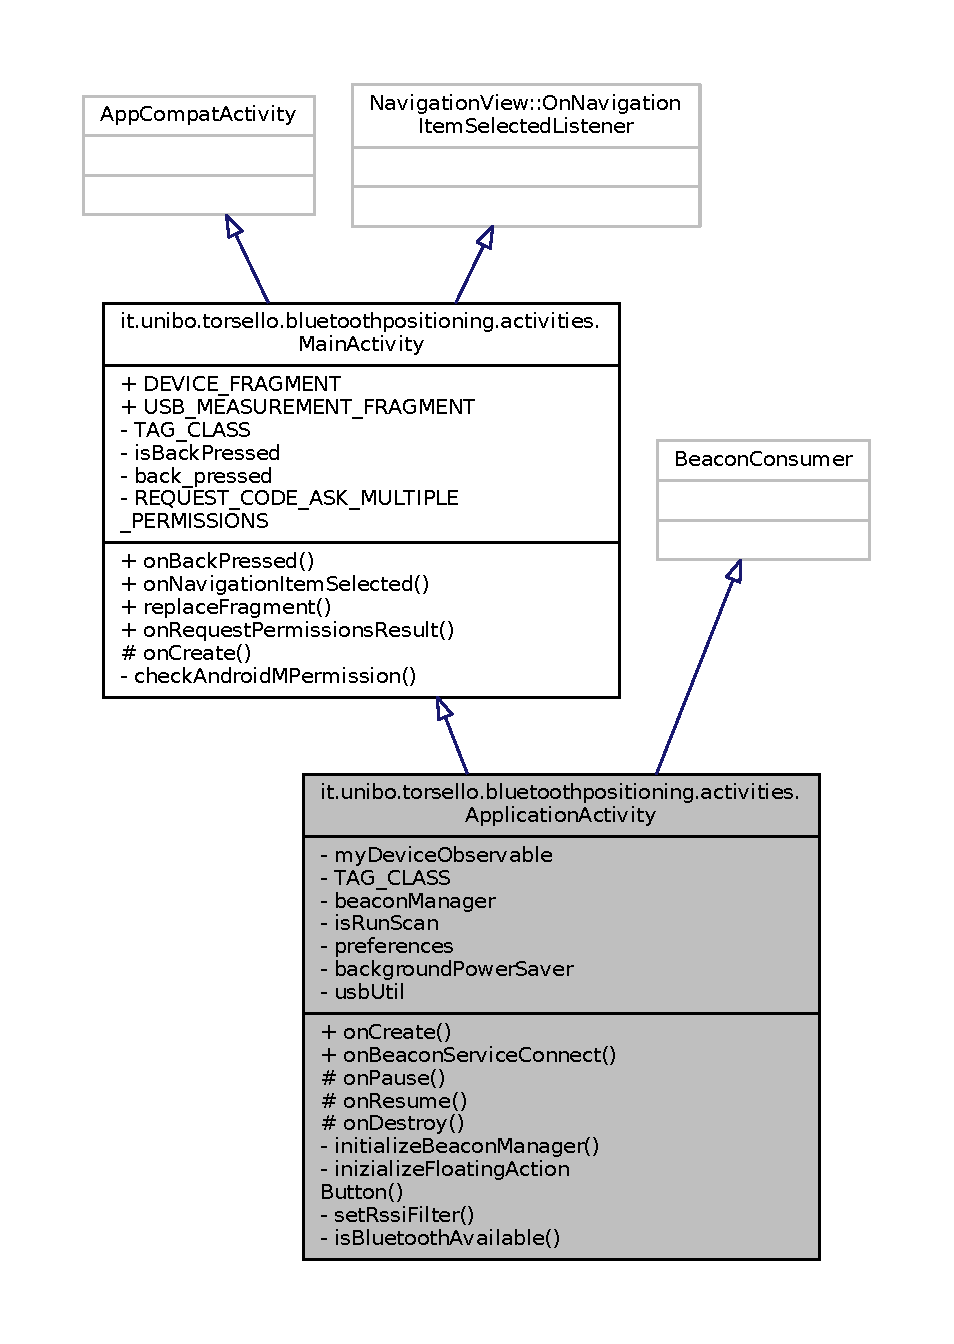
\includegraphics[width=350pt]{classit_1_1unibo_1_1torsello_1_1bluetoothpositioning_1_1activities_1_1ApplicationActivity__inherit__graph}
\end{center}
\end{figure}


Diagramma di collaborazione per it.\+unibo.\+torsello.\+bluetoothpositioning.\+activities.\+Application\+Activity\+:
\nopagebreak
\begin{figure}[H]
\begin{center}
\leavevmode
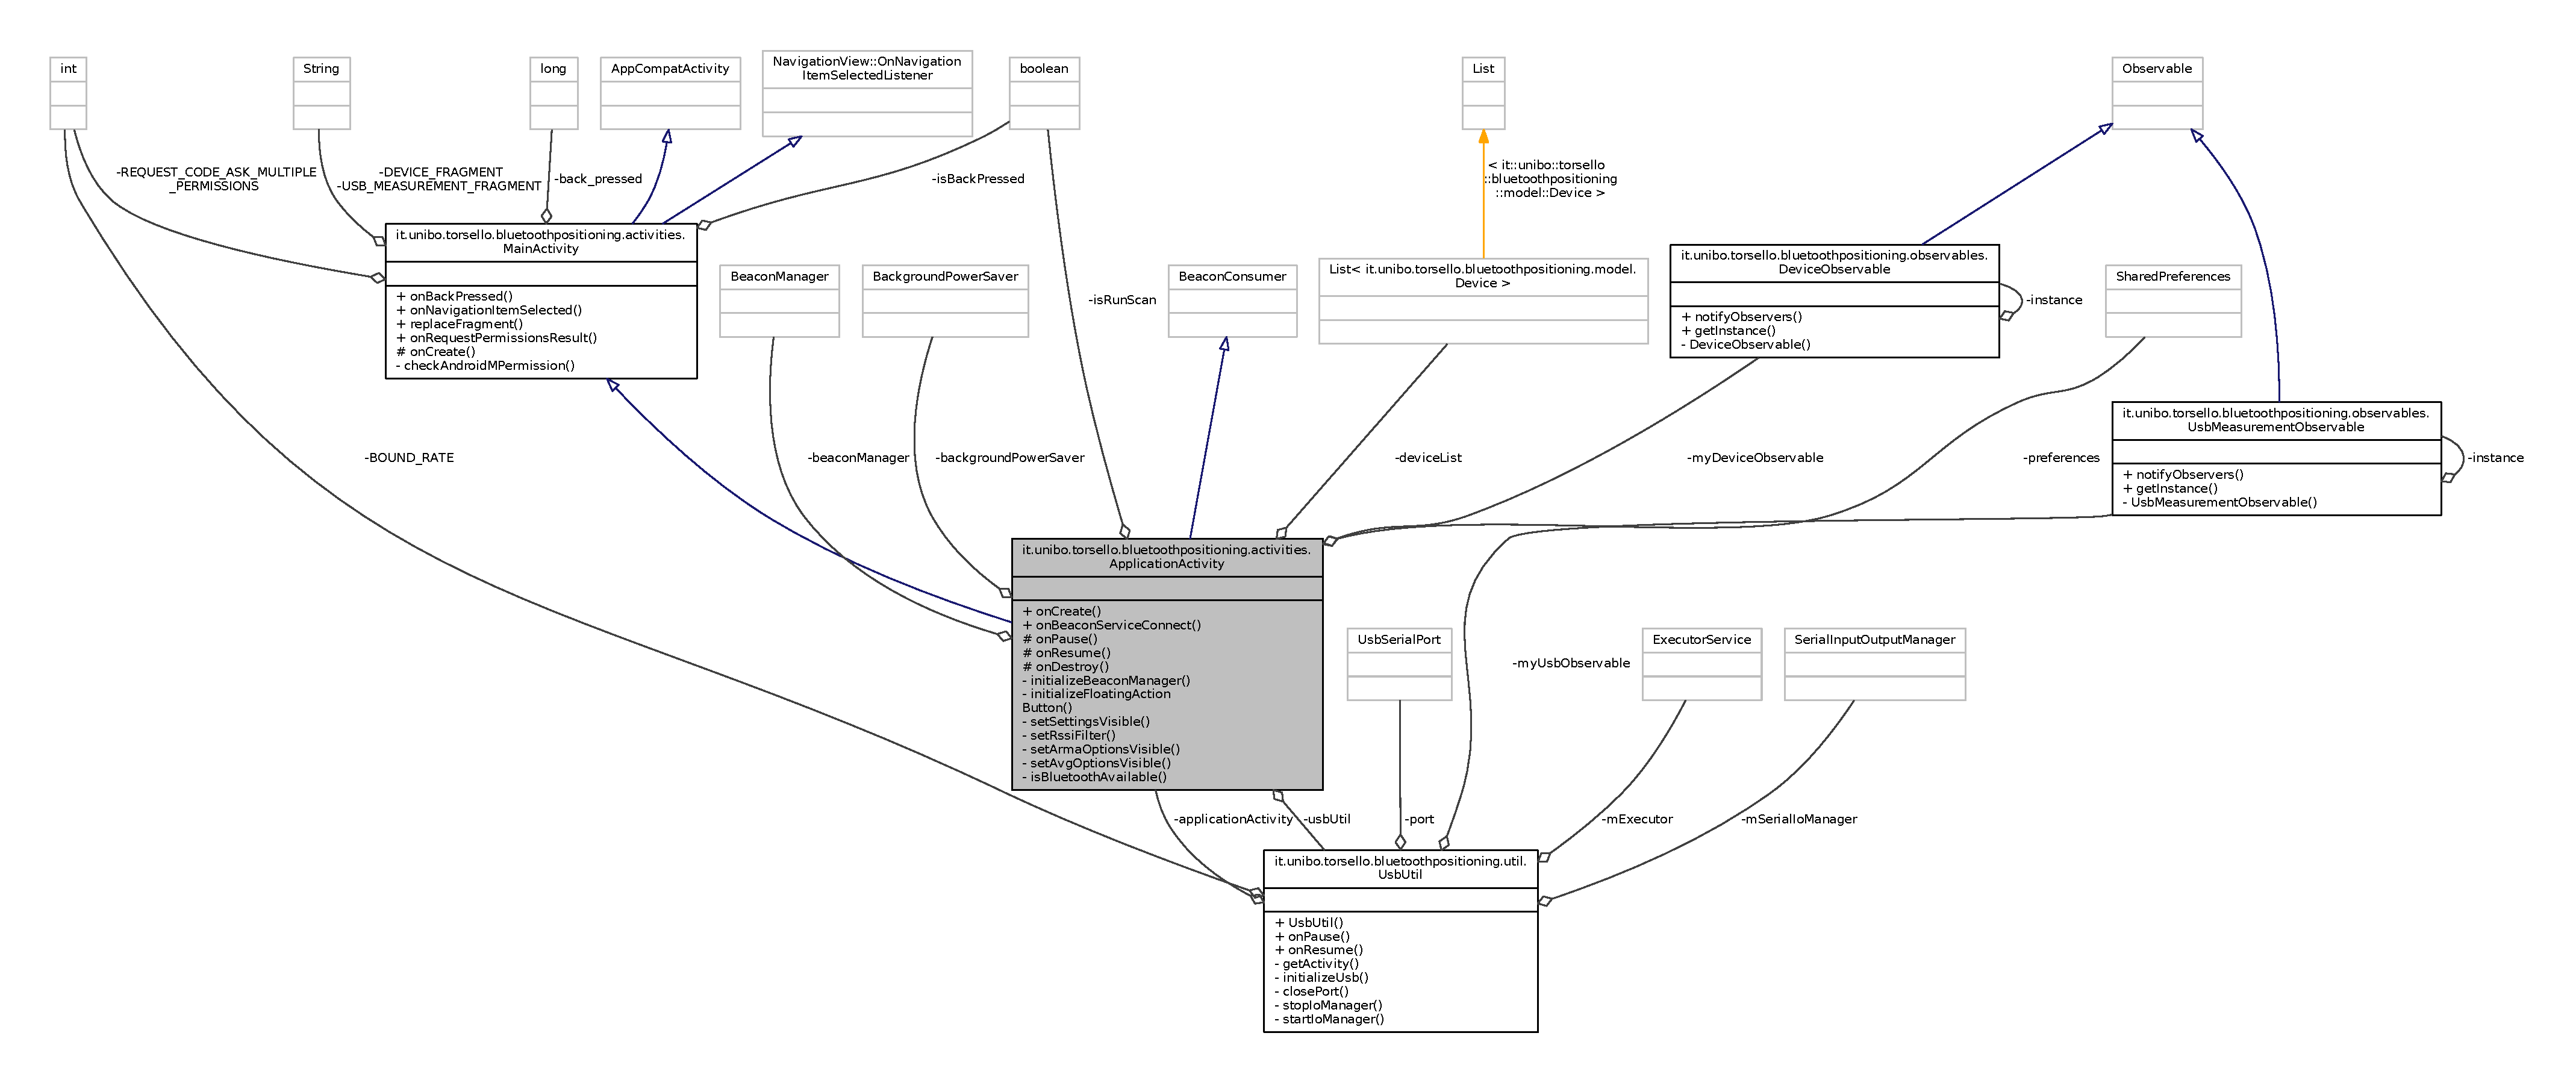
\includegraphics[width=350pt]{classit_1_1unibo_1_1torsello_1_1bluetoothpositioning_1_1activities_1_1ApplicationActivity__coll__graph}
\end{center}
\end{figure}
\subsubsection*{Membri pubblici}
\begin{DoxyCompactItemize}
\item 
void \hyperlink{classit_1_1unibo_1_1torsello_1_1bluetoothpositioning_1_1activities_1_1ApplicationActivity_a395bfa7ec016998b254b9e197ef8d754_a395bfa7ec016998b254b9e197ef8d754}{on\+Create} (Bundle saved\+Instance\+State)
\item 
void \hyperlink{classit_1_1unibo_1_1torsello_1_1bluetoothpositioning_1_1activities_1_1ApplicationActivity_a0cdfc0658ba462b43e9e6b94bab90da1_a0cdfc0658ba462b43e9e6b94bab90da1}{on\+Beacon\+Service\+Connect} ()
\end{DoxyCompactItemize}
\subsubsection*{Membri protetti}
\begin{DoxyCompactItemize}
\item 
void \hyperlink{classit_1_1unibo_1_1torsello_1_1bluetoothpositioning_1_1activities_1_1ApplicationActivity_a06ed1cf654098045b1317b25067af877_a06ed1cf654098045b1317b25067af877}{on\+Pause} ()
\item 
void \hyperlink{classit_1_1unibo_1_1torsello_1_1bluetoothpositioning_1_1activities_1_1ApplicationActivity_ad9e5c029636aac4d7baa2ca8695b3a18_ad9e5c029636aac4d7baa2ca8695b3a18}{on\+Resume} ()
\item 
void \hyperlink{classit_1_1unibo_1_1torsello_1_1bluetoothpositioning_1_1activities_1_1ApplicationActivity_a219ab2598668ab85771f3f8e3c6fec22_a219ab2598668ab85771f3f8e3c6fec22}{on\+Destroy} ()
\end{DoxyCompactItemize}
\subsubsection*{Membri privati}
\begin{DoxyCompactItemize}
\item 
void \hyperlink{classit_1_1unibo_1_1torsello_1_1bluetoothpositioning_1_1activities_1_1ApplicationActivity_a55d4f45ce163b9f613420686f6dfe1cf_a55d4f45ce163b9f613420686f6dfe1cf}{initialize\+Beacon\+Manager} ()
\item 
void \hyperlink{classit_1_1unibo_1_1torsello_1_1bluetoothpositioning_1_1activities_1_1ApplicationActivity_a290aa5909dd27864e0d7d772403ca900_a290aa5909dd27864e0d7d772403ca900}{inizialize\+Floating\+Action\+Button} ()
\item 
void \hyperlink{classit_1_1unibo_1_1torsello_1_1bluetoothpositioning_1_1activities_1_1ApplicationActivity_a8b2514096adfe574c15cc5317a45cd58_a8b2514096adfe574c15cc5317a45cd58}{set\+Rssi\+Filter} ()
\item 
boolean \hyperlink{classit_1_1unibo_1_1torsello_1_1bluetoothpositioning_1_1activities_1_1ApplicationActivity_abffd55741be864ad5b151c8f8c6d70ff_abffd55741be864ad5b151c8f8c6d70ff}{is\+Bluetooth\+Available} ()
\end{DoxyCompactItemize}
\subsubsection*{Attributi privati}
\begin{DoxyCompactItemize}
\item 
Beacon\+Manager \hyperlink{classit_1_1unibo_1_1torsello_1_1bluetoothpositioning_1_1activities_1_1ApplicationActivity_a973c37226a3dbba6016966c3555aff65_a973c37226a3dbba6016966c3555aff65}{beacon\+Manager}
\item 
\hyperlink{classit_1_1unibo_1_1torsello_1_1bluetoothpositioning_1_1observables_1_1DeviceObservable}{Device\+Observable} \hyperlink{classit_1_1unibo_1_1torsello_1_1bluetoothpositioning_1_1activities_1_1ApplicationActivity_aa6481e11e062d3539e6848f0790852b8_aa6481e11e062d3539e6848f0790852b8}{my\+Device\+Observable}
\item 
Shared\+Preferences \hyperlink{classit_1_1unibo_1_1torsello_1_1bluetoothpositioning_1_1activities_1_1ApplicationActivity_a3ee672ef79c268d0618ff3276c2e85f0_a3ee672ef79c268d0618ff3276c2e85f0}{preferences}
\item 
Background\+Power\+Saver \hyperlink{classit_1_1unibo_1_1torsello_1_1bluetoothpositioning_1_1activities_1_1ApplicationActivity_a85885639575161f4d73d4fc788f44ace_a85885639575161f4d73d4fc788f44ace}{background\+Power\+Saver}
\item 
\hyperlink{classit_1_1unibo_1_1torsello_1_1bluetoothpositioning_1_1util_1_1UsbUtil}{Usb\+Util} \hyperlink{classit_1_1unibo_1_1torsello_1_1bluetoothpositioning_1_1activities_1_1ApplicationActivity_abe62157d98c81406ae3d79dbc0fd9093_abe62157d98c81406ae3d79dbc0fd9093}{usb\+Util}
\item 
List$<$ \hyperlink{classit_1_1unibo_1_1torsello_1_1bluetoothpositioning_1_1model_1_1Device}{Device} $>$ \hyperlink{classit_1_1unibo_1_1torsello_1_1bluetoothpositioning_1_1activities_1_1ApplicationActivity_ad146f35cfee210f7191442658a235a2f_ad146f35cfee210f7191442658a235a2f}{device\+List}
\item 
boolean \hyperlink{classit_1_1unibo_1_1torsello_1_1bluetoothpositioning_1_1activities_1_1ApplicationActivity_a16080640c95a73d18c2b7ec21b785af1_a16080640c95a73d18c2b7ec21b785af1}{is\+Run\+Scan} = false
\end{DoxyCompactItemize}
\subsubsection*{Altri membri ereditati}


\subsubsection{Descrizione dettagliata}
Created by Federico Torsello. \href{mailto:federico.torsello@studio.unibo.it}{\tt federico.\+torsello@studio.\+unibo.\+it} 

\subsubsection{Documentazione delle funzioni membro}
\hypertarget{classit_1_1unibo_1_1torsello_1_1bluetoothpositioning_1_1activities_1_1ApplicationActivity_a55d4f45ce163b9f613420686f6dfe1cf_a55d4f45ce163b9f613420686f6dfe1cf}{}\label{classit_1_1unibo_1_1torsello_1_1bluetoothpositioning_1_1activities_1_1ApplicationActivity_a55d4f45ce163b9f613420686f6dfe1cf_a55d4f45ce163b9f613420686f6dfe1cf} 
\index{it\+::unibo\+::torsello\+::bluetoothpositioning\+::activities\+::\+Application\+Activity@{it\+::unibo\+::torsello\+::bluetoothpositioning\+::activities\+::\+Application\+Activity}!initialize\+Beacon\+Manager@{initialize\+Beacon\+Manager}}
\index{initialize\+Beacon\+Manager@{initialize\+Beacon\+Manager}!it\+::unibo\+::torsello\+::bluetoothpositioning\+::activities\+::\+Application\+Activity@{it\+::unibo\+::torsello\+::bluetoothpositioning\+::activities\+::\+Application\+Activity}}
\paragraph{\texorpdfstring{initialize\+Beacon\+Manager()}{initializeBeaconManager()}}
{\footnotesize\ttfamily void it.\+unibo.\+torsello.\+bluetoothpositioning.\+activities.\+Application\+Activity.\+initialize\+Beacon\+Manager (\begin{DoxyParamCaption}{ }\end{DoxyParamCaption})\hspace{0.3cm}{\ttfamily [private]}}


\begin{DoxyCode}
70                                            \{
71         \hyperlink{classit_1_1unibo_1_1torsello_1_1bluetoothpositioning_1_1activities_1_1ApplicationActivity_a973c37226a3dbba6016966c3555aff65_a973c37226a3dbba6016966c3555aff65}{beaconManager} = BeaconManager.getInstanceForApplication(\textcolor{keyword}{this});
72         \hyperlink{classit_1_1unibo_1_1torsello_1_1bluetoothpositioning_1_1activities_1_1ApplicationActivity_a973c37226a3dbba6016966c3555aff65_a973c37226a3dbba6016966c3555aff65}{beaconManager}.bind(\textcolor{keyword}{this});
73 
74         \textcolor{comment}{// Save battery whenever the application is not visible.}
75         \textcolor{comment}{// This reduces bluetooth power usage by about 60%}
76         \hyperlink{classit_1_1unibo_1_1torsello_1_1bluetoothpositioning_1_1activities_1_1ApplicationActivity_a85885639575161f4d73d4fc788f44ace_a85885639575161f4d73d4fc788f44ace}{backgroundPowerSaver} = \textcolor{keyword}{new} BackgroundPowerSaver(\textcolor{keyword}{this});
77 
78 \textcolor{comment}{//        Log.i("AltBeacon filter used:", BeaconManager.getRssiFilterImplClass().getSimpleName());}
79 
80         \textcolor{comment}{// for finding different type of beacon,}
81         \hyperlink{classit_1_1unibo_1_1torsello_1_1bluetoothpositioning_1_1activities_1_1ApplicationActivity_a973c37226a3dbba6016966c3555aff65_a973c37226a3dbba6016966c3555aff65}{beaconManager}.getBeaconParsers().clear();
82 
83         \textcolor{comment}{// Alt beacon}
84         \hyperlink{classit_1_1unibo_1_1torsello_1_1bluetoothpositioning_1_1activities_1_1ApplicationActivity_a973c37226a3dbba6016966c3555aff65_a973c37226a3dbba6016966c3555aff65}{beaconManager}.getBeaconParsers().add(\textcolor{keyword}{new} BeaconParser()
85                 .setBeaconLayout(BeaconParser.ALTBEACON\_LAYOUT));
86         \textcolor{comment}{// Detect the main identifier (UID) frame:}
87         \hyperlink{classit_1_1unibo_1_1torsello_1_1bluetoothpositioning_1_1activities_1_1ApplicationActivity_a973c37226a3dbba6016966c3555aff65_a973c37226a3dbba6016966c3555aff65}{beaconManager}.getBeaconParsers().add(\textcolor{keyword}{new} BeaconParser()
88                 .setBeaconLayout(BeaconParser.EDDYSTONE\_UID\_LAYOUT));
89         \textcolor{comment}{// Detect the telemetry (TLM) frame:}
90         \hyperlink{classit_1_1unibo_1_1torsello_1_1bluetoothpositioning_1_1activities_1_1ApplicationActivity_a973c37226a3dbba6016966c3555aff65_a973c37226a3dbba6016966c3555aff65}{beaconManager}.getBeaconParsers().add(\textcolor{keyword}{new} BeaconParser()
91                 .setBeaconLayout(BeaconParser.EDDYSTONE\_TLM\_LAYOUT));
92         \textcolor{comment}{// Detect the URL frame:}
93         \hyperlink{classit_1_1unibo_1_1torsello_1_1bluetoothpositioning_1_1activities_1_1ApplicationActivity_a973c37226a3dbba6016966c3555aff65_a973c37226a3dbba6016966c3555aff65}{beaconManager}.getBeaconParsers().add(\textcolor{keyword}{new} BeaconParser()
94                 .setBeaconLayout(BeaconParser.EDDYSTONE\_URL\_LAYOUT));
95         \textcolor{comment}{// Standard Apple iBeacon}
96         \hyperlink{classit_1_1unibo_1_1torsello_1_1bluetoothpositioning_1_1activities_1_1ApplicationActivity_a973c37226a3dbba6016966c3555aff65_a973c37226a3dbba6016966c3555aff65}{beaconManager}.getBeaconParsers().add(\textcolor{keyword}{new} BeaconParser()
97                 .setBeaconLayout(DeviceConstants.APPLE\_BEACON\_LAYOUT));
98         \textcolor{comment}{// Estimote Nearable}
99         \hyperlink{classit_1_1unibo_1_1torsello_1_1bluetoothpositioning_1_1activities_1_1ApplicationActivity_a973c37226a3dbba6016966c3555aff65_a973c37226a3dbba6016966c3555aff65}{beaconManager}.getBeaconParsers().add(\textcolor{keyword}{new} BeaconParser()
100                 .setBeaconLayout(DeviceConstants.ESTIMOTE\_NEARABLE\_LAYOUT));
101 
102         \hyperlink{classit_1_1unibo_1_1torsello_1_1bluetoothpositioning_1_1activities_1_1ApplicationActivity_a973c37226a3dbba6016966c3555aff65_a973c37226a3dbba6016966c3555aff65}{beaconManager}.setForegroundScanPeriod(250L);
103         \hyperlink{classit_1_1unibo_1_1torsello_1_1bluetoothpositioning_1_1activities_1_1ApplicationActivity_a973c37226a3dbba6016966c3555aff65_a973c37226a3dbba6016966c3555aff65}{beaconManager}.setForegroundBetweenScanPeriod(0L);
104         \hyperlink{classit_1_1unibo_1_1torsello_1_1bluetoothpositioning_1_1activities_1_1ApplicationActivity_a973c37226a3dbba6016966c3555aff65_a973c37226a3dbba6016966c3555aff65}{beaconManager}.setBackgroundScanPeriod(250L);
105         \hyperlink{classit_1_1unibo_1_1torsello_1_1bluetoothpositioning_1_1activities_1_1ApplicationActivity_a973c37226a3dbba6016966c3555aff65_a973c37226a3dbba6016966c3555aff65}{beaconManager}.setBackgroundBetweenScanPeriod(0L);
106 
107         \hyperlink{classit_1_1unibo_1_1torsello_1_1bluetoothpositioning_1_1activities_1_1ApplicationActivity_a973c37226a3dbba6016966c3555aff65_a973c37226a3dbba6016966c3555aff65}{beaconManager}.setMaxTrackingAge(1000);
108     \}
\end{DoxyCode}
\hypertarget{classit_1_1unibo_1_1torsello_1_1bluetoothpositioning_1_1activities_1_1ApplicationActivity_a290aa5909dd27864e0d7d772403ca900_a290aa5909dd27864e0d7d772403ca900}{}\label{classit_1_1unibo_1_1torsello_1_1bluetoothpositioning_1_1activities_1_1ApplicationActivity_a290aa5909dd27864e0d7d772403ca900_a290aa5909dd27864e0d7d772403ca900} 
\index{it\+::unibo\+::torsello\+::bluetoothpositioning\+::activities\+::\+Application\+Activity@{it\+::unibo\+::torsello\+::bluetoothpositioning\+::activities\+::\+Application\+Activity}!inizialize\+Floating\+Action\+Button@{inizialize\+Floating\+Action\+Button}}
\index{inizialize\+Floating\+Action\+Button@{inizialize\+Floating\+Action\+Button}!it\+::unibo\+::torsello\+::bluetoothpositioning\+::activities\+::\+Application\+Activity@{it\+::unibo\+::torsello\+::bluetoothpositioning\+::activities\+::\+Application\+Activity}}
\paragraph{\texorpdfstring{inizialize\+Floating\+Action\+Button()}{inizializeFloatingActionButton()}}
{\footnotesize\ttfamily void it.\+unibo.\+torsello.\+bluetoothpositioning.\+activities.\+Application\+Activity.\+inizialize\+Floating\+Action\+Button (\begin{DoxyParamCaption}{ }\end{DoxyParamCaption})\hspace{0.3cm}{\ttfamily [private]}}


\begin{DoxyCode}
110                                                   \{
111         \textcolor{keyword}{final} FloatingActionButton fab = (FloatingActionButton) findViewById(R.id.fab);
112         assert fab != null;
113         Snackbar.make(fab, R.string.snackBar\_start\_scanning, Snackbar.LENGTH\_LONG).show();
114         fab.setOnClickListener(\textcolor{keyword}{new} View.OnClickListener() \{
115             @Override
116             \textcolor{keyword}{public} \textcolor{keywordtype}{void} onClick(View view) \{
117 
118                 \textcolor{keywordflow}{if} (\hyperlink{classit_1_1unibo_1_1torsello_1_1bluetoothpositioning_1_1activities_1_1ApplicationActivity_abffd55741be864ad5b151c8f8c6d70ff_abffd55741be864ad5b151c8f8c6d70ff}{isBluetoothAvailable}()) \{
119 
120                     \hyperlink{classit_1_1unibo_1_1torsello_1_1bluetoothpositioning_1_1activities_1_1ApplicationActivity_a16080640c95a73d18c2b7ec21b785af1_a16080640c95a73d18c2b7ec21b785af1}{isRunScan} = !\hyperlink{classit_1_1unibo_1_1torsello_1_1bluetoothpositioning_1_1activities_1_1ApplicationActivity_a16080640c95a73d18c2b7ec21b785af1_a16080640c95a73d18c2b7ec21b785af1}{isRunScan};
121                     Region region = \textcolor{keyword}{new} Region(\textcolor{stringliteral}{"RegionId"}, null, null, null);
122 
123                     \textcolor{keywordflow}{if} (\hyperlink{classit_1_1unibo_1_1torsello_1_1bluetoothpositioning_1_1activities_1_1ApplicationActivity_a16080640c95a73d18c2b7ec21b785af1_a16080640c95a73d18c2b7ec21b785af1}{isRunScan}) \{
124                         fab.setImageResource(R.drawable.ic\_bluetooth\_searching\_white\_24dp);
125                         \textcolor{keywordflow}{try} \{
126                             \hyperlink{classit_1_1unibo_1_1torsello_1_1bluetoothpositioning_1_1activities_1_1ApplicationActivity_a973c37226a3dbba6016966c3555aff65_a973c37226a3dbba6016966c3555aff65}{beaconManager}.startRangingBeaconsInRegion(region);
127                         \} \textcolor{keywordflow}{catch} (RemoteException e) \{
128                             e.printStackTrace();
129                         \}
130                         Snackbar.make(view, R.string.snackBar\_scanning\_enabled,
131                                 Snackbar.LENGTH\_SHORT).show();
132                     \} \textcolor{keywordflow}{else} \{
133                         fab.setImageResource(R.drawable.ic\_bluetooth\_white\_24dp);
134                         \textcolor{keywordflow}{try} \{
135                             \hyperlink{classit_1_1unibo_1_1torsello_1_1bluetoothpositioning_1_1activities_1_1ApplicationActivity_a973c37226a3dbba6016966c3555aff65_a973c37226a3dbba6016966c3555aff65}{beaconManager}.stopRangingBeaconsInRegion(region);
136                         \} \textcolor{keywordflow}{catch} (RemoteException e) \{
137                             e.printStackTrace();
138                         \}
139                         Snackbar.make(view, R.string.snackBar\_scanning\_disabled,
140                                 Snackbar.LENGTH\_INDEFINITE).show();
141                     \}
142                 \}
143             \}
144         \});
145     \}
\end{DoxyCode}
\hypertarget{classit_1_1unibo_1_1torsello_1_1bluetoothpositioning_1_1activities_1_1ApplicationActivity_abffd55741be864ad5b151c8f8c6d70ff_abffd55741be864ad5b151c8f8c6d70ff}{}\label{classit_1_1unibo_1_1torsello_1_1bluetoothpositioning_1_1activities_1_1ApplicationActivity_abffd55741be864ad5b151c8f8c6d70ff_abffd55741be864ad5b151c8f8c6d70ff} 
\index{it\+::unibo\+::torsello\+::bluetoothpositioning\+::activities\+::\+Application\+Activity@{it\+::unibo\+::torsello\+::bluetoothpositioning\+::activities\+::\+Application\+Activity}!is\+Bluetooth\+Available@{is\+Bluetooth\+Available}}
\index{is\+Bluetooth\+Available@{is\+Bluetooth\+Available}!it\+::unibo\+::torsello\+::bluetoothpositioning\+::activities\+::\+Application\+Activity@{it\+::unibo\+::torsello\+::bluetoothpositioning\+::activities\+::\+Application\+Activity}}
\paragraph{\texorpdfstring{is\+Bluetooth\+Available()}{isBluetoothAvailable()}}
{\footnotesize\ttfamily boolean it.\+unibo.\+torsello.\+bluetoothpositioning.\+activities.\+Application\+Activity.\+is\+Bluetooth\+Available (\begin{DoxyParamCaption}{ }\end{DoxyParamCaption})\hspace{0.3cm}{\ttfamily [private]}}


\begin{DoxyCode}
250                                            \{
251 
252         \textcolor{keywordflow}{try} \{
253             \textcolor{keywordflow}{if} (!\hyperlink{classit_1_1unibo_1_1torsello_1_1bluetoothpositioning_1_1activities_1_1ApplicationActivity_a973c37226a3dbba6016966c3555aff65_a973c37226a3dbba6016966c3555aff65}{beaconManager}.checkAvailability()) \{
254 
255                 \textcolor{keyword}{final} FloatingActionButton fab = (FloatingActionButton) findViewById(R.id.fab);
256                 assert fab != null;
257 
258                 \textcolor{keyword}{new} AlertDialog.Builder(\textcolor{keyword}{this})
259                         .setTitle(R.string.dialog\_bluetooth\_title)
260                         .setMessage(R.string.dialog\_bluetooth\_text)
261                         .setPositiveButton(android.R.string.ok, null)
262                         .setOnDismissListener(\textcolor{keyword}{new} DialogInterface.OnDismissListener() \{
263                             @Override
264                             \textcolor{keyword}{public} \textcolor{keywordtype}{void} onDismiss(DialogInterface dialog) \{
265                                 fab.setImageResource(R.drawable.ic\_bluetooth\_white\_24dp);
266                                 BluetoothAdapter.getDefaultAdapter().enable();
267                             \}
268                         \}).show();
269                 fab.setImageResource(R.drawable.ic\_bluetooth\_disabled\_black\_24dp);
270                 \textcolor{keywordflow}{return} \textcolor{keyword}{false};
271             \}
272         \} \textcolor{keywordflow}{catch} (RuntimeException e) \{
273             e.getStackTrace();
274         \}
275         \textcolor{keywordflow}{return} \textcolor{keyword}{true};
276     \}
\end{DoxyCode}
\hypertarget{classit_1_1unibo_1_1torsello_1_1bluetoothpositioning_1_1activities_1_1ApplicationActivity_a0cdfc0658ba462b43e9e6b94bab90da1_a0cdfc0658ba462b43e9e6b94bab90da1}{}\label{classit_1_1unibo_1_1torsello_1_1bluetoothpositioning_1_1activities_1_1ApplicationActivity_a0cdfc0658ba462b43e9e6b94bab90da1_a0cdfc0658ba462b43e9e6b94bab90da1} 
\index{it\+::unibo\+::torsello\+::bluetoothpositioning\+::activities\+::\+Application\+Activity@{it\+::unibo\+::torsello\+::bluetoothpositioning\+::activities\+::\+Application\+Activity}!on\+Beacon\+Service\+Connect@{on\+Beacon\+Service\+Connect}}
\index{on\+Beacon\+Service\+Connect@{on\+Beacon\+Service\+Connect}!it\+::unibo\+::torsello\+::bluetoothpositioning\+::activities\+::\+Application\+Activity@{it\+::unibo\+::torsello\+::bluetoothpositioning\+::activities\+::\+Application\+Activity}}
\paragraph{\texorpdfstring{on\+Beacon\+Service\+Connect()}{onBeaconServiceConnect()}}
{\footnotesize\ttfamily void it.\+unibo.\+torsello.\+bluetoothpositioning.\+activities.\+Application\+Activity.\+on\+Beacon\+Service\+Connect (\begin{DoxyParamCaption}{ }\end{DoxyParamCaption})}


\begin{DoxyCode}
148                                          \{
149 
150         \textcolor{keywordflow}{try} \{
151             \hyperlink{classit_1_1unibo_1_1torsello_1_1bluetoothpositioning_1_1activities_1_1ApplicationActivity_a973c37226a3dbba6016966c3555aff65_a973c37226a3dbba6016966c3555aff65}{beaconManager}.updateScanPeriods();
152         \} \textcolor{keywordflow}{catch} (RemoteException e) \{
153             e.printStackTrace();
154         \}
155 
156         \hyperlink{classit_1_1unibo_1_1torsello_1_1bluetoothpositioning_1_1activities_1_1ApplicationActivity_a973c37226a3dbba6016966c3555aff65_a973c37226a3dbba6016966c3555aff65}{beaconManager}.addRangeNotifier(\textcolor{keyword}{new} RangeNotifier() \{
157             @Override
158             \textcolor{keyword}{public} \textcolor{keywordtype}{void} didRangeBeaconsInRegion(\textcolor{keyword}{final} Collection<Beacon> beacons, Region region) \{
159 
160                 \hyperlink{classit_1_1unibo_1_1torsello_1_1bluetoothpositioning_1_1activities_1_1ApplicationActivity_a8b2514096adfe574c15cc5317a45cd58_a8b2514096adfe574c15cc5317a45cd58}{setRssiFilter}();
161 
162                 \textcolor{keywordflow}{for} (Beacon b : beacons) \{
163 
164                     \textcolor{comment}{// take from the list the device}
165                     Device device = DeviceConstants.DEVICE\_MAP.get(b.getBluetoothAddress());
166 
167                     \textcolor{keywordflow}{if} (device != null) \{ \textcolor{comment}{// useful only if DEVICE\_MAP is empty}
168                         \textcolor{keywordtype}{double} processNoise = \hyperlink{classit_1_1unibo_1_1torsello_1_1bluetoothpositioning_1_1activities_1_1ApplicationActivity_a3ee672ef79c268d0618ff3276c2e85f0_a3ee672ef79c268d0618ff3276c2e85f0}{preferences}.getFloat(SettingConstants.
      KALMAN\_NOISE\_VALUE, 0);
169                         device.setBeacon(b);
170                         device.updateDistance(processNoise);
171 
172                         \textcolor{keywordflow}{if} (!\hyperlink{classit_1_1unibo_1_1torsello_1_1bluetoothpositioning_1_1activities_1_1ApplicationActivity_ad146f35cfee210f7191442658a235a2f_ad146f35cfee210f7191442658a235a2f}{deviceList}.contains(device)) \{
173                             \hyperlink{classit_1_1unibo_1_1torsello_1_1bluetoothpositioning_1_1activities_1_1ApplicationActivity_ad146f35cfee210f7191442658a235a2f_ad146f35cfee210f7191442658a235a2f}{deviceList}.add(device);
174                         \}
175                     \}
176                 \}
177 
178                 \textcolor{keyword}{new} Thread(\textcolor{keyword}{new} Runnable() \{
179                     @Override
180                     \textcolor{keyword}{public} \textcolor{keywordtype}{void} run() \{
181                         runOnUiThread(\textcolor{keyword}{new} Runnable() \{
182 
183                             @Override
184                             \textcolor{keyword}{public} \textcolor{keywordtype}{void} run() \{
185                                 \hyperlink{classit_1_1unibo_1_1torsello_1_1bluetoothpositioning_1_1activities_1_1ApplicationActivity_aa6481e11e062d3539e6848f0790852b8_aa6481e11e062d3539e6848f0790852b8}{myDeviceObservable}.
      \hyperlink{classit_1_1unibo_1_1torsello_1_1bluetoothpositioning_1_1observables_1_1DeviceObservable_aaf183e537e44cbd114c8eb76432da191_aaf183e537e44cbd114c8eb76432da191}{notifyObservers}(\hyperlink{classit_1_1unibo_1_1torsello_1_1bluetoothpositioning_1_1activities_1_1ApplicationActivity_ad146f35cfee210f7191442658a235a2f_ad146f35cfee210f7191442658a235a2f}{deviceList});
186                             \}
187                         \});
188                     \}
189                 \}).start();
190             \}
191         \});
192     \}
\end{DoxyCode}
\hypertarget{classit_1_1unibo_1_1torsello_1_1bluetoothpositioning_1_1activities_1_1ApplicationActivity_a395bfa7ec016998b254b9e197ef8d754_a395bfa7ec016998b254b9e197ef8d754}{}\label{classit_1_1unibo_1_1torsello_1_1bluetoothpositioning_1_1activities_1_1ApplicationActivity_a395bfa7ec016998b254b9e197ef8d754_a395bfa7ec016998b254b9e197ef8d754} 
\index{it\+::unibo\+::torsello\+::bluetoothpositioning\+::activities\+::\+Application\+Activity@{it\+::unibo\+::torsello\+::bluetoothpositioning\+::activities\+::\+Application\+Activity}!on\+Create@{on\+Create}}
\index{on\+Create@{on\+Create}!it\+::unibo\+::torsello\+::bluetoothpositioning\+::activities\+::\+Application\+Activity@{it\+::unibo\+::torsello\+::bluetoothpositioning\+::activities\+::\+Application\+Activity}}
\paragraph{\texorpdfstring{on\+Create()}{onCreate()}}
{\footnotesize\ttfamily void it.\+unibo.\+torsello.\+bluetoothpositioning.\+activities.\+Application\+Activity.\+on\+Create (\begin{DoxyParamCaption}\item[{Bundle}]{saved\+Instance\+State }\end{DoxyParamCaption})}


\begin{DoxyCode}
54                                                     \{
55         super.onCreate(savedInstanceState);
56 
57         \hyperlink{classit_1_1unibo_1_1torsello_1_1bluetoothpositioning_1_1activities_1_1ApplicationActivity_ad146f35cfee210f7191442658a235a2f_ad146f35cfee210f7191442658a235a2f}{deviceList} = \textcolor{keyword}{new} ArrayList<>();
58 
59         \hyperlink{classit_1_1unibo_1_1torsello_1_1bluetoothpositioning_1_1activities_1_1ApplicationActivity_aa6481e11e062d3539e6848f0790852b8_aa6481e11e062d3539e6848f0790852b8}{myDeviceObservable} = DeviceObservable.\hyperlink{classit_1_1unibo_1_1torsello_1_1bluetoothpositioning_1_1observables_1_1DeviceObservable_ab16792c5848440646624b2a41553954a_ab16792c5848440646624b2a41553954a}{getInstance}();
60 
61         \hyperlink{classit_1_1unibo_1_1torsello_1_1bluetoothpositioning_1_1activities_1_1ApplicationActivity_a3ee672ef79c268d0618ff3276c2e85f0_a3ee672ef79c268d0618ff3276c2e85f0}{preferences} = getSharedPreferences(SettingConstants.SETTINGS\_PREFERENCES, 0);
62 
63         \hyperlink{classit_1_1unibo_1_1torsello_1_1bluetoothpositioning_1_1activities_1_1ApplicationActivity_abe62157d98c81406ae3d79dbc0fd9093_abe62157d98c81406ae3d79dbc0fd9093}{usbUtil} = \textcolor{keyword}{new} UsbUtil(\textcolor{keyword}{this});
64 
65         \hyperlink{classit_1_1unibo_1_1torsello_1_1bluetoothpositioning_1_1activities_1_1ApplicationActivity_a55d4f45ce163b9f613420686f6dfe1cf_a55d4f45ce163b9f613420686f6dfe1cf}{initializeBeaconManager}();
66 
67         \hyperlink{classit_1_1unibo_1_1torsello_1_1bluetoothpositioning_1_1activities_1_1ApplicationActivity_a290aa5909dd27864e0d7d772403ca900_a290aa5909dd27864e0d7d772403ca900}{inizializeFloatingActionButton}();
68     \}
\end{DoxyCode}
\hypertarget{classit_1_1unibo_1_1torsello_1_1bluetoothpositioning_1_1activities_1_1ApplicationActivity_a219ab2598668ab85771f3f8e3c6fec22_a219ab2598668ab85771f3f8e3c6fec22}{}\label{classit_1_1unibo_1_1torsello_1_1bluetoothpositioning_1_1activities_1_1ApplicationActivity_a219ab2598668ab85771f3f8e3c6fec22_a219ab2598668ab85771f3f8e3c6fec22} 
\index{it\+::unibo\+::torsello\+::bluetoothpositioning\+::activities\+::\+Application\+Activity@{it\+::unibo\+::torsello\+::bluetoothpositioning\+::activities\+::\+Application\+Activity}!on\+Destroy@{on\+Destroy}}
\index{on\+Destroy@{on\+Destroy}!it\+::unibo\+::torsello\+::bluetoothpositioning\+::activities\+::\+Application\+Activity@{it\+::unibo\+::torsello\+::bluetoothpositioning\+::activities\+::\+Application\+Activity}}
\paragraph{\texorpdfstring{on\+Destroy()}{onDestroy()}}
{\footnotesize\ttfamily void it.\+unibo.\+torsello.\+bluetoothpositioning.\+activities.\+Application\+Activity.\+on\+Destroy (\begin{DoxyParamCaption}{ }\end{DoxyParamCaption})\hspace{0.3cm}{\ttfamily [protected]}}


\begin{DoxyCode}
241                                \{
242         \textcolor{keywordflow}{if} (\hyperlink{classit_1_1unibo_1_1torsello_1_1bluetoothpositioning_1_1activities_1_1ApplicationActivity_a973c37226a3dbba6016966c3555aff65_a973c37226a3dbba6016966c3555aff65}{beaconManager}.isBound(\textcolor{keyword}{this})) \{
243             \hyperlink{classit_1_1unibo_1_1torsello_1_1bluetoothpositioning_1_1activities_1_1ApplicationActivity_a973c37226a3dbba6016966c3555aff65_a973c37226a3dbba6016966c3555aff65}{beaconManager}.unbind(\textcolor{keyword}{this});
244             \hyperlink{classit_1_1unibo_1_1torsello_1_1bluetoothpositioning_1_1activities_1_1ApplicationActivity_a85885639575161f4d73d4fc788f44ace_a85885639575161f4d73d4fc788f44ace}{backgroundPowerSaver}.onActivityDestroyed(\textcolor{keyword}{this});
245         \}
246 
247         super.onDestroy();
248     \}
\end{DoxyCode}
\hypertarget{classit_1_1unibo_1_1torsello_1_1bluetoothpositioning_1_1activities_1_1ApplicationActivity_a06ed1cf654098045b1317b25067af877_a06ed1cf654098045b1317b25067af877}{}\label{classit_1_1unibo_1_1torsello_1_1bluetoothpositioning_1_1activities_1_1ApplicationActivity_a06ed1cf654098045b1317b25067af877_a06ed1cf654098045b1317b25067af877} 
\index{it\+::unibo\+::torsello\+::bluetoothpositioning\+::activities\+::\+Application\+Activity@{it\+::unibo\+::torsello\+::bluetoothpositioning\+::activities\+::\+Application\+Activity}!on\+Pause@{on\+Pause}}
\index{on\+Pause@{on\+Pause}!it\+::unibo\+::torsello\+::bluetoothpositioning\+::activities\+::\+Application\+Activity@{it\+::unibo\+::torsello\+::bluetoothpositioning\+::activities\+::\+Application\+Activity}}
\paragraph{\texorpdfstring{on\+Pause()}{onPause()}}
{\footnotesize\ttfamily void it.\+unibo.\+torsello.\+bluetoothpositioning.\+activities.\+Application\+Activity.\+on\+Pause (\begin{DoxyParamCaption}{ }\end{DoxyParamCaption})\hspace{0.3cm}{\ttfamily [protected]}}


\begin{DoxyCode}
214                              \{
215         \textcolor{keywordflow}{if} (\hyperlink{classit_1_1unibo_1_1torsello_1_1bluetoothpositioning_1_1activities_1_1ApplicationActivity_a973c37226a3dbba6016966c3555aff65_a973c37226a3dbba6016966c3555aff65}{beaconManager}.isBound(\textcolor{keyword}{this})) \{
216             \hyperlink{classit_1_1unibo_1_1torsello_1_1bluetoothpositioning_1_1activities_1_1ApplicationActivity_a973c37226a3dbba6016966c3555aff65_a973c37226a3dbba6016966c3555aff65}{beaconManager}.setBackgroundMode(\textcolor{keyword}{true});
217             \hyperlink{classit_1_1unibo_1_1torsello_1_1bluetoothpositioning_1_1activities_1_1ApplicationActivity_a85885639575161f4d73d4fc788f44ace_a85885639575161f4d73d4fc788f44ace}{backgroundPowerSaver}.onActivityPaused(\textcolor{keyword}{this});
218         \}
219 
220         \hyperlink{classit_1_1unibo_1_1torsello_1_1bluetoothpositioning_1_1activities_1_1ApplicationActivity_abe62157d98c81406ae3d79dbc0fd9093_abe62157d98c81406ae3d79dbc0fd9093}{usbUtil}.\hyperlink{classit_1_1unibo_1_1torsello_1_1bluetoothpositioning_1_1util_1_1UsbUtil_ab4f2c73fa6b776c9d4967ff89da0d8ca_ab4f2c73fa6b776c9d4967ff89da0d8ca}{onPause}();
221 
222         super.onPause();
223     \}
\end{DoxyCode}
\hypertarget{classit_1_1unibo_1_1torsello_1_1bluetoothpositioning_1_1activities_1_1ApplicationActivity_ad9e5c029636aac4d7baa2ca8695b3a18_ad9e5c029636aac4d7baa2ca8695b3a18}{}\label{classit_1_1unibo_1_1torsello_1_1bluetoothpositioning_1_1activities_1_1ApplicationActivity_ad9e5c029636aac4d7baa2ca8695b3a18_ad9e5c029636aac4d7baa2ca8695b3a18} 
\index{it\+::unibo\+::torsello\+::bluetoothpositioning\+::activities\+::\+Application\+Activity@{it\+::unibo\+::torsello\+::bluetoothpositioning\+::activities\+::\+Application\+Activity}!on\+Resume@{on\+Resume}}
\index{on\+Resume@{on\+Resume}!it\+::unibo\+::torsello\+::bluetoothpositioning\+::activities\+::\+Application\+Activity@{it\+::unibo\+::torsello\+::bluetoothpositioning\+::activities\+::\+Application\+Activity}}
\paragraph{\texorpdfstring{on\+Resume()}{onResume()}}
{\footnotesize\ttfamily void it.\+unibo.\+torsello.\+bluetoothpositioning.\+activities.\+Application\+Activity.\+on\+Resume (\begin{DoxyParamCaption}{ }\end{DoxyParamCaption})\hspace{0.3cm}{\ttfamily [protected]}}


\begin{DoxyCode}
226                               \{
227         super.onResume();
228 
229         \textcolor{keywordflow}{if} (\hyperlink{classit_1_1unibo_1_1torsello_1_1bluetoothpositioning_1_1activities_1_1ApplicationActivity_a973c37226a3dbba6016966c3555aff65_a973c37226a3dbba6016966c3555aff65}{beaconManager}.isBound(\textcolor{keyword}{this})) \{
230             \hyperlink{classit_1_1unibo_1_1torsello_1_1bluetoothpositioning_1_1activities_1_1ApplicationActivity_a973c37226a3dbba6016966c3555aff65_a973c37226a3dbba6016966c3555aff65}{beaconManager}.setBackgroundMode(\textcolor{keyword}{false});
231             \hyperlink{classit_1_1unibo_1_1torsello_1_1bluetoothpositioning_1_1activities_1_1ApplicationActivity_a85885639575161f4d73d4fc788f44ace_a85885639575161f4d73d4fc788f44ace}{backgroundPowerSaver}.onActivityResumed(\textcolor{keyword}{this});
232         \}
233 
234         \hyperlink{classit_1_1unibo_1_1torsello_1_1bluetoothpositioning_1_1activities_1_1ApplicationActivity_abffd55741be864ad5b151c8f8c6d70ff_abffd55741be864ad5b151c8f8c6d70ff}{isBluetoothAvailable}();
235 
236         \hyperlink{classit_1_1unibo_1_1torsello_1_1bluetoothpositioning_1_1activities_1_1ApplicationActivity_abe62157d98c81406ae3d79dbc0fd9093_abe62157d98c81406ae3d79dbc0fd9093}{usbUtil}.\hyperlink{classit_1_1unibo_1_1torsello_1_1bluetoothpositioning_1_1util_1_1UsbUtil_ae814610c8dc793fea3a9a314fb26e3cb_ae814610c8dc793fea3a9a314fb26e3cb}{onResume}();
237 
238     \}
\end{DoxyCode}
\hypertarget{classit_1_1unibo_1_1torsello_1_1bluetoothpositioning_1_1activities_1_1ApplicationActivity_a8b2514096adfe574c15cc5317a45cd58_a8b2514096adfe574c15cc5317a45cd58}{}\label{classit_1_1unibo_1_1torsello_1_1bluetoothpositioning_1_1activities_1_1ApplicationActivity_a8b2514096adfe574c15cc5317a45cd58_a8b2514096adfe574c15cc5317a45cd58} 
\index{it\+::unibo\+::torsello\+::bluetoothpositioning\+::activities\+::\+Application\+Activity@{it\+::unibo\+::torsello\+::bluetoothpositioning\+::activities\+::\+Application\+Activity}!set\+Rssi\+Filter@{set\+Rssi\+Filter}}
\index{set\+Rssi\+Filter@{set\+Rssi\+Filter}!it\+::unibo\+::torsello\+::bluetoothpositioning\+::activities\+::\+Application\+Activity@{it\+::unibo\+::torsello\+::bluetoothpositioning\+::activities\+::\+Application\+Activity}}
\paragraph{\texorpdfstring{set\+Rssi\+Filter()}{setRssiFilter()}}
{\footnotesize\ttfamily void it.\+unibo.\+torsello.\+bluetoothpositioning.\+activities.\+Application\+Activity.\+set\+Rssi\+Filter (\begin{DoxyParamCaption}{ }\end{DoxyParamCaption})\hspace{0.3cm}{\ttfamily [private]}}


\begin{DoxyCode}
194                                  \{
195 
196         \textcolor{keywordtype}{int} sorting = \hyperlink{classit_1_1unibo_1_1torsello_1_1bluetoothpositioning_1_1activities_1_1ApplicationActivity_a3ee672ef79c268d0618ff3276c2e85f0_a3ee672ef79c268d0618ff3276c2e85f0}{preferences}.getInt(SettingConstants.FILTER\_RSSI, 0);
197         \textcolor{keywordflow}{switch} (sorting) \{
198             \textcolor{keywordflow}{case} 0:
199             \textcolor{keywordflow}{case} R.id.radioButton\_no\_rssi\_filtering:
200                 MyArmaRssiFilter.enableArmaFilter(\textcolor{keyword}{false});
201                 BeaconManager.setRssiFilterImplClass(MyArmaRssiFilter.class);
202                 \textcolor{keywordflow}{break};
203             \textcolor{keywordflow}{case} R.id.radioButton\_arma\_rssi\_filter:
204                 MyArmaRssiFilter.enableArmaFilter(\textcolor{keyword}{true});
205                 BeaconManager.setRssiFilterImplClass(MyArmaRssiFilter.class);
206                 \textcolor{keywordflow}{break};
207             \textcolor{keywordflow}{case} R.id.radioButton\_average\_rssi\_filter:
208                 BeaconManager.setRssiFilterImplClass(RunningAverageRssiFilter.class);
209                 \textcolor{keywordflow}{break};
210         \}
211     \}
\end{DoxyCode}


\subsubsection{Documentazione dei membri dato}
\hypertarget{classit_1_1unibo_1_1torsello_1_1bluetoothpositioning_1_1activities_1_1ApplicationActivity_a85885639575161f4d73d4fc788f44ace_a85885639575161f4d73d4fc788f44ace}{}\label{classit_1_1unibo_1_1torsello_1_1bluetoothpositioning_1_1activities_1_1ApplicationActivity_a85885639575161f4d73d4fc788f44ace_a85885639575161f4d73d4fc788f44ace} 
\index{it\+::unibo\+::torsello\+::bluetoothpositioning\+::activities\+::\+Application\+Activity@{it\+::unibo\+::torsello\+::bluetoothpositioning\+::activities\+::\+Application\+Activity}!background\+Power\+Saver@{background\+Power\+Saver}}
\index{background\+Power\+Saver@{background\+Power\+Saver}!it\+::unibo\+::torsello\+::bluetoothpositioning\+::activities\+::\+Application\+Activity@{it\+::unibo\+::torsello\+::bluetoothpositioning\+::activities\+::\+Application\+Activity}}
\paragraph{\texorpdfstring{background\+Power\+Saver}{backgroundPowerSaver}}
{\footnotesize\ttfamily Background\+Power\+Saver it.\+unibo.\+torsello.\+bluetoothpositioning.\+activities.\+Application\+Activity.\+background\+Power\+Saver\hspace{0.3cm}{\ttfamily [private]}}

\hypertarget{classit_1_1unibo_1_1torsello_1_1bluetoothpositioning_1_1activities_1_1ApplicationActivity_a973c37226a3dbba6016966c3555aff65_a973c37226a3dbba6016966c3555aff65}{}\label{classit_1_1unibo_1_1torsello_1_1bluetoothpositioning_1_1activities_1_1ApplicationActivity_a973c37226a3dbba6016966c3555aff65_a973c37226a3dbba6016966c3555aff65} 
\index{it\+::unibo\+::torsello\+::bluetoothpositioning\+::activities\+::\+Application\+Activity@{it\+::unibo\+::torsello\+::bluetoothpositioning\+::activities\+::\+Application\+Activity}!beacon\+Manager@{beacon\+Manager}}
\index{beacon\+Manager@{beacon\+Manager}!it\+::unibo\+::torsello\+::bluetoothpositioning\+::activities\+::\+Application\+Activity@{it\+::unibo\+::torsello\+::bluetoothpositioning\+::activities\+::\+Application\+Activity}}
\paragraph{\texorpdfstring{beacon\+Manager}{beaconManager}}
{\footnotesize\ttfamily Beacon\+Manager it.\+unibo.\+torsello.\+bluetoothpositioning.\+activities.\+Application\+Activity.\+beacon\+Manager\hspace{0.3cm}{\ttfamily [private]}}

\hypertarget{classit_1_1unibo_1_1torsello_1_1bluetoothpositioning_1_1activities_1_1ApplicationActivity_ad146f35cfee210f7191442658a235a2f_ad146f35cfee210f7191442658a235a2f}{}\label{classit_1_1unibo_1_1torsello_1_1bluetoothpositioning_1_1activities_1_1ApplicationActivity_ad146f35cfee210f7191442658a235a2f_ad146f35cfee210f7191442658a235a2f} 
\index{it\+::unibo\+::torsello\+::bluetoothpositioning\+::activities\+::\+Application\+Activity@{it\+::unibo\+::torsello\+::bluetoothpositioning\+::activities\+::\+Application\+Activity}!device\+List@{device\+List}}
\index{device\+List@{device\+List}!it\+::unibo\+::torsello\+::bluetoothpositioning\+::activities\+::\+Application\+Activity@{it\+::unibo\+::torsello\+::bluetoothpositioning\+::activities\+::\+Application\+Activity}}
\paragraph{\texorpdfstring{device\+List}{deviceList}}
{\footnotesize\ttfamily List$<$\hyperlink{classit_1_1unibo_1_1torsello_1_1bluetoothpositioning_1_1model_1_1Device}{Device}$>$ it.\+unibo.\+torsello.\+bluetoothpositioning.\+activities.\+Application\+Activity.\+device\+List\hspace{0.3cm}{\ttfamily [private]}}

\hypertarget{classit_1_1unibo_1_1torsello_1_1bluetoothpositioning_1_1activities_1_1ApplicationActivity_a16080640c95a73d18c2b7ec21b785af1_a16080640c95a73d18c2b7ec21b785af1}{}\label{classit_1_1unibo_1_1torsello_1_1bluetoothpositioning_1_1activities_1_1ApplicationActivity_a16080640c95a73d18c2b7ec21b785af1_a16080640c95a73d18c2b7ec21b785af1} 
\index{it\+::unibo\+::torsello\+::bluetoothpositioning\+::activities\+::\+Application\+Activity@{it\+::unibo\+::torsello\+::bluetoothpositioning\+::activities\+::\+Application\+Activity}!is\+Run\+Scan@{is\+Run\+Scan}}
\index{is\+Run\+Scan@{is\+Run\+Scan}!it\+::unibo\+::torsello\+::bluetoothpositioning\+::activities\+::\+Application\+Activity@{it\+::unibo\+::torsello\+::bluetoothpositioning\+::activities\+::\+Application\+Activity}}
\paragraph{\texorpdfstring{is\+Run\+Scan}{isRunScan}}
{\footnotesize\ttfamily boolean it.\+unibo.\+torsello.\+bluetoothpositioning.\+activities.\+Application\+Activity.\+is\+Run\+Scan = false\hspace{0.3cm}{\ttfamily [private]}}

\hypertarget{classit_1_1unibo_1_1torsello_1_1bluetoothpositioning_1_1activities_1_1ApplicationActivity_aa6481e11e062d3539e6848f0790852b8_aa6481e11e062d3539e6848f0790852b8}{}\label{classit_1_1unibo_1_1torsello_1_1bluetoothpositioning_1_1activities_1_1ApplicationActivity_aa6481e11e062d3539e6848f0790852b8_aa6481e11e062d3539e6848f0790852b8} 
\index{it\+::unibo\+::torsello\+::bluetoothpositioning\+::activities\+::\+Application\+Activity@{it\+::unibo\+::torsello\+::bluetoothpositioning\+::activities\+::\+Application\+Activity}!my\+Device\+Observable@{my\+Device\+Observable}}
\index{my\+Device\+Observable@{my\+Device\+Observable}!it\+::unibo\+::torsello\+::bluetoothpositioning\+::activities\+::\+Application\+Activity@{it\+::unibo\+::torsello\+::bluetoothpositioning\+::activities\+::\+Application\+Activity}}
\paragraph{\texorpdfstring{my\+Device\+Observable}{myDeviceObservable}}
{\footnotesize\ttfamily \hyperlink{classit_1_1unibo_1_1torsello_1_1bluetoothpositioning_1_1observables_1_1DeviceObservable}{Device\+Observable} it.\+unibo.\+torsello.\+bluetoothpositioning.\+activities.\+Application\+Activity.\+my\+Device\+Observable\hspace{0.3cm}{\ttfamily [private]}}

\hypertarget{classit_1_1unibo_1_1torsello_1_1bluetoothpositioning_1_1activities_1_1ApplicationActivity_a3ee672ef79c268d0618ff3276c2e85f0_a3ee672ef79c268d0618ff3276c2e85f0}{}\label{classit_1_1unibo_1_1torsello_1_1bluetoothpositioning_1_1activities_1_1ApplicationActivity_a3ee672ef79c268d0618ff3276c2e85f0_a3ee672ef79c268d0618ff3276c2e85f0} 
\index{it\+::unibo\+::torsello\+::bluetoothpositioning\+::activities\+::\+Application\+Activity@{it\+::unibo\+::torsello\+::bluetoothpositioning\+::activities\+::\+Application\+Activity}!preferences@{preferences}}
\index{preferences@{preferences}!it\+::unibo\+::torsello\+::bluetoothpositioning\+::activities\+::\+Application\+Activity@{it\+::unibo\+::torsello\+::bluetoothpositioning\+::activities\+::\+Application\+Activity}}
\paragraph{\texorpdfstring{preferences}{preferences}}
{\footnotesize\ttfamily Shared\+Preferences it.\+unibo.\+torsello.\+bluetoothpositioning.\+activities.\+Application\+Activity.\+preferences\hspace{0.3cm}{\ttfamily [private]}}

\hypertarget{classit_1_1unibo_1_1torsello_1_1bluetoothpositioning_1_1activities_1_1ApplicationActivity_abe62157d98c81406ae3d79dbc0fd9093_abe62157d98c81406ae3d79dbc0fd9093}{}\label{classit_1_1unibo_1_1torsello_1_1bluetoothpositioning_1_1activities_1_1ApplicationActivity_abe62157d98c81406ae3d79dbc0fd9093_abe62157d98c81406ae3d79dbc0fd9093} 
\index{it\+::unibo\+::torsello\+::bluetoothpositioning\+::activities\+::\+Application\+Activity@{it\+::unibo\+::torsello\+::bluetoothpositioning\+::activities\+::\+Application\+Activity}!usb\+Util@{usb\+Util}}
\index{usb\+Util@{usb\+Util}!it\+::unibo\+::torsello\+::bluetoothpositioning\+::activities\+::\+Application\+Activity@{it\+::unibo\+::torsello\+::bluetoothpositioning\+::activities\+::\+Application\+Activity}}
\paragraph{\texorpdfstring{usb\+Util}{usbUtil}}
{\footnotesize\ttfamily \hyperlink{classit_1_1unibo_1_1torsello_1_1bluetoothpositioning_1_1util_1_1UsbUtil}{Usb\+Util} it.\+unibo.\+torsello.\+bluetoothpositioning.\+activities.\+Application\+Activity.\+usb\+Util\hspace{0.3cm}{\ttfamily [private]}}



La documentazione per questa classe è stata generata a partire dal seguente file\+:\begin{DoxyCompactItemize}
\item 
\hyperlink{ApplicationActivity_8java}{Application\+Activity.\+java}\end{DoxyCompactItemize}

\hypertarget{classit_1_1unibo_1_1torsello_1_1bluetoothpositioning_1_1fragment_1_1CameraFragment}{}\subsection{Riferimenti per la classe it.\+unibo.\+torsello.\+bluetoothpositioning.\+fragment.\+Camera\+Fragment}
\label{classit_1_1unibo_1_1torsello_1_1bluetoothpositioning_1_1fragment_1_1CameraFragment}\index{it.\+unibo.\+torsello.\+bluetoothpositioning.\+fragment.\+Camera\+Fragment@{it.\+unibo.\+torsello.\+bluetoothpositioning.\+fragment.\+Camera\+Fragment}}


Diagramma delle classi per it.\+unibo.\+torsello.\+bluetoothpositioning.\+fragment.\+Camera\+Fragment
\nopagebreak
\begin{figure}[H]
\begin{center}
\leavevmode
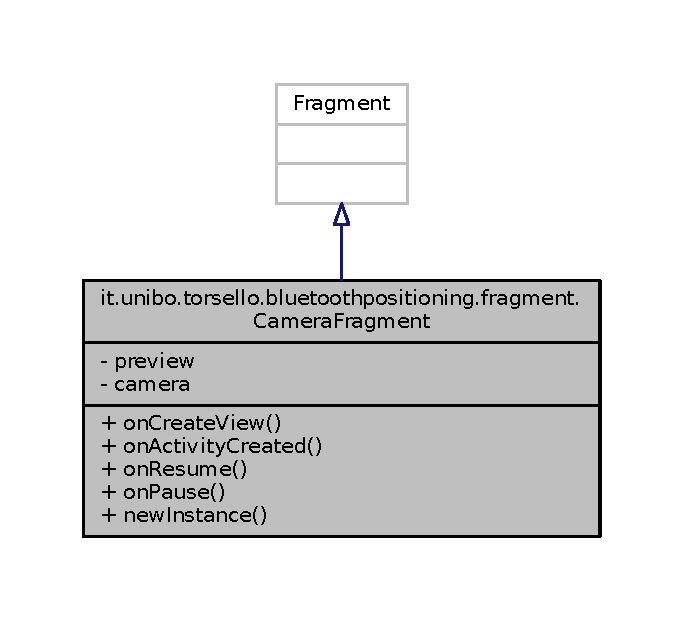
\includegraphics[width=328pt]{classit_1_1unibo_1_1torsello_1_1bluetoothpositioning_1_1fragment_1_1CameraFragment__inherit__graph}
\end{center}
\end{figure}


Diagramma di collaborazione per it.\+unibo.\+torsello.\+bluetoothpositioning.\+fragment.\+Camera\+Fragment\+:
\nopagebreak
\begin{figure}[H]
\begin{center}
\leavevmode
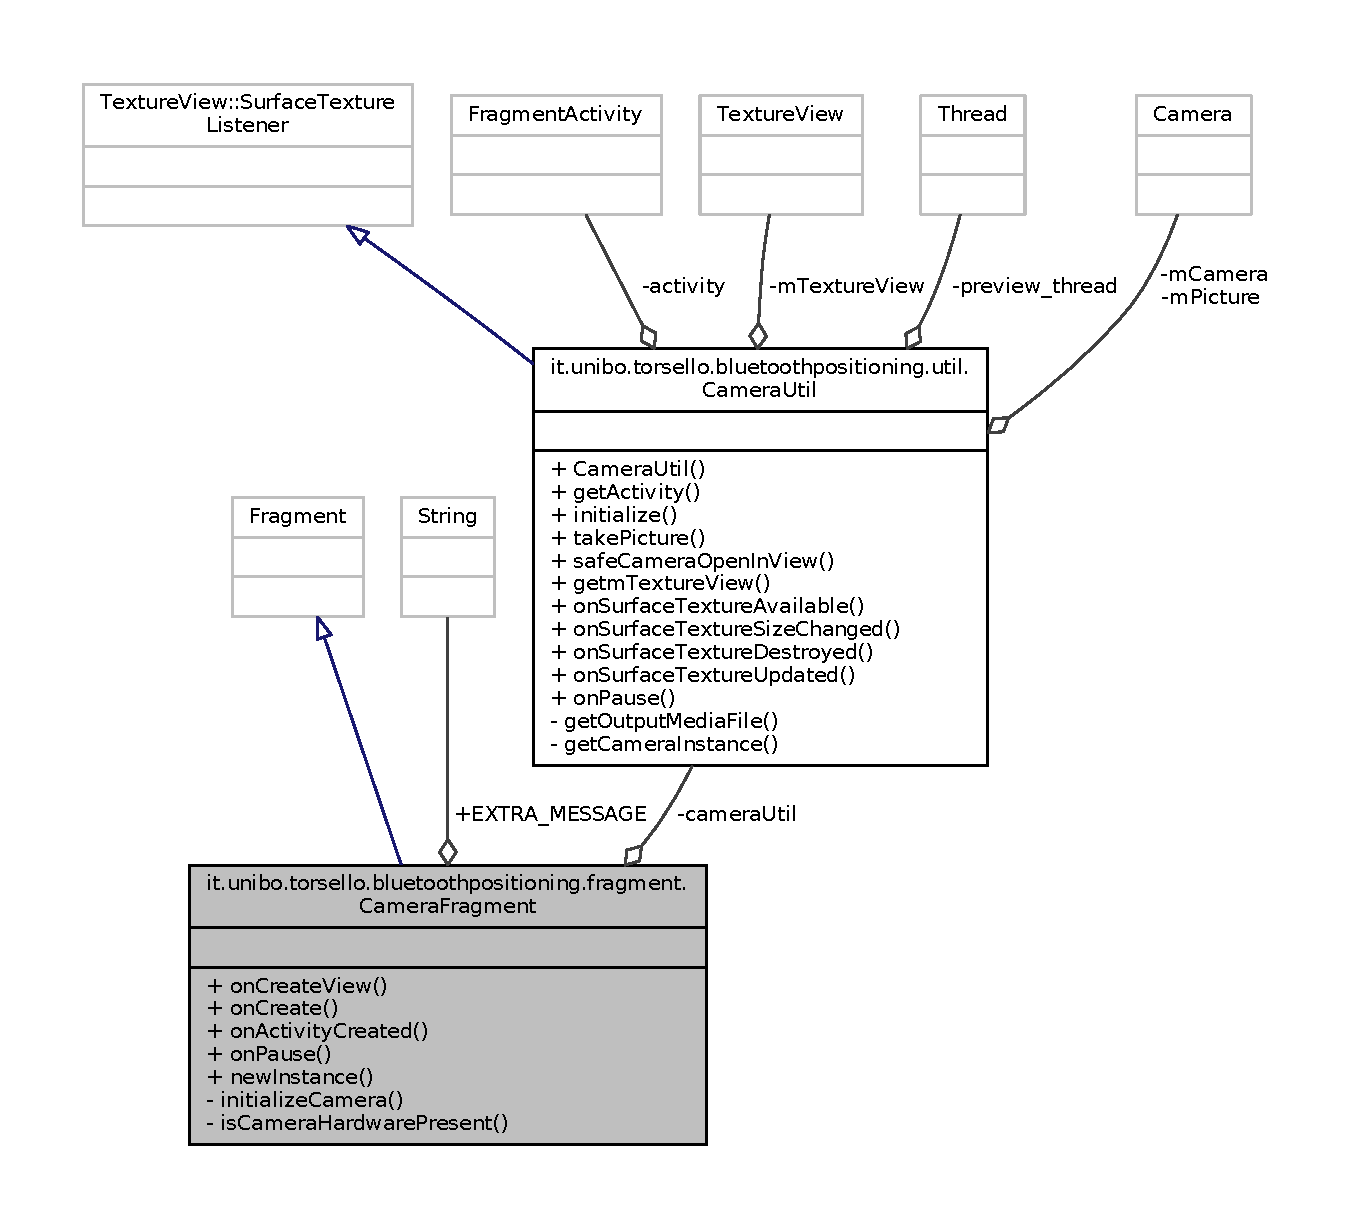
\includegraphics[width=350pt]{classit_1_1unibo_1_1torsello_1_1bluetoothpositioning_1_1fragment_1_1CameraFragment__coll__graph}
\end{center}
\end{figure}
\subsubsection*{Membri pubblici}
\begin{DoxyCompactItemize}
\item 
View \hyperlink{classit_1_1unibo_1_1torsello_1_1bluetoothpositioning_1_1fragment_1_1CameraFragment_a3a80f360922bd6a8c749cda2a09c64cf_a3a80f360922bd6a8c749cda2a09c64cf}{on\+Create\+View} (Layout\+Inflater inflater, View\+Group container, Bundle saved\+Instance\+State)
\item 
void \hyperlink{classit_1_1unibo_1_1torsello_1_1bluetoothpositioning_1_1fragment_1_1CameraFragment_a3af6cb206d2194e7d580cf511a97d6f1_a3af6cb206d2194e7d580cf511a97d6f1}{on\+Activity\+Created} (@Nullable Bundle saved\+Instance\+State)
\item 
void \hyperlink{classit_1_1unibo_1_1torsello_1_1bluetoothpositioning_1_1fragment_1_1CameraFragment_a8981ef6a92682639b28336a018bf1475_a8981ef6a92682639b28336a018bf1475}{on\+Resume} ()
\item 
void \hyperlink{classit_1_1unibo_1_1torsello_1_1bluetoothpositioning_1_1fragment_1_1CameraFragment_a3fb58eb9f1f5a3e516b9b21aa3e1e43d_a3fb58eb9f1f5a3e516b9b21aa3e1e43d}{on\+Pause} ()
\end{DoxyCompactItemize}
\subsubsection*{Membri pubblici statici}
\begin{DoxyCompactItemize}
\item 
static \hyperlink{classit_1_1unibo_1_1torsello_1_1bluetoothpositioning_1_1fragment_1_1CameraFragment}{Camera\+Fragment} \hyperlink{classit_1_1unibo_1_1torsello_1_1bluetoothpositioning_1_1fragment_1_1CameraFragment_a06506c839e3206fbe082ab705cb627b5_a06506c839e3206fbe082ab705cb627b5}{new\+Instance} ()
\end{DoxyCompactItemize}
\subsubsection*{Attributi con visibilità di package}
\begin{DoxyCompactItemize}
\item 
\hyperlink{classit_1_1unibo_1_1torsello_1_1bluetoothpositioning_1_1util_1_1CameraPreviewUtil}{Camera\+Preview\+Util} \hyperlink{classit_1_1unibo_1_1torsello_1_1bluetoothpositioning_1_1fragment_1_1CameraFragment_af14f8f1e4107c9a9063cf70d1fbb5bb5_af14f8f1e4107c9a9063cf70d1fbb5bb5}{preview}
\item 
Camera \hyperlink{classit_1_1unibo_1_1torsello_1_1bluetoothpositioning_1_1fragment_1_1CameraFragment_a70e1c67d2b127530751de08cb289b4c3_a70e1c67d2b127530751de08cb289b4c3}{camera}
\end{DoxyCompactItemize}


\subsubsection{Descrizione dettagliata}
Created by Federico Torsello. \href{mailto:federico.torsello@studio.unibo.it}{\tt federico.\+torsello@studio.\+unibo.\+it} 

\subsubsection{Documentazione delle funzioni membro}
\hypertarget{classit_1_1unibo_1_1torsello_1_1bluetoothpositioning_1_1fragment_1_1CameraFragment_a06506c839e3206fbe082ab705cb627b5_a06506c839e3206fbe082ab705cb627b5}{}\label{classit_1_1unibo_1_1torsello_1_1bluetoothpositioning_1_1fragment_1_1CameraFragment_a06506c839e3206fbe082ab705cb627b5_a06506c839e3206fbe082ab705cb627b5} 
\index{it\+::unibo\+::torsello\+::bluetoothpositioning\+::fragment\+::\+Camera\+Fragment@{it\+::unibo\+::torsello\+::bluetoothpositioning\+::fragment\+::\+Camera\+Fragment}!new\+Instance@{new\+Instance}}
\index{new\+Instance@{new\+Instance}!it\+::unibo\+::torsello\+::bluetoothpositioning\+::fragment\+::\+Camera\+Fragment@{it\+::unibo\+::torsello\+::bluetoothpositioning\+::fragment\+::\+Camera\+Fragment}}
\paragraph{\texorpdfstring{new\+Instance()}{newInstance()}}
{\footnotesize\ttfamily static \hyperlink{classit_1_1unibo_1_1torsello_1_1bluetoothpositioning_1_1fragment_1_1CameraFragment}{Camera\+Fragment} it.\+unibo.\+torsello.\+bluetoothpositioning.\+fragment.\+Camera\+Fragment.\+new\+Instance (\begin{DoxyParamCaption}{ }\end{DoxyParamCaption})\hspace{0.3cm}{\ttfamily [static]}}


\begin{DoxyCode}
25                                                \{
26         \textcolor{keywordflow}{return} \textcolor{keyword}{new} CameraFragment();
27     \}
\end{DoxyCode}
\hypertarget{classit_1_1unibo_1_1torsello_1_1bluetoothpositioning_1_1fragment_1_1CameraFragment_a3af6cb206d2194e7d580cf511a97d6f1_a3af6cb206d2194e7d580cf511a97d6f1}{}\label{classit_1_1unibo_1_1torsello_1_1bluetoothpositioning_1_1fragment_1_1CameraFragment_a3af6cb206d2194e7d580cf511a97d6f1_a3af6cb206d2194e7d580cf511a97d6f1} 
\index{it\+::unibo\+::torsello\+::bluetoothpositioning\+::fragment\+::\+Camera\+Fragment@{it\+::unibo\+::torsello\+::bluetoothpositioning\+::fragment\+::\+Camera\+Fragment}!on\+Activity\+Created@{on\+Activity\+Created}}
\index{on\+Activity\+Created@{on\+Activity\+Created}!it\+::unibo\+::torsello\+::bluetoothpositioning\+::fragment\+::\+Camera\+Fragment@{it\+::unibo\+::torsello\+::bluetoothpositioning\+::fragment\+::\+Camera\+Fragment}}
\paragraph{\texorpdfstring{on\+Activity\+Created()}{onActivityCreated()}}
{\footnotesize\ttfamily void it.\+unibo.\+torsello.\+bluetoothpositioning.\+fragment.\+Camera\+Fragment.\+on\+Activity\+Created (\begin{DoxyParamCaption}\item[{@Nullable Bundle}]{saved\+Instance\+State }\end{DoxyParamCaption})}


\begin{DoxyCode}
70                                                                        \{
71         super.onActivityCreated(savedInstanceState);
72 
73         getActivity().findViewById(R.id.fab\_camera).setOnClickListener(\textcolor{keyword}{new} View.OnClickListener() \{
74             @Override
75             \textcolor{keyword}{public} \textcolor{keywordtype}{void} onClick(View v) \{
76                 \hyperlink{classit_1_1unibo_1_1torsello_1_1bluetoothpositioning_1_1fragment_1_1CameraFragment_af14f8f1e4107c9a9063cf70d1fbb5bb5_af14f8f1e4107c9a9063cf70d1fbb5bb5}{preview}.\hyperlink{classit_1_1unibo_1_1torsello_1_1bluetoothpositioning_1_1util_1_1CameraPreviewUtil_a4f4ca8b7292c4e410f1f5aca3a53423a_a4f4ca8b7292c4e410f1f5aca3a53423a}{takePicture}();
77             \}
78         \});
79 
80     \}
\end{DoxyCode}
\hypertarget{classit_1_1unibo_1_1torsello_1_1bluetoothpositioning_1_1fragment_1_1CameraFragment_a3a80f360922bd6a8c749cda2a09c64cf_a3a80f360922bd6a8c749cda2a09c64cf}{}\label{classit_1_1unibo_1_1torsello_1_1bluetoothpositioning_1_1fragment_1_1CameraFragment_a3a80f360922bd6a8c749cda2a09c64cf_a3a80f360922bd6a8c749cda2a09c64cf} 
\index{it\+::unibo\+::torsello\+::bluetoothpositioning\+::fragment\+::\+Camera\+Fragment@{it\+::unibo\+::torsello\+::bluetoothpositioning\+::fragment\+::\+Camera\+Fragment}!on\+Create\+View@{on\+Create\+View}}
\index{on\+Create\+View@{on\+Create\+View}!it\+::unibo\+::torsello\+::bluetoothpositioning\+::fragment\+::\+Camera\+Fragment@{it\+::unibo\+::torsello\+::bluetoothpositioning\+::fragment\+::\+Camera\+Fragment}}
\paragraph{\texorpdfstring{on\+Create\+View()}{onCreateView()}}
{\footnotesize\ttfamily View it.\+unibo.\+torsello.\+bluetoothpositioning.\+fragment.\+Camera\+Fragment.\+on\+Create\+View (\begin{DoxyParamCaption}\item[{Layout\+Inflater}]{inflater,  }\item[{View\+Group}]{container,  }\item[{Bundle}]{saved\+Instance\+State }\end{DoxyParamCaption})}


\begin{DoxyCode}
30                                                                                                       \{
31 
32         View root = inflater.inflate(R.layout.fragment\_camera, container, \textcolor{keyword}{false});
33         \hyperlink{classit_1_1unibo_1_1torsello_1_1bluetoothpositioning_1_1fragment_1_1CameraFragment_af14f8f1e4107c9a9063cf70d1fbb5bb5_af14f8f1e4107c9a9063cf70d1fbb5bb5}{preview} = \textcolor{keyword}{new} CameraPreviewUtil(getContext(), (SurfaceView) root.findViewById(R.id.
      surfaceView));
34         ((FrameLayout) root.findViewById(R.id.layout)).addView(\hyperlink{classit_1_1unibo_1_1torsello_1_1bluetoothpositioning_1_1fragment_1_1CameraFragment_af14f8f1e4107c9a9063cf70d1fbb5bb5_af14f8f1e4107c9a9063cf70d1fbb5bb5}{preview});
35         \hyperlink{classit_1_1unibo_1_1torsello_1_1bluetoothpositioning_1_1fragment_1_1CameraFragment_af14f8f1e4107c9a9063cf70d1fbb5bb5_af14f8f1e4107c9a9063cf70d1fbb5bb5}{preview}.setKeepScreenOn(\textcolor{keyword}{true});
36         \hyperlink{classit_1_1unibo_1_1torsello_1_1bluetoothpositioning_1_1fragment_1_1CameraFragment_af14f8f1e4107c9a9063cf70d1fbb5bb5_af14f8f1e4107c9a9063cf70d1fbb5bb5}{preview}.setOnClickListener(\textcolor{keyword}{new} OnClickListener() \{
37 
38             @Override
39             \textcolor{keyword}{public} \textcolor{keywordtype}{void} onClick(View arg0) \{
40 \textcolor{comment}{//                preview.takePicture();}
41                 \hyperlink{classit_1_1unibo_1_1torsello_1_1bluetoothpositioning_1_1fragment_1_1CameraFragment_a70e1c67d2b127530751de08cb289b4c3_a70e1c67d2b127530751de08cb289b4c3}{camera}.autoFocus(\textcolor{keyword}{new} Camera.AutoFocusCallback() \{
42                     @Override
43                     \textcolor{keyword}{public} \textcolor{keywordtype}{void} onAutoFocus(\textcolor{keywordtype}{boolean} success, Camera arg1) \{
44 \textcolor{comment}{//                        if (success) \{}
45 \textcolor{comment}{//                            preview.takePicture();}
46 \textcolor{comment}{//                        \}}
47                     \}
48                 \});
49             \}
50         \});
51         \hyperlink{classit_1_1unibo_1_1torsello_1_1bluetoothpositioning_1_1fragment_1_1CameraFragment_af14f8f1e4107c9a9063cf70d1fbb5bb5_af14f8f1e4107c9a9063cf70d1fbb5bb5}{preview}.setOnLongClickListener(\textcolor{keyword}{new} View.OnLongClickListener() \{
52             @Override
53             \textcolor{keyword}{public} \textcolor{keywordtype}{boolean} onLongClick(View arg0) \{
54 
55                 \hyperlink{classit_1_1unibo_1_1torsello_1_1bluetoothpositioning_1_1fragment_1_1CameraFragment_a70e1c67d2b127530751de08cb289b4c3_a70e1c67d2b127530751de08cb289b4c3}{camera}.autoFocus(\textcolor{keyword}{new} Camera.AutoFocusCallback() \{
56                     @Override
57                     \textcolor{keyword}{public} \textcolor{keywordtype}{void} onAutoFocus(\textcolor{keywordtype}{boolean} success, Camera arg1) \{
58 \textcolor{comment}{//                        if (success) \{}
59 \textcolor{comment}{//                            preview.takePicture();}
60 \textcolor{comment}{//                        \}}
61                     \}
62                 \});
63                 \textcolor{keywordflow}{return} \textcolor{keyword}{true};
64             \}
65         \});
66         \textcolor{keywordflow}{return} root;
67     \}
\end{DoxyCode}
\hypertarget{classit_1_1unibo_1_1torsello_1_1bluetoothpositioning_1_1fragment_1_1CameraFragment_a3fb58eb9f1f5a3e516b9b21aa3e1e43d_a3fb58eb9f1f5a3e516b9b21aa3e1e43d}{}\label{classit_1_1unibo_1_1torsello_1_1bluetoothpositioning_1_1fragment_1_1CameraFragment_a3fb58eb9f1f5a3e516b9b21aa3e1e43d_a3fb58eb9f1f5a3e516b9b21aa3e1e43d} 
\index{it\+::unibo\+::torsello\+::bluetoothpositioning\+::fragment\+::\+Camera\+Fragment@{it\+::unibo\+::torsello\+::bluetoothpositioning\+::fragment\+::\+Camera\+Fragment}!on\+Pause@{on\+Pause}}
\index{on\+Pause@{on\+Pause}!it\+::unibo\+::torsello\+::bluetoothpositioning\+::fragment\+::\+Camera\+Fragment@{it\+::unibo\+::torsello\+::bluetoothpositioning\+::fragment\+::\+Camera\+Fragment}}
\paragraph{\texorpdfstring{on\+Pause()}{onPause()}}
{\footnotesize\ttfamily void it.\+unibo.\+torsello.\+bluetoothpositioning.\+fragment.\+Camera\+Fragment.\+on\+Pause (\begin{DoxyParamCaption}{ }\end{DoxyParamCaption})}


\begin{DoxyCode}
90                           \{
91         \hyperlink{classit_1_1unibo_1_1torsello_1_1bluetoothpositioning_1_1fragment_1_1CameraFragment_af14f8f1e4107c9a9063cf70d1fbb5bb5_af14f8f1e4107c9a9063cf70d1fbb5bb5}{preview}.\hyperlink{classit_1_1unibo_1_1torsello_1_1bluetoothpositioning_1_1util_1_1CameraPreviewUtil_a69da006b39dff168a1cd185c5aa886f8_a69da006b39dff168a1cd185c5aa886f8}{onPause}();
92         super.onPause();
93     \}
\end{DoxyCode}
\hypertarget{classit_1_1unibo_1_1torsello_1_1bluetoothpositioning_1_1fragment_1_1CameraFragment_a8981ef6a92682639b28336a018bf1475_a8981ef6a92682639b28336a018bf1475}{}\label{classit_1_1unibo_1_1torsello_1_1bluetoothpositioning_1_1fragment_1_1CameraFragment_a8981ef6a92682639b28336a018bf1475_a8981ef6a92682639b28336a018bf1475} 
\index{it\+::unibo\+::torsello\+::bluetoothpositioning\+::fragment\+::\+Camera\+Fragment@{it\+::unibo\+::torsello\+::bluetoothpositioning\+::fragment\+::\+Camera\+Fragment}!on\+Resume@{on\+Resume}}
\index{on\+Resume@{on\+Resume}!it\+::unibo\+::torsello\+::bluetoothpositioning\+::fragment\+::\+Camera\+Fragment@{it\+::unibo\+::torsello\+::bluetoothpositioning\+::fragment\+::\+Camera\+Fragment}}
\paragraph{\texorpdfstring{on\+Resume()}{onResume()}}
{\footnotesize\ttfamily void it.\+unibo.\+torsello.\+bluetoothpositioning.\+fragment.\+Camera\+Fragment.\+on\+Resume (\begin{DoxyParamCaption}{ }\end{DoxyParamCaption})}


\begin{DoxyCode}
83                            \{
84         super.onResume();
85         \hyperlink{classit_1_1unibo_1_1torsello_1_1bluetoothpositioning_1_1fragment_1_1CameraFragment_af14f8f1e4107c9a9063cf70d1fbb5bb5_af14f8f1e4107c9a9063cf70d1fbb5bb5}{preview}.\hyperlink{classit_1_1unibo_1_1torsello_1_1bluetoothpositioning_1_1util_1_1CameraPreviewUtil_acc49f348e381371fcad9d428ea4a15ca_acc49f348e381371fcad9d428ea4a15ca}{setCamera}(getActivity());
86         \hyperlink{classit_1_1unibo_1_1torsello_1_1bluetoothpositioning_1_1fragment_1_1CameraFragment_a70e1c67d2b127530751de08cb289b4c3_a70e1c67d2b127530751de08cb289b4c3}{camera} = \hyperlink{classit_1_1unibo_1_1torsello_1_1bluetoothpositioning_1_1fragment_1_1CameraFragment_af14f8f1e4107c9a9063cf70d1fbb5bb5_af14f8f1e4107c9a9063cf70d1fbb5bb5}{preview}.\hyperlink{classit_1_1unibo_1_1torsello_1_1bluetoothpositioning_1_1util_1_1CameraPreviewUtil_a24b83bd2a152f8f12824ccf190a90369_a24b83bd2a152f8f12824ccf190a90369}{getCamera}();
87     \}
\end{DoxyCode}


\subsubsection{Documentazione dei membri dato}
\hypertarget{classit_1_1unibo_1_1torsello_1_1bluetoothpositioning_1_1fragment_1_1CameraFragment_a70e1c67d2b127530751de08cb289b4c3_a70e1c67d2b127530751de08cb289b4c3}{}\label{classit_1_1unibo_1_1torsello_1_1bluetoothpositioning_1_1fragment_1_1CameraFragment_a70e1c67d2b127530751de08cb289b4c3_a70e1c67d2b127530751de08cb289b4c3} 
\index{it\+::unibo\+::torsello\+::bluetoothpositioning\+::fragment\+::\+Camera\+Fragment@{it\+::unibo\+::torsello\+::bluetoothpositioning\+::fragment\+::\+Camera\+Fragment}!camera@{camera}}
\index{camera@{camera}!it\+::unibo\+::torsello\+::bluetoothpositioning\+::fragment\+::\+Camera\+Fragment@{it\+::unibo\+::torsello\+::bluetoothpositioning\+::fragment\+::\+Camera\+Fragment}}
\paragraph{\texorpdfstring{camera}{camera}}
{\footnotesize\ttfamily Camera it.\+unibo.\+torsello.\+bluetoothpositioning.\+fragment.\+Camera\+Fragment.\+camera\hspace{0.3cm}{\ttfamily [package]}}

\hypertarget{classit_1_1unibo_1_1torsello_1_1bluetoothpositioning_1_1fragment_1_1CameraFragment_af14f8f1e4107c9a9063cf70d1fbb5bb5_af14f8f1e4107c9a9063cf70d1fbb5bb5}{}\label{classit_1_1unibo_1_1torsello_1_1bluetoothpositioning_1_1fragment_1_1CameraFragment_af14f8f1e4107c9a9063cf70d1fbb5bb5_af14f8f1e4107c9a9063cf70d1fbb5bb5} 
\index{it\+::unibo\+::torsello\+::bluetoothpositioning\+::fragment\+::\+Camera\+Fragment@{it\+::unibo\+::torsello\+::bluetoothpositioning\+::fragment\+::\+Camera\+Fragment}!preview@{preview}}
\index{preview@{preview}!it\+::unibo\+::torsello\+::bluetoothpositioning\+::fragment\+::\+Camera\+Fragment@{it\+::unibo\+::torsello\+::bluetoothpositioning\+::fragment\+::\+Camera\+Fragment}}
\paragraph{\texorpdfstring{preview}{preview}}
{\footnotesize\ttfamily \hyperlink{classit_1_1unibo_1_1torsello_1_1bluetoothpositioning_1_1util_1_1CameraPreviewUtil}{Camera\+Preview\+Util} it.\+unibo.\+torsello.\+bluetoothpositioning.\+fragment.\+Camera\+Fragment.\+preview\hspace{0.3cm}{\ttfamily [package]}}



La documentazione per questa classe è stata generata a partire dal seguente file\+:\begin{DoxyCompactItemize}
\item 
\hyperlink{CameraFragment_8java}{Camera\+Fragment.\+java}\end{DoxyCompactItemize}

\hypertarget{classit_1_1unibo_1_1torsello_1_1bluetoothpositioning_1_1util_1_1CameraUtil}{}\subsection{Riferimenti per la classe it.\+unibo.\+torsello.\+bluetoothpositioning.\+util.\+Camera\+Util}
\label{classit_1_1unibo_1_1torsello_1_1bluetoothpositioning_1_1util_1_1CameraUtil}\index{it.\+unibo.\+torsello.\+bluetoothpositioning.\+util.\+Camera\+Util@{it.\+unibo.\+torsello.\+bluetoothpositioning.\+util.\+Camera\+Util}}


Diagramma delle classi per it.\+unibo.\+torsello.\+bluetoothpositioning.\+util.\+Camera\+Util
\nopagebreak
\begin{figure}[H]
\begin{center}
\leavevmode
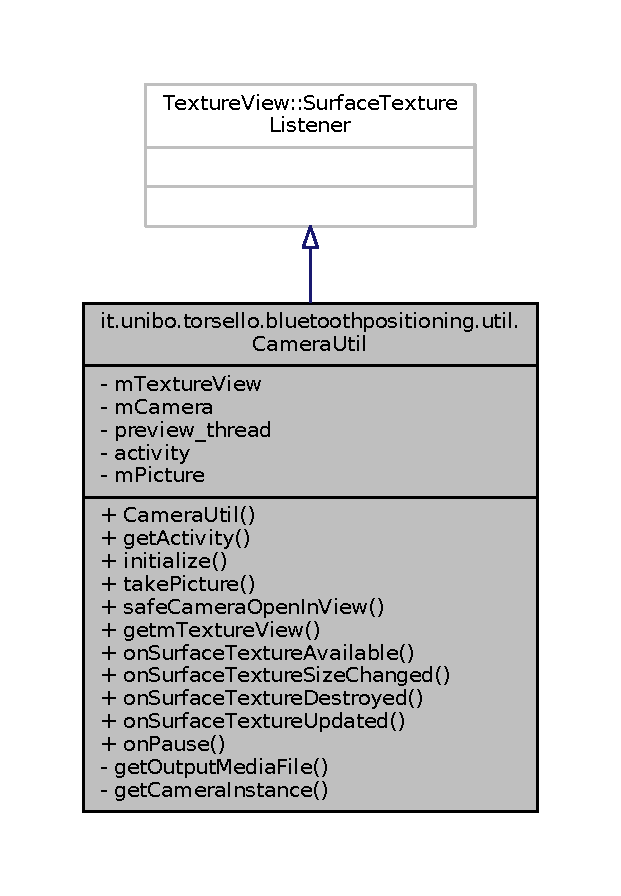
\includegraphics[width=298pt]{classit_1_1unibo_1_1torsello_1_1bluetoothpositioning_1_1util_1_1CameraUtil__inherit__graph}
\end{center}
\end{figure}


Diagramma di collaborazione per it.\+unibo.\+torsello.\+bluetoothpositioning.\+util.\+Camera\+Util\+:
\nopagebreak
\begin{figure}[H]
\begin{center}
\leavevmode
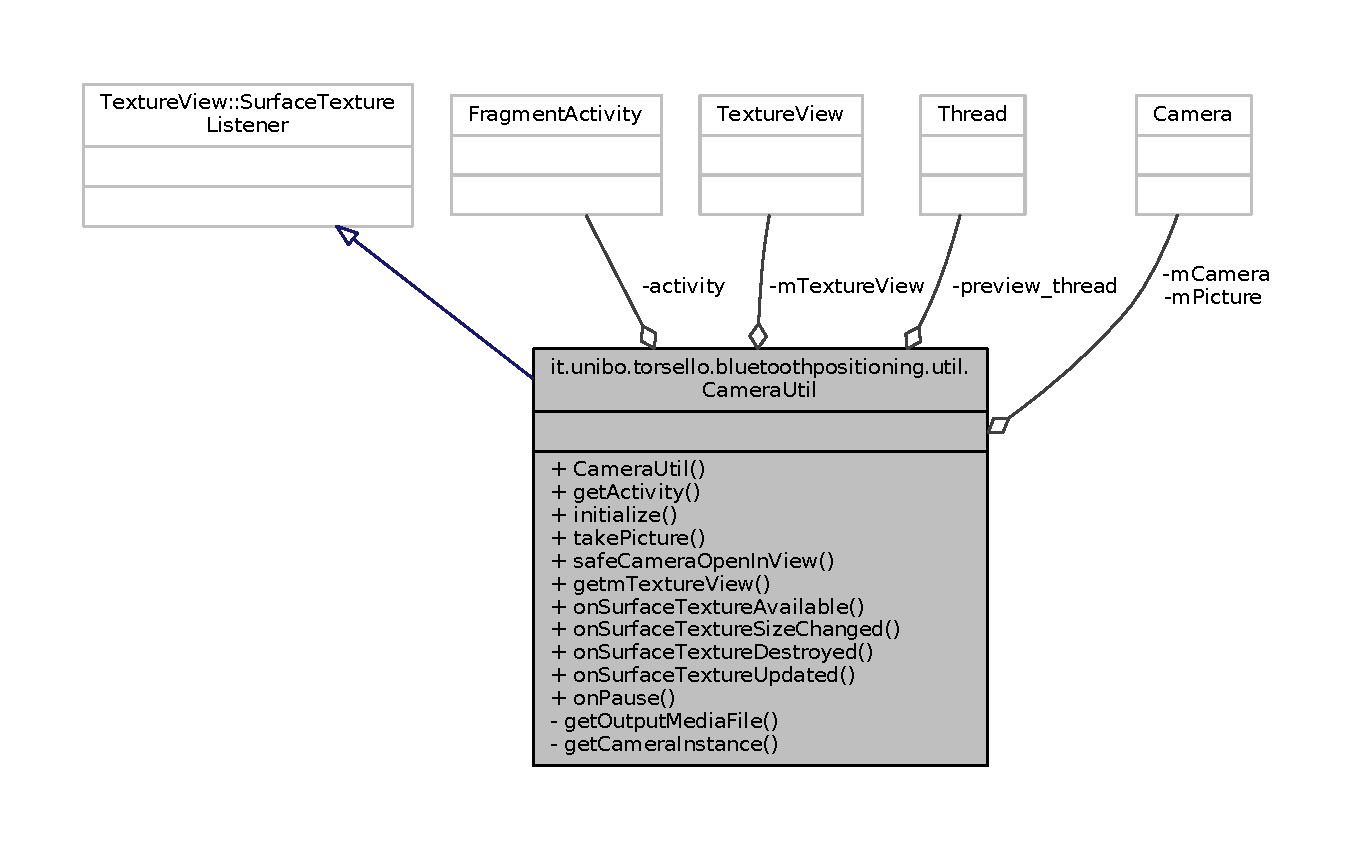
\includegraphics[width=350pt]{classit_1_1unibo_1_1torsello_1_1bluetoothpositioning_1_1util_1_1CameraUtil__coll__graph}
\end{center}
\end{figure}
\subsubsection*{Membri pubblici}
\begin{DoxyCompactItemize}
\item 
\hyperlink{classit_1_1unibo_1_1torsello_1_1bluetoothpositioning_1_1util_1_1CameraUtil_a0d016ada31702f7069b01740ae3bf22f_a0d016ada31702f7069b01740ae3bf22f}{Camera\+Util} (Fragment\+Activity fragment\+Activity)
\item 
Fragment\+Activity \hyperlink{classit_1_1unibo_1_1torsello_1_1bluetoothpositioning_1_1util_1_1CameraUtil_ad49c34169e8267bb8f841d27f0d5804b_ad49c34169e8267bb8f841d27f0d5804b}{get\+Activity} ()
\item 
void \hyperlink{classit_1_1unibo_1_1torsello_1_1bluetoothpositioning_1_1util_1_1CameraUtil_ae88de176ab49ea6eafa5864701ecc748_ae88de176ab49ea6eafa5864701ecc748}{initialize} ()
\item 
void \hyperlink{classit_1_1unibo_1_1torsello_1_1bluetoothpositioning_1_1util_1_1CameraUtil_a4223fa54dcdd332f394f9d4b6395ec79_a4223fa54dcdd332f394f9d4b6395ec79}{take\+Picture} ()
\item 
void \hyperlink{classit_1_1unibo_1_1torsello_1_1bluetoothpositioning_1_1util_1_1CameraUtil_af983e424981a3991fd9d241217328bc8_af983e424981a3991fd9d241217328bc8}{safe\+Camera\+Open\+In\+View} (Surface\+Texture surface)
\item 
Texture\+View \hyperlink{classit_1_1unibo_1_1torsello_1_1bluetoothpositioning_1_1util_1_1CameraUtil_a5465cd771c9607dce53409cba1e4e1d9_a5465cd771c9607dce53409cba1e4e1d9}{getm\+Texture\+View} ()
\item 
void \hyperlink{classit_1_1unibo_1_1torsello_1_1bluetoothpositioning_1_1util_1_1CameraUtil_ae57c993ba40e5d0a601e246abc67b919_ae57c993ba40e5d0a601e246abc67b919}{on\+Surface\+Texture\+Available} (final Surface\+Texture surface, int width, int height)
\item 
void \hyperlink{classit_1_1unibo_1_1torsello_1_1bluetoothpositioning_1_1util_1_1CameraUtil_ae1a6cb9d0f4b5ea28321088152126b79_ae1a6cb9d0f4b5ea28321088152126b79}{on\+Surface\+Texture\+Size\+Changed} (Surface\+Texture surface, int width, int height)
\item 
boolean \hyperlink{classit_1_1unibo_1_1torsello_1_1bluetoothpositioning_1_1util_1_1CameraUtil_a0189f59aac3827e05165a29cc8658d95_a0189f59aac3827e05165a29cc8658d95}{on\+Surface\+Texture\+Destroyed} (Surface\+Texture surface)
\item 
void \hyperlink{classit_1_1unibo_1_1torsello_1_1bluetoothpositioning_1_1util_1_1CameraUtil_aede93d13d58ef68302980917ac06612a_aede93d13d58ef68302980917ac06612a}{on\+Surface\+Texture\+Updated} (Surface\+Texture surface)
\item 
void \hyperlink{classit_1_1unibo_1_1torsello_1_1bluetoothpositioning_1_1util_1_1CameraUtil_a1ebe095e57994dfb73a9ead49d72017e_a1ebe095e57994dfb73a9ead49d72017e}{on\+Pause} ()
\end{DoxyCompactItemize}
\subsubsection*{Membri privati}
\begin{DoxyCompactItemize}
\item 
File \hyperlink{classit_1_1unibo_1_1torsello_1_1bluetoothpositioning_1_1util_1_1CameraUtil_acef4209a5ff8034ddd3adab34761fe98_acef4209a5ff8034ddd3adab34761fe98}{get\+Output\+Media\+File} ()
\end{DoxyCompactItemize}
\subsubsection*{Membri privati statici}
\begin{DoxyCompactItemize}
\item 
static Camera \hyperlink{classit_1_1unibo_1_1torsello_1_1bluetoothpositioning_1_1util_1_1CameraUtil_afd1bf5fd806ad3dd71463e2f0084b619_afd1bf5fd806ad3dd71463e2f0084b619}{get\+Camera\+Instance} ()
\end{DoxyCompactItemize}
\subsubsection*{Attributi privati}
\begin{DoxyCompactItemize}
\item 
Texture\+View \hyperlink{classit_1_1unibo_1_1torsello_1_1bluetoothpositioning_1_1util_1_1CameraUtil_a4fb9e02d00c0a61cb6b8992e085cf374_a4fb9e02d00c0a61cb6b8992e085cf374}{m\+Texture\+View}
\item 
Camera \hyperlink{classit_1_1unibo_1_1torsello_1_1bluetoothpositioning_1_1util_1_1CameraUtil_ac3d03bd30262a62e27b80e7bab97b40b_ac3d03bd30262a62e27b80e7bab97b40b}{m\+Camera}
\item 
Thread \hyperlink{classit_1_1unibo_1_1torsello_1_1bluetoothpositioning_1_1util_1_1CameraUtil_a49f1624f6df81b6a7604b5928c17d443_a49f1624f6df81b6a7604b5928c17d443}{preview\+\_\+thread}
\item 
Fragment\+Activity \hyperlink{classit_1_1unibo_1_1torsello_1_1bluetoothpositioning_1_1util_1_1CameraUtil_a06e6b6842aa57e9e9db83a88b4aa3f25_a06e6b6842aa57e9e9db83a88b4aa3f25}{activity}
\item 
Camera.\+Picture\+Callback \hyperlink{classit_1_1unibo_1_1torsello_1_1bluetoothpositioning_1_1util_1_1CameraUtil_a1f456d8724b3f804be64512d8fcaef37_a1f456d8724b3f804be64512d8fcaef37}{m\+Picture}
\end{DoxyCompactItemize}


\subsubsection{Descrizione dettagliata}
Created by Federico Torsello. \href{mailto:federico.torsello@studio.unibo.it}{\tt federico.\+torsello@studio.\+unibo.\+it} 

\subsubsection{Documentazione dei costruttori e dei distruttori}
\hypertarget{classit_1_1unibo_1_1torsello_1_1bluetoothpositioning_1_1util_1_1CameraUtil_a0d016ada31702f7069b01740ae3bf22f_a0d016ada31702f7069b01740ae3bf22f}{}\label{classit_1_1unibo_1_1torsello_1_1bluetoothpositioning_1_1util_1_1CameraUtil_a0d016ada31702f7069b01740ae3bf22f_a0d016ada31702f7069b01740ae3bf22f} 
\index{it\+::unibo\+::torsello\+::bluetoothpositioning\+::util\+::\+Camera\+Util@{it\+::unibo\+::torsello\+::bluetoothpositioning\+::util\+::\+Camera\+Util}!Camera\+Util@{Camera\+Util}}
\index{Camera\+Util@{Camera\+Util}!it\+::unibo\+::torsello\+::bluetoothpositioning\+::util\+::\+Camera\+Util@{it\+::unibo\+::torsello\+::bluetoothpositioning\+::util\+::\+Camera\+Util}}
\paragraph{\texorpdfstring{Camera\+Util()}{CameraUtil()}}
{\footnotesize\ttfamily it.\+unibo.\+torsello.\+bluetoothpositioning.\+util.\+Camera\+Util.\+Camera\+Util (\begin{DoxyParamCaption}\item[{Fragment\+Activity}]{fragment\+Activity }\end{DoxyParamCaption})}


\begin{DoxyCode}
52                                                          \{
53         this.\hyperlink{classit_1_1unibo_1_1torsello_1_1bluetoothpositioning_1_1util_1_1CameraUtil_a06e6b6842aa57e9e9db83a88b4aa3f25_a06e6b6842aa57e9e9db83a88b4aa3f25}{activity} = fragmentActivity;
54     \}
\end{DoxyCode}


\subsubsection{Documentazione delle funzioni membro}
\hypertarget{classit_1_1unibo_1_1torsello_1_1bluetoothpositioning_1_1util_1_1CameraUtil_ad49c34169e8267bb8f841d27f0d5804b_ad49c34169e8267bb8f841d27f0d5804b}{}\label{classit_1_1unibo_1_1torsello_1_1bluetoothpositioning_1_1util_1_1CameraUtil_ad49c34169e8267bb8f841d27f0d5804b_ad49c34169e8267bb8f841d27f0d5804b} 
\index{it\+::unibo\+::torsello\+::bluetoothpositioning\+::util\+::\+Camera\+Util@{it\+::unibo\+::torsello\+::bluetoothpositioning\+::util\+::\+Camera\+Util}!get\+Activity@{get\+Activity}}
\index{get\+Activity@{get\+Activity}!it\+::unibo\+::torsello\+::bluetoothpositioning\+::util\+::\+Camera\+Util@{it\+::unibo\+::torsello\+::bluetoothpositioning\+::util\+::\+Camera\+Util}}
\paragraph{\texorpdfstring{get\+Activity()}{getActivity()}}
{\footnotesize\ttfamily Fragment\+Activity it.\+unibo.\+torsello.\+bluetoothpositioning.\+util.\+Camera\+Util.\+get\+Activity (\begin{DoxyParamCaption}{ }\end{DoxyParamCaption})}


\begin{DoxyCode}
56                                           \{
57         \textcolor{keywordflow}{return} \hyperlink{classit_1_1unibo_1_1torsello_1_1bluetoothpositioning_1_1util_1_1CameraUtil_a06e6b6842aa57e9e9db83a88b4aa3f25_a06e6b6842aa57e9e9db83a88b4aa3f25}{activity};
58     \}
\end{DoxyCode}
\hypertarget{classit_1_1unibo_1_1torsello_1_1bluetoothpositioning_1_1util_1_1CameraUtil_afd1bf5fd806ad3dd71463e2f0084b619_afd1bf5fd806ad3dd71463e2f0084b619}{}\label{classit_1_1unibo_1_1torsello_1_1bluetoothpositioning_1_1util_1_1CameraUtil_afd1bf5fd806ad3dd71463e2f0084b619_afd1bf5fd806ad3dd71463e2f0084b619} 
\index{it\+::unibo\+::torsello\+::bluetoothpositioning\+::util\+::\+Camera\+Util@{it\+::unibo\+::torsello\+::bluetoothpositioning\+::util\+::\+Camera\+Util}!get\+Camera\+Instance@{get\+Camera\+Instance}}
\index{get\+Camera\+Instance@{get\+Camera\+Instance}!it\+::unibo\+::torsello\+::bluetoothpositioning\+::util\+::\+Camera\+Util@{it\+::unibo\+::torsello\+::bluetoothpositioning\+::util\+::\+Camera\+Util}}
\paragraph{\texorpdfstring{get\+Camera\+Instance()}{getCameraInstance()}}
{\footnotesize\ttfamily static Camera it.\+unibo.\+torsello.\+bluetoothpositioning.\+util.\+Camera\+Util.\+get\+Camera\+Instance (\begin{DoxyParamCaption}{ }\end{DoxyParamCaption})\hspace{0.3cm}{\ttfamily [static]}, {\ttfamily [private]}}

A safe way to get an instance of the \hyperlink{classit_1_1unibo_1_1torsello_1_1bluetoothpositioning_1_1util_1_1CameraUtil}{Camera\+Util} object. 
\begin{DoxyCode}
63                                               \{
64 
65         Camera c = null;
66 
67         \textcolor{keywordflow}{try} \{
68             c = Camera.open(); \textcolor{comment}{// attempt to get a CameraUtil instance}
69         \} \textcolor{keywordflow}{catch} (RuntimeException e) \{
70             \textcolor{comment}{// CameraUtil is not available (in use or does not exist)}
71             e.getStackTrace();
72         \}
73 
74         \textcolor{keywordflow}{return} c; \textcolor{comment}{// returns null if camera is unavailable}
75     \}
\end{DoxyCode}
\hypertarget{classit_1_1unibo_1_1torsello_1_1bluetoothpositioning_1_1util_1_1CameraUtil_a5465cd771c9607dce53409cba1e4e1d9_a5465cd771c9607dce53409cba1e4e1d9}{}\label{classit_1_1unibo_1_1torsello_1_1bluetoothpositioning_1_1util_1_1CameraUtil_a5465cd771c9607dce53409cba1e4e1d9_a5465cd771c9607dce53409cba1e4e1d9} 
\index{it\+::unibo\+::torsello\+::bluetoothpositioning\+::util\+::\+Camera\+Util@{it\+::unibo\+::torsello\+::bluetoothpositioning\+::util\+::\+Camera\+Util}!getm\+Texture\+View@{getm\+Texture\+View}}
\index{getm\+Texture\+View@{getm\+Texture\+View}!it\+::unibo\+::torsello\+::bluetoothpositioning\+::util\+::\+Camera\+Util@{it\+::unibo\+::torsello\+::bluetoothpositioning\+::util\+::\+Camera\+Util}}
\paragraph{\texorpdfstring{getm\+Texture\+View()}{getmTextureView()}}
{\footnotesize\ttfamily Texture\+View it.\+unibo.\+torsello.\+bluetoothpositioning.\+util.\+Camera\+Util.\+getm\+Texture\+View (\begin{DoxyParamCaption}{ }\end{DoxyParamCaption})}


\begin{DoxyCode}
157                                          \{
158         \textcolor{keywordflow}{return} \hyperlink{classit_1_1unibo_1_1torsello_1_1bluetoothpositioning_1_1util_1_1CameraUtil_a4fb9e02d00c0a61cb6b8992e085cf374_a4fb9e02d00c0a61cb6b8992e085cf374}{mTextureView};
159     \}
\end{DoxyCode}
\hypertarget{classit_1_1unibo_1_1torsello_1_1bluetoothpositioning_1_1util_1_1CameraUtil_acef4209a5ff8034ddd3adab34761fe98_acef4209a5ff8034ddd3adab34761fe98}{}\label{classit_1_1unibo_1_1torsello_1_1bluetoothpositioning_1_1util_1_1CameraUtil_acef4209a5ff8034ddd3adab34761fe98_acef4209a5ff8034ddd3adab34761fe98} 
\index{it\+::unibo\+::torsello\+::bluetoothpositioning\+::util\+::\+Camera\+Util@{it\+::unibo\+::torsello\+::bluetoothpositioning\+::util\+::\+Camera\+Util}!get\+Output\+Media\+File@{get\+Output\+Media\+File}}
\index{get\+Output\+Media\+File@{get\+Output\+Media\+File}!it\+::unibo\+::torsello\+::bluetoothpositioning\+::util\+::\+Camera\+Util@{it\+::unibo\+::torsello\+::bluetoothpositioning\+::util\+::\+Camera\+Util}}
\paragraph{\texorpdfstring{get\+Output\+Media\+File()}{getOutputMediaFile()}}
{\footnotesize\ttfamily File it.\+unibo.\+torsello.\+bluetoothpositioning.\+util.\+Camera\+Util.\+get\+Output\+Media\+File (\begin{DoxyParamCaption}{ }\end{DoxyParamCaption})\hspace{0.3cm}{\ttfamily [private]}}

Used to return the camera File output.

\begin{DoxyReturn}{Restituisce}

\end{DoxyReturn}

\begin{DoxyCode}
128                                       \{
129 
130         File mediaStorageDir = \textcolor{keyword}{new} File(Environment.getExternalStoragePublicDirectory(
131                 Environment.DIRECTORY\_PICTURES), \hyperlink{classit_1_1unibo_1_1torsello_1_1bluetoothpositioning_1_1util_1_1CameraUtil_ad49c34169e8267bb8f841d27f0d5804b_ad49c34169e8267bb8f841d27f0d5804b}{getActivity}().getString(R.string.app\_name));
132 
133         \textcolor{keywordflow}{if} (!mediaStorageDir.exists()) \{
134             \textcolor{keywordflow}{if} (!mediaStorageDir.mkdirs()) \{
135                 Log.i(\textcolor{stringliteral}{"CameraUtil Guide"}, \textcolor{stringliteral}{"Required media storage does not exist"});
136                 \textcolor{keywordflow}{return} null;
137             \}
138         \}
139 
140         \textcolor{comment}{// Create a media file name}
141         String timeStamp = \textcolor{keyword}{new} SimpleDateFormat(\textcolor{stringliteral}{"yyyyMMdd\_HHmmss"}).format(\textcolor{keyword}{new} Date());
142         File mediaFile = \textcolor{keyword}{new} File(mediaStorageDir.getPath() + File.separator +
143                 \textcolor{stringliteral}{"IMG\_"} + timeStamp + \textcolor{stringliteral}{".jpg"});
144 
145         \textcolor{keyword}{new} AlertDialog.Builder(\hyperlink{classit_1_1unibo_1_1torsello_1_1bluetoothpositioning_1_1util_1_1CameraUtil_ad49c34169e8267bb8f841d27f0d5804b_ad49c34169e8267bb8f841d27f0d5804b}{getActivity}())
146                 .setTitle(\textcolor{stringliteral}{"Success!"})
147                 .setMessage(\textcolor{stringliteral}{"Your picture has been saved!"})
148                 .setPositiveButton(android.R.string.ok, \textcolor{keyword}{new} DialogInterface.OnClickListener() \{
149                     \textcolor{keyword}{public} \textcolor{keywordtype}{void} onClick(DialogInterface dialog, \textcolor{keywordtype}{int} \textcolor{keywordtype}{id}) \{
150                         dialog.dismiss();
151                     \}
152                 \}).show();
153 
154         \textcolor{keywordflow}{return} mediaFile;
155     \}
\end{DoxyCode}
\hypertarget{classit_1_1unibo_1_1torsello_1_1bluetoothpositioning_1_1util_1_1CameraUtil_ae88de176ab49ea6eafa5864701ecc748_ae88de176ab49ea6eafa5864701ecc748}{}\label{classit_1_1unibo_1_1torsello_1_1bluetoothpositioning_1_1util_1_1CameraUtil_ae88de176ab49ea6eafa5864701ecc748_ae88de176ab49ea6eafa5864701ecc748} 
\index{it\+::unibo\+::torsello\+::bluetoothpositioning\+::util\+::\+Camera\+Util@{it\+::unibo\+::torsello\+::bluetoothpositioning\+::util\+::\+Camera\+Util}!initialize@{initialize}}
\index{initialize@{initialize}!it\+::unibo\+::torsello\+::bluetoothpositioning\+::util\+::\+Camera\+Util@{it\+::unibo\+::torsello\+::bluetoothpositioning\+::util\+::\+Camera\+Util}}
\paragraph{\texorpdfstring{initialize()}{initialize()}}
{\footnotesize\ttfamily void it.\+unibo.\+torsello.\+bluetoothpositioning.\+util.\+Camera\+Util.\+initialize (\begin{DoxyParamCaption}{ }\end{DoxyParamCaption})}


\begin{DoxyCode}
77                              \{
78         \textcolor{keywordflow}{if} (\hyperlink{classit_1_1unibo_1_1torsello_1_1bluetoothpositioning_1_1util_1_1CameraUtil_ac3d03bd30262a62e27b80e7bab97b40b_ac3d03bd30262a62e27b80e7bab97b40b}{mCamera} == null) \{
79             \hyperlink{classit_1_1unibo_1_1torsello_1_1bluetoothpositioning_1_1util_1_1CameraUtil_ac3d03bd30262a62e27b80e7bab97b40b_ac3d03bd30262a62e27b80e7bab97b40b}{mCamera} = \hyperlink{classit_1_1unibo_1_1torsello_1_1bluetoothpositioning_1_1util_1_1CameraUtil_afd1bf5fd806ad3dd71463e2f0084b619_afd1bf5fd806ad3dd71463e2f0084b619}{getCameraInstance}();
80         \}
81 
82         \hyperlink{classit_1_1unibo_1_1torsello_1_1bluetoothpositioning_1_1util_1_1CameraUtil_a4fb9e02d00c0a61cb6b8992e085cf374_a4fb9e02d00c0a61cb6b8992e085cf374}{mTextureView} = \textcolor{keyword}{new} TextureView(\hyperlink{classit_1_1unibo_1_1torsello_1_1bluetoothpositioning_1_1util_1_1CameraUtil_ad49c34169e8267bb8f841d27f0d5804b_ad49c34169e8267bb8f841d27f0d5804b}{getActivity}());
83         \hyperlink{classit_1_1unibo_1_1torsello_1_1bluetoothpositioning_1_1util_1_1CameraUtil_a4fb9e02d00c0a61cb6b8992e085cf374_a4fb9e02d00c0a61cb6b8992e085cf374}{mTextureView}.setSurfaceTextureListener(\textcolor{keyword}{this});
84 
85     \}
\end{DoxyCode}
\hypertarget{classit_1_1unibo_1_1torsello_1_1bluetoothpositioning_1_1util_1_1CameraUtil_a1ebe095e57994dfb73a9ead49d72017e_a1ebe095e57994dfb73a9ead49d72017e}{}\label{classit_1_1unibo_1_1torsello_1_1bluetoothpositioning_1_1util_1_1CameraUtil_a1ebe095e57994dfb73a9ead49d72017e_a1ebe095e57994dfb73a9ead49d72017e} 
\index{it\+::unibo\+::torsello\+::bluetoothpositioning\+::util\+::\+Camera\+Util@{it\+::unibo\+::torsello\+::bluetoothpositioning\+::util\+::\+Camera\+Util}!on\+Pause@{on\+Pause}}
\index{on\+Pause@{on\+Pause}!it\+::unibo\+::torsello\+::bluetoothpositioning\+::util\+::\+Camera\+Util@{it\+::unibo\+::torsello\+::bluetoothpositioning\+::util\+::\+Camera\+Util}}
\paragraph{\texorpdfstring{on\+Pause()}{onPause()}}
{\footnotesize\ttfamily void it.\+unibo.\+torsello.\+bluetoothpositioning.\+util.\+Camera\+Util.\+on\+Pause (\begin{DoxyParamCaption}{ }\end{DoxyParamCaption})}


\begin{DoxyCode}
195                           \{
196         \textcolor{keywordflow}{if} (\hyperlink{classit_1_1unibo_1_1torsello_1_1bluetoothpositioning_1_1util_1_1CameraUtil_ac3d03bd30262a62e27b80e7bab97b40b_ac3d03bd30262a62e27b80e7bab97b40b}{mCamera} != null) \{
197             \textcolor{keywordflow}{if} (\hyperlink{classit_1_1unibo_1_1torsello_1_1bluetoothpositioning_1_1util_1_1CameraUtil_a49f1624f6df81b6a7604b5928c17d443_a49f1624f6df81b6a7604b5928c17d443}{preview\_thread} != null && !\hyperlink{classit_1_1unibo_1_1torsello_1_1bluetoothpositioning_1_1util_1_1CameraUtil_a49f1624f6df81b6a7604b5928c17d443_a49f1624f6df81b6a7604b5928c17d443}{preview\_thread}.isInterrupted()) \{
198                 \hyperlink{classit_1_1unibo_1_1torsello_1_1bluetoothpositioning_1_1util_1_1CameraUtil_a49f1624f6df81b6a7604b5928c17d443_a49f1624f6df81b6a7604b5928c17d443}{preview\_thread}.interrupt();
199             \}
200             \hyperlink{classit_1_1unibo_1_1torsello_1_1bluetoothpositioning_1_1util_1_1CameraUtil_ac3d03bd30262a62e27b80e7bab97b40b_ac3d03bd30262a62e27b80e7bab97b40b}{mCamera}.stopPreview();
201             \hyperlink{classit_1_1unibo_1_1torsello_1_1bluetoothpositioning_1_1util_1_1CameraUtil_ac3d03bd30262a62e27b80e7bab97b40b_ac3d03bd30262a62e27b80e7bab97b40b}{mCamera}.release();
202             \hyperlink{classit_1_1unibo_1_1torsello_1_1bluetoothpositioning_1_1util_1_1CameraUtil_ac3d03bd30262a62e27b80e7bab97b40b_ac3d03bd30262a62e27b80e7bab97b40b}{mCamera} = null;
203         \}
204     \}
\end{DoxyCode}
\hypertarget{classit_1_1unibo_1_1torsello_1_1bluetoothpositioning_1_1util_1_1CameraUtil_ae57c993ba40e5d0a601e246abc67b919_ae57c993ba40e5d0a601e246abc67b919}{}\label{classit_1_1unibo_1_1torsello_1_1bluetoothpositioning_1_1util_1_1CameraUtil_ae57c993ba40e5d0a601e246abc67b919_ae57c993ba40e5d0a601e246abc67b919} 
\index{it\+::unibo\+::torsello\+::bluetoothpositioning\+::util\+::\+Camera\+Util@{it\+::unibo\+::torsello\+::bluetoothpositioning\+::util\+::\+Camera\+Util}!on\+Surface\+Texture\+Available@{on\+Surface\+Texture\+Available}}
\index{on\+Surface\+Texture\+Available@{on\+Surface\+Texture\+Available}!it\+::unibo\+::torsello\+::bluetoothpositioning\+::util\+::\+Camera\+Util@{it\+::unibo\+::torsello\+::bluetoothpositioning\+::util\+::\+Camera\+Util}}
\paragraph{\texorpdfstring{on\+Surface\+Texture\+Available()}{onSurfaceTextureAvailable()}}
{\footnotesize\ttfamily void it.\+unibo.\+torsello.\+bluetoothpositioning.\+util.\+Camera\+Util.\+on\+Surface\+Texture\+Available (\begin{DoxyParamCaption}\item[{final Surface\+Texture}]{surface,  }\item[{int}]{width,  }\item[{int}]{height }\end{DoxyParamCaption})}


\begin{DoxyCode}
162                                                                                                \{
163 
164         \textcolor{keywordflow}{if} (surface == null) \{
165             \textcolor{comment}{// preview surface does not exist}
166             \textcolor{keywordflow}{return};
167         \}
168 
169         \textcolor{comment}{// Restart the camera preview.}
170         \hyperlink{classit_1_1unibo_1_1torsello_1_1bluetoothpositioning_1_1util_1_1CameraUtil_af983e424981a3991fd9d241217328bc8_af983e424981a3991fd9d241217328bc8}{safeCameraOpenInView}(surface);
171     \}
\end{DoxyCode}
\hypertarget{classit_1_1unibo_1_1torsello_1_1bluetoothpositioning_1_1util_1_1CameraUtil_a0189f59aac3827e05165a29cc8658d95_a0189f59aac3827e05165a29cc8658d95}{}\label{classit_1_1unibo_1_1torsello_1_1bluetoothpositioning_1_1util_1_1CameraUtil_a0189f59aac3827e05165a29cc8658d95_a0189f59aac3827e05165a29cc8658d95} 
\index{it\+::unibo\+::torsello\+::bluetoothpositioning\+::util\+::\+Camera\+Util@{it\+::unibo\+::torsello\+::bluetoothpositioning\+::util\+::\+Camera\+Util}!on\+Surface\+Texture\+Destroyed@{on\+Surface\+Texture\+Destroyed}}
\index{on\+Surface\+Texture\+Destroyed@{on\+Surface\+Texture\+Destroyed}!it\+::unibo\+::torsello\+::bluetoothpositioning\+::util\+::\+Camera\+Util@{it\+::unibo\+::torsello\+::bluetoothpositioning\+::util\+::\+Camera\+Util}}
\paragraph{\texorpdfstring{on\+Surface\+Texture\+Destroyed()}{onSurfaceTextureDestroyed()}}
{\footnotesize\ttfamily boolean it.\+unibo.\+torsello.\+bluetoothpositioning.\+util.\+Camera\+Util.\+on\+Surface\+Texture\+Destroyed (\begin{DoxyParamCaption}\item[{Surface\+Texture}]{surface }\end{DoxyParamCaption})}


\begin{DoxyCode}
178                                                                      \{
179         \textcolor{keywordflow}{if} (\hyperlink{classit_1_1unibo_1_1torsello_1_1bluetoothpositioning_1_1util_1_1CameraUtil_ac3d03bd30262a62e27b80e7bab97b40b_ac3d03bd30262a62e27b80e7bab97b40b}{mCamera} != null) \{
180             \hyperlink{classit_1_1unibo_1_1torsello_1_1bluetoothpositioning_1_1util_1_1CameraUtil_ac3d03bd30262a62e27b80e7bab97b40b_ac3d03bd30262a62e27b80e7bab97b40b}{mCamera}.stopPreview();
181             \textcolor{keywordflow}{if} (!\hyperlink{classit_1_1unibo_1_1torsello_1_1bluetoothpositioning_1_1util_1_1CameraUtil_a49f1624f6df81b6a7604b5928c17d443_a49f1624f6df81b6a7604b5928c17d443}{preview\_thread}.isInterrupted()) \{
182                 \hyperlink{classit_1_1unibo_1_1torsello_1_1bluetoothpositioning_1_1util_1_1CameraUtil_a49f1624f6df81b6a7604b5928c17d443_a49f1624f6df81b6a7604b5928c17d443}{preview\_thread}.interrupt();
183             \}
184             \hyperlink{classit_1_1unibo_1_1torsello_1_1bluetoothpositioning_1_1util_1_1CameraUtil_ac3d03bd30262a62e27b80e7bab97b40b_ac3d03bd30262a62e27b80e7bab97b40b}{mCamera}.release();
185             \hyperlink{classit_1_1unibo_1_1torsello_1_1bluetoothpositioning_1_1util_1_1CameraUtil_ac3d03bd30262a62e27b80e7bab97b40b_ac3d03bd30262a62e27b80e7bab97b40b}{mCamera} = null;
186         \}
187         \textcolor{keywordflow}{return} \textcolor{keyword}{true};
188     \}
\end{DoxyCode}
\hypertarget{classit_1_1unibo_1_1torsello_1_1bluetoothpositioning_1_1util_1_1CameraUtil_ae1a6cb9d0f4b5ea28321088152126b79_ae1a6cb9d0f4b5ea28321088152126b79}{}\label{classit_1_1unibo_1_1torsello_1_1bluetoothpositioning_1_1util_1_1CameraUtil_ae1a6cb9d0f4b5ea28321088152126b79_ae1a6cb9d0f4b5ea28321088152126b79} 
\index{it\+::unibo\+::torsello\+::bluetoothpositioning\+::util\+::\+Camera\+Util@{it\+::unibo\+::torsello\+::bluetoothpositioning\+::util\+::\+Camera\+Util}!on\+Surface\+Texture\+Size\+Changed@{on\+Surface\+Texture\+Size\+Changed}}
\index{on\+Surface\+Texture\+Size\+Changed@{on\+Surface\+Texture\+Size\+Changed}!it\+::unibo\+::torsello\+::bluetoothpositioning\+::util\+::\+Camera\+Util@{it\+::unibo\+::torsello\+::bluetoothpositioning\+::util\+::\+Camera\+Util}}
\paragraph{\texorpdfstring{on\+Surface\+Texture\+Size\+Changed()}{onSurfaceTextureSizeChanged()}}
{\footnotesize\ttfamily void it.\+unibo.\+torsello.\+bluetoothpositioning.\+util.\+Camera\+Util.\+on\+Surface\+Texture\+Size\+Changed (\begin{DoxyParamCaption}\item[{Surface\+Texture}]{surface,  }\item[{int}]{width,  }\item[{int}]{height }\end{DoxyParamCaption})}


\begin{DoxyCode}
174                                                                                            \{
175     \}
\end{DoxyCode}
\hypertarget{classit_1_1unibo_1_1torsello_1_1bluetoothpositioning_1_1util_1_1CameraUtil_aede93d13d58ef68302980917ac06612a_aede93d13d58ef68302980917ac06612a}{}\label{classit_1_1unibo_1_1torsello_1_1bluetoothpositioning_1_1util_1_1CameraUtil_aede93d13d58ef68302980917ac06612a_aede93d13d58ef68302980917ac06612a} 
\index{it\+::unibo\+::torsello\+::bluetoothpositioning\+::util\+::\+Camera\+Util@{it\+::unibo\+::torsello\+::bluetoothpositioning\+::util\+::\+Camera\+Util}!on\+Surface\+Texture\+Updated@{on\+Surface\+Texture\+Updated}}
\index{on\+Surface\+Texture\+Updated@{on\+Surface\+Texture\+Updated}!it\+::unibo\+::torsello\+::bluetoothpositioning\+::util\+::\+Camera\+Util@{it\+::unibo\+::torsello\+::bluetoothpositioning\+::util\+::\+Camera\+Util}}
\paragraph{\texorpdfstring{on\+Surface\+Texture\+Updated()}{onSurfaceTextureUpdated()}}
{\footnotesize\ttfamily void it.\+unibo.\+torsello.\+bluetoothpositioning.\+util.\+Camera\+Util.\+on\+Surface\+Texture\+Updated (\begin{DoxyParamCaption}\item[{Surface\+Texture}]{surface }\end{DoxyParamCaption})}


\begin{DoxyCode}
191                                                                 \{
192         \textcolor{comment}{// Invoked every time there's a new CameraUtil preview frame}
193     \}
\end{DoxyCode}
\hypertarget{classit_1_1unibo_1_1torsello_1_1bluetoothpositioning_1_1util_1_1CameraUtil_af983e424981a3991fd9d241217328bc8_af983e424981a3991fd9d241217328bc8}{}\label{classit_1_1unibo_1_1torsello_1_1bluetoothpositioning_1_1util_1_1CameraUtil_af983e424981a3991fd9d241217328bc8_af983e424981a3991fd9d241217328bc8} 
\index{it\+::unibo\+::torsello\+::bluetoothpositioning\+::util\+::\+Camera\+Util@{it\+::unibo\+::torsello\+::bluetoothpositioning\+::util\+::\+Camera\+Util}!safe\+Camera\+Open\+In\+View@{safe\+Camera\+Open\+In\+View}}
\index{safe\+Camera\+Open\+In\+View@{safe\+Camera\+Open\+In\+View}!it\+::unibo\+::torsello\+::bluetoothpositioning\+::util\+::\+Camera\+Util@{it\+::unibo\+::torsello\+::bluetoothpositioning\+::util\+::\+Camera\+Util}}
\paragraph{\texorpdfstring{safe\+Camera\+Open\+In\+View()}{safeCameraOpenInView()}}
{\footnotesize\ttfamily void it.\+unibo.\+torsello.\+bluetoothpositioning.\+util.\+Camera\+Util.\+safe\+Camera\+Open\+In\+View (\begin{DoxyParamCaption}\item[{Surface\+Texture}]{surface }\end{DoxyParamCaption})}


\begin{DoxyCode}
99                                                              \{
100 
101         \textcolor{keywordflow}{if} (\hyperlink{classit_1_1unibo_1_1torsello_1_1bluetoothpositioning_1_1util_1_1CameraUtil_ac3d03bd30262a62e27b80e7bab97b40b_ac3d03bd30262a62e27b80e7bab97b40b}{mCamera} != null) \{
102 
103             \textcolor{keywordflow}{if} (\hyperlink{classit_1_1unibo_1_1torsello_1_1bluetoothpositioning_1_1util_1_1CameraUtil_a49f1624f6df81b6a7604b5928c17d443_a49f1624f6df81b6a7604b5928c17d443}{preview\_thread} != null)
104                 \hyperlink{classit_1_1unibo_1_1torsello_1_1bluetoothpositioning_1_1util_1_1CameraUtil_a49f1624f6df81b6a7604b5928c17d443_a49f1624f6df81b6a7604b5928c17d443}{preview\_thread}.interrupt();
105 
106             \hyperlink{classit_1_1unibo_1_1torsello_1_1bluetoothpositioning_1_1util_1_1CameraUtil_a49f1624f6df81b6a7604b5928c17d443_a49f1624f6df81b6a7604b5928c17d443}{preview\_thread} = \textcolor{keyword}{new} Thread(\textcolor{keyword}{new} Runnable() \{
107                 @Override
108                 \textcolor{keyword}{public} \textcolor{keywordtype}{void} run() \{
109                     \hyperlink{classit_1_1unibo_1_1torsello_1_1bluetoothpositioning_1_1util_1_1CameraUtil_ac3d03bd30262a62e27b80e7bab97b40b_ac3d03bd30262a62e27b80e7bab97b40b}{mCamera}.startPreview();
110                 \}
111             \});
112 
113             \hyperlink{classit_1_1unibo_1_1torsello_1_1bluetoothpositioning_1_1util_1_1CameraUtil_a49f1624f6df81b6a7604b5928c17d443_a49f1624f6df81b6a7604b5928c17d443}{preview\_thread}.start();
114 
115             \textcolor{keywordflow}{try} \{
116                 \hyperlink{classit_1_1unibo_1_1torsello_1_1bluetoothpositioning_1_1util_1_1CameraUtil_ac3d03bd30262a62e27b80e7bab97b40b_ac3d03bd30262a62e27b80e7bab97b40b}{mCamera}.setPreviewTexture(surface);
117             \} \textcolor{keywordflow}{catch} (IOException ioe) \{
118                 ioe.getStackTrace();
119             \}
120         \}
121     \}
\end{DoxyCode}
\hypertarget{classit_1_1unibo_1_1torsello_1_1bluetoothpositioning_1_1util_1_1CameraUtil_a4223fa54dcdd332f394f9d4b6395ec79_a4223fa54dcdd332f394f9d4b6395ec79}{}\label{classit_1_1unibo_1_1torsello_1_1bluetoothpositioning_1_1util_1_1CameraUtil_a4223fa54dcdd332f394f9d4b6395ec79_a4223fa54dcdd332f394f9d4b6395ec79} 
\index{it\+::unibo\+::torsello\+::bluetoothpositioning\+::util\+::\+Camera\+Util@{it\+::unibo\+::torsello\+::bluetoothpositioning\+::util\+::\+Camera\+Util}!take\+Picture@{take\+Picture}}
\index{take\+Picture@{take\+Picture}!it\+::unibo\+::torsello\+::bluetoothpositioning\+::util\+::\+Camera\+Util@{it\+::unibo\+::torsello\+::bluetoothpositioning\+::util\+::\+Camera\+Util}}
\paragraph{\texorpdfstring{take\+Picture()}{takePicture()}}
{\footnotesize\ttfamily void it.\+unibo.\+torsello.\+bluetoothpositioning.\+util.\+Camera\+Util.\+take\+Picture (\begin{DoxyParamCaption}{ }\end{DoxyParamCaption})}

Picture Callback for handling a picture capture and saving it out to a file. 
\begin{DoxyCode}
90                               \{
91 
92         \textcolor{keywordflow}{if} (\hyperlink{classit_1_1unibo_1_1torsello_1_1bluetoothpositioning_1_1util_1_1CameraUtil_ac3d03bd30262a62e27b80e7bab97b40b_ac3d03bd30262a62e27b80e7bab97b40b}{mCamera} != null) \{
93             \textcolor{comment}{// get an image from the camera}
94             \hyperlink{classit_1_1unibo_1_1torsello_1_1bluetoothpositioning_1_1util_1_1CameraUtil_ac3d03bd30262a62e27b80e7bab97b40b_ac3d03bd30262a62e27b80e7bab97b40b}{mCamera}.takePicture(null, null, \hyperlink{classit_1_1unibo_1_1torsello_1_1bluetoothpositioning_1_1util_1_1CameraUtil_a1f456d8724b3f804be64512d8fcaef37_a1f456d8724b3f804be64512d8fcaef37}{mPicture});
95         \}
96 
97     \}
\end{DoxyCode}


\subsubsection{Documentazione dei membri dato}
\hypertarget{classit_1_1unibo_1_1torsello_1_1bluetoothpositioning_1_1util_1_1CameraUtil_a06e6b6842aa57e9e9db83a88b4aa3f25_a06e6b6842aa57e9e9db83a88b4aa3f25}{}\label{classit_1_1unibo_1_1torsello_1_1bluetoothpositioning_1_1util_1_1CameraUtil_a06e6b6842aa57e9e9db83a88b4aa3f25_a06e6b6842aa57e9e9db83a88b4aa3f25} 
\index{it\+::unibo\+::torsello\+::bluetoothpositioning\+::util\+::\+Camera\+Util@{it\+::unibo\+::torsello\+::bluetoothpositioning\+::util\+::\+Camera\+Util}!activity@{activity}}
\index{activity@{activity}!it\+::unibo\+::torsello\+::bluetoothpositioning\+::util\+::\+Camera\+Util@{it\+::unibo\+::torsello\+::bluetoothpositioning\+::util\+::\+Camera\+Util}}
\paragraph{\texorpdfstring{activity}{activity}}
{\footnotesize\ttfamily Fragment\+Activity it.\+unibo.\+torsello.\+bluetoothpositioning.\+util.\+Camera\+Util.\+activity\hspace{0.3cm}{\ttfamily [private]}}

\hypertarget{classit_1_1unibo_1_1torsello_1_1bluetoothpositioning_1_1util_1_1CameraUtil_ac3d03bd30262a62e27b80e7bab97b40b_ac3d03bd30262a62e27b80e7bab97b40b}{}\label{classit_1_1unibo_1_1torsello_1_1bluetoothpositioning_1_1util_1_1CameraUtil_ac3d03bd30262a62e27b80e7bab97b40b_ac3d03bd30262a62e27b80e7bab97b40b} 
\index{it\+::unibo\+::torsello\+::bluetoothpositioning\+::util\+::\+Camera\+Util@{it\+::unibo\+::torsello\+::bluetoothpositioning\+::util\+::\+Camera\+Util}!m\+Camera@{m\+Camera}}
\index{m\+Camera@{m\+Camera}!it\+::unibo\+::torsello\+::bluetoothpositioning\+::util\+::\+Camera\+Util@{it\+::unibo\+::torsello\+::bluetoothpositioning\+::util\+::\+Camera\+Util}}
\paragraph{\texorpdfstring{m\+Camera}{mCamera}}
{\footnotesize\ttfamily Camera it.\+unibo.\+torsello.\+bluetoothpositioning.\+util.\+Camera\+Util.\+m\+Camera\hspace{0.3cm}{\ttfamily [private]}}

\hypertarget{classit_1_1unibo_1_1torsello_1_1bluetoothpositioning_1_1util_1_1CameraUtil_a1f456d8724b3f804be64512d8fcaef37_a1f456d8724b3f804be64512d8fcaef37}{}\label{classit_1_1unibo_1_1torsello_1_1bluetoothpositioning_1_1util_1_1CameraUtil_a1f456d8724b3f804be64512d8fcaef37_a1f456d8724b3f804be64512d8fcaef37} 
\index{it\+::unibo\+::torsello\+::bluetoothpositioning\+::util\+::\+Camera\+Util@{it\+::unibo\+::torsello\+::bluetoothpositioning\+::util\+::\+Camera\+Util}!m\+Picture@{m\+Picture}}
\index{m\+Picture@{m\+Picture}!it\+::unibo\+::torsello\+::bluetoothpositioning\+::util\+::\+Camera\+Util@{it\+::unibo\+::torsello\+::bluetoothpositioning\+::util\+::\+Camera\+Util}}
\paragraph{\texorpdfstring{m\+Picture}{mPicture}}
{\footnotesize\ttfamily Camera.\+Picture\+Callback it.\+unibo.\+torsello.\+bluetoothpositioning.\+util.\+Camera\+Util.\+m\+Picture\hspace{0.3cm}{\ttfamily [private]}}

{\bfseries Valore iniziale\+:}
\begin{DoxyCode}
= \textcolor{keyword}{new} Camera.PictureCallback() \{

        @Override
        \textcolor{keyword}{public} \textcolor{keywordtype}{void} onPictureTaken(byte[] data, Camera camera) \{

            File pictureFile = \hyperlink{classit_1_1unibo_1_1torsello_1_1bluetoothpositioning_1_1util_1_1CameraUtil_acef4209a5ff8034ddd3adab34761fe98_acef4209a5ff8034ddd3adab34761fe98}{getOutputMediaFile}();
            \textcolor{keywordflow}{if} (pictureFile == null) \{
                Snackbar.make(\hyperlink{classit_1_1unibo_1_1torsello_1_1bluetoothpositioning_1_1util_1_1CameraUtil_a06e6b6842aa57e9e9db83a88b4aa3f25_a06e6b6842aa57e9e9db83a88b4aa3f25}{activity}.findViewById(R.id.fab),
                        \textcolor{stringliteral}{"Image retrieval failed."}, Snackbar.LENGTH\_SHORT);
            \} \textcolor{keywordflow}{else} \{
                \textcolor{keywordflow}{try} \{
                    FileOutputStream fos = \textcolor{keyword}{new} FileOutputStream(pictureFile);
                    fos.write(data);
                    fos.close();
                \} \textcolor{keywordflow}{catch} (IOException e) \{
                    e.printStackTrace();
                \}
            \}
        \}
    \}
\end{DoxyCode}
\hypertarget{classit_1_1unibo_1_1torsello_1_1bluetoothpositioning_1_1util_1_1CameraUtil_a4fb9e02d00c0a61cb6b8992e085cf374_a4fb9e02d00c0a61cb6b8992e085cf374}{}\label{classit_1_1unibo_1_1torsello_1_1bluetoothpositioning_1_1util_1_1CameraUtil_a4fb9e02d00c0a61cb6b8992e085cf374_a4fb9e02d00c0a61cb6b8992e085cf374} 
\index{it\+::unibo\+::torsello\+::bluetoothpositioning\+::util\+::\+Camera\+Util@{it\+::unibo\+::torsello\+::bluetoothpositioning\+::util\+::\+Camera\+Util}!m\+Texture\+View@{m\+Texture\+View}}
\index{m\+Texture\+View@{m\+Texture\+View}!it\+::unibo\+::torsello\+::bluetoothpositioning\+::util\+::\+Camera\+Util@{it\+::unibo\+::torsello\+::bluetoothpositioning\+::util\+::\+Camera\+Util}}
\paragraph{\texorpdfstring{m\+Texture\+View}{mTextureView}}
{\footnotesize\ttfamily Texture\+View it.\+unibo.\+torsello.\+bluetoothpositioning.\+util.\+Camera\+Util.\+m\+Texture\+View\hspace{0.3cm}{\ttfamily [private]}}

\hypertarget{classit_1_1unibo_1_1torsello_1_1bluetoothpositioning_1_1util_1_1CameraUtil_a49f1624f6df81b6a7604b5928c17d443_a49f1624f6df81b6a7604b5928c17d443}{}\label{classit_1_1unibo_1_1torsello_1_1bluetoothpositioning_1_1util_1_1CameraUtil_a49f1624f6df81b6a7604b5928c17d443_a49f1624f6df81b6a7604b5928c17d443} 
\index{it\+::unibo\+::torsello\+::bluetoothpositioning\+::util\+::\+Camera\+Util@{it\+::unibo\+::torsello\+::bluetoothpositioning\+::util\+::\+Camera\+Util}!preview\+\_\+thread@{preview\+\_\+thread}}
\index{preview\+\_\+thread@{preview\+\_\+thread}!it\+::unibo\+::torsello\+::bluetoothpositioning\+::util\+::\+Camera\+Util@{it\+::unibo\+::torsello\+::bluetoothpositioning\+::util\+::\+Camera\+Util}}
\paragraph{\texorpdfstring{preview\+\_\+thread}{preview\_thread}}
{\footnotesize\ttfamily Thread it.\+unibo.\+torsello.\+bluetoothpositioning.\+util.\+Camera\+Util.\+preview\+\_\+thread\hspace{0.3cm}{\ttfamily [private]}}



La documentazione per questa classe è stata generata a partire dal seguente file\+:\begin{DoxyCompactItemize}
\item 
\hyperlink{CameraUtil_8java}{Camera\+Util.\+java}\end{DoxyCompactItemize}

\hypertarget{classit_1_1unibo_1_1torsello_1_1bluetoothpositioning_1_1examplesCamera_1_1CamTestFragment}{}\subsection{Riferimenti per la classe it.\+unibo.\+torsello.\+bluetoothpositioning.\+examples\+Camera.\+Cam\+Test\+Fragment}
\label{classit_1_1unibo_1_1torsello_1_1bluetoothpositioning_1_1examplesCamera_1_1CamTestFragment}\index{it.\+unibo.\+torsello.\+bluetoothpositioning.\+examples\+Camera.\+Cam\+Test\+Fragment@{it.\+unibo.\+torsello.\+bluetoothpositioning.\+examples\+Camera.\+Cam\+Test\+Fragment}}


Diagramma delle classi per it.\+unibo.\+torsello.\+bluetoothpositioning.\+examples\+Camera.\+Cam\+Test\+Fragment
\nopagebreak
\begin{figure}[H]
\begin{center}
\leavevmode
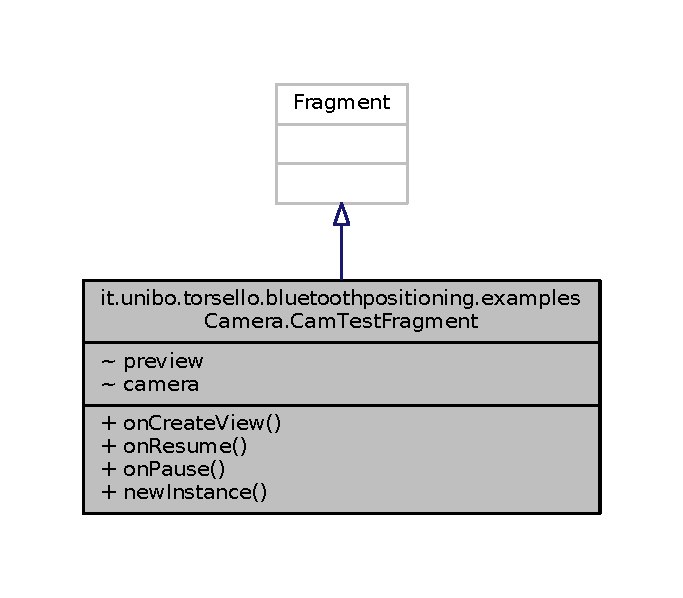
\includegraphics[width=328pt]{classit_1_1unibo_1_1torsello_1_1bluetoothpositioning_1_1examplesCamera_1_1CamTestFragment__inherit__graph}
\end{center}
\end{figure}


Diagramma di collaborazione per it.\+unibo.\+torsello.\+bluetoothpositioning.\+examples\+Camera.\+Cam\+Test\+Fragment\+:
\nopagebreak
\begin{figure}[H]
\begin{center}
\leavevmode
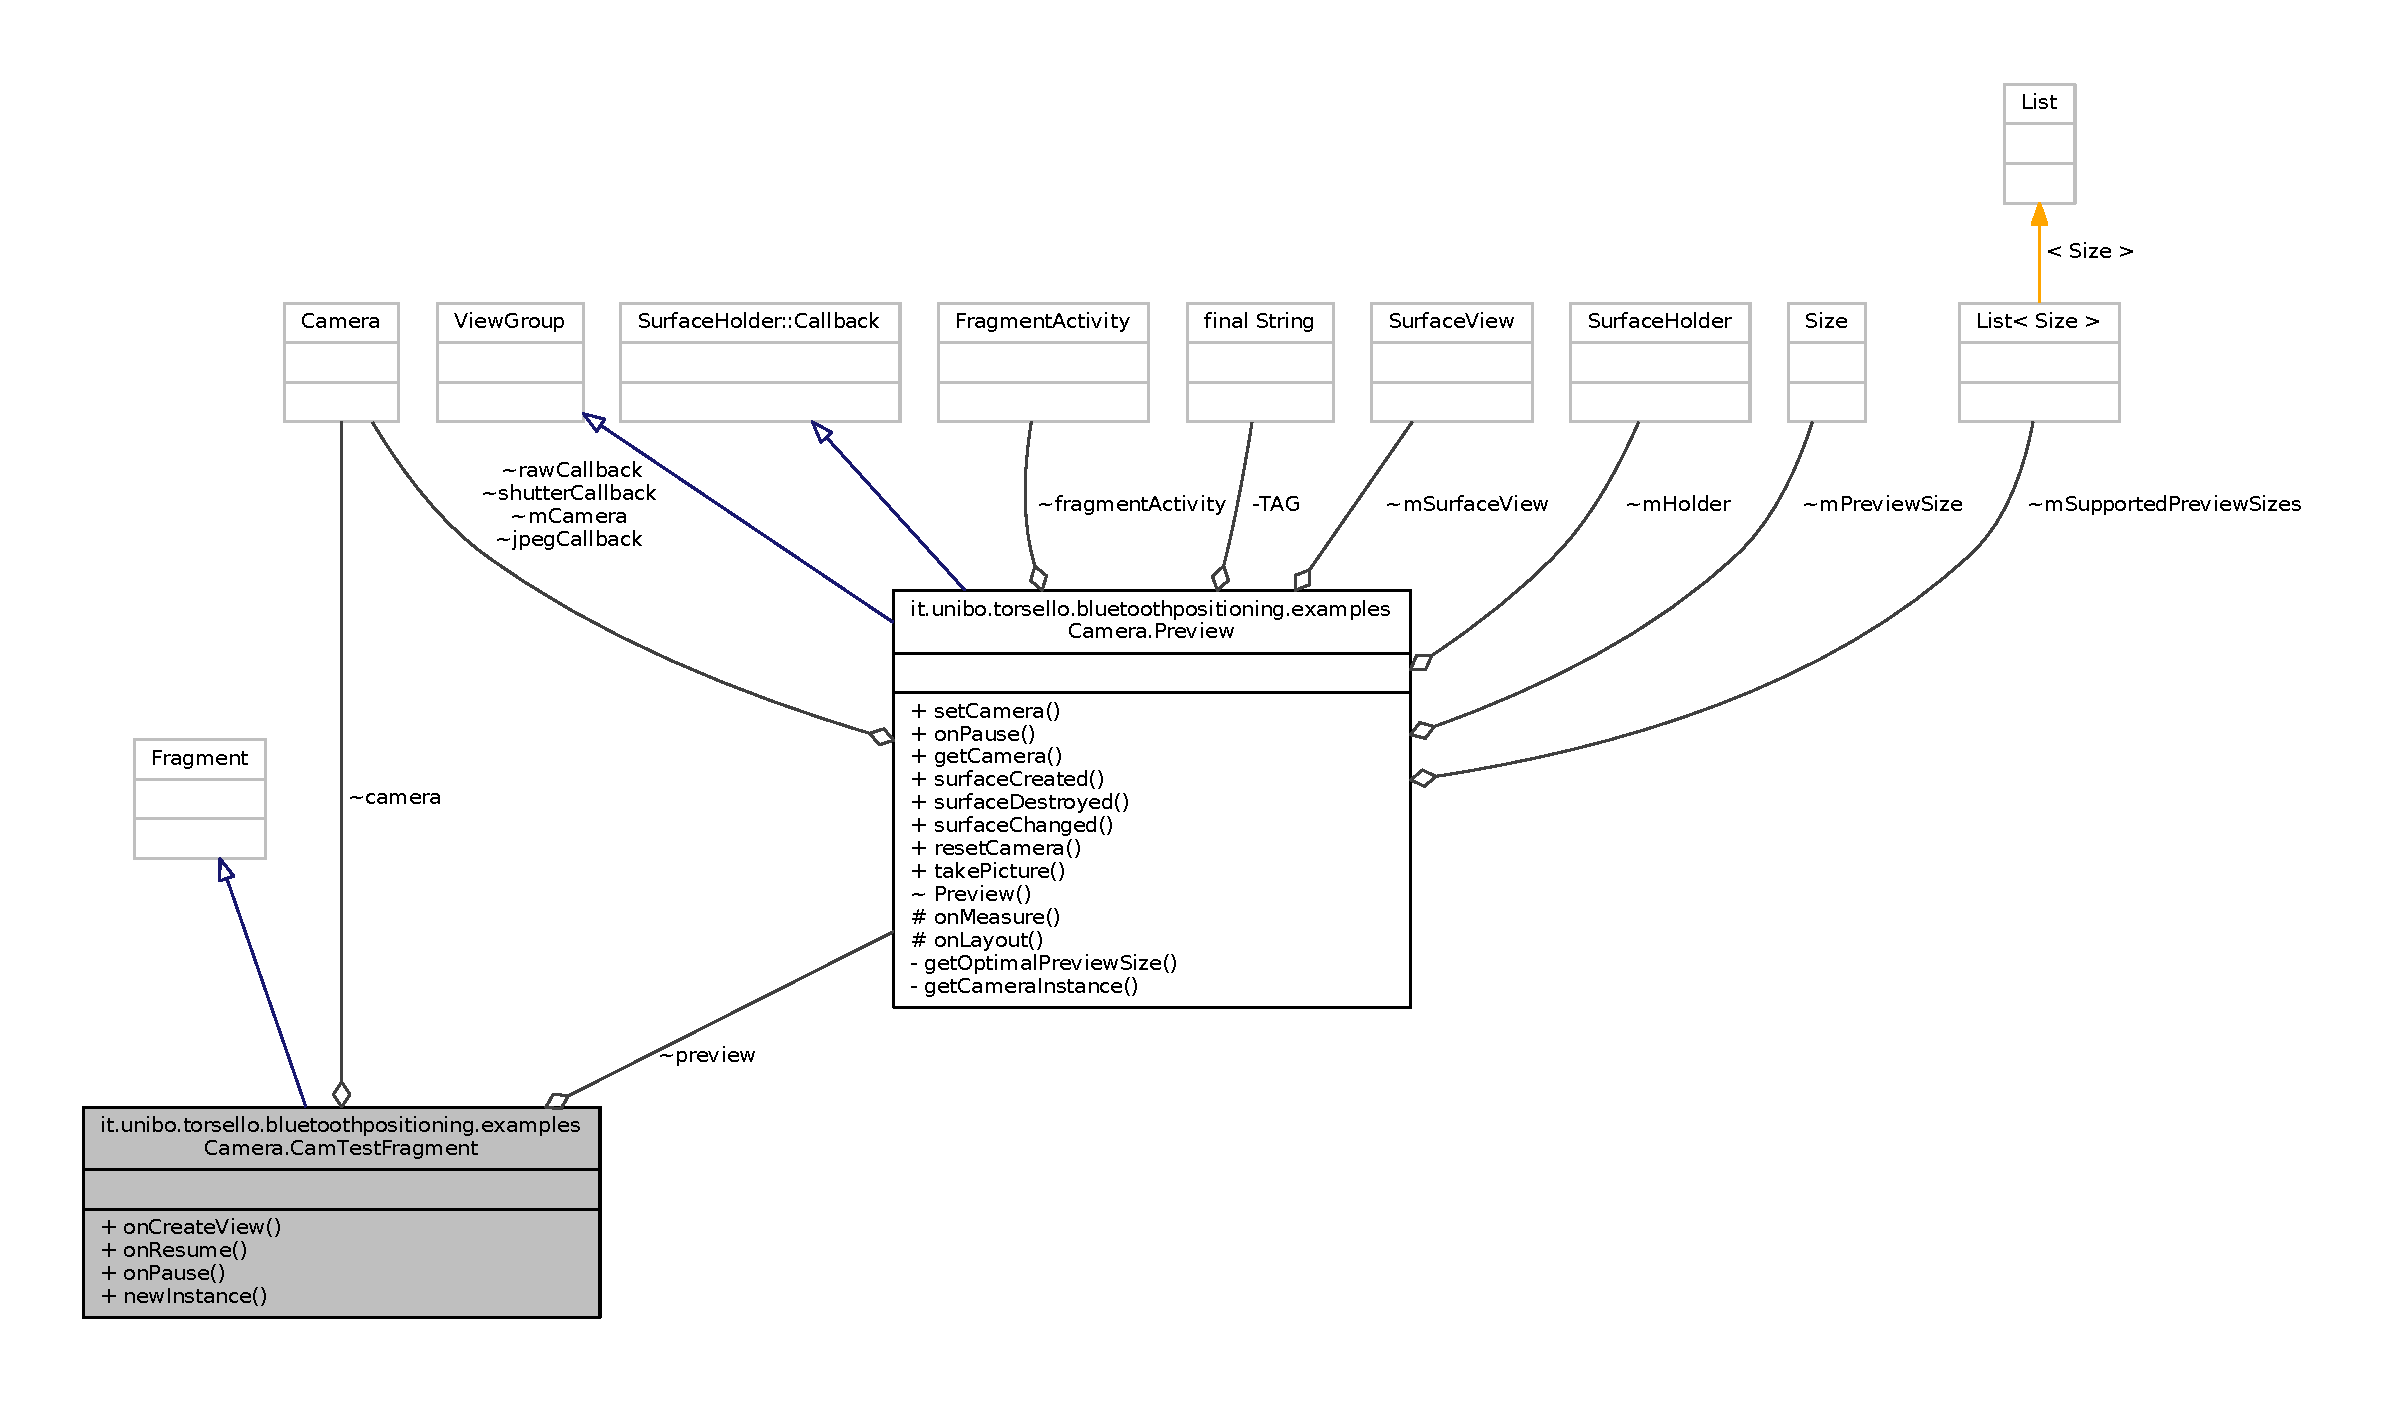
\includegraphics[width=350pt]{classit_1_1unibo_1_1torsello_1_1bluetoothpositioning_1_1examplesCamera_1_1CamTestFragment__coll__graph}
\end{center}
\end{figure}
\subsubsection*{Membri pubblici}
\begin{DoxyCompactItemize}
\item 
View \hyperlink{classit_1_1unibo_1_1torsello_1_1bluetoothpositioning_1_1examplesCamera_1_1CamTestFragment_a197f76a204aaeac1bfb824c41184d12c_a197f76a204aaeac1bfb824c41184d12c}{on\+Create\+View} (Layout\+Inflater inflater, View\+Group container, Bundle saved\+Instance\+State)
\item 
void \hyperlink{classit_1_1unibo_1_1torsello_1_1bluetoothpositioning_1_1examplesCamera_1_1CamTestFragment_a5d9658f3ac7b5ed400a3d4ac6aa62aeb_a5d9658f3ac7b5ed400a3d4ac6aa62aeb}{on\+Resume} ()
\item 
void \hyperlink{classit_1_1unibo_1_1torsello_1_1bluetoothpositioning_1_1examplesCamera_1_1CamTestFragment_ab42acc697b4d94a34ea514a53bc8ce02_ab42acc697b4d94a34ea514a53bc8ce02}{on\+Pause} ()
\end{DoxyCompactItemize}
\subsubsection*{Membri pubblici statici}
\begin{DoxyCompactItemize}
\item 
static \hyperlink{classit_1_1unibo_1_1torsello_1_1bluetoothpositioning_1_1examplesCamera_1_1CamTestFragment}{Cam\+Test\+Fragment} \hyperlink{classit_1_1unibo_1_1torsello_1_1bluetoothpositioning_1_1examplesCamera_1_1CamTestFragment_a90560c7d9a436702707f2e070418e0b7_a90560c7d9a436702707f2e070418e0b7}{new\+Instance} ()
\end{DoxyCompactItemize}
\subsubsection*{Attributi con visibilità di package}
\begin{DoxyCompactItemize}
\item 
\hyperlink{classit_1_1unibo_1_1torsello_1_1bluetoothpositioning_1_1examplesCamera_1_1Preview}{Preview} \hyperlink{classit_1_1unibo_1_1torsello_1_1bluetoothpositioning_1_1examplesCamera_1_1CamTestFragment_ae917d2bc3cab2f7a1641a78cce044fd9_ae917d2bc3cab2f7a1641a78cce044fd9}{preview}
\item 
Camera \hyperlink{classit_1_1unibo_1_1torsello_1_1bluetoothpositioning_1_1examplesCamera_1_1CamTestFragment_ae0d0a876ac5ce037c020f5362d3e1887_ae0d0a876ac5ce037c020f5362d3e1887}{camera}
\end{DoxyCompactItemize}


\subsubsection{Documentazione delle funzioni membro}
\hypertarget{classit_1_1unibo_1_1torsello_1_1bluetoothpositioning_1_1examplesCamera_1_1CamTestFragment_a90560c7d9a436702707f2e070418e0b7_a90560c7d9a436702707f2e070418e0b7}{}\label{classit_1_1unibo_1_1torsello_1_1bluetoothpositioning_1_1examplesCamera_1_1CamTestFragment_a90560c7d9a436702707f2e070418e0b7_a90560c7d9a436702707f2e070418e0b7} 
\index{it\+::unibo\+::torsello\+::bluetoothpositioning\+::examples\+Camera\+::\+Cam\+Test\+Fragment@{it\+::unibo\+::torsello\+::bluetoothpositioning\+::examples\+Camera\+::\+Cam\+Test\+Fragment}!new\+Instance@{new\+Instance}}
\index{new\+Instance@{new\+Instance}!it\+::unibo\+::torsello\+::bluetoothpositioning\+::examples\+Camera\+::\+Cam\+Test\+Fragment@{it\+::unibo\+::torsello\+::bluetoothpositioning\+::examples\+Camera\+::\+Cam\+Test\+Fragment}}
\paragraph{\texorpdfstring{new\+Instance()}{newInstance()}}
{\footnotesize\ttfamily static \hyperlink{classit_1_1unibo_1_1torsello_1_1bluetoothpositioning_1_1examplesCamera_1_1CamTestFragment}{Cam\+Test\+Fragment} it.\+unibo.\+torsello.\+bluetoothpositioning.\+examples\+Camera.\+Cam\+Test\+Fragment.\+new\+Instance (\begin{DoxyParamCaption}{ }\end{DoxyParamCaption})\hspace{0.3cm}{\ttfamily [static]}}


\begin{DoxyCode}
23                                                 \{
24         \textcolor{keywordflow}{return} \textcolor{keyword}{new} CamTestFragment();
25     \}
\end{DoxyCode}
\hypertarget{classit_1_1unibo_1_1torsello_1_1bluetoothpositioning_1_1examplesCamera_1_1CamTestFragment_a197f76a204aaeac1bfb824c41184d12c_a197f76a204aaeac1bfb824c41184d12c}{}\label{classit_1_1unibo_1_1torsello_1_1bluetoothpositioning_1_1examplesCamera_1_1CamTestFragment_a197f76a204aaeac1bfb824c41184d12c_a197f76a204aaeac1bfb824c41184d12c} 
\index{it\+::unibo\+::torsello\+::bluetoothpositioning\+::examples\+Camera\+::\+Cam\+Test\+Fragment@{it\+::unibo\+::torsello\+::bluetoothpositioning\+::examples\+Camera\+::\+Cam\+Test\+Fragment}!on\+Create\+View@{on\+Create\+View}}
\index{on\+Create\+View@{on\+Create\+View}!it\+::unibo\+::torsello\+::bluetoothpositioning\+::examples\+Camera\+::\+Cam\+Test\+Fragment@{it\+::unibo\+::torsello\+::bluetoothpositioning\+::examples\+Camera\+::\+Cam\+Test\+Fragment}}
\paragraph{\texorpdfstring{on\+Create\+View()}{onCreateView()}}
{\footnotesize\ttfamily View it.\+unibo.\+torsello.\+bluetoothpositioning.\+examples\+Camera.\+Cam\+Test\+Fragment.\+on\+Create\+View (\begin{DoxyParamCaption}\item[{Layout\+Inflater}]{inflater,  }\item[{View\+Group}]{container,  }\item[{Bundle}]{saved\+Instance\+State }\end{DoxyParamCaption})}


\begin{DoxyCode}
28                                                                                                       \{
29 
30         View root = inflater.inflate(R.layout.example, container, \textcolor{keyword}{false});
31         \hyperlink{classit_1_1unibo_1_1torsello_1_1bluetoothpositioning_1_1examplesCamera_1_1CamTestFragment_ae917d2bc3cab2f7a1641a78cce044fd9_ae917d2bc3cab2f7a1641a78cce044fd9}{preview} = \textcolor{keyword}{new} Preview(getActivity(), (SurfaceView) root.findViewById(R.id.surfaceView));
32         ((FrameLayout) root.findViewById(R.id.layout)).addView(\hyperlink{classit_1_1unibo_1_1torsello_1_1bluetoothpositioning_1_1examplesCamera_1_1CamTestFragment_ae917d2bc3cab2f7a1641a78cce044fd9_ae917d2bc3cab2f7a1641a78cce044fd9}{preview});
33         \hyperlink{classit_1_1unibo_1_1torsello_1_1bluetoothpositioning_1_1examplesCamera_1_1CamTestFragment_ae917d2bc3cab2f7a1641a78cce044fd9_ae917d2bc3cab2f7a1641a78cce044fd9}{preview}.setKeepScreenOn(\textcolor{keyword}{true});
34         \hyperlink{classit_1_1unibo_1_1torsello_1_1bluetoothpositioning_1_1examplesCamera_1_1CamTestFragment_ae917d2bc3cab2f7a1641a78cce044fd9_ae917d2bc3cab2f7a1641a78cce044fd9}{preview}.setOnClickListener(\textcolor{keyword}{new} OnClickListener() \{
35 
36             @Override
37             \textcolor{keyword}{public} \textcolor{keywordtype}{void} onClick(View arg0) \{
38                 \hyperlink{classit_1_1unibo_1_1torsello_1_1bluetoothpositioning_1_1examplesCamera_1_1CamTestFragment_ae917d2bc3cab2f7a1641a78cce044fd9_ae917d2bc3cab2f7a1641a78cce044fd9}{preview}.\hyperlink{classit_1_1unibo_1_1torsello_1_1bluetoothpositioning_1_1examplesCamera_1_1Preview_afa7f533cc47be1bf7be2b1d1bfa43600_afa7f533cc47be1bf7be2b1d1bfa43600}{takePicture}();
39             \}
40         \});
41         \hyperlink{classit_1_1unibo_1_1torsello_1_1bluetoothpositioning_1_1examplesCamera_1_1CamTestFragment_ae917d2bc3cab2f7a1641a78cce044fd9_ae917d2bc3cab2f7a1641a78cce044fd9}{preview}.setOnLongClickListener(\textcolor{keyword}{new} View.OnLongClickListener() \{
42             @Override
43             \textcolor{keyword}{public} \textcolor{keywordtype}{boolean} onLongClick(View arg0) \{
44 
45                 \hyperlink{classit_1_1unibo_1_1torsello_1_1bluetoothpositioning_1_1examplesCamera_1_1CamTestFragment_ae0d0a876ac5ce037c020f5362d3e1887_ae0d0a876ac5ce037c020f5362d3e1887}{camera}.autoFocus(\textcolor{keyword}{new} Camera.AutoFocusCallback() \{
46                     @Override
47                     \textcolor{keyword}{public} \textcolor{keywordtype}{void} onAutoFocus(\textcolor{keywordtype}{boolean} success, Camera arg1) \{
48                         \textcolor{keywordflow}{if} (success) \{
49                             \hyperlink{classit_1_1unibo_1_1torsello_1_1bluetoothpositioning_1_1examplesCamera_1_1CamTestFragment_ae917d2bc3cab2f7a1641a78cce044fd9_ae917d2bc3cab2f7a1641a78cce044fd9}{preview}.\hyperlink{classit_1_1unibo_1_1torsello_1_1bluetoothpositioning_1_1examplesCamera_1_1Preview_afa7f533cc47be1bf7be2b1d1bfa43600_afa7f533cc47be1bf7be2b1d1bfa43600}{takePicture}();
50                         \}
51                     \}
52                 \});
53                 \textcolor{keywordflow}{return} \textcolor{keyword}{true};
54             \}
55         \});
56         \textcolor{keywordflow}{return} root;
57     \}
\end{DoxyCode}
\hypertarget{classit_1_1unibo_1_1torsello_1_1bluetoothpositioning_1_1examplesCamera_1_1CamTestFragment_ab42acc697b4d94a34ea514a53bc8ce02_ab42acc697b4d94a34ea514a53bc8ce02}{}\label{classit_1_1unibo_1_1torsello_1_1bluetoothpositioning_1_1examplesCamera_1_1CamTestFragment_ab42acc697b4d94a34ea514a53bc8ce02_ab42acc697b4d94a34ea514a53bc8ce02} 
\index{it\+::unibo\+::torsello\+::bluetoothpositioning\+::examples\+Camera\+::\+Cam\+Test\+Fragment@{it\+::unibo\+::torsello\+::bluetoothpositioning\+::examples\+Camera\+::\+Cam\+Test\+Fragment}!on\+Pause@{on\+Pause}}
\index{on\+Pause@{on\+Pause}!it\+::unibo\+::torsello\+::bluetoothpositioning\+::examples\+Camera\+::\+Cam\+Test\+Fragment@{it\+::unibo\+::torsello\+::bluetoothpositioning\+::examples\+Camera\+::\+Cam\+Test\+Fragment}}
\paragraph{\texorpdfstring{on\+Pause()}{onPause()}}
{\footnotesize\ttfamily void it.\+unibo.\+torsello.\+bluetoothpositioning.\+examples\+Camera.\+Cam\+Test\+Fragment.\+on\+Pause (\begin{DoxyParamCaption}{ }\end{DoxyParamCaption})}


\begin{DoxyCode}
67                           \{
68         \hyperlink{classit_1_1unibo_1_1torsello_1_1bluetoothpositioning_1_1examplesCamera_1_1CamTestFragment_ae917d2bc3cab2f7a1641a78cce044fd9_ae917d2bc3cab2f7a1641a78cce044fd9}{preview}.\hyperlink{classit_1_1unibo_1_1torsello_1_1bluetoothpositioning_1_1examplesCamera_1_1Preview_af63fabacd267ab2763cc3183464dbf47_af63fabacd267ab2763cc3183464dbf47}{onPause}();
69         super.onPause();
70     \}
\end{DoxyCode}
\hypertarget{classit_1_1unibo_1_1torsello_1_1bluetoothpositioning_1_1examplesCamera_1_1CamTestFragment_a5d9658f3ac7b5ed400a3d4ac6aa62aeb_a5d9658f3ac7b5ed400a3d4ac6aa62aeb}{}\label{classit_1_1unibo_1_1torsello_1_1bluetoothpositioning_1_1examplesCamera_1_1CamTestFragment_a5d9658f3ac7b5ed400a3d4ac6aa62aeb_a5d9658f3ac7b5ed400a3d4ac6aa62aeb} 
\index{it\+::unibo\+::torsello\+::bluetoothpositioning\+::examples\+Camera\+::\+Cam\+Test\+Fragment@{it\+::unibo\+::torsello\+::bluetoothpositioning\+::examples\+Camera\+::\+Cam\+Test\+Fragment}!on\+Resume@{on\+Resume}}
\index{on\+Resume@{on\+Resume}!it\+::unibo\+::torsello\+::bluetoothpositioning\+::examples\+Camera\+::\+Cam\+Test\+Fragment@{it\+::unibo\+::torsello\+::bluetoothpositioning\+::examples\+Camera\+::\+Cam\+Test\+Fragment}}
\paragraph{\texorpdfstring{on\+Resume()}{onResume()}}
{\footnotesize\ttfamily void it.\+unibo.\+torsello.\+bluetoothpositioning.\+examples\+Camera.\+Cam\+Test\+Fragment.\+on\+Resume (\begin{DoxyParamCaption}{ }\end{DoxyParamCaption})}


\begin{DoxyCode}
60                            \{
61         super.onResume();
62         \hyperlink{classit_1_1unibo_1_1torsello_1_1bluetoothpositioning_1_1examplesCamera_1_1CamTestFragment_ae917d2bc3cab2f7a1641a78cce044fd9_ae917d2bc3cab2f7a1641a78cce044fd9}{preview}.\hyperlink{classit_1_1unibo_1_1torsello_1_1bluetoothpositioning_1_1examplesCamera_1_1Preview_a018960081707cd70025fb4b7e0322162_a018960081707cd70025fb4b7e0322162}{setCamera}(getActivity());
63         \hyperlink{classit_1_1unibo_1_1torsello_1_1bluetoothpositioning_1_1examplesCamera_1_1CamTestFragment_ae0d0a876ac5ce037c020f5362d3e1887_ae0d0a876ac5ce037c020f5362d3e1887}{camera} = \hyperlink{classit_1_1unibo_1_1torsello_1_1bluetoothpositioning_1_1examplesCamera_1_1CamTestFragment_ae917d2bc3cab2f7a1641a78cce044fd9_ae917d2bc3cab2f7a1641a78cce044fd9}{preview}.\hyperlink{classit_1_1unibo_1_1torsello_1_1bluetoothpositioning_1_1examplesCamera_1_1Preview_a8bc995f4776255800f64dfb94d38e47d_a8bc995f4776255800f64dfb94d38e47d}{getCamera}();
64     \}
\end{DoxyCode}


\subsubsection{Documentazione dei membri dato}
\hypertarget{classit_1_1unibo_1_1torsello_1_1bluetoothpositioning_1_1examplesCamera_1_1CamTestFragment_ae0d0a876ac5ce037c020f5362d3e1887_ae0d0a876ac5ce037c020f5362d3e1887}{}\label{classit_1_1unibo_1_1torsello_1_1bluetoothpositioning_1_1examplesCamera_1_1CamTestFragment_ae0d0a876ac5ce037c020f5362d3e1887_ae0d0a876ac5ce037c020f5362d3e1887} 
\index{it\+::unibo\+::torsello\+::bluetoothpositioning\+::examples\+Camera\+::\+Cam\+Test\+Fragment@{it\+::unibo\+::torsello\+::bluetoothpositioning\+::examples\+Camera\+::\+Cam\+Test\+Fragment}!camera@{camera}}
\index{camera@{camera}!it\+::unibo\+::torsello\+::bluetoothpositioning\+::examples\+Camera\+::\+Cam\+Test\+Fragment@{it\+::unibo\+::torsello\+::bluetoothpositioning\+::examples\+Camera\+::\+Cam\+Test\+Fragment}}
\paragraph{\texorpdfstring{camera}{camera}}
{\footnotesize\ttfamily Camera it.\+unibo.\+torsello.\+bluetoothpositioning.\+examples\+Camera.\+Cam\+Test\+Fragment.\+camera\hspace{0.3cm}{\ttfamily [package]}}

\hypertarget{classit_1_1unibo_1_1torsello_1_1bluetoothpositioning_1_1examplesCamera_1_1CamTestFragment_ae917d2bc3cab2f7a1641a78cce044fd9_ae917d2bc3cab2f7a1641a78cce044fd9}{}\label{classit_1_1unibo_1_1torsello_1_1bluetoothpositioning_1_1examplesCamera_1_1CamTestFragment_ae917d2bc3cab2f7a1641a78cce044fd9_ae917d2bc3cab2f7a1641a78cce044fd9} 
\index{it\+::unibo\+::torsello\+::bluetoothpositioning\+::examples\+Camera\+::\+Cam\+Test\+Fragment@{it\+::unibo\+::torsello\+::bluetoothpositioning\+::examples\+Camera\+::\+Cam\+Test\+Fragment}!preview@{preview}}
\index{preview@{preview}!it\+::unibo\+::torsello\+::bluetoothpositioning\+::examples\+Camera\+::\+Cam\+Test\+Fragment@{it\+::unibo\+::torsello\+::bluetoothpositioning\+::examples\+Camera\+::\+Cam\+Test\+Fragment}}
\paragraph{\texorpdfstring{preview}{preview}}
{\footnotesize\ttfamily \hyperlink{classit_1_1unibo_1_1torsello_1_1bluetoothpositioning_1_1examplesCamera_1_1Preview}{Preview} it.\+unibo.\+torsello.\+bluetoothpositioning.\+examples\+Camera.\+Cam\+Test\+Fragment.\+preview\hspace{0.3cm}{\ttfamily [package]}}



La documentazione per questa classe è stata generata a partire dal seguente file\+:\begin{DoxyCompactItemize}
\item 
\hyperlink{CamTestFragment_8java}{Cam\+Test\+Fragment.\+java}\end{DoxyCompactItemize}

\hypertarget{classit_1_1unibo_1_1torsello_1_1bluetoothpositioning_1_1util_1_1ChartUtil}{}\subsection{Riferimenti per la classe it.\+unibo.\+torsello.\+bluetoothpositioning.\+util.\+Chart\+Util}
\label{classit_1_1unibo_1_1torsello_1_1bluetoothpositioning_1_1util_1_1ChartUtil}\index{it.\+unibo.\+torsello.\+bluetoothpositioning.\+util.\+Chart\+Util@{it.\+unibo.\+torsello.\+bluetoothpositioning.\+util.\+Chart\+Util}}


Diagramma delle classi per it.\+unibo.\+torsello.\+bluetoothpositioning.\+util.\+Chart\+Util
\nopagebreak
\begin{figure}[H]
\begin{center}
\leavevmode
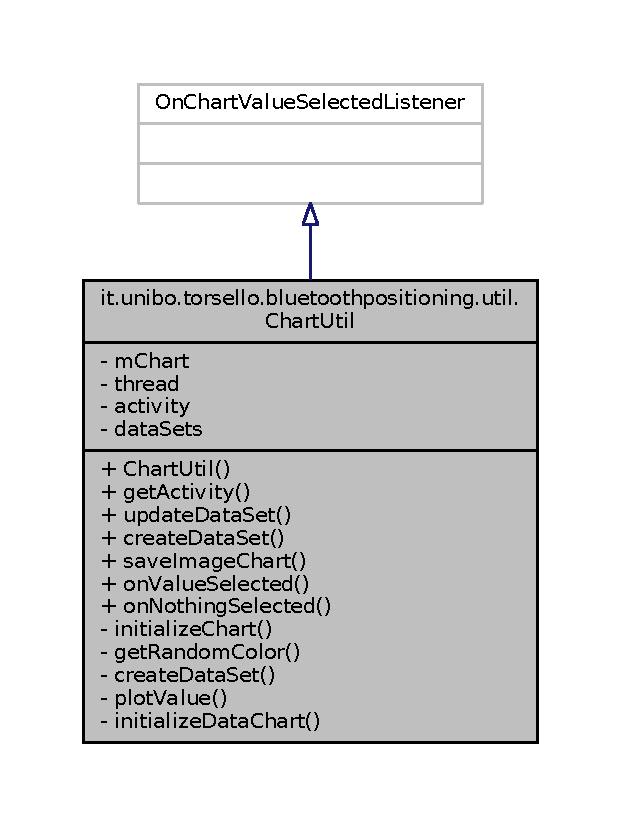
\includegraphics[width=298pt]{classit_1_1unibo_1_1torsello_1_1bluetoothpositioning_1_1util_1_1ChartUtil__inherit__graph}
\end{center}
\end{figure}


Diagramma di collaborazione per it.\+unibo.\+torsello.\+bluetoothpositioning.\+util.\+Chart\+Util\+:
\nopagebreak
\begin{figure}[H]
\begin{center}
\leavevmode
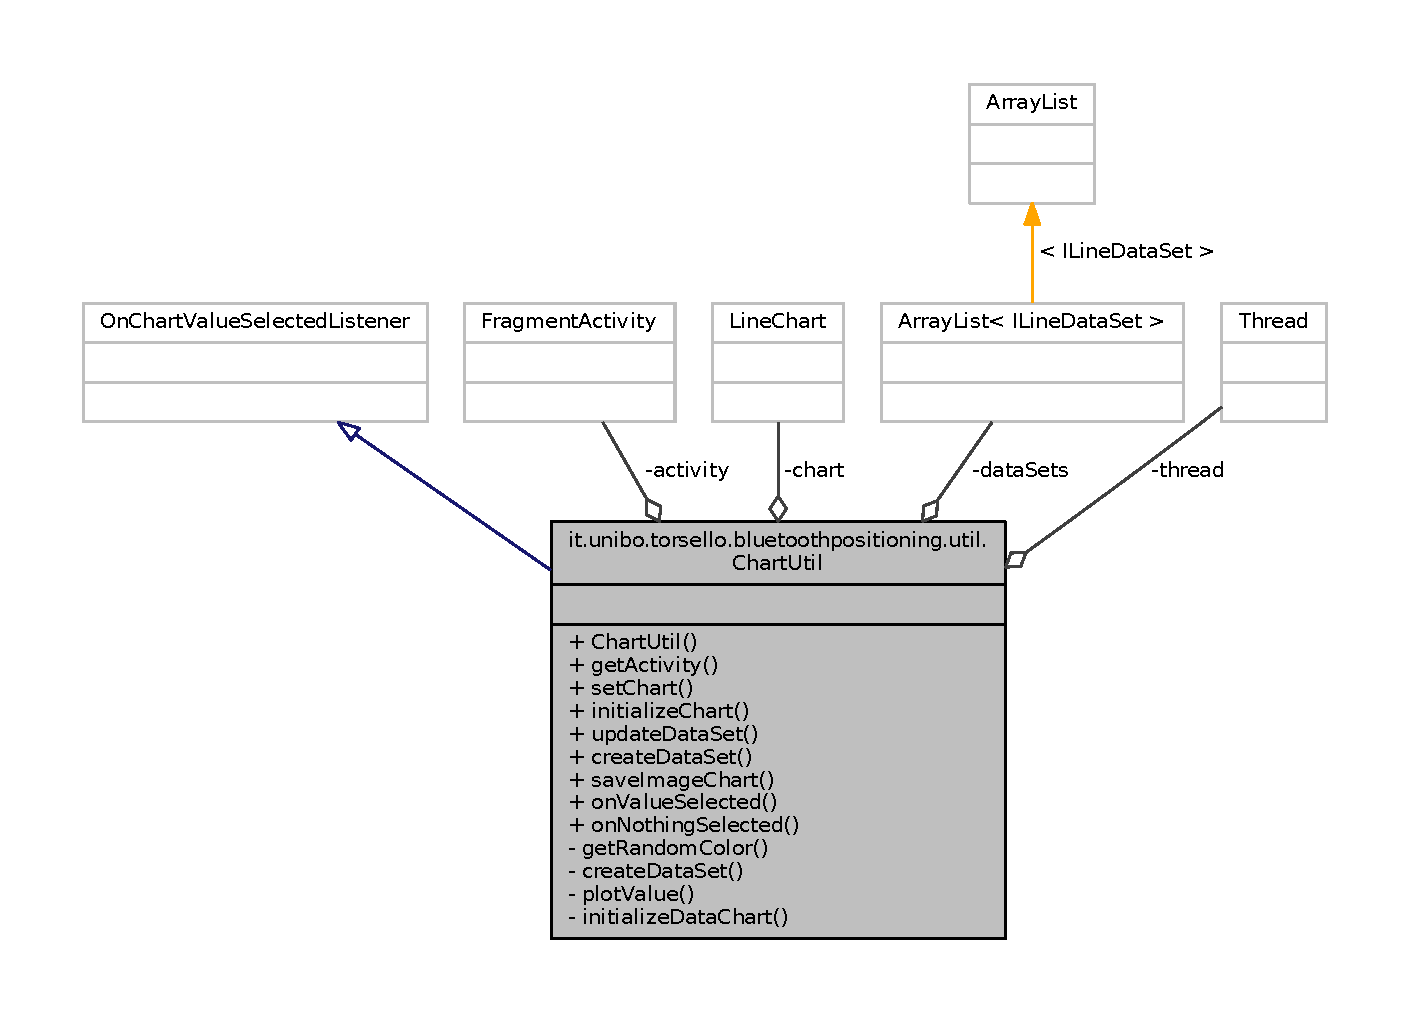
\includegraphics[width=350pt]{classit_1_1unibo_1_1torsello_1_1bluetoothpositioning_1_1util_1_1ChartUtil__coll__graph}
\end{center}
\end{figure}
\subsubsection*{Membri pubblici}
\begin{DoxyCompactItemize}
\item 
\hyperlink{classit_1_1unibo_1_1torsello_1_1bluetoothpositioning_1_1util_1_1ChartUtil_a255b439c7574dc7858355e3fc71ca6f7_a255b439c7574dc7858355e3fc71ca6f7}{Chart\+Util} (Fragment\+Activity fragment\+Activity)
\item 
Fragment\+Activity \hyperlink{classit_1_1unibo_1_1torsello_1_1bluetoothpositioning_1_1util_1_1ChartUtil_a59150a6d20b6d0ad2fcf8c1ba858d355_a59150a6d20b6d0ad2fcf8c1ba858d355}{get\+Activity} ()
\item 
void \hyperlink{classit_1_1unibo_1_1torsello_1_1bluetoothpositioning_1_1util_1_1ChartUtil_a26e84414723ff1ca38d8f2907ed3322e_a26e84414723ff1ca38d8f2907ed3322e}{set\+Chart} (Line\+Chart \hyperlink{classit_1_1unibo_1_1torsello_1_1bluetoothpositioning_1_1util_1_1ChartUtil_a6c34176fdfb85bac1d3aa1529b49ad5f_a6c34176fdfb85bac1d3aa1529b49ad5f}{chart})
\item 
void \hyperlink{classit_1_1unibo_1_1torsello_1_1bluetoothpositioning_1_1util_1_1ChartUtil_aab1a6bd41cbf8228c53d633af6b89bb7_aab1a6bd41cbf8228c53d633af6b89bb7}{initialize\+Chart} ()
\item 
void \hyperlink{classit_1_1unibo_1_1torsello_1_1bluetoothpositioning_1_1util_1_1ChartUtil_aa9bda04d2c2058fb1b3fcd72c5a7471d_aa9bda04d2c2058fb1b3fcd72c5a7471d}{update\+Data\+Set} (final Array\+List$<$ Double $>$ double\+Array\+List)
\item 
void \hyperlink{classit_1_1unibo_1_1torsello_1_1bluetoothpositioning_1_1util_1_1ChartUtil_a7460cb57f8ad402dc522b592bc40f7b2_a7460cb57f8ad402dc522b592bc40f7b2}{create\+Data\+Set} (Array\+List$<$ String $>$ args)
\item 
void \hyperlink{classit_1_1unibo_1_1torsello_1_1bluetoothpositioning_1_1util_1_1ChartUtil_afdbdcf15b073da5b03613dbccc7681a9_afdbdcf15b073da5b03613dbccc7681a9}{save\+Image\+Chart} (String chart\+Name, String formatted\+Date)
\item 
void \hyperlink{classit_1_1unibo_1_1torsello_1_1bluetoothpositioning_1_1util_1_1ChartUtil_a7f7609b8236d269e4f272f717b0b0294_a7f7609b8236d269e4f272f717b0b0294}{on\+Value\+Selected} (Entry e, Highlight h)
\item 
void \hyperlink{classit_1_1unibo_1_1torsello_1_1bluetoothpositioning_1_1util_1_1ChartUtil_a7e7f15aebf87926e19bc9e1ece289fde_a7e7f15aebf87926e19bc9e1ece289fde}{on\+Nothing\+Selected} ()
\end{DoxyCompactItemize}
\subsubsection*{Membri privati}
\begin{DoxyCompactItemize}
\item 
int \hyperlink{classit_1_1unibo_1_1torsello_1_1bluetoothpositioning_1_1util_1_1ChartUtil_ac7dc0a849201a4a3c932fd525435b397_ac7dc0a849201a4a3c932fd525435b397}{get\+Random\+Color} ()
\item 
Line\+Data\+Set \hyperlink{classit_1_1unibo_1_1torsello_1_1bluetoothpositioning_1_1util_1_1ChartUtil_a7e24ac167fd4955090e04024b11c6c31_a7e24ac167fd4955090e04024b11c6c31}{create\+Data\+Set} (String name\+Data\+Set, int color)
\item 
void \hyperlink{classit_1_1unibo_1_1torsello_1_1bluetoothpositioning_1_1util_1_1ChartUtil_a86398d4aca978fbfc10c71039191635e_a86398d4aca978fbfc10c71039191635e}{plot\+Value} (Line\+Data data, int index, Double value)
\item 
void \hyperlink{classit_1_1unibo_1_1torsello_1_1bluetoothpositioning_1_1util_1_1ChartUtil_a3393d9aa353849188c02a63d64f2dd2d_a3393d9aa353849188c02a63d64f2dd2d}{initialize\+Data\+Chart} (Array\+List$<$ I\+Line\+Data\+Set $>$ \hyperlink{classit_1_1unibo_1_1torsello_1_1bluetoothpositioning_1_1util_1_1ChartUtil_aa98bcaa2d5ba444b91cdc029768d380a_aa98bcaa2d5ba444b91cdc029768d380a}{data\+Sets})
\end{DoxyCompactItemize}
\subsubsection*{Attributi privati}
\begin{DoxyCompactItemize}
\item 
Line\+Chart \hyperlink{classit_1_1unibo_1_1torsello_1_1bluetoothpositioning_1_1util_1_1ChartUtil_a6c34176fdfb85bac1d3aa1529b49ad5f_a6c34176fdfb85bac1d3aa1529b49ad5f}{chart}
\item 
Thread \hyperlink{classit_1_1unibo_1_1torsello_1_1bluetoothpositioning_1_1util_1_1ChartUtil_ac73af861c9ca49e226fe1218cef6c572_ac73af861c9ca49e226fe1218cef6c572}{thread}
\item 
Fragment\+Activity \hyperlink{classit_1_1unibo_1_1torsello_1_1bluetoothpositioning_1_1util_1_1ChartUtil_acf9c1988f7aaacc3f3354ac7e9eeef6a_acf9c1988f7aaacc3f3354ac7e9eeef6a}{activity}
\item 
Array\+List$<$ I\+Line\+Data\+Set $>$ \hyperlink{classit_1_1unibo_1_1torsello_1_1bluetoothpositioning_1_1util_1_1ChartUtil_aa98bcaa2d5ba444b91cdc029768d380a_aa98bcaa2d5ba444b91cdc029768d380a}{data\+Sets}
\end{DoxyCompactItemize}


\subsubsection{Descrizione dettagliata}
Created by Federico Torsello. \href{mailto:federico.torsello@studio.unibo.it}{\tt federico.\+torsello@studio.\+unibo.\+it} 

\subsubsection{Documentazione dei costruttori e dei distruttori}
\hypertarget{classit_1_1unibo_1_1torsello_1_1bluetoothpositioning_1_1util_1_1ChartUtil_a255b439c7574dc7858355e3fc71ca6f7_a255b439c7574dc7858355e3fc71ca6f7}{}\label{classit_1_1unibo_1_1torsello_1_1bluetoothpositioning_1_1util_1_1ChartUtil_a255b439c7574dc7858355e3fc71ca6f7_a255b439c7574dc7858355e3fc71ca6f7} 
\index{it\+::unibo\+::torsello\+::bluetoothpositioning\+::util\+::\+Chart\+Util@{it\+::unibo\+::torsello\+::bluetoothpositioning\+::util\+::\+Chart\+Util}!Chart\+Util@{Chart\+Util}}
\index{Chart\+Util@{Chart\+Util}!it\+::unibo\+::torsello\+::bluetoothpositioning\+::util\+::\+Chart\+Util@{it\+::unibo\+::torsello\+::bluetoothpositioning\+::util\+::\+Chart\+Util}}
\paragraph{\texorpdfstring{Chart\+Util()}{ChartUtil()}}
{\footnotesize\ttfamily it.\+unibo.\+torsello.\+bluetoothpositioning.\+util.\+Chart\+Util.\+Chart\+Util (\begin{DoxyParamCaption}\item[{Fragment\+Activity}]{fragment\+Activity }\end{DoxyParamCaption})}


\begin{DoxyCode}
42                                                         \{
43         this.\hyperlink{classit_1_1unibo_1_1torsello_1_1bluetoothpositioning_1_1util_1_1ChartUtil_acf9c1988f7aaacc3f3354ac7e9eeef6a_acf9c1988f7aaacc3f3354ac7e9eeef6a}{activity} = fragmentActivity;
44     \}
\end{DoxyCode}


\subsubsection{Documentazione delle funzioni membro}
\hypertarget{classit_1_1unibo_1_1torsello_1_1bluetoothpositioning_1_1util_1_1ChartUtil_a7460cb57f8ad402dc522b592bc40f7b2_a7460cb57f8ad402dc522b592bc40f7b2}{}\label{classit_1_1unibo_1_1torsello_1_1bluetoothpositioning_1_1util_1_1ChartUtil_a7460cb57f8ad402dc522b592bc40f7b2_a7460cb57f8ad402dc522b592bc40f7b2} 
\index{it\+::unibo\+::torsello\+::bluetoothpositioning\+::util\+::\+Chart\+Util@{it\+::unibo\+::torsello\+::bluetoothpositioning\+::util\+::\+Chart\+Util}!create\+Data\+Set@{create\+Data\+Set}}
\index{create\+Data\+Set@{create\+Data\+Set}!it\+::unibo\+::torsello\+::bluetoothpositioning\+::util\+::\+Chart\+Util@{it\+::unibo\+::torsello\+::bluetoothpositioning\+::util\+::\+Chart\+Util}}
\paragraph{\texorpdfstring{create\+Data\+Set()}{createDataSet()}\hspace{0.1cm}{\footnotesize\ttfamily [1/2]}}
{\footnotesize\ttfamily void it.\+unibo.\+torsello.\+bluetoothpositioning.\+util.\+Chart\+Util.\+create\+Data\+Set (\begin{DoxyParamCaption}\item[{Array\+List$<$ String $>$}]{args }\end{DoxyParamCaption})}


\begin{DoxyCode}
133                                                       \{
134         \textcolor{comment}{// create a dataset and give it a type}
135 
136         \textcolor{keywordflow}{for} (String s : args) \{
137             \textcolor{keywordflow}{if} (s != null) \{
138                 \textcolor{keywordflow}{if} (s.equals(\hyperlink{classit_1_1unibo_1_1torsello_1_1bluetoothpositioning_1_1util_1_1ChartUtil_a59150a6d20b6d0ad2fcf8c1ba858d355_a59150a6d20b6d0ad2fcf8c1ba858d355}{getActivity}().getString(R.string.chart\_arduino))) \{
139                     \hyperlink{classit_1_1unibo_1_1torsello_1_1bluetoothpositioning_1_1util_1_1ChartUtil_aa98bcaa2d5ba444b91cdc029768d380a_aa98bcaa2d5ba444b91cdc029768d380a}{dataSets}.add(\hyperlink{classit_1_1unibo_1_1torsello_1_1bluetoothpositioning_1_1util_1_1ChartUtil_a7460cb57f8ad402dc522b592bc40f7b2_a7460cb57f8ad402dc522b592bc40f7b2}{createDataSet}(s, Color.RED));
140                 \} \textcolor{keywordflow}{else} \{
141                     \hyperlink{classit_1_1unibo_1_1torsello_1_1bluetoothpositioning_1_1util_1_1ChartUtil_aa98bcaa2d5ba444b91cdc029768d380a_aa98bcaa2d5ba444b91cdc029768d380a}{dataSets}.add(\hyperlink{classit_1_1unibo_1_1torsello_1_1bluetoothpositioning_1_1util_1_1ChartUtil_a7460cb57f8ad402dc522b592bc40f7b2_a7460cb57f8ad402dc522b592bc40f7b2}{createDataSet}(s, 
      \hyperlink{classit_1_1unibo_1_1torsello_1_1bluetoothpositioning_1_1util_1_1ChartUtil_ac7dc0a849201a4a3c932fd525435b397_ac7dc0a849201a4a3c932fd525435b397}{getRandomColor}()));
142                 \}
143             \}
144         \}
145 
146     \}
\end{DoxyCode}
\hypertarget{classit_1_1unibo_1_1torsello_1_1bluetoothpositioning_1_1util_1_1ChartUtil_a7e24ac167fd4955090e04024b11c6c31_a7e24ac167fd4955090e04024b11c6c31}{}\label{classit_1_1unibo_1_1torsello_1_1bluetoothpositioning_1_1util_1_1ChartUtil_a7e24ac167fd4955090e04024b11c6c31_a7e24ac167fd4955090e04024b11c6c31} 
\index{it\+::unibo\+::torsello\+::bluetoothpositioning\+::util\+::\+Chart\+Util@{it\+::unibo\+::torsello\+::bluetoothpositioning\+::util\+::\+Chart\+Util}!create\+Data\+Set@{create\+Data\+Set}}
\index{create\+Data\+Set@{create\+Data\+Set}!it\+::unibo\+::torsello\+::bluetoothpositioning\+::util\+::\+Chart\+Util@{it\+::unibo\+::torsello\+::bluetoothpositioning\+::util\+::\+Chart\+Util}}
\paragraph{\texorpdfstring{create\+Data\+Set()}{createDataSet()}\hspace{0.1cm}{\footnotesize\ttfamily [2/2]}}
{\footnotesize\ttfamily Line\+Data\+Set it.\+unibo.\+torsello.\+bluetoothpositioning.\+util.\+Chart\+Util.\+create\+Data\+Set (\begin{DoxyParamCaption}\item[{String}]{name\+Data\+Set,  }\item[{int}]{color }\end{DoxyParamCaption})\hspace{0.3cm}{\ttfamily [private]}}


\begin{DoxyCode}
157                                                                      \{
158         LineDataSet \textcolor{keyword}{set} = \textcolor{keyword}{new} LineDataSet(null, nameDataSet);
159         \textcolor{keyword}{set}.setColor(color);
160         \textcolor{keywordflow}{return} \textcolor{keyword}{set};
161     \}
\end{DoxyCode}
\hypertarget{classit_1_1unibo_1_1torsello_1_1bluetoothpositioning_1_1util_1_1ChartUtil_a59150a6d20b6d0ad2fcf8c1ba858d355_a59150a6d20b6d0ad2fcf8c1ba858d355}{}\label{classit_1_1unibo_1_1torsello_1_1bluetoothpositioning_1_1util_1_1ChartUtil_a59150a6d20b6d0ad2fcf8c1ba858d355_a59150a6d20b6d0ad2fcf8c1ba858d355} 
\index{it\+::unibo\+::torsello\+::bluetoothpositioning\+::util\+::\+Chart\+Util@{it\+::unibo\+::torsello\+::bluetoothpositioning\+::util\+::\+Chart\+Util}!get\+Activity@{get\+Activity}}
\index{get\+Activity@{get\+Activity}!it\+::unibo\+::torsello\+::bluetoothpositioning\+::util\+::\+Chart\+Util@{it\+::unibo\+::torsello\+::bluetoothpositioning\+::util\+::\+Chart\+Util}}
\paragraph{\texorpdfstring{get\+Activity()}{getActivity()}}
{\footnotesize\ttfamily Fragment\+Activity it.\+unibo.\+torsello.\+bluetoothpositioning.\+util.\+Chart\+Util.\+get\+Activity (\begin{DoxyParamCaption}{ }\end{DoxyParamCaption})}


\begin{DoxyCode}
46                                           \{
47         \textcolor{keywordflow}{return} \hyperlink{classit_1_1unibo_1_1torsello_1_1bluetoothpositioning_1_1util_1_1ChartUtil_acf9c1988f7aaacc3f3354ac7e9eeef6a_acf9c1988f7aaacc3f3354ac7e9eeef6a}{activity};
48     \}
\end{DoxyCode}
\hypertarget{classit_1_1unibo_1_1torsello_1_1bluetoothpositioning_1_1util_1_1ChartUtil_ac7dc0a849201a4a3c932fd525435b397_ac7dc0a849201a4a3c932fd525435b397}{}\label{classit_1_1unibo_1_1torsello_1_1bluetoothpositioning_1_1util_1_1ChartUtil_ac7dc0a849201a4a3c932fd525435b397_ac7dc0a849201a4a3c932fd525435b397} 
\index{it\+::unibo\+::torsello\+::bluetoothpositioning\+::util\+::\+Chart\+Util@{it\+::unibo\+::torsello\+::bluetoothpositioning\+::util\+::\+Chart\+Util}!get\+Random\+Color@{get\+Random\+Color}}
\index{get\+Random\+Color@{get\+Random\+Color}!it\+::unibo\+::torsello\+::bluetoothpositioning\+::util\+::\+Chart\+Util@{it\+::unibo\+::torsello\+::bluetoothpositioning\+::util\+::\+Chart\+Util}}
\paragraph{\texorpdfstring{get\+Random\+Color()}{getRandomColor()}}
{\footnotesize\ttfamily int it.\+unibo.\+torsello.\+bluetoothpositioning.\+util.\+Chart\+Util.\+get\+Random\+Color (\begin{DoxyParamCaption}{ }\end{DoxyParamCaption})\hspace{0.3cm}{\ttfamily [private]}}


\begin{DoxyCode}
148                                  \{
149         Random rnd = \textcolor{keyword}{new} Random();
150         \textcolor{keywordtype}{int} color = 0;
151         \textcolor{keywordflow}{while} (color == 0) \{
152             color = Color.argb(255, rnd.nextInt(255), rnd.nextInt(255), rnd.nextInt(255));
153         \}
154         \textcolor{keywordflow}{return} color;
155     \}
\end{DoxyCode}
\hypertarget{classit_1_1unibo_1_1torsello_1_1bluetoothpositioning_1_1util_1_1ChartUtil_aab1a6bd41cbf8228c53d633af6b89bb7_aab1a6bd41cbf8228c53d633af6b89bb7}{}\label{classit_1_1unibo_1_1torsello_1_1bluetoothpositioning_1_1util_1_1ChartUtil_aab1a6bd41cbf8228c53d633af6b89bb7_aab1a6bd41cbf8228c53d633af6b89bb7} 
\index{it\+::unibo\+::torsello\+::bluetoothpositioning\+::util\+::\+Chart\+Util@{it\+::unibo\+::torsello\+::bluetoothpositioning\+::util\+::\+Chart\+Util}!initialize\+Chart@{initialize\+Chart}}
\index{initialize\+Chart@{initialize\+Chart}!it\+::unibo\+::torsello\+::bluetoothpositioning\+::util\+::\+Chart\+Util@{it\+::unibo\+::torsello\+::bluetoothpositioning\+::util\+::\+Chart\+Util}}
\paragraph{\texorpdfstring{initialize\+Chart()}{initializeChart()}}
{\footnotesize\ttfamily void it.\+unibo.\+torsello.\+bluetoothpositioning.\+util.\+Chart\+Util.\+initialize\+Chart (\begin{DoxyParamCaption}{ }\end{DoxyParamCaption})}


\begin{DoxyCode}
54                                   \{
55         \hyperlink{classit_1_1unibo_1_1torsello_1_1bluetoothpositioning_1_1util_1_1ChartUtil_aa98bcaa2d5ba444b91cdc029768d380a_aa98bcaa2d5ba444b91cdc029768d380a}{dataSets} = \textcolor{keyword}{new} ArrayList<ILineDataSet>();
56 
57         \hyperlink{classit_1_1unibo_1_1torsello_1_1bluetoothpositioning_1_1util_1_1ChartUtil_a6c34176fdfb85bac1d3aa1529b49ad5f_a6c34176fdfb85bac1d3aa1529b49ad5f}{chart}.setOnChartValueSelectedListener(\textcolor{keyword}{this});
58 
59         \textcolor{comment}{// no description text}
60         \hyperlink{classit_1_1unibo_1_1torsello_1_1bluetoothpositioning_1_1util_1_1ChartUtil_a6c34176fdfb85bac1d3aa1529b49ad5f_a6c34176fdfb85bac1d3aa1529b49ad5f}{chart}.setDescription(\textcolor{stringliteral}{""});
61         \hyperlink{classit_1_1unibo_1_1torsello_1_1bluetoothpositioning_1_1util_1_1ChartUtil_a6c34176fdfb85bac1d3aa1529b49ad5f_a6c34176fdfb85bac1d3aa1529b49ad5f}{chart}.setNoDataTextDescription(\textcolor{stringliteral}{"You need to provide data for the chart."});
62 
63         \hyperlink{classit_1_1unibo_1_1torsello_1_1bluetoothpositioning_1_1util_1_1ChartUtil_a6c34176fdfb85bac1d3aa1529b49ad5f_a6c34176fdfb85bac1d3aa1529b49ad5f}{chart}.setDrawGridBackground(\textcolor{keyword}{true});
64 
65         \textcolor{comment}{// if disabled, scaling can be done on x- and y-axis separately}
66         \hyperlink{classit_1_1unibo_1_1torsello_1_1bluetoothpositioning_1_1util_1_1ChartUtil_a6c34176fdfb85bac1d3aa1529b49ad5f_a6c34176fdfb85bac1d3aa1529b49ad5f}{chart}.setPinchZoom(\textcolor{keyword}{true});
67 
68         \textcolor{comment}{// set an alternative background color}
69         \hyperlink{classit_1_1unibo_1_1torsello_1_1bluetoothpositioning_1_1util_1_1ChartUtil_a6c34176fdfb85bac1d3aa1529b49ad5f_a6c34176fdfb85bac1d3aa1529b49ad5f}{chart}.setBackgroundColor(Color.LTGRAY);
70 
71         Typeface mTfLight = Typeface.createFromAsset(\hyperlink{classit_1_1unibo_1_1torsello_1_1bluetoothpositioning_1_1util_1_1ChartUtil_a59150a6d20b6d0ad2fcf8c1ba858d355_a59150a6d20b6d0ad2fcf8c1ba858d355}{getActivity}().getAssets(), \textcolor{stringliteral}{"
      OpenSans-Light.ttf"});
72         Typeface mTfBold = Typeface.createFromAsset(\hyperlink{classit_1_1unibo_1_1torsello_1_1bluetoothpositioning_1_1util_1_1ChartUtil_a59150a6d20b6d0ad2fcf8c1ba858d355_a59150a6d20b6d0ad2fcf8c1ba858d355}{getActivity}().getAssets(), \textcolor{stringliteral}{"
      OpenSans-Bold.ttf"});
73 
74         \textcolor{comment}{// get the legend (only possible after setting data)}
75         Legend l = \hyperlink{classit_1_1unibo_1_1torsello_1_1bluetoothpositioning_1_1util_1_1ChartUtil_a6c34176fdfb85bac1d3aa1529b49ad5f_a6c34176fdfb85bac1d3aa1529b49ad5f}{chart}.getLegend();
76 \textcolor{comment}{//        l.setPosition(Legend.LegendPosition.RIGHT\_OF\_CHART);}
77 \textcolor{comment}{//        l.setOrientation(Legend.LegendOrientation.VERTICAL);}
78         l.setXEntrySpace(7f);
79         l.setYEntrySpace(7f);
80 
81         XAxis xl = \hyperlink{classit_1_1unibo_1_1torsello_1_1bluetoothpositioning_1_1util_1_1ChartUtil_a6c34176fdfb85bac1d3aa1529b49ad5f_a6c34176fdfb85bac1d3aa1529b49ad5f}{chart}.getXAxis();
82         xl.setTypeface(mTfLight);
83         xl.setGridColor(Color.LTGRAY);
84         xl.setTextColor(Color.WHITE);
85 
86         YAxis leftAxis = \hyperlink{classit_1_1unibo_1_1torsello_1_1bluetoothpositioning_1_1util_1_1ChartUtil_a6c34176fdfb85bac1d3aa1529b49ad5f_a6c34176fdfb85bac1d3aa1529b49ad5f}{chart}.getAxisLeft();
87         leftAxis.setTypeface(mTfLight);
88         leftAxis.setTextColor(Color.WHITE);
89 
90         YAxis rightAxis = \hyperlink{classit_1_1unibo_1_1torsello_1_1bluetoothpositioning_1_1util_1_1ChartUtil_a6c34176fdfb85bac1d3aa1529b49ad5f_a6c34176fdfb85bac1d3aa1529b49ad5f}{chart}.getAxisRight();
91         rightAxis.setTypeface(mTfBold);
92 
93     \}
\end{DoxyCode}
\hypertarget{classit_1_1unibo_1_1torsello_1_1bluetoothpositioning_1_1util_1_1ChartUtil_a3393d9aa353849188c02a63d64f2dd2d_a3393d9aa353849188c02a63d64f2dd2d}{}\label{classit_1_1unibo_1_1torsello_1_1bluetoothpositioning_1_1util_1_1ChartUtil_a3393d9aa353849188c02a63d64f2dd2d_a3393d9aa353849188c02a63d64f2dd2d} 
\index{it\+::unibo\+::torsello\+::bluetoothpositioning\+::util\+::\+Chart\+Util@{it\+::unibo\+::torsello\+::bluetoothpositioning\+::util\+::\+Chart\+Util}!initialize\+Data\+Chart@{initialize\+Data\+Chart}}
\index{initialize\+Data\+Chart@{initialize\+Data\+Chart}!it\+::unibo\+::torsello\+::bluetoothpositioning\+::util\+::\+Chart\+Util@{it\+::unibo\+::torsello\+::bluetoothpositioning\+::util\+::\+Chart\+Util}}
\paragraph{\texorpdfstring{initialize\+Data\+Chart()}{initializeDataChart()}}
{\footnotesize\ttfamily void it.\+unibo.\+torsello.\+bluetoothpositioning.\+util.\+Chart\+Util.\+initialize\+Data\+Chart (\begin{DoxyParamCaption}\item[{Array\+List$<$ I\+Line\+Data\+Set $>$}]{data\+Sets }\end{DoxyParamCaption})\hspace{0.3cm}{\ttfamily [private]}}


\begin{DoxyCode}
181                                                                        \{
182 
183         \textcolor{comment}{// create a data object with the datasets}
184         LineData lineData = \textcolor{keyword}{new} LineData(\hyperlink{classit_1_1unibo_1_1torsello_1_1bluetoothpositioning_1_1util_1_1ChartUtil_aa98bcaa2d5ba444b91cdc029768d380a_aa98bcaa2d5ba444b91cdc029768d380a}{dataSets});
185         lineData.setValueTextColor(Color.RED);
186         lineData.setValueTextSize(9f);
187         lineData.setValueFormatter(\textcolor{keyword}{new} DefaultValueFormatter(2));
188 
189         \textcolor{comment}{// set data}
190         \hyperlink{classit_1_1unibo_1_1torsello_1_1bluetoothpositioning_1_1util_1_1ChartUtil_a6c34176fdfb85bac1d3aa1529b49ad5f_a6c34176fdfb85bac1d3aa1529b49ad5f}{chart}.setData(lineData);
191     \}
\end{DoxyCode}
\hypertarget{classit_1_1unibo_1_1torsello_1_1bluetoothpositioning_1_1util_1_1ChartUtil_a7e7f15aebf87926e19bc9e1ece289fde_a7e7f15aebf87926e19bc9e1ece289fde}{}\label{classit_1_1unibo_1_1torsello_1_1bluetoothpositioning_1_1util_1_1ChartUtil_a7e7f15aebf87926e19bc9e1ece289fde_a7e7f15aebf87926e19bc9e1ece289fde} 
\index{it\+::unibo\+::torsello\+::bluetoothpositioning\+::util\+::\+Chart\+Util@{it\+::unibo\+::torsello\+::bluetoothpositioning\+::util\+::\+Chart\+Util}!on\+Nothing\+Selected@{on\+Nothing\+Selected}}
\index{on\+Nothing\+Selected@{on\+Nothing\+Selected}!it\+::unibo\+::torsello\+::bluetoothpositioning\+::util\+::\+Chart\+Util@{it\+::unibo\+::torsello\+::bluetoothpositioning\+::util\+::\+Chart\+Util}}
\paragraph{\texorpdfstring{on\+Nothing\+Selected()}{onNothingSelected()}}
{\footnotesize\ttfamily void it.\+unibo.\+torsello.\+bluetoothpositioning.\+util.\+Chart\+Util.\+on\+Nothing\+Selected (\begin{DoxyParamCaption}{ }\end{DoxyParamCaption})}


\begin{DoxyCode}
209                                     \{
210 \textcolor{comment}{//        Log.i("Nothing selected", "Nothing selected.");}
211     \}
\end{DoxyCode}
\hypertarget{classit_1_1unibo_1_1torsello_1_1bluetoothpositioning_1_1util_1_1ChartUtil_a7f7609b8236d269e4f272f717b0b0294_a7f7609b8236d269e4f272f717b0b0294}{}\label{classit_1_1unibo_1_1torsello_1_1bluetoothpositioning_1_1util_1_1ChartUtil_a7f7609b8236d269e4f272f717b0b0294_a7f7609b8236d269e4f272f717b0b0294} 
\index{it\+::unibo\+::torsello\+::bluetoothpositioning\+::util\+::\+Chart\+Util@{it\+::unibo\+::torsello\+::bluetoothpositioning\+::util\+::\+Chart\+Util}!on\+Value\+Selected@{on\+Value\+Selected}}
\index{on\+Value\+Selected@{on\+Value\+Selected}!it\+::unibo\+::torsello\+::bluetoothpositioning\+::util\+::\+Chart\+Util@{it\+::unibo\+::torsello\+::bluetoothpositioning\+::util\+::\+Chart\+Util}}
\paragraph{\texorpdfstring{on\+Value\+Selected()}{onValueSelected()}}
{\footnotesize\ttfamily void it.\+unibo.\+torsello.\+bluetoothpositioning.\+util.\+Chart\+Util.\+on\+Value\+Selected (\begin{DoxyParamCaption}\item[{Entry}]{e,  }\item[{Highlight}]{h }\end{DoxyParamCaption})}


\begin{DoxyCode}
203                                                       \{
204         Snackbar.make(\hyperlink{classit_1_1unibo_1_1torsello_1_1bluetoothpositioning_1_1util_1_1ChartUtil_a59150a6d20b6d0ad2fcf8c1ba858d355_a59150a6d20b6d0ad2fcf8c1ba858d355}{getActivity}().findViewById(R.id.fab), e.copy() + \textcolor{stringliteral}{" selected"}
205                 , Snackbar.LENGTH\_SHORT).show();
206     \}
\end{DoxyCode}
\hypertarget{classit_1_1unibo_1_1torsello_1_1bluetoothpositioning_1_1util_1_1ChartUtil_a86398d4aca978fbfc10c71039191635e_a86398d4aca978fbfc10c71039191635e}{}\label{classit_1_1unibo_1_1torsello_1_1bluetoothpositioning_1_1util_1_1ChartUtil_a86398d4aca978fbfc10c71039191635e_a86398d4aca978fbfc10c71039191635e} 
\index{it\+::unibo\+::torsello\+::bluetoothpositioning\+::util\+::\+Chart\+Util@{it\+::unibo\+::torsello\+::bluetoothpositioning\+::util\+::\+Chart\+Util}!plot\+Value@{plot\+Value}}
\index{plot\+Value@{plot\+Value}!it\+::unibo\+::torsello\+::bluetoothpositioning\+::util\+::\+Chart\+Util@{it\+::unibo\+::torsello\+::bluetoothpositioning\+::util\+::\+Chart\+Util}}
\paragraph{\texorpdfstring{plot\+Value()}{plotValue()}}
{\footnotesize\ttfamily void it.\+unibo.\+torsello.\+bluetoothpositioning.\+util.\+Chart\+Util.\+plot\+Value (\begin{DoxyParamCaption}\item[{Line\+Data}]{data,  }\item[{int}]{index,  }\item[{Double}]{value }\end{DoxyParamCaption})\hspace{0.3cm}{\ttfamily [private]}}


\begin{DoxyCode}
163                                                                    \{
164 
165         ILineDataSet \textcolor{keyword}{set} = data.getDataSetByIndex(index);
166 
167         \textcolor{keyword}{set}.addEntry(\textcolor{keyword}{new} Entry(\textcolor{keyword}{set}.getEntryCount(), value.floatValue()));
168 
169         data.notifyDataChanged();
170 
171         \textcolor{comment}{// let the chart know it's data has changed}
172         \hyperlink{classit_1_1unibo_1_1torsello_1_1bluetoothpositioning_1_1util_1_1ChartUtil_a6c34176fdfb85bac1d3aa1529b49ad5f_a6c34176fdfb85bac1d3aa1529b49ad5f}{chart}.notifyDataSetChanged();
173 
174         \textcolor{comment}{// limit the number of visible entries}
175         \hyperlink{classit_1_1unibo_1_1torsello_1_1bluetoothpositioning_1_1util_1_1ChartUtil_a6c34176fdfb85bac1d3aa1529b49ad5f_a6c34176fdfb85bac1d3aa1529b49ad5f}{chart}.setVisibleXRangeMaximum(10);
176 
177         \textcolor{comment}{// move to the latest entry}
178         \hyperlink{classit_1_1unibo_1_1torsello_1_1bluetoothpositioning_1_1util_1_1ChartUtil_a6c34176fdfb85bac1d3aa1529b49ad5f_a6c34176fdfb85bac1d3aa1529b49ad5f}{chart}.moveViewToX(data.getEntryCount());
179     \}
\end{DoxyCode}
\hypertarget{classit_1_1unibo_1_1torsello_1_1bluetoothpositioning_1_1util_1_1ChartUtil_afdbdcf15b073da5b03613dbccc7681a9_afdbdcf15b073da5b03613dbccc7681a9}{}\label{classit_1_1unibo_1_1torsello_1_1bluetoothpositioning_1_1util_1_1ChartUtil_afdbdcf15b073da5b03613dbccc7681a9_afdbdcf15b073da5b03613dbccc7681a9} 
\index{it\+::unibo\+::torsello\+::bluetoothpositioning\+::util\+::\+Chart\+Util@{it\+::unibo\+::torsello\+::bluetoothpositioning\+::util\+::\+Chart\+Util}!save\+Image\+Chart@{save\+Image\+Chart}}
\index{save\+Image\+Chart@{save\+Image\+Chart}!it\+::unibo\+::torsello\+::bluetoothpositioning\+::util\+::\+Chart\+Util@{it\+::unibo\+::torsello\+::bluetoothpositioning\+::util\+::\+Chart\+Util}}
\paragraph{\texorpdfstring{save\+Image\+Chart()}{saveImageChart()}}
{\footnotesize\ttfamily void it.\+unibo.\+torsello.\+bluetoothpositioning.\+util.\+Chart\+Util.\+save\+Image\+Chart (\begin{DoxyParamCaption}\item[{String}]{chart\+Name,  }\item[{String}]{formatted\+Date }\end{DoxyParamCaption})}


\begin{DoxyCode}
193                                                                        \{
194         String nameImage = chartName + \textcolor{stringliteral}{" "} + System.currentTimeMillis();
195         \hyperlink{classit_1_1unibo_1_1torsello_1_1bluetoothpositioning_1_1util_1_1ChartUtil_a6c34176fdfb85bac1d3aa1529b49ad5f_a6c34176fdfb85bac1d3aa1529b49ad5f}{chart}.saveToGallery(nameImage, chartName
196                 + \textcolor{stringliteral}{" - "} + formattedDate, null, Bitmap.CompressFormat.JPEG, 100);
197 
198         Snackbar.make(\hyperlink{classit_1_1unibo_1_1torsello_1_1bluetoothpositioning_1_1util_1_1ChartUtil_a59150a6d20b6d0ad2fcf8c1ba858d355_a59150a6d20b6d0ad2fcf8c1ba858d355}{getActivity}().findViewById(R.id.fab), chartName + \textcolor{stringliteral}{" stored"}
199                 , Snackbar.LENGTH\_SHORT).show();
200     \}
\end{DoxyCode}
\hypertarget{classit_1_1unibo_1_1torsello_1_1bluetoothpositioning_1_1util_1_1ChartUtil_a26e84414723ff1ca38d8f2907ed3322e_a26e84414723ff1ca38d8f2907ed3322e}{}\label{classit_1_1unibo_1_1torsello_1_1bluetoothpositioning_1_1util_1_1ChartUtil_a26e84414723ff1ca38d8f2907ed3322e_a26e84414723ff1ca38d8f2907ed3322e} 
\index{it\+::unibo\+::torsello\+::bluetoothpositioning\+::util\+::\+Chart\+Util@{it\+::unibo\+::torsello\+::bluetoothpositioning\+::util\+::\+Chart\+Util}!set\+Chart@{set\+Chart}}
\index{set\+Chart@{set\+Chart}!it\+::unibo\+::torsello\+::bluetoothpositioning\+::util\+::\+Chart\+Util@{it\+::unibo\+::torsello\+::bluetoothpositioning\+::util\+::\+Chart\+Util}}
\paragraph{\texorpdfstring{set\+Chart()}{setChart()}}
{\footnotesize\ttfamily void it.\+unibo.\+torsello.\+bluetoothpositioning.\+util.\+Chart\+Util.\+set\+Chart (\begin{DoxyParamCaption}\item[{Line\+Chart}]{chart }\end{DoxyParamCaption})}


\begin{DoxyCode}
50                                           \{
51         this.\hyperlink{classit_1_1unibo_1_1torsello_1_1bluetoothpositioning_1_1util_1_1ChartUtil_a6c34176fdfb85bac1d3aa1529b49ad5f_a6c34176fdfb85bac1d3aa1529b49ad5f}{chart} = \hyperlink{classit_1_1unibo_1_1torsello_1_1bluetoothpositioning_1_1util_1_1ChartUtil_a6c34176fdfb85bac1d3aa1529b49ad5f_a6c34176fdfb85bac1d3aa1529b49ad5f}{chart};
52     \}
\end{DoxyCode}
\hypertarget{classit_1_1unibo_1_1torsello_1_1bluetoothpositioning_1_1util_1_1ChartUtil_aa9bda04d2c2058fb1b3fcd72c5a7471d_aa9bda04d2c2058fb1b3fcd72c5a7471d}{}\label{classit_1_1unibo_1_1torsello_1_1bluetoothpositioning_1_1util_1_1ChartUtil_aa9bda04d2c2058fb1b3fcd72c5a7471d_aa9bda04d2c2058fb1b3fcd72c5a7471d} 
\index{it\+::unibo\+::torsello\+::bluetoothpositioning\+::util\+::\+Chart\+Util@{it\+::unibo\+::torsello\+::bluetoothpositioning\+::util\+::\+Chart\+Util}!update\+Data\+Set@{update\+Data\+Set}}
\index{update\+Data\+Set@{update\+Data\+Set}!it\+::unibo\+::torsello\+::bluetoothpositioning\+::util\+::\+Chart\+Util@{it\+::unibo\+::torsello\+::bluetoothpositioning\+::util\+::\+Chart\+Util}}
\paragraph{\texorpdfstring{update\+Data\+Set()}{updateDataSet()}}
{\footnotesize\ttfamily void it.\+unibo.\+torsello.\+bluetoothpositioning.\+util.\+Chart\+Util.\+update\+Data\+Set (\begin{DoxyParamCaption}\item[{final Array\+List$<$ Double $>$}]{double\+Array\+List }\end{DoxyParamCaption})}


\begin{DoxyCode}
95                                                                        \{
96         \textcolor{keywordflow}{if} (\hyperlink{classit_1_1unibo_1_1torsello_1_1bluetoothpositioning_1_1util_1_1ChartUtil_ac73af861c9ca49e226fe1218cef6c572_ac73af861c9ca49e226fe1218cef6c572}{thread} != null)
97             \hyperlink{classit_1_1unibo_1_1torsello_1_1bluetoothpositioning_1_1util_1_1ChartUtil_ac73af861c9ca49e226fe1218cef6c572_ac73af861c9ca49e226fe1218cef6c572}{thread}.interrupt();
98 
99         \hyperlink{classit_1_1unibo_1_1torsello_1_1bluetoothpositioning_1_1util_1_1ChartUtil_ac73af861c9ca49e226fe1218cef6c572_ac73af861c9ca49e226fe1218cef6c572}{thread} = \textcolor{keyword}{new} Thread(\textcolor{keyword}{new} Runnable() \{
100             @Override
101             \textcolor{keyword}{public} \textcolor{keywordtype}{void} run() \{
102                 \textcolor{keywordflow}{if} (\hyperlink{classit_1_1unibo_1_1torsello_1_1bluetoothpositioning_1_1util_1_1ChartUtil_a59150a6d20b6d0ad2fcf8c1ba858d355_a59150a6d20b6d0ad2fcf8c1ba858d355}{getActivity}() != null) \{
103 
104                     \hyperlink{classit_1_1unibo_1_1torsello_1_1bluetoothpositioning_1_1util_1_1ChartUtil_a59150a6d20b6d0ad2fcf8c1ba858d355_a59150a6d20b6d0ad2fcf8c1ba858d355}{getActivity}().runOnUiThread(\textcolor{keyword}{new} Runnable() \{
105                         @Override
106                         \textcolor{keyword}{public} \textcolor{keywordtype}{void} run() \{
107 
108                             LineData data = \hyperlink{classit_1_1unibo_1_1torsello_1_1bluetoothpositioning_1_1util_1_1ChartUtil_a6c34176fdfb85bac1d3aa1529b49ad5f_a6c34176fdfb85bac1d3aa1529b49ad5f}{chart}.getData();
109 
110                             \textcolor{keywordflow}{if} (data == null) \{
111                                 \textcolor{keywordflow}{if} (\hyperlink{classit_1_1unibo_1_1torsello_1_1bluetoothpositioning_1_1util_1_1ChartUtil_aa98bcaa2d5ba444b91cdc029768d380a_aa98bcaa2d5ba444b91cdc029768d380a}{dataSets} != null) \{
112                                     \hyperlink{classit_1_1unibo_1_1torsello_1_1bluetoothpositioning_1_1util_1_1ChartUtil_a3393d9aa353849188c02a63d64f2dd2d_a3393d9aa353849188c02a63d64f2dd2d}{initializeDataChart}(
      \hyperlink{classit_1_1unibo_1_1torsello_1_1bluetoothpositioning_1_1util_1_1ChartUtil_aa98bcaa2d5ba444b91cdc029768d380a_aa98bcaa2d5ba444b91cdc029768d380a}{dataSets});
113                                 \} \textcolor{keywordflow}{else} \{
114                                     \textcolor{keywordflow}{throw} \textcolor{keyword}{new} Error(\textcolor{stringliteral}{"Error: dataSet is null!!!"});
115                                 \}
116                             \} \textcolor{keywordflow}{else} \{
117                                 \textcolor{keywordflow}{if} (data.getDataSetCount() > 0) \{
118 
119                                     \textcolor{keywordflow}{for} (\textcolor{keywordtype}{int} i = 0; i < doubleArrayList.size(); i++) \{
120                                         \hyperlink{classit_1_1unibo_1_1torsello_1_1bluetoothpositioning_1_1util_1_1ChartUtil_a86398d4aca978fbfc10c71039191635e_a86398d4aca978fbfc10c71039191635e}{plotValue}(data, i, doubleArrayList.get(i));
121                                     \}
122                                 \}
123                             \}
124                         \}
125                     \});
126                 \}
127             \}
128         \});
129 
130         \hyperlink{classit_1_1unibo_1_1torsello_1_1bluetoothpositioning_1_1util_1_1ChartUtil_ac73af861c9ca49e226fe1218cef6c572_ac73af861c9ca49e226fe1218cef6c572}{thread}.start();
131     \}
\end{DoxyCode}


\subsubsection{Documentazione dei membri dato}
\hypertarget{classit_1_1unibo_1_1torsello_1_1bluetoothpositioning_1_1util_1_1ChartUtil_acf9c1988f7aaacc3f3354ac7e9eeef6a_acf9c1988f7aaacc3f3354ac7e9eeef6a}{}\label{classit_1_1unibo_1_1torsello_1_1bluetoothpositioning_1_1util_1_1ChartUtil_acf9c1988f7aaacc3f3354ac7e9eeef6a_acf9c1988f7aaacc3f3354ac7e9eeef6a} 
\index{it\+::unibo\+::torsello\+::bluetoothpositioning\+::util\+::\+Chart\+Util@{it\+::unibo\+::torsello\+::bluetoothpositioning\+::util\+::\+Chart\+Util}!activity@{activity}}
\index{activity@{activity}!it\+::unibo\+::torsello\+::bluetoothpositioning\+::util\+::\+Chart\+Util@{it\+::unibo\+::torsello\+::bluetoothpositioning\+::util\+::\+Chart\+Util}}
\paragraph{\texorpdfstring{activity}{activity}}
{\footnotesize\ttfamily Fragment\+Activity it.\+unibo.\+torsello.\+bluetoothpositioning.\+util.\+Chart\+Util.\+activity\hspace{0.3cm}{\ttfamily [private]}}

\hypertarget{classit_1_1unibo_1_1torsello_1_1bluetoothpositioning_1_1util_1_1ChartUtil_a6c34176fdfb85bac1d3aa1529b49ad5f_a6c34176fdfb85bac1d3aa1529b49ad5f}{}\label{classit_1_1unibo_1_1torsello_1_1bluetoothpositioning_1_1util_1_1ChartUtil_a6c34176fdfb85bac1d3aa1529b49ad5f_a6c34176fdfb85bac1d3aa1529b49ad5f} 
\index{it\+::unibo\+::torsello\+::bluetoothpositioning\+::util\+::\+Chart\+Util@{it\+::unibo\+::torsello\+::bluetoothpositioning\+::util\+::\+Chart\+Util}!chart@{chart}}
\index{chart@{chart}!it\+::unibo\+::torsello\+::bluetoothpositioning\+::util\+::\+Chart\+Util@{it\+::unibo\+::torsello\+::bluetoothpositioning\+::util\+::\+Chart\+Util}}
\paragraph{\texorpdfstring{chart}{chart}}
{\footnotesize\ttfamily Line\+Chart it.\+unibo.\+torsello.\+bluetoothpositioning.\+util.\+Chart\+Util.\+chart\hspace{0.3cm}{\ttfamily [private]}}

\hypertarget{classit_1_1unibo_1_1torsello_1_1bluetoothpositioning_1_1util_1_1ChartUtil_aa98bcaa2d5ba444b91cdc029768d380a_aa98bcaa2d5ba444b91cdc029768d380a}{}\label{classit_1_1unibo_1_1torsello_1_1bluetoothpositioning_1_1util_1_1ChartUtil_aa98bcaa2d5ba444b91cdc029768d380a_aa98bcaa2d5ba444b91cdc029768d380a} 
\index{it\+::unibo\+::torsello\+::bluetoothpositioning\+::util\+::\+Chart\+Util@{it\+::unibo\+::torsello\+::bluetoothpositioning\+::util\+::\+Chart\+Util}!data\+Sets@{data\+Sets}}
\index{data\+Sets@{data\+Sets}!it\+::unibo\+::torsello\+::bluetoothpositioning\+::util\+::\+Chart\+Util@{it\+::unibo\+::torsello\+::bluetoothpositioning\+::util\+::\+Chart\+Util}}
\paragraph{\texorpdfstring{data\+Sets}{dataSets}}
{\footnotesize\ttfamily Array\+List$<$I\+Line\+Data\+Set$>$ it.\+unibo.\+torsello.\+bluetoothpositioning.\+util.\+Chart\+Util.\+data\+Sets\hspace{0.3cm}{\ttfamily [private]}}

\hypertarget{classit_1_1unibo_1_1torsello_1_1bluetoothpositioning_1_1util_1_1ChartUtil_ac73af861c9ca49e226fe1218cef6c572_ac73af861c9ca49e226fe1218cef6c572}{}\label{classit_1_1unibo_1_1torsello_1_1bluetoothpositioning_1_1util_1_1ChartUtil_ac73af861c9ca49e226fe1218cef6c572_ac73af861c9ca49e226fe1218cef6c572} 
\index{it\+::unibo\+::torsello\+::bluetoothpositioning\+::util\+::\+Chart\+Util@{it\+::unibo\+::torsello\+::bluetoothpositioning\+::util\+::\+Chart\+Util}!thread@{thread}}
\index{thread@{thread}!it\+::unibo\+::torsello\+::bluetoothpositioning\+::util\+::\+Chart\+Util@{it\+::unibo\+::torsello\+::bluetoothpositioning\+::util\+::\+Chart\+Util}}
\paragraph{\texorpdfstring{thread}{thread}}
{\footnotesize\ttfamily Thread it.\+unibo.\+torsello.\+bluetoothpositioning.\+util.\+Chart\+Util.\+thread\hspace{0.3cm}{\ttfamily [private]}}



La documentazione per questa classe è stata generata a partire dal seguente file\+:\begin{DoxyCompactItemize}
\item 
\hyperlink{ChartUtil_8java}{Chart\+Util.\+java}\end{DoxyCompactItemize}

\hypertarget{classit_1_1unibo_1_1torsello_1_1bluetoothpositioning_1_1fragment_1_1oldFragment_1_1CompassFragment}{}\subsection{Riferimenti per la classe it.\+unibo.\+torsello.\+bluetoothpositioning.\+fragment.\+old\+Fragment.\+Compass\+Fragment}
\label{classit_1_1unibo_1_1torsello_1_1bluetoothpositioning_1_1fragment_1_1oldFragment_1_1CompassFragment}\index{it.\+unibo.\+torsello.\+bluetoothpositioning.\+fragment.\+old\+Fragment.\+Compass\+Fragment@{it.\+unibo.\+torsello.\+bluetoothpositioning.\+fragment.\+old\+Fragment.\+Compass\+Fragment}}


Diagramma delle classi per it.\+unibo.\+torsello.\+bluetoothpositioning.\+fragment.\+old\+Fragment.\+Compass\+Fragment
\nopagebreak
\begin{figure}[H]
\begin{center}
\leavevmode
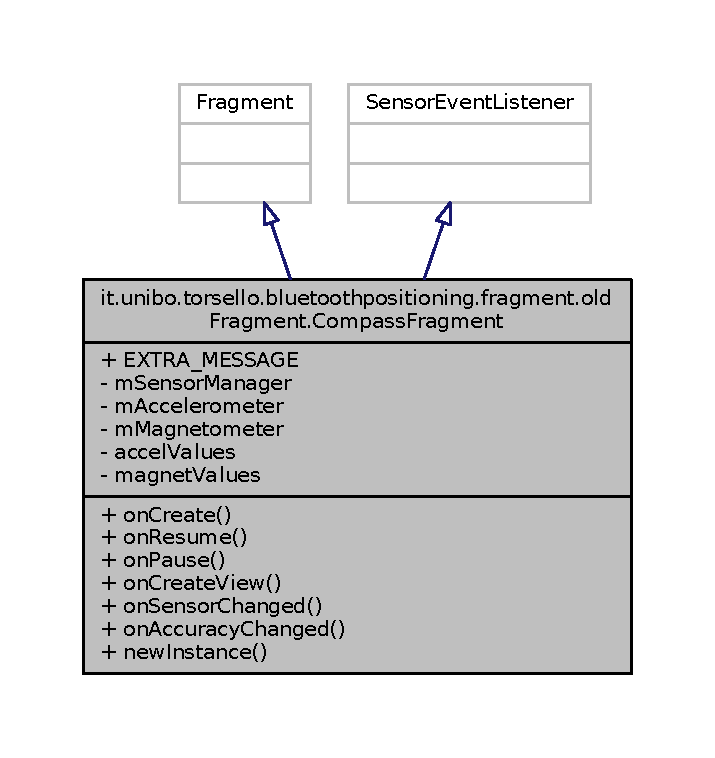
\includegraphics[width=343pt]{classit_1_1unibo_1_1torsello_1_1bluetoothpositioning_1_1fragment_1_1oldFragment_1_1CompassFragment__inherit__graph}
\end{center}
\end{figure}


Diagramma di collaborazione per it.\+unibo.\+torsello.\+bluetoothpositioning.\+fragment.\+old\+Fragment.\+Compass\+Fragment\+:
\nopagebreak
\begin{figure}[H]
\begin{center}
\leavevmode
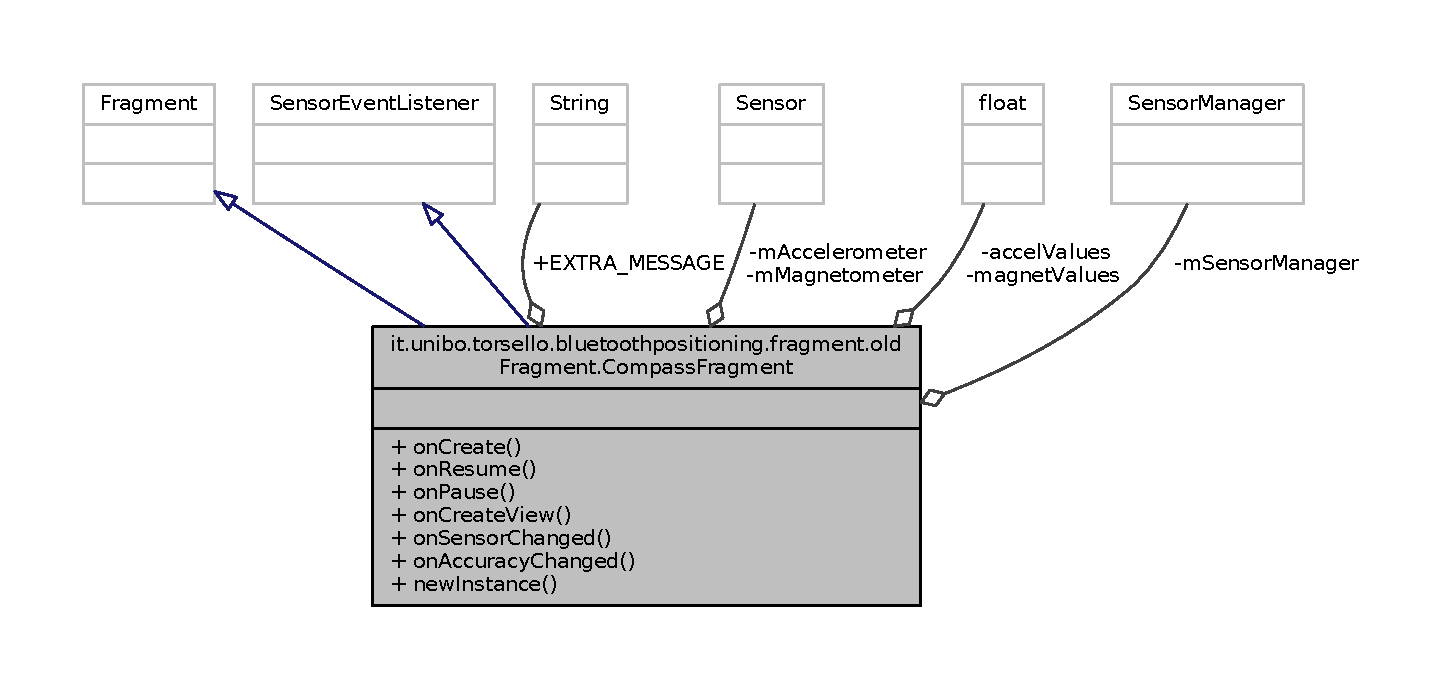
\includegraphics[width=350pt]{classit_1_1unibo_1_1torsello_1_1bluetoothpositioning_1_1fragment_1_1oldFragment_1_1CompassFragment__coll__graph}
\end{center}
\end{figure}
\subsubsection*{Membri pubblici}
\begin{DoxyCompactItemize}
\item 
void \hyperlink{classit_1_1unibo_1_1torsello_1_1bluetoothpositioning_1_1fragment_1_1oldFragment_1_1CompassFragment_aa5fc14a2e767999f225aa4d4b2bff424_aa5fc14a2e767999f225aa4d4b2bff424}{on\+Create} (Bundle saved\+Instance\+State)
\item 
void \hyperlink{classit_1_1unibo_1_1torsello_1_1bluetoothpositioning_1_1fragment_1_1oldFragment_1_1CompassFragment_a32aa07ca1beb0091037267d8d56b9bb2_a32aa07ca1beb0091037267d8d56b9bb2}{on\+Resume} ()
\item 
void \hyperlink{classit_1_1unibo_1_1torsello_1_1bluetoothpositioning_1_1fragment_1_1oldFragment_1_1CompassFragment_a7f6236f3d95a9279e0c58e88aa2401ed_a7f6236f3d95a9279e0c58e88aa2401ed}{on\+Pause} ()
\item 
View \hyperlink{classit_1_1unibo_1_1torsello_1_1bluetoothpositioning_1_1fragment_1_1oldFragment_1_1CompassFragment_ad0f88e0af547fa37b29081074023effb_ad0f88e0af547fa37b29081074023effb}{on\+Create\+View} (Layout\+Inflater inflater, View\+Group container, Bundle saved\+Instance\+State)
\item 
void \hyperlink{classit_1_1unibo_1_1torsello_1_1bluetoothpositioning_1_1fragment_1_1oldFragment_1_1CompassFragment_aadc7f58d3eae6662db5b5ad05a6fd760_aadc7f58d3eae6662db5b5ad05a6fd760}{on\+Sensor\+Changed} (Sensor\+Event event)
\item 
void \hyperlink{classit_1_1unibo_1_1torsello_1_1bluetoothpositioning_1_1fragment_1_1oldFragment_1_1CompassFragment_a72278751498e147f3d18234c884b0490_a72278751498e147f3d18234c884b0490}{on\+Accuracy\+Changed} (Sensor sensor, int accuracy)
\end{DoxyCompactItemize}
\subsubsection*{Membri pubblici statici}
\begin{DoxyCompactItemize}
\item 
static \hyperlink{classit_1_1unibo_1_1torsello_1_1bluetoothpositioning_1_1fragment_1_1oldFragment_1_1CompassFragment}{Compass\+Fragment} \hyperlink{classit_1_1unibo_1_1torsello_1_1bluetoothpositioning_1_1fragment_1_1oldFragment_1_1CompassFragment_a679cc6d37eb185a303b003939ea92b7b_a679cc6d37eb185a303b003939ea92b7b}{new\+Instance} (String message)
\end{DoxyCompactItemize}
\subsubsection*{Attributi pubblici statici}
\begin{DoxyCompactItemize}
\item 
static final String \hyperlink{classit_1_1unibo_1_1torsello_1_1bluetoothpositioning_1_1fragment_1_1oldFragment_1_1CompassFragment_aa984dd2435af48bbcb21cafa07f8e16a_aa984dd2435af48bbcb21cafa07f8e16a}{E\+X\+T\+R\+A\+\_\+\+M\+E\+S\+S\+A\+GE} = \char`\"{}E\+X\+T\+R\+A\+\_\+\+M\+E\+S\+S\+A\+GE\char`\"{}
\end{DoxyCompactItemize}
\subsubsection*{Attributi privati}
\begin{DoxyCompactItemize}
\item 
Sensor\+Manager \hyperlink{classit_1_1unibo_1_1torsello_1_1bluetoothpositioning_1_1fragment_1_1oldFragment_1_1CompassFragment_a9006c75f41300481eaa95c6bb02143e3_a9006c75f41300481eaa95c6bb02143e3}{m\+Sensor\+Manager}
\item 
Sensor \hyperlink{classit_1_1unibo_1_1torsello_1_1bluetoothpositioning_1_1fragment_1_1oldFragment_1_1CompassFragment_a9f521d80f0f7b0e89bb26951c2e463c0_a9f521d80f0f7b0e89bb26951c2e463c0}{m\+Accelerometer}
\item 
Sensor \hyperlink{classit_1_1unibo_1_1torsello_1_1bluetoothpositioning_1_1fragment_1_1oldFragment_1_1CompassFragment_a9e3cd0081d45a26094a8395fe67736c6_a9e3cd0081d45a26094a8395fe67736c6}{m\+Magnetometer}
\item 
float \hyperlink{classit_1_1unibo_1_1torsello_1_1bluetoothpositioning_1_1fragment_1_1oldFragment_1_1CompassFragment_a001321cd7ff2955f1ab00b840a477281_a001321cd7ff2955f1ab00b840a477281}{accel\+Values} \mbox{[}$\,$\mbox{]}
\item 
float \hyperlink{classit_1_1unibo_1_1torsello_1_1bluetoothpositioning_1_1fragment_1_1oldFragment_1_1CompassFragment_a202e7056f07b065dd96894de79faa0a4_a202e7056f07b065dd96894de79faa0a4}{magnet\+Values} \mbox{[}$\,$\mbox{]}
\end{DoxyCompactItemize}


\subsubsection{Descrizione dettagliata}
Created by Federico Torsello. \href{mailto:federico.torsello@studio.unibo.it}{\tt federico.\+torsello@studio.\+unibo.\+it} 

\subsubsection{Documentazione delle funzioni membro}
\hypertarget{classit_1_1unibo_1_1torsello_1_1bluetoothpositioning_1_1fragment_1_1oldFragment_1_1CompassFragment_a679cc6d37eb185a303b003939ea92b7b_a679cc6d37eb185a303b003939ea92b7b}{}\label{classit_1_1unibo_1_1torsello_1_1bluetoothpositioning_1_1fragment_1_1oldFragment_1_1CompassFragment_a679cc6d37eb185a303b003939ea92b7b_a679cc6d37eb185a303b003939ea92b7b} 
\index{it\+::unibo\+::torsello\+::bluetoothpositioning\+::fragment\+::old\+Fragment\+::\+Compass\+Fragment@{it\+::unibo\+::torsello\+::bluetoothpositioning\+::fragment\+::old\+Fragment\+::\+Compass\+Fragment}!new\+Instance@{new\+Instance}}
\index{new\+Instance@{new\+Instance}!it\+::unibo\+::torsello\+::bluetoothpositioning\+::fragment\+::old\+Fragment\+::\+Compass\+Fragment@{it\+::unibo\+::torsello\+::bluetoothpositioning\+::fragment\+::old\+Fragment\+::\+Compass\+Fragment}}
\paragraph{\texorpdfstring{new\+Instance()}{newInstance()}}
{\footnotesize\ttfamily static \hyperlink{classit_1_1unibo_1_1torsello_1_1bluetoothpositioning_1_1fragment_1_1oldFragment_1_1CompassFragment}{Compass\+Fragment} it.\+unibo.\+torsello.\+bluetoothpositioning.\+fragment.\+old\+Fragment.\+Compass\+Fragment.\+new\+Instance (\begin{DoxyParamCaption}\item[{String}]{message }\end{DoxyParamCaption})\hspace{0.3cm}{\ttfamily [static]}}


\begin{DoxyCode}
32                                                               \{
33         CompassFragment fragment = \textcolor{keyword}{new} CompassFragment();
34         Bundle args = \textcolor{keyword}{new} Bundle();
35         args.putString(\hyperlink{classit_1_1unibo_1_1torsello_1_1bluetoothpositioning_1_1fragment_1_1oldFragment_1_1CompassFragment_aa984dd2435af48bbcb21cafa07f8e16a_aa984dd2435af48bbcb21cafa07f8e16a}{EXTRA\_MESSAGE}, message);
36         fragment.setArguments(args);
37         \textcolor{keywordflow}{return} fragment;
38     \}
\end{DoxyCode}
\hypertarget{classit_1_1unibo_1_1torsello_1_1bluetoothpositioning_1_1fragment_1_1oldFragment_1_1CompassFragment_a72278751498e147f3d18234c884b0490_a72278751498e147f3d18234c884b0490}{}\label{classit_1_1unibo_1_1torsello_1_1bluetoothpositioning_1_1fragment_1_1oldFragment_1_1CompassFragment_a72278751498e147f3d18234c884b0490_a72278751498e147f3d18234c884b0490} 
\index{it\+::unibo\+::torsello\+::bluetoothpositioning\+::fragment\+::old\+Fragment\+::\+Compass\+Fragment@{it\+::unibo\+::torsello\+::bluetoothpositioning\+::fragment\+::old\+Fragment\+::\+Compass\+Fragment}!on\+Accuracy\+Changed@{on\+Accuracy\+Changed}}
\index{on\+Accuracy\+Changed@{on\+Accuracy\+Changed}!it\+::unibo\+::torsello\+::bluetoothpositioning\+::fragment\+::old\+Fragment\+::\+Compass\+Fragment@{it\+::unibo\+::torsello\+::bluetoothpositioning\+::fragment\+::old\+Fragment\+::\+Compass\+Fragment}}
\paragraph{\texorpdfstring{on\+Accuracy\+Changed()}{onAccuracyChanged()}}
{\footnotesize\ttfamily void it.\+unibo.\+torsello.\+bluetoothpositioning.\+fragment.\+old\+Fragment.\+Compass\+Fragment.\+on\+Accuracy\+Changed (\begin{DoxyParamCaption}\item[{Sensor}]{sensor,  }\item[{int}]{accuracy }\end{DoxyParamCaption})}


\begin{DoxyCode}
118                                                                \{
119     \}
\end{DoxyCode}
\hypertarget{classit_1_1unibo_1_1torsello_1_1bluetoothpositioning_1_1fragment_1_1oldFragment_1_1CompassFragment_aa5fc14a2e767999f225aa4d4b2bff424_aa5fc14a2e767999f225aa4d4b2bff424}{}\label{classit_1_1unibo_1_1torsello_1_1bluetoothpositioning_1_1fragment_1_1oldFragment_1_1CompassFragment_aa5fc14a2e767999f225aa4d4b2bff424_aa5fc14a2e767999f225aa4d4b2bff424} 
\index{it\+::unibo\+::torsello\+::bluetoothpositioning\+::fragment\+::old\+Fragment\+::\+Compass\+Fragment@{it\+::unibo\+::torsello\+::bluetoothpositioning\+::fragment\+::old\+Fragment\+::\+Compass\+Fragment}!on\+Create@{on\+Create}}
\index{on\+Create@{on\+Create}!it\+::unibo\+::torsello\+::bluetoothpositioning\+::fragment\+::old\+Fragment\+::\+Compass\+Fragment@{it\+::unibo\+::torsello\+::bluetoothpositioning\+::fragment\+::old\+Fragment\+::\+Compass\+Fragment}}
\paragraph{\texorpdfstring{on\+Create()}{onCreate()}}
{\footnotesize\ttfamily void it.\+unibo.\+torsello.\+bluetoothpositioning.\+fragment.\+old\+Fragment.\+Compass\+Fragment.\+on\+Create (\begin{DoxyParamCaption}\item[{Bundle}]{saved\+Instance\+State }\end{DoxyParamCaption})}


\begin{DoxyCode}
41                                                     \{
42         super.onCreate(savedInstanceState);
43         \hyperlink{classit_1_1unibo_1_1torsello_1_1bluetoothpositioning_1_1fragment_1_1oldFragment_1_1CompassFragment_a9006c75f41300481eaa95c6bb02143e3_a9006c75f41300481eaa95c6bb02143e3}{mSensorManager} = (SensorManager) getActivity().getSystemService(Context.
      SENSOR\_SERVICE);
44         \hyperlink{classit_1_1unibo_1_1torsello_1_1bluetoothpositioning_1_1fragment_1_1oldFragment_1_1CompassFragment_a9f521d80f0f7b0e89bb26951c2e463c0_a9f521d80f0f7b0e89bb26951c2e463c0}{mAccelerometer} = \hyperlink{classit_1_1unibo_1_1torsello_1_1bluetoothpositioning_1_1fragment_1_1oldFragment_1_1CompassFragment_a9006c75f41300481eaa95c6bb02143e3_a9006c75f41300481eaa95c6bb02143e3}{mSensorManager}.getDefaultSensor(Sensor.
      TYPE\_ACCELEROMETER);
45         \hyperlink{classit_1_1unibo_1_1torsello_1_1bluetoothpositioning_1_1fragment_1_1oldFragment_1_1CompassFragment_a9e3cd0081d45a26094a8395fe67736c6_a9e3cd0081d45a26094a8395fe67736c6}{mMagnetometer} = \hyperlink{classit_1_1unibo_1_1torsello_1_1bluetoothpositioning_1_1fragment_1_1oldFragment_1_1CompassFragment_a9006c75f41300481eaa95c6bb02143e3_a9006c75f41300481eaa95c6bb02143e3}{mSensorManager}.getDefaultSensor(Sensor.
      TYPE\_MAGNETIC\_FIELD);
46     \}
\end{DoxyCode}
\hypertarget{classit_1_1unibo_1_1torsello_1_1bluetoothpositioning_1_1fragment_1_1oldFragment_1_1CompassFragment_ad0f88e0af547fa37b29081074023effb_ad0f88e0af547fa37b29081074023effb}{}\label{classit_1_1unibo_1_1torsello_1_1bluetoothpositioning_1_1fragment_1_1oldFragment_1_1CompassFragment_ad0f88e0af547fa37b29081074023effb_ad0f88e0af547fa37b29081074023effb} 
\index{it\+::unibo\+::torsello\+::bluetoothpositioning\+::fragment\+::old\+Fragment\+::\+Compass\+Fragment@{it\+::unibo\+::torsello\+::bluetoothpositioning\+::fragment\+::old\+Fragment\+::\+Compass\+Fragment}!on\+Create\+View@{on\+Create\+View}}
\index{on\+Create\+View@{on\+Create\+View}!it\+::unibo\+::torsello\+::bluetoothpositioning\+::fragment\+::old\+Fragment\+::\+Compass\+Fragment@{it\+::unibo\+::torsello\+::bluetoothpositioning\+::fragment\+::old\+Fragment\+::\+Compass\+Fragment}}
\paragraph{\texorpdfstring{on\+Create\+View()}{onCreateView()}}
{\footnotesize\ttfamily View it.\+unibo.\+torsello.\+bluetoothpositioning.\+fragment.\+old\+Fragment.\+Compass\+Fragment.\+on\+Create\+View (\begin{DoxyParamCaption}\item[{Layout\+Inflater}]{inflater,  }\item[{View\+Group}]{container,  }\item[{Bundle}]{saved\+Instance\+State }\end{DoxyParamCaption})}


\begin{DoxyCode}
78                                                         \{
79         \textcolor{keywordflow}{return} inflater.inflate(R.layout.fragment\_compass, container, \textcolor{keyword}{false});
80     \}
\end{DoxyCode}
\hypertarget{classit_1_1unibo_1_1torsello_1_1bluetoothpositioning_1_1fragment_1_1oldFragment_1_1CompassFragment_a7f6236f3d95a9279e0c58e88aa2401ed_a7f6236f3d95a9279e0c58e88aa2401ed}{}\label{classit_1_1unibo_1_1torsello_1_1bluetoothpositioning_1_1fragment_1_1oldFragment_1_1CompassFragment_a7f6236f3d95a9279e0c58e88aa2401ed_a7f6236f3d95a9279e0c58e88aa2401ed} 
\index{it\+::unibo\+::torsello\+::bluetoothpositioning\+::fragment\+::old\+Fragment\+::\+Compass\+Fragment@{it\+::unibo\+::torsello\+::bluetoothpositioning\+::fragment\+::old\+Fragment\+::\+Compass\+Fragment}!on\+Pause@{on\+Pause}}
\index{on\+Pause@{on\+Pause}!it\+::unibo\+::torsello\+::bluetoothpositioning\+::fragment\+::old\+Fragment\+::\+Compass\+Fragment@{it\+::unibo\+::torsello\+::bluetoothpositioning\+::fragment\+::old\+Fragment\+::\+Compass\+Fragment}}
\paragraph{\texorpdfstring{on\+Pause()}{onPause()}}
{\footnotesize\ttfamily void it.\+unibo.\+torsello.\+bluetoothpositioning.\+fragment.\+old\+Fragment.\+Compass\+Fragment.\+on\+Pause (\begin{DoxyParamCaption}{ }\end{DoxyParamCaption})}


\begin{DoxyCode}
70                           \{
71         super.onPause();
72         \hyperlink{classit_1_1unibo_1_1torsello_1_1bluetoothpositioning_1_1fragment_1_1oldFragment_1_1CompassFragment_a9006c75f41300481eaa95c6bb02143e3_a9006c75f41300481eaa95c6bb02143e3}{mSensorManager}.unregisterListener(\textcolor{keyword}{this}, \hyperlink{classit_1_1unibo_1_1torsello_1_1bluetoothpositioning_1_1fragment_1_1oldFragment_1_1CompassFragment_a9f521d80f0f7b0e89bb26951c2e463c0_a9f521d80f0f7b0e89bb26951c2e463c0}{mAccelerometer});
73         \hyperlink{classit_1_1unibo_1_1torsello_1_1bluetoothpositioning_1_1fragment_1_1oldFragment_1_1CompassFragment_a9006c75f41300481eaa95c6bb02143e3_a9006c75f41300481eaa95c6bb02143e3}{mSensorManager}.unregisterListener(\textcolor{keyword}{this}, \hyperlink{classit_1_1unibo_1_1torsello_1_1bluetoothpositioning_1_1fragment_1_1oldFragment_1_1CompassFragment_a9e3cd0081d45a26094a8395fe67736c6_a9e3cd0081d45a26094a8395fe67736c6}{mMagnetometer});
74     \}
\end{DoxyCode}
\hypertarget{classit_1_1unibo_1_1torsello_1_1bluetoothpositioning_1_1fragment_1_1oldFragment_1_1CompassFragment_a32aa07ca1beb0091037267d8d56b9bb2_a32aa07ca1beb0091037267d8d56b9bb2}{}\label{classit_1_1unibo_1_1torsello_1_1bluetoothpositioning_1_1fragment_1_1oldFragment_1_1CompassFragment_a32aa07ca1beb0091037267d8d56b9bb2_a32aa07ca1beb0091037267d8d56b9bb2} 
\index{it\+::unibo\+::torsello\+::bluetoothpositioning\+::fragment\+::old\+Fragment\+::\+Compass\+Fragment@{it\+::unibo\+::torsello\+::bluetoothpositioning\+::fragment\+::old\+Fragment\+::\+Compass\+Fragment}!on\+Resume@{on\+Resume}}
\index{on\+Resume@{on\+Resume}!it\+::unibo\+::torsello\+::bluetoothpositioning\+::fragment\+::old\+Fragment\+::\+Compass\+Fragment@{it\+::unibo\+::torsello\+::bluetoothpositioning\+::fragment\+::old\+Fragment\+::\+Compass\+Fragment}}
\paragraph{\texorpdfstring{on\+Resume()}{onResume()}}
{\footnotesize\ttfamily void it.\+unibo.\+torsello.\+bluetoothpositioning.\+fragment.\+old\+Fragment.\+Compass\+Fragment.\+on\+Resume (\begin{DoxyParamCaption}{ }\end{DoxyParamCaption})}


\begin{DoxyCode}
49                            \{
50         super.onResume();
51         \textcolor{keywordflow}{if} (\hyperlink{classit_1_1unibo_1_1torsello_1_1bluetoothpositioning_1_1fragment_1_1oldFragment_1_1CompassFragment_a9f521d80f0f7b0e89bb26951c2e463c0_a9f521d80f0f7b0e89bb26951c2e463c0}{mAccelerometer} != null) \{
52             \textcolor{keywordflow}{if} (Build.VERSION.SDK\_INT >= Build.VERSION\_CODES.KITKAT) \{
53                 \hyperlink{classit_1_1unibo_1_1torsello_1_1bluetoothpositioning_1_1fragment_1_1oldFragment_1_1CompassFragment_a9006c75f41300481eaa95c6bb02143e3_a9006c75f41300481eaa95c6bb02143e3}{mSensorManager}.registerListener(\textcolor{keyword}{this}, 
      \hyperlink{classit_1_1unibo_1_1torsello_1_1bluetoothpositioning_1_1fragment_1_1oldFragment_1_1CompassFragment_a9f521d80f0f7b0e89bb26951c2e463c0_a9f521d80f0f7b0e89bb26951c2e463c0}{mAccelerometer}, SensorManager.SENSOR\_DELAY\_FASTEST,
54                         SensorManager.SENSOR\_STATUS\_ACCURACY\_HIGH);
55             \} \textcolor{keywordflow}{else} \{
56                 \hyperlink{classit_1_1unibo_1_1torsello_1_1bluetoothpositioning_1_1fragment_1_1oldFragment_1_1CompassFragment_a9006c75f41300481eaa95c6bb02143e3_a9006c75f41300481eaa95c6bb02143e3}{mSensorManager}.registerListener(\textcolor{keyword}{this}, 
      \hyperlink{classit_1_1unibo_1_1torsello_1_1bluetoothpositioning_1_1fragment_1_1oldFragment_1_1CompassFragment_a9f521d80f0f7b0e89bb26951c2e463c0_a9f521d80f0f7b0e89bb26951c2e463c0}{mAccelerometer}, SensorManager.SENSOR\_DELAY\_FASTEST);
57             \}
58         \}
59 
60         \textcolor{keywordflow}{if} (\hyperlink{classit_1_1unibo_1_1torsello_1_1bluetoothpositioning_1_1fragment_1_1oldFragment_1_1CompassFragment_a9e3cd0081d45a26094a8395fe67736c6_a9e3cd0081d45a26094a8395fe67736c6}{mMagnetometer} != null) \{
61             \textcolor{keywordflow}{if} (Build.VERSION.SDK\_INT >= Build.VERSION\_CODES.KITKAT) \{
62                 \hyperlink{classit_1_1unibo_1_1torsello_1_1bluetoothpositioning_1_1fragment_1_1oldFragment_1_1CompassFragment_a9006c75f41300481eaa95c6bb02143e3_a9006c75f41300481eaa95c6bb02143e3}{mSensorManager}.registerListener(\textcolor{keyword}{this}, 
      \hyperlink{classit_1_1unibo_1_1torsello_1_1bluetoothpositioning_1_1fragment_1_1oldFragment_1_1CompassFragment_a9e3cd0081d45a26094a8395fe67736c6_a9e3cd0081d45a26094a8395fe67736c6}{mMagnetometer}, SensorManager.SENSOR\_DELAY\_FASTEST,
63                         SensorManager.SENSOR\_STATUS\_ACCURACY\_HIGH);
64             \} \textcolor{keywordflow}{else} \{
65                 \hyperlink{classit_1_1unibo_1_1torsello_1_1bluetoothpositioning_1_1fragment_1_1oldFragment_1_1CompassFragment_a9006c75f41300481eaa95c6bb02143e3_a9006c75f41300481eaa95c6bb02143e3}{mSensorManager}.registerListener(\textcolor{keyword}{this}, 
      \hyperlink{classit_1_1unibo_1_1torsello_1_1bluetoothpositioning_1_1fragment_1_1oldFragment_1_1CompassFragment_a9e3cd0081d45a26094a8395fe67736c6_a9e3cd0081d45a26094a8395fe67736c6}{mMagnetometer}, SensorManager.SENSOR\_DELAY\_FASTEST);
66             \}
67         \}
68     \}
\end{DoxyCode}
\hypertarget{classit_1_1unibo_1_1torsello_1_1bluetoothpositioning_1_1fragment_1_1oldFragment_1_1CompassFragment_aadc7f58d3eae6662db5b5ad05a6fd760_aadc7f58d3eae6662db5b5ad05a6fd760}{}\label{classit_1_1unibo_1_1torsello_1_1bluetoothpositioning_1_1fragment_1_1oldFragment_1_1CompassFragment_aadc7f58d3eae6662db5b5ad05a6fd760_aadc7f58d3eae6662db5b5ad05a6fd760} 
\index{it\+::unibo\+::torsello\+::bluetoothpositioning\+::fragment\+::old\+Fragment\+::\+Compass\+Fragment@{it\+::unibo\+::torsello\+::bluetoothpositioning\+::fragment\+::old\+Fragment\+::\+Compass\+Fragment}!on\+Sensor\+Changed@{on\+Sensor\+Changed}}
\index{on\+Sensor\+Changed@{on\+Sensor\+Changed}!it\+::unibo\+::torsello\+::bluetoothpositioning\+::fragment\+::old\+Fragment\+::\+Compass\+Fragment@{it\+::unibo\+::torsello\+::bluetoothpositioning\+::fragment\+::old\+Fragment\+::\+Compass\+Fragment}}
\paragraph{\texorpdfstring{on\+Sensor\+Changed()}{onSensorChanged()}}
{\footnotesize\ttfamily void it.\+unibo.\+torsello.\+bluetoothpositioning.\+fragment.\+old\+Fragment.\+Compass\+Fragment.\+on\+Sensor\+Changed (\begin{DoxyParamCaption}\item[{Sensor\+Event}]{event }\end{DoxyParamCaption})}


\begin{DoxyCode}
83                                                    \{
84         \textcolor{keywordflow}{if} (event.sensor == \hyperlink{classit_1_1unibo_1_1torsello_1_1bluetoothpositioning_1_1fragment_1_1oldFragment_1_1CompassFragment_a9f521d80f0f7b0e89bb26951c2e463c0_a9f521d80f0f7b0e89bb26951c2e463c0}{mAccelerometer}) \{
85             \hyperlink{classit_1_1unibo_1_1torsello_1_1bluetoothpositioning_1_1fragment_1_1oldFragment_1_1CompassFragment_a001321cd7ff2955f1ab00b840a477281_a001321cd7ff2955f1ab00b840a477281}{accelValues} = \textcolor{keyword}{event}.values;
86         \} \textcolor{keywordflow}{else} \textcolor{keywordflow}{if} (event.sensor == \hyperlink{classit_1_1unibo_1_1torsello_1_1bluetoothpositioning_1_1fragment_1_1oldFragment_1_1CompassFragment_a9e3cd0081d45a26094a8395fe67736c6_a9e3cd0081d45a26094a8395fe67736c6}{mMagnetometer}) \{
87             \hyperlink{classit_1_1unibo_1_1torsello_1_1bluetoothpositioning_1_1fragment_1_1oldFragment_1_1CompassFragment_a202e7056f07b065dd96894de79faa0a4_a202e7056f07b065dd96894de79faa0a4}{magnetValues} = \textcolor{keyword}{event}.values;
88         \}
89 
90         \textcolor{keywordflow}{if} (\hyperlink{classit_1_1unibo_1_1torsello_1_1bluetoothpositioning_1_1fragment_1_1oldFragment_1_1CompassFragment_a001321cd7ff2955f1ab00b840a477281_a001321cd7ff2955f1ab00b840a477281}{accelValues} != null && \hyperlink{classit_1_1unibo_1_1torsello_1_1bluetoothpositioning_1_1fragment_1_1oldFragment_1_1CompassFragment_a202e7056f07b065dd96894de79faa0a4_a202e7056f07b065dd96894de79faa0a4}{magnetValues} != null) \{
91             \textcolor{keywordtype}{float}[] rotationMatrix = \textcolor{keyword}{new} \textcolor{keywordtype}{float}[16];
92             \textcolor{keywordtype}{float}[] orientation = \textcolor{keyword}{new} \textcolor{keywordtype}{float}[16];
93 
94             SensorManager.getRotationMatrix(rotationMatrix, null, \hyperlink{classit_1_1unibo_1_1torsello_1_1bluetoothpositioning_1_1fragment_1_1oldFragment_1_1CompassFragment_a001321cd7ff2955f1ab00b840a477281_a001321cd7ff2955f1ab00b840a477281}{accelValues}, 
      \hyperlink{classit_1_1unibo_1_1torsello_1_1bluetoothpositioning_1_1fragment_1_1oldFragment_1_1CompassFragment_a202e7056f07b065dd96894de79faa0a4_a202e7056f07b065dd96894de79faa0a4}{magnetValues});
95             SensorManager.getOrientation(rotationMatrix, orientation);
96 
97             \textcolor{keywordtype}{float} azimuthDegree = (float) Math.toDegrees(-orientation[0]);
98 
99             RotateAnimation rotateAnimation = \textcolor{keyword}{new} RotateAnimation(
100                     azimuthDegree, azimuthDegree,
101                     Animation.RELATIVE\_TO\_SELF, 0.5f,
102                     Animation.RELATIVE\_TO\_SELF, 0.5f);
103             rotateAnimation.setDuration(250);
104             rotateAnimation.setFillAfter(\textcolor{keyword}{true});
105 
106 
107             \textcolor{keywordflow}{try} \{
108                 ImageView mPointer = (ImageView) getActivity().findViewById(R.id.pointer);
109                 mPointer.startAnimation(rotateAnimation);
110             \} \textcolor{keywordflow}{catch} (NullPointerException e) \{
111                 e.getStackTrace();
112             \}
113         \}
114 
115     \}
\end{DoxyCode}


\subsubsection{Documentazione dei membri dato}
\hypertarget{classit_1_1unibo_1_1torsello_1_1bluetoothpositioning_1_1fragment_1_1oldFragment_1_1CompassFragment_a001321cd7ff2955f1ab00b840a477281_a001321cd7ff2955f1ab00b840a477281}{}\label{classit_1_1unibo_1_1torsello_1_1bluetoothpositioning_1_1fragment_1_1oldFragment_1_1CompassFragment_a001321cd7ff2955f1ab00b840a477281_a001321cd7ff2955f1ab00b840a477281} 
\index{it\+::unibo\+::torsello\+::bluetoothpositioning\+::fragment\+::old\+Fragment\+::\+Compass\+Fragment@{it\+::unibo\+::torsello\+::bluetoothpositioning\+::fragment\+::old\+Fragment\+::\+Compass\+Fragment}!accel\+Values@{accel\+Values}}
\index{accel\+Values@{accel\+Values}!it\+::unibo\+::torsello\+::bluetoothpositioning\+::fragment\+::old\+Fragment\+::\+Compass\+Fragment@{it\+::unibo\+::torsello\+::bluetoothpositioning\+::fragment\+::old\+Fragment\+::\+Compass\+Fragment}}
\paragraph{\texorpdfstring{accel\+Values}{accelValues}}
{\footnotesize\ttfamily float it.\+unibo.\+torsello.\+bluetoothpositioning.\+fragment.\+old\+Fragment.\+Compass\+Fragment.\+accel\+Values\mbox{[}$\,$\mbox{]}\hspace{0.3cm}{\ttfamily [private]}}

\hypertarget{classit_1_1unibo_1_1torsello_1_1bluetoothpositioning_1_1fragment_1_1oldFragment_1_1CompassFragment_aa984dd2435af48bbcb21cafa07f8e16a_aa984dd2435af48bbcb21cafa07f8e16a}{}\label{classit_1_1unibo_1_1torsello_1_1bluetoothpositioning_1_1fragment_1_1oldFragment_1_1CompassFragment_aa984dd2435af48bbcb21cafa07f8e16a_aa984dd2435af48bbcb21cafa07f8e16a} 
\index{it\+::unibo\+::torsello\+::bluetoothpositioning\+::fragment\+::old\+Fragment\+::\+Compass\+Fragment@{it\+::unibo\+::torsello\+::bluetoothpositioning\+::fragment\+::old\+Fragment\+::\+Compass\+Fragment}!E\+X\+T\+R\+A\+\_\+\+M\+E\+S\+S\+A\+GE@{E\+X\+T\+R\+A\+\_\+\+M\+E\+S\+S\+A\+GE}}
\index{E\+X\+T\+R\+A\+\_\+\+M\+E\+S\+S\+A\+GE@{E\+X\+T\+R\+A\+\_\+\+M\+E\+S\+S\+A\+GE}!it\+::unibo\+::torsello\+::bluetoothpositioning\+::fragment\+::old\+Fragment\+::\+Compass\+Fragment@{it\+::unibo\+::torsello\+::bluetoothpositioning\+::fragment\+::old\+Fragment\+::\+Compass\+Fragment}}
\paragraph{\texorpdfstring{E\+X\+T\+R\+A\+\_\+\+M\+E\+S\+S\+A\+GE}{EXTRA\_MESSAGE}}
{\footnotesize\ttfamily final String it.\+unibo.\+torsello.\+bluetoothpositioning.\+fragment.\+old\+Fragment.\+Compass\+Fragment.\+E\+X\+T\+R\+A\+\_\+\+M\+E\+S\+S\+A\+GE = \char`\"{}E\+X\+T\+R\+A\+\_\+\+M\+E\+S\+S\+A\+GE\char`\"{}\hspace{0.3cm}{\ttfamily [static]}}

\hypertarget{classit_1_1unibo_1_1torsello_1_1bluetoothpositioning_1_1fragment_1_1oldFragment_1_1CompassFragment_a9f521d80f0f7b0e89bb26951c2e463c0_a9f521d80f0f7b0e89bb26951c2e463c0}{}\label{classit_1_1unibo_1_1torsello_1_1bluetoothpositioning_1_1fragment_1_1oldFragment_1_1CompassFragment_a9f521d80f0f7b0e89bb26951c2e463c0_a9f521d80f0f7b0e89bb26951c2e463c0} 
\index{it\+::unibo\+::torsello\+::bluetoothpositioning\+::fragment\+::old\+Fragment\+::\+Compass\+Fragment@{it\+::unibo\+::torsello\+::bluetoothpositioning\+::fragment\+::old\+Fragment\+::\+Compass\+Fragment}!m\+Accelerometer@{m\+Accelerometer}}
\index{m\+Accelerometer@{m\+Accelerometer}!it\+::unibo\+::torsello\+::bluetoothpositioning\+::fragment\+::old\+Fragment\+::\+Compass\+Fragment@{it\+::unibo\+::torsello\+::bluetoothpositioning\+::fragment\+::old\+Fragment\+::\+Compass\+Fragment}}
\paragraph{\texorpdfstring{m\+Accelerometer}{mAccelerometer}}
{\footnotesize\ttfamily Sensor it.\+unibo.\+torsello.\+bluetoothpositioning.\+fragment.\+old\+Fragment.\+Compass\+Fragment.\+m\+Accelerometer\hspace{0.3cm}{\ttfamily [private]}}

\hypertarget{classit_1_1unibo_1_1torsello_1_1bluetoothpositioning_1_1fragment_1_1oldFragment_1_1CompassFragment_a202e7056f07b065dd96894de79faa0a4_a202e7056f07b065dd96894de79faa0a4}{}\label{classit_1_1unibo_1_1torsello_1_1bluetoothpositioning_1_1fragment_1_1oldFragment_1_1CompassFragment_a202e7056f07b065dd96894de79faa0a4_a202e7056f07b065dd96894de79faa0a4} 
\index{it\+::unibo\+::torsello\+::bluetoothpositioning\+::fragment\+::old\+Fragment\+::\+Compass\+Fragment@{it\+::unibo\+::torsello\+::bluetoothpositioning\+::fragment\+::old\+Fragment\+::\+Compass\+Fragment}!magnet\+Values@{magnet\+Values}}
\index{magnet\+Values@{magnet\+Values}!it\+::unibo\+::torsello\+::bluetoothpositioning\+::fragment\+::old\+Fragment\+::\+Compass\+Fragment@{it\+::unibo\+::torsello\+::bluetoothpositioning\+::fragment\+::old\+Fragment\+::\+Compass\+Fragment}}
\paragraph{\texorpdfstring{magnet\+Values}{magnetValues}}
{\footnotesize\ttfamily float it.\+unibo.\+torsello.\+bluetoothpositioning.\+fragment.\+old\+Fragment.\+Compass\+Fragment.\+magnet\+Values\mbox{[}$\,$\mbox{]}\hspace{0.3cm}{\ttfamily [private]}}

\hypertarget{classit_1_1unibo_1_1torsello_1_1bluetoothpositioning_1_1fragment_1_1oldFragment_1_1CompassFragment_a9e3cd0081d45a26094a8395fe67736c6_a9e3cd0081d45a26094a8395fe67736c6}{}\label{classit_1_1unibo_1_1torsello_1_1bluetoothpositioning_1_1fragment_1_1oldFragment_1_1CompassFragment_a9e3cd0081d45a26094a8395fe67736c6_a9e3cd0081d45a26094a8395fe67736c6} 
\index{it\+::unibo\+::torsello\+::bluetoothpositioning\+::fragment\+::old\+Fragment\+::\+Compass\+Fragment@{it\+::unibo\+::torsello\+::bluetoothpositioning\+::fragment\+::old\+Fragment\+::\+Compass\+Fragment}!m\+Magnetometer@{m\+Magnetometer}}
\index{m\+Magnetometer@{m\+Magnetometer}!it\+::unibo\+::torsello\+::bluetoothpositioning\+::fragment\+::old\+Fragment\+::\+Compass\+Fragment@{it\+::unibo\+::torsello\+::bluetoothpositioning\+::fragment\+::old\+Fragment\+::\+Compass\+Fragment}}
\paragraph{\texorpdfstring{m\+Magnetometer}{mMagnetometer}}
{\footnotesize\ttfamily Sensor it.\+unibo.\+torsello.\+bluetoothpositioning.\+fragment.\+old\+Fragment.\+Compass\+Fragment.\+m\+Magnetometer\hspace{0.3cm}{\ttfamily [private]}}

\hypertarget{classit_1_1unibo_1_1torsello_1_1bluetoothpositioning_1_1fragment_1_1oldFragment_1_1CompassFragment_a9006c75f41300481eaa95c6bb02143e3_a9006c75f41300481eaa95c6bb02143e3}{}\label{classit_1_1unibo_1_1torsello_1_1bluetoothpositioning_1_1fragment_1_1oldFragment_1_1CompassFragment_a9006c75f41300481eaa95c6bb02143e3_a9006c75f41300481eaa95c6bb02143e3} 
\index{it\+::unibo\+::torsello\+::bluetoothpositioning\+::fragment\+::old\+Fragment\+::\+Compass\+Fragment@{it\+::unibo\+::torsello\+::bluetoothpositioning\+::fragment\+::old\+Fragment\+::\+Compass\+Fragment}!m\+Sensor\+Manager@{m\+Sensor\+Manager}}
\index{m\+Sensor\+Manager@{m\+Sensor\+Manager}!it\+::unibo\+::torsello\+::bluetoothpositioning\+::fragment\+::old\+Fragment\+::\+Compass\+Fragment@{it\+::unibo\+::torsello\+::bluetoothpositioning\+::fragment\+::old\+Fragment\+::\+Compass\+Fragment}}
\paragraph{\texorpdfstring{m\+Sensor\+Manager}{mSensorManager}}
{\footnotesize\ttfamily Sensor\+Manager it.\+unibo.\+torsello.\+bluetoothpositioning.\+fragment.\+old\+Fragment.\+Compass\+Fragment.\+m\+Sensor\+Manager\hspace{0.3cm}{\ttfamily [private]}}



La documentazione per questa classe è stata generata a partire dal seguente file\+:\begin{DoxyCompactItemize}
\item 
\hyperlink{CompassFragment_8java}{Compass\+Fragment.\+java}\end{DoxyCompactItemize}

\hypertarget{classit_1_1unibo_1_1torsello_1_1bluetoothpositioning_1_1fragment_1_1oldFragment_1_1CompassMagnoFragment}{}\subsection{Riferimenti per la classe it.\+unibo.\+torsello.\+bluetoothpositioning.\+fragment.\+old\+Fragment.\+Compass\+Magno\+Fragment}
\label{classit_1_1unibo_1_1torsello_1_1bluetoothpositioning_1_1fragment_1_1oldFragment_1_1CompassMagnoFragment}\index{it.\+unibo.\+torsello.\+bluetoothpositioning.\+fragment.\+old\+Fragment.\+Compass\+Magno\+Fragment@{it.\+unibo.\+torsello.\+bluetoothpositioning.\+fragment.\+old\+Fragment.\+Compass\+Magno\+Fragment}}


Diagramma delle classi per it.\+unibo.\+torsello.\+bluetoothpositioning.\+fragment.\+old\+Fragment.\+Compass\+Magno\+Fragment
\nopagebreak
\begin{figure}[H]
\begin{center}
\leavevmode
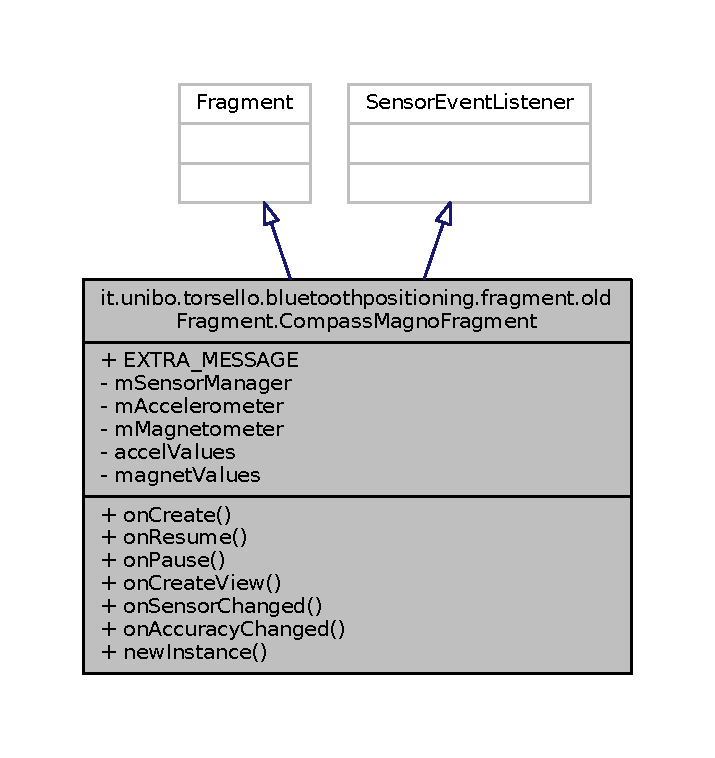
\includegraphics[width=343pt]{classit_1_1unibo_1_1torsello_1_1bluetoothpositioning_1_1fragment_1_1oldFragment_1_1CompassMagnoFragment__inherit__graph}
\end{center}
\end{figure}


Diagramma di collaborazione per it.\+unibo.\+torsello.\+bluetoothpositioning.\+fragment.\+old\+Fragment.\+Compass\+Magno\+Fragment\+:
\nopagebreak
\begin{figure}[H]
\begin{center}
\leavevmode
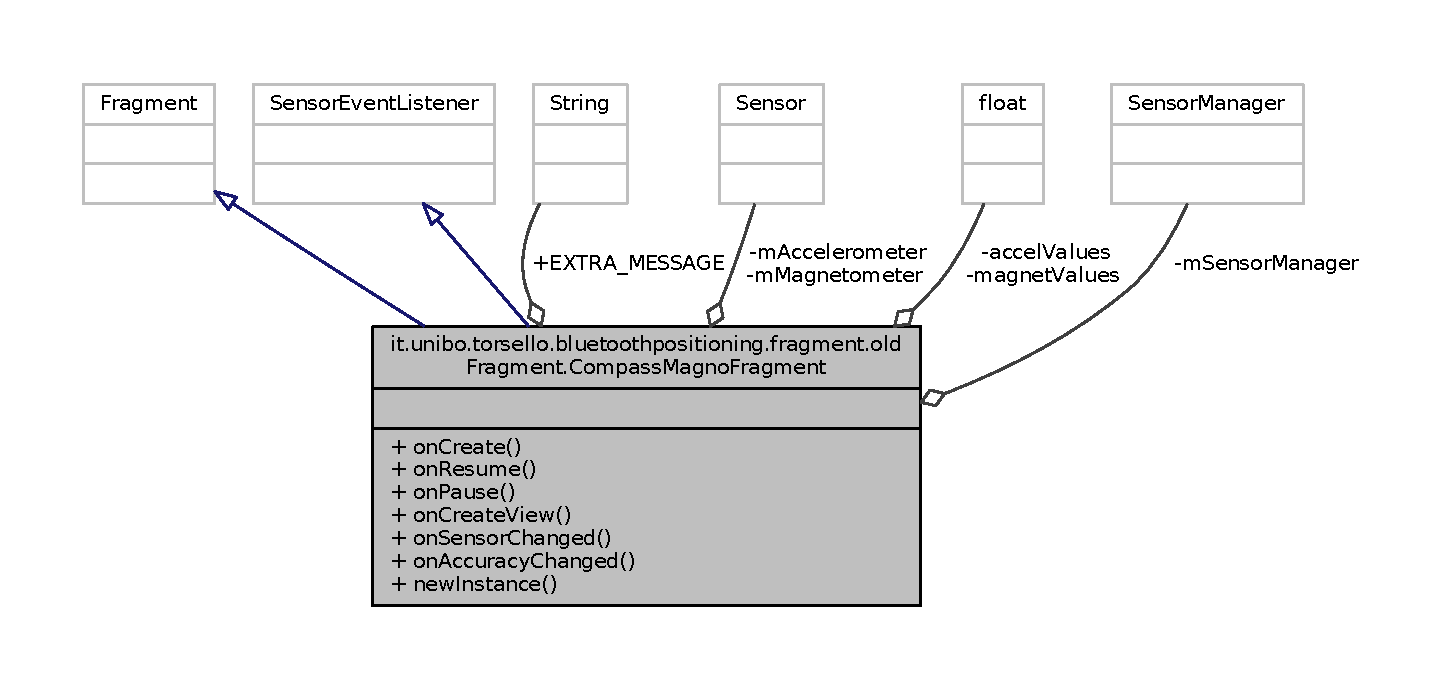
\includegraphics[width=350pt]{classit_1_1unibo_1_1torsello_1_1bluetoothpositioning_1_1fragment_1_1oldFragment_1_1CompassMagnoFragment__coll__graph}
\end{center}
\end{figure}
\subsubsection*{Membri pubblici}
\begin{DoxyCompactItemize}
\item 
void \hyperlink{classit_1_1unibo_1_1torsello_1_1bluetoothpositioning_1_1fragment_1_1oldFragment_1_1CompassMagnoFragment_ac7b5ed11aa2b31a711158c4b7dd1b3ec_ac7b5ed11aa2b31a711158c4b7dd1b3ec}{on\+Create} (@Nullable Bundle saved\+Instance\+State)
\item 
void \hyperlink{classit_1_1unibo_1_1torsello_1_1bluetoothpositioning_1_1fragment_1_1oldFragment_1_1CompassMagnoFragment_a035b99f484588d946d29f417113f0dc2_a035b99f484588d946d29f417113f0dc2}{on\+Resume} ()
\item 
void \hyperlink{classit_1_1unibo_1_1torsello_1_1bluetoothpositioning_1_1fragment_1_1oldFragment_1_1CompassMagnoFragment_a6cf13eaf60004dff28dd71ef75d6d719_a6cf13eaf60004dff28dd71ef75d6d719}{on\+Pause} ()
\item 
View \hyperlink{classit_1_1unibo_1_1torsello_1_1bluetoothpositioning_1_1fragment_1_1oldFragment_1_1CompassMagnoFragment_a3ea35cb229abc119708ab9b559781f45_a3ea35cb229abc119708ab9b559781f45}{on\+Create\+View} (Layout\+Inflater inflater, View\+Group container, Bundle saved\+Instance\+State)
\item 
void \hyperlink{classit_1_1unibo_1_1torsello_1_1bluetoothpositioning_1_1fragment_1_1oldFragment_1_1CompassMagnoFragment_aa18c6b8e8b0e10f5a37032660755a0fa_aa18c6b8e8b0e10f5a37032660755a0fa}{on\+Sensor\+Changed} (Sensor\+Event event)
\item 
void \hyperlink{classit_1_1unibo_1_1torsello_1_1bluetoothpositioning_1_1fragment_1_1oldFragment_1_1CompassMagnoFragment_ab7f5e45a12c41ff850294d67ae54ae4c_ab7f5e45a12c41ff850294d67ae54ae4c}{on\+Accuracy\+Changed} (Sensor sensor, int accuracy)
\end{DoxyCompactItemize}
\subsubsection*{Membri pubblici statici}
\begin{DoxyCompactItemize}
\item 
static \hyperlink{classit_1_1unibo_1_1torsello_1_1bluetoothpositioning_1_1fragment_1_1oldFragment_1_1CompassMagnoFragment}{Compass\+Magno\+Fragment} \hyperlink{classit_1_1unibo_1_1torsello_1_1bluetoothpositioning_1_1fragment_1_1oldFragment_1_1CompassMagnoFragment_a2fdc7669262528be61e2e0165b6a8901_a2fdc7669262528be61e2e0165b6a8901}{new\+Instance} (String message)
\end{DoxyCompactItemize}
\subsubsection*{Attributi pubblici statici}
\begin{DoxyCompactItemize}
\item 
static final String \hyperlink{classit_1_1unibo_1_1torsello_1_1bluetoothpositioning_1_1fragment_1_1oldFragment_1_1CompassMagnoFragment_ad570a334dd03dbb05b6615a4df79e811_ad570a334dd03dbb05b6615a4df79e811}{E\+X\+T\+R\+A\+\_\+\+M\+E\+S\+S\+A\+GE} = \char`\"{}E\+X\+T\+R\+A\+\_\+\+M\+E\+S\+S\+A\+GE\char`\"{}
\end{DoxyCompactItemize}
\subsubsection*{Attributi privati}
\begin{DoxyCompactItemize}
\item 
Sensor\+Manager \hyperlink{classit_1_1unibo_1_1torsello_1_1bluetoothpositioning_1_1fragment_1_1oldFragment_1_1CompassMagnoFragment_ae6b91ce34c58940e5f936dba964d6182_ae6b91ce34c58940e5f936dba964d6182}{m\+Sensor\+Manager}
\item 
Sensor \hyperlink{classit_1_1unibo_1_1torsello_1_1bluetoothpositioning_1_1fragment_1_1oldFragment_1_1CompassMagnoFragment_ae5b2153973fd62a9142fa372461808c5_ae5b2153973fd62a9142fa372461808c5}{m\+Accelerometer}
\item 
Sensor \hyperlink{classit_1_1unibo_1_1torsello_1_1bluetoothpositioning_1_1fragment_1_1oldFragment_1_1CompassMagnoFragment_a7ff1cf69c59de3ce3b93de90501d1848_a7ff1cf69c59de3ce3b93de90501d1848}{m\+Magnetometer}
\item 
float \hyperlink{classit_1_1unibo_1_1torsello_1_1bluetoothpositioning_1_1fragment_1_1oldFragment_1_1CompassMagnoFragment_a6fd163a92ff4354d07d7eefbeed24b62_a6fd163a92ff4354d07d7eefbeed24b62}{accel\+Values} \mbox{[}$\,$\mbox{]}
\item 
float \hyperlink{classit_1_1unibo_1_1torsello_1_1bluetoothpositioning_1_1fragment_1_1oldFragment_1_1CompassMagnoFragment_aa8991b737848cba64dc1ebd397f5a390_aa8991b737848cba64dc1ebd397f5a390}{magnet\+Values} \mbox{[}$\,$\mbox{]}
\end{DoxyCompactItemize}


\subsubsection{Descrizione dettagliata}
Created by Federico Torsello. \href{mailto:federico.torsello@studio.unibo.it}{\tt federico.\+torsello@studio.\+unibo.\+it} 

\subsubsection{Documentazione delle funzioni membro}
\hypertarget{classit_1_1unibo_1_1torsello_1_1bluetoothpositioning_1_1fragment_1_1oldFragment_1_1CompassMagnoFragment_a2fdc7669262528be61e2e0165b6a8901_a2fdc7669262528be61e2e0165b6a8901}{}\label{classit_1_1unibo_1_1torsello_1_1bluetoothpositioning_1_1fragment_1_1oldFragment_1_1CompassMagnoFragment_a2fdc7669262528be61e2e0165b6a8901_a2fdc7669262528be61e2e0165b6a8901} 
\index{it\+::unibo\+::torsello\+::bluetoothpositioning\+::fragment\+::old\+Fragment\+::\+Compass\+Magno\+Fragment@{it\+::unibo\+::torsello\+::bluetoothpositioning\+::fragment\+::old\+Fragment\+::\+Compass\+Magno\+Fragment}!new\+Instance@{new\+Instance}}
\index{new\+Instance@{new\+Instance}!it\+::unibo\+::torsello\+::bluetoothpositioning\+::fragment\+::old\+Fragment\+::\+Compass\+Magno\+Fragment@{it\+::unibo\+::torsello\+::bluetoothpositioning\+::fragment\+::old\+Fragment\+::\+Compass\+Magno\+Fragment}}
\paragraph{\texorpdfstring{new\+Instance()}{newInstance()}}
{\footnotesize\ttfamily static \hyperlink{classit_1_1unibo_1_1torsello_1_1bluetoothpositioning_1_1fragment_1_1oldFragment_1_1CompassMagnoFragment}{Compass\+Magno\+Fragment} it.\+unibo.\+torsello.\+bluetoothpositioning.\+fragment.\+old\+Fragment.\+Compass\+Magno\+Fragment.\+new\+Instance (\begin{DoxyParamCaption}\item[{String}]{message }\end{DoxyParamCaption})\hspace{0.3cm}{\ttfamily [static]}}


\begin{DoxyCode}
30                                                                    \{
31         CompassMagnoFragment fragment = \textcolor{keyword}{new} CompassMagnoFragment();
32         Bundle args = \textcolor{keyword}{new} Bundle();
33         args.putString(\hyperlink{classit_1_1unibo_1_1torsello_1_1bluetoothpositioning_1_1fragment_1_1oldFragment_1_1CompassMagnoFragment_ad570a334dd03dbb05b6615a4df79e811_ad570a334dd03dbb05b6615a4df79e811}{EXTRA\_MESSAGE}, message);
34         fragment.setArguments(args);
35         \textcolor{keywordflow}{return} fragment;
36     \}
\end{DoxyCode}
\hypertarget{classit_1_1unibo_1_1torsello_1_1bluetoothpositioning_1_1fragment_1_1oldFragment_1_1CompassMagnoFragment_ab7f5e45a12c41ff850294d67ae54ae4c_ab7f5e45a12c41ff850294d67ae54ae4c}{}\label{classit_1_1unibo_1_1torsello_1_1bluetoothpositioning_1_1fragment_1_1oldFragment_1_1CompassMagnoFragment_ab7f5e45a12c41ff850294d67ae54ae4c_ab7f5e45a12c41ff850294d67ae54ae4c} 
\index{it\+::unibo\+::torsello\+::bluetoothpositioning\+::fragment\+::old\+Fragment\+::\+Compass\+Magno\+Fragment@{it\+::unibo\+::torsello\+::bluetoothpositioning\+::fragment\+::old\+Fragment\+::\+Compass\+Magno\+Fragment}!on\+Accuracy\+Changed@{on\+Accuracy\+Changed}}
\index{on\+Accuracy\+Changed@{on\+Accuracy\+Changed}!it\+::unibo\+::torsello\+::bluetoothpositioning\+::fragment\+::old\+Fragment\+::\+Compass\+Magno\+Fragment@{it\+::unibo\+::torsello\+::bluetoothpositioning\+::fragment\+::old\+Fragment\+::\+Compass\+Magno\+Fragment}}
\paragraph{\texorpdfstring{on\+Accuracy\+Changed()}{onAccuracyChanged()}}
{\footnotesize\ttfamily void it.\+unibo.\+torsello.\+bluetoothpositioning.\+fragment.\+old\+Fragment.\+Compass\+Magno\+Fragment.\+on\+Accuracy\+Changed (\begin{DoxyParamCaption}\item[{Sensor}]{sensor,  }\item[{int}]{accuracy }\end{DoxyParamCaption})}


\begin{DoxyCode}
126                                                                \{
127 
128     \}
\end{DoxyCode}
\hypertarget{classit_1_1unibo_1_1torsello_1_1bluetoothpositioning_1_1fragment_1_1oldFragment_1_1CompassMagnoFragment_ac7b5ed11aa2b31a711158c4b7dd1b3ec_ac7b5ed11aa2b31a711158c4b7dd1b3ec}{}\label{classit_1_1unibo_1_1torsello_1_1bluetoothpositioning_1_1fragment_1_1oldFragment_1_1CompassMagnoFragment_ac7b5ed11aa2b31a711158c4b7dd1b3ec_ac7b5ed11aa2b31a711158c4b7dd1b3ec} 
\index{it\+::unibo\+::torsello\+::bluetoothpositioning\+::fragment\+::old\+Fragment\+::\+Compass\+Magno\+Fragment@{it\+::unibo\+::torsello\+::bluetoothpositioning\+::fragment\+::old\+Fragment\+::\+Compass\+Magno\+Fragment}!on\+Create@{on\+Create}}
\index{on\+Create@{on\+Create}!it\+::unibo\+::torsello\+::bluetoothpositioning\+::fragment\+::old\+Fragment\+::\+Compass\+Magno\+Fragment@{it\+::unibo\+::torsello\+::bluetoothpositioning\+::fragment\+::old\+Fragment\+::\+Compass\+Magno\+Fragment}}
\paragraph{\texorpdfstring{on\+Create()}{onCreate()}}
{\footnotesize\ttfamily void it.\+unibo.\+torsello.\+bluetoothpositioning.\+fragment.\+old\+Fragment.\+Compass\+Magno\+Fragment.\+on\+Create (\begin{DoxyParamCaption}\item[{@Nullable Bundle}]{saved\+Instance\+State }\end{DoxyParamCaption})}


\begin{DoxyCode}
40                                                               \{
41         super.onCreate(savedInstanceState);
42         setHasOptionsMenu(\textcolor{keyword}{true});
43         \hyperlink{classit_1_1unibo_1_1torsello_1_1bluetoothpositioning_1_1fragment_1_1oldFragment_1_1CompassMagnoFragment_ae6b91ce34c58940e5f936dba964d6182_ae6b91ce34c58940e5f936dba964d6182}{mSensorManager} = (SensorManager) getActivity().getSystemService(Context.
      SENSOR\_SERVICE);
44         \hyperlink{classit_1_1unibo_1_1torsello_1_1bluetoothpositioning_1_1fragment_1_1oldFragment_1_1CompassMagnoFragment_ae5b2153973fd62a9142fa372461808c5_ae5b2153973fd62a9142fa372461808c5}{mAccelerometer} = \hyperlink{classit_1_1unibo_1_1torsello_1_1bluetoothpositioning_1_1fragment_1_1oldFragment_1_1CompassMagnoFragment_ae6b91ce34c58940e5f936dba964d6182_ae6b91ce34c58940e5f936dba964d6182}{mSensorManager}.getDefaultSensor(Sensor.
      TYPE\_ACCELEROMETER);
45         \hyperlink{classit_1_1unibo_1_1torsello_1_1bluetoothpositioning_1_1fragment_1_1oldFragment_1_1CompassMagnoFragment_a7ff1cf69c59de3ce3b93de90501d1848_a7ff1cf69c59de3ce3b93de90501d1848}{mMagnetometer} = \hyperlink{classit_1_1unibo_1_1torsello_1_1bluetoothpositioning_1_1fragment_1_1oldFragment_1_1CompassMagnoFragment_ae6b91ce34c58940e5f936dba964d6182_ae6b91ce34c58940e5f936dba964d6182}{mSensorManager}.getDefaultSensor(Sensor.
      TYPE\_MAGNETIC\_FIELD);
46     \}
\end{DoxyCode}
\hypertarget{classit_1_1unibo_1_1torsello_1_1bluetoothpositioning_1_1fragment_1_1oldFragment_1_1CompassMagnoFragment_a3ea35cb229abc119708ab9b559781f45_a3ea35cb229abc119708ab9b559781f45}{}\label{classit_1_1unibo_1_1torsello_1_1bluetoothpositioning_1_1fragment_1_1oldFragment_1_1CompassMagnoFragment_a3ea35cb229abc119708ab9b559781f45_a3ea35cb229abc119708ab9b559781f45} 
\index{it\+::unibo\+::torsello\+::bluetoothpositioning\+::fragment\+::old\+Fragment\+::\+Compass\+Magno\+Fragment@{it\+::unibo\+::torsello\+::bluetoothpositioning\+::fragment\+::old\+Fragment\+::\+Compass\+Magno\+Fragment}!on\+Create\+View@{on\+Create\+View}}
\index{on\+Create\+View@{on\+Create\+View}!it\+::unibo\+::torsello\+::bluetoothpositioning\+::fragment\+::old\+Fragment\+::\+Compass\+Magno\+Fragment@{it\+::unibo\+::torsello\+::bluetoothpositioning\+::fragment\+::old\+Fragment\+::\+Compass\+Magno\+Fragment}}
\paragraph{\texorpdfstring{on\+Create\+View()}{onCreateView()}}
{\footnotesize\ttfamily View it.\+unibo.\+torsello.\+bluetoothpositioning.\+fragment.\+old\+Fragment.\+Compass\+Magno\+Fragment.\+on\+Create\+View (\begin{DoxyParamCaption}\item[{Layout\+Inflater}]{inflater,  }\item[{View\+Group}]{container,  }\item[{Bundle}]{saved\+Instance\+State }\end{DoxyParamCaption})}


\begin{DoxyCode}
80                                                         \{
81         \textcolor{keywordflow}{return} inflater.inflate(R.layout.fragment\_compass\_text, container, \textcolor{keyword}{false});
82     \}
\end{DoxyCode}
\hypertarget{classit_1_1unibo_1_1torsello_1_1bluetoothpositioning_1_1fragment_1_1oldFragment_1_1CompassMagnoFragment_a6cf13eaf60004dff28dd71ef75d6d719_a6cf13eaf60004dff28dd71ef75d6d719}{}\label{classit_1_1unibo_1_1torsello_1_1bluetoothpositioning_1_1fragment_1_1oldFragment_1_1CompassMagnoFragment_a6cf13eaf60004dff28dd71ef75d6d719_a6cf13eaf60004dff28dd71ef75d6d719} 
\index{it\+::unibo\+::torsello\+::bluetoothpositioning\+::fragment\+::old\+Fragment\+::\+Compass\+Magno\+Fragment@{it\+::unibo\+::torsello\+::bluetoothpositioning\+::fragment\+::old\+Fragment\+::\+Compass\+Magno\+Fragment}!on\+Pause@{on\+Pause}}
\index{on\+Pause@{on\+Pause}!it\+::unibo\+::torsello\+::bluetoothpositioning\+::fragment\+::old\+Fragment\+::\+Compass\+Magno\+Fragment@{it\+::unibo\+::torsello\+::bluetoothpositioning\+::fragment\+::old\+Fragment\+::\+Compass\+Magno\+Fragment}}
\paragraph{\texorpdfstring{on\+Pause()}{onPause()}}
{\footnotesize\ttfamily void it.\+unibo.\+torsello.\+bluetoothpositioning.\+fragment.\+old\+Fragment.\+Compass\+Magno\+Fragment.\+on\+Pause (\begin{DoxyParamCaption}{ }\end{DoxyParamCaption})}


\begin{DoxyCode}
72                           \{
73         super.onPause();
74         \hyperlink{classit_1_1unibo_1_1torsello_1_1bluetoothpositioning_1_1fragment_1_1oldFragment_1_1CompassMagnoFragment_ae6b91ce34c58940e5f936dba964d6182_ae6b91ce34c58940e5f936dba964d6182}{mSensorManager}.unregisterListener(\textcolor{keyword}{this}, \hyperlink{classit_1_1unibo_1_1torsello_1_1bluetoothpositioning_1_1fragment_1_1oldFragment_1_1CompassMagnoFragment_ae5b2153973fd62a9142fa372461808c5_ae5b2153973fd62a9142fa372461808c5}{mAccelerometer});
75         \hyperlink{classit_1_1unibo_1_1torsello_1_1bluetoothpositioning_1_1fragment_1_1oldFragment_1_1CompassMagnoFragment_ae6b91ce34c58940e5f936dba964d6182_ae6b91ce34c58940e5f936dba964d6182}{mSensorManager}.unregisterListener(\textcolor{keyword}{this}, \hyperlink{classit_1_1unibo_1_1torsello_1_1bluetoothpositioning_1_1fragment_1_1oldFragment_1_1CompassMagnoFragment_a7ff1cf69c59de3ce3b93de90501d1848_a7ff1cf69c59de3ce3b93de90501d1848}{mMagnetometer});
76     \}
\end{DoxyCode}
\hypertarget{classit_1_1unibo_1_1torsello_1_1bluetoothpositioning_1_1fragment_1_1oldFragment_1_1CompassMagnoFragment_a035b99f484588d946d29f417113f0dc2_a035b99f484588d946d29f417113f0dc2}{}\label{classit_1_1unibo_1_1torsello_1_1bluetoothpositioning_1_1fragment_1_1oldFragment_1_1CompassMagnoFragment_a035b99f484588d946d29f417113f0dc2_a035b99f484588d946d29f417113f0dc2} 
\index{it\+::unibo\+::torsello\+::bluetoothpositioning\+::fragment\+::old\+Fragment\+::\+Compass\+Magno\+Fragment@{it\+::unibo\+::torsello\+::bluetoothpositioning\+::fragment\+::old\+Fragment\+::\+Compass\+Magno\+Fragment}!on\+Resume@{on\+Resume}}
\index{on\+Resume@{on\+Resume}!it\+::unibo\+::torsello\+::bluetoothpositioning\+::fragment\+::old\+Fragment\+::\+Compass\+Magno\+Fragment@{it\+::unibo\+::torsello\+::bluetoothpositioning\+::fragment\+::old\+Fragment\+::\+Compass\+Magno\+Fragment}}
\paragraph{\texorpdfstring{on\+Resume()}{onResume()}}
{\footnotesize\ttfamily void it.\+unibo.\+torsello.\+bluetoothpositioning.\+fragment.\+old\+Fragment.\+Compass\+Magno\+Fragment.\+on\+Resume (\begin{DoxyParamCaption}{ }\end{DoxyParamCaption})}


\begin{DoxyCode}
49                            \{
50         super.onResume();
51         \textcolor{keywordflow}{if} (\hyperlink{classit_1_1unibo_1_1torsello_1_1bluetoothpositioning_1_1fragment_1_1oldFragment_1_1CompassMagnoFragment_ae5b2153973fd62a9142fa372461808c5_ae5b2153973fd62a9142fa372461808c5}{mAccelerometer} != null) \{
52             \textcolor{keywordflow}{if} (Build.VERSION.SDK\_INT >= Build.VERSION\_CODES.KITKAT) \{
53                 \hyperlink{classit_1_1unibo_1_1torsello_1_1bluetoothpositioning_1_1fragment_1_1oldFragment_1_1CompassMagnoFragment_ae6b91ce34c58940e5f936dba964d6182_ae6b91ce34c58940e5f936dba964d6182}{mSensorManager}.registerListener(\textcolor{keyword}{this}, 
      \hyperlink{classit_1_1unibo_1_1torsello_1_1bluetoothpositioning_1_1fragment_1_1oldFragment_1_1CompassMagnoFragment_ae5b2153973fd62a9142fa372461808c5_ae5b2153973fd62a9142fa372461808c5}{mAccelerometer}, SensorManager.SENSOR\_DELAY\_FASTEST,
54                         SensorManager.SENSOR\_STATUS\_ACCURACY\_HIGH);
55             \} \textcolor{keywordflow}{else} \{
56                 \hyperlink{classit_1_1unibo_1_1torsello_1_1bluetoothpositioning_1_1fragment_1_1oldFragment_1_1CompassMagnoFragment_ae6b91ce34c58940e5f936dba964d6182_ae6b91ce34c58940e5f936dba964d6182}{mSensorManager}.registerListener(\textcolor{keyword}{this}, 
      \hyperlink{classit_1_1unibo_1_1torsello_1_1bluetoothpositioning_1_1fragment_1_1oldFragment_1_1CompassMagnoFragment_ae5b2153973fd62a9142fa372461808c5_ae5b2153973fd62a9142fa372461808c5}{mAccelerometer}, SensorManager.SENSOR\_DELAY\_FASTEST);
57             \}
58         \}
59 
60         \textcolor{keywordflow}{if} (\hyperlink{classit_1_1unibo_1_1torsello_1_1bluetoothpositioning_1_1fragment_1_1oldFragment_1_1CompassMagnoFragment_a7ff1cf69c59de3ce3b93de90501d1848_a7ff1cf69c59de3ce3b93de90501d1848}{mMagnetometer} != null) \{
61             \textcolor{keywordflow}{if} (Build.VERSION.SDK\_INT >= Build.VERSION\_CODES.KITKAT) \{
62                 \hyperlink{classit_1_1unibo_1_1torsello_1_1bluetoothpositioning_1_1fragment_1_1oldFragment_1_1CompassMagnoFragment_ae6b91ce34c58940e5f936dba964d6182_ae6b91ce34c58940e5f936dba964d6182}{mSensorManager}.registerListener(\textcolor{keyword}{this}, 
      \hyperlink{classit_1_1unibo_1_1torsello_1_1bluetoothpositioning_1_1fragment_1_1oldFragment_1_1CompassMagnoFragment_a7ff1cf69c59de3ce3b93de90501d1848_a7ff1cf69c59de3ce3b93de90501d1848}{mMagnetometer}, SensorManager.SENSOR\_DELAY\_FASTEST,
63                         SensorManager.SENSOR\_STATUS\_ACCURACY\_HIGH);
64             \} \textcolor{keywordflow}{else} \{
65                 \hyperlink{classit_1_1unibo_1_1torsello_1_1bluetoothpositioning_1_1fragment_1_1oldFragment_1_1CompassMagnoFragment_ae6b91ce34c58940e5f936dba964d6182_ae6b91ce34c58940e5f936dba964d6182}{mSensorManager}.registerListener(\textcolor{keyword}{this}, 
      \hyperlink{classit_1_1unibo_1_1torsello_1_1bluetoothpositioning_1_1fragment_1_1oldFragment_1_1CompassMagnoFragment_a7ff1cf69c59de3ce3b93de90501d1848_a7ff1cf69c59de3ce3b93de90501d1848}{mMagnetometer}, SensorManager.SENSOR\_DELAY\_FASTEST);
66             \}
67         \}
68     \}
\end{DoxyCode}
\hypertarget{classit_1_1unibo_1_1torsello_1_1bluetoothpositioning_1_1fragment_1_1oldFragment_1_1CompassMagnoFragment_aa18c6b8e8b0e10f5a37032660755a0fa_aa18c6b8e8b0e10f5a37032660755a0fa}{}\label{classit_1_1unibo_1_1torsello_1_1bluetoothpositioning_1_1fragment_1_1oldFragment_1_1CompassMagnoFragment_aa18c6b8e8b0e10f5a37032660755a0fa_aa18c6b8e8b0e10f5a37032660755a0fa} 
\index{it\+::unibo\+::torsello\+::bluetoothpositioning\+::fragment\+::old\+Fragment\+::\+Compass\+Magno\+Fragment@{it\+::unibo\+::torsello\+::bluetoothpositioning\+::fragment\+::old\+Fragment\+::\+Compass\+Magno\+Fragment}!on\+Sensor\+Changed@{on\+Sensor\+Changed}}
\index{on\+Sensor\+Changed@{on\+Sensor\+Changed}!it\+::unibo\+::torsello\+::bluetoothpositioning\+::fragment\+::old\+Fragment\+::\+Compass\+Magno\+Fragment@{it\+::unibo\+::torsello\+::bluetoothpositioning\+::fragment\+::old\+Fragment\+::\+Compass\+Magno\+Fragment}}
\paragraph{\texorpdfstring{on\+Sensor\+Changed()}{onSensorChanged()}}
{\footnotesize\ttfamily void it.\+unibo.\+torsello.\+bluetoothpositioning.\+fragment.\+old\+Fragment.\+Compass\+Magno\+Fragment.\+on\+Sensor\+Changed (\begin{DoxyParamCaption}\item[{Sensor\+Event}]{event }\end{DoxyParamCaption})}


\begin{DoxyCode}
85                                                    \{
86 
87         \textcolor{keywordflow}{if} (event.sensor == \hyperlink{classit_1_1unibo_1_1torsello_1_1bluetoothpositioning_1_1fragment_1_1oldFragment_1_1CompassMagnoFragment_ae5b2153973fd62a9142fa372461808c5_ae5b2153973fd62a9142fa372461808c5}{mAccelerometer}) \{
88             \hyperlink{classit_1_1unibo_1_1torsello_1_1bluetoothpositioning_1_1fragment_1_1oldFragment_1_1CompassMagnoFragment_a6fd163a92ff4354d07d7eefbeed24b62_a6fd163a92ff4354d07d7eefbeed24b62}{accelValues} = \textcolor{keyword}{event}.values;
89         \} \textcolor{keywordflow}{else} \textcolor{keywordflow}{if} (event.sensor == \hyperlink{classit_1_1unibo_1_1torsello_1_1bluetoothpositioning_1_1fragment_1_1oldFragment_1_1CompassMagnoFragment_a7ff1cf69c59de3ce3b93de90501d1848_a7ff1cf69c59de3ce3b93de90501d1848}{mMagnetometer}) \{
90             \hyperlink{classit_1_1unibo_1_1torsello_1_1bluetoothpositioning_1_1fragment_1_1oldFragment_1_1CompassMagnoFragment_aa8991b737848cba64dc1ebd397f5a390_aa8991b737848cba64dc1ebd397f5a390}{magnetValues} = \textcolor{keyword}{event}.values;
91         \}
92 
93 
94         \textcolor{keywordflow}{if} (\hyperlink{classit_1_1unibo_1_1torsello_1_1bluetoothpositioning_1_1fragment_1_1oldFragment_1_1CompassMagnoFragment_a6fd163a92ff4354d07d7eefbeed24b62_a6fd163a92ff4354d07d7eefbeed24b62}{accelValues} != null && \hyperlink{classit_1_1unibo_1_1torsello_1_1bluetoothpositioning_1_1fragment_1_1oldFragment_1_1CompassMagnoFragment_aa8991b737848cba64dc1ebd397f5a390_aa8991b737848cba64dc1ebd397f5a390}{magnetValues} != null) \{
95             \textcolor{keywordtype}{float}[] rotation = \textcolor{keyword}{new} \textcolor{keywordtype}{float}[16];
96             \textcolor{keywordtype}{float}[] orientation = \textcolor{keyword}{new} \textcolor{keywordtype}{float}[16];
97 
98             SensorManager.getRotationMatrix(rotation, null, \hyperlink{classit_1_1unibo_1_1torsello_1_1bluetoothpositioning_1_1fragment_1_1oldFragment_1_1CompassMagnoFragment_a6fd163a92ff4354d07d7eefbeed24b62_a6fd163a92ff4354d07d7eefbeed24b62}{accelValues}, 
      \hyperlink{classit_1_1unibo_1_1torsello_1_1bluetoothpositioning_1_1fragment_1_1oldFragment_1_1CompassMagnoFragment_aa8991b737848cba64dc1ebd397f5a390_aa8991b737848cba64dc1ebd397f5a390}{magnetValues});
99             SensorManager.getOrientation(rotation, orientation);
100 
101 
102             \textcolor{keywordtype}{float} azimuthDegree = (float) (Math.toDegrees(orientation[0]) + 360) % 360;
103             \textcolor{keywordtype}{float} orientationDegree = Math.round(azimuthDegree);
104 
105             String compassOrientation;
106             \textcolor{keywordflow}{if} (orientationDegree >= 0 && orientationDegree < 90) \{
107                 compassOrientation = \textcolor{stringliteral}{"N"};
108             \} \textcolor{keywordflow}{else} \textcolor{keywordflow}{if} (orientationDegree >= 90 && orientationDegree < 180) \{
109                 compassOrientation = \textcolor{stringliteral}{"E"};
110             \} \textcolor{keywordflow}{else} \textcolor{keywordflow}{if} (orientationDegree >= 180 && orientationDegree < 270) \{
111                 compassOrientation = \textcolor{stringliteral}{"S"};
112             \} \textcolor{keywordflow}{else} \{
113                 compassOrientation = \textcolor{stringliteral}{"W"};
114             \}
115 
116 \textcolor{comment}{//            try \{}
117 \textcolor{comment}{//                TextView messageTextView = (TextView) getActivity().findViewById(R.id.compass);}
118 \textcolor{comment}{//                messageTextView.setText(compassOrientation);}
119 \textcolor{comment}{//            \}catch (NullPointerException e)\{}
120 \textcolor{comment}{//                e.getStackTrace();}
121 \textcolor{comment}{//            \}}
122         \}
123     \}
\end{DoxyCode}


\subsubsection{Documentazione dei membri dato}
\hypertarget{classit_1_1unibo_1_1torsello_1_1bluetoothpositioning_1_1fragment_1_1oldFragment_1_1CompassMagnoFragment_a6fd163a92ff4354d07d7eefbeed24b62_a6fd163a92ff4354d07d7eefbeed24b62}{}\label{classit_1_1unibo_1_1torsello_1_1bluetoothpositioning_1_1fragment_1_1oldFragment_1_1CompassMagnoFragment_a6fd163a92ff4354d07d7eefbeed24b62_a6fd163a92ff4354d07d7eefbeed24b62} 
\index{it\+::unibo\+::torsello\+::bluetoothpositioning\+::fragment\+::old\+Fragment\+::\+Compass\+Magno\+Fragment@{it\+::unibo\+::torsello\+::bluetoothpositioning\+::fragment\+::old\+Fragment\+::\+Compass\+Magno\+Fragment}!accel\+Values@{accel\+Values}}
\index{accel\+Values@{accel\+Values}!it\+::unibo\+::torsello\+::bluetoothpositioning\+::fragment\+::old\+Fragment\+::\+Compass\+Magno\+Fragment@{it\+::unibo\+::torsello\+::bluetoothpositioning\+::fragment\+::old\+Fragment\+::\+Compass\+Magno\+Fragment}}
\paragraph{\texorpdfstring{accel\+Values}{accelValues}}
{\footnotesize\ttfamily float it.\+unibo.\+torsello.\+bluetoothpositioning.\+fragment.\+old\+Fragment.\+Compass\+Magno\+Fragment.\+accel\+Values\mbox{[}$\,$\mbox{]}\hspace{0.3cm}{\ttfamily [private]}}

\hypertarget{classit_1_1unibo_1_1torsello_1_1bluetoothpositioning_1_1fragment_1_1oldFragment_1_1CompassMagnoFragment_ad570a334dd03dbb05b6615a4df79e811_ad570a334dd03dbb05b6615a4df79e811}{}\label{classit_1_1unibo_1_1torsello_1_1bluetoothpositioning_1_1fragment_1_1oldFragment_1_1CompassMagnoFragment_ad570a334dd03dbb05b6615a4df79e811_ad570a334dd03dbb05b6615a4df79e811} 
\index{it\+::unibo\+::torsello\+::bluetoothpositioning\+::fragment\+::old\+Fragment\+::\+Compass\+Magno\+Fragment@{it\+::unibo\+::torsello\+::bluetoothpositioning\+::fragment\+::old\+Fragment\+::\+Compass\+Magno\+Fragment}!E\+X\+T\+R\+A\+\_\+\+M\+E\+S\+S\+A\+GE@{E\+X\+T\+R\+A\+\_\+\+M\+E\+S\+S\+A\+GE}}
\index{E\+X\+T\+R\+A\+\_\+\+M\+E\+S\+S\+A\+GE@{E\+X\+T\+R\+A\+\_\+\+M\+E\+S\+S\+A\+GE}!it\+::unibo\+::torsello\+::bluetoothpositioning\+::fragment\+::old\+Fragment\+::\+Compass\+Magno\+Fragment@{it\+::unibo\+::torsello\+::bluetoothpositioning\+::fragment\+::old\+Fragment\+::\+Compass\+Magno\+Fragment}}
\paragraph{\texorpdfstring{E\+X\+T\+R\+A\+\_\+\+M\+E\+S\+S\+A\+GE}{EXTRA\_MESSAGE}}
{\footnotesize\ttfamily final String it.\+unibo.\+torsello.\+bluetoothpositioning.\+fragment.\+old\+Fragment.\+Compass\+Magno\+Fragment.\+E\+X\+T\+R\+A\+\_\+\+M\+E\+S\+S\+A\+GE = \char`\"{}E\+X\+T\+R\+A\+\_\+\+M\+E\+S\+S\+A\+GE\char`\"{}\hspace{0.3cm}{\ttfamily [static]}}

\hypertarget{classit_1_1unibo_1_1torsello_1_1bluetoothpositioning_1_1fragment_1_1oldFragment_1_1CompassMagnoFragment_ae5b2153973fd62a9142fa372461808c5_ae5b2153973fd62a9142fa372461808c5}{}\label{classit_1_1unibo_1_1torsello_1_1bluetoothpositioning_1_1fragment_1_1oldFragment_1_1CompassMagnoFragment_ae5b2153973fd62a9142fa372461808c5_ae5b2153973fd62a9142fa372461808c5} 
\index{it\+::unibo\+::torsello\+::bluetoothpositioning\+::fragment\+::old\+Fragment\+::\+Compass\+Magno\+Fragment@{it\+::unibo\+::torsello\+::bluetoothpositioning\+::fragment\+::old\+Fragment\+::\+Compass\+Magno\+Fragment}!m\+Accelerometer@{m\+Accelerometer}}
\index{m\+Accelerometer@{m\+Accelerometer}!it\+::unibo\+::torsello\+::bluetoothpositioning\+::fragment\+::old\+Fragment\+::\+Compass\+Magno\+Fragment@{it\+::unibo\+::torsello\+::bluetoothpositioning\+::fragment\+::old\+Fragment\+::\+Compass\+Magno\+Fragment}}
\paragraph{\texorpdfstring{m\+Accelerometer}{mAccelerometer}}
{\footnotesize\ttfamily Sensor it.\+unibo.\+torsello.\+bluetoothpositioning.\+fragment.\+old\+Fragment.\+Compass\+Magno\+Fragment.\+m\+Accelerometer\hspace{0.3cm}{\ttfamily [private]}}

\hypertarget{classit_1_1unibo_1_1torsello_1_1bluetoothpositioning_1_1fragment_1_1oldFragment_1_1CompassMagnoFragment_aa8991b737848cba64dc1ebd397f5a390_aa8991b737848cba64dc1ebd397f5a390}{}\label{classit_1_1unibo_1_1torsello_1_1bluetoothpositioning_1_1fragment_1_1oldFragment_1_1CompassMagnoFragment_aa8991b737848cba64dc1ebd397f5a390_aa8991b737848cba64dc1ebd397f5a390} 
\index{it\+::unibo\+::torsello\+::bluetoothpositioning\+::fragment\+::old\+Fragment\+::\+Compass\+Magno\+Fragment@{it\+::unibo\+::torsello\+::bluetoothpositioning\+::fragment\+::old\+Fragment\+::\+Compass\+Magno\+Fragment}!magnet\+Values@{magnet\+Values}}
\index{magnet\+Values@{magnet\+Values}!it\+::unibo\+::torsello\+::bluetoothpositioning\+::fragment\+::old\+Fragment\+::\+Compass\+Magno\+Fragment@{it\+::unibo\+::torsello\+::bluetoothpositioning\+::fragment\+::old\+Fragment\+::\+Compass\+Magno\+Fragment}}
\paragraph{\texorpdfstring{magnet\+Values}{magnetValues}}
{\footnotesize\ttfamily float it.\+unibo.\+torsello.\+bluetoothpositioning.\+fragment.\+old\+Fragment.\+Compass\+Magno\+Fragment.\+magnet\+Values\mbox{[}$\,$\mbox{]}\hspace{0.3cm}{\ttfamily [private]}}

\hypertarget{classit_1_1unibo_1_1torsello_1_1bluetoothpositioning_1_1fragment_1_1oldFragment_1_1CompassMagnoFragment_a7ff1cf69c59de3ce3b93de90501d1848_a7ff1cf69c59de3ce3b93de90501d1848}{}\label{classit_1_1unibo_1_1torsello_1_1bluetoothpositioning_1_1fragment_1_1oldFragment_1_1CompassMagnoFragment_a7ff1cf69c59de3ce3b93de90501d1848_a7ff1cf69c59de3ce3b93de90501d1848} 
\index{it\+::unibo\+::torsello\+::bluetoothpositioning\+::fragment\+::old\+Fragment\+::\+Compass\+Magno\+Fragment@{it\+::unibo\+::torsello\+::bluetoothpositioning\+::fragment\+::old\+Fragment\+::\+Compass\+Magno\+Fragment}!m\+Magnetometer@{m\+Magnetometer}}
\index{m\+Magnetometer@{m\+Magnetometer}!it\+::unibo\+::torsello\+::bluetoothpositioning\+::fragment\+::old\+Fragment\+::\+Compass\+Magno\+Fragment@{it\+::unibo\+::torsello\+::bluetoothpositioning\+::fragment\+::old\+Fragment\+::\+Compass\+Magno\+Fragment}}
\paragraph{\texorpdfstring{m\+Magnetometer}{mMagnetometer}}
{\footnotesize\ttfamily Sensor it.\+unibo.\+torsello.\+bluetoothpositioning.\+fragment.\+old\+Fragment.\+Compass\+Magno\+Fragment.\+m\+Magnetometer\hspace{0.3cm}{\ttfamily [private]}}

\hypertarget{classit_1_1unibo_1_1torsello_1_1bluetoothpositioning_1_1fragment_1_1oldFragment_1_1CompassMagnoFragment_ae6b91ce34c58940e5f936dba964d6182_ae6b91ce34c58940e5f936dba964d6182}{}\label{classit_1_1unibo_1_1torsello_1_1bluetoothpositioning_1_1fragment_1_1oldFragment_1_1CompassMagnoFragment_ae6b91ce34c58940e5f936dba964d6182_ae6b91ce34c58940e5f936dba964d6182} 
\index{it\+::unibo\+::torsello\+::bluetoothpositioning\+::fragment\+::old\+Fragment\+::\+Compass\+Magno\+Fragment@{it\+::unibo\+::torsello\+::bluetoothpositioning\+::fragment\+::old\+Fragment\+::\+Compass\+Magno\+Fragment}!m\+Sensor\+Manager@{m\+Sensor\+Manager}}
\index{m\+Sensor\+Manager@{m\+Sensor\+Manager}!it\+::unibo\+::torsello\+::bluetoothpositioning\+::fragment\+::old\+Fragment\+::\+Compass\+Magno\+Fragment@{it\+::unibo\+::torsello\+::bluetoothpositioning\+::fragment\+::old\+Fragment\+::\+Compass\+Magno\+Fragment}}
\paragraph{\texorpdfstring{m\+Sensor\+Manager}{mSensorManager}}
{\footnotesize\ttfamily Sensor\+Manager it.\+unibo.\+torsello.\+bluetoothpositioning.\+fragment.\+old\+Fragment.\+Compass\+Magno\+Fragment.\+m\+Sensor\+Manager\hspace{0.3cm}{\ttfamily [private]}}



La documentazione per questa classe è stata generata a partire dal seguente file\+:\begin{DoxyCompactItemize}
\item 
\hyperlink{CompassMagnoFragment_8java}{Compass\+Magno\+Fragment.\+java}\end{DoxyCompactItemize}

\hypertarget{classit_1_1unibo_1_1torsello_1_1bluetoothpositioning_1_1fragment_1_1oldFragment_1_1CountPassFragment}{}\subsection{Riferimenti per la classe it.\+unibo.\+torsello.\+bluetoothpositioning.\+fragment.\+old\+Fragment.\+Count\+Pass\+Fragment}
\label{classit_1_1unibo_1_1torsello_1_1bluetoothpositioning_1_1fragment_1_1oldFragment_1_1CountPassFragment}\index{it.\+unibo.\+torsello.\+bluetoothpositioning.\+fragment.\+old\+Fragment.\+Count\+Pass\+Fragment@{it.\+unibo.\+torsello.\+bluetoothpositioning.\+fragment.\+old\+Fragment.\+Count\+Pass\+Fragment}}


Diagramma delle classi per it.\+unibo.\+torsello.\+bluetoothpositioning.\+fragment.\+old\+Fragment.\+Count\+Pass\+Fragment
\nopagebreak
\begin{figure}[H]
\begin{center}
\leavevmode
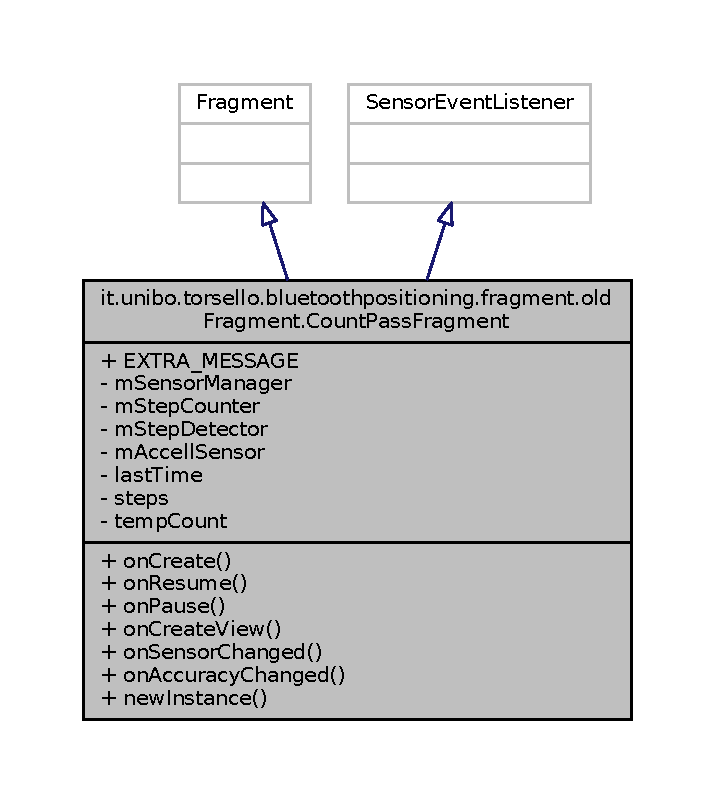
\includegraphics[width=343pt]{classit_1_1unibo_1_1torsello_1_1bluetoothpositioning_1_1fragment_1_1oldFragment_1_1CountPassFragment__inherit__graph}
\end{center}
\end{figure}


Diagramma di collaborazione per it.\+unibo.\+torsello.\+bluetoothpositioning.\+fragment.\+old\+Fragment.\+Count\+Pass\+Fragment\+:
\nopagebreak
\begin{figure}[H]
\begin{center}
\leavevmode
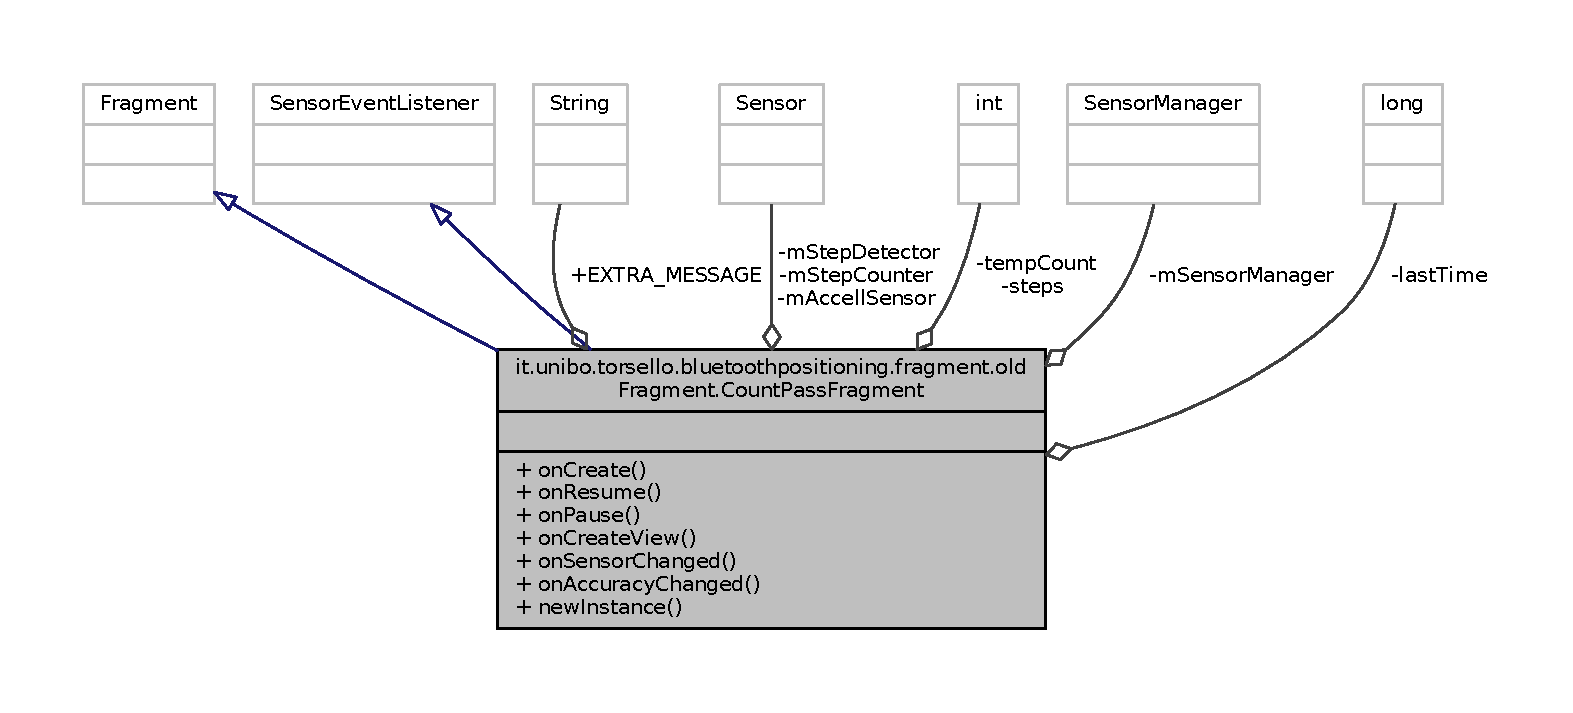
\includegraphics[width=350pt]{classit_1_1unibo_1_1torsello_1_1bluetoothpositioning_1_1fragment_1_1oldFragment_1_1CountPassFragment__coll__graph}
\end{center}
\end{figure}
\subsubsection*{Membri pubblici}
\begin{DoxyCompactItemize}
\item 
void \hyperlink{classit_1_1unibo_1_1torsello_1_1bluetoothpositioning_1_1fragment_1_1oldFragment_1_1CountPassFragment_a4f5121d2c3b4d4efb1b55d753c71a4c4_a4f5121d2c3b4d4efb1b55d753c71a4c4}{on\+Create} (Bundle saved\+Instance\+State)
\item 
void \hyperlink{classit_1_1unibo_1_1torsello_1_1bluetoothpositioning_1_1fragment_1_1oldFragment_1_1CountPassFragment_a369686c1b5124f946ba06148563a33fe_a369686c1b5124f946ba06148563a33fe}{on\+Resume} ()
\item 
void \hyperlink{classit_1_1unibo_1_1torsello_1_1bluetoothpositioning_1_1fragment_1_1oldFragment_1_1CountPassFragment_afae67ea2360d6a57e1e6bb3a1a8f2d83_afae67ea2360d6a57e1e6bb3a1a8f2d83}{on\+Pause} ()
\item 
View \hyperlink{classit_1_1unibo_1_1torsello_1_1bluetoothpositioning_1_1fragment_1_1oldFragment_1_1CountPassFragment_a2c7d7b72b37f42ab65321dba532d10cb_a2c7d7b72b37f42ab65321dba532d10cb}{on\+Create\+View} (Layout\+Inflater inflater, View\+Group container, Bundle saved\+Instance\+State)
\item 
void \hyperlink{classit_1_1unibo_1_1torsello_1_1bluetoothpositioning_1_1fragment_1_1oldFragment_1_1CountPassFragment_a278dd4ec68b222361517aed048efea68_a278dd4ec68b222361517aed048efea68}{on\+Sensor\+Changed} (Sensor\+Event event)
\item 
void \hyperlink{classit_1_1unibo_1_1torsello_1_1bluetoothpositioning_1_1fragment_1_1oldFragment_1_1CountPassFragment_a6e43aa183aa10d77db7129375cc9d487_a6e43aa183aa10d77db7129375cc9d487}{on\+Accuracy\+Changed} (Sensor sensor, int accuracy)
\end{DoxyCompactItemize}
\subsubsection*{Membri pubblici statici}
\begin{DoxyCompactItemize}
\item 
static \hyperlink{classit_1_1unibo_1_1torsello_1_1bluetoothpositioning_1_1fragment_1_1oldFragment_1_1CountPassFragment}{Count\+Pass\+Fragment} \hyperlink{classit_1_1unibo_1_1torsello_1_1bluetoothpositioning_1_1fragment_1_1oldFragment_1_1CountPassFragment_a0a03d5af96a619bfbc6e296447a325e9_a0a03d5af96a619bfbc6e296447a325e9}{new\+Instance} (String message)
\end{DoxyCompactItemize}
\subsubsection*{Attributi pubblici statici}
\begin{DoxyCompactItemize}
\item 
static final String \hyperlink{classit_1_1unibo_1_1torsello_1_1bluetoothpositioning_1_1fragment_1_1oldFragment_1_1CountPassFragment_a5729b3e7bd788b7d1b586938ced085d8_a5729b3e7bd788b7d1b586938ced085d8}{E\+X\+T\+R\+A\+\_\+\+M\+E\+S\+S\+A\+GE} = \char`\"{}E\+X\+T\+R\+A\+\_\+\+M\+E\+S\+S\+A\+GE\char`\"{}
\end{DoxyCompactItemize}
\subsubsection*{Attributi privati}
\begin{DoxyCompactItemize}
\item 
Sensor\+Manager \hyperlink{classit_1_1unibo_1_1torsello_1_1bluetoothpositioning_1_1fragment_1_1oldFragment_1_1CountPassFragment_a24e4aafb3d377f25aa09024e196d4d8d_a24e4aafb3d377f25aa09024e196d4d8d}{m\+Sensor\+Manager}
\item 
Sensor \hyperlink{classit_1_1unibo_1_1torsello_1_1bluetoothpositioning_1_1fragment_1_1oldFragment_1_1CountPassFragment_afd05ecb723e92fbb3d27bf4978e256bc_afd05ecb723e92fbb3d27bf4978e256bc}{m\+Step\+Counter}
\item 
Sensor \hyperlink{classit_1_1unibo_1_1torsello_1_1bluetoothpositioning_1_1fragment_1_1oldFragment_1_1CountPassFragment_a83913867971bc949eeff6aa7780cbff2_a83913867971bc949eeff6aa7780cbff2}{m\+Step\+Detector}
\item 
Sensor \hyperlink{classit_1_1unibo_1_1torsello_1_1bluetoothpositioning_1_1fragment_1_1oldFragment_1_1CountPassFragment_a5ceea3320c4813a465731b5f8cd36ce2_a5ceea3320c4813a465731b5f8cd36ce2}{m\+Accell\+Sensor}
\item 
long \hyperlink{classit_1_1unibo_1_1torsello_1_1bluetoothpositioning_1_1fragment_1_1oldFragment_1_1CountPassFragment_a0b2cb1d00e5c90bf8edc6997aee6fb2e_a0b2cb1d00e5c90bf8edc6997aee6fb2e}{last\+Time} = 0L
\item 
int \hyperlink{classit_1_1unibo_1_1torsello_1_1bluetoothpositioning_1_1fragment_1_1oldFragment_1_1CountPassFragment_a61757f08791ab239bac96f4a086b8d44_a61757f08791ab239bac96f4a086b8d44}{steps} = 0
\item 
int \hyperlink{classit_1_1unibo_1_1torsello_1_1bluetoothpositioning_1_1fragment_1_1oldFragment_1_1CountPassFragment_a2587f4727a7290c2252e88ebfd10a56e_a2587f4727a7290c2252e88ebfd10a56e}{temp\+Count}
\end{DoxyCompactItemize}


\subsubsection{Descrizione dettagliata}
Created by Federico Torsello. \href{mailto:federico.torsello@studio.unibo.it}{\tt federico.\+torsello@studio.\+unibo.\+it} 

\subsubsection{Documentazione delle funzioni membro}
\hypertarget{classit_1_1unibo_1_1torsello_1_1bluetoothpositioning_1_1fragment_1_1oldFragment_1_1CountPassFragment_a0a03d5af96a619bfbc6e296447a325e9_a0a03d5af96a619bfbc6e296447a325e9}{}\label{classit_1_1unibo_1_1torsello_1_1bluetoothpositioning_1_1fragment_1_1oldFragment_1_1CountPassFragment_a0a03d5af96a619bfbc6e296447a325e9_a0a03d5af96a619bfbc6e296447a325e9} 
\index{it\+::unibo\+::torsello\+::bluetoothpositioning\+::fragment\+::old\+Fragment\+::\+Count\+Pass\+Fragment@{it\+::unibo\+::torsello\+::bluetoothpositioning\+::fragment\+::old\+Fragment\+::\+Count\+Pass\+Fragment}!new\+Instance@{new\+Instance}}
\index{new\+Instance@{new\+Instance}!it\+::unibo\+::torsello\+::bluetoothpositioning\+::fragment\+::old\+Fragment\+::\+Count\+Pass\+Fragment@{it\+::unibo\+::torsello\+::bluetoothpositioning\+::fragment\+::old\+Fragment\+::\+Count\+Pass\+Fragment}}
\paragraph{\texorpdfstring{new\+Instance()}{newInstance()}}
{\footnotesize\ttfamily static \hyperlink{classit_1_1unibo_1_1torsello_1_1bluetoothpositioning_1_1fragment_1_1oldFragment_1_1CountPassFragment}{Count\+Pass\+Fragment} it.\+unibo.\+torsello.\+bluetoothpositioning.\+fragment.\+old\+Fragment.\+Count\+Pass\+Fragment.\+new\+Instance (\begin{DoxyParamCaption}\item[{String}]{message }\end{DoxyParamCaption})\hspace{0.3cm}{\ttfamily [static]}}


\begin{DoxyCode}
34                                                                 \{
35         CountPassFragment fragment = \textcolor{keyword}{new} CountPassFragment();
36         Bundle args = \textcolor{keyword}{new} Bundle();
37         args.putString(\hyperlink{classit_1_1unibo_1_1torsello_1_1bluetoothpositioning_1_1fragment_1_1oldFragment_1_1CountPassFragment_a5729b3e7bd788b7d1b586938ced085d8_a5729b3e7bd788b7d1b586938ced085d8}{EXTRA\_MESSAGE}, message);
38         fragment.setArguments(args);
39         \textcolor{keywordflow}{return} fragment;
40     \}
\end{DoxyCode}
\hypertarget{classit_1_1unibo_1_1torsello_1_1bluetoothpositioning_1_1fragment_1_1oldFragment_1_1CountPassFragment_a6e43aa183aa10d77db7129375cc9d487_a6e43aa183aa10d77db7129375cc9d487}{}\label{classit_1_1unibo_1_1torsello_1_1bluetoothpositioning_1_1fragment_1_1oldFragment_1_1CountPassFragment_a6e43aa183aa10d77db7129375cc9d487_a6e43aa183aa10d77db7129375cc9d487} 
\index{it\+::unibo\+::torsello\+::bluetoothpositioning\+::fragment\+::old\+Fragment\+::\+Count\+Pass\+Fragment@{it\+::unibo\+::torsello\+::bluetoothpositioning\+::fragment\+::old\+Fragment\+::\+Count\+Pass\+Fragment}!on\+Accuracy\+Changed@{on\+Accuracy\+Changed}}
\index{on\+Accuracy\+Changed@{on\+Accuracy\+Changed}!it\+::unibo\+::torsello\+::bluetoothpositioning\+::fragment\+::old\+Fragment\+::\+Count\+Pass\+Fragment@{it\+::unibo\+::torsello\+::bluetoothpositioning\+::fragment\+::old\+Fragment\+::\+Count\+Pass\+Fragment}}
\paragraph{\texorpdfstring{on\+Accuracy\+Changed()}{onAccuracyChanged()}}
{\footnotesize\ttfamily void it.\+unibo.\+torsello.\+bluetoothpositioning.\+fragment.\+old\+Fragment.\+Count\+Pass\+Fragment.\+on\+Accuracy\+Changed (\begin{DoxyParamCaption}\item[{Sensor}]{sensor,  }\item[{int}]{accuracy }\end{DoxyParamCaption})}


\begin{DoxyCode}
145                                                                \{
146     \}
\end{DoxyCode}
\hypertarget{classit_1_1unibo_1_1torsello_1_1bluetoothpositioning_1_1fragment_1_1oldFragment_1_1CountPassFragment_a4f5121d2c3b4d4efb1b55d753c71a4c4_a4f5121d2c3b4d4efb1b55d753c71a4c4}{}\label{classit_1_1unibo_1_1torsello_1_1bluetoothpositioning_1_1fragment_1_1oldFragment_1_1CountPassFragment_a4f5121d2c3b4d4efb1b55d753c71a4c4_a4f5121d2c3b4d4efb1b55d753c71a4c4} 
\index{it\+::unibo\+::torsello\+::bluetoothpositioning\+::fragment\+::old\+Fragment\+::\+Count\+Pass\+Fragment@{it\+::unibo\+::torsello\+::bluetoothpositioning\+::fragment\+::old\+Fragment\+::\+Count\+Pass\+Fragment}!on\+Create@{on\+Create}}
\index{on\+Create@{on\+Create}!it\+::unibo\+::torsello\+::bluetoothpositioning\+::fragment\+::old\+Fragment\+::\+Count\+Pass\+Fragment@{it\+::unibo\+::torsello\+::bluetoothpositioning\+::fragment\+::old\+Fragment\+::\+Count\+Pass\+Fragment}}
\paragraph{\texorpdfstring{on\+Create()}{onCreate()}}
{\footnotesize\ttfamily void it.\+unibo.\+torsello.\+bluetoothpositioning.\+fragment.\+old\+Fragment.\+Count\+Pass\+Fragment.\+on\+Create (\begin{DoxyParamCaption}\item[{Bundle}]{saved\+Instance\+State }\end{DoxyParamCaption})}


\begin{DoxyCode}
43                                                     \{
44         super.onCreate(savedInstanceState);
45 
46         \hyperlink{classit_1_1unibo_1_1torsello_1_1bluetoothpositioning_1_1fragment_1_1oldFragment_1_1CountPassFragment_a24e4aafb3d377f25aa09024e196d4d8d_a24e4aafb3d377f25aa09024e196d4d8d}{mSensorManager} = (SensorManager) getActivity().getSystemService(Context.
      SENSOR\_SERVICE);
47 
48         \textcolor{keywordflow}{if} (Build.VERSION.SDK\_INT >= Build.VERSION\_CODES.KITKAT) \{
49             \hyperlink{classit_1_1unibo_1_1torsello_1_1bluetoothpositioning_1_1fragment_1_1oldFragment_1_1CountPassFragment_afd05ecb723e92fbb3d27bf4978e256bc_afd05ecb723e92fbb3d27bf4978e256bc}{mStepCounter} = \hyperlink{classit_1_1unibo_1_1torsello_1_1bluetoothpositioning_1_1fragment_1_1oldFragment_1_1CountPassFragment_a24e4aafb3d377f25aa09024e196d4d8d_a24e4aafb3d377f25aa09024e196d4d8d}{mSensorManager}.getDefaultSensor(Sensor.
      TYPE\_STEP\_COUNTER);
50             \hyperlink{classit_1_1unibo_1_1torsello_1_1bluetoothpositioning_1_1fragment_1_1oldFragment_1_1CountPassFragment_a83913867971bc949eeff6aa7780cbff2_a83913867971bc949eeff6aa7780cbff2}{mStepDetector} = \hyperlink{classit_1_1unibo_1_1torsello_1_1bluetoothpositioning_1_1fragment_1_1oldFragment_1_1CountPassFragment_a24e4aafb3d377f25aa09024e196d4d8d_a24e4aafb3d377f25aa09024e196d4d8d}{mSensorManager}.getDefaultSensor(Sensor.
      TYPE\_STEP\_DETECTOR);
51         \}
52 
53         \textcolor{keywordflow}{if} (\hyperlink{classit_1_1unibo_1_1torsello_1_1bluetoothpositioning_1_1fragment_1_1oldFragment_1_1CountPassFragment_afd05ecb723e92fbb3d27bf4978e256bc_afd05ecb723e92fbb3d27bf4978e256bc}{mStepCounter} == null && \hyperlink{classit_1_1unibo_1_1torsello_1_1bluetoothpositioning_1_1fragment_1_1oldFragment_1_1CountPassFragment_a83913867971bc949eeff6aa7780cbff2_a83913867971bc949eeff6aa7780cbff2}{mStepDetector} == null) \{
54             \hyperlink{classit_1_1unibo_1_1torsello_1_1bluetoothpositioning_1_1fragment_1_1oldFragment_1_1CountPassFragment_a5ceea3320c4813a465731b5f8cd36ce2_a5ceea3320c4813a465731b5f8cd36ce2}{mAccellSensor} = \hyperlink{classit_1_1unibo_1_1torsello_1_1bluetoothpositioning_1_1fragment_1_1oldFragment_1_1CountPassFragment_a24e4aafb3d377f25aa09024e196d4d8d_a24e4aafb3d377f25aa09024e196d4d8d}{mSensorManager}.getDefaultSensor(Sensor.
      TYPE\_ACCELEROMETER);
55         \}
56 
57     \}
\end{DoxyCode}
\hypertarget{classit_1_1unibo_1_1torsello_1_1bluetoothpositioning_1_1fragment_1_1oldFragment_1_1CountPassFragment_a2c7d7b72b37f42ab65321dba532d10cb_a2c7d7b72b37f42ab65321dba532d10cb}{}\label{classit_1_1unibo_1_1torsello_1_1bluetoothpositioning_1_1fragment_1_1oldFragment_1_1CountPassFragment_a2c7d7b72b37f42ab65321dba532d10cb_a2c7d7b72b37f42ab65321dba532d10cb} 
\index{it\+::unibo\+::torsello\+::bluetoothpositioning\+::fragment\+::old\+Fragment\+::\+Count\+Pass\+Fragment@{it\+::unibo\+::torsello\+::bluetoothpositioning\+::fragment\+::old\+Fragment\+::\+Count\+Pass\+Fragment}!on\+Create\+View@{on\+Create\+View}}
\index{on\+Create\+View@{on\+Create\+View}!it\+::unibo\+::torsello\+::bluetoothpositioning\+::fragment\+::old\+Fragment\+::\+Count\+Pass\+Fragment@{it\+::unibo\+::torsello\+::bluetoothpositioning\+::fragment\+::old\+Fragment\+::\+Count\+Pass\+Fragment}}
\paragraph{\texorpdfstring{on\+Create\+View()}{onCreateView()}}
{\footnotesize\ttfamily View it.\+unibo.\+torsello.\+bluetoothpositioning.\+fragment.\+old\+Fragment.\+Count\+Pass\+Fragment.\+on\+Create\+View (\begin{DoxyParamCaption}\item[{Layout\+Inflater}]{inflater,  }\item[{View\+Group}]{container,  }\item[{Bundle}]{saved\+Instance\+State }\end{DoxyParamCaption})}


\begin{DoxyCode}
97                                                                                                       \{
98         \textcolor{keywordflow}{return} inflater.inflate(R.layout.fragment\_count\_pass, container, \textcolor{keyword}{false});
99     \}
\end{DoxyCode}
\hypertarget{classit_1_1unibo_1_1torsello_1_1bluetoothpositioning_1_1fragment_1_1oldFragment_1_1CountPassFragment_afae67ea2360d6a57e1e6bb3a1a8f2d83_afae67ea2360d6a57e1e6bb3a1a8f2d83}{}\label{classit_1_1unibo_1_1torsello_1_1bluetoothpositioning_1_1fragment_1_1oldFragment_1_1CountPassFragment_afae67ea2360d6a57e1e6bb3a1a8f2d83_afae67ea2360d6a57e1e6bb3a1a8f2d83} 
\index{it\+::unibo\+::torsello\+::bluetoothpositioning\+::fragment\+::old\+Fragment\+::\+Count\+Pass\+Fragment@{it\+::unibo\+::torsello\+::bluetoothpositioning\+::fragment\+::old\+Fragment\+::\+Count\+Pass\+Fragment}!on\+Pause@{on\+Pause}}
\index{on\+Pause@{on\+Pause}!it\+::unibo\+::torsello\+::bluetoothpositioning\+::fragment\+::old\+Fragment\+::\+Count\+Pass\+Fragment@{it\+::unibo\+::torsello\+::bluetoothpositioning\+::fragment\+::old\+Fragment\+::\+Count\+Pass\+Fragment}}
\paragraph{\texorpdfstring{on\+Pause()}{onPause()}}
{\footnotesize\ttfamily void it.\+unibo.\+torsello.\+bluetoothpositioning.\+fragment.\+old\+Fragment.\+Count\+Pass\+Fragment.\+on\+Pause (\begin{DoxyParamCaption}{ }\end{DoxyParamCaption})}


\begin{DoxyCode}
86                           \{
87         super.onPause();
88         \textcolor{keywordflow}{if} (\hyperlink{classit_1_1unibo_1_1torsello_1_1bluetoothpositioning_1_1fragment_1_1oldFragment_1_1CountPassFragment_afd05ecb723e92fbb3d27bf4978e256bc_afd05ecb723e92fbb3d27bf4978e256bc}{mStepCounter} != null && \hyperlink{classit_1_1unibo_1_1torsello_1_1bluetoothpositioning_1_1fragment_1_1oldFragment_1_1CountPassFragment_a83913867971bc949eeff6aa7780cbff2_a83913867971bc949eeff6aa7780cbff2}{mStepDetector} != null) \{
89             \hyperlink{classit_1_1unibo_1_1torsello_1_1bluetoothpositioning_1_1fragment_1_1oldFragment_1_1CountPassFragment_a24e4aafb3d377f25aa09024e196d4d8d_a24e4aafb3d377f25aa09024e196d4d8d}{mSensorManager}.unregisterListener(\textcolor{keyword}{this}, \hyperlink{classit_1_1unibo_1_1torsello_1_1bluetoothpositioning_1_1fragment_1_1oldFragment_1_1CountPassFragment_afd05ecb723e92fbb3d27bf4978e256bc_afd05ecb723e92fbb3d27bf4978e256bc}{mStepCounter});
90             \hyperlink{classit_1_1unibo_1_1torsello_1_1bluetoothpositioning_1_1fragment_1_1oldFragment_1_1CountPassFragment_a24e4aafb3d377f25aa09024e196d4d8d_a24e4aafb3d377f25aa09024e196d4d8d}{mSensorManager}.unregisterListener(\textcolor{keyword}{this}, \hyperlink{classit_1_1unibo_1_1torsello_1_1bluetoothpositioning_1_1fragment_1_1oldFragment_1_1CountPassFragment_a83913867971bc949eeff6aa7780cbff2_a83913867971bc949eeff6aa7780cbff2}{mStepDetector});
91         \} \textcolor{keywordflow}{else} \{
92             \hyperlink{classit_1_1unibo_1_1torsello_1_1bluetoothpositioning_1_1fragment_1_1oldFragment_1_1CountPassFragment_a24e4aafb3d377f25aa09024e196d4d8d_a24e4aafb3d377f25aa09024e196d4d8d}{mSensorManager}.unregisterListener(\textcolor{keyword}{this}, \hyperlink{classit_1_1unibo_1_1torsello_1_1bluetoothpositioning_1_1fragment_1_1oldFragment_1_1CountPassFragment_a5ceea3320c4813a465731b5f8cd36ce2_a5ceea3320c4813a465731b5f8cd36ce2}{mAccellSensor});
93         \}
94     \}
\end{DoxyCode}
\hypertarget{classit_1_1unibo_1_1torsello_1_1bluetoothpositioning_1_1fragment_1_1oldFragment_1_1CountPassFragment_a369686c1b5124f946ba06148563a33fe_a369686c1b5124f946ba06148563a33fe}{}\label{classit_1_1unibo_1_1torsello_1_1bluetoothpositioning_1_1fragment_1_1oldFragment_1_1CountPassFragment_a369686c1b5124f946ba06148563a33fe_a369686c1b5124f946ba06148563a33fe} 
\index{it\+::unibo\+::torsello\+::bluetoothpositioning\+::fragment\+::old\+Fragment\+::\+Count\+Pass\+Fragment@{it\+::unibo\+::torsello\+::bluetoothpositioning\+::fragment\+::old\+Fragment\+::\+Count\+Pass\+Fragment}!on\+Resume@{on\+Resume}}
\index{on\+Resume@{on\+Resume}!it\+::unibo\+::torsello\+::bluetoothpositioning\+::fragment\+::old\+Fragment\+::\+Count\+Pass\+Fragment@{it\+::unibo\+::torsello\+::bluetoothpositioning\+::fragment\+::old\+Fragment\+::\+Count\+Pass\+Fragment}}
\paragraph{\texorpdfstring{on\+Resume()}{onResume()}}
{\footnotesize\ttfamily void it.\+unibo.\+torsello.\+bluetoothpositioning.\+fragment.\+old\+Fragment.\+Count\+Pass\+Fragment.\+on\+Resume (\begin{DoxyParamCaption}{ }\end{DoxyParamCaption})}


\begin{DoxyCode}
60                            \{
61         super.onResume();
62         \textcolor{keywordflow}{if} (Build.VERSION.SDK\_INT >= Build.VERSION\_CODES.KITKAT) \{
63             \textcolor{keywordflow}{if} (\hyperlink{classit_1_1unibo_1_1torsello_1_1bluetoothpositioning_1_1fragment_1_1oldFragment_1_1CountPassFragment_afd05ecb723e92fbb3d27bf4978e256bc_afd05ecb723e92fbb3d27bf4978e256bc}{mStepCounter} != null) \{
64                 \hyperlink{classit_1_1unibo_1_1torsello_1_1bluetoothpositioning_1_1fragment_1_1oldFragment_1_1CountPassFragment_a24e4aafb3d377f25aa09024e196d4d8d_a24e4aafb3d377f25aa09024e196d4d8d}{mSensorManager}.registerListener(\textcolor{keyword}{this}, \hyperlink{classit_1_1unibo_1_1torsello_1_1bluetoothpositioning_1_1fragment_1_1oldFragment_1_1CountPassFragment_afd05ecb723e92fbb3d27bf4978e256bc_afd05ecb723e92fbb3d27bf4978e256bc}{mStepCounter}, SensorManager
      .SENSOR\_DELAY\_FASTEST,
65                         SensorManager.SENSOR\_STATUS\_ACCURACY\_HIGH);
66 \textcolor{comment}{//                mSensorManager.registerListener(this, mStepCounter, SensorManager.SENSOR\_DELAY\_FASTEST);}
67             \}
68 
69             \textcolor{keywordflow}{if} (\hyperlink{classit_1_1unibo_1_1torsello_1_1bluetoothpositioning_1_1fragment_1_1oldFragment_1_1CountPassFragment_a83913867971bc949eeff6aa7780cbff2_a83913867971bc949eeff6aa7780cbff2}{mStepDetector} != null) \{
70                 \hyperlink{classit_1_1unibo_1_1torsello_1_1bluetoothpositioning_1_1fragment_1_1oldFragment_1_1CountPassFragment_a24e4aafb3d377f25aa09024e196d4d8d_a24e4aafb3d377f25aa09024e196d4d8d}{mSensorManager}.registerListener(\textcolor{keyword}{this}, 
      \hyperlink{classit_1_1unibo_1_1torsello_1_1bluetoothpositioning_1_1fragment_1_1oldFragment_1_1CountPassFragment_a83913867971bc949eeff6aa7780cbff2_a83913867971bc949eeff6aa7780cbff2}{mStepDetector}, SensorManager.SENSOR\_DELAY\_FASTEST,
71                         SensorManager.SENSOR\_STATUS\_ACCURACY\_HIGH);
72 \textcolor{comment}{//                mSensorManager.registerListener(this, mStepDetector, SensorManager.SENSOR\_DELAY\_FASTEST);}
73             \}
74         \}
75 
76         \textcolor{keywordflow}{if} (\hyperlink{classit_1_1unibo_1_1torsello_1_1bluetoothpositioning_1_1fragment_1_1oldFragment_1_1CountPassFragment_afd05ecb723e92fbb3d27bf4978e256bc_afd05ecb723e92fbb3d27bf4978e256bc}{mStepCounter} == null && \hyperlink{classit_1_1unibo_1_1torsello_1_1bluetoothpositioning_1_1fragment_1_1oldFragment_1_1CountPassFragment_a83913867971bc949eeff6aa7780cbff2_a83913867971bc949eeff6aa7780cbff2}{mStepDetector} == null) \{
77             \textcolor{keywordflow}{if} (Build.VERSION.SDK\_INT >= Build.VERSION\_CODES.KITKAT) \{
78                 \hyperlink{classit_1_1unibo_1_1torsello_1_1bluetoothpositioning_1_1fragment_1_1oldFragment_1_1CountPassFragment_a24e4aafb3d377f25aa09024e196d4d8d_a24e4aafb3d377f25aa09024e196d4d8d}{mSensorManager}.registerListener(\textcolor{keyword}{this}, 
      \hyperlink{classit_1_1unibo_1_1torsello_1_1bluetoothpositioning_1_1fragment_1_1oldFragment_1_1CountPassFragment_a5ceea3320c4813a465731b5f8cd36ce2_a5ceea3320c4813a465731b5f8cd36ce2}{mAccellSensor}, SensorManager.SENSOR\_DELAY\_FASTEST,
79                         SensorManager.SENSOR\_STATUS\_ACCURACY\_HIGH);
80             \} \textcolor{keywordflow}{else} \{
81                 \hyperlink{classit_1_1unibo_1_1torsello_1_1bluetoothpositioning_1_1fragment_1_1oldFragment_1_1CountPassFragment_a24e4aafb3d377f25aa09024e196d4d8d_a24e4aafb3d377f25aa09024e196d4d8d}{mSensorManager}.registerListener(\textcolor{keyword}{this}, 
      \hyperlink{classit_1_1unibo_1_1torsello_1_1bluetoothpositioning_1_1fragment_1_1oldFragment_1_1CountPassFragment_a5ceea3320c4813a465731b5f8cd36ce2_a5ceea3320c4813a465731b5f8cd36ce2}{mAccellSensor}, SensorManager.SENSOR\_DELAY\_FASTEST);
82             \}
83         \}
84     \}
\end{DoxyCode}
\hypertarget{classit_1_1unibo_1_1torsello_1_1bluetoothpositioning_1_1fragment_1_1oldFragment_1_1CountPassFragment_a278dd4ec68b222361517aed048efea68_a278dd4ec68b222361517aed048efea68}{}\label{classit_1_1unibo_1_1torsello_1_1bluetoothpositioning_1_1fragment_1_1oldFragment_1_1CountPassFragment_a278dd4ec68b222361517aed048efea68_a278dd4ec68b222361517aed048efea68} 
\index{it\+::unibo\+::torsello\+::bluetoothpositioning\+::fragment\+::old\+Fragment\+::\+Count\+Pass\+Fragment@{it\+::unibo\+::torsello\+::bluetoothpositioning\+::fragment\+::old\+Fragment\+::\+Count\+Pass\+Fragment}!on\+Sensor\+Changed@{on\+Sensor\+Changed}}
\index{on\+Sensor\+Changed@{on\+Sensor\+Changed}!it\+::unibo\+::torsello\+::bluetoothpositioning\+::fragment\+::old\+Fragment\+::\+Count\+Pass\+Fragment@{it\+::unibo\+::torsello\+::bluetoothpositioning\+::fragment\+::old\+Fragment\+::\+Count\+Pass\+Fragment}}
\paragraph{\texorpdfstring{on\+Sensor\+Changed()}{onSensorChanged()}}
{\footnotesize\ttfamily void it.\+unibo.\+torsello.\+bluetoothpositioning.\+fragment.\+old\+Fragment.\+Count\+Pass\+Fragment.\+on\+Sensor\+Changed (\begin{DoxyParamCaption}\item[{Sensor\+Event}]{event }\end{DoxyParamCaption})}


\begin{DoxyCode}
102                                                    \{
103 \textcolor{comment}{//        if (event.sensor == mStepCounter) \{}
104 \textcolor{comment}{//            stepCounter = event.values;}
105 \textcolor{comment}{//            Log.d("stepCount" , String.valueOf(stepCounter[0]));}
106 \textcolor{comment}{//        \} else if (event.sensor == mStepDetector) \{}
107 \textcolor{comment}{//            stepDetector = event.values;}
108 \textcolor{comment}{//            Log.d("stepDetector" , String.valueOf(stepDetector[0]));}
109 \textcolor{comment}{//        \}}
110 
111         \textcolor{keywordflow}{switch} (event.sensor.getType()) \{
112             \textcolor{keywordflow}{case} Sensor.TYPE\_STEP\_DETECTOR:
113                 Log.d(\textcolor{stringliteral}{"stepCount"}, String.valueOf(event.values[0]));
114                 \textcolor{keywordflow}{break};
115             \textcolor{keywordflow}{case} Sensor.TYPE\_STEP\_COUNTER:
116                 Log.d(\textcolor{stringliteral}{"stepDetector"}, String.valueOf(event.values[0]));
117                 \textcolor{keywordflow}{break};
118             \textcolor{keywordflow}{case} Sensor.TYPE\_ACCELEROMETER: \{
119                 \textcolor{keywordtype}{float} x = \textcolor{keyword}{event}.values[0];
120                 \textcolor{keywordtype}{float} y = \textcolor{keyword}{event}.values[1];
121                 \textcolor{keywordtype}{float} z = \textcolor{keyword}{event}.values[2];
122 
123                 \textcolor{keywordtype}{float} accelationSquareRoot = Math.abs((x * x + y * y + z * z)
124                         / (SensorManager.GRAVITY\_EARTH * SensorManager.GRAVITY\_EARTH)) - 1.0f;
125                 \textcolor{keywordtype}{long} actualTime = System.currentTimeMillis();
126 
127                 \textcolor{keywordflow}{if} (actualTime - \hyperlink{classit_1_1unibo_1_1torsello_1_1bluetoothpositioning_1_1fragment_1_1oldFragment_1_1CountPassFragment_a0b2cb1d00e5c90bf8edc6997aee6fb2e_a0b2cb1d00e5c90bf8edc6997aee6fb2e}{lastTime} > 300) \{
128                     \textcolor{keywordflow}{if} (accelationSquareRoot < -0.45f) \{
129                         \hyperlink{classit_1_1unibo_1_1torsello_1_1bluetoothpositioning_1_1fragment_1_1oldFragment_1_1CountPassFragment_a61757f08791ab239bac96f4a086b8d44_a61757f08791ab239bac96f4a086b8d44}{steps}++;
130                         \hyperlink{classit_1_1unibo_1_1torsello_1_1bluetoothpositioning_1_1fragment_1_1oldFragment_1_1CountPassFragment_a2587f4727a7290c2252e88ebfd10a56e_a2587f4727a7290c2252e88ebfd10a56e}{tempCount}++;
131                     \}
132                     \hyperlink{classit_1_1unibo_1_1torsello_1_1bluetoothpositioning_1_1fragment_1_1oldFragment_1_1CountPassFragment_a0b2cb1d00e5c90bf8edc6997aee6fb2e_a0b2cb1d00e5c90bf8edc6997aee6fb2e}{lastTime} = actualTime;
133                 \}
134 
135                 TextView textView = (TextView) getActivity().findViewById(R.id.countPassText);
136                 textView.setText(String.valueOf(\hyperlink{classit_1_1unibo_1_1torsello_1_1bluetoothpositioning_1_1fragment_1_1oldFragment_1_1CountPassFragment_a61757f08791ab239bac96f4a086b8d44_a61757f08791ab239bac96f4a086b8d44}{steps}));
137             \}
138             \textcolor{keywordflow}{break};
139         \}
140 
141 
142     \}
\end{DoxyCode}


\subsubsection{Documentazione dei membri dato}
\hypertarget{classit_1_1unibo_1_1torsello_1_1bluetoothpositioning_1_1fragment_1_1oldFragment_1_1CountPassFragment_a5729b3e7bd788b7d1b586938ced085d8_a5729b3e7bd788b7d1b586938ced085d8}{}\label{classit_1_1unibo_1_1torsello_1_1bluetoothpositioning_1_1fragment_1_1oldFragment_1_1CountPassFragment_a5729b3e7bd788b7d1b586938ced085d8_a5729b3e7bd788b7d1b586938ced085d8} 
\index{it\+::unibo\+::torsello\+::bluetoothpositioning\+::fragment\+::old\+Fragment\+::\+Count\+Pass\+Fragment@{it\+::unibo\+::torsello\+::bluetoothpositioning\+::fragment\+::old\+Fragment\+::\+Count\+Pass\+Fragment}!E\+X\+T\+R\+A\+\_\+\+M\+E\+S\+S\+A\+GE@{E\+X\+T\+R\+A\+\_\+\+M\+E\+S\+S\+A\+GE}}
\index{E\+X\+T\+R\+A\+\_\+\+M\+E\+S\+S\+A\+GE@{E\+X\+T\+R\+A\+\_\+\+M\+E\+S\+S\+A\+GE}!it\+::unibo\+::torsello\+::bluetoothpositioning\+::fragment\+::old\+Fragment\+::\+Count\+Pass\+Fragment@{it\+::unibo\+::torsello\+::bluetoothpositioning\+::fragment\+::old\+Fragment\+::\+Count\+Pass\+Fragment}}
\paragraph{\texorpdfstring{E\+X\+T\+R\+A\+\_\+\+M\+E\+S\+S\+A\+GE}{EXTRA\_MESSAGE}}
{\footnotesize\ttfamily final String it.\+unibo.\+torsello.\+bluetoothpositioning.\+fragment.\+old\+Fragment.\+Count\+Pass\+Fragment.\+E\+X\+T\+R\+A\+\_\+\+M\+E\+S\+S\+A\+GE = \char`\"{}E\+X\+T\+R\+A\+\_\+\+M\+E\+S\+S\+A\+GE\char`\"{}\hspace{0.3cm}{\ttfamily [static]}}

\hypertarget{classit_1_1unibo_1_1torsello_1_1bluetoothpositioning_1_1fragment_1_1oldFragment_1_1CountPassFragment_a0b2cb1d00e5c90bf8edc6997aee6fb2e_a0b2cb1d00e5c90bf8edc6997aee6fb2e}{}\label{classit_1_1unibo_1_1torsello_1_1bluetoothpositioning_1_1fragment_1_1oldFragment_1_1CountPassFragment_a0b2cb1d00e5c90bf8edc6997aee6fb2e_a0b2cb1d00e5c90bf8edc6997aee6fb2e} 
\index{it\+::unibo\+::torsello\+::bluetoothpositioning\+::fragment\+::old\+Fragment\+::\+Count\+Pass\+Fragment@{it\+::unibo\+::torsello\+::bluetoothpositioning\+::fragment\+::old\+Fragment\+::\+Count\+Pass\+Fragment}!last\+Time@{last\+Time}}
\index{last\+Time@{last\+Time}!it\+::unibo\+::torsello\+::bluetoothpositioning\+::fragment\+::old\+Fragment\+::\+Count\+Pass\+Fragment@{it\+::unibo\+::torsello\+::bluetoothpositioning\+::fragment\+::old\+Fragment\+::\+Count\+Pass\+Fragment}}
\paragraph{\texorpdfstring{last\+Time}{lastTime}}
{\footnotesize\ttfamily long it.\+unibo.\+torsello.\+bluetoothpositioning.\+fragment.\+old\+Fragment.\+Count\+Pass\+Fragment.\+last\+Time = 0L\hspace{0.3cm}{\ttfamily [private]}}

\hypertarget{classit_1_1unibo_1_1torsello_1_1bluetoothpositioning_1_1fragment_1_1oldFragment_1_1CountPassFragment_a5ceea3320c4813a465731b5f8cd36ce2_a5ceea3320c4813a465731b5f8cd36ce2}{}\label{classit_1_1unibo_1_1torsello_1_1bluetoothpositioning_1_1fragment_1_1oldFragment_1_1CountPassFragment_a5ceea3320c4813a465731b5f8cd36ce2_a5ceea3320c4813a465731b5f8cd36ce2} 
\index{it\+::unibo\+::torsello\+::bluetoothpositioning\+::fragment\+::old\+Fragment\+::\+Count\+Pass\+Fragment@{it\+::unibo\+::torsello\+::bluetoothpositioning\+::fragment\+::old\+Fragment\+::\+Count\+Pass\+Fragment}!m\+Accell\+Sensor@{m\+Accell\+Sensor}}
\index{m\+Accell\+Sensor@{m\+Accell\+Sensor}!it\+::unibo\+::torsello\+::bluetoothpositioning\+::fragment\+::old\+Fragment\+::\+Count\+Pass\+Fragment@{it\+::unibo\+::torsello\+::bluetoothpositioning\+::fragment\+::old\+Fragment\+::\+Count\+Pass\+Fragment}}
\paragraph{\texorpdfstring{m\+Accell\+Sensor}{mAccellSensor}}
{\footnotesize\ttfamily Sensor it.\+unibo.\+torsello.\+bluetoothpositioning.\+fragment.\+old\+Fragment.\+Count\+Pass\+Fragment.\+m\+Accell\+Sensor\hspace{0.3cm}{\ttfamily [private]}}

\hypertarget{classit_1_1unibo_1_1torsello_1_1bluetoothpositioning_1_1fragment_1_1oldFragment_1_1CountPassFragment_a24e4aafb3d377f25aa09024e196d4d8d_a24e4aafb3d377f25aa09024e196d4d8d}{}\label{classit_1_1unibo_1_1torsello_1_1bluetoothpositioning_1_1fragment_1_1oldFragment_1_1CountPassFragment_a24e4aafb3d377f25aa09024e196d4d8d_a24e4aafb3d377f25aa09024e196d4d8d} 
\index{it\+::unibo\+::torsello\+::bluetoothpositioning\+::fragment\+::old\+Fragment\+::\+Count\+Pass\+Fragment@{it\+::unibo\+::torsello\+::bluetoothpositioning\+::fragment\+::old\+Fragment\+::\+Count\+Pass\+Fragment}!m\+Sensor\+Manager@{m\+Sensor\+Manager}}
\index{m\+Sensor\+Manager@{m\+Sensor\+Manager}!it\+::unibo\+::torsello\+::bluetoothpositioning\+::fragment\+::old\+Fragment\+::\+Count\+Pass\+Fragment@{it\+::unibo\+::torsello\+::bluetoothpositioning\+::fragment\+::old\+Fragment\+::\+Count\+Pass\+Fragment}}
\paragraph{\texorpdfstring{m\+Sensor\+Manager}{mSensorManager}}
{\footnotesize\ttfamily Sensor\+Manager it.\+unibo.\+torsello.\+bluetoothpositioning.\+fragment.\+old\+Fragment.\+Count\+Pass\+Fragment.\+m\+Sensor\+Manager\hspace{0.3cm}{\ttfamily [private]}}

\hypertarget{classit_1_1unibo_1_1torsello_1_1bluetoothpositioning_1_1fragment_1_1oldFragment_1_1CountPassFragment_afd05ecb723e92fbb3d27bf4978e256bc_afd05ecb723e92fbb3d27bf4978e256bc}{}\label{classit_1_1unibo_1_1torsello_1_1bluetoothpositioning_1_1fragment_1_1oldFragment_1_1CountPassFragment_afd05ecb723e92fbb3d27bf4978e256bc_afd05ecb723e92fbb3d27bf4978e256bc} 
\index{it\+::unibo\+::torsello\+::bluetoothpositioning\+::fragment\+::old\+Fragment\+::\+Count\+Pass\+Fragment@{it\+::unibo\+::torsello\+::bluetoothpositioning\+::fragment\+::old\+Fragment\+::\+Count\+Pass\+Fragment}!m\+Step\+Counter@{m\+Step\+Counter}}
\index{m\+Step\+Counter@{m\+Step\+Counter}!it\+::unibo\+::torsello\+::bluetoothpositioning\+::fragment\+::old\+Fragment\+::\+Count\+Pass\+Fragment@{it\+::unibo\+::torsello\+::bluetoothpositioning\+::fragment\+::old\+Fragment\+::\+Count\+Pass\+Fragment}}
\paragraph{\texorpdfstring{m\+Step\+Counter}{mStepCounter}}
{\footnotesize\ttfamily Sensor it.\+unibo.\+torsello.\+bluetoothpositioning.\+fragment.\+old\+Fragment.\+Count\+Pass\+Fragment.\+m\+Step\+Counter\hspace{0.3cm}{\ttfamily [private]}}

\hypertarget{classit_1_1unibo_1_1torsello_1_1bluetoothpositioning_1_1fragment_1_1oldFragment_1_1CountPassFragment_a83913867971bc949eeff6aa7780cbff2_a83913867971bc949eeff6aa7780cbff2}{}\label{classit_1_1unibo_1_1torsello_1_1bluetoothpositioning_1_1fragment_1_1oldFragment_1_1CountPassFragment_a83913867971bc949eeff6aa7780cbff2_a83913867971bc949eeff6aa7780cbff2} 
\index{it\+::unibo\+::torsello\+::bluetoothpositioning\+::fragment\+::old\+Fragment\+::\+Count\+Pass\+Fragment@{it\+::unibo\+::torsello\+::bluetoothpositioning\+::fragment\+::old\+Fragment\+::\+Count\+Pass\+Fragment}!m\+Step\+Detector@{m\+Step\+Detector}}
\index{m\+Step\+Detector@{m\+Step\+Detector}!it\+::unibo\+::torsello\+::bluetoothpositioning\+::fragment\+::old\+Fragment\+::\+Count\+Pass\+Fragment@{it\+::unibo\+::torsello\+::bluetoothpositioning\+::fragment\+::old\+Fragment\+::\+Count\+Pass\+Fragment}}
\paragraph{\texorpdfstring{m\+Step\+Detector}{mStepDetector}}
{\footnotesize\ttfamily Sensor it.\+unibo.\+torsello.\+bluetoothpositioning.\+fragment.\+old\+Fragment.\+Count\+Pass\+Fragment.\+m\+Step\+Detector\hspace{0.3cm}{\ttfamily [private]}}

\hypertarget{classit_1_1unibo_1_1torsello_1_1bluetoothpositioning_1_1fragment_1_1oldFragment_1_1CountPassFragment_a61757f08791ab239bac96f4a086b8d44_a61757f08791ab239bac96f4a086b8d44}{}\label{classit_1_1unibo_1_1torsello_1_1bluetoothpositioning_1_1fragment_1_1oldFragment_1_1CountPassFragment_a61757f08791ab239bac96f4a086b8d44_a61757f08791ab239bac96f4a086b8d44} 
\index{it\+::unibo\+::torsello\+::bluetoothpositioning\+::fragment\+::old\+Fragment\+::\+Count\+Pass\+Fragment@{it\+::unibo\+::torsello\+::bluetoothpositioning\+::fragment\+::old\+Fragment\+::\+Count\+Pass\+Fragment}!steps@{steps}}
\index{steps@{steps}!it\+::unibo\+::torsello\+::bluetoothpositioning\+::fragment\+::old\+Fragment\+::\+Count\+Pass\+Fragment@{it\+::unibo\+::torsello\+::bluetoothpositioning\+::fragment\+::old\+Fragment\+::\+Count\+Pass\+Fragment}}
\paragraph{\texorpdfstring{steps}{steps}}
{\footnotesize\ttfamily int it.\+unibo.\+torsello.\+bluetoothpositioning.\+fragment.\+old\+Fragment.\+Count\+Pass\+Fragment.\+steps = 0\hspace{0.3cm}{\ttfamily [private]}}

\hypertarget{classit_1_1unibo_1_1torsello_1_1bluetoothpositioning_1_1fragment_1_1oldFragment_1_1CountPassFragment_a2587f4727a7290c2252e88ebfd10a56e_a2587f4727a7290c2252e88ebfd10a56e}{}\label{classit_1_1unibo_1_1torsello_1_1bluetoothpositioning_1_1fragment_1_1oldFragment_1_1CountPassFragment_a2587f4727a7290c2252e88ebfd10a56e_a2587f4727a7290c2252e88ebfd10a56e} 
\index{it\+::unibo\+::torsello\+::bluetoothpositioning\+::fragment\+::old\+Fragment\+::\+Count\+Pass\+Fragment@{it\+::unibo\+::torsello\+::bluetoothpositioning\+::fragment\+::old\+Fragment\+::\+Count\+Pass\+Fragment}!temp\+Count@{temp\+Count}}
\index{temp\+Count@{temp\+Count}!it\+::unibo\+::torsello\+::bluetoothpositioning\+::fragment\+::old\+Fragment\+::\+Count\+Pass\+Fragment@{it\+::unibo\+::torsello\+::bluetoothpositioning\+::fragment\+::old\+Fragment\+::\+Count\+Pass\+Fragment}}
\paragraph{\texorpdfstring{temp\+Count}{tempCount}}
{\footnotesize\ttfamily int it.\+unibo.\+torsello.\+bluetoothpositioning.\+fragment.\+old\+Fragment.\+Count\+Pass\+Fragment.\+temp\+Count\hspace{0.3cm}{\ttfamily [private]}}



La documentazione per questa classe è stata generata a partire dal seguente file\+:\begin{DoxyCompactItemize}
\item 
\hyperlink{CountPassFragment_8java}{Count\+Pass\+Fragment.\+java}\end{DoxyCompactItemize}

\hypertarget{classit_1_1unibo_1_1torsello_1_1bluetoothpositioning_1_1model_1_1Device}{}\subsection{Riferimenti per la classe it.\+unibo.\+torsello.\+bluetoothpositioning.\+model.\+Device}
\label{classit_1_1unibo_1_1torsello_1_1bluetoothpositioning_1_1model_1_1Device}\index{it.\+unibo.\+torsello.\+bluetoothpositioning.\+model.\+Device@{it.\+unibo.\+torsello.\+bluetoothpositioning.\+model.\+Device}}


Diagramma di collaborazione per it.\+unibo.\+torsello.\+bluetoothpositioning.\+model.\+Device\+:
\nopagebreak
\begin{figure}[H]
\begin{center}
\leavevmode
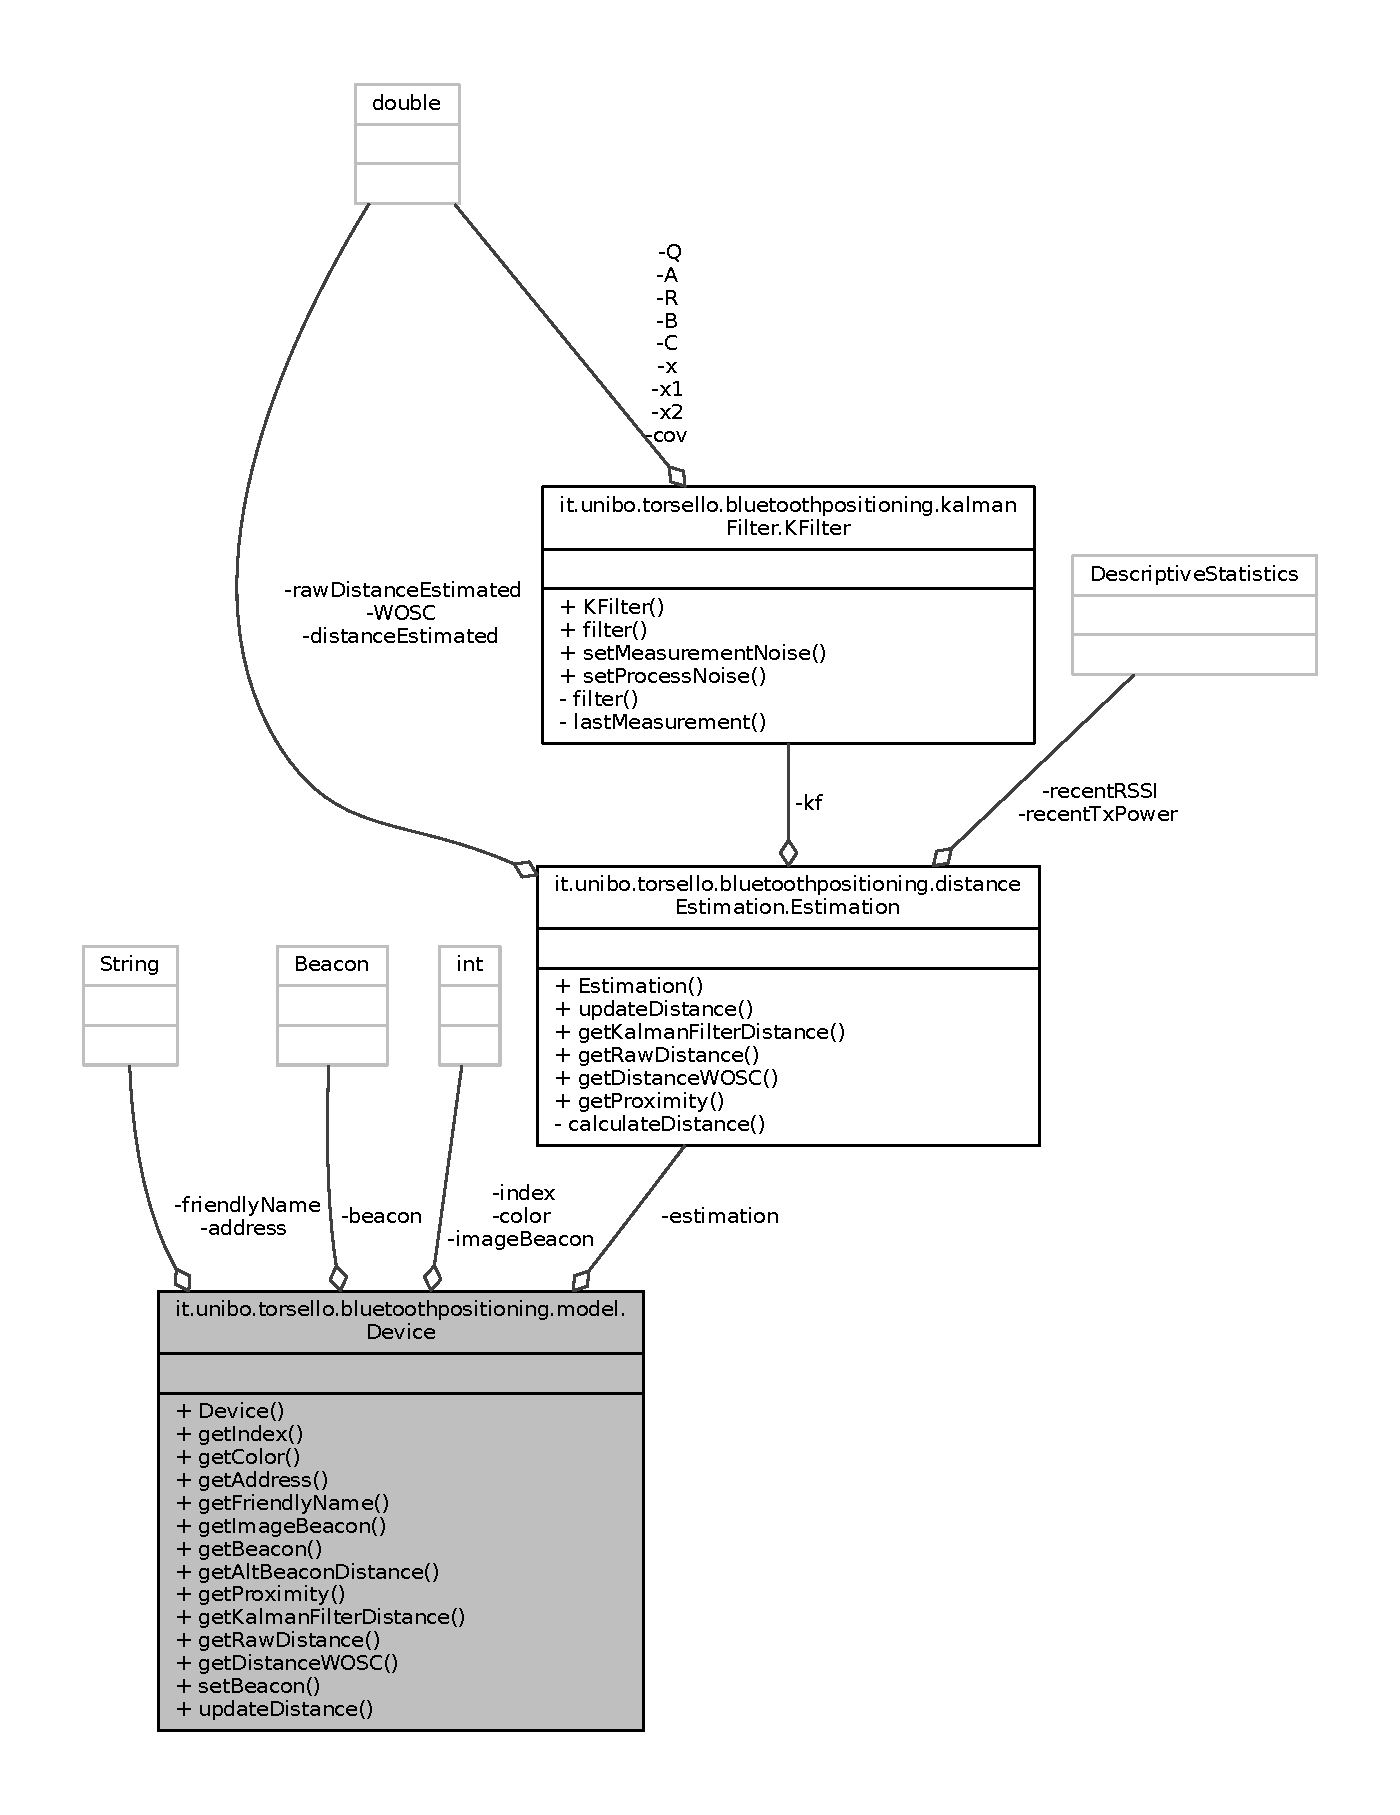
\includegraphics[width=350pt]{classit_1_1unibo_1_1torsello_1_1bluetoothpositioning_1_1model_1_1Device__coll__graph}
\end{center}
\end{figure}
\subsubsection*{Membri pubblici}
\begin{DoxyCompactItemize}
\item 
\hyperlink{classit_1_1unibo_1_1torsello_1_1bluetoothpositioning_1_1model_1_1Device_a2617f025dd33e0cae4adb3323245f865_a2617f025dd33e0cae4adb3323245f865}{Device} (int \hyperlink{classit_1_1unibo_1_1torsello_1_1bluetoothpositioning_1_1model_1_1Device_a55a01164b2388451f5e8344bfbc61ccc_a55a01164b2388451f5e8344bfbc61ccc}{index}, String \hyperlink{classit_1_1unibo_1_1torsello_1_1bluetoothpositioning_1_1model_1_1Device_a0abcf7e0df4ccc96e487c6f9b90b4e13_a0abcf7e0df4ccc96e487c6f9b90b4e13}{address}, String \hyperlink{classit_1_1unibo_1_1torsello_1_1bluetoothpositioning_1_1model_1_1Device_aa9a540b316c9de7f9b3a94f58570f6d3_aa9a540b316c9de7f9b3a94f58570f6d3}{friendly\+Name}, Integer \hyperlink{classit_1_1unibo_1_1torsello_1_1bluetoothpositioning_1_1model_1_1Device_aaba1f93e2a0f88f01262cb38a65489e6_aaba1f93e2a0f88f01262cb38a65489e6}{color}, Integer \hyperlink{classit_1_1unibo_1_1torsello_1_1bluetoothpositioning_1_1model_1_1Device_a2faee0d51162a4efebfc2db787901019_a2faee0d51162a4efebfc2db787901019}{image\+Beacon})
\item 
int \hyperlink{classit_1_1unibo_1_1torsello_1_1bluetoothpositioning_1_1model_1_1Device_a7f7e47588f721b360447d0f6ae2c4a9d_a7f7e47588f721b360447d0f6ae2c4a9d}{get\+Index} ()
\item 
Integer \hyperlink{classit_1_1unibo_1_1torsello_1_1bluetoothpositioning_1_1model_1_1Device_aad4f2885e5ed0279c7e0c6db684de5c3_aad4f2885e5ed0279c7e0c6db684de5c3}{get\+Color} ()
\item 
String \hyperlink{classit_1_1unibo_1_1torsello_1_1bluetoothpositioning_1_1model_1_1Device_ae4cd3fdda7414388cbda796f62543d5b_ae4cd3fdda7414388cbda796f62543d5b}{get\+Address} ()
\item 
String \hyperlink{classit_1_1unibo_1_1torsello_1_1bluetoothpositioning_1_1model_1_1Device_ab96e3e3bd6e9c9e27a42e619ca03ed71_ab96e3e3bd6e9c9e27a42e619ca03ed71}{get\+Friendly\+Name} ()
\item 
Integer \hyperlink{classit_1_1unibo_1_1torsello_1_1bluetoothpositioning_1_1model_1_1Device_a0fe04c6168a9a13bdf65eb0e5d407d37_a0fe04c6168a9a13bdf65eb0e5d407d37}{get\+Image\+Beacon} ()
\item 
Beacon \hyperlink{classit_1_1unibo_1_1torsello_1_1bluetoothpositioning_1_1model_1_1Device_a61b4951f3153550e8006f043eec034c2_a61b4951f3153550e8006f043eec034c2}{get\+Beacon} ()
\item 
double \hyperlink{classit_1_1unibo_1_1torsello_1_1bluetoothpositioning_1_1model_1_1Device_aa178afb829c0b5cae49af25e0e9b2117_aa178afb829c0b5cae49af25e0e9b2117}{get\+Alt\+Beacon\+Distance} ()
\item 
String \hyperlink{classit_1_1unibo_1_1torsello_1_1bluetoothpositioning_1_1model_1_1Device_a34510d139c99bc9cfba247ab6ff1b16f_a34510d139c99bc9cfba247ab6ff1b16f}{get\+Proximity} ()
\item 
double \hyperlink{classit_1_1unibo_1_1torsello_1_1bluetoothpositioning_1_1model_1_1Device_aa86454f965d50f015f1f40abe2d0d19a_aa86454f965d50f015f1f40abe2d0d19a}{get\+Kalman\+Filter\+Distance} ()
\item 
double \hyperlink{classit_1_1unibo_1_1torsello_1_1bluetoothpositioning_1_1model_1_1Device_abd5c0c1d478ac01c009959891456bbb8_abd5c0c1d478ac01c009959891456bbb8}{get\+Raw\+Distance} ()
\item 
double \hyperlink{classit_1_1unibo_1_1torsello_1_1bluetoothpositioning_1_1model_1_1Device_abcef7fbd06b5c97b412619a5b79b237c_abcef7fbd06b5c97b412619a5b79b237c}{get\+Distance\+W\+O\+SC} ()
\item 
void \hyperlink{classit_1_1unibo_1_1torsello_1_1bluetoothpositioning_1_1model_1_1Device_a7aff672e35f15a271dd93bd59e413f28_a7aff672e35f15a271dd93bd59e413f28}{set\+Beacon} (Beacon \hyperlink{classit_1_1unibo_1_1torsello_1_1bluetoothpositioning_1_1model_1_1Device_ad5ffce680eb2eb38fc6bb8aee234f155_ad5ffce680eb2eb38fc6bb8aee234f155}{beacon})
\item 
void \hyperlink{classit_1_1unibo_1_1torsello_1_1bluetoothpositioning_1_1model_1_1Device_af6e2efc8c50b88d07cc651db1f4bbb34_af6e2efc8c50b88d07cc651db1f4bbb34}{update\+Distance} (double process\+Noise)
\item 
boolean \hyperlink{classit_1_1unibo_1_1torsello_1_1bluetoothpositioning_1_1model_1_1Device_a7eb63440da744a389cc02d1d9a9b2421_a7eb63440da744a389cc02d1d9a9b2421}{is\+Kalman\+Filter\+Enabled} ()
\end{DoxyCompactItemize}
\subsubsection*{Attributi privati}
\begin{DoxyCompactItemize}
\item 
\hyperlink{classit_1_1unibo_1_1torsello_1_1bluetoothpositioning_1_1distanceEstimation_1_1Estimation}{Estimation} \hyperlink{classit_1_1unibo_1_1torsello_1_1bluetoothpositioning_1_1model_1_1Device_ac619c42728cd40f41a5f12fde56b4425_ac619c42728cd40f41a5f12fde56b4425}{estimation}
\item 
String \hyperlink{classit_1_1unibo_1_1torsello_1_1bluetoothpositioning_1_1model_1_1Device_a0abcf7e0df4ccc96e487c6f9b90b4e13_a0abcf7e0df4ccc96e487c6f9b90b4e13}{address}
\item 
String \hyperlink{classit_1_1unibo_1_1torsello_1_1bluetoothpositioning_1_1model_1_1Device_aa9a540b316c9de7f9b3a94f58570f6d3_aa9a540b316c9de7f9b3a94f58570f6d3}{friendly\+Name}
\item 
Beacon \hyperlink{classit_1_1unibo_1_1torsello_1_1bluetoothpositioning_1_1model_1_1Device_ad5ffce680eb2eb38fc6bb8aee234f155_ad5ffce680eb2eb38fc6bb8aee234f155}{beacon}
\item 
int \hyperlink{classit_1_1unibo_1_1torsello_1_1bluetoothpositioning_1_1model_1_1Device_a2faee0d51162a4efebfc2db787901019_a2faee0d51162a4efebfc2db787901019}{image\+Beacon}
\item 
int \hyperlink{classit_1_1unibo_1_1torsello_1_1bluetoothpositioning_1_1model_1_1Device_aaba1f93e2a0f88f01262cb38a65489e6_aaba1f93e2a0f88f01262cb38a65489e6}{color}
\item 
int \hyperlink{classit_1_1unibo_1_1torsello_1_1bluetoothpositioning_1_1model_1_1Device_a55a01164b2388451f5e8344bfbc61ccc_a55a01164b2388451f5e8344bfbc61ccc}{index}
\end{DoxyCompactItemize}


\subsubsection{Descrizione dettagliata}
Created by Federico Torsello. \href{mailto:federico.torsello@studio.unibo.it}{\tt federico.\+torsello@studio.\+unibo.\+it} 

\subsubsection{Documentazione dei costruttori e dei distruttori}
\hypertarget{classit_1_1unibo_1_1torsello_1_1bluetoothpositioning_1_1model_1_1Device_a2617f025dd33e0cae4adb3323245f865_a2617f025dd33e0cae4adb3323245f865}{}\label{classit_1_1unibo_1_1torsello_1_1bluetoothpositioning_1_1model_1_1Device_a2617f025dd33e0cae4adb3323245f865_a2617f025dd33e0cae4adb3323245f865} 
\index{it\+::unibo\+::torsello\+::bluetoothpositioning\+::model\+::\+Device@{it\+::unibo\+::torsello\+::bluetoothpositioning\+::model\+::\+Device}!Device@{Device}}
\index{Device@{Device}!it\+::unibo\+::torsello\+::bluetoothpositioning\+::model\+::\+Device@{it\+::unibo\+::torsello\+::bluetoothpositioning\+::model\+::\+Device}}
\paragraph{\texorpdfstring{Device()}{Device()}}
{\footnotesize\ttfamily it.\+unibo.\+torsello.\+bluetoothpositioning.\+model.\+Device.\+Device (\begin{DoxyParamCaption}\item[{int}]{index,  }\item[{String}]{address,  }\item[{String}]{friendly\+Name,  }\item[{Integer}]{color,  }\item[{Integer}]{image\+Beacon }\end{DoxyParamCaption})}


\begin{DoxyCode}
21                                                                                                       \{
22         this.\hyperlink{classit_1_1unibo_1_1torsello_1_1bluetoothpositioning_1_1model_1_1Device_a55a01164b2388451f5e8344bfbc61ccc_a55a01164b2388451f5e8344bfbc61ccc}{index} = \hyperlink{classit_1_1unibo_1_1torsello_1_1bluetoothpositioning_1_1model_1_1Device_a55a01164b2388451f5e8344bfbc61ccc_a55a01164b2388451f5e8344bfbc61ccc}{index};
23         this.\hyperlink{classit_1_1unibo_1_1torsello_1_1bluetoothpositioning_1_1model_1_1Device_a0abcf7e0df4ccc96e487c6f9b90b4e13_a0abcf7e0df4ccc96e487c6f9b90b4e13}{address} = \hyperlink{classit_1_1unibo_1_1torsello_1_1bluetoothpositioning_1_1model_1_1Device_a0abcf7e0df4ccc96e487c6f9b90b4e13_a0abcf7e0df4ccc96e487c6f9b90b4e13}{address};
24         this.\hyperlink{classit_1_1unibo_1_1torsello_1_1bluetoothpositioning_1_1model_1_1Device_aa9a540b316c9de7f9b3a94f58570f6d3_aa9a540b316c9de7f9b3a94f58570f6d3}{friendlyName} = \hyperlink{classit_1_1unibo_1_1torsello_1_1bluetoothpositioning_1_1model_1_1Device_aa9a540b316c9de7f9b3a94f58570f6d3_aa9a540b316c9de7f9b3a94f58570f6d3}{friendlyName};
25         this.\hyperlink{classit_1_1unibo_1_1torsello_1_1bluetoothpositioning_1_1model_1_1Device_ac619c42728cd40f41a5f12fde56b4425_ac619c42728cd40f41a5f12fde56b4425}{estimation} = \textcolor{keyword}{new} Estimation();
26         this.\hyperlink{classit_1_1unibo_1_1torsello_1_1bluetoothpositioning_1_1model_1_1Device_a2faee0d51162a4efebfc2db787901019_a2faee0d51162a4efebfc2db787901019}{imageBeacon} = \hyperlink{classit_1_1unibo_1_1torsello_1_1bluetoothpositioning_1_1model_1_1Device_a2faee0d51162a4efebfc2db787901019_a2faee0d51162a4efebfc2db787901019}{imageBeacon};
27         this.\hyperlink{classit_1_1unibo_1_1torsello_1_1bluetoothpositioning_1_1model_1_1Device_aaba1f93e2a0f88f01262cb38a65489e6_aaba1f93e2a0f88f01262cb38a65489e6}{color} = \hyperlink{classit_1_1unibo_1_1torsello_1_1bluetoothpositioning_1_1model_1_1Device_aaba1f93e2a0f88f01262cb38a65489e6_aaba1f93e2a0f88f01262cb38a65489e6}{color};
28     \}
\end{DoxyCode}


\subsubsection{Documentazione delle funzioni membro}
\hypertarget{classit_1_1unibo_1_1torsello_1_1bluetoothpositioning_1_1model_1_1Device_ae4cd3fdda7414388cbda796f62543d5b_ae4cd3fdda7414388cbda796f62543d5b}{}\label{classit_1_1unibo_1_1torsello_1_1bluetoothpositioning_1_1model_1_1Device_ae4cd3fdda7414388cbda796f62543d5b_ae4cd3fdda7414388cbda796f62543d5b} 
\index{it\+::unibo\+::torsello\+::bluetoothpositioning\+::model\+::\+Device@{it\+::unibo\+::torsello\+::bluetoothpositioning\+::model\+::\+Device}!get\+Address@{get\+Address}}
\index{get\+Address@{get\+Address}!it\+::unibo\+::torsello\+::bluetoothpositioning\+::model\+::\+Device@{it\+::unibo\+::torsello\+::bluetoothpositioning\+::model\+::\+Device}}
\paragraph{\texorpdfstring{get\+Address()}{getAddress()}}
{\footnotesize\ttfamily String it.\+unibo.\+torsello.\+bluetoothpositioning.\+model.\+Device.\+get\+Address (\begin{DoxyParamCaption}{ }\end{DoxyParamCaption})}


\begin{DoxyCode}
38                                \{
39         \textcolor{keywordflow}{return} this.\hyperlink{classit_1_1unibo_1_1torsello_1_1bluetoothpositioning_1_1model_1_1Device_a0abcf7e0df4ccc96e487c6f9b90b4e13_a0abcf7e0df4ccc96e487c6f9b90b4e13}{address};
40     \}
\end{DoxyCode}
\hypertarget{classit_1_1unibo_1_1torsello_1_1bluetoothpositioning_1_1model_1_1Device_aa178afb829c0b5cae49af25e0e9b2117_aa178afb829c0b5cae49af25e0e9b2117}{}\label{classit_1_1unibo_1_1torsello_1_1bluetoothpositioning_1_1model_1_1Device_aa178afb829c0b5cae49af25e0e9b2117_aa178afb829c0b5cae49af25e0e9b2117} 
\index{it\+::unibo\+::torsello\+::bluetoothpositioning\+::model\+::\+Device@{it\+::unibo\+::torsello\+::bluetoothpositioning\+::model\+::\+Device}!get\+Alt\+Beacon\+Distance@{get\+Alt\+Beacon\+Distance}}
\index{get\+Alt\+Beacon\+Distance@{get\+Alt\+Beacon\+Distance}!it\+::unibo\+::torsello\+::bluetoothpositioning\+::model\+::\+Device@{it\+::unibo\+::torsello\+::bluetoothpositioning\+::model\+::\+Device}}
\paragraph{\texorpdfstring{get\+Alt\+Beacon\+Distance()}{getAltBeaconDistance()}}
{\footnotesize\ttfamily double it.\+unibo.\+torsello.\+bluetoothpositioning.\+model.\+Device.\+get\+Alt\+Beacon\+Distance (\begin{DoxyParamCaption}{ }\end{DoxyParamCaption})}


\begin{DoxyCode}
54                                          \{
55         \textcolor{keywordflow}{return} \hyperlink{classit_1_1unibo_1_1torsello_1_1bluetoothpositioning_1_1model_1_1Device_ad5ffce680eb2eb38fc6bb8aee234f155_ad5ffce680eb2eb38fc6bb8aee234f155}{beacon}.getDistance();
56     \}
\end{DoxyCode}
\hypertarget{classit_1_1unibo_1_1torsello_1_1bluetoothpositioning_1_1model_1_1Device_a61b4951f3153550e8006f043eec034c2_a61b4951f3153550e8006f043eec034c2}{}\label{classit_1_1unibo_1_1torsello_1_1bluetoothpositioning_1_1model_1_1Device_a61b4951f3153550e8006f043eec034c2_a61b4951f3153550e8006f043eec034c2} 
\index{it\+::unibo\+::torsello\+::bluetoothpositioning\+::model\+::\+Device@{it\+::unibo\+::torsello\+::bluetoothpositioning\+::model\+::\+Device}!get\+Beacon@{get\+Beacon}}
\index{get\+Beacon@{get\+Beacon}!it\+::unibo\+::torsello\+::bluetoothpositioning\+::model\+::\+Device@{it\+::unibo\+::torsello\+::bluetoothpositioning\+::model\+::\+Device}}
\paragraph{\texorpdfstring{get\+Beacon()}{getBeacon()}}
{\footnotesize\ttfamily Beacon it.\+unibo.\+torsello.\+bluetoothpositioning.\+model.\+Device.\+get\+Beacon (\begin{DoxyParamCaption}{ }\end{DoxyParamCaption})}


\begin{DoxyCode}
50                               \{
51         \textcolor{keywordflow}{return} \hyperlink{classit_1_1unibo_1_1torsello_1_1bluetoothpositioning_1_1model_1_1Device_ad5ffce680eb2eb38fc6bb8aee234f155_ad5ffce680eb2eb38fc6bb8aee234f155}{beacon};
52     \}
\end{DoxyCode}
\hypertarget{classit_1_1unibo_1_1torsello_1_1bluetoothpositioning_1_1model_1_1Device_aad4f2885e5ed0279c7e0c6db684de5c3_aad4f2885e5ed0279c7e0c6db684de5c3}{}\label{classit_1_1unibo_1_1torsello_1_1bluetoothpositioning_1_1model_1_1Device_aad4f2885e5ed0279c7e0c6db684de5c3_aad4f2885e5ed0279c7e0c6db684de5c3} 
\index{it\+::unibo\+::torsello\+::bluetoothpositioning\+::model\+::\+Device@{it\+::unibo\+::torsello\+::bluetoothpositioning\+::model\+::\+Device}!get\+Color@{get\+Color}}
\index{get\+Color@{get\+Color}!it\+::unibo\+::torsello\+::bluetoothpositioning\+::model\+::\+Device@{it\+::unibo\+::torsello\+::bluetoothpositioning\+::model\+::\+Device}}
\paragraph{\texorpdfstring{get\+Color()}{getColor()}}
{\footnotesize\ttfamily Integer it.\+unibo.\+torsello.\+bluetoothpositioning.\+model.\+Device.\+get\+Color (\begin{DoxyParamCaption}{ }\end{DoxyParamCaption})}


\begin{DoxyCode}
34                               \{
35         \textcolor{keywordflow}{return} \hyperlink{classit_1_1unibo_1_1torsello_1_1bluetoothpositioning_1_1model_1_1Device_aaba1f93e2a0f88f01262cb38a65489e6_aaba1f93e2a0f88f01262cb38a65489e6}{color};
36     \}
\end{DoxyCode}
\hypertarget{classit_1_1unibo_1_1torsello_1_1bluetoothpositioning_1_1model_1_1Device_abcef7fbd06b5c97b412619a5b79b237c_abcef7fbd06b5c97b412619a5b79b237c}{}\label{classit_1_1unibo_1_1torsello_1_1bluetoothpositioning_1_1model_1_1Device_abcef7fbd06b5c97b412619a5b79b237c_abcef7fbd06b5c97b412619a5b79b237c} 
\index{it\+::unibo\+::torsello\+::bluetoothpositioning\+::model\+::\+Device@{it\+::unibo\+::torsello\+::bluetoothpositioning\+::model\+::\+Device}!get\+Distance\+W\+O\+SC@{get\+Distance\+W\+O\+SC}}
\index{get\+Distance\+W\+O\+SC@{get\+Distance\+W\+O\+SC}!it\+::unibo\+::torsello\+::bluetoothpositioning\+::model\+::\+Device@{it\+::unibo\+::torsello\+::bluetoothpositioning\+::model\+::\+Device}}
\paragraph{\texorpdfstring{get\+Distance\+W\+O\+S\+C()}{getDistanceWOSC()}}
{\footnotesize\ttfamily double it.\+unibo.\+torsello.\+bluetoothpositioning.\+model.\+Device.\+get\+Distance\+W\+O\+SC (\begin{DoxyParamCaption}{ }\end{DoxyParamCaption})}


\begin{DoxyCode}
75                                     \{
76         \textcolor{keywordflow}{return} \hyperlink{classit_1_1unibo_1_1torsello_1_1bluetoothpositioning_1_1model_1_1Device_ac619c42728cd40f41a5f12fde56b4425_ac619c42728cd40f41a5f12fde56b4425}{estimation}.\hyperlink{classit_1_1unibo_1_1torsello_1_1bluetoothpositioning_1_1distanceEstimation_1_1Estimation_a5c7bce21cd77c98a8d1e6df4c930397c_a5c7bce21cd77c98a8d1e6df4c930397c}{getDistanceWOSC}();
77     \}
\end{DoxyCode}
\hypertarget{classit_1_1unibo_1_1torsello_1_1bluetoothpositioning_1_1model_1_1Device_ab96e3e3bd6e9c9e27a42e619ca03ed71_ab96e3e3bd6e9c9e27a42e619ca03ed71}{}\label{classit_1_1unibo_1_1torsello_1_1bluetoothpositioning_1_1model_1_1Device_ab96e3e3bd6e9c9e27a42e619ca03ed71_ab96e3e3bd6e9c9e27a42e619ca03ed71} 
\index{it\+::unibo\+::torsello\+::bluetoothpositioning\+::model\+::\+Device@{it\+::unibo\+::torsello\+::bluetoothpositioning\+::model\+::\+Device}!get\+Friendly\+Name@{get\+Friendly\+Name}}
\index{get\+Friendly\+Name@{get\+Friendly\+Name}!it\+::unibo\+::torsello\+::bluetoothpositioning\+::model\+::\+Device@{it\+::unibo\+::torsello\+::bluetoothpositioning\+::model\+::\+Device}}
\paragraph{\texorpdfstring{get\+Friendly\+Name()}{getFriendlyName()}}
{\footnotesize\ttfamily String it.\+unibo.\+torsello.\+bluetoothpositioning.\+model.\+Device.\+get\+Friendly\+Name (\begin{DoxyParamCaption}{ }\end{DoxyParamCaption})}


\begin{DoxyCode}
42                                     \{
43         \textcolor{keywordflow}{return} \hyperlink{classit_1_1unibo_1_1torsello_1_1bluetoothpositioning_1_1model_1_1Device_aa9a540b316c9de7f9b3a94f58570f6d3_aa9a540b316c9de7f9b3a94f58570f6d3}{friendlyName};
44     \}
\end{DoxyCode}
\hypertarget{classit_1_1unibo_1_1torsello_1_1bluetoothpositioning_1_1model_1_1Device_a0fe04c6168a9a13bdf65eb0e5d407d37_a0fe04c6168a9a13bdf65eb0e5d407d37}{}\label{classit_1_1unibo_1_1torsello_1_1bluetoothpositioning_1_1model_1_1Device_a0fe04c6168a9a13bdf65eb0e5d407d37_a0fe04c6168a9a13bdf65eb0e5d407d37} 
\index{it\+::unibo\+::torsello\+::bluetoothpositioning\+::model\+::\+Device@{it\+::unibo\+::torsello\+::bluetoothpositioning\+::model\+::\+Device}!get\+Image\+Beacon@{get\+Image\+Beacon}}
\index{get\+Image\+Beacon@{get\+Image\+Beacon}!it\+::unibo\+::torsello\+::bluetoothpositioning\+::model\+::\+Device@{it\+::unibo\+::torsello\+::bluetoothpositioning\+::model\+::\+Device}}
\paragraph{\texorpdfstring{get\+Image\+Beacon()}{getImageBeacon()}}
{\footnotesize\ttfamily Integer it.\+unibo.\+torsello.\+bluetoothpositioning.\+model.\+Device.\+get\+Image\+Beacon (\begin{DoxyParamCaption}{ }\end{DoxyParamCaption})}


\begin{DoxyCode}
46                                     \{
47         \textcolor{keywordflow}{return} \hyperlink{classit_1_1unibo_1_1torsello_1_1bluetoothpositioning_1_1model_1_1Device_a2faee0d51162a4efebfc2db787901019_a2faee0d51162a4efebfc2db787901019}{imageBeacon};
48     \}
\end{DoxyCode}
\hypertarget{classit_1_1unibo_1_1torsello_1_1bluetoothpositioning_1_1model_1_1Device_a7f7e47588f721b360447d0f6ae2c4a9d_a7f7e47588f721b360447d0f6ae2c4a9d}{}\label{classit_1_1unibo_1_1torsello_1_1bluetoothpositioning_1_1model_1_1Device_a7f7e47588f721b360447d0f6ae2c4a9d_a7f7e47588f721b360447d0f6ae2c4a9d} 
\index{it\+::unibo\+::torsello\+::bluetoothpositioning\+::model\+::\+Device@{it\+::unibo\+::torsello\+::bluetoothpositioning\+::model\+::\+Device}!get\+Index@{get\+Index}}
\index{get\+Index@{get\+Index}!it\+::unibo\+::torsello\+::bluetoothpositioning\+::model\+::\+Device@{it\+::unibo\+::torsello\+::bluetoothpositioning\+::model\+::\+Device}}
\paragraph{\texorpdfstring{get\+Index()}{getIndex()}}
{\footnotesize\ttfamily int it.\+unibo.\+torsello.\+bluetoothpositioning.\+model.\+Device.\+get\+Index (\begin{DoxyParamCaption}{ }\end{DoxyParamCaption})}


\begin{DoxyCode}
30                           \{
31         \textcolor{keywordflow}{return} \hyperlink{classit_1_1unibo_1_1torsello_1_1bluetoothpositioning_1_1model_1_1Device_a55a01164b2388451f5e8344bfbc61ccc_a55a01164b2388451f5e8344bfbc61ccc}{index};
32     \}
\end{DoxyCode}
\hypertarget{classit_1_1unibo_1_1torsello_1_1bluetoothpositioning_1_1model_1_1Device_aa86454f965d50f015f1f40abe2d0d19a_aa86454f965d50f015f1f40abe2d0d19a}{}\label{classit_1_1unibo_1_1torsello_1_1bluetoothpositioning_1_1model_1_1Device_aa86454f965d50f015f1f40abe2d0d19a_aa86454f965d50f015f1f40abe2d0d19a} 
\index{it\+::unibo\+::torsello\+::bluetoothpositioning\+::model\+::\+Device@{it\+::unibo\+::torsello\+::bluetoothpositioning\+::model\+::\+Device}!get\+Kalman\+Filter\+Distance@{get\+Kalman\+Filter\+Distance}}
\index{get\+Kalman\+Filter\+Distance@{get\+Kalman\+Filter\+Distance}!it\+::unibo\+::torsello\+::bluetoothpositioning\+::model\+::\+Device@{it\+::unibo\+::torsello\+::bluetoothpositioning\+::model\+::\+Device}}
\paragraph{\texorpdfstring{get\+Kalman\+Filter\+Distance()}{getKalmanFilterDistance()}}
{\footnotesize\ttfamily double it.\+unibo.\+torsello.\+bluetoothpositioning.\+model.\+Device.\+get\+Kalman\+Filter\+Distance (\begin{DoxyParamCaption}{ }\end{DoxyParamCaption})}


\begin{DoxyCode}
63                                             \{
64         \textcolor{keywordflow}{if} (!\hyperlink{classit_1_1unibo_1_1torsello_1_1bluetoothpositioning_1_1model_1_1Device_ac619c42728cd40f41a5f12fde56b4425_ac619c42728cd40f41a5f12fde56b4425}{estimation}.\hyperlink{classit_1_1unibo_1_1torsello_1_1bluetoothpositioning_1_1distanceEstimation_1_1Estimation_a0863741935c878f7fa6f8c7c6cc086c9_a0863741935c878f7fa6f8c7c6cc086c9}{isKalmanFilterEnabled}())\{
65             \textcolor{keywordflow}{return} 0;
66         \}
67 
68         \textcolor{keywordflow}{return} \hyperlink{classit_1_1unibo_1_1torsello_1_1bluetoothpositioning_1_1model_1_1Device_ac619c42728cd40f41a5f12fde56b4425_ac619c42728cd40f41a5f12fde56b4425}{estimation}.\hyperlink{classit_1_1unibo_1_1torsello_1_1bluetoothpositioning_1_1distanceEstimation_1_1Estimation_a985e9b8b61c3d1e917a2e818b5f8b679_a985e9b8b61c3d1e917a2e818b5f8b679}{getKalmanFilterDistance}();
69     \}
\end{DoxyCode}
\hypertarget{classit_1_1unibo_1_1torsello_1_1bluetoothpositioning_1_1model_1_1Device_a34510d139c99bc9cfba247ab6ff1b16f_a34510d139c99bc9cfba247ab6ff1b16f}{}\label{classit_1_1unibo_1_1torsello_1_1bluetoothpositioning_1_1model_1_1Device_a34510d139c99bc9cfba247ab6ff1b16f_a34510d139c99bc9cfba247ab6ff1b16f} 
\index{it\+::unibo\+::torsello\+::bluetoothpositioning\+::model\+::\+Device@{it\+::unibo\+::torsello\+::bluetoothpositioning\+::model\+::\+Device}!get\+Proximity@{get\+Proximity}}
\index{get\+Proximity@{get\+Proximity}!it\+::unibo\+::torsello\+::bluetoothpositioning\+::model\+::\+Device@{it\+::unibo\+::torsello\+::bluetoothpositioning\+::model\+::\+Device}}
\paragraph{\texorpdfstring{get\+Proximity()}{getProximity()}}
{\footnotesize\ttfamily String it.\+unibo.\+torsello.\+bluetoothpositioning.\+model.\+Device.\+get\+Proximity (\begin{DoxyParamCaption}{ }\end{DoxyParamCaption})}


\begin{DoxyCode}
58                                  \{
59         \textcolor{keywordflow}{return} \hyperlink{classit_1_1unibo_1_1torsello_1_1bluetoothpositioning_1_1model_1_1Device_ac619c42728cd40f41a5f12fde56b4425_ac619c42728cd40f41a5f12fde56b4425}{estimation}.\hyperlink{classit_1_1unibo_1_1torsello_1_1bluetoothpositioning_1_1distanceEstimation_1_1Estimation_a2edfb9f301730647277474c61b41dbd5_a2edfb9f301730647277474c61b41dbd5}{getProximity}();
60     \}
\end{DoxyCode}
\hypertarget{classit_1_1unibo_1_1torsello_1_1bluetoothpositioning_1_1model_1_1Device_abd5c0c1d478ac01c009959891456bbb8_abd5c0c1d478ac01c009959891456bbb8}{}\label{classit_1_1unibo_1_1torsello_1_1bluetoothpositioning_1_1model_1_1Device_abd5c0c1d478ac01c009959891456bbb8_abd5c0c1d478ac01c009959891456bbb8} 
\index{it\+::unibo\+::torsello\+::bluetoothpositioning\+::model\+::\+Device@{it\+::unibo\+::torsello\+::bluetoothpositioning\+::model\+::\+Device}!get\+Raw\+Distance@{get\+Raw\+Distance}}
\index{get\+Raw\+Distance@{get\+Raw\+Distance}!it\+::unibo\+::torsello\+::bluetoothpositioning\+::model\+::\+Device@{it\+::unibo\+::torsello\+::bluetoothpositioning\+::model\+::\+Device}}
\paragraph{\texorpdfstring{get\+Raw\+Distance()}{getRawDistance()}}
{\footnotesize\ttfamily double it.\+unibo.\+torsello.\+bluetoothpositioning.\+model.\+Device.\+get\+Raw\+Distance (\begin{DoxyParamCaption}{ }\end{DoxyParamCaption})}


\begin{DoxyCode}
71                                    \{
72         \textcolor{keywordflow}{return} \hyperlink{classit_1_1unibo_1_1torsello_1_1bluetoothpositioning_1_1model_1_1Device_ac619c42728cd40f41a5f12fde56b4425_ac619c42728cd40f41a5f12fde56b4425}{estimation}.\hyperlink{classit_1_1unibo_1_1torsello_1_1bluetoothpositioning_1_1distanceEstimation_1_1Estimation_ad355b2e850a8d6013ef771eecd740e1b_ad355b2e850a8d6013ef771eecd740e1b}{getRawDistance}();
73     \}
\end{DoxyCode}
\hypertarget{classit_1_1unibo_1_1torsello_1_1bluetoothpositioning_1_1model_1_1Device_a7eb63440da744a389cc02d1d9a9b2421_a7eb63440da744a389cc02d1d9a9b2421}{}\label{classit_1_1unibo_1_1torsello_1_1bluetoothpositioning_1_1model_1_1Device_a7eb63440da744a389cc02d1d9a9b2421_a7eb63440da744a389cc02d1d9a9b2421} 
\index{it\+::unibo\+::torsello\+::bluetoothpositioning\+::model\+::\+Device@{it\+::unibo\+::torsello\+::bluetoothpositioning\+::model\+::\+Device}!is\+Kalman\+Filter\+Enabled@{is\+Kalman\+Filter\+Enabled}}
\index{is\+Kalman\+Filter\+Enabled@{is\+Kalman\+Filter\+Enabled}!it\+::unibo\+::torsello\+::bluetoothpositioning\+::model\+::\+Device@{it\+::unibo\+::torsello\+::bluetoothpositioning\+::model\+::\+Device}}
\paragraph{\texorpdfstring{is\+Kalman\+Filter\+Enabled()}{isKalmanFilterEnabled()}}
{\footnotesize\ttfamily boolean it.\+unibo.\+torsello.\+bluetoothpositioning.\+model.\+Device.\+is\+Kalman\+Filter\+Enabled (\begin{DoxyParamCaption}{ }\end{DoxyParamCaption})}


\begin{DoxyCode}
89                                           \{
90         \textcolor{keywordflow}{return} \hyperlink{classit_1_1unibo_1_1torsello_1_1bluetoothpositioning_1_1model_1_1Device_ac619c42728cd40f41a5f12fde56b4425_ac619c42728cd40f41a5f12fde56b4425}{estimation}.\hyperlink{classit_1_1unibo_1_1torsello_1_1bluetoothpositioning_1_1distanceEstimation_1_1Estimation_a0863741935c878f7fa6f8c7c6cc086c9_a0863741935c878f7fa6f8c7c6cc086c9}{isKalmanFilterEnabled}();
91     \}
\end{DoxyCode}
\hypertarget{classit_1_1unibo_1_1torsello_1_1bluetoothpositioning_1_1model_1_1Device_a7aff672e35f15a271dd93bd59e413f28_a7aff672e35f15a271dd93bd59e413f28}{}\label{classit_1_1unibo_1_1torsello_1_1bluetoothpositioning_1_1model_1_1Device_a7aff672e35f15a271dd93bd59e413f28_a7aff672e35f15a271dd93bd59e413f28} 
\index{it\+::unibo\+::torsello\+::bluetoothpositioning\+::model\+::\+Device@{it\+::unibo\+::torsello\+::bluetoothpositioning\+::model\+::\+Device}!set\+Beacon@{set\+Beacon}}
\index{set\+Beacon@{set\+Beacon}!it\+::unibo\+::torsello\+::bluetoothpositioning\+::model\+::\+Device@{it\+::unibo\+::torsello\+::bluetoothpositioning\+::model\+::\+Device}}
\paragraph{\texorpdfstring{set\+Beacon()}{setBeacon()}}
{\footnotesize\ttfamily void it.\+unibo.\+torsello.\+bluetoothpositioning.\+model.\+Device.\+set\+Beacon (\begin{DoxyParamCaption}\item[{Beacon}]{beacon }\end{DoxyParamCaption})}


\begin{DoxyCode}
79                                          \{
80         this.\hyperlink{classit_1_1unibo_1_1torsello_1_1bluetoothpositioning_1_1model_1_1Device_ad5ffce680eb2eb38fc6bb8aee234f155_ad5ffce680eb2eb38fc6bb8aee234f155}{beacon} = \hyperlink{classit_1_1unibo_1_1torsello_1_1bluetoothpositioning_1_1model_1_1Device_ad5ffce680eb2eb38fc6bb8aee234f155_ad5ffce680eb2eb38fc6bb8aee234f155}{beacon};
81     \}
\end{DoxyCode}
\hypertarget{classit_1_1unibo_1_1torsello_1_1bluetoothpositioning_1_1model_1_1Device_af6e2efc8c50b88d07cc651db1f4bbb34_af6e2efc8c50b88d07cc651db1f4bbb34}{}\label{classit_1_1unibo_1_1torsello_1_1bluetoothpositioning_1_1model_1_1Device_af6e2efc8c50b88d07cc651db1f4bbb34_af6e2efc8c50b88d07cc651db1f4bbb34} 
\index{it\+::unibo\+::torsello\+::bluetoothpositioning\+::model\+::\+Device@{it\+::unibo\+::torsello\+::bluetoothpositioning\+::model\+::\+Device}!update\+Distance@{update\+Distance}}
\index{update\+Distance@{update\+Distance}!it\+::unibo\+::torsello\+::bluetoothpositioning\+::model\+::\+Device@{it\+::unibo\+::torsello\+::bluetoothpositioning\+::model\+::\+Device}}
\paragraph{\texorpdfstring{update\+Distance()}{updateDistance()}}
{\footnotesize\ttfamily void it.\+unibo.\+torsello.\+bluetoothpositioning.\+model.\+Device.\+update\+Distance (\begin{DoxyParamCaption}\item[{double}]{process\+Noise }\end{DoxyParamCaption})}


\begin{DoxyCode}
83                                                     \{
84         \textcolor{keywordflow}{if} (\hyperlink{classit_1_1unibo_1_1torsello_1_1bluetoothpositioning_1_1model_1_1Device_ad5ffce680eb2eb38fc6bb8aee234f155_ad5ffce680eb2eb38fc6bb8aee234f155}{beacon} != null) \{
85             \hyperlink{classit_1_1unibo_1_1torsello_1_1bluetoothpositioning_1_1model_1_1Device_ac619c42728cd40f41a5f12fde56b4425_ac619c42728cd40f41a5f12fde56b4425}{estimation}.\hyperlink{classit_1_1unibo_1_1torsello_1_1bluetoothpositioning_1_1distanceEstimation_1_1Estimation_aaf86439861db7facf3f5338ec2fc6cde_aaf86439861db7facf3f5338ec2fc6cde}{updateDistance}(\hyperlink{classit_1_1unibo_1_1torsello_1_1bluetoothpositioning_1_1model_1_1Device_ad5ffce680eb2eb38fc6bb8aee234f155_ad5ffce680eb2eb38fc6bb8aee234f155}{beacon}, processNoise);
86         \}
87     \}
\end{DoxyCode}


\subsubsection{Documentazione dei membri dato}
\hypertarget{classit_1_1unibo_1_1torsello_1_1bluetoothpositioning_1_1model_1_1Device_a0abcf7e0df4ccc96e487c6f9b90b4e13_a0abcf7e0df4ccc96e487c6f9b90b4e13}{}\label{classit_1_1unibo_1_1torsello_1_1bluetoothpositioning_1_1model_1_1Device_a0abcf7e0df4ccc96e487c6f9b90b4e13_a0abcf7e0df4ccc96e487c6f9b90b4e13} 
\index{it\+::unibo\+::torsello\+::bluetoothpositioning\+::model\+::\+Device@{it\+::unibo\+::torsello\+::bluetoothpositioning\+::model\+::\+Device}!address@{address}}
\index{address@{address}!it\+::unibo\+::torsello\+::bluetoothpositioning\+::model\+::\+Device@{it\+::unibo\+::torsello\+::bluetoothpositioning\+::model\+::\+Device}}
\paragraph{\texorpdfstring{address}{address}}
{\footnotesize\ttfamily String it.\+unibo.\+torsello.\+bluetoothpositioning.\+model.\+Device.\+address\hspace{0.3cm}{\ttfamily [private]}}

\hypertarget{classit_1_1unibo_1_1torsello_1_1bluetoothpositioning_1_1model_1_1Device_ad5ffce680eb2eb38fc6bb8aee234f155_ad5ffce680eb2eb38fc6bb8aee234f155}{}\label{classit_1_1unibo_1_1torsello_1_1bluetoothpositioning_1_1model_1_1Device_ad5ffce680eb2eb38fc6bb8aee234f155_ad5ffce680eb2eb38fc6bb8aee234f155} 
\index{it\+::unibo\+::torsello\+::bluetoothpositioning\+::model\+::\+Device@{it\+::unibo\+::torsello\+::bluetoothpositioning\+::model\+::\+Device}!beacon@{beacon}}
\index{beacon@{beacon}!it\+::unibo\+::torsello\+::bluetoothpositioning\+::model\+::\+Device@{it\+::unibo\+::torsello\+::bluetoothpositioning\+::model\+::\+Device}}
\paragraph{\texorpdfstring{beacon}{beacon}}
{\footnotesize\ttfamily Beacon it.\+unibo.\+torsello.\+bluetoothpositioning.\+model.\+Device.\+beacon\hspace{0.3cm}{\ttfamily [private]}}

\hypertarget{classit_1_1unibo_1_1torsello_1_1bluetoothpositioning_1_1model_1_1Device_aaba1f93e2a0f88f01262cb38a65489e6_aaba1f93e2a0f88f01262cb38a65489e6}{}\label{classit_1_1unibo_1_1torsello_1_1bluetoothpositioning_1_1model_1_1Device_aaba1f93e2a0f88f01262cb38a65489e6_aaba1f93e2a0f88f01262cb38a65489e6} 
\index{it\+::unibo\+::torsello\+::bluetoothpositioning\+::model\+::\+Device@{it\+::unibo\+::torsello\+::bluetoothpositioning\+::model\+::\+Device}!color@{color}}
\index{color@{color}!it\+::unibo\+::torsello\+::bluetoothpositioning\+::model\+::\+Device@{it\+::unibo\+::torsello\+::bluetoothpositioning\+::model\+::\+Device}}
\paragraph{\texorpdfstring{color}{color}}
{\footnotesize\ttfamily int it.\+unibo.\+torsello.\+bluetoothpositioning.\+model.\+Device.\+color\hspace{0.3cm}{\ttfamily [private]}}

\hypertarget{classit_1_1unibo_1_1torsello_1_1bluetoothpositioning_1_1model_1_1Device_ac619c42728cd40f41a5f12fde56b4425_ac619c42728cd40f41a5f12fde56b4425}{}\label{classit_1_1unibo_1_1torsello_1_1bluetoothpositioning_1_1model_1_1Device_ac619c42728cd40f41a5f12fde56b4425_ac619c42728cd40f41a5f12fde56b4425} 
\index{it\+::unibo\+::torsello\+::bluetoothpositioning\+::model\+::\+Device@{it\+::unibo\+::torsello\+::bluetoothpositioning\+::model\+::\+Device}!estimation@{estimation}}
\index{estimation@{estimation}!it\+::unibo\+::torsello\+::bluetoothpositioning\+::model\+::\+Device@{it\+::unibo\+::torsello\+::bluetoothpositioning\+::model\+::\+Device}}
\paragraph{\texorpdfstring{estimation}{estimation}}
{\footnotesize\ttfamily \hyperlink{classit_1_1unibo_1_1torsello_1_1bluetoothpositioning_1_1distanceEstimation_1_1Estimation}{Estimation} it.\+unibo.\+torsello.\+bluetoothpositioning.\+model.\+Device.\+estimation\hspace{0.3cm}{\ttfamily [private]}}

\hypertarget{classit_1_1unibo_1_1torsello_1_1bluetoothpositioning_1_1model_1_1Device_aa9a540b316c9de7f9b3a94f58570f6d3_aa9a540b316c9de7f9b3a94f58570f6d3}{}\label{classit_1_1unibo_1_1torsello_1_1bluetoothpositioning_1_1model_1_1Device_aa9a540b316c9de7f9b3a94f58570f6d3_aa9a540b316c9de7f9b3a94f58570f6d3} 
\index{it\+::unibo\+::torsello\+::bluetoothpositioning\+::model\+::\+Device@{it\+::unibo\+::torsello\+::bluetoothpositioning\+::model\+::\+Device}!friendly\+Name@{friendly\+Name}}
\index{friendly\+Name@{friendly\+Name}!it\+::unibo\+::torsello\+::bluetoothpositioning\+::model\+::\+Device@{it\+::unibo\+::torsello\+::bluetoothpositioning\+::model\+::\+Device}}
\paragraph{\texorpdfstring{friendly\+Name}{friendlyName}}
{\footnotesize\ttfamily String it.\+unibo.\+torsello.\+bluetoothpositioning.\+model.\+Device.\+friendly\+Name\hspace{0.3cm}{\ttfamily [private]}}

\hypertarget{classit_1_1unibo_1_1torsello_1_1bluetoothpositioning_1_1model_1_1Device_a2faee0d51162a4efebfc2db787901019_a2faee0d51162a4efebfc2db787901019}{}\label{classit_1_1unibo_1_1torsello_1_1bluetoothpositioning_1_1model_1_1Device_a2faee0d51162a4efebfc2db787901019_a2faee0d51162a4efebfc2db787901019} 
\index{it\+::unibo\+::torsello\+::bluetoothpositioning\+::model\+::\+Device@{it\+::unibo\+::torsello\+::bluetoothpositioning\+::model\+::\+Device}!image\+Beacon@{image\+Beacon}}
\index{image\+Beacon@{image\+Beacon}!it\+::unibo\+::torsello\+::bluetoothpositioning\+::model\+::\+Device@{it\+::unibo\+::torsello\+::bluetoothpositioning\+::model\+::\+Device}}
\paragraph{\texorpdfstring{image\+Beacon}{imageBeacon}}
{\footnotesize\ttfamily int it.\+unibo.\+torsello.\+bluetoothpositioning.\+model.\+Device.\+image\+Beacon\hspace{0.3cm}{\ttfamily [private]}}

\hypertarget{classit_1_1unibo_1_1torsello_1_1bluetoothpositioning_1_1model_1_1Device_a55a01164b2388451f5e8344bfbc61ccc_a55a01164b2388451f5e8344bfbc61ccc}{}\label{classit_1_1unibo_1_1torsello_1_1bluetoothpositioning_1_1model_1_1Device_a55a01164b2388451f5e8344bfbc61ccc_a55a01164b2388451f5e8344bfbc61ccc} 
\index{it\+::unibo\+::torsello\+::bluetoothpositioning\+::model\+::\+Device@{it\+::unibo\+::torsello\+::bluetoothpositioning\+::model\+::\+Device}!index@{index}}
\index{index@{index}!it\+::unibo\+::torsello\+::bluetoothpositioning\+::model\+::\+Device@{it\+::unibo\+::torsello\+::bluetoothpositioning\+::model\+::\+Device}}
\paragraph{\texorpdfstring{index}{index}}
{\footnotesize\ttfamily int it.\+unibo.\+torsello.\+bluetoothpositioning.\+model.\+Device.\+index\hspace{0.3cm}{\ttfamily [private]}}



La documentazione per questa classe è stata generata a partire dal seguente file\+:\begin{DoxyCompactItemize}
\item 
\hyperlink{Device_8java}{Device.\+java}\end{DoxyCompactItemize}

\hypertarget{classit_1_1unibo_1_1torsello_1_1bluetoothpositioning_1_1adapter_1_1DeviceCardViewAdapter}{}\subsection{Riferimenti per la classe it.\+unibo.\+torsello.\+bluetoothpositioning.\+adapter.\+Device\+Card\+View\+Adapter}
\label{classit_1_1unibo_1_1torsello_1_1bluetoothpositioning_1_1adapter_1_1DeviceCardViewAdapter}\index{it.\+unibo.\+torsello.\+bluetoothpositioning.\+adapter.\+Device\+Card\+View\+Adapter@{it.\+unibo.\+torsello.\+bluetoothpositioning.\+adapter.\+Device\+Card\+View\+Adapter}}


Diagramma delle classi per it.\+unibo.\+torsello.\+bluetoothpositioning.\+adapter.\+Device\+Card\+View\+Adapter
\nopagebreak
\begin{figure}[H]
\begin{center}
\leavevmode
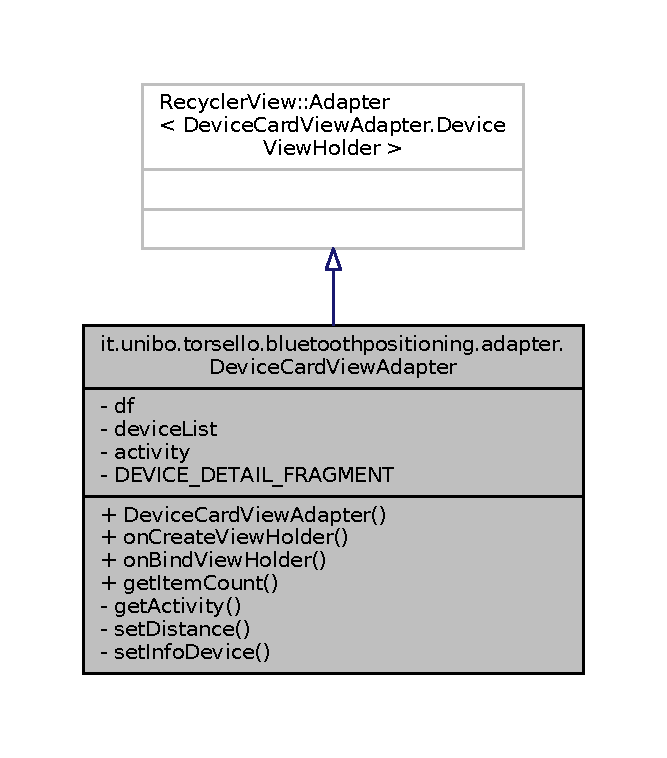
\includegraphics[width=320pt]{classit_1_1unibo_1_1torsello_1_1bluetoothpositioning_1_1adapter_1_1DeviceCardViewAdapter__inherit__graph}
\end{center}
\end{figure}


Diagramma di collaborazione per it.\+unibo.\+torsello.\+bluetoothpositioning.\+adapter.\+Device\+Card\+View\+Adapter\+:
\nopagebreak
\begin{figure}[H]
\begin{center}
\leavevmode
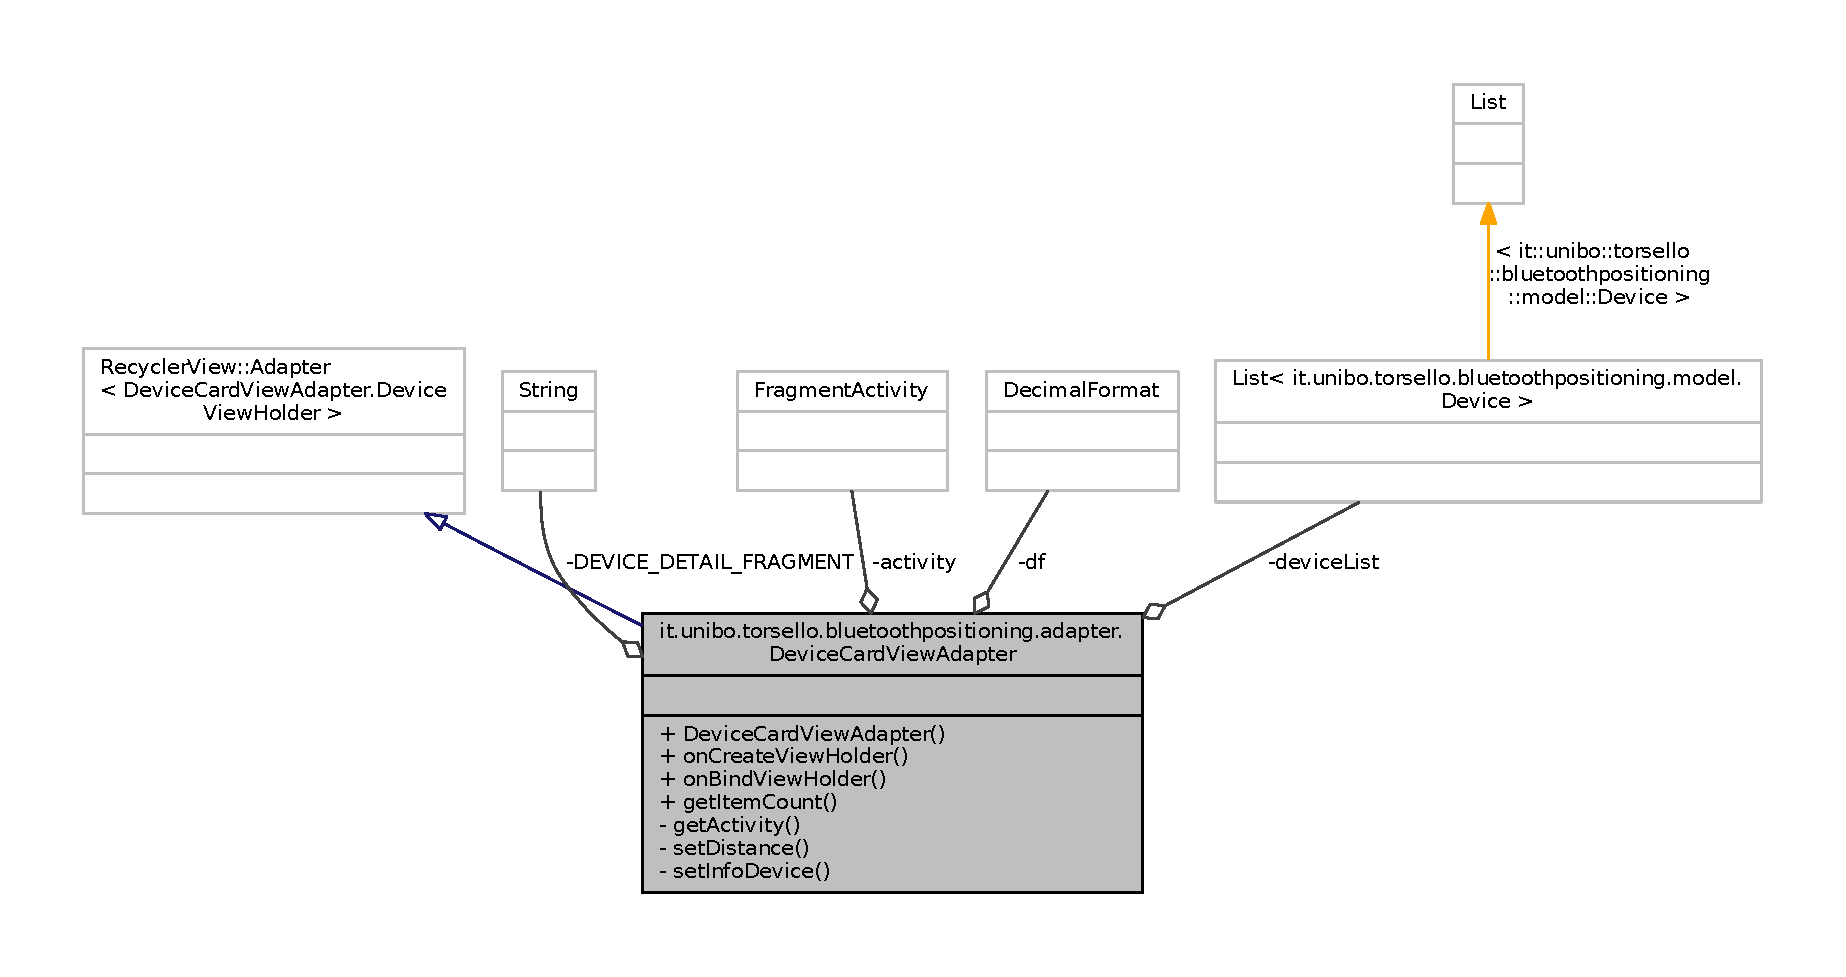
\includegraphics[width=350pt]{classit_1_1unibo_1_1torsello_1_1bluetoothpositioning_1_1adapter_1_1DeviceCardViewAdapter__coll__graph}
\end{center}
\end{figure}
\subsubsection*{Composti}
\begin{DoxyCompactItemize}
\item 
class \hyperlink{classit_1_1unibo_1_1torsello_1_1bluetoothpositioning_1_1adapter_1_1DeviceCardViewAdapter_1_1DeviceViewHolder}{Device\+View\+Holder}
\end{DoxyCompactItemize}
\subsubsection*{Membri pubblici}
\begin{DoxyCompactItemize}
\item 
\hyperlink{classit_1_1unibo_1_1torsello_1_1bluetoothpositioning_1_1adapter_1_1DeviceCardViewAdapter_a5f15271cd20868ac66c3c0876adca536_a5f15271cd20868ac66c3c0876adca536}{Device\+Card\+View\+Adapter} (final Fragment\+Activity fragment\+Activity, List$<$ \hyperlink{classit_1_1unibo_1_1torsello_1_1bluetoothpositioning_1_1model_1_1Device}{Device} $>$ \hyperlink{classit_1_1unibo_1_1torsello_1_1bluetoothpositioning_1_1adapter_1_1DeviceCardViewAdapter_a72413f87c723c585bd1ad9bc5711cf39_a72413f87c723c585bd1ad9bc5711cf39}{device\+List})
\item 
\hyperlink{classit_1_1unibo_1_1torsello_1_1bluetoothpositioning_1_1adapter_1_1DeviceCardViewAdapter_1_1DeviceViewHolder}{Device\+View\+Holder} \hyperlink{classit_1_1unibo_1_1torsello_1_1bluetoothpositioning_1_1adapter_1_1DeviceCardViewAdapter_a41227667123e30333d534b562a889229_a41227667123e30333d534b562a889229}{on\+Create\+View\+Holder} (View\+Group parent, int view\+Type)
\item 
void \hyperlink{classit_1_1unibo_1_1torsello_1_1bluetoothpositioning_1_1adapter_1_1DeviceCardViewAdapter_a3785bbe8696e1af4d8fb24e7058aa413_a3785bbe8696e1af4d8fb24e7058aa413}{on\+Bind\+View\+Holder} (\hyperlink{classit_1_1unibo_1_1torsello_1_1bluetoothpositioning_1_1adapter_1_1DeviceCardViewAdapter_1_1DeviceViewHolder}{Device\+View\+Holder} holder, final int position)
\item 
int \hyperlink{classit_1_1unibo_1_1torsello_1_1bluetoothpositioning_1_1adapter_1_1DeviceCardViewAdapter_ac039d50f397db6d5af06ca534e3e59a9_ac039d50f397db6d5af06ca534e3e59a9}{get\+Item\+Count} ()
\end{DoxyCompactItemize}
\subsubsection*{Membri privati}
\begin{DoxyCompactItemize}
\item 
Fragment\+Activity \hyperlink{classit_1_1unibo_1_1torsello_1_1bluetoothpositioning_1_1adapter_1_1DeviceCardViewAdapter_a0ff32c6bf5d84b68021bf586d64cacaf_a0ff32c6bf5d84b68021bf586d64cacaf}{get\+Activity} ()
\item 
void \hyperlink{classit_1_1unibo_1_1torsello_1_1bluetoothpositioning_1_1adapter_1_1DeviceCardViewAdapter_a8d5baa2d386a92ba4fb20b71e6e517f9_a8d5baa2d386a92ba4fb20b71e6e517f9}{set\+Distance} (\hyperlink{classit_1_1unibo_1_1torsello_1_1bluetoothpositioning_1_1adapter_1_1DeviceCardViewAdapter_1_1DeviceViewHolder}{Device\+View\+Holder} holder, \hyperlink{classit_1_1unibo_1_1torsello_1_1bluetoothpositioning_1_1model_1_1Device}{Device} device)
\item 
void \hyperlink{classit_1_1unibo_1_1torsello_1_1bluetoothpositioning_1_1adapter_1_1DeviceCardViewAdapter_aa43ee1f594b3489f6e9e4b8e20ea1612_aa43ee1f594b3489f6e9e4b8e20ea1612}{set\+Info\+Device} (\hyperlink{classit_1_1unibo_1_1torsello_1_1bluetoothpositioning_1_1adapter_1_1DeviceCardViewAdapter_1_1DeviceViewHolder}{Device\+View\+Holder} holder, Beacon beacon)
\end{DoxyCompactItemize}
\subsubsection*{Attributi privati}
\begin{DoxyCompactItemize}
\item 
Decimal\+Format \hyperlink{classit_1_1unibo_1_1torsello_1_1bluetoothpositioning_1_1adapter_1_1DeviceCardViewAdapter_ae3a2fe6b4e69e1f9b8edfb9bcba14057_ae3a2fe6b4e69e1f9b8edfb9bcba14057}{df}
\item 
List$<$ \hyperlink{classit_1_1unibo_1_1torsello_1_1bluetoothpositioning_1_1model_1_1Device}{Device} $>$ \hyperlink{classit_1_1unibo_1_1torsello_1_1bluetoothpositioning_1_1adapter_1_1DeviceCardViewAdapter_a72413f87c723c585bd1ad9bc5711cf39_a72413f87c723c585bd1ad9bc5711cf39}{device\+List}
\item 
Fragment\+Activity \hyperlink{classit_1_1unibo_1_1torsello_1_1bluetoothpositioning_1_1adapter_1_1DeviceCardViewAdapter_ad9b0572ad094da8225f1c2024ac2eb61_ad9b0572ad094da8225f1c2024ac2eb61}{activity}
\end{DoxyCompactItemize}
\subsubsection*{Attributi privati statici}
\begin{DoxyCompactItemize}
\item 
static final String \hyperlink{classit_1_1unibo_1_1torsello_1_1bluetoothpositioning_1_1adapter_1_1DeviceCardViewAdapter_a0d362081de4afb44abc82197aa597a18_a0d362081de4afb44abc82197aa597a18}{D\+E\+V\+I\+C\+E\+\_\+\+D\+E\+T\+A\+I\+L\+\_\+\+F\+R\+A\+G\+M\+E\+NT} = \char`\"{}device detail\char`\"{}
\end{DoxyCompactItemize}


\subsubsection{Descrizione dettagliata}
Created by Federico Torsello. \href{mailto:federico.torsello@studio.unibo.it}{\tt federico.\+torsello@studio.\+unibo.\+it} 

\subsubsection{Documentazione dei costruttori e dei distruttori}
\hypertarget{classit_1_1unibo_1_1torsello_1_1bluetoothpositioning_1_1adapter_1_1DeviceCardViewAdapter_a5f15271cd20868ac66c3c0876adca536_a5f15271cd20868ac66c3c0876adca536}{}\label{classit_1_1unibo_1_1torsello_1_1bluetoothpositioning_1_1adapter_1_1DeviceCardViewAdapter_a5f15271cd20868ac66c3c0876adca536_a5f15271cd20868ac66c3c0876adca536} 
\index{it\+::unibo\+::torsello\+::bluetoothpositioning\+::adapter\+::\+Device\+Card\+View\+Adapter@{it\+::unibo\+::torsello\+::bluetoothpositioning\+::adapter\+::\+Device\+Card\+View\+Adapter}!Device\+Card\+View\+Adapter@{Device\+Card\+View\+Adapter}}
\index{Device\+Card\+View\+Adapter@{Device\+Card\+View\+Adapter}!it\+::unibo\+::torsello\+::bluetoothpositioning\+::adapter\+::\+Device\+Card\+View\+Adapter@{it\+::unibo\+::torsello\+::bluetoothpositioning\+::adapter\+::\+Device\+Card\+View\+Adapter}}
\paragraph{\texorpdfstring{Device\+Card\+View\+Adapter()}{DeviceCardViewAdapter()}}
{\footnotesize\ttfamily it.\+unibo.\+torsello.\+bluetoothpositioning.\+adapter.\+Device\+Card\+View\+Adapter.\+Device\+Card\+View\+Adapter (\begin{DoxyParamCaption}\item[{final Fragment\+Activity}]{fragment\+Activity,  }\item[{List$<$ \hyperlink{classit_1_1unibo_1_1torsello_1_1bluetoothpositioning_1_1model_1_1Device}{Device} $>$}]{device\+List }\end{DoxyParamCaption})}


\begin{DoxyCode}
38                                                                                                    \{
39 
40         this.\hyperlink{classit_1_1unibo_1_1torsello_1_1bluetoothpositioning_1_1adapter_1_1DeviceCardViewAdapter_a72413f87c723c585bd1ad9bc5711cf39_a72413f87c723c585bd1ad9bc5711cf39}{deviceList} = \textcolor{keyword}{new} ArrayList<>();
41         this.\hyperlink{classit_1_1unibo_1_1torsello_1_1bluetoothpositioning_1_1adapter_1_1DeviceCardViewAdapter_a72413f87c723c585bd1ad9bc5711cf39_a72413f87c723c585bd1ad9bc5711cf39}{deviceList} = \hyperlink{classit_1_1unibo_1_1torsello_1_1bluetoothpositioning_1_1adapter_1_1DeviceCardViewAdapter_a72413f87c723c585bd1ad9bc5711cf39_a72413f87c723c585bd1ad9bc5711cf39}{deviceList};
42         this.\hyperlink{classit_1_1unibo_1_1torsello_1_1bluetoothpositioning_1_1adapter_1_1DeviceCardViewAdapter_ad9b0572ad094da8225f1c2024ac2eb61_ad9b0572ad094da8225f1c2024ac2eb61}{activity} = fragmentActivity;
43 
44         \hyperlink{classit_1_1unibo_1_1torsello_1_1bluetoothpositioning_1_1adapter_1_1DeviceCardViewAdapter_ae3a2fe6b4e69e1f9b8edfb9bcba14057_ae3a2fe6b4e69e1f9b8edfb9bcba14057}{df} = \textcolor{keyword}{new} DecimalFormat(\textcolor{stringliteral}{"0.00"}, DecimalFormatSymbols.getInstance());
45     \}
\end{DoxyCode}


\subsubsection{Documentazione delle funzioni membro}
\hypertarget{classit_1_1unibo_1_1torsello_1_1bluetoothpositioning_1_1adapter_1_1DeviceCardViewAdapter_a0ff32c6bf5d84b68021bf586d64cacaf_a0ff32c6bf5d84b68021bf586d64cacaf}{}\label{classit_1_1unibo_1_1torsello_1_1bluetoothpositioning_1_1adapter_1_1DeviceCardViewAdapter_a0ff32c6bf5d84b68021bf586d64cacaf_a0ff32c6bf5d84b68021bf586d64cacaf} 
\index{it\+::unibo\+::torsello\+::bluetoothpositioning\+::adapter\+::\+Device\+Card\+View\+Adapter@{it\+::unibo\+::torsello\+::bluetoothpositioning\+::adapter\+::\+Device\+Card\+View\+Adapter}!get\+Activity@{get\+Activity}}
\index{get\+Activity@{get\+Activity}!it\+::unibo\+::torsello\+::bluetoothpositioning\+::adapter\+::\+Device\+Card\+View\+Adapter@{it\+::unibo\+::torsello\+::bluetoothpositioning\+::adapter\+::\+Device\+Card\+View\+Adapter}}
\paragraph{\texorpdfstring{get\+Activity()}{getActivity()}}
{\footnotesize\ttfamily Fragment\+Activity it.\+unibo.\+torsello.\+bluetoothpositioning.\+adapter.\+Device\+Card\+View\+Adapter.\+get\+Activity (\begin{DoxyParamCaption}{ }\end{DoxyParamCaption})\hspace{0.3cm}{\ttfamily [private]}}


\begin{DoxyCode}
47                                            \{
48         \textcolor{keywordflow}{return} \hyperlink{classit_1_1unibo_1_1torsello_1_1bluetoothpositioning_1_1adapter_1_1DeviceCardViewAdapter_ad9b0572ad094da8225f1c2024ac2eb61_ad9b0572ad094da8225f1c2024ac2eb61}{activity};
49     \}
\end{DoxyCode}
\hypertarget{classit_1_1unibo_1_1torsello_1_1bluetoothpositioning_1_1adapter_1_1DeviceCardViewAdapter_ac039d50f397db6d5af06ca534e3e59a9_ac039d50f397db6d5af06ca534e3e59a9}{}\label{classit_1_1unibo_1_1torsello_1_1bluetoothpositioning_1_1adapter_1_1DeviceCardViewAdapter_ac039d50f397db6d5af06ca534e3e59a9_ac039d50f397db6d5af06ca534e3e59a9} 
\index{it\+::unibo\+::torsello\+::bluetoothpositioning\+::adapter\+::\+Device\+Card\+View\+Adapter@{it\+::unibo\+::torsello\+::bluetoothpositioning\+::adapter\+::\+Device\+Card\+View\+Adapter}!get\+Item\+Count@{get\+Item\+Count}}
\index{get\+Item\+Count@{get\+Item\+Count}!it\+::unibo\+::torsello\+::bluetoothpositioning\+::adapter\+::\+Device\+Card\+View\+Adapter@{it\+::unibo\+::torsello\+::bluetoothpositioning\+::adapter\+::\+Device\+Card\+View\+Adapter}}
\paragraph{\texorpdfstring{get\+Item\+Count()}{getItemCount()}}
{\footnotesize\ttfamily int it.\+unibo.\+torsello.\+bluetoothpositioning.\+adapter.\+Device\+Card\+View\+Adapter.\+get\+Item\+Count (\begin{DoxyParamCaption}{ }\end{DoxyParamCaption})}


\begin{DoxyCode}
223                               \{
224         \textcolor{keywordflow}{return} \hyperlink{classit_1_1unibo_1_1torsello_1_1bluetoothpositioning_1_1adapter_1_1DeviceCardViewAdapter_a72413f87c723c585bd1ad9bc5711cf39_a72413f87c723c585bd1ad9bc5711cf39}{deviceList}.size();
225     \}
\end{DoxyCode}
\hypertarget{classit_1_1unibo_1_1torsello_1_1bluetoothpositioning_1_1adapter_1_1DeviceCardViewAdapter_a3785bbe8696e1af4d8fb24e7058aa413_a3785bbe8696e1af4d8fb24e7058aa413}{}\label{classit_1_1unibo_1_1torsello_1_1bluetoothpositioning_1_1adapter_1_1DeviceCardViewAdapter_a3785bbe8696e1af4d8fb24e7058aa413_a3785bbe8696e1af4d8fb24e7058aa413} 
\index{it\+::unibo\+::torsello\+::bluetoothpositioning\+::adapter\+::\+Device\+Card\+View\+Adapter@{it\+::unibo\+::torsello\+::bluetoothpositioning\+::adapter\+::\+Device\+Card\+View\+Adapter}!on\+Bind\+View\+Holder@{on\+Bind\+View\+Holder}}
\index{on\+Bind\+View\+Holder@{on\+Bind\+View\+Holder}!it\+::unibo\+::torsello\+::bluetoothpositioning\+::adapter\+::\+Device\+Card\+View\+Adapter@{it\+::unibo\+::torsello\+::bluetoothpositioning\+::adapter\+::\+Device\+Card\+View\+Adapter}}
\paragraph{\texorpdfstring{on\+Bind\+View\+Holder()}{onBindViewHolder()}}
{\footnotesize\ttfamily void it.\+unibo.\+torsello.\+bluetoothpositioning.\+adapter.\+Device\+Card\+View\+Adapter.\+on\+Bind\+View\+Holder (\begin{DoxyParamCaption}\item[{\hyperlink{classit_1_1unibo_1_1torsello_1_1bluetoothpositioning_1_1adapter_1_1DeviceCardViewAdapter_1_1DeviceViewHolder}{Device\+View\+Holder}}]{holder,  }\item[{final int}]{position }\end{DoxyParamCaption})}


\begin{DoxyCode}
60                                                                               \{
61 
62         \textcolor{keyword}{final} Beacon beacon = \hyperlink{classit_1_1unibo_1_1torsello_1_1bluetoothpositioning_1_1adapter_1_1DeviceCardViewAdapter_a72413f87c723c585bd1ad9bc5711cf39_a72413f87c723c585bd1ad9bc5711cf39}{deviceList}.get(position).getBeacon();
63         \textcolor{keyword}{final} Device device = \hyperlink{classit_1_1unibo_1_1torsello_1_1bluetoothpositioning_1_1adapter_1_1DeviceCardViewAdapter_a72413f87c723c585bd1ad9bc5711cf39_a72413f87c723c585bd1ad9bc5711cf39}{deviceList}.get(position);
64 
65         \hyperlink{classit_1_1unibo_1_1torsello_1_1bluetoothpositioning_1_1adapter_1_1DeviceCardViewAdapter_aa43ee1f594b3489f6e9e4b8e20ea1612_aa43ee1f594b3489f6e9e4b8e20ea1612}{setInfoDevice}(holder, beacon);
66 
67         \hyperlink{classit_1_1unibo_1_1torsello_1_1bluetoothpositioning_1_1adapter_1_1DeviceCardViewAdapter_a8d5baa2d386a92ba4fb20b71e6e517f9_a8d5baa2d386a92ba4fb20b71e6e517f9}{setDistance}(holder, device);
68 
69         \textcolor{keyword}{final} Integer imageBeacon = device.getImageBeacon();
70         \textcolor{keywordflow}{if} (imageBeacon != null) \{
71             holder.imageView.setImageResource(imageBeacon);
72         \} \textcolor{keywordflow}{else} \{
73             holder.imageView.setImageResource(R.drawable.beacon\_unknown);
74         \}
75 
76         holder.rssiTextView.setText(String.format(\textcolor{stringliteral}{"%sdb"}, beacon.getTxPower()));
77 
78         holder.txPowerTextView.setText(String.format(\textcolor{stringliteral}{"%sdb"}, beacon.getRssi()));
79 
80         \textcolor{keyword}{final} String friendlyName = device.getFriendlyName();
81         \textcolor{keywordflow}{if} (friendlyName != null) \{
82             holder.friendlyNameTextView.setText(friendlyName);
83         \} \textcolor{keywordflow}{else} \{
84             holder.friendlyNameTextView.setText(android.R.string.unknownName);
85         \}
86 
87         \textcolor{keyword}{final} String bluetoothName = beacon.getBluetoothName();
88         \textcolor{keywordflow}{if} (bluetoothName != null) \{
89             holder.defaultNameTextView.setText(bluetoothName);
90         \} \textcolor{keywordflow}{else} \{
91             holder.defaultNameTextView.setText(android.R.string.unknownName);
92         \}
93 
94         \textcolor{keyword}{final} String macAddress = beacon.getBluetoothAddress();
95         \textcolor{keywordflow}{if} (macAddress != null) \{
96             holder.macTextView.setText(macAddress);
97         \} \textcolor{keywordflow}{else} \{
98             holder.macTextView.setText(android.R.string.unknownName);
99         \}
100 
101         \textcolor{keyword}{final} String proximity = device.getProximity();
102         \textcolor{keywordflow}{if} (proximity != null) \{
103             holder.proximityTextView.setText(proximity);
104         \} \textcolor{keywordflow}{else} \{
105             holder.proximityTextView.setText(android.R.string.unknownName);
106         \}
107 
108         \textcolor{keyword}{final} Integer color = device.getColor();
109         \textcolor{keywordflow}{if} (color != null) \{
110             holder.colorTextView.setText(color);
111         \} \textcolor{keywordflow}{else} \{
112             holder.colorTextView.setText(android.R.string.unknownName);
113         \}
114 
115         holder.view.setOnClickListener(\textcolor{keyword}{new} View.OnClickListener() \{
116             @Override
117             \textcolor{keyword}{public} \textcolor{keywordtype}{void} onClick(View v) \{
118                 \textcolor{keyword}{final} String deviceDetailName;
119                 \textcolor{keywordflow}{if} (device.getFriendlyName() != null) \{
120                     deviceDetailName = device.getFriendlyName();
121                 \} \textcolor{keywordflow}{else} \{
122                     deviceDetailName = device.getAddress();
123                 \}
124 
125                 \textcolor{keyword}{new} Thread(\textcolor{keyword}{new} Runnable() \{
126                     @Override
127                     \textcolor{keyword}{public} \textcolor{keywordtype}{void} run() \{
128                         \hyperlink{classit_1_1unibo_1_1torsello_1_1bluetoothpositioning_1_1adapter_1_1DeviceCardViewAdapter_a0ff32c6bf5d84b68021bf586d64cacaf_a0ff32c6bf5d84b68021bf586d64cacaf}{getActivity}().runOnUiThread(\textcolor{keyword}{new} Runnable() \{
129                             @Override
130                             \textcolor{keyword}{public} \textcolor{keywordtype}{void} run() \{
131 
132                                 Fragment currentFrag = \hyperlink{classit_1_1unibo_1_1torsello_1_1bluetoothpositioning_1_1adapter_1_1DeviceCardViewAdapter_a0ff32c6bf5d84b68021bf586d64cacaf_a0ff32c6bf5d84b68021bf586d64cacaf}{getActivity}().getSupportFragmentManager()
133                                         .findFragmentByTag(
      \hyperlink{classit_1_1unibo_1_1torsello_1_1bluetoothpositioning_1_1adapter_1_1DeviceCardViewAdapter_a0d362081de4afb44abc82197aa597a18_a0d362081de4afb44abc82197aa597a18}{DEVICE\_DETAIL\_FRAGMENT});
134 
135                                 \textcolor{keywordflow}{if} (currentFrag == null) \{
136                                     \hyperlink{classit_1_1unibo_1_1torsello_1_1bluetoothpositioning_1_1adapter_1_1DeviceCardViewAdapter_a0ff32c6bf5d84b68021bf586d64cacaf_a0ff32c6bf5d84b68021bf586d64cacaf}{getActivity}().getSupportFragmentManager().beginTransaction()
137                                             .replace(R.id.contentMainLayout,
138                                                     DeviceDetailFragment.newInstance(deviceDetailName),
139                                                     \hyperlink{classit_1_1unibo_1_1torsello_1_1bluetoothpositioning_1_1adapter_1_1DeviceCardViewAdapter_a0d362081de4afb44abc82197aa597a18_a0d362081de4afb44abc82197aa597a18}{DEVICE\_DETAIL\_FRAGMENT})
140                                             .commit();
141                                 \}
142                             \}
143                         \});
144                     \}
145                 \}).start();
146             \}
147         \});
148     \}
\end{DoxyCode}
\hypertarget{classit_1_1unibo_1_1torsello_1_1bluetoothpositioning_1_1adapter_1_1DeviceCardViewAdapter_a41227667123e30333d534b562a889229_a41227667123e30333d534b562a889229}{}\label{classit_1_1unibo_1_1torsello_1_1bluetoothpositioning_1_1adapter_1_1DeviceCardViewAdapter_a41227667123e30333d534b562a889229_a41227667123e30333d534b562a889229} 
\index{it\+::unibo\+::torsello\+::bluetoothpositioning\+::adapter\+::\+Device\+Card\+View\+Adapter@{it\+::unibo\+::torsello\+::bluetoothpositioning\+::adapter\+::\+Device\+Card\+View\+Adapter}!on\+Create\+View\+Holder@{on\+Create\+View\+Holder}}
\index{on\+Create\+View\+Holder@{on\+Create\+View\+Holder}!it\+::unibo\+::torsello\+::bluetoothpositioning\+::adapter\+::\+Device\+Card\+View\+Adapter@{it\+::unibo\+::torsello\+::bluetoothpositioning\+::adapter\+::\+Device\+Card\+View\+Adapter}}
\paragraph{\texorpdfstring{on\+Create\+View\+Holder()}{onCreateViewHolder()}}
{\footnotesize\ttfamily \hyperlink{classit_1_1unibo_1_1torsello_1_1bluetoothpositioning_1_1adapter_1_1DeviceCardViewAdapter_1_1DeviceViewHolder}{Device\+View\+Holder} it.\+unibo.\+torsello.\+bluetoothpositioning.\+adapter.\+Device\+Card\+View\+Adapter.\+on\+Create\+View\+Holder (\begin{DoxyParamCaption}\item[{View\+Group}]{parent,  }\item[{int}]{view\+Type }\end{DoxyParamCaption})}


\begin{DoxyCode}
52                                                                                \{
53 
54         View root = LayoutInflater.from(parent.getContext())
55                 .inflate(R.layout.list\_items, parent, \textcolor{keyword}{false});
56         \textcolor{keywordflow}{return} \textcolor{keyword}{new} DeviceViewHolder(root);
57     \}
\end{DoxyCode}
\hypertarget{classit_1_1unibo_1_1torsello_1_1bluetoothpositioning_1_1adapter_1_1DeviceCardViewAdapter_a8d5baa2d386a92ba4fb20b71e6e517f9_a8d5baa2d386a92ba4fb20b71e6e517f9}{}\label{classit_1_1unibo_1_1torsello_1_1bluetoothpositioning_1_1adapter_1_1DeviceCardViewAdapter_a8d5baa2d386a92ba4fb20b71e6e517f9_a8d5baa2d386a92ba4fb20b71e6e517f9} 
\index{it\+::unibo\+::torsello\+::bluetoothpositioning\+::adapter\+::\+Device\+Card\+View\+Adapter@{it\+::unibo\+::torsello\+::bluetoothpositioning\+::adapter\+::\+Device\+Card\+View\+Adapter}!set\+Distance@{set\+Distance}}
\index{set\+Distance@{set\+Distance}!it\+::unibo\+::torsello\+::bluetoothpositioning\+::adapter\+::\+Device\+Card\+View\+Adapter@{it\+::unibo\+::torsello\+::bluetoothpositioning\+::adapter\+::\+Device\+Card\+View\+Adapter}}
\paragraph{\texorpdfstring{set\+Distance()}{setDistance()}}
{\footnotesize\ttfamily void it.\+unibo.\+torsello.\+bluetoothpositioning.\+adapter.\+Device\+Card\+View\+Adapter.\+set\+Distance (\begin{DoxyParamCaption}\item[{\hyperlink{classit_1_1unibo_1_1torsello_1_1bluetoothpositioning_1_1adapter_1_1DeviceCardViewAdapter_1_1DeviceViewHolder}{Device\+View\+Holder}}]{holder,  }\item[{\hyperlink{classit_1_1unibo_1_1torsello_1_1bluetoothpositioning_1_1model_1_1Device}{Device}}]{device }\end{DoxyParamCaption})\hspace{0.3cm}{\ttfamily [private]}}


\begin{DoxyCode}
150                                                                      \{
151         holder.altbeaconDistanceTextView.setText(String.format(\textcolor{stringliteral}{"%sm"}, \hyperlink{classit_1_1unibo_1_1torsello_1_1bluetoothpositioning_1_1adapter_1_1DeviceCardViewAdapter_ae3a2fe6b4e69e1f9b8edfb9bcba14057_ae3a2fe6b4e69e1f9b8edfb9bcba14057}{df}.format(device.
      getAltBeaconDistance())));
152 
153         holder.standardRawDistanceTextView.setText(String.format(\textcolor{stringliteral}{"%sm"}, \hyperlink{classit_1_1unibo_1_1torsello_1_1bluetoothpositioning_1_1adapter_1_1DeviceCardViewAdapter_ae3a2fe6b4e69e1f9b8edfb9bcba14057_ae3a2fe6b4e69e1f9b8edfb9bcba14057}{df}.format(device.getRawDistance()
      )));
154 
155         \textcolor{keywordflow}{if} (!device.isKalmanFilterEnabled())\{
156             holder.kalmanFilterDistanceTextView.setText(\hyperlink{classit_1_1unibo_1_1torsello_1_1bluetoothpositioning_1_1adapter_1_1DeviceCardViewAdapter_a0ff32c6bf5d84b68021bf586d64cacaf_a0ff32c6bf5d84b68021bf586d64cacaf}{getActivity}().getText(R.string.
      kalman\_filter\_disabled));
157         \} \textcolor{keywordflow}{else} \{
158             holder.kalmanFilterDistanceTextView.setText(String.format(\textcolor{stringliteral}{"%s"}, \hyperlink{classit_1_1unibo_1_1torsello_1_1bluetoothpositioning_1_1adapter_1_1DeviceCardViewAdapter_ae3a2fe6b4e69e1f9b8edfb9bcba14057_ae3a2fe6b4e69e1f9b8edfb9bcba14057}{df}.format(device.
      getKalmanFilterDistance())));
159         \}
160     \}
\end{DoxyCode}
\hypertarget{classit_1_1unibo_1_1torsello_1_1bluetoothpositioning_1_1adapter_1_1DeviceCardViewAdapter_aa43ee1f594b3489f6e9e4b8e20ea1612_aa43ee1f594b3489f6e9e4b8e20ea1612}{}\label{classit_1_1unibo_1_1torsello_1_1bluetoothpositioning_1_1adapter_1_1DeviceCardViewAdapter_aa43ee1f594b3489f6e9e4b8e20ea1612_aa43ee1f594b3489f6e9e4b8e20ea1612} 
\index{it\+::unibo\+::torsello\+::bluetoothpositioning\+::adapter\+::\+Device\+Card\+View\+Adapter@{it\+::unibo\+::torsello\+::bluetoothpositioning\+::adapter\+::\+Device\+Card\+View\+Adapter}!set\+Info\+Device@{set\+Info\+Device}}
\index{set\+Info\+Device@{set\+Info\+Device}!it\+::unibo\+::torsello\+::bluetoothpositioning\+::adapter\+::\+Device\+Card\+View\+Adapter@{it\+::unibo\+::torsello\+::bluetoothpositioning\+::adapter\+::\+Device\+Card\+View\+Adapter}}
\paragraph{\texorpdfstring{set\+Info\+Device()}{setInfoDevice()}}
{\footnotesize\ttfamily void it.\+unibo.\+torsello.\+bluetoothpositioning.\+adapter.\+Device\+Card\+View\+Adapter.\+set\+Info\+Device (\begin{DoxyParamCaption}\item[{\hyperlink{classit_1_1unibo_1_1torsello_1_1bluetoothpositioning_1_1adapter_1_1DeviceCardViewAdapter_1_1DeviceViewHolder}{Device\+View\+Holder}}]{holder,  }\item[{Beacon}]{beacon }\end{DoxyParamCaption})\hspace{0.3cm}{\ttfamily [private]}}


\begin{DoxyCode}
162                                                                        \{
163         \textcolor{keywordflow}{if} (beacon.getServiceUuid() == 0xfeaa) \{
164 
165             holder.visibilityUUIDLinearLayout.setVisibility(View.GONE);
166             holder.visibilityNameSpaceLinearLayout.setVisibility(View.VISIBLE);
167 
168             \textcolor{keywordflow}{if} (beacon.getBeaconTypeCode() == 0x00) \{
169                 \textcolor{comment}{// Eddystone-UID}
170                 \textcolor{keywordflow}{if} (beacon.getId1() != null) \{
171                     holder.nameSpaceTextView.setText(beacon.getId1().toString());
172                 \} \textcolor{keywordflow}{else} \{
173                     holder.nameSpaceTextView.setText(android.R.string.unknownName);
174                 \}
175 
176                 \textcolor{keywordflow}{if} (beacon.getId2() != null) \{
177                     holder.instanceTextView.setText(beacon.getId2().toString());
178                 \} \textcolor{keywordflow}{else} \{
179                     holder.instanceTextView.setText(android.R.string.unknownName);
180                 \}
181 
182             \} \textcolor{keywordflow}{else} \textcolor{keywordflow}{if} (beacon.getBeaconTypeCode() == 0x10) \{
183                 \textcolor{comment}{// Eddystone-URL}
184                 \textcolor{comment}{// String url = UrlBeaconUrlCompressor.uncompress(beacon.getId1().toByteArray());}
185             \} \textcolor{keywordflow}{else} \textcolor{keywordflow}{if} (beacon.getBeaconTypeCode() == 0x20) \{
186                 \textcolor{keywordflow}{if} (!beacon.getExtraDataFields().isEmpty()) \{
187                     \textcolor{comment}{// Eddystone-TLM}
188                 \}
189             \}
190         \} \textcolor{keywordflow}{else} \textcolor{keywordflow}{if} (beacon.getServiceUuid() == 0xbeac) \{
191             \textcolor{comment}{// AltBeacon}
192         \} \textcolor{keywordflow}{else} \textcolor{keywordflow}{if} (beacon.getBeaconTypeCode() == 0x0215) \{ \textcolor{comment}{//533 in dec)}
193 
194             holder.visibilityUUIDLinearLayout.setVisibility(View.VISIBLE);
195             holder.visibilityNameSpaceLinearLayout.setVisibility(View.GONE);
196 
197             \textcolor{comment}{// AppleIBeacon}
198             \textcolor{keywordflow}{if} (beacon.getId1() != null) \{
199                 holder.uuidTextView.setText(beacon.getId1().toString());
200             \} \textcolor{keywordflow}{else} \{
201                 holder.uuidTextView.setText(android.R.string.unknownName);
202             \}
203 
204             \textcolor{keywordflow}{if} (beacon.getId2() != null) \{
205                 holder.majorTextView.setText(beacon.getId2().toString());
206             \} \textcolor{keywordflow}{else} \{
207                 holder.majorTextView.setText(android.R.string.unknownName);
208             \}
209 
210             \textcolor{keywordflow}{if} (beacon.getId3() != null) \{
211                 holder.minorTextView.setText(beacon.getId3().toString());
212             \} \textcolor{keywordflow}{else} \{
213                 holder.minorTextView.setText(android.R.string.unknownName);
214             \}
215 
216         \} \textcolor{keywordflow}{else} \textcolor{keywordflow}{if} (beacon.getBeaconTypeCode() == 0x0101) \{
217             \textcolor{comment}{// EstimoteNearable}
218         \}
219 
220     \}
\end{DoxyCode}


\subsubsection{Documentazione dei membri dato}
\hypertarget{classit_1_1unibo_1_1torsello_1_1bluetoothpositioning_1_1adapter_1_1DeviceCardViewAdapter_ad9b0572ad094da8225f1c2024ac2eb61_ad9b0572ad094da8225f1c2024ac2eb61}{}\label{classit_1_1unibo_1_1torsello_1_1bluetoothpositioning_1_1adapter_1_1DeviceCardViewAdapter_ad9b0572ad094da8225f1c2024ac2eb61_ad9b0572ad094da8225f1c2024ac2eb61} 
\index{it\+::unibo\+::torsello\+::bluetoothpositioning\+::adapter\+::\+Device\+Card\+View\+Adapter@{it\+::unibo\+::torsello\+::bluetoothpositioning\+::adapter\+::\+Device\+Card\+View\+Adapter}!activity@{activity}}
\index{activity@{activity}!it\+::unibo\+::torsello\+::bluetoothpositioning\+::adapter\+::\+Device\+Card\+View\+Adapter@{it\+::unibo\+::torsello\+::bluetoothpositioning\+::adapter\+::\+Device\+Card\+View\+Adapter}}
\paragraph{\texorpdfstring{activity}{activity}}
{\footnotesize\ttfamily Fragment\+Activity it.\+unibo.\+torsello.\+bluetoothpositioning.\+adapter.\+Device\+Card\+View\+Adapter.\+activity\hspace{0.3cm}{\ttfamily [private]}}

\hypertarget{classit_1_1unibo_1_1torsello_1_1bluetoothpositioning_1_1adapter_1_1DeviceCardViewAdapter_a0d362081de4afb44abc82197aa597a18_a0d362081de4afb44abc82197aa597a18}{}\label{classit_1_1unibo_1_1torsello_1_1bluetoothpositioning_1_1adapter_1_1DeviceCardViewAdapter_a0d362081de4afb44abc82197aa597a18_a0d362081de4afb44abc82197aa597a18} 
\index{it\+::unibo\+::torsello\+::bluetoothpositioning\+::adapter\+::\+Device\+Card\+View\+Adapter@{it\+::unibo\+::torsello\+::bluetoothpositioning\+::adapter\+::\+Device\+Card\+View\+Adapter}!D\+E\+V\+I\+C\+E\+\_\+\+D\+E\+T\+A\+I\+L\+\_\+\+F\+R\+A\+G\+M\+E\+NT@{D\+E\+V\+I\+C\+E\+\_\+\+D\+E\+T\+A\+I\+L\+\_\+\+F\+R\+A\+G\+M\+E\+NT}}
\index{D\+E\+V\+I\+C\+E\+\_\+\+D\+E\+T\+A\+I\+L\+\_\+\+F\+R\+A\+G\+M\+E\+NT@{D\+E\+V\+I\+C\+E\+\_\+\+D\+E\+T\+A\+I\+L\+\_\+\+F\+R\+A\+G\+M\+E\+NT}!it\+::unibo\+::torsello\+::bluetoothpositioning\+::adapter\+::\+Device\+Card\+View\+Adapter@{it\+::unibo\+::torsello\+::bluetoothpositioning\+::adapter\+::\+Device\+Card\+View\+Adapter}}
\paragraph{\texorpdfstring{D\+E\+V\+I\+C\+E\+\_\+\+D\+E\+T\+A\+I\+L\+\_\+\+F\+R\+A\+G\+M\+E\+NT}{DEVICE\_DETAIL\_FRAGMENT}}
{\footnotesize\ttfamily final String it.\+unibo.\+torsello.\+bluetoothpositioning.\+adapter.\+Device\+Card\+View\+Adapter.\+D\+E\+V\+I\+C\+E\+\_\+\+D\+E\+T\+A\+I\+L\+\_\+\+F\+R\+A\+G\+M\+E\+NT = \char`\"{}device detail\char`\"{}\hspace{0.3cm}{\ttfamily [static]}, {\ttfamily [private]}}

\hypertarget{classit_1_1unibo_1_1torsello_1_1bluetoothpositioning_1_1adapter_1_1DeviceCardViewAdapter_a72413f87c723c585bd1ad9bc5711cf39_a72413f87c723c585bd1ad9bc5711cf39}{}\label{classit_1_1unibo_1_1torsello_1_1bluetoothpositioning_1_1adapter_1_1DeviceCardViewAdapter_a72413f87c723c585bd1ad9bc5711cf39_a72413f87c723c585bd1ad9bc5711cf39} 
\index{it\+::unibo\+::torsello\+::bluetoothpositioning\+::adapter\+::\+Device\+Card\+View\+Adapter@{it\+::unibo\+::torsello\+::bluetoothpositioning\+::adapter\+::\+Device\+Card\+View\+Adapter}!device\+List@{device\+List}}
\index{device\+List@{device\+List}!it\+::unibo\+::torsello\+::bluetoothpositioning\+::adapter\+::\+Device\+Card\+View\+Adapter@{it\+::unibo\+::torsello\+::bluetoothpositioning\+::adapter\+::\+Device\+Card\+View\+Adapter}}
\paragraph{\texorpdfstring{device\+List}{deviceList}}
{\footnotesize\ttfamily List$<$\hyperlink{classit_1_1unibo_1_1torsello_1_1bluetoothpositioning_1_1model_1_1Device}{Device}$>$ it.\+unibo.\+torsello.\+bluetoothpositioning.\+adapter.\+Device\+Card\+View\+Adapter.\+device\+List\hspace{0.3cm}{\ttfamily [private]}}

\hypertarget{classit_1_1unibo_1_1torsello_1_1bluetoothpositioning_1_1adapter_1_1DeviceCardViewAdapter_ae3a2fe6b4e69e1f9b8edfb9bcba14057_ae3a2fe6b4e69e1f9b8edfb9bcba14057}{}\label{classit_1_1unibo_1_1torsello_1_1bluetoothpositioning_1_1adapter_1_1DeviceCardViewAdapter_ae3a2fe6b4e69e1f9b8edfb9bcba14057_ae3a2fe6b4e69e1f9b8edfb9bcba14057} 
\index{it\+::unibo\+::torsello\+::bluetoothpositioning\+::adapter\+::\+Device\+Card\+View\+Adapter@{it\+::unibo\+::torsello\+::bluetoothpositioning\+::adapter\+::\+Device\+Card\+View\+Adapter}!df@{df}}
\index{df@{df}!it\+::unibo\+::torsello\+::bluetoothpositioning\+::adapter\+::\+Device\+Card\+View\+Adapter@{it\+::unibo\+::torsello\+::bluetoothpositioning\+::adapter\+::\+Device\+Card\+View\+Adapter}}
\paragraph{\texorpdfstring{df}{df}}
{\footnotesize\ttfamily Decimal\+Format it.\+unibo.\+torsello.\+bluetoothpositioning.\+adapter.\+Device\+Card\+View\+Adapter.\+df\hspace{0.3cm}{\ttfamily [private]}}



La documentazione per questa classe è stata generata a partire dal seguente file\+:\begin{DoxyCompactItemize}
\item 
\hyperlink{DeviceCardViewAdapter_8java}{Device\+Card\+View\+Adapter.\+java}\end{DoxyCompactItemize}

\hypertarget{classit_1_1unibo_1_1torsello_1_1bluetoothpositioning_1_1fragment_1_1devicesObservers_1_1DeviceChartFragment}{}\subsection{Riferimenti per la classe it.\+unibo.\+torsello.\+bluetoothpositioning.\+fragment.\+devices\+Observers.\+Device\+Chart\+Fragment}
\label{classit_1_1unibo_1_1torsello_1_1bluetoothpositioning_1_1fragment_1_1devicesObservers_1_1DeviceChartFragment}\index{it.\+unibo.\+torsello.\+bluetoothpositioning.\+fragment.\+devices\+Observers.\+Device\+Chart\+Fragment@{it.\+unibo.\+torsello.\+bluetoothpositioning.\+fragment.\+devices\+Observers.\+Device\+Chart\+Fragment}}


Diagramma delle classi per it.\+unibo.\+torsello.\+bluetoothpositioning.\+fragment.\+devices\+Observers.\+Device\+Chart\+Fragment
\nopagebreak
\begin{figure}[H]
\begin{center}
\leavevmode
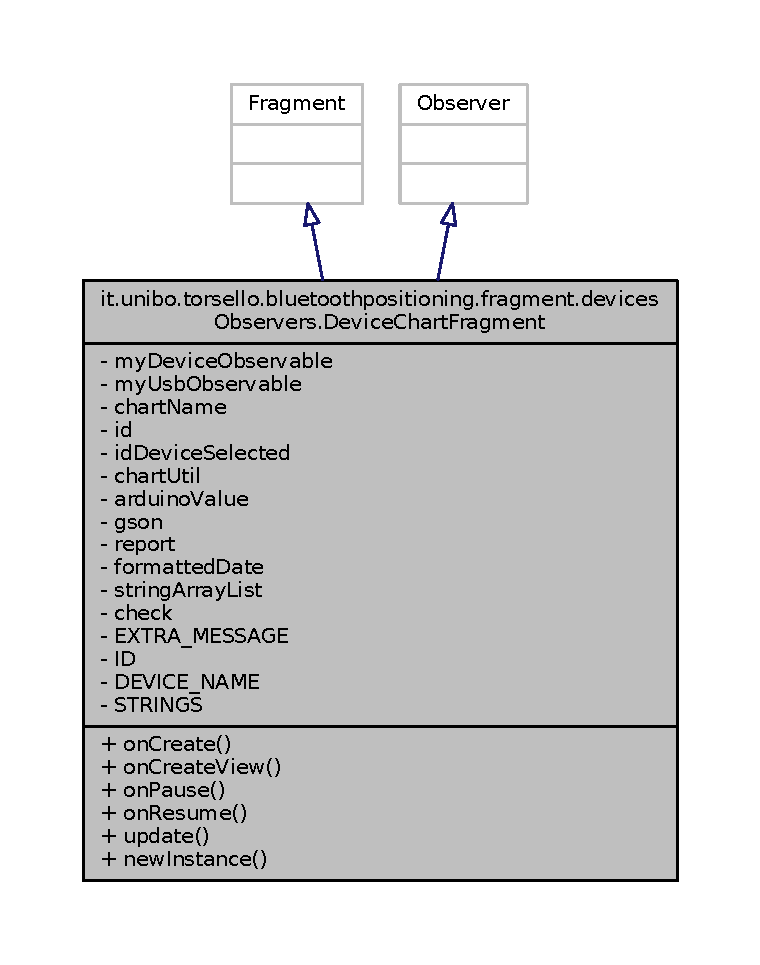
\includegraphics[width=350pt]{classit_1_1unibo_1_1torsello_1_1bluetoothpositioning_1_1fragment_1_1devicesObservers_1_1DeviceChartFragment__inherit__graph}
\end{center}
\end{figure}


Diagramma di collaborazione per it.\+unibo.\+torsello.\+bluetoothpositioning.\+fragment.\+devices\+Observers.\+Device\+Chart\+Fragment\+:
\nopagebreak
\begin{figure}[H]
\begin{center}
\leavevmode
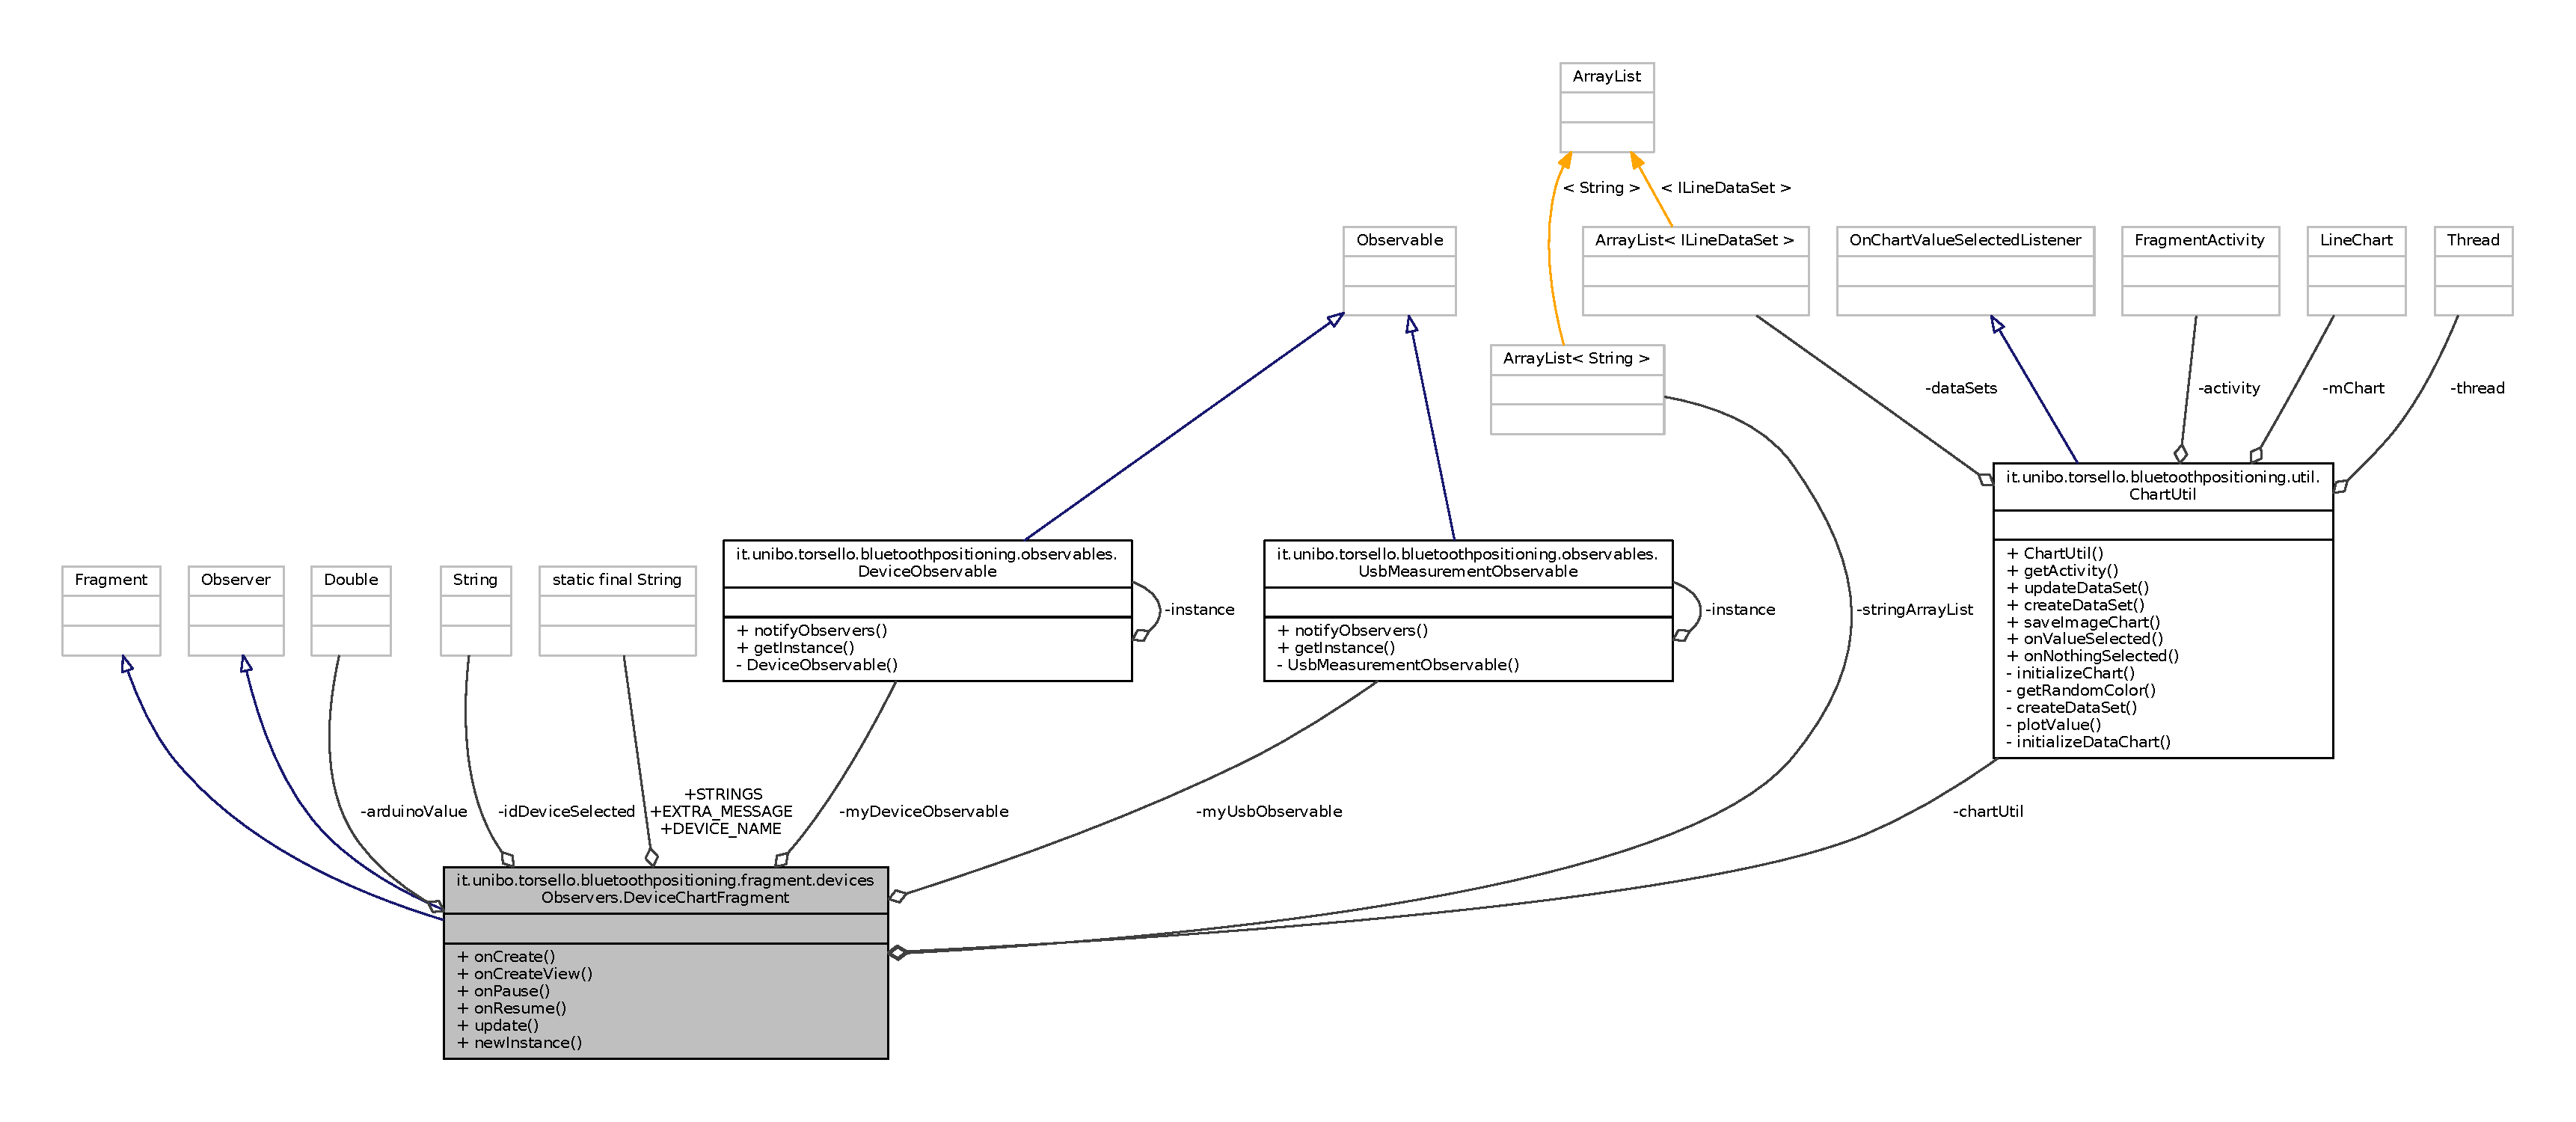
\includegraphics[width=350pt]{classit_1_1unibo_1_1torsello_1_1bluetoothpositioning_1_1fragment_1_1devicesObservers_1_1DeviceChartFragment__coll__graph}
\end{center}
\end{figure}
\subsubsection*{Membri pubblici}
\begin{DoxyCompactItemize}
\item 
void \hyperlink{classit_1_1unibo_1_1torsello_1_1bluetoothpositioning_1_1fragment_1_1devicesObservers_1_1DeviceChartFragment_a2941a5d389e0ab2c21cb96a61ba72dca_a2941a5d389e0ab2c21cb96a61ba72dca}{on\+Create} (Bundle saved\+Instance\+State)
\item 
View \hyperlink{classit_1_1unibo_1_1torsello_1_1bluetoothpositioning_1_1fragment_1_1devicesObservers_1_1DeviceChartFragment_aa9ea67b08976eaaa04d7fa197a8fe562_aa9ea67b08976eaaa04d7fa197a8fe562}{on\+Create\+View} (Layout\+Inflater inflater, View\+Group container, Bundle saved\+Instance\+State)
\item 
void \hyperlink{classit_1_1unibo_1_1torsello_1_1bluetoothpositioning_1_1fragment_1_1devicesObservers_1_1DeviceChartFragment_a25bf98c9a715f133efd2f25b2f8aeb38_a25bf98c9a715f133efd2f25b2f8aeb38}{on\+Pause} ()
\item 
void \hyperlink{classit_1_1unibo_1_1torsello_1_1bluetoothpositioning_1_1fragment_1_1devicesObservers_1_1DeviceChartFragment_ae76428fde174d312bed28057f3f66d46_ae76428fde174d312bed28057f3f66d46}{on\+Resume} ()
\item 
void \hyperlink{classit_1_1unibo_1_1torsello_1_1bluetoothpositioning_1_1fragment_1_1devicesObservers_1_1DeviceChartFragment_a83fb3f76a108192b8df7640cfafcd98d_a83fb3f76a108192b8df7640cfafcd98d}{update} (Observable o, Object arg)
\end{DoxyCompactItemize}
\subsubsection*{Membri pubblici statici}
\begin{DoxyCompactItemize}
\item 
static \hyperlink{classit_1_1unibo_1_1torsello_1_1bluetoothpositioning_1_1fragment_1_1devicesObservers_1_1DeviceChartFragment}{Device\+Chart\+Fragment} \hyperlink{classit_1_1unibo_1_1torsello_1_1bluetoothpositioning_1_1fragment_1_1devicesObservers_1_1DeviceChartFragment_ac3a29d125bf39a859054cca378274185_ac3a29d125bf39a859054cca378274185}{new\+Instance} (String message, String device\+Name, Array\+List$<$ String $>$ strings)
\end{DoxyCompactItemize}
\subsubsection*{Attributi pubblici statici}
\begin{DoxyCompactItemize}
\item 
static final String \hyperlink{classit_1_1unibo_1_1torsello_1_1bluetoothpositioning_1_1fragment_1_1devicesObservers_1_1DeviceChartFragment_a07b2f252088c2cf0af46ea39ae83bc09_a07b2f252088c2cf0af46ea39ae83bc09}{E\+X\+T\+R\+A\+\_\+\+M\+E\+S\+S\+A\+GE} = \char`\"{}E\+X\+T\+R\+A\+\_\+\+M\+E\+S\+S\+A\+GE\char`\"{}
\item 
static final String \hyperlink{classit_1_1unibo_1_1torsello_1_1bluetoothpositioning_1_1fragment_1_1devicesObservers_1_1DeviceChartFragment_a5f778eb494a70b25d52ea96e85342011_a5f778eb494a70b25d52ea96e85342011}{D\+E\+V\+I\+C\+E\+\_\+\+N\+A\+ME} = \char`\"{}D\+E\+V\+I\+C\+E\+\_\+\+N\+A\+ME\char`\"{}
\item 
static final String \hyperlink{classit_1_1unibo_1_1torsello_1_1bluetoothpositioning_1_1fragment_1_1devicesObservers_1_1DeviceChartFragment_a343835bbfb305e22881397c1b9249b00_a343835bbfb305e22881397c1b9249b00}{S\+T\+R\+I\+N\+GS} = \char`\"{}S\+T\+R\+I\+N\+GS\char`\"{}
\end{DoxyCompactItemize}
\subsubsection*{Attributi privati}
\begin{DoxyCompactItemize}
\item 
\hyperlink{classit_1_1unibo_1_1torsello_1_1bluetoothpositioning_1_1observables_1_1DeviceObservable}{Device\+Observable} \hyperlink{classit_1_1unibo_1_1torsello_1_1bluetoothpositioning_1_1fragment_1_1devicesObservers_1_1DeviceChartFragment_a2c8de6418fffdb5affe4de22185b55eb_a2c8de6418fffdb5affe4de22185b55eb}{my\+Device\+Observable}
\item 
\hyperlink{classit_1_1unibo_1_1torsello_1_1bluetoothpositioning_1_1observables_1_1UsbMeasurementObservable}{Usb\+Measurement\+Observable} \hyperlink{classit_1_1unibo_1_1torsello_1_1bluetoothpositioning_1_1fragment_1_1devicesObservers_1_1DeviceChartFragment_a577dad67b3eabc0f48e95d08e9f5881b_a577dad67b3eabc0f48e95d08e9f5881b}{my\+Usb\+Observable}
\item 
String \hyperlink{classit_1_1unibo_1_1torsello_1_1bluetoothpositioning_1_1fragment_1_1devicesObservers_1_1DeviceChartFragment_aa117a620e8f8017f213be26e321d7084_aa117a620e8f8017f213be26e321d7084}{id\+Device\+Selected}
\item 
\hyperlink{classit_1_1unibo_1_1torsello_1_1bluetoothpositioning_1_1util_1_1ChartUtil}{Chart\+Util} \hyperlink{classit_1_1unibo_1_1torsello_1_1bluetoothpositioning_1_1fragment_1_1devicesObservers_1_1DeviceChartFragment_afe4ee0e5d07f3efb6887428c9ef04a2e_afe4ee0e5d07f3efb6887428c9ef04a2e}{chart\+Util}
\item 
Double \hyperlink{classit_1_1unibo_1_1torsello_1_1bluetoothpositioning_1_1fragment_1_1devicesObservers_1_1DeviceChartFragment_a913e9b39a11d361793d7884bd2ddfd4c_a913e9b39a11d361793d7884bd2ddfd4c}{arduino\+Value} = 0D
\item 
Array\+List$<$ String $>$ \hyperlink{classit_1_1unibo_1_1torsello_1_1bluetoothpositioning_1_1fragment_1_1devicesObservers_1_1DeviceChartFragment_a7bff8d8b328464c2add8d6664c149cb5_a7bff8d8b328464c2add8d6664c149cb5}{string\+Array\+List}
\end{DoxyCompactItemize}


\subsubsection{Documentazione delle funzioni membro}
\hypertarget{classit_1_1unibo_1_1torsello_1_1bluetoothpositioning_1_1fragment_1_1devicesObservers_1_1DeviceChartFragment_ac3a29d125bf39a859054cca378274185_ac3a29d125bf39a859054cca378274185}{}\label{classit_1_1unibo_1_1torsello_1_1bluetoothpositioning_1_1fragment_1_1devicesObservers_1_1DeviceChartFragment_ac3a29d125bf39a859054cca378274185_ac3a29d125bf39a859054cca378274185} 
\index{it\+::unibo\+::torsello\+::bluetoothpositioning\+::fragment\+::devices\+Observers\+::\+Device\+Chart\+Fragment@{it\+::unibo\+::torsello\+::bluetoothpositioning\+::fragment\+::devices\+Observers\+::\+Device\+Chart\+Fragment}!new\+Instance@{new\+Instance}}
\index{new\+Instance@{new\+Instance}!it\+::unibo\+::torsello\+::bluetoothpositioning\+::fragment\+::devices\+Observers\+::\+Device\+Chart\+Fragment@{it\+::unibo\+::torsello\+::bluetoothpositioning\+::fragment\+::devices\+Observers\+::\+Device\+Chart\+Fragment}}
\paragraph{\texorpdfstring{new\+Instance()}{newInstance()}}
{\footnotesize\ttfamily static \hyperlink{classit_1_1unibo_1_1torsello_1_1bluetoothpositioning_1_1fragment_1_1devicesObservers_1_1DeviceChartFragment}{Device\+Chart\+Fragment} it.\+unibo.\+torsello.\+bluetoothpositioning.\+fragment.\+devices\+Observers.\+Device\+Chart\+Fragment.\+new\+Instance (\begin{DoxyParamCaption}\item[{String}]{message,  }\item[{String}]{device\+Name,  }\item[{Array\+List$<$ String $>$}]{strings }\end{DoxyParamCaption})\hspace{0.3cm}{\ttfamily [static]}}


\begin{DoxyCode}
40                                                                              \{
41         DeviceChartFragment fragment = \textcolor{keyword}{new} DeviceChartFragment();
42         Bundle args = \textcolor{keyword}{new} Bundle();
43         args.putString(\hyperlink{classit_1_1unibo_1_1torsello_1_1bluetoothpositioning_1_1fragment_1_1devicesObservers_1_1DeviceChartFragment_a07b2f252088c2cf0af46ea39ae83bc09_a07b2f252088c2cf0af46ea39ae83bc09}{EXTRA\_MESSAGE}, message);
44         args.putString(\hyperlink{classit_1_1unibo_1_1torsello_1_1bluetoothpositioning_1_1fragment_1_1devicesObservers_1_1DeviceChartFragment_a5f778eb494a70b25d52ea96e85342011_a5f778eb494a70b25d52ea96e85342011}{DEVICE\_NAME}, deviceName);
45         args.putStringArrayList(\hyperlink{classit_1_1unibo_1_1torsello_1_1bluetoothpositioning_1_1fragment_1_1devicesObservers_1_1DeviceChartFragment_a343835bbfb305e22881397c1b9249b00_a343835bbfb305e22881397c1b9249b00}{STRINGS}, strings);
46         fragment.setArguments(args);
47         \textcolor{keywordflow}{return} fragment;
48     \}
\end{DoxyCode}
\hypertarget{classit_1_1unibo_1_1torsello_1_1bluetoothpositioning_1_1fragment_1_1devicesObservers_1_1DeviceChartFragment_a2941a5d389e0ab2c21cb96a61ba72dca_a2941a5d389e0ab2c21cb96a61ba72dca}{}\label{classit_1_1unibo_1_1torsello_1_1bluetoothpositioning_1_1fragment_1_1devicesObservers_1_1DeviceChartFragment_a2941a5d389e0ab2c21cb96a61ba72dca_a2941a5d389e0ab2c21cb96a61ba72dca} 
\index{it\+::unibo\+::torsello\+::bluetoothpositioning\+::fragment\+::devices\+Observers\+::\+Device\+Chart\+Fragment@{it\+::unibo\+::torsello\+::bluetoothpositioning\+::fragment\+::devices\+Observers\+::\+Device\+Chart\+Fragment}!on\+Create@{on\+Create}}
\index{on\+Create@{on\+Create}!it\+::unibo\+::torsello\+::bluetoothpositioning\+::fragment\+::devices\+Observers\+::\+Device\+Chart\+Fragment@{it\+::unibo\+::torsello\+::bluetoothpositioning\+::fragment\+::devices\+Observers\+::\+Device\+Chart\+Fragment}}
\paragraph{\texorpdfstring{on\+Create()}{onCreate()}}
{\footnotesize\ttfamily void it.\+unibo.\+torsello.\+bluetoothpositioning.\+fragment.\+devices\+Observers.\+Device\+Chart\+Fragment.\+on\+Create (\begin{DoxyParamCaption}\item[{Bundle}]{saved\+Instance\+State }\end{DoxyParamCaption})}


\begin{DoxyCode}
51                                                     \{
52         super.onCreate(savedInstanceState);
53 
54         \hyperlink{classit_1_1unibo_1_1torsello_1_1bluetoothpositioning_1_1fragment_1_1devicesObservers_1_1DeviceChartFragment_a2c8de6418fffdb5affe4de22185b55eb_a2c8de6418fffdb5affe4de22185b55eb}{myDeviceObservable} = DeviceObservable.\hyperlink{classit_1_1unibo_1_1torsello_1_1bluetoothpositioning_1_1observables_1_1DeviceObservable_ab16792c5848440646624b2a41553954a_ab16792c5848440646624b2a41553954a}{getInstance}();
55         \hyperlink{classit_1_1unibo_1_1torsello_1_1bluetoothpositioning_1_1fragment_1_1devicesObservers_1_1DeviceChartFragment_a577dad67b3eabc0f48e95d08e9f5881b_a577dad67b3eabc0f48e95d08e9f5881b}{myUsbObservable} = UsbMeasurementObservable.\hyperlink{classit_1_1unibo_1_1torsello_1_1bluetoothpositioning_1_1observables_1_1UsbMeasurementObservable_aff4f89490f3f2c11ca4feea933d12d88_aff4f89490f3f2c11ca4feea933d12d88}{getInstance}();
56 
57         \hyperlink{classit_1_1unibo_1_1torsello_1_1bluetoothpositioning_1_1fragment_1_1devicesObservers_1_1DeviceChartFragment_aa117a620e8f8017f213be26e321d7084_aa117a620e8f8017f213be26e321d7084}{idDeviceSelected} = getArguments().getString(\hyperlink{classit_1_1unibo_1_1torsello_1_1bluetoothpositioning_1_1fragment_1_1devicesObservers_1_1DeviceChartFragment_a5f778eb494a70b25d52ea96e85342011_a5f778eb494a70b25d52ea96e85342011}{DEVICE\_NAME});
58         \hyperlink{classit_1_1unibo_1_1torsello_1_1bluetoothpositioning_1_1fragment_1_1devicesObservers_1_1DeviceChartFragment_a7bff8d8b328464c2add8d6664c149cb5_a7bff8d8b328464c2add8d6664c149cb5}{stringArrayList} = getArguments().getStringArrayList(
      \hyperlink{classit_1_1unibo_1_1torsello_1_1bluetoothpositioning_1_1fragment_1_1devicesObservers_1_1DeviceChartFragment_a343835bbfb305e22881397c1b9249b00_a343835bbfb305e22881397c1b9249b00}{STRINGS});
59     \}
\end{DoxyCode}
\hypertarget{classit_1_1unibo_1_1torsello_1_1bluetoothpositioning_1_1fragment_1_1devicesObservers_1_1DeviceChartFragment_aa9ea67b08976eaaa04d7fa197a8fe562_aa9ea67b08976eaaa04d7fa197a8fe562}{}\label{classit_1_1unibo_1_1torsello_1_1bluetoothpositioning_1_1fragment_1_1devicesObservers_1_1DeviceChartFragment_aa9ea67b08976eaaa04d7fa197a8fe562_aa9ea67b08976eaaa04d7fa197a8fe562} 
\index{it\+::unibo\+::torsello\+::bluetoothpositioning\+::fragment\+::devices\+Observers\+::\+Device\+Chart\+Fragment@{it\+::unibo\+::torsello\+::bluetoothpositioning\+::fragment\+::devices\+Observers\+::\+Device\+Chart\+Fragment}!on\+Create\+View@{on\+Create\+View}}
\index{on\+Create\+View@{on\+Create\+View}!it\+::unibo\+::torsello\+::bluetoothpositioning\+::fragment\+::devices\+Observers\+::\+Device\+Chart\+Fragment@{it\+::unibo\+::torsello\+::bluetoothpositioning\+::fragment\+::devices\+Observers\+::\+Device\+Chart\+Fragment}}
\paragraph{\texorpdfstring{on\+Create\+View()}{onCreateView()}}
{\footnotesize\ttfamily View it.\+unibo.\+torsello.\+bluetoothpositioning.\+fragment.\+devices\+Observers.\+Device\+Chart\+Fragment.\+on\+Create\+View (\begin{DoxyParamCaption}\item[{Layout\+Inflater}]{inflater,  }\item[{View\+Group}]{container,  }\item[{Bundle}]{saved\+Instance\+State }\end{DoxyParamCaption})}


\begin{DoxyCode}
62                                                                                                       \{
63 
64         View root = inflater.inflate(R.layout.fragment\_device\_chart, container, \textcolor{keyword}{false});
65 
66         LineChart lineChart = (LineChart) root.findViewById(R.id.chart);
67 
68         \textcolor{comment}{// add the charts}
69         \hyperlink{classit_1_1unibo_1_1torsello_1_1bluetoothpositioning_1_1fragment_1_1devicesObservers_1_1DeviceChartFragment_afe4ee0e5d07f3efb6887428c9ef04a2e_afe4ee0e5d07f3efb6887428c9ef04a2e}{chartUtil} = \textcolor{keyword}{new} ChartUtil(getActivity(), lineChart);
70 
71         \textcolor{keywordflow}{return} root;
72     \}
\end{DoxyCode}
\hypertarget{classit_1_1unibo_1_1torsello_1_1bluetoothpositioning_1_1fragment_1_1devicesObservers_1_1DeviceChartFragment_a25bf98c9a715f133efd2f25b2f8aeb38_a25bf98c9a715f133efd2f25b2f8aeb38}{}\label{classit_1_1unibo_1_1torsello_1_1bluetoothpositioning_1_1fragment_1_1devicesObservers_1_1DeviceChartFragment_a25bf98c9a715f133efd2f25b2f8aeb38_a25bf98c9a715f133efd2f25b2f8aeb38} 
\index{it\+::unibo\+::torsello\+::bluetoothpositioning\+::fragment\+::devices\+Observers\+::\+Device\+Chart\+Fragment@{it\+::unibo\+::torsello\+::bluetoothpositioning\+::fragment\+::devices\+Observers\+::\+Device\+Chart\+Fragment}!on\+Pause@{on\+Pause}}
\index{on\+Pause@{on\+Pause}!it\+::unibo\+::torsello\+::bluetoothpositioning\+::fragment\+::devices\+Observers\+::\+Device\+Chart\+Fragment@{it\+::unibo\+::torsello\+::bluetoothpositioning\+::fragment\+::devices\+Observers\+::\+Device\+Chart\+Fragment}}
\paragraph{\texorpdfstring{on\+Pause()}{onPause()}}
{\footnotesize\ttfamily void it.\+unibo.\+torsello.\+bluetoothpositioning.\+fragment.\+devices\+Observers.\+Device\+Chart\+Fragment.\+on\+Pause (\begin{DoxyParamCaption}{ }\end{DoxyParamCaption})}


\begin{DoxyCode}
75                           \{
76         \hyperlink{classit_1_1unibo_1_1torsello_1_1bluetoothpositioning_1_1fragment_1_1devicesObservers_1_1DeviceChartFragment_a2c8de6418fffdb5affe4de22185b55eb_a2c8de6418fffdb5affe4de22185b55eb}{myDeviceObservable}.deleteObserver(\textcolor{keyword}{this});
77         \hyperlink{classit_1_1unibo_1_1torsello_1_1bluetoothpositioning_1_1fragment_1_1devicesObservers_1_1DeviceChartFragment_a577dad67b3eabc0f48e95d08e9f5881b_a577dad67b3eabc0f48e95d08e9f5881b}{myUsbObservable}.deleteObserver(\textcolor{keyword}{this});
78         super.onPause();
79     \}
\end{DoxyCode}
\hypertarget{classit_1_1unibo_1_1torsello_1_1bluetoothpositioning_1_1fragment_1_1devicesObservers_1_1DeviceChartFragment_ae76428fde174d312bed28057f3f66d46_ae76428fde174d312bed28057f3f66d46}{}\label{classit_1_1unibo_1_1torsello_1_1bluetoothpositioning_1_1fragment_1_1devicesObservers_1_1DeviceChartFragment_ae76428fde174d312bed28057f3f66d46_ae76428fde174d312bed28057f3f66d46} 
\index{it\+::unibo\+::torsello\+::bluetoothpositioning\+::fragment\+::devices\+Observers\+::\+Device\+Chart\+Fragment@{it\+::unibo\+::torsello\+::bluetoothpositioning\+::fragment\+::devices\+Observers\+::\+Device\+Chart\+Fragment}!on\+Resume@{on\+Resume}}
\index{on\+Resume@{on\+Resume}!it\+::unibo\+::torsello\+::bluetoothpositioning\+::fragment\+::devices\+Observers\+::\+Device\+Chart\+Fragment@{it\+::unibo\+::torsello\+::bluetoothpositioning\+::fragment\+::devices\+Observers\+::\+Device\+Chart\+Fragment}}
\paragraph{\texorpdfstring{on\+Resume()}{onResume()}}
{\footnotesize\ttfamily void it.\+unibo.\+torsello.\+bluetoothpositioning.\+fragment.\+devices\+Observers.\+Device\+Chart\+Fragment.\+on\+Resume (\begin{DoxyParamCaption}{ }\end{DoxyParamCaption})}


\begin{DoxyCode}
82                            \{
83         super.onResume();
84         \hyperlink{classit_1_1unibo_1_1torsello_1_1bluetoothpositioning_1_1fragment_1_1devicesObservers_1_1DeviceChartFragment_a2c8de6418fffdb5affe4de22185b55eb_a2c8de6418fffdb5affe4de22185b55eb}{myDeviceObservable}.addObserver(\textcolor{keyword}{this});
85         \hyperlink{classit_1_1unibo_1_1torsello_1_1bluetoothpositioning_1_1fragment_1_1devicesObservers_1_1DeviceChartFragment_a577dad67b3eabc0f48e95d08e9f5881b_a577dad67b3eabc0f48e95d08e9f5881b}{myUsbObservable}.addObserver(\textcolor{keyword}{this});
86     \}
\end{DoxyCode}
\hypertarget{classit_1_1unibo_1_1torsello_1_1bluetoothpositioning_1_1fragment_1_1devicesObservers_1_1DeviceChartFragment_a83fb3f76a108192b8df7640cfafcd98d_a83fb3f76a108192b8df7640cfafcd98d}{}\label{classit_1_1unibo_1_1torsello_1_1bluetoothpositioning_1_1fragment_1_1devicesObservers_1_1DeviceChartFragment_a83fb3f76a108192b8df7640cfafcd98d_a83fb3f76a108192b8df7640cfafcd98d} 
\index{it\+::unibo\+::torsello\+::bluetoothpositioning\+::fragment\+::devices\+Observers\+::\+Device\+Chart\+Fragment@{it\+::unibo\+::torsello\+::bluetoothpositioning\+::fragment\+::devices\+Observers\+::\+Device\+Chart\+Fragment}!update@{update}}
\index{update@{update}!it\+::unibo\+::torsello\+::bluetoothpositioning\+::fragment\+::devices\+Observers\+::\+Device\+Chart\+Fragment@{it\+::unibo\+::torsello\+::bluetoothpositioning\+::fragment\+::devices\+Observers\+::\+Device\+Chart\+Fragment}}
\paragraph{\texorpdfstring{update()}{update()}}
{\footnotesize\ttfamily void it.\+unibo.\+torsello.\+bluetoothpositioning.\+fragment.\+devices\+Observers.\+Device\+Chart\+Fragment.\+update (\begin{DoxyParamCaption}\item[{Observable}]{o,  }\item[{Object}]{arg }\end{DoxyParamCaption})}


\begin{DoxyCode}
89                                                  \{
90 
91         \textcolor{keywordflow}{if} (o instanceof UsbMeasurementObservable) \{
92             \textcolor{keywordflow}{if} (arg instanceof Double) \{
93                 \hyperlink{classit_1_1unibo_1_1torsello_1_1bluetoothpositioning_1_1fragment_1_1devicesObservers_1_1DeviceChartFragment_a913e9b39a11d361793d7884bd2ddfd4c_a913e9b39a11d361793d7884bd2ddfd4c}{arduinoValue} = (Double) arg;
94             \}
95         \}
96 
97         \textcolor{keywordflow}{if} (o instanceof DeviceObservable) \{
98             \textcolor{keywordflow}{if} (arg instanceof List) \{
99 
100                 List<Device> devices = (List<Device>) arg;
101 
102                 \textcolor{keywordflow}{for} (Device deviceSelected : devices) \{
103                     \textcolor{keywordflow}{if} (deviceSelected.getFriendlyName().equals(\hyperlink{classit_1_1unibo_1_1torsello_1_1bluetoothpositioning_1_1fragment_1_1devicesObservers_1_1DeviceChartFragment_aa117a620e8f8017f213be26e321d7084_aa117a620e8f8017f213be26e321d7084}{idDeviceSelected}) ||
104                             deviceSelected.getAddress().equals(\hyperlink{classit_1_1unibo_1_1torsello_1_1bluetoothpositioning_1_1fragment_1_1devicesObservers_1_1DeviceChartFragment_aa117a620e8f8017f213be26e321d7084_aa117a620e8f8017f213be26e321d7084}{idDeviceSelected})) \{
105 
106                         \textcolor{keywordflow}{if} (\hyperlink{classit_1_1unibo_1_1torsello_1_1bluetoothpositioning_1_1fragment_1_1devicesObservers_1_1DeviceChartFragment_afe4ee0e5d07f3efb6887428c9ef04a2e_afe4ee0e5d07f3efb6887428c9ef04a2e}{chartUtil} != null) \{
107 
108                             \hyperlink{classit_1_1unibo_1_1torsello_1_1bluetoothpositioning_1_1fragment_1_1devicesObservers_1_1DeviceChartFragment_afe4ee0e5d07f3efb6887428c9ef04a2e_afe4ee0e5d07f3efb6887428c9ef04a2e}{chartUtil}.\hyperlink{classit_1_1unibo_1_1torsello_1_1bluetoothpositioning_1_1util_1_1ChartUtil_a40268790f1c3f7ec34bd4296166048b4_a40268790f1c3f7ec34bd4296166048b4}{createDataSet}(
      \hyperlink{classit_1_1unibo_1_1torsello_1_1bluetoothpositioning_1_1fragment_1_1devicesObservers_1_1DeviceChartFragment_a7bff8d8b328464c2add8d6664c149cb5_a7bff8d8b328464c2add8d6664c149cb5}{stringArrayList});
109 
110                             ArrayList<Double> doubleArrayList = \textcolor{keyword}{new} ArrayList<>();
111 
112                             \textcolor{keywordflow}{for} (String s : \hyperlink{classit_1_1unibo_1_1torsello_1_1bluetoothpositioning_1_1fragment_1_1devicesObservers_1_1DeviceChartFragment_a7bff8d8b328464c2add8d6664c149cb5_a7bff8d8b328464c2add8d6664c149cb5}{stringArrayList}) \{
113                                 \textcolor{keywordflow}{if} (s.equals(getString(R.string.chart\_arduino))) \{
114                                     doubleArrayList.add(\hyperlink{classit_1_1unibo_1_1torsello_1_1bluetoothpositioning_1_1fragment_1_1devicesObservers_1_1DeviceChartFragment_a913e9b39a11d361793d7884bd2ddfd4c_a913e9b39a11d361793d7884bd2ddfd4c}{arduinoValue});
115                                 \}
116 
117                                 \textcolor{keywordflow}{if} (s.equals(getString(R.string.chart\_raw\_distance))) \{
118                                     doubleArrayList.add(deviceSelected.getRawDistance());
119                                 \}
120 
121                                 \textcolor{keywordflow}{if} (s.equals(getString(R.string.chart\_altbeacon))) \{
122                                     doubleArrayList.add(deviceSelected.getAltBeaconDistance());
123                                 \}
124 
125                                 \textcolor{keywordflow}{if} (s.equals(getString(R.string.chart\_kalman\_filter))) \{
126                                     doubleArrayList.add(deviceSelected.getKalmanFilterDistance());
127                                 \}
128                             \}
129 
130                             \hyperlink{classit_1_1unibo_1_1torsello_1_1bluetoothpositioning_1_1fragment_1_1devicesObservers_1_1DeviceChartFragment_afe4ee0e5d07f3efb6887428c9ef04a2e_afe4ee0e5d07f3efb6887428c9ef04a2e}{chartUtil}.\hyperlink{classit_1_1unibo_1_1torsello_1_1bluetoothpositioning_1_1util_1_1ChartUtil_aa9bda04d2c2058fb1b3fcd72c5a7471d_aa9bda04d2c2058fb1b3fcd72c5a7471d}{updateDataSet}(doubleArrayList);
131                         \}
132                     \}
133                 \}
134             \}
135         \}
136     \}
\end{DoxyCode}


\subsubsection{Documentazione dei membri dato}
\hypertarget{classit_1_1unibo_1_1torsello_1_1bluetoothpositioning_1_1fragment_1_1devicesObservers_1_1DeviceChartFragment_a913e9b39a11d361793d7884bd2ddfd4c_a913e9b39a11d361793d7884bd2ddfd4c}{}\label{classit_1_1unibo_1_1torsello_1_1bluetoothpositioning_1_1fragment_1_1devicesObservers_1_1DeviceChartFragment_a913e9b39a11d361793d7884bd2ddfd4c_a913e9b39a11d361793d7884bd2ddfd4c} 
\index{it\+::unibo\+::torsello\+::bluetoothpositioning\+::fragment\+::devices\+Observers\+::\+Device\+Chart\+Fragment@{it\+::unibo\+::torsello\+::bluetoothpositioning\+::fragment\+::devices\+Observers\+::\+Device\+Chart\+Fragment}!arduino\+Value@{arduino\+Value}}
\index{arduino\+Value@{arduino\+Value}!it\+::unibo\+::torsello\+::bluetoothpositioning\+::fragment\+::devices\+Observers\+::\+Device\+Chart\+Fragment@{it\+::unibo\+::torsello\+::bluetoothpositioning\+::fragment\+::devices\+Observers\+::\+Device\+Chart\+Fragment}}
\paragraph{\texorpdfstring{arduino\+Value}{arduinoValue}}
{\footnotesize\ttfamily Double it.\+unibo.\+torsello.\+bluetoothpositioning.\+fragment.\+devices\+Observers.\+Device\+Chart\+Fragment.\+arduino\+Value = 0D\hspace{0.3cm}{\ttfamily [private]}}

\hypertarget{classit_1_1unibo_1_1torsello_1_1bluetoothpositioning_1_1fragment_1_1devicesObservers_1_1DeviceChartFragment_afe4ee0e5d07f3efb6887428c9ef04a2e_afe4ee0e5d07f3efb6887428c9ef04a2e}{}\label{classit_1_1unibo_1_1torsello_1_1bluetoothpositioning_1_1fragment_1_1devicesObservers_1_1DeviceChartFragment_afe4ee0e5d07f3efb6887428c9ef04a2e_afe4ee0e5d07f3efb6887428c9ef04a2e} 
\index{it\+::unibo\+::torsello\+::bluetoothpositioning\+::fragment\+::devices\+Observers\+::\+Device\+Chart\+Fragment@{it\+::unibo\+::torsello\+::bluetoothpositioning\+::fragment\+::devices\+Observers\+::\+Device\+Chart\+Fragment}!chart\+Util@{chart\+Util}}
\index{chart\+Util@{chart\+Util}!it\+::unibo\+::torsello\+::bluetoothpositioning\+::fragment\+::devices\+Observers\+::\+Device\+Chart\+Fragment@{it\+::unibo\+::torsello\+::bluetoothpositioning\+::fragment\+::devices\+Observers\+::\+Device\+Chart\+Fragment}}
\paragraph{\texorpdfstring{chart\+Util}{chartUtil}}
{\footnotesize\ttfamily \hyperlink{classit_1_1unibo_1_1torsello_1_1bluetoothpositioning_1_1util_1_1ChartUtil}{Chart\+Util} it.\+unibo.\+torsello.\+bluetoothpositioning.\+fragment.\+devices\+Observers.\+Device\+Chart\+Fragment.\+chart\+Util\hspace{0.3cm}{\ttfamily [private]}}

\hypertarget{classit_1_1unibo_1_1torsello_1_1bluetoothpositioning_1_1fragment_1_1devicesObservers_1_1DeviceChartFragment_a5f778eb494a70b25d52ea96e85342011_a5f778eb494a70b25d52ea96e85342011}{}\label{classit_1_1unibo_1_1torsello_1_1bluetoothpositioning_1_1fragment_1_1devicesObservers_1_1DeviceChartFragment_a5f778eb494a70b25d52ea96e85342011_a5f778eb494a70b25d52ea96e85342011} 
\index{it\+::unibo\+::torsello\+::bluetoothpositioning\+::fragment\+::devices\+Observers\+::\+Device\+Chart\+Fragment@{it\+::unibo\+::torsello\+::bluetoothpositioning\+::fragment\+::devices\+Observers\+::\+Device\+Chart\+Fragment}!D\+E\+V\+I\+C\+E\+\_\+\+N\+A\+ME@{D\+E\+V\+I\+C\+E\+\_\+\+N\+A\+ME}}
\index{D\+E\+V\+I\+C\+E\+\_\+\+N\+A\+ME@{D\+E\+V\+I\+C\+E\+\_\+\+N\+A\+ME}!it\+::unibo\+::torsello\+::bluetoothpositioning\+::fragment\+::devices\+Observers\+::\+Device\+Chart\+Fragment@{it\+::unibo\+::torsello\+::bluetoothpositioning\+::fragment\+::devices\+Observers\+::\+Device\+Chart\+Fragment}}
\paragraph{\texorpdfstring{D\+E\+V\+I\+C\+E\+\_\+\+N\+A\+ME}{DEVICE\_NAME}}
{\footnotesize\ttfamily final String it.\+unibo.\+torsello.\+bluetoothpositioning.\+fragment.\+devices\+Observers.\+Device\+Chart\+Fragment.\+D\+E\+V\+I\+C\+E\+\_\+\+N\+A\+ME = \char`\"{}D\+E\+V\+I\+C\+E\+\_\+\+N\+A\+ME\char`\"{}\hspace{0.3cm}{\ttfamily [static]}}

\hypertarget{classit_1_1unibo_1_1torsello_1_1bluetoothpositioning_1_1fragment_1_1devicesObservers_1_1DeviceChartFragment_a07b2f252088c2cf0af46ea39ae83bc09_a07b2f252088c2cf0af46ea39ae83bc09}{}\label{classit_1_1unibo_1_1torsello_1_1bluetoothpositioning_1_1fragment_1_1devicesObservers_1_1DeviceChartFragment_a07b2f252088c2cf0af46ea39ae83bc09_a07b2f252088c2cf0af46ea39ae83bc09} 
\index{it\+::unibo\+::torsello\+::bluetoothpositioning\+::fragment\+::devices\+Observers\+::\+Device\+Chart\+Fragment@{it\+::unibo\+::torsello\+::bluetoothpositioning\+::fragment\+::devices\+Observers\+::\+Device\+Chart\+Fragment}!E\+X\+T\+R\+A\+\_\+\+M\+E\+S\+S\+A\+GE@{E\+X\+T\+R\+A\+\_\+\+M\+E\+S\+S\+A\+GE}}
\index{E\+X\+T\+R\+A\+\_\+\+M\+E\+S\+S\+A\+GE@{E\+X\+T\+R\+A\+\_\+\+M\+E\+S\+S\+A\+GE}!it\+::unibo\+::torsello\+::bluetoothpositioning\+::fragment\+::devices\+Observers\+::\+Device\+Chart\+Fragment@{it\+::unibo\+::torsello\+::bluetoothpositioning\+::fragment\+::devices\+Observers\+::\+Device\+Chart\+Fragment}}
\paragraph{\texorpdfstring{E\+X\+T\+R\+A\+\_\+\+M\+E\+S\+S\+A\+GE}{EXTRA\_MESSAGE}}
{\footnotesize\ttfamily final String it.\+unibo.\+torsello.\+bluetoothpositioning.\+fragment.\+devices\+Observers.\+Device\+Chart\+Fragment.\+E\+X\+T\+R\+A\+\_\+\+M\+E\+S\+S\+A\+GE = \char`\"{}E\+X\+T\+R\+A\+\_\+\+M\+E\+S\+S\+A\+GE\char`\"{}\hspace{0.3cm}{\ttfamily [static]}}

\hypertarget{classit_1_1unibo_1_1torsello_1_1bluetoothpositioning_1_1fragment_1_1devicesObservers_1_1DeviceChartFragment_aa117a620e8f8017f213be26e321d7084_aa117a620e8f8017f213be26e321d7084}{}\label{classit_1_1unibo_1_1torsello_1_1bluetoothpositioning_1_1fragment_1_1devicesObservers_1_1DeviceChartFragment_aa117a620e8f8017f213be26e321d7084_aa117a620e8f8017f213be26e321d7084} 
\index{it\+::unibo\+::torsello\+::bluetoothpositioning\+::fragment\+::devices\+Observers\+::\+Device\+Chart\+Fragment@{it\+::unibo\+::torsello\+::bluetoothpositioning\+::fragment\+::devices\+Observers\+::\+Device\+Chart\+Fragment}!id\+Device\+Selected@{id\+Device\+Selected}}
\index{id\+Device\+Selected@{id\+Device\+Selected}!it\+::unibo\+::torsello\+::bluetoothpositioning\+::fragment\+::devices\+Observers\+::\+Device\+Chart\+Fragment@{it\+::unibo\+::torsello\+::bluetoothpositioning\+::fragment\+::devices\+Observers\+::\+Device\+Chart\+Fragment}}
\paragraph{\texorpdfstring{id\+Device\+Selected}{idDeviceSelected}}
{\footnotesize\ttfamily String it.\+unibo.\+torsello.\+bluetoothpositioning.\+fragment.\+devices\+Observers.\+Device\+Chart\+Fragment.\+id\+Device\+Selected\hspace{0.3cm}{\ttfamily [private]}}

\hypertarget{classit_1_1unibo_1_1torsello_1_1bluetoothpositioning_1_1fragment_1_1devicesObservers_1_1DeviceChartFragment_a2c8de6418fffdb5affe4de22185b55eb_a2c8de6418fffdb5affe4de22185b55eb}{}\label{classit_1_1unibo_1_1torsello_1_1bluetoothpositioning_1_1fragment_1_1devicesObservers_1_1DeviceChartFragment_a2c8de6418fffdb5affe4de22185b55eb_a2c8de6418fffdb5affe4de22185b55eb} 
\index{it\+::unibo\+::torsello\+::bluetoothpositioning\+::fragment\+::devices\+Observers\+::\+Device\+Chart\+Fragment@{it\+::unibo\+::torsello\+::bluetoothpositioning\+::fragment\+::devices\+Observers\+::\+Device\+Chart\+Fragment}!my\+Device\+Observable@{my\+Device\+Observable}}
\index{my\+Device\+Observable@{my\+Device\+Observable}!it\+::unibo\+::torsello\+::bluetoothpositioning\+::fragment\+::devices\+Observers\+::\+Device\+Chart\+Fragment@{it\+::unibo\+::torsello\+::bluetoothpositioning\+::fragment\+::devices\+Observers\+::\+Device\+Chart\+Fragment}}
\paragraph{\texorpdfstring{my\+Device\+Observable}{myDeviceObservable}}
{\footnotesize\ttfamily \hyperlink{classit_1_1unibo_1_1torsello_1_1bluetoothpositioning_1_1observables_1_1DeviceObservable}{Device\+Observable} it.\+unibo.\+torsello.\+bluetoothpositioning.\+fragment.\+devices\+Observers.\+Device\+Chart\+Fragment.\+my\+Device\+Observable\hspace{0.3cm}{\ttfamily [private]}}

\hypertarget{classit_1_1unibo_1_1torsello_1_1bluetoothpositioning_1_1fragment_1_1devicesObservers_1_1DeviceChartFragment_a577dad67b3eabc0f48e95d08e9f5881b_a577dad67b3eabc0f48e95d08e9f5881b}{}\label{classit_1_1unibo_1_1torsello_1_1bluetoothpositioning_1_1fragment_1_1devicesObservers_1_1DeviceChartFragment_a577dad67b3eabc0f48e95d08e9f5881b_a577dad67b3eabc0f48e95d08e9f5881b} 
\index{it\+::unibo\+::torsello\+::bluetoothpositioning\+::fragment\+::devices\+Observers\+::\+Device\+Chart\+Fragment@{it\+::unibo\+::torsello\+::bluetoothpositioning\+::fragment\+::devices\+Observers\+::\+Device\+Chart\+Fragment}!my\+Usb\+Observable@{my\+Usb\+Observable}}
\index{my\+Usb\+Observable@{my\+Usb\+Observable}!it\+::unibo\+::torsello\+::bluetoothpositioning\+::fragment\+::devices\+Observers\+::\+Device\+Chart\+Fragment@{it\+::unibo\+::torsello\+::bluetoothpositioning\+::fragment\+::devices\+Observers\+::\+Device\+Chart\+Fragment}}
\paragraph{\texorpdfstring{my\+Usb\+Observable}{myUsbObservable}}
{\footnotesize\ttfamily \hyperlink{classit_1_1unibo_1_1torsello_1_1bluetoothpositioning_1_1observables_1_1UsbMeasurementObservable}{Usb\+Measurement\+Observable} it.\+unibo.\+torsello.\+bluetoothpositioning.\+fragment.\+devices\+Observers.\+Device\+Chart\+Fragment.\+my\+Usb\+Observable\hspace{0.3cm}{\ttfamily [private]}}

\hypertarget{classit_1_1unibo_1_1torsello_1_1bluetoothpositioning_1_1fragment_1_1devicesObservers_1_1DeviceChartFragment_a7bff8d8b328464c2add8d6664c149cb5_a7bff8d8b328464c2add8d6664c149cb5}{}\label{classit_1_1unibo_1_1torsello_1_1bluetoothpositioning_1_1fragment_1_1devicesObservers_1_1DeviceChartFragment_a7bff8d8b328464c2add8d6664c149cb5_a7bff8d8b328464c2add8d6664c149cb5} 
\index{it\+::unibo\+::torsello\+::bluetoothpositioning\+::fragment\+::devices\+Observers\+::\+Device\+Chart\+Fragment@{it\+::unibo\+::torsello\+::bluetoothpositioning\+::fragment\+::devices\+Observers\+::\+Device\+Chart\+Fragment}!string\+Array\+List@{string\+Array\+List}}
\index{string\+Array\+List@{string\+Array\+List}!it\+::unibo\+::torsello\+::bluetoothpositioning\+::fragment\+::devices\+Observers\+::\+Device\+Chart\+Fragment@{it\+::unibo\+::torsello\+::bluetoothpositioning\+::fragment\+::devices\+Observers\+::\+Device\+Chart\+Fragment}}
\paragraph{\texorpdfstring{string\+Array\+List}{stringArrayList}}
{\footnotesize\ttfamily Array\+List$<$String$>$ it.\+unibo.\+torsello.\+bluetoothpositioning.\+fragment.\+devices\+Observers.\+Device\+Chart\+Fragment.\+string\+Array\+List\hspace{0.3cm}{\ttfamily [private]}}

\hypertarget{classit_1_1unibo_1_1torsello_1_1bluetoothpositioning_1_1fragment_1_1devicesObservers_1_1DeviceChartFragment_a343835bbfb305e22881397c1b9249b00_a343835bbfb305e22881397c1b9249b00}{}\label{classit_1_1unibo_1_1torsello_1_1bluetoothpositioning_1_1fragment_1_1devicesObservers_1_1DeviceChartFragment_a343835bbfb305e22881397c1b9249b00_a343835bbfb305e22881397c1b9249b00} 
\index{it\+::unibo\+::torsello\+::bluetoothpositioning\+::fragment\+::devices\+Observers\+::\+Device\+Chart\+Fragment@{it\+::unibo\+::torsello\+::bluetoothpositioning\+::fragment\+::devices\+Observers\+::\+Device\+Chart\+Fragment}!S\+T\+R\+I\+N\+GS@{S\+T\+R\+I\+N\+GS}}
\index{S\+T\+R\+I\+N\+GS@{S\+T\+R\+I\+N\+GS}!it\+::unibo\+::torsello\+::bluetoothpositioning\+::fragment\+::devices\+Observers\+::\+Device\+Chart\+Fragment@{it\+::unibo\+::torsello\+::bluetoothpositioning\+::fragment\+::devices\+Observers\+::\+Device\+Chart\+Fragment}}
\paragraph{\texorpdfstring{S\+T\+R\+I\+N\+GS}{STRINGS}}
{\footnotesize\ttfamily final String it.\+unibo.\+torsello.\+bluetoothpositioning.\+fragment.\+devices\+Observers.\+Device\+Chart\+Fragment.\+S\+T\+R\+I\+N\+GS = \char`\"{}S\+T\+R\+I\+N\+GS\char`\"{}\hspace{0.3cm}{\ttfamily [static]}}



La documentazione per questa classe è stata generata a partire dal seguente file\+:\begin{DoxyCompactItemize}
\item 
\hyperlink{DeviceChartFragment_8java}{Device\+Chart\+Fragment.\+java}\end{DoxyCompactItemize}

\hypertarget{classit_1_1unibo_1_1torsello_1_1bluetoothpositioning_1_1constant_1_1DeviceConstants}{}\subsection{Riferimenti per la classe it.\+unibo.\+torsello.\+bluetoothpositioning.\+constant.\+Device\+Constants}
\label{classit_1_1unibo_1_1torsello_1_1bluetoothpositioning_1_1constant_1_1DeviceConstants}\index{it.\+unibo.\+torsello.\+bluetoothpositioning.\+constant.\+Device\+Constants@{it.\+unibo.\+torsello.\+bluetoothpositioning.\+constant.\+Device\+Constants}}


Diagramma di collaborazione per it.\+unibo.\+torsello.\+bluetoothpositioning.\+constant.\+Device\+Constants\+:
\nopagebreak
\begin{figure}[H]
\begin{center}
\leavevmode
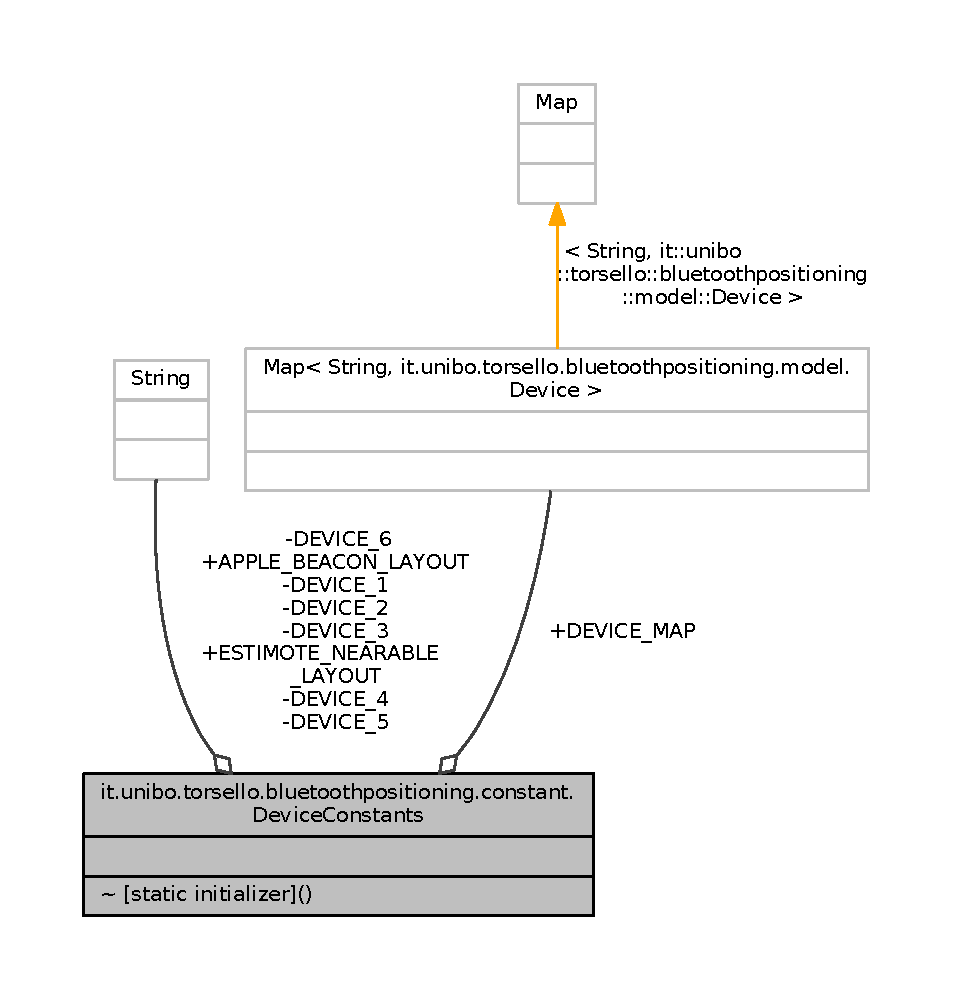
\includegraphics[width=350pt]{classit_1_1unibo_1_1torsello_1_1bluetoothpositioning_1_1constant_1_1DeviceConstants__coll__graph}
\end{center}
\end{figure}
\subsubsection*{Attributi pubblici statici}
\begin{DoxyCompactItemize}
\item 
static final String \hyperlink{classit_1_1unibo_1_1torsello_1_1bluetoothpositioning_1_1constant_1_1DeviceConstants_aceeec7a976dbf40e88728927bec61635_aceeec7a976dbf40e88728927bec61635}{A\+P\+P\+L\+E\+\_\+\+B\+E\+A\+C\+O\+N\+\_\+\+L\+A\+Y\+O\+UT} = \char`\"{}m\+:2-\/3=0215,i\+:4-\/19,i\+:20-\/21,i\+:22-\/23,p\+:24-\/24\char`\"{}
\item 
static final String \hyperlink{classit_1_1unibo_1_1torsello_1_1bluetoothpositioning_1_1constant_1_1DeviceConstants_ac80c3bbd15b47afacffefcdac59e7427_ac80c3bbd15b47afacffefcdac59e7427}{E\+S\+T\+I\+M\+O\+T\+E\+\_\+\+N\+E\+A\+R\+A\+B\+L\+E\+\_\+\+L\+A\+Y\+O\+UT}
\item 
static final Map$<$ String, \hyperlink{classit_1_1unibo_1_1torsello_1_1bluetoothpositioning_1_1model_1_1Device}{Device} $>$ \hyperlink{classit_1_1unibo_1_1torsello_1_1bluetoothpositioning_1_1constant_1_1DeviceConstants_adc3b2d4771c17a3ec55c070dfbe6151a_adc3b2d4771c17a3ec55c070dfbe6151a}{D\+E\+V\+I\+C\+E\+\_\+\+M\+AP}
\end{DoxyCompactItemize}
\subsubsection*{Funzioni statiche con visibilità di package}
\begin{DoxyCompactItemize}
\item 
\hyperlink{classit_1_1unibo_1_1torsello_1_1bluetoothpositioning_1_1constant_1_1DeviceConstants_a99a34b8f281a9d6229cf0adcdc9acd28_a99a34b8f281a9d6229cf0adcdc9acd28}{\mbox{[}static initializer\mbox{]}}
\end{DoxyCompactItemize}
\subsubsection*{Attributi privati statici}
\begin{DoxyCompactItemize}
\item 
static final String \hyperlink{classit_1_1unibo_1_1torsello_1_1bluetoothpositioning_1_1constant_1_1DeviceConstants_a1be810cb4e758baabfa5350f2185b4e1_a1be810cb4e758baabfa5350f2185b4e1}{D\+E\+V\+I\+C\+E\+\_\+1} = \char`\"{}C1\+:9\+B\+:\+B0\+:\+B9\+:01\+:9E\char`\"{}
\item 
static final String \hyperlink{classit_1_1unibo_1_1torsello_1_1bluetoothpositioning_1_1constant_1_1DeviceConstants_a6e71224c86695cf216855bc6c0c77a2d_a6e71224c86695cf216855bc6c0c77a2d}{D\+E\+V\+I\+C\+E\+\_\+2} = \char`\"{}D1\+:\+B\+E\+:\+E2\+:\+E9\+:67\+:\+A6\char`\"{}
\item 
static final String \hyperlink{classit_1_1unibo_1_1torsello_1_1bluetoothpositioning_1_1constant_1_1DeviceConstants_abfaa226793391615faf49ee223f594fb_abfaa226793391615faf49ee223f594fb}{D\+E\+V\+I\+C\+E\+\_\+3} = \char`\"{}F\+A\+:6\+B\+:72\+:1\+E\+:\+E\+B\+:46\char`\"{}
\item 
static final String \hyperlink{classit_1_1unibo_1_1torsello_1_1bluetoothpositioning_1_1constant_1_1DeviceConstants_a77b0930bc8fba094ecdbf42c91d707ea_a77b0930bc8fba094ecdbf42c91d707ea}{D\+E\+V\+I\+C\+E\+\_\+4} = \char`\"{}D9\+:80\+:00\+:\+B7\+:16\+:78\char`\"{}
\item 
static final String \hyperlink{classit_1_1unibo_1_1torsello_1_1bluetoothpositioning_1_1constant_1_1DeviceConstants_a89c9787da5f909162555b4ff956beae4_a89c9787da5f909162555b4ff956beae4}{D\+E\+V\+I\+C\+E\+\_\+5} = \char`\"{}D\+B\+:\+F6\+:\+F5\+:0\+C\+:23\+:\+BF\char`\"{}
\item 
static final String \hyperlink{classit_1_1unibo_1_1torsello_1_1bluetoothpositioning_1_1constant_1_1DeviceConstants_adcdd15d4bd91950603204b771d985527_adcdd15d4bd91950603204b771d985527}{D\+E\+V\+I\+C\+E\+\_\+6} = \char`\"{}E7\+:\+E4\+:0\+E\+:\+F6\+:79\+:3F\char`\"{}
\end{DoxyCompactItemize}


\subsubsection{Descrizione dettagliata}
Created by Federico Torsello. \href{mailto:federico.torsello@studio.unibo.it}{\tt federico.\+torsello@studio.\+unibo.\+it} 

\subsubsection{Documentazione delle funzioni membro}
\hypertarget{classit_1_1unibo_1_1torsello_1_1bluetoothpositioning_1_1constant_1_1DeviceConstants_a99a34b8f281a9d6229cf0adcdc9acd28_a99a34b8f281a9d6229cf0adcdc9acd28}{}\label{classit_1_1unibo_1_1torsello_1_1bluetoothpositioning_1_1constant_1_1DeviceConstants_a99a34b8f281a9d6229cf0adcdc9acd28_a99a34b8f281a9d6229cf0adcdc9acd28} 
\index{it\+::unibo\+::torsello\+::bluetoothpositioning\+::constant\+::\+Device\+Constants@{it\+::unibo\+::torsello\+::bluetoothpositioning\+::constant\+::\+Device\+Constants}!\mbox{[}static initializer\mbox{]}@{[static initializer]}}
\index{\mbox{[}static initializer\mbox{]}@{[static initializer]}!it\+::unibo\+::torsello\+::bluetoothpositioning\+::constant\+::\+Device\+Constants@{it\+::unibo\+::torsello\+::bluetoothpositioning\+::constant\+::\+Device\+Constants}}
\paragraph{\texorpdfstring{[static initializer]()}{[static initializer]()}}
{\footnotesize\ttfamily it.\+unibo.\+torsello.\+bluetoothpositioning.\+constant.\+Device\+Constants.\mbox{[}static initializer\mbox{]} (\begin{DoxyParamCaption}{ }\end{DoxyParamCaption})\hspace{0.3cm}{\ttfamily [static]}, {\ttfamily [package]}}



\subsubsection{Documentazione dei membri dato}
\hypertarget{classit_1_1unibo_1_1torsello_1_1bluetoothpositioning_1_1constant_1_1DeviceConstants_aceeec7a976dbf40e88728927bec61635_aceeec7a976dbf40e88728927bec61635}{}\label{classit_1_1unibo_1_1torsello_1_1bluetoothpositioning_1_1constant_1_1DeviceConstants_aceeec7a976dbf40e88728927bec61635_aceeec7a976dbf40e88728927bec61635} 
\index{it\+::unibo\+::torsello\+::bluetoothpositioning\+::constant\+::\+Device\+Constants@{it\+::unibo\+::torsello\+::bluetoothpositioning\+::constant\+::\+Device\+Constants}!A\+P\+P\+L\+E\+\_\+\+B\+E\+A\+C\+O\+N\+\_\+\+L\+A\+Y\+O\+UT@{A\+P\+P\+L\+E\+\_\+\+B\+E\+A\+C\+O\+N\+\_\+\+L\+A\+Y\+O\+UT}}
\index{A\+P\+P\+L\+E\+\_\+\+B\+E\+A\+C\+O\+N\+\_\+\+L\+A\+Y\+O\+UT@{A\+P\+P\+L\+E\+\_\+\+B\+E\+A\+C\+O\+N\+\_\+\+L\+A\+Y\+O\+UT}!it\+::unibo\+::torsello\+::bluetoothpositioning\+::constant\+::\+Device\+Constants@{it\+::unibo\+::torsello\+::bluetoothpositioning\+::constant\+::\+Device\+Constants}}
\paragraph{\texorpdfstring{A\+P\+P\+L\+E\+\_\+\+B\+E\+A\+C\+O\+N\+\_\+\+L\+A\+Y\+O\+UT}{APPLE\_BEACON\_LAYOUT}}
{\footnotesize\ttfamily final String it.\+unibo.\+torsello.\+bluetoothpositioning.\+constant.\+Device\+Constants.\+A\+P\+P\+L\+E\+\_\+\+B\+E\+A\+C\+O\+N\+\_\+\+L\+A\+Y\+O\+UT = \char`\"{}m\+:2-\/3=0215,i\+:4-\/19,i\+:20-\/21,i\+:22-\/23,p\+:24-\/24\char`\"{}\hspace{0.3cm}{\ttfamily [static]}}

\hypertarget{classit_1_1unibo_1_1torsello_1_1bluetoothpositioning_1_1constant_1_1DeviceConstants_a1be810cb4e758baabfa5350f2185b4e1_a1be810cb4e758baabfa5350f2185b4e1}{}\label{classit_1_1unibo_1_1torsello_1_1bluetoothpositioning_1_1constant_1_1DeviceConstants_a1be810cb4e758baabfa5350f2185b4e1_a1be810cb4e758baabfa5350f2185b4e1} 
\index{it\+::unibo\+::torsello\+::bluetoothpositioning\+::constant\+::\+Device\+Constants@{it\+::unibo\+::torsello\+::bluetoothpositioning\+::constant\+::\+Device\+Constants}!D\+E\+V\+I\+C\+E\+\_\+1@{D\+E\+V\+I\+C\+E\+\_\+1}}
\index{D\+E\+V\+I\+C\+E\+\_\+1@{D\+E\+V\+I\+C\+E\+\_\+1}!it\+::unibo\+::torsello\+::bluetoothpositioning\+::constant\+::\+Device\+Constants@{it\+::unibo\+::torsello\+::bluetoothpositioning\+::constant\+::\+Device\+Constants}}
\paragraph{\texorpdfstring{D\+E\+V\+I\+C\+E\+\_\+1}{DEVICE\_1}}
{\footnotesize\ttfamily final String it.\+unibo.\+torsello.\+bluetoothpositioning.\+constant.\+Device\+Constants.\+D\+E\+V\+I\+C\+E\+\_\+1 = \char`\"{}C1\+:9\+B\+:\+B0\+:\+B9\+:01\+:9E\char`\"{}\hspace{0.3cm}{\ttfamily [static]}, {\ttfamily [private]}}

\hypertarget{classit_1_1unibo_1_1torsello_1_1bluetoothpositioning_1_1constant_1_1DeviceConstants_a6e71224c86695cf216855bc6c0c77a2d_a6e71224c86695cf216855bc6c0c77a2d}{}\label{classit_1_1unibo_1_1torsello_1_1bluetoothpositioning_1_1constant_1_1DeviceConstants_a6e71224c86695cf216855bc6c0c77a2d_a6e71224c86695cf216855bc6c0c77a2d} 
\index{it\+::unibo\+::torsello\+::bluetoothpositioning\+::constant\+::\+Device\+Constants@{it\+::unibo\+::torsello\+::bluetoothpositioning\+::constant\+::\+Device\+Constants}!D\+E\+V\+I\+C\+E\+\_\+2@{D\+E\+V\+I\+C\+E\+\_\+2}}
\index{D\+E\+V\+I\+C\+E\+\_\+2@{D\+E\+V\+I\+C\+E\+\_\+2}!it\+::unibo\+::torsello\+::bluetoothpositioning\+::constant\+::\+Device\+Constants@{it\+::unibo\+::torsello\+::bluetoothpositioning\+::constant\+::\+Device\+Constants}}
\paragraph{\texorpdfstring{D\+E\+V\+I\+C\+E\+\_\+2}{DEVICE\_2}}
{\footnotesize\ttfamily final String it.\+unibo.\+torsello.\+bluetoothpositioning.\+constant.\+Device\+Constants.\+D\+E\+V\+I\+C\+E\+\_\+2 = \char`\"{}D1\+:\+B\+E\+:\+E2\+:\+E9\+:67\+:\+A6\char`\"{}\hspace{0.3cm}{\ttfamily [static]}, {\ttfamily [private]}}

\hypertarget{classit_1_1unibo_1_1torsello_1_1bluetoothpositioning_1_1constant_1_1DeviceConstants_abfaa226793391615faf49ee223f594fb_abfaa226793391615faf49ee223f594fb}{}\label{classit_1_1unibo_1_1torsello_1_1bluetoothpositioning_1_1constant_1_1DeviceConstants_abfaa226793391615faf49ee223f594fb_abfaa226793391615faf49ee223f594fb} 
\index{it\+::unibo\+::torsello\+::bluetoothpositioning\+::constant\+::\+Device\+Constants@{it\+::unibo\+::torsello\+::bluetoothpositioning\+::constant\+::\+Device\+Constants}!D\+E\+V\+I\+C\+E\+\_\+3@{D\+E\+V\+I\+C\+E\+\_\+3}}
\index{D\+E\+V\+I\+C\+E\+\_\+3@{D\+E\+V\+I\+C\+E\+\_\+3}!it\+::unibo\+::torsello\+::bluetoothpositioning\+::constant\+::\+Device\+Constants@{it\+::unibo\+::torsello\+::bluetoothpositioning\+::constant\+::\+Device\+Constants}}
\paragraph{\texorpdfstring{D\+E\+V\+I\+C\+E\+\_\+3}{DEVICE\_3}}
{\footnotesize\ttfamily final String it.\+unibo.\+torsello.\+bluetoothpositioning.\+constant.\+Device\+Constants.\+D\+E\+V\+I\+C\+E\+\_\+3 = \char`\"{}F\+A\+:6\+B\+:72\+:1\+E\+:\+E\+B\+:46\char`\"{}\hspace{0.3cm}{\ttfamily [static]}, {\ttfamily [private]}}

\hypertarget{classit_1_1unibo_1_1torsello_1_1bluetoothpositioning_1_1constant_1_1DeviceConstants_a77b0930bc8fba094ecdbf42c91d707ea_a77b0930bc8fba094ecdbf42c91d707ea}{}\label{classit_1_1unibo_1_1torsello_1_1bluetoothpositioning_1_1constant_1_1DeviceConstants_a77b0930bc8fba094ecdbf42c91d707ea_a77b0930bc8fba094ecdbf42c91d707ea} 
\index{it\+::unibo\+::torsello\+::bluetoothpositioning\+::constant\+::\+Device\+Constants@{it\+::unibo\+::torsello\+::bluetoothpositioning\+::constant\+::\+Device\+Constants}!D\+E\+V\+I\+C\+E\+\_\+4@{D\+E\+V\+I\+C\+E\+\_\+4}}
\index{D\+E\+V\+I\+C\+E\+\_\+4@{D\+E\+V\+I\+C\+E\+\_\+4}!it\+::unibo\+::torsello\+::bluetoothpositioning\+::constant\+::\+Device\+Constants@{it\+::unibo\+::torsello\+::bluetoothpositioning\+::constant\+::\+Device\+Constants}}
\paragraph{\texorpdfstring{D\+E\+V\+I\+C\+E\+\_\+4}{DEVICE\_4}}
{\footnotesize\ttfamily final String it.\+unibo.\+torsello.\+bluetoothpositioning.\+constant.\+Device\+Constants.\+D\+E\+V\+I\+C\+E\+\_\+4 = \char`\"{}D9\+:80\+:00\+:\+B7\+:16\+:78\char`\"{}\hspace{0.3cm}{\ttfamily [static]}, {\ttfamily [private]}}

\hypertarget{classit_1_1unibo_1_1torsello_1_1bluetoothpositioning_1_1constant_1_1DeviceConstants_a89c9787da5f909162555b4ff956beae4_a89c9787da5f909162555b4ff956beae4}{}\label{classit_1_1unibo_1_1torsello_1_1bluetoothpositioning_1_1constant_1_1DeviceConstants_a89c9787da5f909162555b4ff956beae4_a89c9787da5f909162555b4ff956beae4} 
\index{it\+::unibo\+::torsello\+::bluetoothpositioning\+::constant\+::\+Device\+Constants@{it\+::unibo\+::torsello\+::bluetoothpositioning\+::constant\+::\+Device\+Constants}!D\+E\+V\+I\+C\+E\+\_\+5@{D\+E\+V\+I\+C\+E\+\_\+5}}
\index{D\+E\+V\+I\+C\+E\+\_\+5@{D\+E\+V\+I\+C\+E\+\_\+5}!it\+::unibo\+::torsello\+::bluetoothpositioning\+::constant\+::\+Device\+Constants@{it\+::unibo\+::torsello\+::bluetoothpositioning\+::constant\+::\+Device\+Constants}}
\paragraph{\texorpdfstring{D\+E\+V\+I\+C\+E\+\_\+5}{DEVICE\_5}}
{\footnotesize\ttfamily final String it.\+unibo.\+torsello.\+bluetoothpositioning.\+constant.\+Device\+Constants.\+D\+E\+V\+I\+C\+E\+\_\+5 = \char`\"{}D\+B\+:\+F6\+:\+F5\+:0\+C\+:23\+:\+BF\char`\"{}\hspace{0.3cm}{\ttfamily [static]}, {\ttfamily [private]}}

\hypertarget{classit_1_1unibo_1_1torsello_1_1bluetoothpositioning_1_1constant_1_1DeviceConstants_adcdd15d4bd91950603204b771d985527_adcdd15d4bd91950603204b771d985527}{}\label{classit_1_1unibo_1_1torsello_1_1bluetoothpositioning_1_1constant_1_1DeviceConstants_adcdd15d4bd91950603204b771d985527_adcdd15d4bd91950603204b771d985527} 
\index{it\+::unibo\+::torsello\+::bluetoothpositioning\+::constant\+::\+Device\+Constants@{it\+::unibo\+::torsello\+::bluetoothpositioning\+::constant\+::\+Device\+Constants}!D\+E\+V\+I\+C\+E\+\_\+6@{D\+E\+V\+I\+C\+E\+\_\+6}}
\index{D\+E\+V\+I\+C\+E\+\_\+6@{D\+E\+V\+I\+C\+E\+\_\+6}!it\+::unibo\+::torsello\+::bluetoothpositioning\+::constant\+::\+Device\+Constants@{it\+::unibo\+::torsello\+::bluetoothpositioning\+::constant\+::\+Device\+Constants}}
\paragraph{\texorpdfstring{D\+E\+V\+I\+C\+E\+\_\+6}{DEVICE\_6}}
{\footnotesize\ttfamily final String it.\+unibo.\+torsello.\+bluetoothpositioning.\+constant.\+Device\+Constants.\+D\+E\+V\+I\+C\+E\+\_\+6 = \char`\"{}E7\+:\+E4\+:0\+E\+:\+F6\+:79\+:3F\char`\"{}\hspace{0.3cm}{\ttfamily [static]}, {\ttfamily [private]}}

\hypertarget{classit_1_1unibo_1_1torsello_1_1bluetoothpositioning_1_1constant_1_1DeviceConstants_adc3b2d4771c17a3ec55c070dfbe6151a_adc3b2d4771c17a3ec55c070dfbe6151a}{}\label{classit_1_1unibo_1_1torsello_1_1bluetoothpositioning_1_1constant_1_1DeviceConstants_adc3b2d4771c17a3ec55c070dfbe6151a_adc3b2d4771c17a3ec55c070dfbe6151a} 
\index{it\+::unibo\+::torsello\+::bluetoothpositioning\+::constant\+::\+Device\+Constants@{it\+::unibo\+::torsello\+::bluetoothpositioning\+::constant\+::\+Device\+Constants}!D\+E\+V\+I\+C\+E\+\_\+\+M\+AP@{D\+E\+V\+I\+C\+E\+\_\+\+M\+AP}}
\index{D\+E\+V\+I\+C\+E\+\_\+\+M\+AP@{D\+E\+V\+I\+C\+E\+\_\+\+M\+AP}!it\+::unibo\+::torsello\+::bluetoothpositioning\+::constant\+::\+Device\+Constants@{it\+::unibo\+::torsello\+::bluetoothpositioning\+::constant\+::\+Device\+Constants}}
\paragraph{\texorpdfstring{D\+E\+V\+I\+C\+E\+\_\+\+M\+AP}{DEVICE\_MAP}}
{\footnotesize\ttfamily final Map$<$String, \hyperlink{classit_1_1unibo_1_1torsello_1_1bluetoothpositioning_1_1model_1_1Device}{Device}$>$ it.\+unibo.\+torsello.\+bluetoothpositioning.\+constant.\+Device\+Constants.\+D\+E\+V\+I\+C\+E\+\_\+\+M\+AP\hspace{0.3cm}{\ttfamily [static]}}

\hypertarget{classit_1_1unibo_1_1torsello_1_1bluetoothpositioning_1_1constant_1_1DeviceConstants_ac80c3bbd15b47afacffefcdac59e7427_ac80c3bbd15b47afacffefcdac59e7427}{}\label{classit_1_1unibo_1_1torsello_1_1bluetoothpositioning_1_1constant_1_1DeviceConstants_ac80c3bbd15b47afacffefcdac59e7427_ac80c3bbd15b47afacffefcdac59e7427} 
\index{it\+::unibo\+::torsello\+::bluetoothpositioning\+::constant\+::\+Device\+Constants@{it\+::unibo\+::torsello\+::bluetoothpositioning\+::constant\+::\+Device\+Constants}!E\+S\+T\+I\+M\+O\+T\+E\+\_\+\+N\+E\+A\+R\+A\+B\+L\+E\+\_\+\+L\+A\+Y\+O\+UT@{E\+S\+T\+I\+M\+O\+T\+E\+\_\+\+N\+E\+A\+R\+A\+B\+L\+E\+\_\+\+L\+A\+Y\+O\+UT}}
\index{E\+S\+T\+I\+M\+O\+T\+E\+\_\+\+N\+E\+A\+R\+A\+B\+L\+E\+\_\+\+L\+A\+Y\+O\+UT@{E\+S\+T\+I\+M\+O\+T\+E\+\_\+\+N\+E\+A\+R\+A\+B\+L\+E\+\_\+\+L\+A\+Y\+O\+UT}!it\+::unibo\+::torsello\+::bluetoothpositioning\+::constant\+::\+Device\+Constants@{it\+::unibo\+::torsello\+::bluetoothpositioning\+::constant\+::\+Device\+Constants}}
\paragraph{\texorpdfstring{E\+S\+T\+I\+M\+O\+T\+E\+\_\+\+N\+E\+A\+R\+A\+B\+L\+E\+\_\+\+L\+A\+Y\+O\+UT}{ESTIMOTE\_NEARABLE\_LAYOUT}}
{\footnotesize\ttfamily final String it.\+unibo.\+torsello.\+bluetoothpositioning.\+constant.\+Device\+Constants.\+E\+S\+T\+I\+M\+O\+T\+E\+\_\+\+N\+E\+A\+R\+A\+B\+L\+E\+\_\+\+L\+A\+Y\+O\+UT\hspace{0.3cm}{\ttfamily [static]}}

{\bfseries Valore iniziale\+:}
\begin{DoxyCode}
= \textcolor{stringliteral}{"m:1-2=0101,i:3-10,d:11-11,d:12-12,"} +
            \textcolor{stringliteral}{"d:13-14,d:15-15,d:16-16,d:17-17,d:18-18,d:19-19,d:20-20, p:21-21"}
\end{DoxyCode}


La documentazione per questa classe è stata generata a partire dal seguente file\+:\begin{DoxyCompactItemize}
\item 
\hyperlink{DeviceConstants_8java}{Device\+Constants.\+java}\end{DoxyCompactItemize}

\hypertarget{classit_1_1unibo_1_1torsello_1_1bluetoothpositioning_1_1fragment_1_1DeviceDetailFragment}{}\subsection{Riferimenti per la classe it.\+unibo.\+torsello.\+bluetoothpositioning.\+fragment.\+Device\+Detail\+Fragment}
\label{classit_1_1unibo_1_1torsello_1_1bluetoothpositioning_1_1fragment_1_1DeviceDetailFragment}\index{it.\+unibo.\+torsello.\+bluetoothpositioning.\+fragment.\+Device\+Detail\+Fragment@{it.\+unibo.\+torsello.\+bluetoothpositioning.\+fragment.\+Device\+Detail\+Fragment}}


Diagramma delle classi per it.\+unibo.\+torsello.\+bluetoothpositioning.\+fragment.\+Device\+Detail\+Fragment
\nopagebreak
\begin{figure}[H]
\begin{center}
\leavevmode
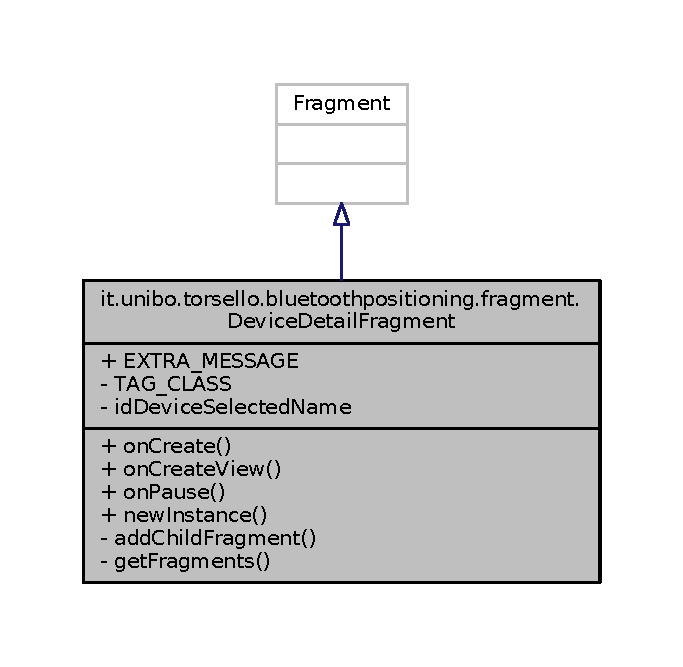
\includegraphics[width=328pt]{classit_1_1unibo_1_1torsello_1_1bluetoothpositioning_1_1fragment_1_1DeviceDetailFragment__inherit__graph}
\end{center}
\end{figure}


Diagramma di collaborazione per it.\+unibo.\+torsello.\+bluetoothpositioning.\+fragment.\+Device\+Detail\+Fragment\+:
\nopagebreak
\begin{figure}[H]
\begin{center}
\leavevmode
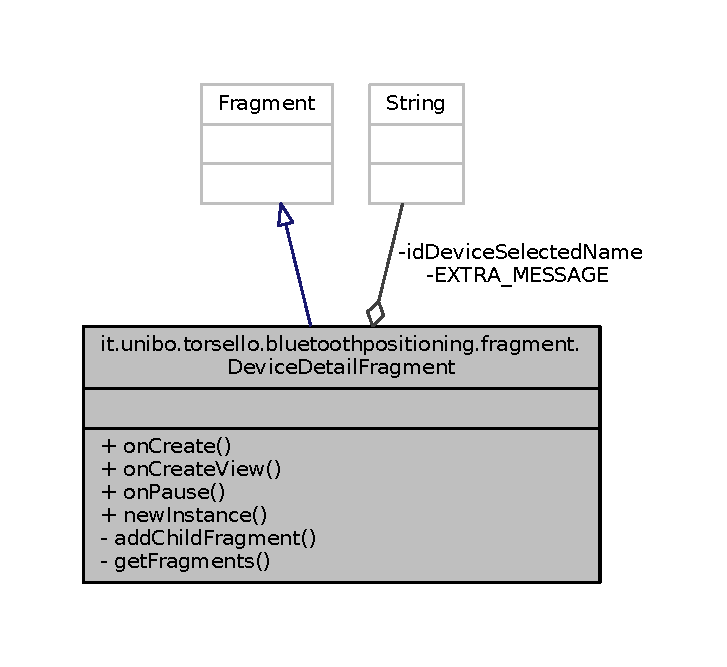
\includegraphics[width=349pt]{classit_1_1unibo_1_1torsello_1_1bluetoothpositioning_1_1fragment_1_1DeviceDetailFragment__coll__graph}
\end{center}
\end{figure}
\subsubsection*{Membri pubblici}
\begin{DoxyCompactItemize}
\item 
void \hyperlink{classit_1_1unibo_1_1torsello_1_1bluetoothpositioning_1_1fragment_1_1DeviceDetailFragment_af33d782c107be10fe752f16f04cc5e5d_af33d782c107be10fe752f16f04cc5e5d}{on\+Create} (Bundle saved\+Instance\+State)
\item 
View \hyperlink{classit_1_1unibo_1_1torsello_1_1bluetoothpositioning_1_1fragment_1_1DeviceDetailFragment_a6d43be281b577e0d9f2540fea30c2fdf_a6d43be281b577e0d9f2540fea30c2fdf}{on\+Create\+View} (Layout\+Inflater inflater, View\+Group container, Bundle saved\+Instance\+State)
\item 
void \hyperlink{classit_1_1unibo_1_1torsello_1_1bluetoothpositioning_1_1fragment_1_1DeviceDetailFragment_a1ed4762356dd3067ce48aa73da50404e_a1ed4762356dd3067ce48aa73da50404e}{on\+Pause} ()
\end{DoxyCompactItemize}
\subsubsection*{Membri pubblici statici}
\begin{DoxyCompactItemize}
\item 
static \hyperlink{classit_1_1unibo_1_1torsello_1_1bluetoothpositioning_1_1fragment_1_1DeviceDetailFragment}{Device\+Detail\+Fragment} \hyperlink{classit_1_1unibo_1_1torsello_1_1bluetoothpositioning_1_1fragment_1_1DeviceDetailFragment_a626de18d36d44ae0b4ff21c2527bdf5a_a626de18d36d44ae0b4ff21c2527bdf5a}{new\+Instance} (String message)
\end{DoxyCompactItemize}
\subsubsection*{Membri privati}
\begin{DoxyCompactItemize}
\item 
void \hyperlink{classit_1_1unibo_1_1torsello_1_1bluetoothpositioning_1_1fragment_1_1DeviceDetailFragment_a62c541b8382a522f06a5d9c56cf50b26_a62c541b8382a522f06a5d9c56cf50b26}{add\+Child\+Fragment} (View root)
\item 
Array\+List$<$ Fragment $>$ \hyperlink{classit_1_1unibo_1_1torsello_1_1bluetoothpositioning_1_1fragment_1_1DeviceDetailFragment_a98e370cfcbfe5eaa4e1fe9242b00e639_a98e370cfcbfe5eaa4e1fe9242b00e639}{get\+Fragments} ()
\end{DoxyCompactItemize}
\subsubsection*{Attributi privati}
\begin{DoxyCompactItemize}
\item 
String \hyperlink{classit_1_1unibo_1_1torsello_1_1bluetoothpositioning_1_1fragment_1_1DeviceDetailFragment_a6d52d8371a07fb8da75879758d1d6942_a6d52d8371a07fb8da75879758d1d6942}{id\+Device\+Selected\+Name}
\end{DoxyCompactItemize}
\subsubsection*{Attributi privati statici}
\begin{DoxyCompactItemize}
\item 
static final String \hyperlink{classit_1_1unibo_1_1torsello_1_1bluetoothpositioning_1_1fragment_1_1DeviceDetailFragment_a9f7fff4a2b22105976f2c7223d88f9ae_a9f7fff4a2b22105976f2c7223d88f9ae}{E\+X\+T\+R\+A\+\_\+\+M\+E\+S\+S\+A\+GE} = \char`\"{}E\+X\+T\+R\+A\+\_\+\+M\+E\+S\+S\+A\+GE\char`\"{}
\end{DoxyCompactItemize}


\subsubsection{Descrizione dettagliata}
Created by Federico Torsello. \href{mailto:federico.torsello@studio.unibo.it}{\tt federico.\+torsello@studio.\+unibo.\+it} 

\subsubsection{Documentazione delle funzioni membro}
\hypertarget{classit_1_1unibo_1_1torsello_1_1bluetoothpositioning_1_1fragment_1_1DeviceDetailFragment_a62c541b8382a522f06a5d9c56cf50b26_a62c541b8382a522f06a5d9c56cf50b26}{}\label{classit_1_1unibo_1_1torsello_1_1bluetoothpositioning_1_1fragment_1_1DeviceDetailFragment_a62c541b8382a522f06a5d9c56cf50b26_a62c541b8382a522f06a5d9c56cf50b26} 
\index{it\+::unibo\+::torsello\+::bluetoothpositioning\+::fragment\+::\+Device\+Detail\+Fragment@{it\+::unibo\+::torsello\+::bluetoothpositioning\+::fragment\+::\+Device\+Detail\+Fragment}!add\+Child\+Fragment@{add\+Child\+Fragment}}
\index{add\+Child\+Fragment@{add\+Child\+Fragment}!it\+::unibo\+::torsello\+::bluetoothpositioning\+::fragment\+::\+Device\+Detail\+Fragment@{it\+::unibo\+::torsello\+::bluetoothpositioning\+::fragment\+::\+Device\+Detail\+Fragment}}
\paragraph{\texorpdfstring{add\+Child\+Fragment()}{addChildFragment()}}
{\footnotesize\ttfamily void it.\+unibo.\+torsello.\+bluetoothpositioning.\+fragment.\+Device\+Detail\+Fragment.\+add\+Child\+Fragment (\begin{DoxyParamCaption}\item[{View}]{root }\end{DoxyParamCaption})\hspace{0.3cm}{\ttfamily [private]}}


\begin{DoxyCode}
63                                              \{
64 
65         ViewPager mViewPager = (ViewPager) root.findViewById(R.id.view\_pager);
66         StatePagerAdapter myPageAdapter = \textcolor{keyword}{new} StatePagerAdapter(getChildFragmentManager(), 
      \hyperlink{classit_1_1unibo_1_1torsello_1_1bluetoothpositioning_1_1fragment_1_1DeviceDetailFragment_a98e370cfcbfe5eaa4e1fe9242b00e639_a98e370cfcbfe5eaa4e1fe9242b00e639}{getFragments}());
67         mViewPager.setAdapter(myPageAdapter);
68 
69         TabLayout tabLayout = (TabLayout) root.findViewById(R.id.sliding\_tabs);
70         tabLayout.setupWithViewPager(mViewPager);
71     \}
\end{DoxyCode}
\hypertarget{classit_1_1unibo_1_1torsello_1_1bluetoothpositioning_1_1fragment_1_1DeviceDetailFragment_a98e370cfcbfe5eaa4e1fe9242b00e639_a98e370cfcbfe5eaa4e1fe9242b00e639}{}\label{classit_1_1unibo_1_1torsello_1_1bluetoothpositioning_1_1fragment_1_1DeviceDetailFragment_a98e370cfcbfe5eaa4e1fe9242b00e639_a98e370cfcbfe5eaa4e1fe9242b00e639} 
\index{it\+::unibo\+::torsello\+::bluetoothpositioning\+::fragment\+::\+Device\+Detail\+Fragment@{it\+::unibo\+::torsello\+::bluetoothpositioning\+::fragment\+::\+Device\+Detail\+Fragment}!get\+Fragments@{get\+Fragments}}
\index{get\+Fragments@{get\+Fragments}!it\+::unibo\+::torsello\+::bluetoothpositioning\+::fragment\+::\+Device\+Detail\+Fragment@{it\+::unibo\+::torsello\+::bluetoothpositioning\+::fragment\+::\+Device\+Detail\+Fragment}}
\paragraph{\texorpdfstring{get\+Fragments()}{getFragments()}}
{\footnotesize\ttfamily Array\+List$<$Fragment$>$ it.\+unibo.\+torsello.\+bluetoothpositioning.\+fragment.\+Device\+Detail\+Fragment.\+get\+Fragments (\begin{DoxyParamCaption}{ }\end{DoxyParamCaption})\hspace{0.3cm}{\ttfamily [private]}}


\begin{DoxyCode}
73                                                \{
74 
75         ArrayList<Fragment> fragments = \textcolor{keyword}{new} ArrayList<>();
76 
77         \textcolor{comment}{// fragment 0}
78         fragments.add(DeviceDetailInner1Fragment.newInstance(
      \hyperlink{classit_1_1unibo_1_1torsello_1_1bluetoothpositioning_1_1fragment_1_1DeviceDetailFragment_a6d52d8371a07fb8da75879758d1d6942_a6d52d8371a07fb8da75879758d1d6942}{idDeviceSelectedName}));
79 
80         \textcolor{comment}{// fragment 1}
81         fragments.add(DeviceDetailInner2Fragment.newInstance(\textcolor{stringliteral}{"Details"}, 
      \hyperlink{classit_1_1unibo_1_1torsello_1_1bluetoothpositioning_1_1fragment_1_1DeviceDetailFragment_a6d52d8371a07fb8da75879758d1d6942_a6d52d8371a07fb8da75879758d1d6942}{idDeviceSelectedName}));
82 
83 
84         \textcolor{keywordflow}{return} fragments;
85     \}
\end{DoxyCode}
\hypertarget{classit_1_1unibo_1_1torsello_1_1bluetoothpositioning_1_1fragment_1_1DeviceDetailFragment_a626de18d36d44ae0b4ff21c2527bdf5a_a626de18d36d44ae0b4ff21c2527bdf5a}{}\label{classit_1_1unibo_1_1torsello_1_1bluetoothpositioning_1_1fragment_1_1DeviceDetailFragment_a626de18d36d44ae0b4ff21c2527bdf5a_a626de18d36d44ae0b4ff21c2527bdf5a} 
\index{it\+::unibo\+::torsello\+::bluetoothpositioning\+::fragment\+::\+Device\+Detail\+Fragment@{it\+::unibo\+::torsello\+::bluetoothpositioning\+::fragment\+::\+Device\+Detail\+Fragment}!new\+Instance@{new\+Instance}}
\index{new\+Instance@{new\+Instance}!it\+::unibo\+::torsello\+::bluetoothpositioning\+::fragment\+::\+Device\+Detail\+Fragment@{it\+::unibo\+::torsello\+::bluetoothpositioning\+::fragment\+::\+Device\+Detail\+Fragment}}
\paragraph{\texorpdfstring{new\+Instance()}{newInstance()}}
{\footnotesize\ttfamily static \hyperlink{classit_1_1unibo_1_1torsello_1_1bluetoothpositioning_1_1fragment_1_1DeviceDetailFragment}{Device\+Detail\+Fragment} it.\+unibo.\+torsello.\+bluetoothpositioning.\+fragment.\+Device\+Detail\+Fragment.\+new\+Instance (\begin{DoxyParamCaption}\item[{String}]{message }\end{DoxyParamCaption})\hspace{0.3cm}{\ttfamily [static]}}


\begin{DoxyCode}
29                                                                    \{
30         DeviceDetailFragment fragment = \textcolor{keyword}{new} DeviceDetailFragment();
31         Bundle args = \textcolor{keyword}{new} Bundle();
32         args.putString(\hyperlink{classit_1_1unibo_1_1torsello_1_1bluetoothpositioning_1_1fragment_1_1DeviceDetailFragment_a9f7fff4a2b22105976f2c7223d88f9ae_a9f7fff4a2b22105976f2c7223d88f9ae}{EXTRA\_MESSAGE}, message);
33         fragment.setArguments(args);
34         \textcolor{keywordflow}{return} fragment;
35     \}
\end{DoxyCode}
\hypertarget{classit_1_1unibo_1_1torsello_1_1bluetoothpositioning_1_1fragment_1_1DeviceDetailFragment_af33d782c107be10fe752f16f04cc5e5d_af33d782c107be10fe752f16f04cc5e5d}{}\label{classit_1_1unibo_1_1torsello_1_1bluetoothpositioning_1_1fragment_1_1DeviceDetailFragment_af33d782c107be10fe752f16f04cc5e5d_af33d782c107be10fe752f16f04cc5e5d} 
\index{it\+::unibo\+::torsello\+::bluetoothpositioning\+::fragment\+::\+Device\+Detail\+Fragment@{it\+::unibo\+::torsello\+::bluetoothpositioning\+::fragment\+::\+Device\+Detail\+Fragment}!on\+Create@{on\+Create}}
\index{on\+Create@{on\+Create}!it\+::unibo\+::torsello\+::bluetoothpositioning\+::fragment\+::\+Device\+Detail\+Fragment@{it\+::unibo\+::torsello\+::bluetoothpositioning\+::fragment\+::\+Device\+Detail\+Fragment}}
\paragraph{\texorpdfstring{on\+Create()}{onCreate()}}
{\footnotesize\ttfamily void it.\+unibo.\+torsello.\+bluetoothpositioning.\+fragment.\+Device\+Detail\+Fragment.\+on\+Create (\begin{DoxyParamCaption}\item[{Bundle}]{saved\+Instance\+State }\end{DoxyParamCaption})}


\begin{DoxyCode}
38                                                     \{
39         super.onCreate(savedInstanceState);
40 
41         \hyperlink{classit_1_1unibo_1_1torsello_1_1bluetoothpositioning_1_1fragment_1_1DeviceDetailFragment_a6d52d8371a07fb8da75879758d1d6942_a6d52d8371a07fb8da75879758d1d6942}{idDeviceSelectedName} = getArguments().getString(
      \hyperlink{classit_1_1unibo_1_1torsello_1_1bluetoothpositioning_1_1fragment_1_1DeviceDetailFragment_a9f7fff4a2b22105976f2c7223d88f9ae_a9f7fff4a2b22105976f2c7223d88f9ae}{EXTRA\_MESSAGE});
42     \}
\end{DoxyCode}
\hypertarget{classit_1_1unibo_1_1torsello_1_1bluetoothpositioning_1_1fragment_1_1DeviceDetailFragment_a6d43be281b577e0d9f2540fea30c2fdf_a6d43be281b577e0d9f2540fea30c2fdf}{}\label{classit_1_1unibo_1_1torsello_1_1bluetoothpositioning_1_1fragment_1_1DeviceDetailFragment_a6d43be281b577e0d9f2540fea30c2fdf_a6d43be281b577e0d9f2540fea30c2fdf} 
\index{it\+::unibo\+::torsello\+::bluetoothpositioning\+::fragment\+::\+Device\+Detail\+Fragment@{it\+::unibo\+::torsello\+::bluetoothpositioning\+::fragment\+::\+Device\+Detail\+Fragment}!on\+Create\+View@{on\+Create\+View}}
\index{on\+Create\+View@{on\+Create\+View}!it\+::unibo\+::torsello\+::bluetoothpositioning\+::fragment\+::\+Device\+Detail\+Fragment@{it\+::unibo\+::torsello\+::bluetoothpositioning\+::fragment\+::\+Device\+Detail\+Fragment}}
\paragraph{\texorpdfstring{on\+Create\+View()}{onCreateView()}}
{\footnotesize\ttfamily View it.\+unibo.\+torsello.\+bluetoothpositioning.\+fragment.\+Device\+Detail\+Fragment.\+on\+Create\+View (\begin{DoxyParamCaption}\item[{Layout\+Inflater}]{inflater,  }\item[{View\+Group}]{container,  }\item[{Bundle}]{saved\+Instance\+State }\end{DoxyParamCaption})}


\begin{DoxyCode}
45                                                                                                       \{
46         \textcolor{keyword}{final} View root = inflater.inflate(R.layout.fragment\_device\_detail, container, \textcolor{keyword}{false});
47 
48         getActivity().findViewById(R.id.toolbar).setVisibility(View.GONE);
49 
50         ((AppBarLayout) root.findViewById(R.id.appbar\_detail)).setExpanded(\textcolor{keyword}{false});
51         ((CollapsingToolbarLayout) root.findViewById(R.id.collapsing\_toolbar)).setTitle(
      \hyperlink{classit_1_1unibo_1_1torsello_1_1bluetoothpositioning_1_1fragment_1_1DeviceDetailFragment_a6d52d8371a07fb8da75879758d1d6942_a6d52d8371a07fb8da75879758d1d6942}{idDeviceSelectedName});
52 
53         \hyperlink{classit_1_1unibo_1_1torsello_1_1bluetoothpositioning_1_1fragment_1_1DeviceDetailFragment_a62c541b8382a522f06a5d9c56cf50b26_a62c541b8382a522f06a5d9c56cf50b26}{addChildFragment}(root);
54         \textcolor{keywordflow}{return} root;
55     \}
\end{DoxyCode}
\hypertarget{classit_1_1unibo_1_1torsello_1_1bluetoothpositioning_1_1fragment_1_1DeviceDetailFragment_a1ed4762356dd3067ce48aa73da50404e_a1ed4762356dd3067ce48aa73da50404e}{}\label{classit_1_1unibo_1_1torsello_1_1bluetoothpositioning_1_1fragment_1_1DeviceDetailFragment_a1ed4762356dd3067ce48aa73da50404e_a1ed4762356dd3067ce48aa73da50404e} 
\index{it\+::unibo\+::torsello\+::bluetoothpositioning\+::fragment\+::\+Device\+Detail\+Fragment@{it\+::unibo\+::torsello\+::bluetoothpositioning\+::fragment\+::\+Device\+Detail\+Fragment}!on\+Pause@{on\+Pause}}
\index{on\+Pause@{on\+Pause}!it\+::unibo\+::torsello\+::bluetoothpositioning\+::fragment\+::\+Device\+Detail\+Fragment@{it\+::unibo\+::torsello\+::bluetoothpositioning\+::fragment\+::\+Device\+Detail\+Fragment}}
\paragraph{\texorpdfstring{on\+Pause()}{onPause()}}
{\footnotesize\ttfamily void it.\+unibo.\+torsello.\+bluetoothpositioning.\+fragment.\+Device\+Detail\+Fragment.\+on\+Pause (\begin{DoxyParamCaption}{ }\end{DoxyParamCaption})}


\begin{DoxyCode}
58                           \{
59         getActivity().findViewById(R.id.toolbar).setVisibility(View.VISIBLE);
60         super.onPause();
61     \}
\end{DoxyCode}


\subsubsection{Documentazione dei membri dato}
\hypertarget{classit_1_1unibo_1_1torsello_1_1bluetoothpositioning_1_1fragment_1_1DeviceDetailFragment_a9f7fff4a2b22105976f2c7223d88f9ae_a9f7fff4a2b22105976f2c7223d88f9ae}{}\label{classit_1_1unibo_1_1torsello_1_1bluetoothpositioning_1_1fragment_1_1DeviceDetailFragment_a9f7fff4a2b22105976f2c7223d88f9ae_a9f7fff4a2b22105976f2c7223d88f9ae} 
\index{it\+::unibo\+::torsello\+::bluetoothpositioning\+::fragment\+::\+Device\+Detail\+Fragment@{it\+::unibo\+::torsello\+::bluetoothpositioning\+::fragment\+::\+Device\+Detail\+Fragment}!E\+X\+T\+R\+A\+\_\+\+M\+E\+S\+S\+A\+GE@{E\+X\+T\+R\+A\+\_\+\+M\+E\+S\+S\+A\+GE}}
\index{E\+X\+T\+R\+A\+\_\+\+M\+E\+S\+S\+A\+GE@{E\+X\+T\+R\+A\+\_\+\+M\+E\+S\+S\+A\+GE}!it\+::unibo\+::torsello\+::bluetoothpositioning\+::fragment\+::\+Device\+Detail\+Fragment@{it\+::unibo\+::torsello\+::bluetoothpositioning\+::fragment\+::\+Device\+Detail\+Fragment}}
\paragraph{\texorpdfstring{E\+X\+T\+R\+A\+\_\+\+M\+E\+S\+S\+A\+GE}{EXTRA\_MESSAGE}}
{\footnotesize\ttfamily final String it.\+unibo.\+torsello.\+bluetoothpositioning.\+fragment.\+Device\+Detail\+Fragment.\+E\+X\+T\+R\+A\+\_\+\+M\+E\+S\+S\+A\+GE = \char`\"{}E\+X\+T\+R\+A\+\_\+\+M\+E\+S\+S\+A\+GE\char`\"{}\hspace{0.3cm}{\ttfamily [static]}, {\ttfamily [private]}}

\hypertarget{classit_1_1unibo_1_1torsello_1_1bluetoothpositioning_1_1fragment_1_1DeviceDetailFragment_a6d52d8371a07fb8da75879758d1d6942_a6d52d8371a07fb8da75879758d1d6942}{}\label{classit_1_1unibo_1_1torsello_1_1bluetoothpositioning_1_1fragment_1_1DeviceDetailFragment_a6d52d8371a07fb8da75879758d1d6942_a6d52d8371a07fb8da75879758d1d6942} 
\index{it\+::unibo\+::torsello\+::bluetoothpositioning\+::fragment\+::\+Device\+Detail\+Fragment@{it\+::unibo\+::torsello\+::bluetoothpositioning\+::fragment\+::\+Device\+Detail\+Fragment}!id\+Device\+Selected\+Name@{id\+Device\+Selected\+Name}}
\index{id\+Device\+Selected\+Name@{id\+Device\+Selected\+Name}!it\+::unibo\+::torsello\+::bluetoothpositioning\+::fragment\+::\+Device\+Detail\+Fragment@{it\+::unibo\+::torsello\+::bluetoothpositioning\+::fragment\+::\+Device\+Detail\+Fragment}}
\paragraph{\texorpdfstring{id\+Device\+Selected\+Name}{idDeviceSelectedName}}
{\footnotesize\ttfamily String it.\+unibo.\+torsello.\+bluetoothpositioning.\+fragment.\+Device\+Detail\+Fragment.\+id\+Device\+Selected\+Name\hspace{0.3cm}{\ttfamily [private]}}



La documentazione per questa classe è stata generata a partire dal seguente file\+:\begin{DoxyCompactItemize}
\item 
\hyperlink{DeviceDetailFragment_8java}{Device\+Detail\+Fragment.\+java}\end{DoxyCompactItemize}

\hypertarget{classit_1_1unibo_1_1torsello_1_1bluetoothpositioning_1_1fragment_1_1devicesObservers_1_1DeviceDetailInner1Fragment}{}\subsection{Riferimenti per la classe it.\+unibo.\+torsello.\+bluetoothpositioning.\+fragment.\+devices\+Observers.\+Device\+Detail\+Inner1\+Fragment}
\label{classit_1_1unibo_1_1torsello_1_1bluetoothpositioning_1_1fragment_1_1devicesObservers_1_1DeviceDetailInner1Fragment}\index{it.\+unibo.\+torsello.\+bluetoothpositioning.\+fragment.\+devices\+Observers.\+Device\+Detail\+Inner1\+Fragment@{it.\+unibo.\+torsello.\+bluetoothpositioning.\+fragment.\+devices\+Observers.\+Device\+Detail\+Inner1\+Fragment}}


Diagramma delle classi per it.\+unibo.\+torsello.\+bluetoothpositioning.\+fragment.\+devices\+Observers.\+Device\+Detail\+Inner1\+Fragment
\nopagebreak
\begin{figure}[H]
\begin{center}
\leavevmode
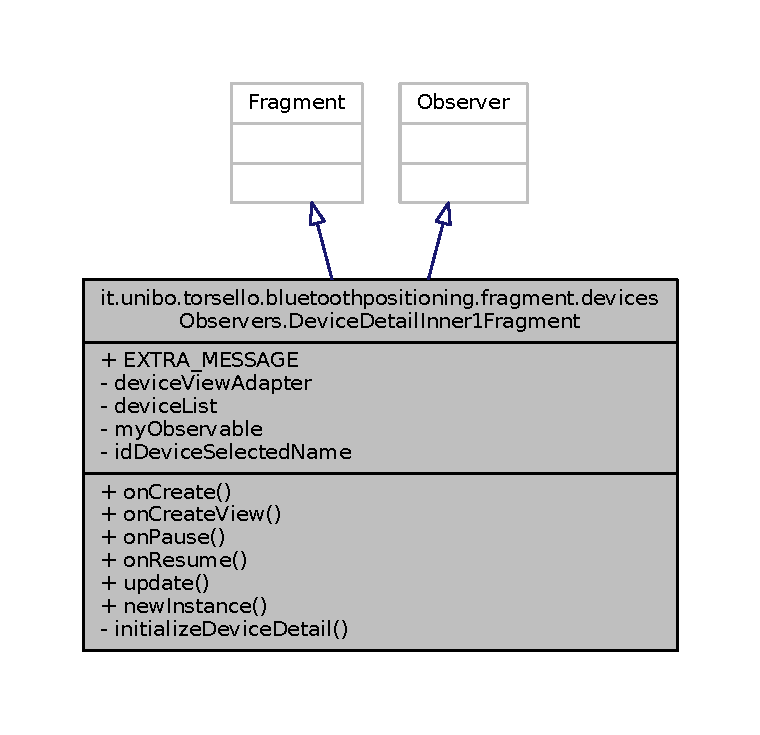
\includegraphics[width=350pt]{classit_1_1unibo_1_1torsello_1_1bluetoothpositioning_1_1fragment_1_1devicesObservers_1_1DeviceDe8362efa0b556f228cc3338a27b7e447c}
\end{center}
\end{figure}


Diagramma di collaborazione per it.\+unibo.\+torsello.\+bluetoothpositioning.\+fragment.\+devices\+Observers.\+Device\+Detail\+Inner1\+Fragment\+:
\nopagebreak
\begin{figure}[H]
\begin{center}
\leavevmode
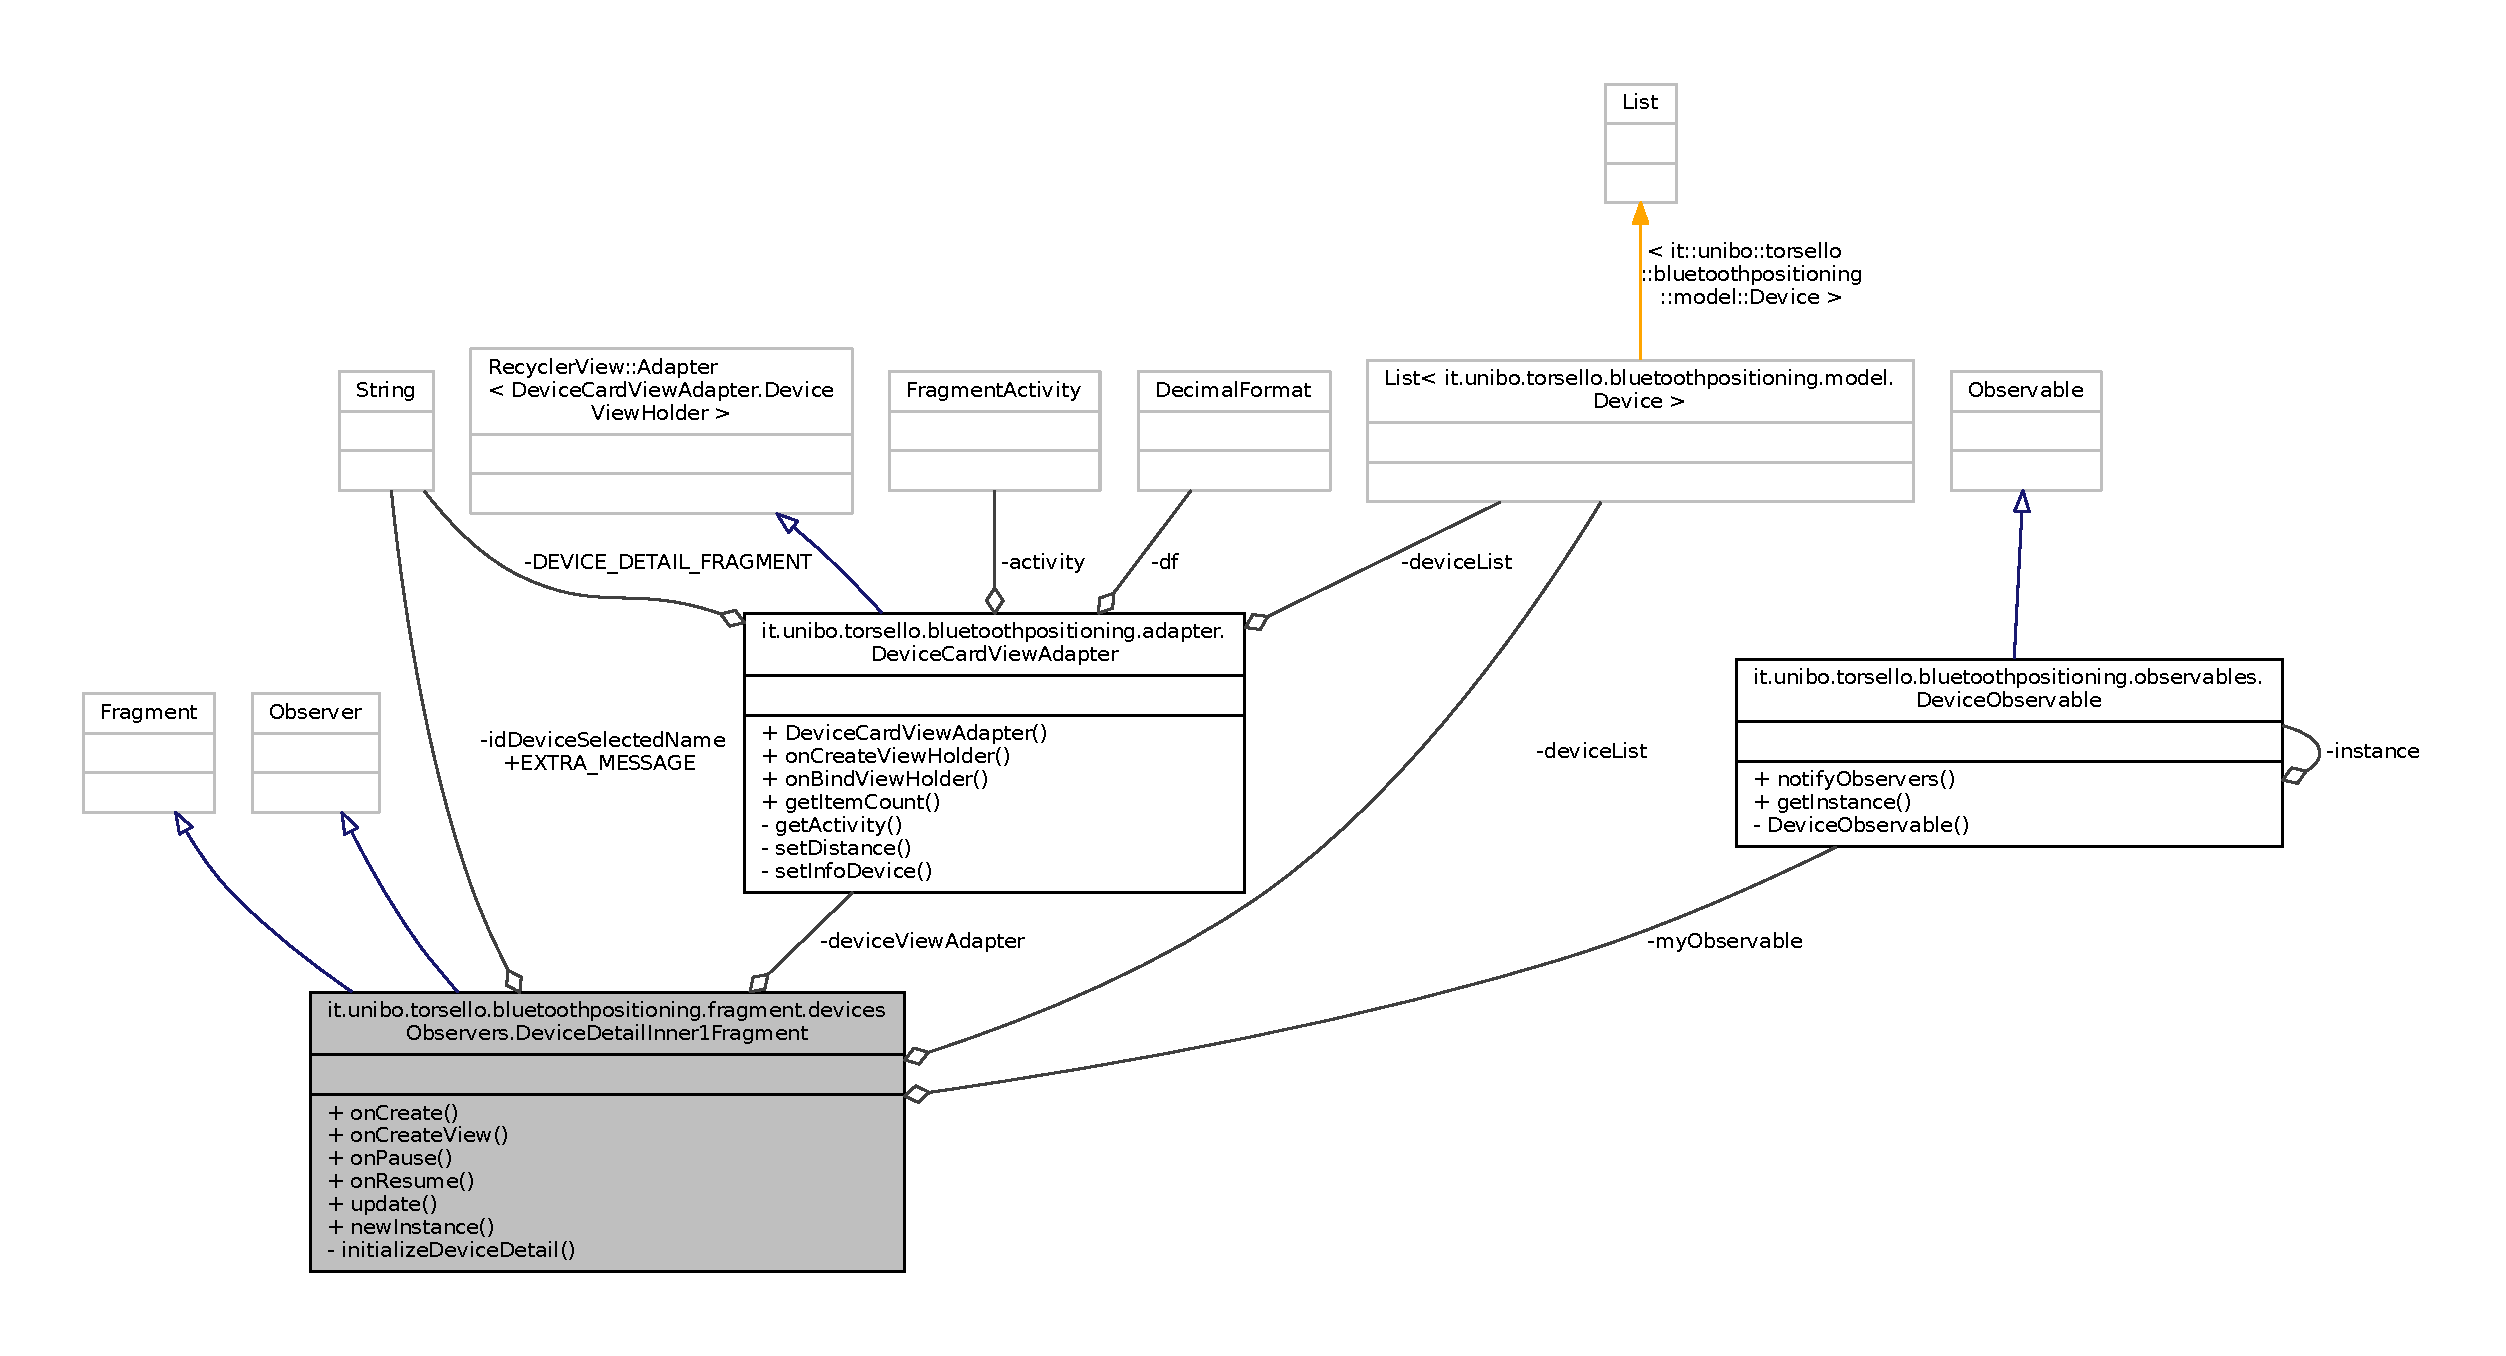
\includegraphics[width=350pt]{classit_1_1unibo_1_1torsello_1_1bluetoothpositioning_1_1fragment_1_1devicesObservers_1_1DeviceDetailInner1Fragment__coll__graph}
\end{center}
\end{figure}
\subsubsection*{Membri pubblici}
\begin{DoxyCompactItemize}
\item 
void \hyperlink{classit_1_1unibo_1_1torsello_1_1bluetoothpositioning_1_1fragment_1_1devicesObservers_1_1DeviceDetailInner1Fragment_aa2c5b397a4773bcd426c4ce3f5e291b4_aa2c5b397a4773bcd426c4ce3f5e291b4}{on\+Create} (@Nullable Bundle saved\+Instance\+State)
\item 
View \hyperlink{classit_1_1unibo_1_1torsello_1_1bluetoothpositioning_1_1fragment_1_1devicesObservers_1_1DeviceDetailInner1Fragment_a33d847cb48530082edb1e7d73de2a80a_a33d847cb48530082edb1e7d73de2a80a}{on\+Create\+View} (Layout\+Inflater inflater, View\+Group container, Bundle saved\+Instance\+State)
\item 
void \hyperlink{classit_1_1unibo_1_1torsello_1_1bluetoothpositioning_1_1fragment_1_1devicesObservers_1_1DeviceDetailInner1Fragment_a9629cf5558354f0b8041e5292b93c22a_a9629cf5558354f0b8041e5292b93c22a}{on\+Pause} ()
\item 
void \hyperlink{classit_1_1unibo_1_1torsello_1_1bluetoothpositioning_1_1fragment_1_1devicesObservers_1_1DeviceDetailInner1Fragment_a3a8ef18269a3ca1c237092216ad50b78_a3a8ef18269a3ca1c237092216ad50b78}{on\+Resume} ()
\item 
void \hyperlink{classit_1_1unibo_1_1torsello_1_1bluetoothpositioning_1_1fragment_1_1devicesObservers_1_1DeviceDetailInner1Fragment_a0fead41d291fe9e365b3b4fafd900eb7_a0fead41d291fe9e365b3b4fafd900eb7}{update} (Observable o, Object arg)
\end{DoxyCompactItemize}
\subsubsection*{Membri pubblici statici}
\begin{DoxyCompactItemize}
\item 
static \hyperlink{classit_1_1unibo_1_1torsello_1_1bluetoothpositioning_1_1fragment_1_1devicesObservers_1_1DeviceDetailInner1Fragment}{Device\+Detail\+Inner1\+Fragment} \hyperlink{classit_1_1unibo_1_1torsello_1_1bluetoothpositioning_1_1fragment_1_1devicesObservers_1_1DeviceDetailInner1Fragment_ac6fb79b1fec7580e8b96b414bfccd4d6_ac6fb79b1fec7580e8b96b414bfccd4d6}{new\+Instance} (String message)
\end{DoxyCompactItemize}
\subsubsection*{Attributi pubblici statici}
\begin{DoxyCompactItemize}
\item 
static final String \hyperlink{classit_1_1unibo_1_1torsello_1_1bluetoothpositioning_1_1fragment_1_1devicesObservers_1_1DeviceDetailInner1Fragment_a741715e0af61fb59e24b10e035411cbd_a741715e0af61fb59e24b10e035411cbd}{E\+X\+T\+R\+A\+\_\+\+M\+E\+S\+S\+A\+GE} = \char`\"{}E\+X\+T\+R\+A\+\_\+\+M\+E\+S\+S\+A\+GE\char`\"{}
\end{DoxyCompactItemize}
\subsubsection*{Membri privati}
\begin{DoxyCompactItemize}
\item 
void \hyperlink{classit_1_1unibo_1_1torsello_1_1bluetoothpositioning_1_1fragment_1_1devicesObservers_1_1DeviceDetailInner1Fragment_a60ac3d2537a790a04e49c72c3651ff25_a60ac3d2537a790a04e49c72c3651ff25}{initialize\+Device\+Detail} (View root)
\end{DoxyCompactItemize}
\subsubsection*{Attributi privati}
\begin{DoxyCompactItemize}
\item 
\hyperlink{classit_1_1unibo_1_1torsello_1_1bluetoothpositioning_1_1adapter_1_1DeviceCardViewAdapter}{Device\+Card\+View\+Adapter} \hyperlink{classit_1_1unibo_1_1torsello_1_1bluetoothpositioning_1_1fragment_1_1devicesObservers_1_1DeviceDetailInner1Fragment_a981ec49aae98052b414864feb742cbc5_a981ec49aae98052b414864feb742cbc5}{device\+View\+Adapter}
\item 
List$<$ \hyperlink{classit_1_1unibo_1_1torsello_1_1bluetoothpositioning_1_1model_1_1Device}{Device} $>$ \hyperlink{classit_1_1unibo_1_1torsello_1_1bluetoothpositioning_1_1fragment_1_1devicesObservers_1_1DeviceDetailInner1Fragment_ab9fa77b8ee7b5d5fef44743f6f5c8458_ab9fa77b8ee7b5d5fef44743f6f5c8458}{device\+List}
\item 
\hyperlink{classit_1_1unibo_1_1torsello_1_1bluetoothpositioning_1_1observables_1_1DeviceObservable}{Device\+Observable} \hyperlink{classit_1_1unibo_1_1torsello_1_1bluetoothpositioning_1_1fragment_1_1devicesObservers_1_1DeviceDetailInner1Fragment_a9d12c9cc89b3d578b42a79cf5fb1abe0_a9d12c9cc89b3d578b42a79cf5fb1abe0}{my\+Observable}
\item 
String \hyperlink{classit_1_1unibo_1_1torsello_1_1bluetoothpositioning_1_1fragment_1_1devicesObservers_1_1DeviceDetailInner1Fragment_a32265c6cbb2a0695e9c401d3f2acb9d3_a32265c6cbb2a0695e9c401d3f2acb9d3}{id\+Device\+Selected\+Name}
\end{DoxyCompactItemize}


\subsubsection{Descrizione dettagliata}
Created by Federico Torsello. \href{mailto:federico.torsello@studio.unibo.it}{\tt federico.\+torsello@studio.\+unibo.\+it} 

\subsubsection{Documentazione delle funzioni membro}
\hypertarget{classit_1_1unibo_1_1torsello_1_1bluetoothpositioning_1_1fragment_1_1devicesObservers_1_1DeviceDetailInner1Fragment_a60ac3d2537a790a04e49c72c3651ff25_a60ac3d2537a790a04e49c72c3651ff25}{}\label{classit_1_1unibo_1_1torsello_1_1bluetoothpositioning_1_1fragment_1_1devicesObservers_1_1DeviceDetailInner1Fragment_a60ac3d2537a790a04e49c72c3651ff25_a60ac3d2537a790a04e49c72c3651ff25} 
\index{it\+::unibo\+::torsello\+::bluetoothpositioning\+::fragment\+::devices\+Observers\+::\+Device\+Detail\+Inner1\+Fragment@{it\+::unibo\+::torsello\+::bluetoothpositioning\+::fragment\+::devices\+Observers\+::\+Device\+Detail\+Inner1\+Fragment}!initialize\+Device\+Detail@{initialize\+Device\+Detail}}
\index{initialize\+Device\+Detail@{initialize\+Device\+Detail}!it\+::unibo\+::torsello\+::bluetoothpositioning\+::fragment\+::devices\+Observers\+::\+Device\+Detail\+Inner1\+Fragment@{it\+::unibo\+::torsello\+::bluetoothpositioning\+::fragment\+::devices\+Observers\+::\+Device\+Detail\+Inner1\+Fragment}}
\paragraph{\texorpdfstring{initialize\+Device\+Detail()}{initializeDeviceDetail()}}
{\footnotesize\ttfamily void it.\+unibo.\+torsello.\+bluetoothpositioning.\+fragment.\+devices\+Observers.\+Device\+Detail\+Inner1\+Fragment.\+initialize\+Device\+Detail (\begin{DoxyParamCaption}\item[{View}]{root }\end{DoxyParamCaption})\hspace{0.3cm}{\ttfamily [private]}}


\begin{DoxyCode}
77                                                    \{
78         \textcolor{comment}{// add RecyclerView}
79         RecyclerView recyclerView = (RecyclerView) root.findViewById(R.id.recycler\_view);
80         recyclerView.setLayoutManager(\textcolor{keyword}{new} LinearLayoutManager(getContext()));
81         recyclerView.setAdapter(\hyperlink{classit_1_1unibo_1_1torsello_1_1bluetoothpositioning_1_1fragment_1_1devicesObservers_1_1DeviceDetailInner1Fragment_a981ec49aae98052b414864feb742cbc5_a981ec49aae98052b414864feb742cbc5}{deviceViewAdapter});
82     \}
\end{DoxyCode}
\hypertarget{classit_1_1unibo_1_1torsello_1_1bluetoothpositioning_1_1fragment_1_1devicesObservers_1_1DeviceDetailInner1Fragment_ac6fb79b1fec7580e8b96b414bfccd4d6_ac6fb79b1fec7580e8b96b414bfccd4d6}{}\label{classit_1_1unibo_1_1torsello_1_1bluetoothpositioning_1_1fragment_1_1devicesObservers_1_1DeviceDetailInner1Fragment_ac6fb79b1fec7580e8b96b414bfccd4d6_ac6fb79b1fec7580e8b96b414bfccd4d6} 
\index{it\+::unibo\+::torsello\+::bluetoothpositioning\+::fragment\+::devices\+Observers\+::\+Device\+Detail\+Inner1\+Fragment@{it\+::unibo\+::torsello\+::bluetoothpositioning\+::fragment\+::devices\+Observers\+::\+Device\+Detail\+Inner1\+Fragment}!new\+Instance@{new\+Instance}}
\index{new\+Instance@{new\+Instance}!it\+::unibo\+::torsello\+::bluetoothpositioning\+::fragment\+::devices\+Observers\+::\+Device\+Detail\+Inner1\+Fragment@{it\+::unibo\+::torsello\+::bluetoothpositioning\+::fragment\+::devices\+Observers\+::\+Device\+Detail\+Inner1\+Fragment}}
\paragraph{\texorpdfstring{new\+Instance()}{newInstance()}}
{\footnotesize\ttfamily static \hyperlink{classit_1_1unibo_1_1torsello_1_1bluetoothpositioning_1_1fragment_1_1devicesObservers_1_1DeviceDetailInner1Fragment}{Device\+Detail\+Inner1\+Fragment} it.\+unibo.\+torsello.\+bluetoothpositioning.\+fragment.\+devices\+Observers.\+Device\+Detail\+Inner1\+Fragment.\+new\+Instance (\begin{DoxyParamCaption}\item[{String}]{message }\end{DoxyParamCaption})\hspace{0.3cm}{\ttfamily [static]}}


\begin{DoxyCode}
36                                                                          \{
37         DeviceDetailInner1Fragment fragment = \textcolor{keyword}{new} DeviceDetailInner1Fragment();
38         Bundle args = \textcolor{keyword}{new} Bundle();
39         args.putString(\hyperlink{classit_1_1unibo_1_1torsello_1_1bluetoothpositioning_1_1fragment_1_1devicesObservers_1_1DeviceDetailInner1Fragment_a741715e0af61fb59e24b10e035411cbd_a741715e0af61fb59e24b10e035411cbd}{EXTRA\_MESSAGE}, message);
40         fragment.setArguments(args);
41         \textcolor{keywordflow}{return} fragment;
42     \}
\end{DoxyCode}
\hypertarget{classit_1_1unibo_1_1torsello_1_1bluetoothpositioning_1_1fragment_1_1devicesObservers_1_1DeviceDetailInner1Fragment_aa2c5b397a4773bcd426c4ce3f5e291b4_aa2c5b397a4773bcd426c4ce3f5e291b4}{}\label{classit_1_1unibo_1_1torsello_1_1bluetoothpositioning_1_1fragment_1_1devicesObservers_1_1DeviceDetailInner1Fragment_aa2c5b397a4773bcd426c4ce3f5e291b4_aa2c5b397a4773bcd426c4ce3f5e291b4} 
\index{it\+::unibo\+::torsello\+::bluetoothpositioning\+::fragment\+::devices\+Observers\+::\+Device\+Detail\+Inner1\+Fragment@{it\+::unibo\+::torsello\+::bluetoothpositioning\+::fragment\+::devices\+Observers\+::\+Device\+Detail\+Inner1\+Fragment}!on\+Create@{on\+Create}}
\index{on\+Create@{on\+Create}!it\+::unibo\+::torsello\+::bluetoothpositioning\+::fragment\+::devices\+Observers\+::\+Device\+Detail\+Inner1\+Fragment@{it\+::unibo\+::torsello\+::bluetoothpositioning\+::fragment\+::devices\+Observers\+::\+Device\+Detail\+Inner1\+Fragment}}
\paragraph{\texorpdfstring{on\+Create()}{onCreate()}}
{\footnotesize\ttfamily void it.\+unibo.\+torsello.\+bluetoothpositioning.\+fragment.\+devices\+Observers.\+Device\+Detail\+Inner1\+Fragment.\+on\+Create (\begin{DoxyParamCaption}\item[{@Nullable Bundle}]{saved\+Instance\+State }\end{DoxyParamCaption})}


\begin{DoxyCode}
45                                                               \{
46         super.onCreate(savedInstanceState);
47 
48         \hyperlink{classit_1_1unibo_1_1torsello_1_1bluetoothpositioning_1_1fragment_1_1devicesObservers_1_1DeviceDetailInner1Fragment_a9d12c9cc89b3d578b42a79cf5fb1abe0_a9d12c9cc89b3d578b42a79cf5fb1abe0}{myObservable} = DeviceObservable.\hyperlink{classit_1_1unibo_1_1torsello_1_1bluetoothpositioning_1_1observables_1_1DeviceObservable_ab16792c5848440646624b2a41553954a_ab16792c5848440646624b2a41553954a}{getInstance}();
49 
50         \hyperlink{classit_1_1unibo_1_1torsello_1_1bluetoothpositioning_1_1fragment_1_1devicesObservers_1_1DeviceDetailInner1Fragment_a32265c6cbb2a0695e9c401d3f2acb9d3_a32265c6cbb2a0695e9c401d3f2acb9d3}{idDeviceSelectedName} = getArguments().getString(
      \hyperlink{classit_1_1unibo_1_1torsello_1_1bluetoothpositioning_1_1fragment_1_1devicesObservers_1_1DeviceDetailInner1Fragment_a741715e0af61fb59e24b10e035411cbd_a741715e0af61fb59e24b10e035411cbd}{EXTRA\_MESSAGE});
51         \hyperlink{classit_1_1unibo_1_1torsello_1_1bluetoothpositioning_1_1fragment_1_1devicesObservers_1_1DeviceDetailInner1Fragment_ab9fa77b8ee7b5d5fef44743f6f5c8458_ab9fa77b8ee7b5d5fef44743f6f5c8458}{deviceList} = \textcolor{keyword}{new} ArrayList<>();
52         \hyperlink{classit_1_1unibo_1_1torsello_1_1bluetoothpositioning_1_1fragment_1_1devicesObservers_1_1DeviceDetailInner1Fragment_a981ec49aae98052b414864feb742cbc5_a981ec49aae98052b414864feb742cbc5}{deviceViewAdapter} = \textcolor{keyword}{new} DeviceCardViewAdapter(getActivity(), 
      \hyperlink{classit_1_1unibo_1_1torsello_1_1bluetoothpositioning_1_1fragment_1_1devicesObservers_1_1DeviceDetailInner1Fragment_ab9fa77b8ee7b5d5fef44743f6f5c8458_ab9fa77b8ee7b5d5fef44743f6f5c8458}{deviceList});
53 
54     \}
\end{DoxyCode}
\hypertarget{classit_1_1unibo_1_1torsello_1_1bluetoothpositioning_1_1fragment_1_1devicesObservers_1_1DeviceDetailInner1Fragment_a33d847cb48530082edb1e7d73de2a80a_a33d847cb48530082edb1e7d73de2a80a}{}\label{classit_1_1unibo_1_1torsello_1_1bluetoothpositioning_1_1fragment_1_1devicesObservers_1_1DeviceDetailInner1Fragment_a33d847cb48530082edb1e7d73de2a80a_a33d847cb48530082edb1e7d73de2a80a} 
\index{it\+::unibo\+::torsello\+::bluetoothpositioning\+::fragment\+::devices\+Observers\+::\+Device\+Detail\+Inner1\+Fragment@{it\+::unibo\+::torsello\+::bluetoothpositioning\+::fragment\+::devices\+Observers\+::\+Device\+Detail\+Inner1\+Fragment}!on\+Create\+View@{on\+Create\+View}}
\index{on\+Create\+View@{on\+Create\+View}!it\+::unibo\+::torsello\+::bluetoothpositioning\+::fragment\+::devices\+Observers\+::\+Device\+Detail\+Inner1\+Fragment@{it\+::unibo\+::torsello\+::bluetoothpositioning\+::fragment\+::devices\+Observers\+::\+Device\+Detail\+Inner1\+Fragment}}
\paragraph{\texorpdfstring{on\+Create\+View()}{onCreateView()}}
{\footnotesize\ttfamily View it.\+unibo.\+torsello.\+bluetoothpositioning.\+fragment.\+devices\+Observers.\+Device\+Detail\+Inner1\+Fragment.\+on\+Create\+View (\begin{DoxyParamCaption}\item[{Layout\+Inflater}]{inflater,  }\item[{View\+Group}]{container,  }\item[{Bundle}]{saved\+Instance\+State }\end{DoxyParamCaption})}


\begin{DoxyCode}
57                                                                                                       \{
58         View root = inflater.inflate(R.layout.fragment\_device\_detail\_inner\_1, container, \textcolor{keyword}{false});
59 
60         \hyperlink{classit_1_1unibo_1_1torsello_1_1bluetoothpositioning_1_1fragment_1_1devicesObservers_1_1DeviceDetailInner1Fragment_a60ac3d2537a790a04e49c72c3651ff25_a60ac3d2537a790a04e49c72c3651ff25}{initializeDeviceDetail}(root);
61 
62         \textcolor{keywordflow}{return} root;
63     \}
\end{DoxyCode}
\hypertarget{classit_1_1unibo_1_1torsello_1_1bluetoothpositioning_1_1fragment_1_1devicesObservers_1_1DeviceDetailInner1Fragment_a9629cf5558354f0b8041e5292b93c22a_a9629cf5558354f0b8041e5292b93c22a}{}\label{classit_1_1unibo_1_1torsello_1_1bluetoothpositioning_1_1fragment_1_1devicesObservers_1_1DeviceDetailInner1Fragment_a9629cf5558354f0b8041e5292b93c22a_a9629cf5558354f0b8041e5292b93c22a} 
\index{it\+::unibo\+::torsello\+::bluetoothpositioning\+::fragment\+::devices\+Observers\+::\+Device\+Detail\+Inner1\+Fragment@{it\+::unibo\+::torsello\+::bluetoothpositioning\+::fragment\+::devices\+Observers\+::\+Device\+Detail\+Inner1\+Fragment}!on\+Pause@{on\+Pause}}
\index{on\+Pause@{on\+Pause}!it\+::unibo\+::torsello\+::bluetoothpositioning\+::fragment\+::devices\+Observers\+::\+Device\+Detail\+Inner1\+Fragment@{it\+::unibo\+::torsello\+::bluetoothpositioning\+::fragment\+::devices\+Observers\+::\+Device\+Detail\+Inner1\+Fragment}}
\paragraph{\texorpdfstring{on\+Pause()}{onPause()}}
{\footnotesize\ttfamily void it.\+unibo.\+torsello.\+bluetoothpositioning.\+fragment.\+devices\+Observers.\+Device\+Detail\+Inner1\+Fragment.\+on\+Pause (\begin{DoxyParamCaption}{ }\end{DoxyParamCaption})}


\begin{DoxyCode}
66                           \{
67         \hyperlink{classit_1_1unibo_1_1torsello_1_1bluetoothpositioning_1_1fragment_1_1devicesObservers_1_1DeviceDetailInner1Fragment_a9d12c9cc89b3d578b42a79cf5fb1abe0_a9d12c9cc89b3d578b42a79cf5fb1abe0}{myObservable}.deleteObserver(\textcolor{keyword}{this});
68         super.onPause();
69     \}
\end{DoxyCode}
\hypertarget{classit_1_1unibo_1_1torsello_1_1bluetoothpositioning_1_1fragment_1_1devicesObservers_1_1DeviceDetailInner1Fragment_a3a8ef18269a3ca1c237092216ad50b78_a3a8ef18269a3ca1c237092216ad50b78}{}\label{classit_1_1unibo_1_1torsello_1_1bluetoothpositioning_1_1fragment_1_1devicesObservers_1_1DeviceDetailInner1Fragment_a3a8ef18269a3ca1c237092216ad50b78_a3a8ef18269a3ca1c237092216ad50b78} 
\index{it\+::unibo\+::torsello\+::bluetoothpositioning\+::fragment\+::devices\+Observers\+::\+Device\+Detail\+Inner1\+Fragment@{it\+::unibo\+::torsello\+::bluetoothpositioning\+::fragment\+::devices\+Observers\+::\+Device\+Detail\+Inner1\+Fragment}!on\+Resume@{on\+Resume}}
\index{on\+Resume@{on\+Resume}!it\+::unibo\+::torsello\+::bluetoothpositioning\+::fragment\+::devices\+Observers\+::\+Device\+Detail\+Inner1\+Fragment@{it\+::unibo\+::torsello\+::bluetoothpositioning\+::fragment\+::devices\+Observers\+::\+Device\+Detail\+Inner1\+Fragment}}
\paragraph{\texorpdfstring{on\+Resume()}{onResume()}}
{\footnotesize\ttfamily void it.\+unibo.\+torsello.\+bluetoothpositioning.\+fragment.\+devices\+Observers.\+Device\+Detail\+Inner1\+Fragment.\+on\+Resume (\begin{DoxyParamCaption}{ }\end{DoxyParamCaption})}


\begin{DoxyCode}
72                            \{
73         super.onResume();
74         \hyperlink{classit_1_1unibo_1_1torsello_1_1bluetoothpositioning_1_1fragment_1_1devicesObservers_1_1DeviceDetailInner1Fragment_a9d12c9cc89b3d578b42a79cf5fb1abe0_a9d12c9cc89b3d578b42a79cf5fb1abe0}{myObservable}.addObserver(\textcolor{keyword}{this});
75     \}
\end{DoxyCode}
\hypertarget{classit_1_1unibo_1_1torsello_1_1bluetoothpositioning_1_1fragment_1_1devicesObservers_1_1DeviceDetailInner1Fragment_a0fead41d291fe9e365b3b4fafd900eb7_a0fead41d291fe9e365b3b4fafd900eb7}{}\label{classit_1_1unibo_1_1torsello_1_1bluetoothpositioning_1_1fragment_1_1devicesObservers_1_1DeviceDetailInner1Fragment_a0fead41d291fe9e365b3b4fafd900eb7_a0fead41d291fe9e365b3b4fafd900eb7} 
\index{it\+::unibo\+::torsello\+::bluetoothpositioning\+::fragment\+::devices\+Observers\+::\+Device\+Detail\+Inner1\+Fragment@{it\+::unibo\+::torsello\+::bluetoothpositioning\+::fragment\+::devices\+Observers\+::\+Device\+Detail\+Inner1\+Fragment}!update@{update}}
\index{update@{update}!it\+::unibo\+::torsello\+::bluetoothpositioning\+::fragment\+::devices\+Observers\+::\+Device\+Detail\+Inner1\+Fragment@{it\+::unibo\+::torsello\+::bluetoothpositioning\+::fragment\+::devices\+Observers\+::\+Device\+Detail\+Inner1\+Fragment}}
\paragraph{\texorpdfstring{update()}{update()}}
{\footnotesize\ttfamily void it.\+unibo.\+torsello.\+bluetoothpositioning.\+fragment.\+devices\+Observers.\+Device\+Detail\+Inner1\+Fragment.\+update (\begin{DoxyParamCaption}\item[{Observable}]{o,  }\item[{Object}]{arg }\end{DoxyParamCaption})}


\begin{DoxyCode}
85                                                  \{
86 
87         \textcolor{keywordflow}{if} (arg instanceof List) \{
88 
89             \textcolor{keywordflow}{if} (!\hyperlink{classit_1_1unibo_1_1torsello_1_1bluetoothpositioning_1_1fragment_1_1devicesObservers_1_1DeviceDetailInner1Fragment_ab9fa77b8ee7b5d5fef44743f6f5c8458_ab9fa77b8ee7b5d5fef44743f6f5c8458}{deviceList}.isEmpty()) \{
90                 \hyperlink{classit_1_1unibo_1_1torsello_1_1bluetoothpositioning_1_1fragment_1_1devicesObservers_1_1DeviceDetailInner1Fragment_ab9fa77b8ee7b5d5fef44743f6f5c8458_ab9fa77b8ee7b5d5fef44743f6f5c8458}{deviceList}.clear();
91             \}
92 
93             List<Device> devices = (List<Device>) arg;
94 
95             \textcolor{keywordflow}{for} (Device deviceSelected : devices) \{
96                 \textcolor{keywordflow}{if} (deviceSelected.getFriendlyName().equals(\hyperlink{classit_1_1unibo_1_1torsello_1_1bluetoothpositioning_1_1fragment_1_1devicesObservers_1_1DeviceDetailInner1Fragment_a32265c6cbb2a0695e9c401d3f2acb9d3_a32265c6cbb2a0695e9c401d3f2acb9d3}{idDeviceSelectedName}) ||
97                         deviceSelected.getAddress().equals(\hyperlink{classit_1_1unibo_1_1torsello_1_1bluetoothpositioning_1_1fragment_1_1devicesObservers_1_1DeviceDetailInner1Fragment_a32265c6cbb2a0695e9c401d3f2acb9d3_a32265c6cbb2a0695e9c401d3f2acb9d3}{idDeviceSelectedName})) \{
98                     \hyperlink{classit_1_1unibo_1_1torsello_1_1bluetoothpositioning_1_1fragment_1_1devicesObservers_1_1DeviceDetailInner1Fragment_ab9fa77b8ee7b5d5fef44743f6f5c8458_ab9fa77b8ee7b5d5fef44743f6f5c8458}{deviceList}.add(deviceSelected);
99                 \}
100             \}
101 
102             \hyperlink{classit_1_1unibo_1_1torsello_1_1bluetoothpositioning_1_1fragment_1_1devicesObservers_1_1DeviceDetailInner1Fragment_a981ec49aae98052b414864feb742cbc5_a981ec49aae98052b414864feb742cbc5}{deviceViewAdapter}.notifyDataSetChanged();
103         \}
104     \}
\end{DoxyCode}


\subsubsection{Documentazione dei membri dato}
\hypertarget{classit_1_1unibo_1_1torsello_1_1bluetoothpositioning_1_1fragment_1_1devicesObservers_1_1DeviceDetailInner1Fragment_ab9fa77b8ee7b5d5fef44743f6f5c8458_ab9fa77b8ee7b5d5fef44743f6f5c8458}{}\label{classit_1_1unibo_1_1torsello_1_1bluetoothpositioning_1_1fragment_1_1devicesObservers_1_1DeviceDetailInner1Fragment_ab9fa77b8ee7b5d5fef44743f6f5c8458_ab9fa77b8ee7b5d5fef44743f6f5c8458} 
\index{it\+::unibo\+::torsello\+::bluetoothpositioning\+::fragment\+::devices\+Observers\+::\+Device\+Detail\+Inner1\+Fragment@{it\+::unibo\+::torsello\+::bluetoothpositioning\+::fragment\+::devices\+Observers\+::\+Device\+Detail\+Inner1\+Fragment}!device\+List@{device\+List}}
\index{device\+List@{device\+List}!it\+::unibo\+::torsello\+::bluetoothpositioning\+::fragment\+::devices\+Observers\+::\+Device\+Detail\+Inner1\+Fragment@{it\+::unibo\+::torsello\+::bluetoothpositioning\+::fragment\+::devices\+Observers\+::\+Device\+Detail\+Inner1\+Fragment}}
\paragraph{\texorpdfstring{device\+List}{deviceList}}
{\footnotesize\ttfamily List$<$\hyperlink{classit_1_1unibo_1_1torsello_1_1bluetoothpositioning_1_1model_1_1Device}{Device}$>$ it.\+unibo.\+torsello.\+bluetoothpositioning.\+fragment.\+devices\+Observers.\+Device\+Detail\+Inner1\+Fragment.\+device\+List\hspace{0.3cm}{\ttfamily [private]}}

\hypertarget{classit_1_1unibo_1_1torsello_1_1bluetoothpositioning_1_1fragment_1_1devicesObservers_1_1DeviceDetailInner1Fragment_a981ec49aae98052b414864feb742cbc5_a981ec49aae98052b414864feb742cbc5}{}\label{classit_1_1unibo_1_1torsello_1_1bluetoothpositioning_1_1fragment_1_1devicesObservers_1_1DeviceDetailInner1Fragment_a981ec49aae98052b414864feb742cbc5_a981ec49aae98052b414864feb742cbc5} 
\index{it\+::unibo\+::torsello\+::bluetoothpositioning\+::fragment\+::devices\+Observers\+::\+Device\+Detail\+Inner1\+Fragment@{it\+::unibo\+::torsello\+::bluetoothpositioning\+::fragment\+::devices\+Observers\+::\+Device\+Detail\+Inner1\+Fragment}!device\+View\+Adapter@{device\+View\+Adapter}}
\index{device\+View\+Adapter@{device\+View\+Adapter}!it\+::unibo\+::torsello\+::bluetoothpositioning\+::fragment\+::devices\+Observers\+::\+Device\+Detail\+Inner1\+Fragment@{it\+::unibo\+::torsello\+::bluetoothpositioning\+::fragment\+::devices\+Observers\+::\+Device\+Detail\+Inner1\+Fragment}}
\paragraph{\texorpdfstring{device\+View\+Adapter}{deviceViewAdapter}}
{\footnotesize\ttfamily \hyperlink{classit_1_1unibo_1_1torsello_1_1bluetoothpositioning_1_1adapter_1_1DeviceCardViewAdapter}{Device\+Card\+View\+Adapter} it.\+unibo.\+torsello.\+bluetoothpositioning.\+fragment.\+devices\+Observers.\+Device\+Detail\+Inner1\+Fragment.\+device\+View\+Adapter\hspace{0.3cm}{\ttfamily [private]}}

\hypertarget{classit_1_1unibo_1_1torsello_1_1bluetoothpositioning_1_1fragment_1_1devicesObservers_1_1DeviceDetailInner1Fragment_a741715e0af61fb59e24b10e035411cbd_a741715e0af61fb59e24b10e035411cbd}{}\label{classit_1_1unibo_1_1torsello_1_1bluetoothpositioning_1_1fragment_1_1devicesObservers_1_1DeviceDetailInner1Fragment_a741715e0af61fb59e24b10e035411cbd_a741715e0af61fb59e24b10e035411cbd} 
\index{it\+::unibo\+::torsello\+::bluetoothpositioning\+::fragment\+::devices\+Observers\+::\+Device\+Detail\+Inner1\+Fragment@{it\+::unibo\+::torsello\+::bluetoothpositioning\+::fragment\+::devices\+Observers\+::\+Device\+Detail\+Inner1\+Fragment}!E\+X\+T\+R\+A\+\_\+\+M\+E\+S\+S\+A\+GE@{E\+X\+T\+R\+A\+\_\+\+M\+E\+S\+S\+A\+GE}}
\index{E\+X\+T\+R\+A\+\_\+\+M\+E\+S\+S\+A\+GE@{E\+X\+T\+R\+A\+\_\+\+M\+E\+S\+S\+A\+GE}!it\+::unibo\+::torsello\+::bluetoothpositioning\+::fragment\+::devices\+Observers\+::\+Device\+Detail\+Inner1\+Fragment@{it\+::unibo\+::torsello\+::bluetoothpositioning\+::fragment\+::devices\+Observers\+::\+Device\+Detail\+Inner1\+Fragment}}
\paragraph{\texorpdfstring{E\+X\+T\+R\+A\+\_\+\+M\+E\+S\+S\+A\+GE}{EXTRA\_MESSAGE}}
{\footnotesize\ttfamily final String it.\+unibo.\+torsello.\+bluetoothpositioning.\+fragment.\+devices\+Observers.\+Device\+Detail\+Inner1\+Fragment.\+E\+X\+T\+R\+A\+\_\+\+M\+E\+S\+S\+A\+GE = \char`\"{}E\+X\+T\+R\+A\+\_\+\+M\+E\+S\+S\+A\+GE\char`\"{}\hspace{0.3cm}{\ttfamily [static]}}

\hypertarget{classit_1_1unibo_1_1torsello_1_1bluetoothpositioning_1_1fragment_1_1devicesObservers_1_1DeviceDetailInner1Fragment_a32265c6cbb2a0695e9c401d3f2acb9d3_a32265c6cbb2a0695e9c401d3f2acb9d3}{}\label{classit_1_1unibo_1_1torsello_1_1bluetoothpositioning_1_1fragment_1_1devicesObservers_1_1DeviceDetailInner1Fragment_a32265c6cbb2a0695e9c401d3f2acb9d3_a32265c6cbb2a0695e9c401d3f2acb9d3} 
\index{it\+::unibo\+::torsello\+::bluetoothpositioning\+::fragment\+::devices\+Observers\+::\+Device\+Detail\+Inner1\+Fragment@{it\+::unibo\+::torsello\+::bluetoothpositioning\+::fragment\+::devices\+Observers\+::\+Device\+Detail\+Inner1\+Fragment}!id\+Device\+Selected\+Name@{id\+Device\+Selected\+Name}}
\index{id\+Device\+Selected\+Name@{id\+Device\+Selected\+Name}!it\+::unibo\+::torsello\+::bluetoothpositioning\+::fragment\+::devices\+Observers\+::\+Device\+Detail\+Inner1\+Fragment@{it\+::unibo\+::torsello\+::bluetoothpositioning\+::fragment\+::devices\+Observers\+::\+Device\+Detail\+Inner1\+Fragment}}
\paragraph{\texorpdfstring{id\+Device\+Selected\+Name}{idDeviceSelectedName}}
{\footnotesize\ttfamily String it.\+unibo.\+torsello.\+bluetoothpositioning.\+fragment.\+devices\+Observers.\+Device\+Detail\+Inner1\+Fragment.\+id\+Device\+Selected\+Name\hspace{0.3cm}{\ttfamily [private]}}

\hypertarget{classit_1_1unibo_1_1torsello_1_1bluetoothpositioning_1_1fragment_1_1devicesObservers_1_1DeviceDetailInner1Fragment_a9d12c9cc89b3d578b42a79cf5fb1abe0_a9d12c9cc89b3d578b42a79cf5fb1abe0}{}\label{classit_1_1unibo_1_1torsello_1_1bluetoothpositioning_1_1fragment_1_1devicesObservers_1_1DeviceDetailInner1Fragment_a9d12c9cc89b3d578b42a79cf5fb1abe0_a9d12c9cc89b3d578b42a79cf5fb1abe0} 
\index{it\+::unibo\+::torsello\+::bluetoothpositioning\+::fragment\+::devices\+Observers\+::\+Device\+Detail\+Inner1\+Fragment@{it\+::unibo\+::torsello\+::bluetoothpositioning\+::fragment\+::devices\+Observers\+::\+Device\+Detail\+Inner1\+Fragment}!my\+Observable@{my\+Observable}}
\index{my\+Observable@{my\+Observable}!it\+::unibo\+::torsello\+::bluetoothpositioning\+::fragment\+::devices\+Observers\+::\+Device\+Detail\+Inner1\+Fragment@{it\+::unibo\+::torsello\+::bluetoothpositioning\+::fragment\+::devices\+Observers\+::\+Device\+Detail\+Inner1\+Fragment}}
\paragraph{\texorpdfstring{my\+Observable}{myObservable}}
{\footnotesize\ttfamily \hyperlink{classit_1_1unibo_1_1torsello_1_1bluetoothpositioning_1_1observables_1_1DeviceObservable}{Device\+Observable} it.\+unibo.\+torsello.\+bluetoothpositioning.\+fragment.\+devices\+Observers.\+Device\+Detail\+Inner1\+Fragment.\+my\+Observable\hspace{0.3cm}{\ttfamily [private]}}



La documentazione per questa classe è stata generata a partire dal seguente file\+:\begin{DoxyCompactItemize}
\item 
\hyperlink{DeviceDetailInner1Fragment_8java}{Device\+Detail\+Inner1\+Fragment.\+java}\end{DoxyCompactItemize}

\hypertarget{classit_1_1unibo_1_1torsello_1_1bluetoothpositioning_1_1fragment_1_1DeviceDetailInner2Fragmet}{}\subsection{Riferimenti per la classe it.\+unibo.\+torsello.\+bluetoothpositioning.\+fragment.\+Device\+Detail\+Inner2\+Fragmet}
\label{classit_1_1unibo_1_1torsello_1_1bluetoothpositioning_1_1fragment_1_1DeviceDetailInner2Fragmet}\index{it.\+unibo.\+torsello.\+bluetoothpositioning.\+fragment.\+Device\+Detail\+Inner2\+Fragmet@{it.\+unibo.\+torsello.\+bluetoothpositioning.\+fragment.\+Device\+Detail\+Inner2\+Fragmet}}


Diagramma delle classi per it.\+unibo.\+torsello.\+bluetoothpositioning.\+fragment.\+Device\+Detail\+Inner2\+Fragmet
\nopagebreak
\begin{figure}[H]
\begin{center}
\leavevmode
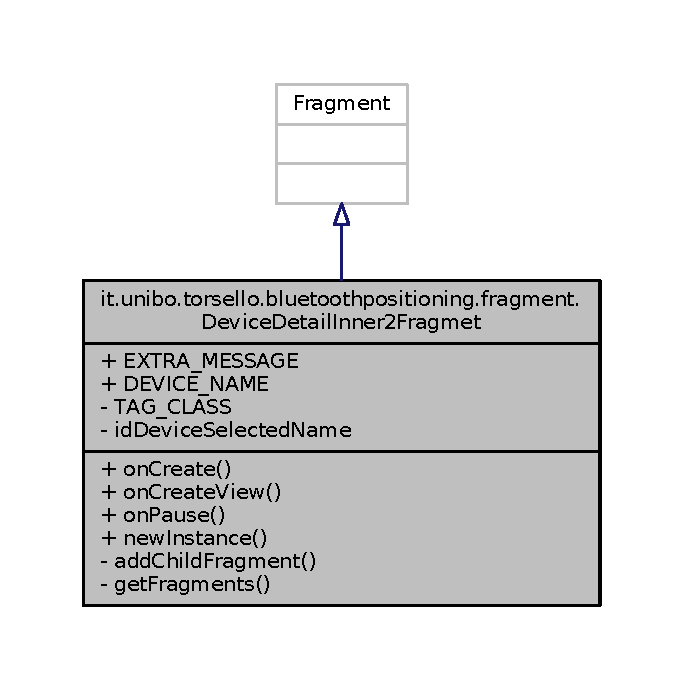
\includegraphics[width=328pt]{classit_1_1unibo_1_1torsello_1_1bluetoothpositioning_1_1fragment_1_1DeviceDetailInner2Fragmet__inherit__graph}
\end{center}
\end{figure}


Diagramma di collaborazione per it.\+unibo.\+torsello.\+bluetoothpositioning.\+fragment.\+Device\+Detail\+Inner2\+Fragmet\+:
\nopagebreak
\begin{figure}[H]
\begin{center}
\leavevmode
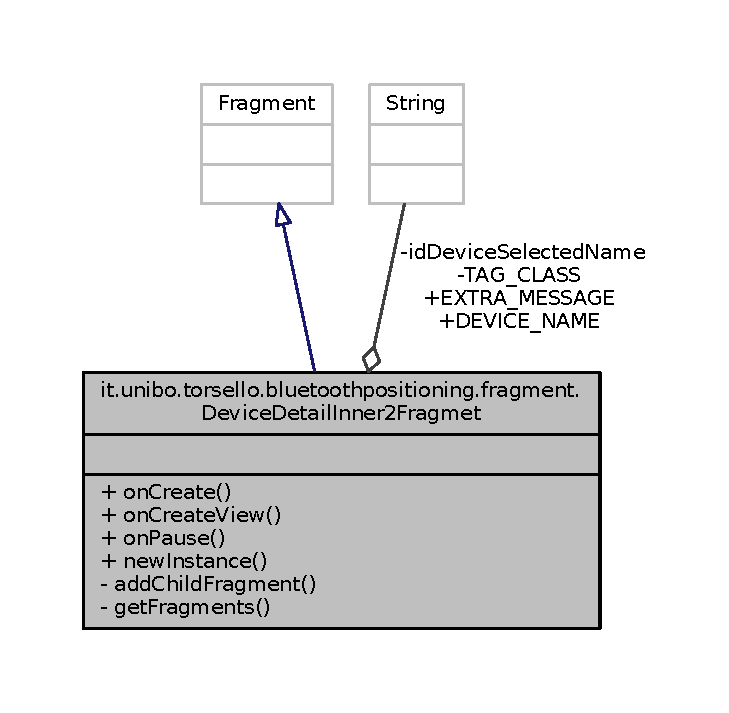
\includegraphics[width=350pt]{classit_1_1unibo_1_1torsello_1_1bluetoothpositioning_1_1fragment_1_1DeviceDetailInner2Fragmet__coll__graph}
\end{center}
\end{figure}
\subsubsection*{Membri pubblici}
\begin{DoxyCompactItemize}
\item 
void \hyperlink{classit_1_1unibo_1_1torsello_1_1bluetoothpositioning_1_1fragment_1_1DeviceDetailInner2Fragmet_ae07630a3636c3acb7b0f353d54a7f816_ae07630a3636c3acb7b0f353d54a7f816}{on\+Create} (Bundle saved\+Instance\+State)
\item 
View \hyperlink{classit_1_1unibo_1_1torsello_1_1bluetoothpositioning_1_1fragment_1_1DeviceDetailInner2Fragmet_a74a36f897121676ecad563c25b484018_a74a36f897121676ecad563c25b484018}{on\+Create\+View} (Layout\+Inflater inflater, View\+Group container, Bundle saved\+Instance\+State)
\item 
void \hyperlink{classit_1_1unibo_1_1torsello_1_1bluetoothpositioning_1_1fragment_1_1DeviceDetailInner2Fragmet_a4adf985f5dee5625553cdde770f82637_a4adf985f5dee5625553cdde770f82637}{on\+Pause} ()
\end{DoxyCompactItemize}
\subsubsection*{Membri pubblici statici}
\begin{DoxyCompactItemize}
\item 
static \hyperlink{classit_1_1unibo_1_1torsello_1_1bluetoothpositioning_1_1fragment_1_1DeviceDetailInner2Fragmet}{Device\+Detail\+Inner2\+Fragmet} \hyperlink{classit_1_1unibo_1_1torsello_1_1bluetoothpositioning_1_1fragment_1_1DeviceDetailInner2Fragmet_a80972a8f816dc07e8844bea60b2438e1_a80972a8f816dc07e8844bea60b2438e1}{new\+Instance} (String message, String device\+Name)
\end{DoxyCompactItemize}
\subsubsection*{Attributi pubblici statici}
\begin{DoxyCompactItemize}
\item 
static final String \hyperlink{classit_1_1unibo_1_1torsello_1_1bluetoothpositioning_1_1fragment_1_1DeviceDetailInner2Fragmet_a2980d3d81aa246caa72f182a8c2ccb11_a2980d3d81aa246caa72f182a8c2ccb11}{E\+X\+T\+R\+A\+\_\+\+M\+E\+S\+S\+A\+GE} = \char`\"{}E\+X\+T\+R\+A\+\_\+\+M\+E\+S\+S\+A\+GE\char`\"{}
\item 
static final String \hyperlink{classit_1_1unibo_1_1torsello_1_1bluetoothpositioning_1_1fragment_1_1DeviceDetailInner2Fragmet_a8e8968fb34c3ad56d582196879b0ef6c_a8e8968fb34c3ad56d582196879b0ef6c}{D\+E\+V\+I\+C\+E\+\_\+\+N\+A\+ME} = \char`\"{}D\+E\+V\+I\+C\+E\+\_\+\+N\+A\+ME\char`\"{}
\end{DoxyCompactItemize}
\subsubsection*{Membri privati}
\begin{DoxyCompactItemize}
\item 
void \hyperlink{classit_1_1unibo_1_1torsello_1_1bluetoothpositioning_1_1fragment_1_1DeviceDetailInner2Fragmet_aa1467621600238fa5efde4a2cee901e0_aa1467621600238fa5efde4a2cee901e0}{add\+Child\+Fragment} (View root)
\item 
Array\+List$<$ Fragment $>$ \hyperlink{classit_1_1unibo_1_1torsello_1_1bluetoothpositioning_1_1fragment_1_1DeviceDetailInner2Fragmet_adc5cddae8abe48105c75060b99937b62_adc5cddae8abe48105c75060b99937b62}{get\+Fragments} ()
\end{DoxyCompactItemize}
\subsubsection*{Attributi privati}
\begin{DoxyCompactItemize}
\item 
final String \hyperlink{classit_1_1unibo_1_1torsello_1_1bluetoothpositioning_1_1fragment_1_1DeviceDetailInner2Fragmet_acd1f1a0a435e383240ad0222c4eb7972_acd1f1a0a435e383240ad0222c4eb7972}{T\+A\+G\+\_\+\+C\+L\+A\+SS} = get\+Class().get\+Simple\+Name()
\item 
String \hyperlink{classit_1_1unibo_1_1torsello_1_1bluetoothpositioning_1_1fragment_1_1DeviceDetailInner2Fragmet_a45380c45eac10e58571b19e50c9fc27c_a45380c45eac10e58571b19e50c9fc27c}{id\+Device\+Selected\+Name}
\end{DoxyCompactItemize}


\subsubsection{Descrizione dettagliata}
Created by federico on 03/10/16. 

\subsubsection{Documentazione delle funzioni membro}
\hypertarget{classit_1_1unibo_1_1torsello_1_1bluetoothpositioning_1_1fragment_1_1DeviceDetailInner2Fragmet_aa1467621600238fa5efde4a2cee901e0_aa1467621600238fa5efde4a2cee901e0}{}\label{classit_1_1unibo_1_1torsello_1_1bluetoothpositioning_1_1fragment_1_1DeviceDetailInner2Fragmet_aa1467621600238fa5efde4a2cee901e0_aa1467621600238fa5efde4a2cee901e0} 
\index{it\+::unibo\+::torsello\+::bluetoothpositioning\+::fragment\+::\+Device\+Detail\+Inner2\+Fragmet@{it\+::unibo\+::torsello\+::bluetoothpositioning\+::fragment\+::\+Device\+Detail\+Inner2\+Fragmet}!add\+Child\+Fragment@{add\+Child\+Fragment}}
\index{add\+Child\+Fragment@{add\+Child\+Fragment}!it\+::unibo\+::torsello\+::bluetoothpositioning\+::fragment\+::\+Device\+Detail\+Inner2\+Fragmet@{it\+::unibo\+::torsello\+::bluetoothpositioning\+::fragment\+::\+Device\+Detail\+Inner2\+Fragmet}}
\paragraph{\texorpdfstring{add\+Child\+Fragment()}{addChildFragment()}}
{\footnotesize\ttfamily void it.\+unibo.\+torsello.\+bluetoothpositioning.\+fragment.\+Device\+Detail\+Inner2\+Fragmet.\+add\+Child\+Fragment (\begin{DoxyParamCaption}\item[{View}]{root }\end{DoxyParamCaption})\hspace{0.3cm}{\ttfamily [private]}}


\begin{DoxyCode}
59                                              \{
60 
61         ViewPager mViewPager = (ViewPager) root.findViewById(R.id.view\_pager);
62         StatePagerAdapter myPageAdapter = \textcolor{keyword}{new} StatePagerAdapter(getChildFragmentManager(), 
      \hyperlink{classit_1_1unibo_1_1torsello_1_1bluetoothpositioning_1_1fragment_1_1DeviceDetailInner2Fragmet_adc5cddae8abe48105c75060b99937b62_adc5cddae8abe48105c75060b99937b62}{getFragments}());
63         mViewPager.setAdapter(myPageAdapter);
64 
65         TabLayout tabLayout = (TabLayout) root.findViewById(R.id.sliding\_tabs);
66         tabLayout.setupWithViewPager(mViewPager);
67     \}
\end{DoxyCode}
\hypertarget{classit_1_1unibo_1_1torsello_1_1bluetoothpositioning_1_1fragment_1_1DeviceDetailInner2Fragmet_adc5cddae8abe48105c75060b99937b62_adc5cddae8abe48105c75060b99937b62}{}\label{classit_1_1unibo_1_1torsello_1_1bluetoothpositioning_1_1fragment_1_1DeviceDetailInner2Fragmet_adc5cddae8abe48105c75060b99937b62_adc5cddae8abe48105c75060b99937b62} 
\index{it\+::unibo\+::torsello\+::bluetoothpositioning\+::fragment\+::\+Device\+Detail\+Inner2\+Fragmet@{it\+::unibo\+::torsello\+::bluetoothpositioning\+::fragment\+::\+Device\+Detail\+Inner2\+Fragmet}!get\+Fragments@{get\+Fragments}}
\index{get\+Fragments@{get\+Fragments}!it\+::unibo\+::torsello\+::bluetoothpositioning\+::fragment\+::\+Device\+Detail\+Inner2\+Fragmet@{it\+::unibo\+::torsello\+::bluetoothpositioning\+::fragment\+::\+Device\+Detail\+Inner2\+Fragmet}}
\paragraph{\texorpdfstring{get\+Fragments()}{getFragments()}}
{\footnotesize\ttfamily Array\+List$<$Fragment$>$ it.\+unibo.\+torsello.\+bluetoothpositioning.\+fragment.\+Device\+Detail\+Inner2\+Fragmet.\+get\+Fragments (\begin{DoxyParamCaption}{ }\end{DoxyParamCaption})\hspace{0.3cm}{\ttfamily [private]}}


\begin{DoxyCode}
69                                                \{
70         ArrayList<Fragment> fragments = \textcolor{keyword}{new} ArrayList<>();
71 
72         \textcolor{comment}{// inner fragment 0}
73         ArrayList<String> params1 = \textcolor{keyword}{new} ArrayList<>();
74         params1.add(getString(R.string.chart\_arduino));
75         params1.add(getString(R.string.chart\_raw\_distance));
76         params1.add(getString(R.string.chart\_altbeacon));
77         params1.add(getString(R.string.chart\_kalman\_filter));
78 
79         fragments.add(DeviceChartFragment.newInstance(\textcolor{stringliteral}{"chart1"}, 
      \hyperlink{classit_1_1unibo_1_1torsello_1_1bluetoothpositioning_1_1fragment_1_1DeviceDetailInner2Fragmet_a45380c45eac10e58571b19e50c9fc27c_a45380c45eac10e58571b19e50c9fc27c}{idDeviceSelectedName}, params1));
80 
81         \textcolor{comment}{// inner fragment 1}
82         ArrayList<String> params2 = \textcolor{keyword}{new} ArrayList<>();
83         params2.add(getString(R.string.chart\_arduino));
84         params2.add(getString(R.string.chart\_raw\_distance));
85         params2.add(getString(R.string.chart\_kalman\_filter));
86 
87         fragments.add(DeviceChartFragment.newInstance(\textcolor{stringliteral}{"chart2"}, 
      \hyperlink{classit_1_1unibo_1_1torsello_1_1bluetoothpositioning_1_1fragment_1_1DeviceDetailInner2Fragmet_a45380c45eac10e58571b19e50c9fc27c_a45380c45eac10e58571b19e50c9fc27c}{idDeviceSelectedName}, params2));
88 
89         \textcolor{comment}{// inner fragment 2}
90         ArrayList<String> params3 = \textcolor{keyword}{new} ArrayList<>();
91         params3.add(getString(R.string.chart\_arduino));
92         params3.add(getString(R.string.chart\_altbeacon));
93         params3.add(getString(R.string.chart\_kalman\_filter));
94 
95         fragments.add(DeviceChartFragment.newInstance(\textcolor{stringliteral}{"chart3"}, 
      \hyperlink{classit_1_1unibo_1_1torsello_1_1bluetoothpositioning_1_1fragment_1_1DeviceDetailInner2Fragmet_a45380c45eac10e58571b19e50c9fc27c_a45380c45eac10e58571b19e50c9fc27c}{idDeviceSelectedName}, params3));
96 
97         \textcolor{keywordflow}{return} fragments;
98     \}
\end{DoxyCode}
\hypertarget{classit_1_1unibo_1_1torsello_1_1bluetoothpositioning_1_1fragment_1_1DeviceDetailInner2Fragmet_a80972a8f816dc07e8844bea60b2438e1_a80972a8f816dc07e8844bea60b2438e1}{}\label{classit_1_1unibo_1_1torsello_1_1bluetoothpositioning_1_1fragment_1_1DeviceDetailInner2Fragmet_a80972a8f816dc07e8844bea60b2438e1_a80972a8f816dc07e8844bea60b2438e1} 
\index{it\+::unibo\+::torsello\+::bluetoothpositioning\+::fragment\+::\+Device\+Detail\+Inner2\+Fragmet@{it\+::unibo\+::torsello\+::bluetoothpositioning\+::fragment\+::\+Device\+Detail\+Inner2\+Fragmet}!new\+Instance@{new\+Instance}}
\index{new\+Instance@{new\+Instance}!it\+::unibo\+::torsello\+::bluetoothpositioning\+::fragment\+::\+Device\+Detail\+Inner2\+Fragmet@{it\+::unibo\+::torsello\+::bluetoothpositioning\+::fragment\+::\+Device\+Detail\+Inner2\+Fragmet}}
\paragraph{\texorpdfstring{new\+Instance()}{newInstance()}}
{\footnotesize\ttfamily static \hyperlink{classit_1_1unibo_1_1torsello_1_1bluetoothpositioning_1_1fragment_1_1DeviceDetailInner2Fragmet}{Device\+Detail\+Inner2\+Fragmet} it.\+unibo.\+torsello.\+bluetoothpositioning.\+fragment.\+Device\+Detail\+Inner2\+Fragmet.\+new\+Instance (\begin{DoxyParamCaption}\item[{String}]{message,  }\item[{String}]{device\+Name }\end{DoxyParamCaption})\hspace{0.3cm}{\ttfamily [static]}}


\begin{DoxyCode}
29                                                                                            \{
30         DeviceDetailInner2Fragmet fragment = \textcolor{keyword}{new} DeviceDetailInner2Fragmet();
31         Bundle args = \textcolor{keyword}{new} Bundle();
32         args.putString(\hyperlink{classit_1_1unibo_1_1torsello_1_1bluetoothpositioning_1_1fragment_1_1DeviceDetailInner2Fragmet_a2980d3d81aa246caa72f182a8c2ccb11_a2980d3d81aa246caa72f182a8c2ccb11}{EXTRA\_MESSAGE}, message);
33         args.putString(\hyperlink{classit_1_1unibo_1_1torsello_1_1bluetoothpositioning_1_1fragment_1_1DeviceDetailInner2Fragmet_a8e8968fb34c3ad56d582196879b0ef6c_a8e8968fb34c3ad56d582196879b0ef6c}{DEVICE\_NAME}, deviceName);
34         fragment.setArguments(args);
35         \textcolor{keywordflow}{return} fragment;
36     \}
\end{DoxyCode}
\hypertarget{classit_1_1unibo_1_1torsello_1_1bluetoothpositioning_1_1fragment_1_1DeviceDetailInner2Fragmet_ae07630a3636c3acb7b0f353d54a7f816_ae07630a3636c3acb7b0f353d54a7f816}{}\label{classit_1_1unibo_1_1torsello_1_1bluetoothpositioning_1_1fragment_1_1DeviceDetailInner2Fragmet_ae07630a3636c3acb7b0f353d54a7f816_ae07630a3636c3acb7b0f353d54a7f816} 
\index{it\+::unibo\+::torsello\+::bluetoothpositioning\+::fragment\+::\+Device\+Detail\+Inner2\+Fragmet@{it\+::unibo\+::torsello\+::bluetoothpositioning\+::fragment\+::\+Device\+Detail\+Inner2\+Fragmet}!on\+Create@{on\+Create}}
\index{on\+Create@{on\+Create}!it\+::unibo\+::torsello\+::bluetoothpositioning\+::fragment\+::\+Device\+Detail\+Inner2\+Fragmet@{it\+::unibo\+::torsello\+::bluetoothpositioning\+::fragment\+::\+Device\+Detail\+Inner2\+Fragmet}}
\paragraph{\texorpdfstring{on\+Create()}{onCreate()}}
{\footnotesize\ttfamily void it.\+unibo.\+torsello.\+bluetoothpositioning.\+fragment.\+Device\+Detail\+Inner2\+Fragmet.\+on\+Create (\begin{DoxyParamCaption}\item[{Bundle}]{saved\+Instance\+State }\end{DoxyParamCaption})}


\begin{DoxyCode}
39                                                     \{
40         super.onCreate(savedInstanceState);
41 
42         \hyperlink{classit_1_1unibo_1_1torsello_1_1bluetoothpositioning_1_1fragment_1_1DeviceDetailInner2Fragmet_a45380c45eac10e58571b19e50c9fc27c_a45380c45eac10e58571b19e50c9fc27c}{idDeviceSelectedName} = getArguments().getString(
      \hyperlink{classit_1_1unibo_1_1torsello_1_1bluetoothpositioning_1_1fragment_1_1DeviceDetailInner2Fragmet_a8e8968fb34c3ad56d582196879b0ef6c_a8e8968fb34c3ad56d582196879b0ef6c}{DEVICE\_NAME});
43     \}
\end{DoxyCode}
\hypertarget{classit_1_1unibo_1_1torsello_1_1bluetoothpositioning_1_1fragment_1_1DeviceDetailInner2Fragmet_a74a36f897121676ecad563c25b484018_a74a36f897121676ecad563c25b484018}{}\label{classit_1_1unibo_1_1torsello_1_1bluetoothpositioning_1_1fragment_1_1DeviceDetailInner2Fragmet_a74a36f897121676ecad563c25b484018_a74a36f897121676ecad563c25b484018} 
\index{it\+::unibo\+::torsello\+::bluetoothpositioning\+::fragment\+::\+Device\+Detail\+Inner2\+Fragmet@{it\+::unibo\+::torsello\+::bluetoothpositioning\+::fragment\+::\+Device\+Detail\+Inner2\+Fragmet}!on\+Create\+View@{on\+Create\+View}}
\index{on\+Create\+View@{on\+Create\+View}!it\+::unibo\+::torsello\+::bluetoothpositioning\+::fragment\+::\+Device\+Detail\+Inner2\+Fragmet@{it\+::unibo\+::torsello\+::bluetoothpositioning\+::fragment\+::\+Device\+Detail\+Inner2\+Fragmet}}
\paragraph{\texorpdfstring{on\+Create\+View()}{onCreateView()}}
{\footnotesize\ttfamily View it.\+unibo.\+torsello.\+bluetoothpositioning.\+fragment.\+Device\+Detail\+Inner2\+Fragmet.\+on\+Create\+View (\begin{DoxyParamCaption}\item[{Layout\+Inflater}]{inflater,  }\item[{View\+Group}]{container,  }\item[{Bundle}]{saved\+Instance\+State }\end{DoxyParamCaption})}


\begin{DoxyCode}
46                                                                                                       \{
47         View root = inflater.inflate(R.layout.fragment\_device\_detail\_inner\_2, container, \textcolor{keyword}{false});
48 
49         \hyperlink{classit_1_1unibo_1_1torsello_1_1bluetoothpositioning_1_1fragment_1_1DeviceDetailInner2Fragmet_aa1467621600238fa5efde4a2cee901e0_aa1467621600238fa5efde4a2cee901e0}{addChildFragment}(root);
50 
51         \textcolor{keywordflow}{return} root;
52     \}
\end{DoxyCode}
\hypertarget{classit_1_1unibo_1_1torsello_1_1bluetoothpositioning_1_1fragment_1_1DeviceDetailInner2Fragmet_a4adf985f5dee5625553cdde770f82637_a4adf985f5dee5625553cdde770f82637}{}\label{classit_1_1unibo_1_1torsello_1_1bluetoothpositioning_1_1fragment_1_1DeviceDetailInner2Fragmet_a4adf985f5dee5625553cdde770f82637_a4adf985f5dee5625553cdde770f82637} 
\index{it\+::unibo\+::torsello\+::bluetoothpositioning\+::fragment\+::\+Device\+Detail\+Inner2\+Fragmet@{it\+::unibo\+::torsello\+::bluetoothpositioning\+::fragment\+::\+Device\+Detail\+Inner2\+Fragmet}!on\+Pause@{on\+Pause}}
\index{on\+Pause@{on\+Pause}!it\+::unibo\+::torsello\+::bluetoothpositioning\+::fragment\+::\+Device\+Detail\+Inner2\+Fragmet@{it\+::unibo\+::torsello\+::bluetoothpositioning\+::fragment\+::\+Device\+Detail\+Inner2\+Fragmet}}
\paragraph{\texorpdfstring{on\+Pause()}{onPause()}}
{\footnotesize\ttfamily void it.\+unibo.\+torsello.\+bluetoothpositioning.\+fragment.\+Device\+Detail\+Inner2\+Fragmet.\+on\+Pause (\begin{DoxyParamCaption}{ }\end{DoxyParamCaption})}


\begin{DoxyCode}
55                           \{
56         super.onPause();
57     \}
\end{DoxyCode}


\subsubsection{Documentazione dei membri dato}
\hypertarget{classit_1_1unibo_1_1torsello_1_1bluetoothpositioning_1_1fragment_1_1DeviceDetailInner2Fragmet_a8e8968fb34c3ad56d582196879b0ef6c_a8e8968fb34c3ad56d582196879b0ef6c}{}\label{classit_1_1unibo_1_1torsello_1_1bluetoothpositioning_1_1fragment_1_1DeviceDetailInner2Fragmet_a8e8968fb34c3ad56d582196879b0ef6c_a8e8968fb34c3ad56d582196879b0ef6c} 
\index{it\+::unibo\+::torsello\+::bluetoothpositioning\+::fragment\+::\+Device\+Detail\+Inner2\+Fragmet@{it\+::unibo\+::torsello\+::bluetoothpositioning\+::fragment\+::\+Device\+Detail\+Inner2\+Fragmet}!D\+E\+V\+I\+C\+E\+\_\+\+N\+A\+ME@{D\+E\+V\+I\+C\+E\+\_\+\+N\+A\+ME}}
\index{D\+E\+V\+I\+C\+E\+\_\+\+N\+A\+ME@{D\+E\+V\+I\+C\+E\+\_\+\+N\+A\+ME}!it\+::unibo\+::torsello\+::bluetoothpositioning\+::fragment\+::\+Device\+Detail\+Inner2\+Fragmet@{it\+::unibo\+::torsello\+::bluetoothpositioning\+::fragment\+::\+Device\+Detail\+Inner2\+Fragmet}}
\paragraph{\texorpdfstring{D\+E\+V\+I\+C\+E\+\_\+\+N\+A\+ME}{DEVICE\_NAME}}
{\footnotesize\ttfamily final String it.\+unibo.\+torsello.\+bluetoothpositioning.\+fragment.\+Device\+Detail\+Inner2\+Fragmet.\+D\+E\+V\+I\+C\+E\+\_\+\+N\+A\+ME = \char`\"{}D\+E\+V\+I\+C\+E\+\_\+\+N\+A\+ME\char`\"{}\hspace{0.3cm}{\ttfamily [static]}}

\hypertarget{classit_1_1unibo_1_1torsello_1_1bluetoothpositioning_1_1fragment_1_1DeviceDetailInner2Fragmet_a2980d3d81aa246caa72f182a8c2ccb11_a2980d3d81aa246caa72f182a8c2ccb11}{}\label{classit_1_1unibo_1_1torsello_1_1bluetoothpositioning_1_1fragment_1_1DeviceDetailInner2Fragmet_a2980d3d81aa246caa72f182a8c2ccb11_a2980d3d81aa246caa72f182a8c2ccb11} 
\index{it\+::unibo\+::torsello\+::bluetoothpositioning\+::fragment\+::\+Device\+Detail\+Inner2\+Fragmet@{it\+::unibo\+::torsello\+::bluetoothpositioning\+::fragment\+::\+Device\+Detail\+Inner2\+Fragmet}!E\+X\+T\+R\+A\+\_\+\+M\+E\+S\+S\+A\+GE@{E\+X\+T\+R\+A\+\_\+\+M\+E\+S\+S\+A\+GE}}
\index{E\+X\+T\+R\+A\+\_\+\+M\+E\+S\+S\+A\+GE@{E\+X\+T\+R\+A\+\_\+\+M\+E\+S\+S\+A\+GE}!it\+::unibo\+::torsello\+::bluetoothpositioning\+::fragment\+::\+Device\+Detail\+Inner2\+Fragmet@{it\+::unibo\+::torsello\+::bluetoothpositioning\+::fragment\+::\+Device\+Detail\+Inner2\+Fragmet}}
\paragraph{\texorpdfstring{E\+X\+T\+R\+A\+\_\+\+M\+E\+S\+S\+A\+GE}{EXTRA\_MESSAGE}}
{\footnotesize\ttfamily final String it.\+unibo.\+torsello.\+bluetoothpositioning.\+fragment.\+Device\+Detail\+Inner2\+Fragmet.\+E\+X\+T\+R\+A\+\_\+\+M\+E\+S\+S\+A\+GE = \char`\"{}E\+X\+T\+R\+A\+\_\+\+M\+E\+S\+S\+A\+GE\char`\"{}\hspace{0.3cm}{\ttfamily [static]}}

\hypertarget{classit_1_1unibo_1_1torsello_1_1bluetoothpositioning_1_1fragment_1_1DeviceDetailInner2Fragmet_a45380c45eac10e58571b19e50c9fc27c_a45380c45eac10e58571b19e50c9fc27c}{}\label{classit_1_1unibo_1_1torsello_1_1bluetoothpositioning_1_1fragment_1_1DeviceDetailInner2Fragmet_a45380c45eac10e58571b19e50c9fc27c_a45380c45eac10e58571b19e50c9fc27c} 
\index{it\+::unibo\+::torsello\+::bluetoothpositioning\+::fragment\+::\+Device\+Detail\+Inner2\+Fragmet@{it\+::unibo\+::torsello\+::bluetoothpositioning\+::fragment\+::\+Device\+Detail\+Inner2\+Fragmet}!id\+Device\+Selected\+Name@{id\+Device\+Selected\+Name}}
\index{id\+Device\+Selected\+Name@{id\+Device\+Selected\+Name}!it\+::unibo\+::torsello\+::bluetoothpositioning\+::fragment\+::\+Device\+Detail\+Inner2\+Fragmet@{it\+::unibo\+::torsello\+::bluetoothpositioning\+::fragment\+::\+Device\+Detail\+Inner2\+Fragmet}}
\paragraph{\texorpdfstring{id\+Device\+Selected\+Name}{idDeviceSelectedName}}
{\footnotesize\ttfamily String it.\+unibo.\+torsello.\+bluetoothpositioning.\+fragment.\+Device\+Detail\+Inner2\+Fragmet.\+id\+Device\+Selected\+Name\hspace{0.3cm}{\ttfamily [private]}}

\hypertarget{classit_1_1unibo_1_1torsello_1_1bluetoothpositioning_1_1fragment_1_1DeviceDetailInner2Fragmet_acd1f1a0a435e383240ad0222c4eb7972_acd1f1a0a435e383240ad0222c4eb7972}{}\label{classit_1_1unibo_1_1torsello_1_1bluetoothpositioning_1_1fragment_1_1DeviceDetailInner2Fragmet_acd1f1a0a435e383240ad0222c4eb7972_acd1f1a0a435e383240ad0222c4eb7972} 
\index{it\+::unibo\+::torsello\+::bluetoothpositioning\+::fragment\+::\+Device\+Detail\+Inner2\+Fragmet@{it\+::unibo\+::torsello\+::bluetoothpositioning\+::fragment\+::\+Device\+Detail\+Inner2\+Fragmet}!T\+A\+G\+\_\+\+C\+L\+A\+SS@{T\+A\+G\+\_\+\+C\+L\+A\+SS}}
\index{T\+A\+G\+\_\+\+C\+L\+A\+SS@{T\+A\+G\+\_\+\+C\+L\+A\+SS}!it\+::unibo\+::torsello\+::bluetoothpositioning\+::fragment\+::\+Device\+Detail\+Inner2\+Fragmet@{it\+::unibo\+::torsello\+::bluetoothpositioning\+::fragment\+::\+Device\+Detail\+Inner2\+Fragmet}}
\paragraph{\texorpdfstring{T\+A\+G\+\_\+\+C\+L\+A\+SS}{TAG\_CLASS}}
{\footnotesize\ttfamily final String it.\+unibo.\+torsello.\+bluetoothpositioning.\+fragment.\+Device\+Detail\+Inner2\+Fragmet.\+T\+A\+G\+\_\+\+C\+L\+A\+SS = get\+Class().get\+Simple\+Name()\hspace{0.3cm}{\ttfamily [private]}}



La documentazione per questa classe è stata generata a partire dal seguente file\+:\begin{DoxyCompactItemize}
\item 
\hyperlink{DeviceDetailInner2Fragmet_8java}{Device\+Detail\+Inner2\+Fragmet.\+java}\end{DoxyCompactItemize}

\hypertarget{classit_1_1unibo_1_1torsello_1_1bluetoothpositioning_1_1fragment_1_1devicesObservers_1_1DeviceListFragment}{}\subsection{Riferimenti per la classe it.\+unibo.\+torsello.\+bluetoothpositioning.\+fragment.\+devices\+Observers.\+Device\+List\+Fragment}
\label{classit_1_1unibo_1_1torsello_1_1bluetoothpositioning_1_1fragment_1_1devicesObservers_1_1DeviceListFragment}\index{it.\+unibo.\+torsello.\+bluetoothpositioning.\+fragment.\+devices\+Observers.\+Device\+List\+Fragment@{it.\+unibo.\+torsello.\+bluetoothpositioning.\+fragment.\+devices\+Observers.\+Device\+List\+Fragment}}


Diagramma delle classi per it.\+unibo.\+torsello.\+bluetoothpositioning.\+fragment.\+devices\+Observers.\+Device\+List\+Fragment
\nopagebreak
\begin{figure}[H]
\begin{center}
\leavevmode
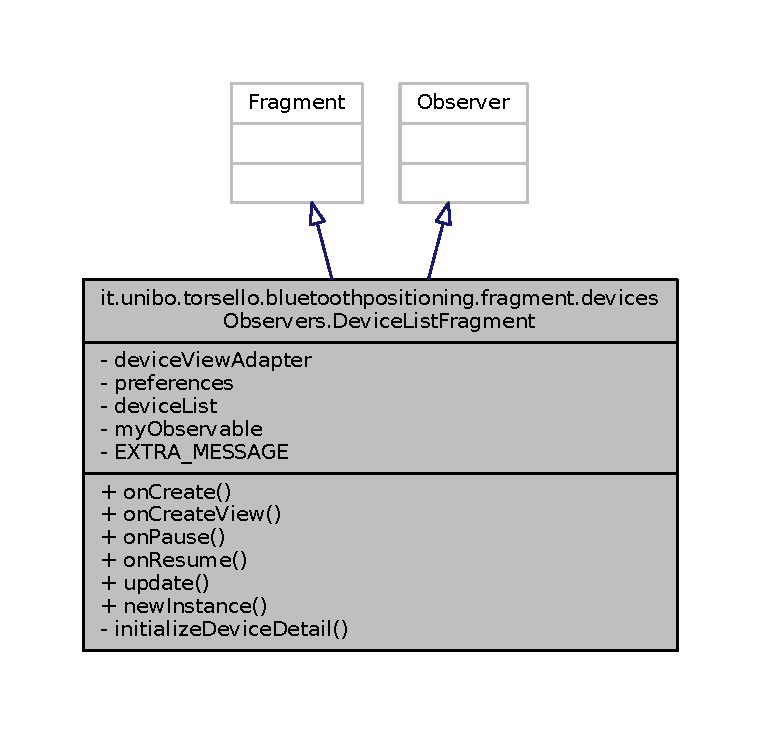
\includegraphics[width=350pt]{classit_1_1unibo_1_1torsello_1_1bluetoothpositioning_1_1fragment_1_1devicesObservers_1_1DeviceListFragment__inherit__graph}
\end{center}
\end{figure}


Diagramma di collaborazione per it.\+unibo.\+torsello.\+bluetoothpositioning.\+fragment.\+devices\+Observers.\+Device\+List\+Fragment\+:
\nopagebreak
\begin{figure}[H]
\begin{center}
\leavevmode
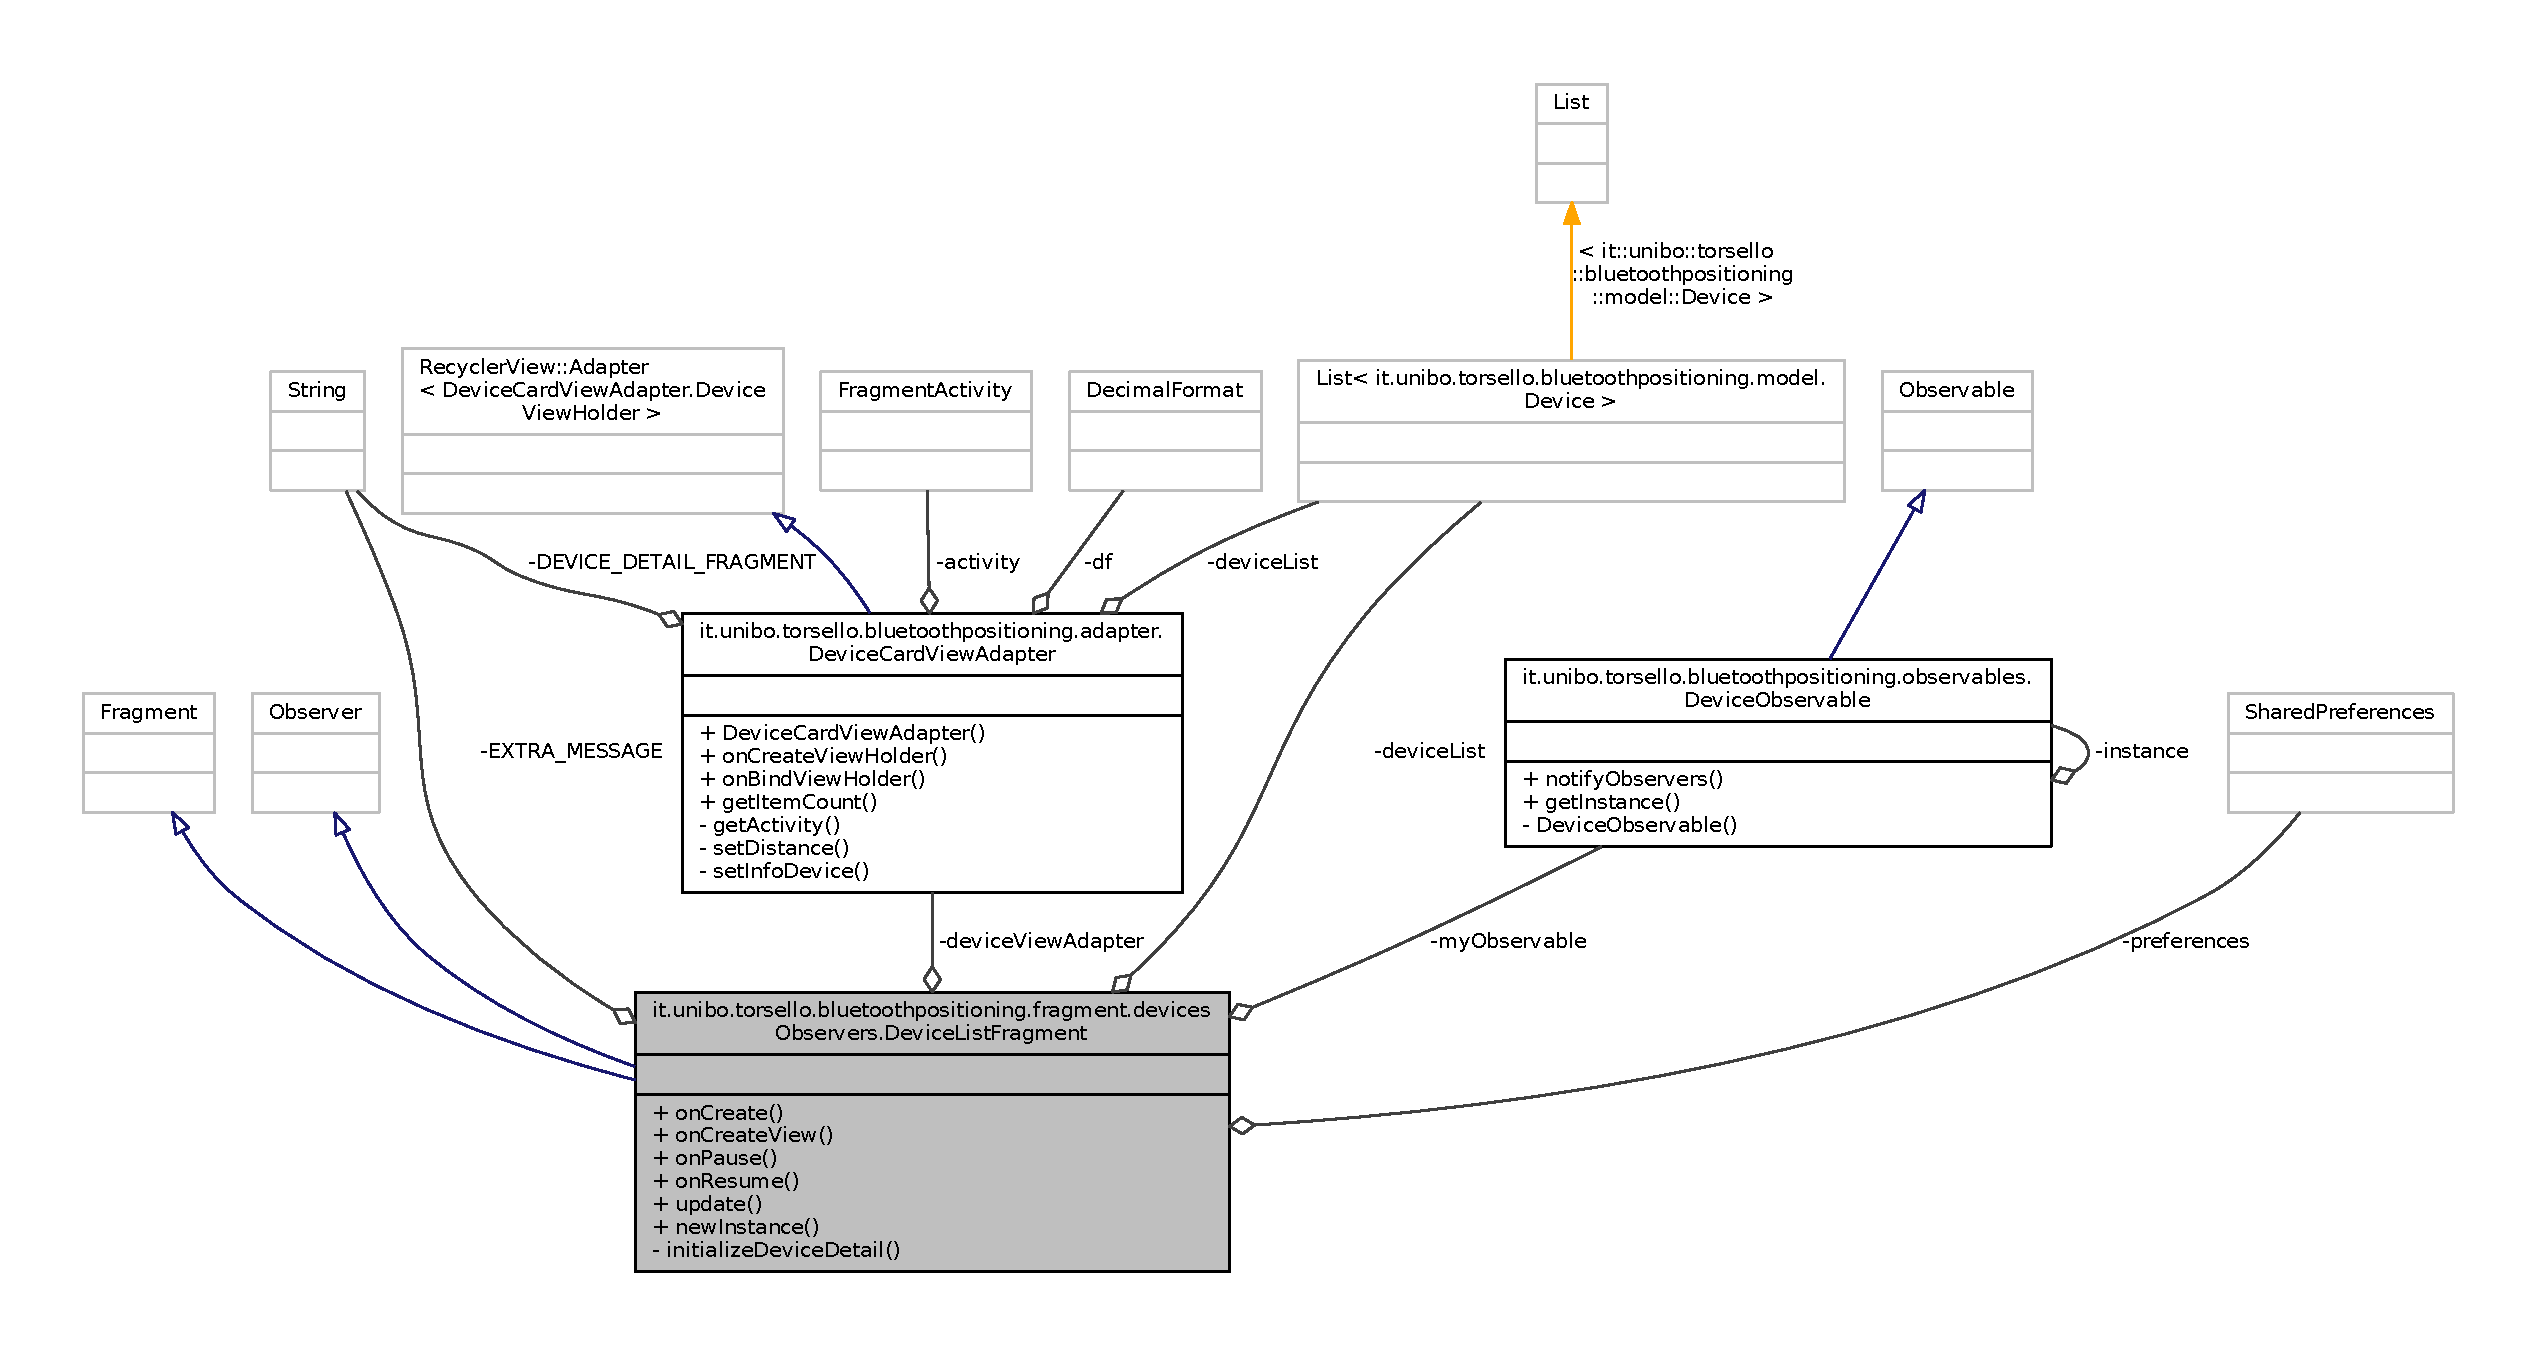
\includegraphics[width=350pt]{classit_1_1unibo_1_1torsello_1_1bluetoothpositioning_1_1fragment_1_1devicesObservers_1_1DeviceListFragment__coll__graph}
\end{center}
\end{figure}
\subsubsection*{Membri pubblici}
\begin{DoxyCompactItemize}
\item 
void \hyperlink{classit_1_1unibo_1_1torsello_1_1bluetoothpositioning_1_1fragment_1_1devicesObservers_1_1DeviceListFragment_a5e548142d1a24ac89205c9e2adac82b6_a5e548142d1a24ac89205c9e2adac82b6}{on\+Create} (@Nullable Bundle saved\+Instance\+State)
\item 
View \hyperlink{classit_1_1unibo_1_1torsello_1_1bluetoothpositioning_1_1fragment_1_1devicesObservers_1_1DeviceListFragment_a7897dd7ea0239d171ec620f65607cc3a_a7897dd7ea0239d171ec620f65607cc3a}{on\+Create\+View} (Layout\+Inflater inflater, View\+Group container, Bundle saved\+Instance\+State)
\item 
void \hyperlink{classit_1_1unibo_1_1torsello_1_1bluetoothpositioning_1_1fragment_1_1devicesObservers_1_1DeviceListFragment_abf68ff973b31bc3d26c1812bffefc2ac_abf68ff973b31bc3d26c1812bffefc2ac}{on\+Pause} ()
\item 
void \hyperlink{classit_1_1unibo_1_1torsello_1_1bluetoothpositioning_1_1fragment_1_1devicesObservers_1_1DeviceListFragment_a8cc0bafb039909424861854606d51b11_a8cc0bafb039909424861854606d51b11}{on\+Resume} ()
\item 
void \hyperlink{classit_1_1unibo_1_1torsello_1_1bluetoothpositioning_1_1fragment_1_1devicesObservers_1_1DeviceListFragment_a9703aa2a0185098c909173d3b49cb448_a9703aa2a0185098c909173d3b49cb448}{update} (Observable o, Object arg)
\end{DoxyCompactItemize}
\subsubsection*{Membri pubblici statici}
\begin{DoxyCompactItemize}
\item 
static \hyperlink{classit_1_1unibo_1_1torsello_1_1bluetoothpositioning_1_1fragment_1_1devicesObservers_1_1DeviceListFragment}{Device\+List\+Fragment} \hyperlink{classit_1_1unibo_1_1torsello_1_1bluetoothpositioning_1_1fragment_1_1devicesObservers_1_1DeviceListFragment_aae7377d92372118bec0bd8a6aa2c61c0_aae7377d92372118bec0bd8a6aa2c61c0}{new\+Instance} ()
\end{DoxyCompactItemize}
\subsubsection*{Membri privati}
\begin{DoxyCompactItemize}
\item 
void \hyperlink{classit_1_1unibo_1_1torsello_1_1bluetoothpositioning_1_1fragment_1_1devicesObservers_1_1DeviceListFragment_a34eb53805cb490013ab68ee251bdf473_a34eb53805cb490013ab68ee251bdf473}{initialize\+Device\+Detail} (View root)
\end{DoxyCompactItemize}
\subsubsection*{Attributi privati}
\begin{DoxyCompactItemize}
\item 
\hyperlink{classit_1_1unibo_1_1torsello_1_1bluetoothpositioning_1_1adapter_1_1DeviceCardViewAdapter}{Device\+Card\+View\+Adapter} \hyperlink{classit_1_1unibo_1_1torsello_1_1bluetoothpositioning_1_1fragment_1_1devicesObservers_1_1DeviceListFragment_a5a6d0882c9d5551b13936776fb712b0a_a5a6d0882c9d5551b13936776fb712b0a}{device\+View\+Adapter}
\item 
Shared\+Preferences \hyperlink{classit_1_1unibo_1_1torsello_1_1bluetoothpositioning_1_1fragment_1_1devicesObservers_1_1DeviceListFragment_ac2b5a8b56dc71b8a217dbc37515e2052_ac2b5a8b56dc71b8a217dbc37515e2052}{preferences}
\item 
List$<$ \hyperlink{classit_1_1unibo_1_1torsello_1_1bluetoothpositioning_1_1model_1_1Device}{Device} $>$ \hyperlink{classit_1_1unibo_1_1torsello_1_1bluetoothpositioning_1_1fragment_1_1devicesObservers_1_1DeviceListFragment_ad728f2e256af2d4acf05d3cf900f3ad4_ad728f2e256af2d4acf05d3cf900f3ad4}{device\+List}
\item 
\hyperlink{classit_1_1unibo_1_1torsello_1_1bluetoothpositioning_1_1observables_1_1DeviceObservable}{Device\+Observable} \hyperlink{classit_1_1unibo_1_1torsello_1_1bluetoothpositioning_1_1fragment_1_1devicesObservers_1_1DeviceListFragment_a437b28a367ed0f3f5f26e7994b10675d_a437b28a367ed0f3f5f26e7994b10675d}{my\+Observable}
\end{DoxyCompactItemize}
\subsubsection*{Attributi privati statici}
\begin{DoxyCompactItemize}
\item 
static final String \hyperlink{classit_1_1unibo_1_1torsello_1_1bluetoothpositioning_1_1fragment_1_1devicesObservers_1_1DeviceListFragment_a6ba928c98442b32c8a32eb35b7cecf45_a6ba928c98442b32c8a32eb35b7cecf45}{E\+X\+T\+R\+A\+\_\+\+M\+E\+S\+S\+A\+GE} = \char`\"{}E\+X\+T\+R\+A\+\_\+\+M\+E\+S\+S\+A\+GE\char`\"{}
\end{DoxyCompactItemize}


\subsubsection{Descrizione dettagliata}
Created by Federico Torsello. \href{mailto:federico.torsello@studio.unibo.it}{\tt federico.\+torsello@studio.\+unibo.\+it} 

\subsubsection{Documentazione delle funzioni membro}
\hypertarget{classit_1_1unibo_1_1torsello_1_1bluetoothpositioning_1_1fragment_1_1devicesObservers_1_1DeviceListFragment_a34eb53805cb490013ab68ee251bdf473_a34eb53805cb490013ab68ee251bdf473}{}\label{classit_1_1unibo_1_1torsello_1_1bluetoothpositioning_1_1fragment_1_1devicesObservers_1_1DeviceListFragment_a34eb53805cb490013ab68ee251bdf473_a34eb53805cb490013ab68ee251bdf473} 
\index{it\+::unibo\+::torsello\+::bluetoothpositioning\+::fragment\+::devices\+Observers\+::\+Device\+List\+Fragment@{it\+::unibo\+::torsello\+::bluetoothpositioning\+::fragment\+::devices\+Observers\+::\+Device\+List\+Fragment}!initialize\+Device\+Detail@{initialize\+Device\+Detail}}
\index{initialize\+Device\+Detail@{initialize\+Device\+Detail}!it\+::unibo\+::torsello\+::bluetoothpositioning\+::fragment\+::devices\+Observers\+::\+Device\+List\+Fragment@{it\+::unibo\+::torsello\+::bluetoothpositioning\+::fragment\+::devices\+Observers\+::\+Device\+List\+Fragment}}
\paragraph{\texorpdfstring{initialize\+Device\+Detail()}{initializeDeviceDetail()}}
{\footnotesize\ttfamily void it.\+unibo.\+torsello.\+bluetoothpositioning.\+fragment.\+devices\+Observers.\+Device\+List\+Fragment.\+initialize\+Device\+Detail (\begin{DoxyParamCaption}\item[{View}]{root }\end{DoxyParamCaption})\hspace{0.3cm}{\ttfamily [private]}}


\begin{DoxyCode}
84                                                    \{
85         \textcolor{comment}{// add RecyclerView}
86         RecyclerView recyclerView = (RecyclerView) root.findViewById(R.id.recycler\_view);
87         recyclerView.setLayoutManager(\textcolor{keyword}{new} LinearLayoutManager(getContext()));
88         \hyperlink{classit_1_1unibo_1_1torsello_1_1bluetoothpositioning_1_1fragment_1_1devicesObservers_1_1DeviceListFragment_a5a6d0882c9d5551b13936776fb712b0a_a5a6d0882c9d5551b13936776fb712b0a}{deviceViewAdapter} = \textcolor{keyword}{new} DeviceCardViewAdapter(getActivity(), 
      \hyperlink{classit_1_1unibo_1_1torsello_1_1bluetoothpositioning_1_1fragment_1_1devicesObservers_1_1DeviceListFragment_ad728f2e256af2d4acf05d3cf900f3ad4_ad728f2e256af2d4acf05d3cf900f3ad4}{deviceList});
89         recyclerView.setAdapter(\hyperlink{classit_1_1unibo_1_1torsello_1_1bluetoothpositioning_1_1fragment_1_1devicesObservers_1_1DeviceListFragment_a5a6d0882c9d5551b13936776fb712b0a_a5a6d0882c9d5551b13936776fb712b0a}{deviceViewAdapter});
90     \}
\end{DoxyCode}
\hypertarget{classit_1_1unibo_1_1torsello_1_1bluetoothpositioning_1_1fragment_1_1devicesObservers_1_1DeviceListFragment_aae7377d92372118bec0bd8a6aa2c61c0_aae7377d92372118bec0bd8a6aa2c61c0}{}\label{classit_1_1unibo_1_1torsello_1_1bluetoothpositioning_1_1fragment_1_1devicesObservers_1_1DeviceListFragment_aae7377d92372118bec0bd8a6aa2c61c0_aae7377d92372118bec0bd8a6aa2c61c0} 
\index{it\+::unibo\+::torsello\+::bluetoothpositioning\+::fragment\+::devices\+Observers\+::\+Device\+List\+Fragment@{it\+::unibo\+::torsello\+::bluetoothpositioning\+::fragment\+::devices\+Observers\+::\+Device\+List\+Fragment}!new\+Instance@{new\+Instance}}
\index{new\+Instance@{new\+Instance}!it\+::unibo\+::torsello\+::bluetoothpositioning\+::fragment\+::devices\+Observers\+::\+Device\+List\+Fragment@{it\+::unibo\+::torsello\+::bluetoothpositioning\+::fragment\+::devices\+Observers\+::\+Device\+List\+Fragment}}
\paragraph{\texorpdfstring{new\+Instance()}{newInstance()}}
{\footnotesize\ttfamily static \hyperlink{classit_1_1unibo_1_1torsello_1_1bluetoothpositioning_1_1fragment_1_1devicesObservers_1_1DeviceListFragment}{Device\+List\+Fragment} it.\+unibo.\+torsello.\+bluetoothpositioning.\+fragment.\+devices\+Observers.\+Device\+List\+Fragment.\+new\+Instance (\begin{DoxyParamCaption}{ }\end{DoxyParamCaption})\hspace{0.3cm}{\ttfamily [static]}}


\begin{DoxyCode}
56                                                    \{
57         DeviceListFragment fragment = \textcolor{keyword}{new} DeviceListFragment();
58         Bundle args = \textcolor{keyword}{new} Bundle();
59         args.putString(\hyperlink{classit_1_1unibo_1_1torsello_1_1bluetoothpositioning_1_1fragment_1_1devicesObservers_1_1DeviceListFragment_a6ba928c98442b32c8a32eb35b7cecf45_a6ba928c98442b32c8a32eb35b7cecf45}{EXTRA\_MESSAGE}, \textcolor{stringliteral}{"Scan Device"});
60         fragment.setArguments(args);
61         \textcolor{keywordflow}{return} fragment;
62     \}
\end{DoxyCode}
\hypertarget{classit_1_1unibo_1_1torsello_1_1bluetoothpositioning_1_1fragment_1_1devicesObservers_1_1DeviceListFragment_a5e548142d1a24ac89205c9e2adac82b6_a5e548142d1a24ac89205c9e2adac82b6}{}\label{classit_1_1unibo_1_1torsello_1_1bluetoothpositioning_1_1fragment_1_1devicesObservers_1_1DeviceListFragment_a5e548142d1a24ac89205c9e2adac82b6_a5e548142d1a24ac89205c9e2adac82b6} 
\index{it\+::unibo\+::torsello\+::bluetoothpositioning\+::fragment\+::devices\+Observers\+::\+Device\+List\+Fragment@{it\+::unibo\+::torsello\+::bluetoothpositioning\+::fragment\+::devices\+Observers\+::\+Device\+List\+Fragment}!on\+Create@{on\+Create}}
\index{on\+Create@{on\+Create}!it\+::unibo\+::torsello\+::bluetoothpositioning\+::fragment\+::devices\+Observers\+::\+Device\+List\+Fragment@{it\+::unibo\+::torsello\+::bluetoothpositioning\+::fragment\+::devices\+Observers\+::\+Device\+List\+Fragment}}
\paragraph{\texorpdfstring{on\+Create()}{onCreate()}}
{\footnotesize\ttfamily void it.\+unibo.\+torsello.\+bluetoothpositioning.\+fragment.\+devices\+Observers.\+Device\+List\+Fragment.\+on\+Create (\begin{DoxyParamCaption}\item[{@Nullable Bundle}]{saved\+Instance\+State }\end{DoxyParamCaption})}


\begin{DoxyCode}
65                                                               \{
66         super.onCreate(savedInstanceState);
67 
68         \hyperlink{classit_1_1unibo_1_1torsello_1_1bluetoothpositioning_1_1fragment_1_1devicesObservers_1_1DeviceListFragment_a437b28a367ed0f3f5f26e7994b10675d_a437b28a367ed0f3f5f26e7994b10675d}{myObservable} = DeviceObservable.\hyperlink{classit_1_1unibo_1_1torsello_1_1bluetoothpositioning_1_1observables_1_1DeviceObservable_ab16792c5848440646624b2a41553954a_ab16792c5848440646624b2a41553954a}{getInstance}();
69 
70         \hyperlink{classit_1_1unibo_1_1torsello_1_1bluetoothpositioning_1_1fragment_1_1devicesObservers_1_1DeviceListFragment_ad728f2e256af2d4acf05d3cf900f3ad4_ad728f2e256af2d4acf05d3cf900f3ad4}{deviceList} = \textcolor{keyword}{new} ArrayList<>();
71         \hyperlink{classit_1_1unibo_1_1torsello_1_1bluetoothpositioning_1_1fragment_1_1devicesObservers_1_1DeviceListFragment_ac2b5a8b56dc71b8a217dbc37515e2052_ac2b5a8b56dc71b8a217dbc37515e2052}{preferences} = getActivity().getSharedPreferences(SettingConstants.SETTINGS\_PREFERENCES, 
      0);
72     \}
\end{DoxyCode}
\hypertarget{classit_1_1unibo_1_1torsello_1_1bluetoothpositioning_1_1fragment_1_1devicesObservers_1_1DeviceListFragment_a7897dd7ea0239d171ec620f65607cc3a_a7897dd7ea0239d171ec620f65607cc3a}{}\label{classit_1_1unibo_1_1torsello_1_1bluetoothpositioning_1_1fragment_1_1devicesObservers_1_1DeviceListFragment_a7897dd7ea0239d171ec620f65607cc3a_a7897dd7ea0239d171ec620f65607cc3a} 
\index{it\+::unibo\+::torsello\+::bluetoothpositioning\+::fragment\+::devices\+Observers\+::\+Device\+List\+Fragment@{it\+::unibo\+::torsello\+::bluetoothpositioning\+::fragment\+::devices\+Observers\+::\+Device\+List\+Fragment}!on\+Create\+View@{on\+Create\+View}}
\index{on\+Create\+View@{on\+Create\+View}!it\+::unibo\+::torsello\+::bluetoothpositioning\+::fragment\+::devices\+Observers\+::\+Device\+List\+Fragment@{it\+::unibo\+::torsello\+::bluetoothpositioning\+::fragment\+::devices\+Observers\+::\+Device\+List\+Fragment}}
\paragraph{\texorpdfstring{on\+Create\+View()}{onCreateView()}}
{\footnotesize\ttfamily View it.\+unibo.\+torsello.\+bluetoothpositioning.\+fragment.\+devices\+Observers.\+Device\+List\+Fragment.\+on\+Create\+View (\begin{DoxyParamCaption}\item[{Layout\+Inflater}]{inflater,  }\item[{View\+Group}]{container,  }\item[{Bundle}]{saved\+Instance\+State }\end{DoxyParamCaption})}


\begin{DoxyCode}
75                                                                                                       \{
76 
77         View root = inflater.inflate(R.layout.fragment\_device\_list, container, \textcolor{keyword}{false});
78 
79         \hyperlink{classit_1_1unibo_1_1torsello_1_1bluetoothpositioning_1_1fragment_1_1devicesObservers_1_1DeviceListFragment_a34eb53805cb490013ab68ee251bdf473_a34eb53805cb490013ab68ee251bdf473}{initializeDeviceDetail}(root);
80 
81         \textcolor{keywordflow}{return} root;
82     \}
\end{DoxyCode}
\hypertarget{classit_1_1unibo_1_1torsello_1_1bluetoothpositioning_1_1fragment_1_1devicesObservers_1_1DeviceListFragment_abf68ff973b31bc3d26c1812bffefc2ac_abf68ff973b31bc3d26c1812bffefc2ac}{}\label{classit_1_1unibo_1_1torsello_1_1bluetoothpositioning_1_1fragment_1_1devicesObservers_1_1DeviceListFragment_abf68ff973b31bc3d26c1812bffefc2ac_abf68ff973b31bc3d26c1812bffefc2ac} 
\index{it\+::unibo\+::torsello\+::bluetoothpositioning\+::fragment\+::devices\+Observers\+::\+Device\+List\+Fragment@{it\+::unibo\+::torsello\+::bluetoothpositioning\+::fragment\+::devices\+Observers\+::\+Device\+List\+Fragment}!on\+Pause@{on\+Pause}}
\index{on\+Pause@{on\+Pause}!it\+::unibo\+::torsello\+::bluetoothpositioning\+::fragment\+::devices\+Observers\+::\+Device\+List\+Fragment@{it\+::unibo\+::torsello\+::bluetoothpositioning\+::fragment\+::devices\+Observers\+::\+Device\+List\+Fragment}}
\paragraph{\texorpdfstring{on\+Pause()}{onPause()}}
{\footnotesize\ttfamily void it.\+unibo.\+torsello.\+bluetoothpositioning.\+fragment.\+devices\+Observers.\+Device\+List\+Fragment.\+on\+Pause (\begin{DoxyParamCaption}{ }\end{DoxyParamCaption})}


\begin{DoxyCode}
93                           \{
94         \hyperlink{classit_1_1unibo_1_1torsello_1_1bluetoothpositioning_1_1fragment_1_1devicesObservers_1_1DeviceListFragment_a437b28a367ed0f3f5f26e7994b10675d_a437b28a367ed0f3f5f26e7994b10675d}{myObservable}.deleteObserver(\textcolor{keyword}{this});
95         super.onPause();
96     \}
\end{DoxyCode}
\hypertarget{classit_1_1unibo_1_1torsello_1_1bluetoothpositioning_1_1fragment_1_1devicesObservers_1_1DeviceListFragment_a8cc0bafb039909424861854606d51b11_a8cc0bafb039909424861854606d51b11}{}\label{classit_1_1unibo_1_1torsello_1_1bluetoothpositioning_1_1fragment_1_1devicesObservers_1_1DeviceListFragment_a8cc0bafb039909424861854606d51b11_a8cc0bafb039909424861854606d51b11} 
\index{it\+::unibo\+::torsello\+::bluetoothpositioning\+::fragment\+::devices\+Observers\+::\+Device\+List\+Fragment@{it\+::unibo\+::torsello\+::bluetoothpositioning\+::fragment\+::devices\+Observers\+::\+Device\+List\+Fragment}!on\+Resume@{on\+Resume}}
\index{on\+Resume@{on\+Resume}!it\+::unibo\+::torsello\+::bluetoothpositioning\+::fragment\+::devices\+Observers\+::\+Device\+List\+Fragment@{it\+::unibo\+::torsello\+::bluetoothpositioning\+::fragment\+::devices\+Observers\+::\+Device\+List\+Fragment}}
\paragraph{\texorpdfstring{on\+Resume()}{onResume()}}
{\footnotesize\ttfamily void it.\+unibo.\+torsello.\+bluetoothpositioning.\+fragment.\+devices\+Observers.\+Device\+List\+Fragment.\+on\+Resume (\begin{DoxyParamCaption}{ }\end{DoxyParamCaption})}


\begin{DoxyCode}
99                            \{
100         super.onResume();
101         \hyperlink{classit_1_1unibo_1_1torsello_1_1bluetoothpositioning_1_1fragment_1_1devicesObservers_1_1DeviceListFragment_a437b28a367ed0f3f5f26e7994b10675d_a437b28a367ed0f3f5f26e7994b10675d}{myObservable}.addObserver(\textcolor{keyword}{this});
102     \}
\end{DoxyCode}
\hypertarget{classit_1_1unibo_1_1torsello_1_1bluetoothpositioning_1_1fragment_1_1devicesObservers_1_1DeviceListFragment_a9703aa2a0185098c909173d3b49cb448_a9703aa2a0185098c909173d3b49cb448}{}\label{classit_1_1unibo_1_1torsello_1_1bluetoothpositioning_1_1fragment_1_1devicesObservers_1_1DeviceListFragment_a9703aa2a0185098c909173d3b49cb448_a9703aa2a0185098c909173d3b49cb448} 
\index{it\+::unibo\+::torsello\+::bluetoothpositioning\+::fragment\+::devices\+Observers\+::\+Device\+List\+Fragment@{it\+::unibo\+::torsello\+::bluetoothpositioning\+::fragment\+::devices\+Observers\+::\+Device\+List\+Fragment}!update@{update}}
\index{update@{update}!it\+::unibo\+::torsello\+::bluetoothpositioning\+::fragment\+::devices\+Observers\+::\+Device\+List\+Fragment@{it\+::unibo\+::torsello\+::bluetoothpositioning\+::fragment\+::devices\+Observers\+::\+Device\+List\+Fragment}}
\paragraph{\texorpdfstring{update()}{update()}}
{\footnotesize\ttfamily void it.\+unibo.\+torsello.\+bluetoothpositioning.\+fragment.\+devices\+Observers.\+Device\+List\+Fragment.\+update (\begin{DoxyParamCaption}\item[{Observable}]{o,  }\item[{Object}]{arg }\end{DoxyParamCaption})}


\begin{DoxyCode}
105                                                  \{
106 
107         \textcolor{keywordflow}{if} (arg instanceof List) \{
108 
109             \textcolor{keywordflow}{if} (!\hyperlink{classit_1_1unibo_1_1torsello_1_1bluetoothpositioning_1_1fragment_1_1devicesObservers_1_1DeviceListFragment_ad728f2e256af2d4acf05d3cf900f3ad4_ad728f2e256af2d4acf05d3cf900f3ad4}{deviceList}.isEmpty()) \{
110                 \hyperlink{classit_1_1unibo_1_1torsello_1_1bluetoothpositioning_1_1fragment_1_1devicesObservers_1_1DeviceListFragment_ad728f2e256af2d4acf05d3cf900f3ad4_ad728f2e256af2d4acf05d3cf900f3ad4}{deviceList}.clear();
111             \}
112 
113             List<Device> devices = (List<Device>) arg;
114 
115             \textcolor{comment}{// optional sorting}
116             Collections.sort(devices, \textcolor{keyword}{new} Comparator<Device>() \{
117                 \textcolor{keyword}{public} \textcolor{keywordtype}{int} compare(Device b1, Device b2) \{
118                     \textcolor{keywordtype}{int} sorting = \hyperlink{classit_1_1unibo_1_1torsello_1_1bluetoothpositioning_1_1fragment_1_1devicesObservers_1_1DeviceListFragment_ac2b5a8b56dc71b8a217dbc37515e2052_ac2b5a8b56dc71b8a217dbc37515e2052}{preferences}.getInt(SettingConstants.DISTANCE\_SORTING, 0);
119                     \textcolor{keywordflow}{switch} (sorting) \{
120                         \textcolor{keywordflow}{case} 0:
121                         \textcolor{keywordflow}{case} R.id.radioButton\_default\_sorting:
122                             \textcolor{keywordflow}{return} Double.compare(b1.getIndex(), b2.getIndex());
123                         \textcolor{keywordflow}{case} R.id.radioButton\_color\_sorting:
124                             \textcolor{keywordflow}{return} Double.compare(b1.getColor(), b2.getColor());
125                         \textcolor{keywordflow}{case} R.id.radioButton\_distance\_sorting:
126                             \textcolor{keywordflow}{return} Double.compare(b1.getKalmanFilterDistance(), b2.getKalmanFilterDistance(
      ));
127                     \} \textcolor{comment}{// default sorting (a good basic ordering for the other options)}
128                     \textcolor{keywordflow}{return} Double.compare(b1.getIndex(), b2.getIndex());
129                 \}
130             \});
131 
132             \hyperlink{classit_1_1unibo_1_1torsello_1_1bluetoothpositioning_1_1fragment_1_1devicesObservers_1_1DeviceListFragment_ad728f2e256af2d4acf05d3cf900f3ad4_ad728f2e256af2d4acf05d3cf900f3ad4}{deviceList}.addAll(devices);
133             \hyperlink{classit_1_1unibo_1_1torsello_1_1bluetoothpositioning_1_1fragment_1_1devicesObservers_1_1DeviceListFragment_a5a6d0882c9d5551b13936776fb712b0a_a5a6d0882c9d5551b13936776fb712b0a}{deviceViewAdapter}.notifyDataSetChanged();
134         \}
135     \}
\end{DoxyCode}


\subsubsection{Documentazione dei membri dato}
\hypertarget{classit_1_1unibo_1_1torsello_1_1bluetoothpositioning_1_1fragment_1_1devicesObservers_1_1DeviceListFragment_ad728f2e256af2d4acf05d3cf900f3ad4_ad728f2e256af2d4acf05d3cf900f3ad4}{}\label{classit_1_1unibo_1_1torsello_1_1bluetoothpositioning_1_1fragment_1_1devicesObservers_1_1DeviceListFragment_ad728f2e256af2d4acf05d3cf900f3ad4_ad728f2e256af2d4acf05d3cf900f3ad4} 
\index{it\+::unibo\+::torsello\+::bluetoothpositioning\+::fragment\+::devices\+Observers\+::\+Device\+List\+Fragment@{it\+::unibo\+::torsello\+::bluetoothpositioning\+::fragment\+::devices\+Observers\+::\+Device\+List\+Fragment}!device\+List@{device\+List}}
\index{device\+List@{device\+List}!it\+::unibo\+::torsello\+::bluetoothpositioning\+::fragment\+::devices\+Observers\+::\+Device\+List\+Fragment@{it\+::unibo\+::torsello\+::bluetoothpositioning\+::fragment\+::devices\+Observers\+::\+Device\+List\+Fragment}}
\paragraph{\texorpdfstring{device\+List}{deviceList}}
{\footnotesize\ttfamily List$<$\hyperlink{classit_1_1unibo_1_1torsello_1_1bluetoothpositioning_1_1model_1_1Device}{Device}$>$ it.\+unibo.\+torsello.\+bluetoothpositioning.\+fragment.\+devices\+Observers.\+Device\+List\+Fragment.\+device\+List\hspace{0.3cm}{\ttfamily [private]}}

\hypertarget{classit_1_1unibo_1_1torsello_1_1bluetoothpositioning_1_1fragment_1_1devicesObservers_1_1DeviceListFragment_a5a6d0882c9d5551b13936776fb712b0a_a5a6d0882c9d5551b13936776fb712b0a}{}\label{classit_1_1unibo_1_1torsello_1_1bluetoothpositioning_1_1fragment_1_1devicesObservers_1_1DeviceListFragment_a5a6d0882c9d5551b13936776fb712b0a_a5a6d0882c9d5551b13936776fb712b0a} 
\index{it\+::unibo\+::torsello\+::bluetoothpositioning\+::fragment\+::devices\+Observers\+::\+Device\+List\+Fragment@{it\+::unibo\+::torsello\+::bluetoothpositioning\+::fragment\+::devices\+Observers\+::\+Device\+List\+Fragment}!device\+View\+Adapter@{device\+View\+Adapter}}
\index{device\+View\+Adapter@{device\+View\+Adapter}!it\+::unibo\+::torsello\+::bluetoothpositioning\+::fragment\+::devices\+Observers\+::\+Device\+List\+Fragment@{it\+::unibo\+::torsello\+::bluetoothpositioning\+::fragment\+::devices\+Observers\+::\+Device\+List\+Fragment}}
\paragraph{\texorpdfstring{device\+View\+Adapter}{deviceViewAdapter}}
{\footnotesize\ttfamily \hyperlink{classit_1_1unibo_1_1torsello_1_1bluetoothpositioning_1_1adapter_1_1DeviceCardViewAdapter}{Device\+Card\+View\+Adapter} it.\+unibo.\+torsello.\+bluetoothpositioning.\+fragment.\+devices\+Observers.\+Device\+List\+Fragment.\+device\+View\+Adapter\hspace{0.3cm}{\ttfamily [private]}}

\hypertarget{classit_1_1unibo_1_1torsello_1_1bluetoothpositioning_1_1fragment_1_1devicesObservers_1_1DeviceListFragment_a6ba928c98442b32c8a32eb35b7cecf45_a6ba928c98442b32c8a32eb35b7cecf45}{}\label{classit_1_1unibo_1_1torsello_1_1bluetoothpositioning_1_1fragment_1_1devicesObservers_1_1DeviceListFragment_a6ba928c98442b32c8a32eb35b7cecf45_a6ba928c98442b32c8a32eb35b7cecf45} 
\index{it\+::unibo\+::torsello\+::bluetoothpositioning\+::fragment\+::devices\+Observers\+::\+Device\+List\+Fragment@{it\+::unibo\+::torsello\+::bluetoothpositioning\+::fragment\+::devices\+Observers\+::\+Device\+List\+Fragment}!E\+X\+T\+R\+A\+\_\+\+M\+E\+S\+S\+A\+GE@{E\+X\+T\+R\+A\+\_\+\+M\+E\+S\+S\+A\+GE}}
\index{E\+X\+T\+R\+A\+\_\+\+M\+E\+S\+S\+A\+GE@{E\+X\+T\+R\+A\+\_\+\+M\+E\+S\+S\+A\+GE}!it\+::unibo\+::torsello\+::bluetoothpositioning\+::fragment\+::devices\+Observers\+::\+Device\+List\+Fragment@{it\+::unibo\+::torsello\+::bluetoothpositioning\+::fragment\+::devices\+Observers\+::\+Device\+List\+Fragment}}
\paragraph{\texorpdfstring{E\+X\+T\+R\+A\+\_\+\+M\+E\+S\+S\+A\+GE}{EXTRA\_MESSAGE}}
{\footnotesize\ttfamily final String it.\+unibo.\+torsello.\+bluetoothpositioning.\+fragment.\+devices\+Observers.\+Device\+List\+Fragment.\+E\+X\+T\+R\+A\+\_\+\+M\+E\+S\+S\+A\+GE = \char`\"{}E\+X\+T\+R\+A\+\_\+\+M\+E\+S\+S\+A\+GE\char`\"{}\hspace{0.3cm}{\ttfamily [static]}, {\ttfamily [private]}}

\hypertarget{classit_1_1unibo_1_1torsello_1_1bluetoothpositioning_1_1fragment_1_1devicesObservers_1_1DeviceListFragment_a437b28a367ed0f3f5f26e7994b10675d_a437b28a367ed0f3f5f26e7994b10675d}{}\label{classit_1_1unibo_1_1torsello_1_1bluetoothpositioning_1_1fragment_1_1devicesObservers_1_1DeviceListFragment_a437b28a367ed0f3f5f26e7994b10675d_a437b28a367ed0f3f5f26e7994b10675d} 
\index{it\+::unibo\+::torsello\+::bluetoothpositioning\+::fragment\+::devices\+Observers\+::\+Device\+List\+Fragment@{it\+::unibo\+::torsello\+::bluetoothpositioning\+::fragment\+::devices\+Observers\+::\+Device\+List\+Fragment}!my\+Observable@{my\+Observable}}
\index{my\+Observable@{my\+Observable}!it\+::unibo\+::torsello\+::bluetoothpositioning\+::fragment\+::devices\+Observers\+::\+Device\+List\+Fragment@{it\+::unibo\+::torsello\+::bluetoothpositioning\+::fragment\+::devices\+Observers\+::\+Device\+List\+Fragment}}
\paragraph{\texorpdfstring{my\+Observable}{myObservable}}
{\footnotesize\ttfamily \hyperlink{classit_1_1unibo_1_1torsello_1_1bluetoothpositioning_1_1observables_1_1DeviceObservable}{Device\+Observable} it.\+unibo.\+torsello.\+bluetoothpositioning.\+fragment.\+devices\+Observers.\+Device\+List\+Fragment.\+my\+Observable\hspace{0.3cm}{\ttfamily [private]}}

\hypertarget{classit_1_1unibo_1_1torsello_1_1bluetoothpositioning_1_1fragment_1_1devicesObservers_1_1DeviceListFragment_ac2b5a8b56dc71b8a217dbc37515e2052_ac2b5a8b56dc71b8a217dbc37515e2052}{}\label{classit_1_1unibo_1_1torsello_1_1bluetoothpositioning_1_1fragment_1_1devicesObservers_1_1DeviceListFragment_ac2b5a8b56dc71b8a217dbc37515e2052_ac2b5a8b56dc71b8a217dbc37515e2052} 
\index{it\+::unibo\+::torsello\+::bluetoothpositioning\+::fragment\+::devices\+Observers\+::\+Device\+List\+Fragment@{it\+::unibo\+::torsello\+::bluetoothpositioning\+::fragment\+::devices\+Observers\+::\+Device\+List\+Fragment}!preferences@{preferences}}
\index{preferences@{preferences}!it\+::unibo\+::torsello\+::bluetoothpositioning\+::fragment\+::devices\+Observers\+::\+Device\+List\+Fragment@{it\+::unibo\+::torsello\+::bluetoothpositioning\+::fragment\+::devices\+Observers\+::\+Device\+List\+Fragment}}
\paragraph{\texorpdfstring{preferences}{preferences}}
{\footnotesize\ttfamily Shared\+Preferences it.\+unibo.\+torsello.\+bluetoothpositioning.\+fragment.\+devices\+Observers.\+Device\+List\+Fragment.\+preferences\hspace{0.3cm}{\ttfamily [private]}}



La documentazione per questa classe è stata generata a partire dal seguente file\+:\begin{DoxyCompactItemize}
\item 
\hyperlink{DeviceListFragment_8java}{Device\+List\+Fragment.\+java}\end{DoxyCompactItemize}

\hypertarget{classit_1_1unibo_1_1torsello_1_1bluetoothpositioning_1_1observables_1_1DeviceObservable}{}\subsection{Riferimenti per la classe it.\+unibo.\+torsello.\+bluetoothpositioning.\+observables.\+Device\+Observable}
\label{classit_1_1unibo_1_1torsello_1_1bluetoothpositioning_1_1observables_1_1DeviceObservable}\index{it.\+unibo.\+torsello.\+bluetoothpositioning.\+observables.\+Device\+Observable@{it.\+unibo.\+torsello.\+bluetoothpositioning.\+observables.\+Device\+Observable}}


Diagramma delle classi per it.\+unibo.\+torsello.\+bluetoothpositioning.\+observables.\+Device\+Observable
\nopagebreak
\begin{figure}[H]
\begin{center}
\leavevmode
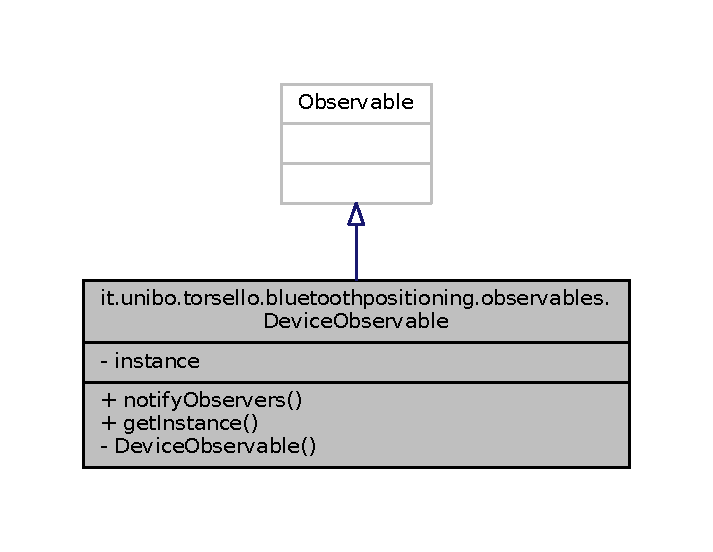
\includegraphics[width=342pt]{classit_1_1unibo_1_1torsello_1_1bluetoothpositioning_1_1observables_1_1DeviceObservable__inherit__graph}
\end{center}
\end{figure}


Diagramma di collaborazione per it.\+unibo.\+torsello.\+bluetoothpositioning.\+observables.\+Device\+Observable\+:
\nopagebreak
\begin{figure}[H]
\begin{center}
\leavevmode
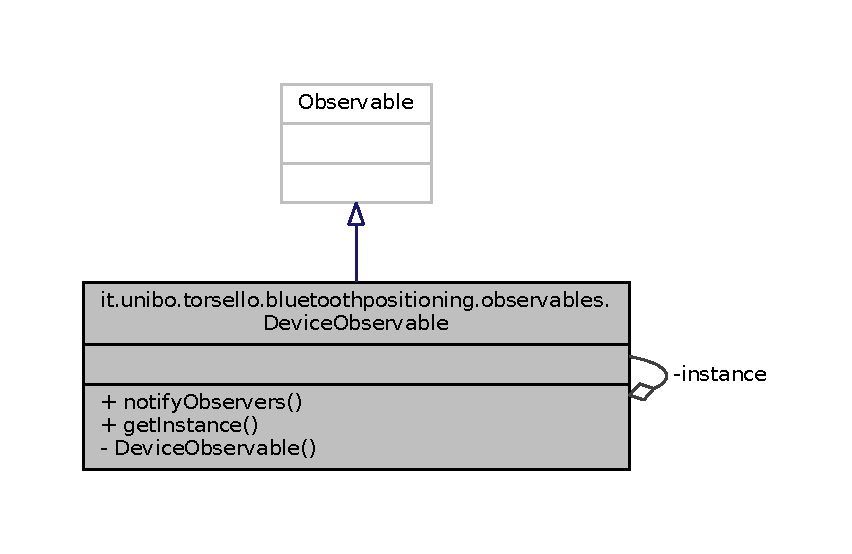
\includegraphics[width=350pt]{classit_1_1unibo_1_1torsello_1_1bluetoothpositioning_1_1observables_1_1DeviceObservable__coll__graph}
\end{center}
\end{figure}
\subsubsection*{Membri pubblici}
\begin{DoxyCompactItemize}
\item 
void \hyperlink{classit_1_1unibo_1_1torsello_1_1bluetoothpositioning_1_1observables_1_1DeviceObservable_aaf183e537e44cbd114c8eb76432da191_aaf183e537e44cbd114c8eb76432da191}{notify\+Observers} (Object data)
\end{DoxyCompactItemize}
\subsubsection*{Membri pubblici statici}
\begin{DoxyCompactItemize}
\item 
static \hyperlink{classit_1_1unibo_1_1torsello_1_1bluetoothpositioning_1_1observables_1_1DeviceObservable}{Device\+Observable} \hyperlink{classit_1_1unibo_1_1torsello_1_1bluetoothpositioning_1_1observables_1_1DeviceObservable_ab16792c5848440646624b2a41553954a_ab16792c5848440646624b2a41553954a}{get\+Instance} ()
\end{DoxyCompactItemize}
\subsubsection*{Membri privati}
\begin{DoxyCompactItemize}
\item 
\hyperlink{classit_1_1unibo_1_1torsello_1_1bluetoothpositioning_1_1observables_1_1DeviceObservable_afd89b681af0ee7708c8d3e830128cd2a_afd89b681af0ee7708c8d3e830128cd2a}{Device\+Observable} ()
\end{DoxyCompactItemize}
\subsubsection*{Attributi privati statici}
\begin{DoxyCompactItemize}
\item 
static \hyperlink{classit_1_1unibo_1_1torsello_1_1bluetoothpositioning_1_1observables_1_1DeviceObservable}{Device\+Observable} \hyperlink{classit_1_1unibo_1_1torsello_1_1bluetoothpositioning_1_1observables_1_1DeviceObservable_a43120f0ae1d6ae6c543219ec42df15e2_a43120f0ae1d6ae6c543219ec42df15e2}{instance} = new \hyperlink{classit_1_1unibo_1_1torsello_1_1bluetoothpositioning_1_1observables_1_1DeviceObservable}{Device\+Observable}()
\end{DoxyCompactItemize}


\subsubsection{Descrizione dettagliata}
Created by Federico Torsello. \href{mailto:federico.torsello@studio.unibo.it}{\tt federico.\+torsello@studio.\+unibo.\+it} 

\subsubsection{Documentazione dei costruttori e dei distruttori}
\hypertarget{classit_1_1unibo_1_1torsello_1_1bluetoothpositioning_1_1observables_1_1DeviceObservable_afd89b681af0ee7708c8d3e830128cd2a_afd89b681af0ee7708c8d3e830128cd2a}{}\label{classit_1_1unibo_1_1torsello_1_1bluetoothpositioning_1_1observables_1_1DeviceObservable_afd89b681af0ee7708c8d3e830128cd2a_afd89b681af0ee7708c8d3e830128cd2a} 
\index{it\+::unibo\+::torsello\+::bluetoothpositioning\+::observables\+::\+Device\+Observable@{it\+::unibo\+::torsello\+::bluetoothpositioning\+::observables\+::\+Device\+Observable}!Device\+Observable@{Device\+Observable}}
\index{Device\+Observable@{Device\+Observable}!it\+::unibo\+::torsello\+::bluetoothpositioning\+::observables\+::\+Device\+Observable@{it\+::unibo\+::torsello\+::bluetoothpositioning\+::observables\+::\+Device\+Observable}}
\paragraph{\texorpdfstring{Device\+Observable()}{DeviceObservable()}}
{\footnotesize\ttfamily it.\+unibo.\+torsello.\+bluetoothpositioning.\+observables.\+Device\+Observable.\+Device\+Observable (\begin{DoxyParamCaption}{ }\end{DoxyParamCaption})\hspace{0.3cm}{\ttfamily [private]}}


\begin{DoxyCode}
13                                \{
14         super();
15     \}
\end{DoxyCode}


\subsubsection{Documentazione delle funzioni membro}
\hypertarget{classit_1_1unibo_1_1torsello_1_1bluetoothpositioning_1_1observables_1_1DeviceObservable_ab16792c5848440646624b2a41553954a_ab16792c5848440646624b2a41553954a}{}\label{classit_1_1unibo_1_1torsello_1_1bluetoothpositioning_1_1observables_1_1DeviceObservable_ab16792c5848440646624b2a41553954a_ab16792c5848440646624b2a41553954a} 
\index{it\+::unibo\+::torsello\+::bluetoothpositioning\+::observables\+::\+Device\+Observable@{it\+::unibo\+::torsello\+::bluetoothpositioning\+::observables\+::\+Device\+Observable}!get\+Instance@{get\+Instance}}
\index{get\+Instance@{get\+Instance}!it\+::unibo\+::torsello\+::bluetoothpositioning\+::observables\+::\+Device\+Observable@{it\+::unibo\+::torsello\+::bluetoothpositioning\+::observables\+::\+Device\+Observable}}
\paragraph{\texorpdfstring{get\+Instance()}{getInstance()}}
{\footnotesize\ttfamily static \hyperlink{classit_1_1unibo_1_1torsello_1_1bluetoothpositioning_1_1observables_1_1DeviceObservable}{Device\+Observable} it.\+unibo.\+torsello.\+bluetoothpositioning.\+observables.\+Device\+Observable.\+get\+Instance (\begin{DoxyParamCaption}{ }\end{DoxyParamCaption})\hspace{0.3cm}{\ttfamily [static]}}


\begin{DoxyCode}
17                                                  \{
18         \textcolor{keywordflow}{return} \hyperlink{classit_1_1unibo_1_1torsello_1_1bluetoothpositioning_1_1observables_1_1DeviceObservable_a43120f0ae1d6ae6c543219ec42df15e2_a43120f0ae1d6ae6c543219ec42df15e2}{instance};
19     \}
\end{DoxyCode}
\hypertarget{classit_1_1unibo_1_1torsello_1_1bluetoothpositioning_1_1observables_1_1DeviceObservable_aaf183e537e44cbd114c8eb76432da191_aaf183e537e44cbd114c8eb76432da191}{}\label{classit_1_1unibo_1_1torsello_1_1bluetoothpositioning_1_1observables_1_1DeviceObservable_aaf183e537e44cbd114c8eb76432da191_aaf183e537e44cbd114c8eb76432da191} 
\index{it\+::unibo\+::torsello\+::bluetoothpositioning\+::observables\+::\+Device\+Observable@{it\+::unibo\+::torsello\+::bluetoothpositioning\+::observables\+::\+Device\+Observable}!notify\+Observers@{notify\+Observers}}
\index{notify\+Observers@{notify\+Observers}!it\+::unibo\+::torsello\+::bluetoothpositioning\+::observables\+::\+Device\+Observable@{it\+::unibo\+::torsello\+::bluetoothpositioning\+::observables\+::\+Device\+Observable}}
\paragraph{\texorpdfstring{notify\+Observers()}{notifyObservers()}}
{\footnotesize\ttfamily void it.\+unibo.\+torsello.\+bluetoothpositioning.\+observables.\+Device\+Observable.\+notify\+Observers (\begin{DoxyParamCaption}\item[{Object}]{data }\end{DoxyParamCaption})}


\begin{DoxyCode}
22                                              \{
23         setChanged();
24         super.notifyObservers(data);
25     \}
\end{DoxyCode}


\subsubsection{Documentazione dei membri dato}
\hypertarget{classit_1_1unibo_1_1torsello_1_1bluetoothpositioning_1_1observables_1_1DeviceObservable_a43120f0ae1d6ae6c543219ec42df15e2_a43120f0ae1d6ae6c543219ec42df15e2}{}\label{classit_1_1unibo_1_1torsello_1_1bluetoothpositioning_1_1observables_1_1DeviceObservable_a43120f0ae1d6ae6c543219ec42df15e2_a43120f0ae1d6ae6c543219ec42df15e2} 
\index{it\+::unibo\+::torsello\+::bluetoothpositioning\+::observables\+::\+Device\+Observable@{it\+::unibo\+::torsello\+::bluetoothpositioning\+::observables\+::\+Device\+Observable}!instance@{instance}}
\index{instance@{instance}!it\+::unibo\+::torsello\+::bluetoothpositioning\+::observables\+::\+Device\+Observable@{it\+::unibo\+::torsello\+::bluetoothpositioning\+::observables\+::\+Device\+Observable}}
\paragraph{\texorpdfstring{instance}{instance}}
{\footnotesize\ttfamily \hyperlink{classit_1_1unibo_1_1torsello_1_1bluetoothpositioning_1_1observables_1_1DeviceObservable}{Device\+Observable} it.\+unibo.\+torsello.\+bluetoothpositioning.\+observables.\+Device\+Observable.\+instance = new \hyperlink{classit_1_1unibo_1_1torsello_1_1bluetoothpositioning_1_1observables_1_1DeviceObservable}{Device\+Observable}()\hspace{0.3cm}{\ttfamily [static]}, {\ttfamily [private]}}



La documentazione per questa classe è stata generata a partire dal seguente file\+:\begin{DoxyCompactItemize}
\item 
\hyperlink{DeviceObservable_8java}{Device\+Observable.\+java}\end{DoxyCompactItemize}

\hypertarget{classit_1_1unibo_1_1torsello_1_1bluetoothpositioning_1_1adapter_1_1DeviceCardViewAdapter_1_1DeviceViewHolder}{}\subsection{Riferimenti per la classe it.\+unibo.\+torsello.\+bluetoothpositioning.\+adapter.\+Device\+Card\+View\+Adapter.\+Device\+View\+Holder}
\label{classit_1_1unibo_1_1torsello_1_1bluetoothpositioning_1_1adapter_1_1DeviceCardViewAdapter_1_1DeviceViewHolder}\index{it.\+unibo.\+torsello.\+bluetoothpositioning.\+adapter.\+Device\+Card\+View\+Adapter.\+Device\+View\+Holder@{it.\+unibo.\+torsello.\+bluetoothpositioning.\+adapter.\+Device\+Card\+View\+Adapter.\+Device\+View\+Holder}}


Diagramma delle classi per it.\+unibo.\+torsello.\+bluetoothpositioning.\+adapter.\+Device\+Card\+View\+Adapter.\+Device\+View\+Holder
\nopagebreak
\begin{figure}[H]
\begin{center}
\leavevmode
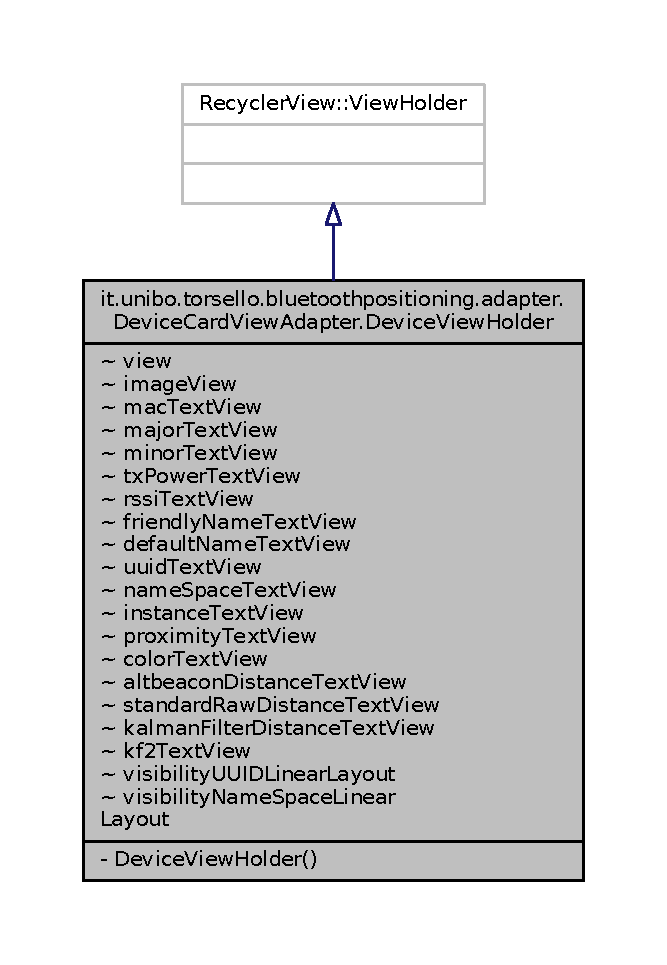
\includegraphics[width=320pt]{classit_1_1unibo_1_1torsello_1_1bluetoothpositioning_1_1adapter_1_1DeviceCardViewAdapter_1_1DeviceViewHolder__inherit__graph}
\end{center}
\end{figure}


Diagramma di collaborazione per it.\+unibo.\+torsello.\+bluetoothpositioning.\+adapter.\+Device\+Card\+View\+Adapter.\+Device\+View\+Holder\+:
\nopagebreak
\begin{figure}[H]
\begin{center}
\leavevmode
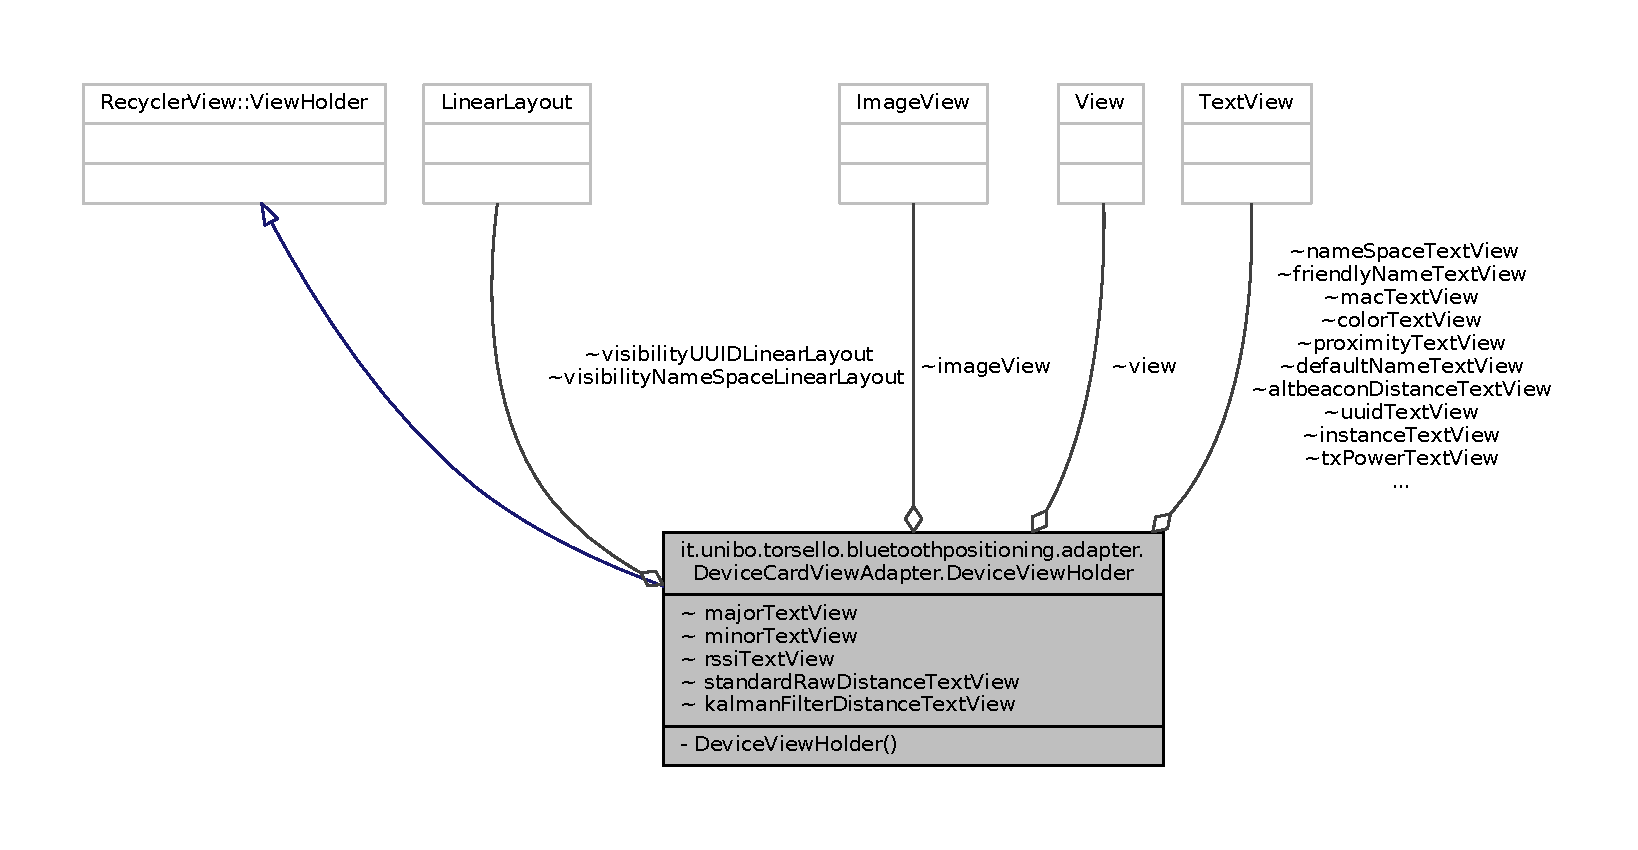
\includegraphics[width=350pt]{classit_1_1unibo_1_1torsello_1_1bluetoothpositioning_1_1adapter_1_1DeviceCardViewAdapter_1_1DeviceViewHolder__coll__graph}
\end{center}
\end{figure}
\subsubsection*{Attributi con visibilità di package}
\begin{DoxyCompactItemize}
\item 
View \hyperlink{classit_1_1unibo_1_1torsello_1_1bluetoothpositioning_1_1adapter_1_1DeviceCardViewAdapter_1_1DeviceViewHolder_a4aa2da965bbcbc091ae913aea1e0a5cd_a4aa2da965bbcbc091ae913aea1e0a5cd}{view}
\item 
Image\+View \hyperlink{classit_1_1unibo_1_1torsello_1_1bluetoothpositioning_1_1adapter_1_1DeviceCardViewAdapter_1_1DeviceViewHolder_a347a5569ea11fee0f721d0853ba1383a_a347a5569ea11fee0f721d0853ba1383a}{image\+View}
\item 
Text\+View \hyperlink{classit_1_1unibo_1_1torsello_1_1bluetoothpositioning_1_1adapter_1_1DeviceCardViewAdapter_1_1DeviceViewHolder_af70da9970d914ec47f1a19c4b46d6fe0_af70da9970d914ec47f1a19c4b46d6fe0}{mac\+Text\+View}
\item 
Text\+View \hyperlink{classit_1_1unibo_1_1torsello_1_1bluetoothpositioning_1_1adapter_1_1DeviceCardViewAdapter_1_1DeviceViewHolder_ab436c91c0fac49199cc1a275ce2911e0_ab436c91c0fac49199cc1a275ce2911e0}{major\+Text\+View}
\item 
Text\+View \hyperlink{classit_1_1unibo_1_1torsello_1_1bluetoothpositioning_1_1adapter_1_1DeviceCardViewAdapter_1_1DeviceViewHolder_ac23ff2b20dcea8f3847023fbe8a6ca00_ac23ff2b20dcea8f3847023fbe8a6ca00}{minor\+Text\+View}
\item 
Text\+View \hyperlink{classit_1_1unibo_1_1torsello_1_1bluetoothpositioning_1_1adapter_1_1DeviceCardViewAdapter_1_1DeviceViewHolder_aefed6d7b85f2616d61a6d5eb3bdc5b42_aefed6d7b85f2616d61a6d5eb3bdc5b42}{tx\+Power\+Text\+View}
\item 
Text\+View \hyperlink{classit_1_1unibo_1_1torsello_1_1bluetoothpositioning_1_1adapter_1_1DeviceCardViewAdapter_1_1DeviceViewHolder_a5a1945d4212a1aff801998aecdb7b89e_a5a1945d4212a1aff801998aecdb7b89e}{rssi\+Text\+View}
\item 
Text\+View \hyperlink{classit_1_1unibo_1_1torsello_1_1bluetoothpositioning_1_1adapter_1_1DeviceCardViewAdapter_1_1DeviceViewHolder_abd00e1fa8a2d2f6c46e6c43d59c43c09_abd00e1fa8a2d2f6c46e6c43d59c43c09}{friendly\+Name\+Text\+View}
\item 
Text\+View \hyperlink{classit_1_1unibo_1_1torsello_1_1bluetoothpositioning_1_1adapter_1_1DeviceCardViewAdapter_1_1DeviceViewHolder_a26c7f741a315cf43fca6570375dca93a_a26c7f741a315cf43fca6570375dca93a}{default\+Name\+Text\+View}
\item 
Text\+View \hyperlink{classit_1_1unibo_1_1torsello_1_1bluetoothpositioning_1_1adapter_1_1DeviceCardViewAdapter_1_1DeviceViewHolder_ac4c704d6332705288b277bddcc922eb3_ac4c704d6332705288b277bddcc922eb3}{uuid\+Text\+View}
\item 
Text\+View \hyperlink{classit_1_1unibo_1_1torsello_1_1bluetoothpositioning_1_1adapter_1_1DeviceCardViewAdapter_1_1DeviceViewHolder_a7c487cde57093a878929990ba61d173c_a7c487cde57093a878929990ba61d173c}{name\+Space\+Text\+View}
\item 
Text\+View \hyperlink{classit_1_1unibo_1_1torsello_1_1bluetoothpositioning_1_1adapter_1_1DeviceCardViewAdapter_1_1DeviceViewHolder_afd46ff4d479b502963dd9630efc9f177_afd46ff4d479b502963dd9630efc9f177}{instance\+Text\+View}
\item 
Text\+View \hyperlink{classit_1_1unibo_1_1torsello_1_1bluetoothpositioning_1_1adapter_1_1DeviceCardViewAdapter_1_1DeviceViewHolder_a1ddd659d463c9b409b4a9df663e0fa05_a1ddd659d463c9b409b4a9df663e0fa05}{proximity\+Text\+View}
\item 
Text\+View \hyperlink{classit_1_1unibo_1_1torsello_1_1bluetoothpositioning_1_1adapter_1_1DeviceCardViewAdapter_1_1DeviceViewHolder_a13b19031bd21f4beee3809d4917429de_a13b19031bd21f4beee3809d4917429de}{color\+Text\+View}
\item 
Text\+View \hyperlink{classit_1_1unibo_1_1torsello_1_1bluetoothpositioning_1_1adapter_1_1DeviceCardViewAdapter_1_1DeviceViewHolder_ac6ec3f5e17e0feda143c7883d6115334_ac6ec3f5e17e0feda143c7883d6115334}{altbeacon\+Distance\+Text\+View}
\item 
Text\+View \hyperlink{classit_1_1unibo_1_1torsello_1_1bluetoothpositioning_1_1adapter_1_1DeviceCardViewAdapter_1_1DeviceViewHolder_a1465eea620da435cda3037fefd715a90_a1465eea620da435cda3037fefd715a90}{standard\+Raw\+Distance\+Text\+View}
\item 
Text\+View \hyperlink{classit_1_1unibo_1_1torsello_1_1bluetoothpositioning_1_1adapter_1_1DeviceCardViewAdapter_1_1DeviceViewHolder_a1e0cad4bb83fa3f733d84ca6decd50c4_a1e0cad4bb83fa3f733d84ca6decd50c4}{kalman\+Filter\+Distance\+Text\+View}
\item 
Linear\+Layout \hyperlink{classit_1_1unibo_1_1torsello_1_1bluetoothpositioning_1_1adapter_1_1DeviceCardViewAdapter_1_1DeviceViewHolder_a72e4e3a233aa8cff4c3fe8e28a156095_a72e4e3a233aa8cff4c3fe8e28a156095}{visibility\+U\+U\+I\+D\+Linear\+Layout}
\item 
Linear\+Layout \hyperlink{classit_1_1unibo_1_1torsello_1_1bluetoothpositioning_1_1adapter_1_1DeviceCardViewAdapter_1_1DeviceViewHolder_aa3b69bc26e552aef6c18acb40e991d27_aa3b69bc26e552aef6c18acb40e991d27}{visibility\+Name\+Space\+Linear\+Layout}
\end{DoxyCompactItemize}
\subsubsection*{Membri privati}
\begin{DoxyCompactItemize}
\item 
\hyperlink{classit_1_1unibo_1_1torsello_1_1bluetoothpositioning_1_1adapter_1_1DeviceCardViewAdapter_1_1DeviceViewHolder_a75016d2a0df1fc991a5a6aed86b776d2_a75016d2a0df1fc991a5a6aed86b776d2}{Device\+View\+Holder} (View \hyperlink{classit_1_1unibo_1_1torsello_1_1bluetoothpositioning_1_1adapter_1_1DeviceCardViewAdapter_1_1DeviceViewHolder_a4aa2da965bbcbc091ae913aea1e0a5cd_a4aa2da965bbcbc091ae913aea1e0a5cd}{view})
\end{DoxyCompactItemize}


\subsubsection{Documentazione dei costruttori e dei distruttori}
\hypertarget{classit_1_1unibo_1_1torsello_1_1bluetoothpositioning_1_1adapter_1_1DeviceCardViewAdapter_1_1DeviceViewHolder_a75016d2a0df1fc991a5a6aed86b776d2_a75016d2a0df1fc991a5a6aed86b776d2}{}\label{classit_1_1unibo_1_1torsello_1_1bluetoothpositioning_1_1adapter_1_1DeviceCardViewAdapter_1_1DeviceViewHolder_a75016d2a0df1fc991a5a6aed86b776d2_a75016d2a0df1fc991a5a6aed86b776d2} 
\index{it\+::unibo\+::torsello\+::bluetoothpositioning\+::adapter\+::\+Device\+Card\+View\+Adapter\+::\+Device\+View\+Holder@{it\+::unibo\+::torsello\+::bluetoothpositioning\+::adapter\+::\+Device\+Card\+View\+Adapter\+::\+Device\+View\+Holder}!Device\+View\+Holder@{Device\+View\+Holder}}
\index{Device\+View\+Holder@{Device\+View\+Holder}!it\+::unibo\+::torsello\+::bluetoothpositioning\+::adapter\+::\+Device\+Card\+View\+Adapter\+::\+Device\+View\+Holder@{it\+::unibo\+::torsello\+::bluetoothpositioning\+::adapter\+::\+Device\+Card\+View\+Adapter\+::\+Device\+View\+Holder}}
\paragraph{\texorpdfstring{Device\+View\+Holder()}{DeviceViewHolder()}}
{\footnotesize\ttfamily it.\+unibo.\+torsello.\+bluetoothpositioning.\+adapter.\+Device\+Card\+View\+Adapter.\+Device\+View\+Holder.\+Device\+View\+Holder (\begin{DoxyParamCaption}\item[{View}]{view }\end{DoxyParamCaption})\hspace{0.3cm}{\ttfamily [private]}}


\begin{DoxyCode}
250                                             \{
251 
252             super(\hyperlink{classit_1_1unibo_1_1torsello_1_1bluetoothpositioning_1_1adapter_1_1DeviceCardViewAdapter_1_1DeviceViewHolder_a4aa2da965bbcbc091ae913aea1e0a5cd_a4aa2da965bbcbc091ae913aea1e0a5cd}{view});
253             this.\hyperlink{classit_1_1unibo_1_1torsello_1_1bluetoothpositioning_1_1adapter_1_1DeviceCardViewAdapter_1_1DeviceViewHolder_a4aa2da965bbcbc091ae913aea1e0a5cd_a4aa2da965bbcbc091ae913aea1e0a5cd}{view} = \hyperlink{classit_1_1unibo_1_1torsello_1_1bluetoothpositioning_1_1adapter_1_1DeviceCardViewAdapter_1_1DeviceViewHolder_a4aa2da965bbcbc091ae913aea1e0a5cd_a4aa2da965bbcbc091ae913aea1e0a5cd}{view};
254             \hyperlink{classit_1_1unibo_1_1torsello_1_1bluetoothpositioning_1_1adapter_1_1DeviceCardViewAdapter_1_1DeviceViewHolder_a347a5569ea11fee0f721d0853ba1383a_a347a5569ea11fee0f721d0853ba1383a}{imageView} = (ImageView) \hyperlink{classit_1_1unibo_1_1torsello_1_1bluetoothpositioning_1_1adapter_1_1DeviceCardViewAdapter_1_1DeviceViewHolder_a4aa2da965bbcbc091ae913aea1e0a5cd_a4aa2da965bbcbc091ae913aea1e0a5cd}{view}.findViewById(R.id.imageBeacon);
255             \hyperlink{classit_1_1unibo_1_1torsello_1_1bluetoothpositioning_1_1adapter_1_1DeviceCardViewAdapter_1_1DeviceViewHolder_a26c7f741a315cf43fca6570375dca93a_a26c7f741a315cf43fca6570375dca93a}{defaultNameTextView} = (TextView) \hyperlink{classit_1_1unibo_1_1torsello_1_1bluetoothpositioning_1_1adapter_1_1DeviceCardViewAdapter_1_1DeviceViewHolder_a4aa2da965bbcbc091ae913aea1e0a5cd_a4aa2da965bbcbc091ae913aea1e0a5cd}{view}.findViewById(R.id.
      value\_default\_name);
256             \hyperlink{classit_1_1unibo_1_1torsello_1_1bluetoothpositioning_1_1adapter_1_1DeviceCardViewAdapter_1_1DeviceViewHolder_abd00e1fa8a2d2f6c46e6c43d59c43c09_abd00e1fa8a2d2f6c46e6c43d59c43c09}{friendlyNameTextView} = (TextView) \hyperlink{classit_1_1unibo_1_1torsello_1_1bluetoothpositioning_1_1adapter_1_1DeviceCardViewAdapter_1_1DeviceViewHolder_a4aa2da965bbcbc091ae913aea1e0a5cd_a4aa2da965bbcbc091ae913aea1e0a5cd}{view}.findViewById(R.id.
      value\_friendly\_name);
257             \hyperlink{classit_1_1unibo_1_1torsello_1_1bluetoothpositioning_1_1adapter_1_1DeviceCardViewAdapter_1_1DeviceViewHolder_af70da9970d914ec47f1a19c4b46d6fe0_af70da9970d914ec47f1a19c4b46d6fe0}{macTextView} = (TextView) \hyperlink{classit_1_1unibo_1_1torsello_1_1bluetoothpositioning_1_1adapter_1_1DeviceCardViewAdapter_1_1DeviceViewHolder_a4aa2da965bbcbc091ae913aea1e0a5cd_a4aa2da965bbcbc091ae913aea1e0a5cd}{view}.findViewById(R.id.value\_mac\_address);
258             \hyperlink{classit_1_1unibo_1_1torsello_1_1bluetoothpositioning_1_1adapter_1_1DeviceCardViewAdapter_1_1DeviceViewHolder_ab436c91c0fac49199cc1a275ce2911e0_ab436c91c0fac49199cc1a275ce2911e0}{majorTextView} = (TextView) \hyperlink{classit_1_1unibo_1_1torsello_1_1bluetoothpositioning_1_1adapter_1_1DeviceCardViewAdapter_1_1DeviceViewHolder_a4aa2da965bbcbc091ae913aea1e0a5cd_a4aa2da965bbcbc091ae913aea1e0a5cd}{view}.findViewById(R.id.value\_major);
259             \hyperlink{classit_1_1unibo_1_1torsello_1_1bluetoothpositioning_1_1adapter_1_1DeviceCardViewAdapter_1_1DeviceViewHolder_ac23ff2b20dcea8f3847023fbe8a6ca00_ac23ff2b20dcea8f3847023fbe8a6ca00}{minorTextView} = (TextView) \hyperlink{classit_1_1unibo_1_1torsello_1_1bluetoothpositioning_1_1adapter_1_1DeviceCardViewAdapter_1_1DeviceViewHolder_a4aa2da965bbcbc091ae913aea1e0a5cd_a4aa2da965bbcbc091ae913aea1e0a5cd}{view}.findViewById(R.id.value\_minor);
260             \hyperlink{classit_1_1unibo_1_1torsello_1_1bluetoothpositioning_1_1adapter_1_1DeviceCardViewAdapter_1_1DeviceViewHolder_aefed6d7b85f2616d61a6d5eb3bdc5b42_aefed6d7b85f2616d61a6d5eb3bdc5b42}{txPowerTextView} = (TextView) \hyperlink{classit_1_1unibo_1_1torsello_1_1bluetoothpositioning_1_1adapter_1_1DeviceCardViewAdapter_1_1DeviceViewHolder_a4aa2da965bbcbc091ae913aea1e0a5cd_a4aa2da965bbcbc091ae913aea1e0a5cd}{view}.findViewById(R.id.value\_power);
261             \hyperlink{classit_1_1unibo_1_1torsello_1_1bluetoothpositioning_1_1adapter_1_1DeviceCardViewAdapter_1_1DeviceViewHolder_a5a1945d4212a1aff801998aecdb7b89e_a5a1945d4212a1aff801998aecdb7b89e}{rssiTextView} = (TextView) \hyperlink{classit_1_1unibo_1_1torsello_1_1bluetoothpositioning_1_1adapter_1_1DeviceCardViewAdapter_1_1DeviceViewHolder_a4aa2da965bbcbc091ae913aea1e0a5cd_a4aa2da965bbcbc091ae913aea1e0a5cd}{view}.findViewById(R.id.value\_rssi);
262             \hyperlink{classit_1_1unibo_1_1torsello_1_1bluetoothpositioning_1_1adapter_1_1DeviceCardViewAdapter_1_1DeviceViewHolder_ac4c704d6332705288b277bddcc922eb3_ac4c704d6332705288b277bddcc922eb3}{uuidTextView} = (TextView) \hyperlink{classit_1_1unibo_1_1torsello_1_1bluetoothpositioning_1_1adapter_1_1DeviceCardViewAdapter_1_1DeviceViewHolder_a4aa2da965bbcbc091ae913aea1e0a5cd_a4aa2da965bbcbc091ae913aea1e0a5cd}{view}.findViewById(R.id.value\_uuid);
263             \hyperlink{classit_1_1unibo_1_1torsello_1_1bluetoothpositioning_1_1adapter_1_1DeviceCardViewAdapter_1_1DeviceViewHolder_a7c487cde57093a878929990ba61d173c_a7c487cde57093a878929990ba61d173c}{nameSpaceTextView} = (TextView) \hyperlink{classit_1_1unibo_1_1torsello_1_1bluetoothpositioning_1_1adapter_1_1DeviceCardViewAdapter_1_1DeviceViewHolder_a4aa2da965bbcbc091ae913aea1e0a5cd_a4aa2da965bbcbc091ae913aea1e0a5cd}{view}.findViewById(R.id.value\_name\_space);
264             \hyperlink{classit_1_1unibo_1_1torsello_1_1bluetoothpositioning_1_1adapter_1_1DeviceCardViewAdapter_1_1DeviceViewHolder_a1ddd659d463c9b409b4a9df663e0fa05_a1ddd659d463c9b409b4a9df663e0fa05}{proximityTextView} = (TextView) \hyperlink{classit_1_1unibo_1_1torsello_1_1bluetoothpositioning_1_1adapter_1_1DeviceCardViewAdapter_1_1DeviceViewHolder_a4aa2da965bbcbc091ae913aea1e0a5cd_a4aa2da965bbcbc091ae913aea1e0a5cd}{view}.findViewById(R.id.value\_proximity);
265             \hyperlink{classit_1_1unibo_1_1torsello_1_1bluetoothpositioning_1_1adapter_1_1DeviceCardViewAdapter_1_1DeviceViewHolder_afd46ff4d479b502963dd9630efc9f177_afd46ff4d479b502963dd9630efc9f177}{instanceTextView} = (TextView) \hyperlink{classit_1_1unibo_1_1torsello_1_1bluetoothpositioning_1_1adapter_1_1DeviceCardViewAdapter_1_1DeviceViewHolder_a4aa2da965bbcbc091ae913aea1e0a5cd_a4aa2da965bbcbc091ae913aea1e0a5cd}{view}.findViewById(R.id.value\_instance);
266             \hyperlink{classit_1_1unibo_1_1torsello_1_1bluetoothpositioning_1_1adapter_1_1DeviceCardViewAdapter_1_1DeviceViewHolder_a13b19031bd21f4beee3809d4917429de_a13b19031bd21f4beee3809d4917429de}{colorTextView} = (TextView) \hyperlink{classit_1_1unibo_1_1torsello_1_1bluetoothpositioning_1_1adapter_1_1DeviceCardViewAdapter_1_1DeviceViewHolder_a4aa2da965bbcbc091ae913aea1e0a5cd_a4aa2da965bbcbc091ae913aea1e0a5cd}{view}.findViewById(R.id.value\_color);
267 
268             \hyperlink{classit_1_1unibo_1_1torsello_1_1bluetoothpositioning_1_1adapter_1_1DeviceCardViewAdapter_1_1DeviceViewHolder_ac6ec3f5e17e0feda143c7883d6115334_ac6ec3f5e17e0feda143c7883d6115334}{altbeaconDistanceTextView} = (TextView) \hyperlink{classit_1_1unibo_1_1torsello_1_1bluetoothpositioning_1_1adapter_1_1DeviceCardViewAdapter_1_1DeviceViewHolder_a4aa2da965bbcbc091ae913aea1e0a5cd_a4aa2da965bbcbc091ae913aea1e0a5cd}{view}.findViewById(R.id.
      value\_altbeacon\_distance);
269             \hyperlink{classit_1_1unibo_1_1torsello_1_1bluetoothpositioning_1_1adapter_1_1DeviceCardViewAdapter_1_1DeviceViewHolder_a1e0cad4bb83fa3f733d84ca6decd50c4_a1e0cad4bb83fa3f733d84ca6decd50c4}{kalmanFilterDistanceTextView} = (TextView) 
      \hyperlink{classit_1_1unibo_1_1torsello_1_1bluetoothpositioning_1_1adapter_1_1DeviceCardViewAdapter_1_1DeviceViewHolder_a4aa2da965bbcbc091ae913aea1e0a5cd_a4aa2da965bbcbc091ae913aea1e0a5cd}{view}.findViewById(R.id.value\_kalman\_filter\_distance);
270             \hyperlink{classit_1_1unibo_1_1torsello_1_1bluetoothpositioning_1_1adapter_1_1DeviceCardViewAdapter_1_1DeviceViewHolder_a1465eea620da435cda3037fefd715a90_a1465eea620da435cda3037fefd715a90}{standardRawDistanceTextView} = (TextView) 
      \hyperlink{classit_1_1unibo_1_1torsello_1_1bluetoothpositioning_1_1adapter_1_1DeviceCardViewAdapter_1_1DeviceViewHolder_a4aa2da965bbcbc091ae913aea1e0a5cd_a4aa2da965bbcbc091ae913aea1e0a5cd}{view}.findViewById(R.id.value\_standard\_raw\_distance);
271 
272             \hyperlink{classit_1_1unibo_1_1torsello_1_1bluetoothpositioning_1_1adapter_1_1DeviceCardViewAdapter_1_1DeviceViewHolder_a72e4e3a233aa8cff4c3fe8e28a156095_a72e4e3a233aa8cff4c3fe8e28a156095}{visibilityUUIDLinearLayout} = (LinearLayout) 
      \hyperlink{classit_1_1unibo_1_1torsello_1_1bluetoothpositioning_1_1adapter_1_1DeviceCardViewAdapter_1_1DeviceViewHolder_a4aa2da965bbcbc091ae913aea1e0a5cd_a4aa2da965bbcbc091ae913aea1e0a5cd}{view}.findViewById(R.id.visibility\_uuid\_minor\_major\_nmb);
273             \hyperlink{classit_1_1unibo_1_1torsello_1_1bluetoothpositioning_1_1adapter_1_1DeviceCardViewAdapter_1_1DeviceViewHolder_aa3b69bc26e552aef6c18acb40e991d27_aa3b69bc26e552aef6c18acb40e991d27}{visibilityNameSpaceLinearLayout} = (LinearLayout) 
      \hyperlink{classit_1_1unibo_1_1torsello_1_1bluetoothpositioning_1_1adapter_1_1DeviceCardViewAdapter_1_1DeviceViewHolder_a4aa2da965bbcbc091ae913aea1e0a5cd_a4aa2da965bbcbc091ae913aea1e0a5cd}{view}.findViewById(R.id.visibilityNameSpace\_Instance);
274         \}
\end{DoxyCode}


\subsubsection{Documentazione dei membri dato}
\hypertarget{classit_1_1unibo_1_1torsello_1_1bluetoothpositioning_1_1adapter_1_1DeviceCardViewAdapter_1_1DeviceViewHolder_ac6ec3f5e17e0feda143c7883d6115334_ac6ec3f5e17e0feda143c7883d6115334}{}\label{classit_1_1unibo_1_1torsello_1_1bluetoothpositioning_1_1adapter_1_1DeviceCardViewAdapter_1_1DeviceViewHolder_ac6ec3f5e17e0feda143c7883d6115334_ac6ec3f5e17e0feda143c7883d6115334} 
\index{it\+::unibo\+::torsello\+::bluetoothpositioning\+::adapter\+::\+Device\+Card\+View\+Adapter\+::\+Device\+View\+Holder@{it\+::unibo\+::torsello\+::bluetoothpositioning\+::adapter\+::\+Device\+Card\+View\+Adapter\+::\+Device\+View\+Holder}!altbeacon\+Distance\+Text\+View@{altbeacon\+Distance\+Text\+View}}
\index{altbeacon\+Distance\+Text\+View@{altbeacon\+Distance\+Text\+View}!it\+::unibo\+::torsello\+::bluetoothpositioning\+::adapter\+::\+Device\+Card\+View\+Adapter\+::\+Device\+View\+Holder@{it\+::unibo\+::torsello\+::bluetoothpositioning\+::adapter\+::\+Device\+Card\+View\+Adapter\+::\+Device\+View\+Holder}}
\paragraph{\texorpdfstring{altbeacon\+Distance\+Text\+View}{altbeaconDistanceTextView}}
{\footnotesize\ttfamily Text\+View it.\+unibo.\+torsello.\+bluetoothpositioning.\+adapter.\+Device\+Card\+View\+Adapter.\+Device\+View\+Holder.\+altbeacon\+Distance\+Text\+View\hspace{0.3cm}{\ttfamily [package]}}

\hypertarget{classit_1_1unibo_1_1torsello_1_1bluetoothpositioning_1_1adapter_1_1DeviceCardViewAdapter_1_1DeviceViewHolder_a13b19031bd21f4beee3809d4917429de_a13b19031bd21f4beee3809d4917429de}{}\label{classit_1_1unibo_1_1torsello_1_1bluetoothpositioning_1_1adapter_1_1DeviceCardViewAdapter_1_1DeviceViewHolder_a13b19031bd21f4beee3809d4917429de_a13b19031bd21f4beee3809d4917429de} 
\index{it\+::unibo\+::torsello\+::bluetoothpositioning\+::adapter\+::\+Device\+Card\+View\+Adapter\+::\+Device\+View\+Holder@{it\+::unibo\+::torsello\+::bluetoothpositioning\+::adapter\+::\+Device\+Card\+View\+Adapter\+::\+Device\+View\+Holder}!color\+Text\+View@{color\+Text\+View}}
\index{color\+Text\+View@{color\+Text\+View}!it\+::unibo\+::torsello\+::bluetoothpositioning\+::adapter\+::\+Device\+Card\+View\+Adapter\+::\+Device\+View\+Holder@{it\+::unibo\+::torsello\+::bluetoothpositioning\+::adapter\+::\+Device\+Card\+View\+Adapter\+::\+Device\+View\+Holder}}
\paragraph{\texorpdfstring{color\+Text\+View}{colorTextView}}
{\footnotesize\ttfamily Text\+View it.\+unibo.\+torsello.\+bluetoothpositioning.\+adapter.\+Device\+Card\+View\+Adapter.\+Device\+View\+Holder.\+color\+Text\+View\hspace{0.3cm}{\ttfamily [package]}}

\hypertarget{classit_1_1unibo_1_1torsello_1_1bluetoothpositioning_1_1adapter_1_1DeviceCardViewAdapter_1_1DeviceViewHolder_a26c7f741a315cf43fca6570375dca93a_a26c7f741a315cf43fca6570375dca93a}{}\label{classit_1_1unibo_1_1torsello_1_1bluetoothpositioning_1_1adapter_1_1DeviceCardViewAdapter_1_1DeviceViewHolder_a26c7f741a315cf43fca6570375dca93a_a26c7f741a315cf43fca6570375dca93a} 
\index{it\+::unibo\+::torsello\+::bluetoothpositioning\+::adapter\+::\+Device\+Card\+View\+Adapter\+::\+Device\+View\+Holder@{it\+::unibo\+::torsello\+::bluetoothpositioning\+::adapter\+::\+Device\+Card\+View\+Adapter\+::\+Device\+View\+Holder}!default\+Name\+Text\+View@{default\+Name\+Text\+View}}
\index{default\+Name\+Text\+View@{default\+Name\+Text\+View}!it\+::unibo\+::torsello\+::bluetoothpositioning\+::adapter\+::\+Device\+Card\+View\+Adapter\+::\+Device\+View\+Holder@{it\+::unibo\+::torsello\+::bluetoothpositioning\+::adapter\+::\+Device\+Card\+View\+Adapter\+::\+Device\+View\+Holder}}
\paragraph{\texorpdfstring{default\+Name\+Text\+View}{defaultNameTextView}}
{\footnotesize\ttfamily Text\+View it.\+unibo.\+torsello.\+bluetoothpositioning.\+adapter.\+Device\+Card\+View\+Adapter.\+Device\+View\+Holder.\+default\+Name\+Text\+View\hspace{0.3cm}{\ttfamily [package]}}

\hypertarget{classit_1_1unibo_1_1torsello_1_1bluetoothpositioning_1_1adapter_1_1DeviceCardViewAdapter_1_1DeviceViewHolder_abd00e1fa8a2d2f6c46e6c43d59c43c09_abd00e1fa8a2d2f6c46e6c43d59c43c09}{}\label{classit_1_1unibo_1_1torsello_1_1bluetoothpositioning_1_1adapter_1_1DeviceCardViewAdapter_1_1DeviceViewHolder_abd00e1fa8a2d2f6c46e6c43d59c43c09_abd00e1fa8a2d2f6c46e6c43d59c43c09} 
\index{it\+::unibo\+::torsello\+::bluetoothpositioning\+::adapter\+::\+Device\+Card\+View\+Adapter\+::\+Device\+View\+Holder@{it\+::unibo\+::torsello\+::bluetoothpositioning\+::adapter\+::\+Device\+Card\+View\+Adapter\+::\+Device\+View\+Holder}!friendly\+Name\+Text\+View@{friendly\+Name\+Text\+View}}
\index{friendly\+Name\+Text\+View@{friendly\+Name\+Text\+View}!it\+::unibo\+::torsello\+::bluetoothpositioning\+::adapter\+::\+Device\+Card\+View\+Adapter\+::\+Device\+View\+Holder@{it\+::unibo\+::torsello\+::bluetoothpositioning\+::adapter\+::\+Device\+Card\+View\+Adapter\+::\+Device\+View\+Holder}}
\paragraph{\texorpdfstring{friendly\+Name\+Text\+View}{friendlyNameTextView}}
{\footnotesize\ttfamily Text\+View it.\+unibo.\+torsello.\+bluetoothpositioning.\+adapter.\+Device\+Card\+View\+Adapter.\+Device\+View\+Holder.\+friendly\+Name\+Text\+View\hspace{0.3cm}{\ttfamily [package]}}

\hypertarget{classit_1_1unibo_1_1torsello_1_1bluetoothpositioning_1_1adapter_1_1DeviceCardViewAdapter_1_1DeviceViewHolder_a347a5569ea11fee0f721d0853ba1383a_a347a5569ea11fee0f721d0853ba1383a}{}\label{classit_1_1unibo_1_1torsello_1_1bluetoothpositioning_1_1adapter_1_1DeviceCardViewAdapter_1_1DeviceViewHolder_a347a5569ea11fee0f721d0853ba1383a_a347a5569ea11fee0f721d0853ba1383a} 
\index{it\+::unibo\+::torsello\+::bluetoothpositioning\+::adapter\+::\+Device\+Card\+View\+Adapter\+::\+Device\+View\+Holder@{it\+::unibo\+::torsello\+::bluetoothpositioning\+::adapter\+::\+Device\+Card\+View\+Adapter\+::\+Device\+View\+Holder}!image\+View@{image\+View}}
\index{image\+View@{image\+View}!it\+::unibo\+::torsello\+::bluetoothpositioning\+::adapter\+::\+Device\+Card\+View\+Adapter\+::\+Device\+View\+Holder@{it\+::unibo\+::torsello\+::bluetoothpositioning\+::adapter\+::\+Device\+Card\+View\+Adapter\+::\+Device\+View\+Holder}}
\paragraph{\texorpdfstring{image\+View}{imageView}}
{\footnotesize\ttfamily Image\+View it.\+unibo.\+torsello.\+bluetoothpositioning.\+adapter.\+Device\+Card\+View\+Adapter.\+Device\+View\+Holder.\+image\+View\hspace{0.3cm}{\ttfamily [package]}}

\hypertarget{classit_1_1unibo_1_1torsello_1_1bluetoothpositioning_1_1adapter_1_1DeviceCardViewAdapter_1_1DeviceViewHolder_afd46ff4d479b502963dd9630efc9f177_afd46ff4d479b502963dd9630efc9f177}{}\label{classit_1_1unibo_1_1torsello_1_1bluetoothpositioning_1_1adapter_1_1DeviceCardViewAdapter_1_1DeviceViewHolder_afd46ff4d479b502963dd9630efc9f177_afd46ff4d479b502963dd9630efc9f177} 
\index{it\+::unibo\+::torsello\+::bluetoothpositioning\+::adapter\+::\+Device\+Card\+View\+Adapter\+::\+Device\+View\+Holder@{it\+::unibo\+::torsello\+::bluetoothpositioning\+::adapter\+::\+Device\+Card\+View\+Adapter\+::\+Device\+View\+Holder}!instance\+Text\+View@{instance\+Text\+View}}
\index{instance\+Text\+View@{instance\+Text\+View}!it\+::unibo\+::torsello\+::bluetoothpositioning\+::adapter\+::\+Device\+Card\+View\+Adapter\+::\+Device\+View\+Holder@{it\+::unibo\+::torsello\+::bluetoothpositioning\+::adapter\+::\+Device\+Card\+View\+Adapter\+::\+Device\+View\+Holder}}
\paragraph{\texorpdfstring{instance\+Text\+View}{instanceTextView}}
{\footnotesize\ttfamily Text\+View it.\+unibo.\+torsello.\+bluetoothpositioning.\+adapter.\+Device\+Card\+View\+Adapter.\+Device\+View\+Holder.\+instance\+Text\+View\hspace{0.3cm}{\ttfamily [package]}}

\hypertarget{classit_1_1unibo_1_1torsello_1_1bluetoothpositioning_1_1adapter_1_1DeviceCardViewAdapter_1_1DeviceViewHolder_a1e0cad4bb83fa3f733d84ca6decd50c4_a1e0cad4bb83fa3f733d84ca6decd50c4}{}\label{classit_1_1unibo_1_1torsello_1_1bluetoothpositioning_1_1adapter_1_1DeviceCardViewAdapter_1_1DeviceViewHolder_a1e0cad4bb83fa3f733d84ca6decd50c4_a1e0cad4bb83fa3f733d84ca6decd50c4} 
\index{it\+::unibo\+::torsello\+::bluetoothpositioning\+::adapter\+::\+Device\+Card\+View\+Adapter\+::\+Device\+View\+Holder@{it\+::unibo\+::torsello\+::bluetoothpositioning\+::adapter\+::\+Device\+Card\+View\+Adapter\+::\+Device\+View\+Holder}!kalman\+Filter\+Distance\+Text\+View@{kalman\+Filter\+Distance\+Text\+View}}
\index{kalman\+Filter\+Distance\+Text\+View@{kalman\+Filter\+Distance\+Text\+View}!it\+::unibo\+::torsello\+::bluetoothpositioning\+::adapter\+::\+Device\+Card\+View\+Adapter\+::\+Device\+View\+Holder@{it\+::unibo\+::torsello\+::bluetoothpositioning\+::adapter\+::\+Device\+Card\+View\+Adapter\+::\+Device\+View\+Holder}}
\paragraph{\texorpdfstring{kalman\+Filter\+Distance\+Text\+View}{kalmanFilterDistanceTextView}}
{\footnotesize\ttfamily Text\+View it.\+unibo.\+torsello.\+bluetoothpositioning.\+adapter.\+Device\+Card\+View\+Adapter.\+Device\+View\+Holder.\+kalman\+Filter\+Distance\+Text\+View\hspace{0.3cm}{\ttfamily [package]}}

\hypertarget{classit_1_1unibo_1_1torsello_1_1bluetoothpositioning_1_1adapter_1_1DeviceCardViewAdapter_1_1DeviceViewHolder_af70da9970d914ec47f1a19c4b46d6fe0_af70da9970d914ec47f1a19c4b46d6fe0}{}\label{classit_1_1unibo_1_1torsello_1_1bluetoothpositioning_1_1adapter_1_1DeviceCardViewAdapter_1_1DeviceViewHolder_af70da9970d914ec47f1a19c4b46d6fe0_af70da9970d914ec47f1a19c4b46d6fe0} 
\index{it\+::unibo\+::torsello\+::bluetoothpositioning\+::adapter\+::\+Device\+Card\+View\+Adapter\+::\+Device\+View\+Holder@{it\+::unibo\+::torsello\+::bluetoothpositioning\+::adapter\+::\+Device\+Card\+View\+Adapter\+::\+Device\+View\+Holder}!mac\+Text\+View@{mac\+Text\+View}}
\index{mac\+Text\+View@{mac\+Text\+View}!it\+::unibo\+::torsello\+::bluetoothpositioning\+::adapter\+::\+Device\+Card\+View\+Adapter\+::\+Device\+View\+Holder@{it\+::unibo\+::torsello\+::bluetoothpositioning\+::adapter\+::\+Device\+Card\+View\+Adapter\+::\+Device\+View\+Holder}}
\paragraph{\texorpdfstring{mac\+Text\+View}{macTextView}}
{\footnotesize\ttfamily Text\+View it.\+unibo.\+torsello.\+bluetoothpositioning.\+adapter.\+Device\+Card\+View\+Adapter.\+Device\+View\+Holder.\+mac\+Text\+View\hspace{0.3cm}{\ttfamily [package]}}

\hypertarget{classit_1_1unibo_1_1torsello_1_1bluetoothpositioning_1_1adapter_1_1DeviceCardViewAdapter_1_1DeviceViewHolder_ab436c91c0fac49199cc1a275ce2911e0_ab436c91c0fac49199cc1a275ce2911e0}{}\label{classit_1_1unibo_1_1torsello_1_1bluetoothpositioning_1_1adapter_1_1DeviceCardViewAdapter_1_1DeviceViewHolder_ab436c91c0fac49199cc1a275ce2911e0_ab436c91c0fac49199cc1a275ce2911e0} 
\index{it\+::unibo\+::torsello\+::bluetoothpositioning\+::adapter\+::\+Device\+Card\+View\+Adapter\+::\+Device\+View\+Holder@{it\+::unibo\+::torsello\+::bluetoothpositioning\+::adapter\+::\+Device\+Card\+View\+Adapter\+::\+Device\+View\+Holder}!major\+Text\+View@{major\+Text\+View}}
\index{major\+Text\+View@{major\+Text\+View}!it\+::unibo\+::torsello\+::bluetoothpositioning\+::adapter\+::\+Device\+Card\+View\+Adapter\+::\+Device\+View\+Holder@{it\+::unibo\+::torsello\+::bluetoothpositioning\+::adapter\+::\+Device\+Card\+View\+Adapter\+::\+Device\+View\+Holder}}
\paragraph{\texorpdfstring{major\+Text\+View}{majorTextView}}
{\footnotesize\ttfamily Text\+View it.\+unibo.\+torsello.\+bluetoothpositioning.\+adapter.\+Device\+Card\+View\+Adapter.\+Device\+View\+Holder.\+major\+Text\+View\hspace{0.3cm}{\ttfamily [package]}}

\hypertarget{classit_1_1unibo_1_1torsello_1_1bluetoothpositioning_1_1adapter_1_1DeviceCardViewAdapter_1_1DeviceViewHolder_ac23ff2b20dcea8f3847023fbe8a6ca00_ac23ff2b20dcea8f3847023fbe8a6ca00}{}\label{classit_1_1unibo_1_1torsello_1_1bluetoothpositioning_1_1adapter_1_1DeviceCardViewAdapter_1_1DeviceViewHolder_ac23ff2b20dcea8f3847023fbe8a6ca00_ac23ff2b20dcea8f3847023fbe8a6ca00} 
\index{it\+::unibo\+::torsello\+::bluetoothpositioning\+::adapter\+::\+Device\+Card\+View\+Adapter\+::\+Device\+View\+Holder@{it\+::unibo\+::torsello\+::bluetoothpositioning\+::adapter\+::\+Device\+Card\+View\+Adapter\+::\+Device\+View\+Holder}!minor\+Text\+View@{minor\+Text\+View}}
\index{minor\+Text\+View@{minor\+Text\+View}!it\+::unibo\+::torsello\+::bluetoothpositioning\+::adapter\+::\+Device\+Card\+View\+Adapter\+::\+Device\+View\+Holder@{it\+::unibo\+::torsello\+::bluetoothpositioning\+::adapter\+::\+Device\+Card\+View\+Adapter\+::\+Device\+View\+Holder}}
\paragraph{\texorpdfstring{minor\+Text\+View}{minorTextView}}
{\footnotesize\ttfamily Text\+View it.\+unibo.\+torsello.\+bluetoothpositioning.\+adapter.\+Device\+Card\+View\+Adapter.\+Device\+View\+Holder.\+minor\+Text\+View\hspace{0.3cm}{\ttfamily [package]}}

\hypertarget{classit_1_1unibo_1_1torsello_1_1bluetoothpositioning_1_1adapter_1_1DeviceCardViewAdapter_1_1DeviceViewHolder_a7c487cde57093a878929990ba61d173c_a7c487cde57093a878929990ba61d173c}{}\label{classit_1_1unibo_1_1torsello_1_1bluetoothpositioning_1_1adapter_1_1DeviceCardViewAdapter_1_1DeviceViewHolder_a7c487cde57093a878929990ba61d173c_a7c487cde57093a878929990ba61d173c} 
\index{it\+::unibo\+::torsello\+::bluetoothpositioning\+::adapter\+::\+Device\+Card\+View\+Adapter\+::\+Device\+View\+Holder@{it\+::unibo\+::torsello\+::bluetoothpositioning\+::adapter\+::\+Device\+Card\+View\+Adapter\+::\+Device\+View\+Holder}!name\+Space\+Text\+View@{name\+Space\+Text\+View}}
\index{name\+Space\+Text\+View@{name\+Space\+Text\+View}!it\+::unibo\+::torsello\+::bluetoothpositioning\+::adapter\+::\+Device\+Card\+View\+Adapter\+::\+Device\+View\+Holder@{it\+::unibo\+::torsello\+::bluetoothpositioning\+::adapter\+::\+Device\+Card\+View\+Adapter\+::\+Device\+View\+Holder}}
\paragraph{\texorpdfstring{name\+Space\+Text\+View}{nameSpaceTextView}}
{\footnotesize\ttfamily Text\+View it.\+unibo.\+torsello.\+bluetoothpositioning.\+adapter.\+Device\+Card\+View\+Adapter.\+Device\+View\+Holder.\+name\+Space\+Text\+View\hspace{0.3cm}{\ttfamily [package]}}

\hypertarget{classit_1_1unibo_1_1torsello_1_1bluetoothpositioning_1_1adapter_1_1DeviceCardViewAdapter_1_1DeviceViewHolder_a1ddd659d463c9b409b4a9df663e0fa05_a1ddd659d463c9b409b4a9df663e0fa05}{}\label{classit_1_1unibo_1_1torsello_1_1bluetoothpositioning_1_1adapter_1_1DeviceCardViewAdapter_1_1DeviceViewHolder_a1ddd659d463c9b409b4a9df663e0fa05_a1ddd659d463c9b409b4a9df663e0fa05} 
\index{it\+::unibo\+::torsello\+::bluetoothpositioning\+::adapter\+::\+Device\+Card\+View\+Adapter\+::\+Device\+View\+Holder@{it\+::unibo\+::torsello\+::bluetoothpositioning\+::adapter\+::\+Device\+Card\+View\+Adapter\+::\+Device\+View\+Holder}!proximity\+Text\+View@{proximity\+Text\+View}}
\index{proximity\+Text\+View@{proximity\+Text\+View}!it\+::unibo\+::torsello\+::bluetoothpositioning\+::adapter\+::\+Device\+Card\+View\+Adapter\+::\+Device\+View\+Holder@{it\+::unibo\+::torsello\+::bluetoothpositioning\+::adapter\+::\+Device\+Card\+View\+Adapter\+::\+Device\+View\+Holder}}
\paragraph{\texorpdfstring{proximity\+Text\+View}{proximityTextView}}
{\footnotesize\ttfamily Text\+View it.\+unibo.\+torsello.\+bluetoothpositioning.\+adapter.\+Device\+Card\+View\+Adapter.\+Device\+View\+Holder.\+proximity\+Text\+View\hspace{0.3cm}{\ttfamily [package]}}

\hypertarget{classit_1_1unibo_1_1torsello_1_1bluetoothpositioning_1_1adapter_1_1DeviceCardViewAdapter_1_1DeviceViewHolder_a5a1945d4212a1aff801998aecdb7b89e_a5a1945d4212a1aff801998aecdb7b89e}{}\label{classit_1_1unibo_1_1torsello_1_1bluetoothpositioning_1_1adapter_1_1DeviceCardViewAdapter_1_1DeviceViewHolder_a5a1945d4212a1aff801998aecdb7b89e_a5a1945d4212a1aff801998aecdb7b89e} 
\index{it\+::unibo\+::torsello\+::bluetoothpositioning\+::adapter\+::\+Device\+Card\+View\+Adapter\+::\+Device\+View\+Holder@{it\+::unibo\+::torsello\+::bluetoothpositioning\+::adapter\+::\+Device\+Card\+View\+Adapter\+::\+Device\+View\+Holder}!rssi\+Text\+View@{rssi\+Text\+View}}
\index{rssi\+Text\+View@{rssi\+Text\+View}!it\+::unibo\+::torsello\+::bluetoothpositioning\+::adapter\+::\+Device\+Card\+View\+Adapter\+::\+Device\+View\+Holder@{it\+::unibo\+::torsello\+::bluetoothpositioning\+::adapter\+::\+Device\+Card\+View\+Adapter\+::\+Device\+View\+Holder}}
\paragraph{\texorpdfstring{rssi\+Text\+View}{rssiTextView}}
{\footnotesize\ttfamily Text\+View it.\+unibo.\+torsello.\+bluetoothpositioning.\+adapter.\+Device\+Card\+View\+Adapter.\+Device\+View\+Holder.\+rssi\+Text\+View\hspace{0.3cm}{\ttfamily [package]}}

\hypertarget{classit_1_1unibo_1_1torsello_1_1bluetoothpositioning_1_1adapter_1_1DeviceCardViewAdapter_1_1DeviceViewHolder_a1465eea620da435cda3037fefd715a90_a1465eea620da435cda3037fefd715a90}{}\label{classit_1_1unibo_1_1torsello_1_1bluetoothpositioning_1_1adapter_1_1DeviceCardViewAdapter_1_1DeviceViewHolder_a1465eea620da435cda3037fefd715a90_a1465eea620da435cda3037fefd715a90} 
\index{it\+::unibo\+::torsello\+::bluetoothpositioning\+::adapter\+::\+Device\+Card\+View\+Adapter\+::\+Device\+View\+Holder@{it\+::unibo\+::torsello\+::bluetoothpositioning\+::adapter\+::\+Device\+Card\+View\+Adapter\+::\+Device\+View\+Holder}!standard\+Raw\+Distance\+Text\+View@{standard\+Raw\+Distance\+Text\+View}}
\index{standard\+Raw\+Distance\+Text\+View@{standard\+Raw\+Distance\+Text\+View}!it\+::unibo\+::torsello\+::bluetoothpositioning\+::adapter\+::\+Device\+Card\+View\+Adapter\+::\+Device\+View\+Holder@{it\+::unibo\+::torsello\+::bluetoothpositioning\+::adapter\+::\+Device\+Card\+View\+Adapter\+::\+Device\+View\+Holder}}
\paragraph{\texorpdfstring{standard\+Raw\+Distance\+Text\+View}{standardRawDistanceTextView}}
{\footnotesize\ttfamily Text\+View it.\+unibo.\+torsello.\+bluetoothpositioning.\+adapter.\+Device\+Card\+View\+Adapter.\+Device\+View\+Holder.\+standard\+Raw\+Distance\+Text\+View\hspace{0.3cm}{\ttfamily [package]}}

\hypertarget{classit_1_1unibo_1_1torsello_1_1bluetoothpositioning_1_1adapter_1_1DeviceCardViewAdapter_1_1DeviceViewHolder_aefed6d7b85f2616d61a6d5eb3bdc5b42_aefed6d7b85f2616d61a6d5eb3bdc5b42}{}\label{classit_1_1unibo_1_1torsello_1_1bluetoothpositioning_1_1adapter_1_1DeviceCardViewAdapter_1_1DeviceViewHolder_aefed6d7b85f2616d61a6d5eb3bdc5b42_aefed6d7b85f2616d61a6d5eb3bdc5b42} 
\index{it\+::unibo\+::torsello\+::bluetoothpositioning\+::adapter\+::\+Device\+Card\+View\+Adapter\+::\+Device\+View\+Holder@{it\+::unibo\+::torsello\+::bluetoothpositioning\+::adapter\+::\+Device\+Card\+View\+Adapter\+::\+Device\+View\+Holder}!tx\+Power\+Text\+View@{tx\+Power\+Text\+View}}
\index{tx\+Power\+Text\+View@{tx\+Power\+Text\+View}!it\+::unibo\+::torsello\+::bluetoothpositioning\+::adapter\+::\+Device\+Card\+View\+Adapter\+::\+Device\+View\+Holder@{it\+::unibo\+::torsello\+::bluetoothpositioning\+::adapter\+::\+Device\+Card\+View\+Adapter\+::\+Device\+View\+Holder}}
\paragraph{\texorpdfstring{tx\+Power\+Text\+View}{txPowerTextView}}
{\footnotesize\ttfamily Text\+View it.\+unibo.\+torsello.\+bluetoothpositioning.\+adapter.\+Device\+Card\+View\+Adapter.\+Device\+View\+Holder.\+tx\+Power\+Text\+View\hspace{0.3cm}{\ttfamily [package]}}

\hypertarget{classit_1_1unibo_1_1torsello_1_1bluetoothpositioning_1_1adapter_1_1DeviceCardViewAdapter_1_1DeviceViewHolder_ac4c704d6332705288b277bddcc922eb3_ac4c704d6332705288b277bddcc922eb3}{}\label{classit_1_1unibo_1_1torsello_1_1bluetoothpositioning_1_1adapter_1_1DeviceCardViewAdapter_1_1DeviceViewHolder_ac4c704d6332705288b277bddcc922eb3_ac4c704d6332705288b277bddcc922eb3} 
\index{it\+::unibo\+::torsello\+::bluetoothpositioning\+::adapter\+::\+Device\+Card\+View\+Adapter\+::\+Device\+View\+Holder@{it\+::unibo\+::torsello\+::bluetoothpositioning\+::adapter\+::\+Device\+Card\+View\+Adapter\+::\+Device\+View\+Holder}!uuid\+Text\+View@{uuid\+Text\+View}}
\index{uuid\+Text\+View@{uuid\+Text\+View}!it\+::unibo\+::torsello\+::bluetoothpositioning\+::adapter\+::\+Device\+Card\+View\+Adapter\+::\+Device\+View\+Holder@{it\+::unibo\+::torsello\+::bluetoothpositioning\+::adapter\+::\+Device\+Card\+View\+Adapter\+::\+Device\+View\+Holder}}
\paragraph{\texorpdfstring{uuid\+Text\+View}{uuidTextView}}
{\footnotesize\ttfamily Text\+View it.\+unibo.\+torsello.\+bluetoothpositioning.\+adapter.\+Device\+Card\+View\+Adapter.\+Device\+View\+Holder.\+uuid\+Text\+View\hspace{0.3cm}{\ttfamily [package]}}

\hypertarget{classit_1_1unibo_1_1torsello_1_1bluetoothpositioning_1_1adapter_1_1DeviceCardViewAdapter_1_1DeviceViewHolder_a4aa2da965bbcbc091ae913aea1e0a5cd_a4aa2da965bbcbc091ae913aea1e0a5cd}{}\label{classit_1_1unibo_1_1torsello_1_1bluetoothpositioning_1_1adapter_1_1DeviceCardViewAdapter_1_1DeviceViewHolder_a4aa2da965bbcbc091ae913aea1e0a5cd_a4aa2da965bbcbc091ae913aea1e0a5cd} 
\index{it\+::unibo\+::torsello\+::bluetoothpositioning\+::adapter\+::\+Device\+Card\+View\+Adapter\+::\+Device\+View\+Holder@{it\+::unibo\+::torsello\+::bluetoothpositioning\+::adapter\+::\+Device\+Card\+View\+Adapter\+::\+Device\+View\+Holder}!view@{view}}
\index{view@{view}!it\+::unibo\+::torsello\+::bluetoothpositioning\+::adapter\+::\+Device\+Card\+View\+Adapter\+::\+Device\+View\+Holder@{it\+::unibo\+::torsello\+::bluetoothpositioning\+::adapter\+::\+Device\+Card\+View\+Adapter\+::\+Device\+View\+Holder}}
\paragraph{\texorpdfstring{view}{view}}
{\footnotesize\ttfamily View it.\+unibo.\+torsello.\+bluetoothpositioning.\+adapter.\+Device\+Card\+View\+Adapter.\+Device\+View\+Holder.\+view\hspace{0.3cm}{\ttfamily [package]}}

\hypertarget{classit_1_1unibo_1_1torsello_1_1bluetoothpositioning_1_1adapter_1_1DeviceCardViewAdapter_1_1DeviceViewHolder_aa3b69bc26e552aef6c18acb40e991d27_aa3b69bc26e552aef6c18acb40e991d27}{}\label{classit_1_1unibo_1_1torsello_1_1bluetoothpositioning_1_1adapter_1_1DeviceCardViewAdapter_1_1DeviceViewHolder_aa3b69bc26e552aef6c18acb40e991d27_aa3b69bc26e552aef6c18acb40e991d27} 
\index{it\+::unibo\+::torsello\+::bluetoothpositioning\+::adapter\+::\+Device\+Card\+View\+Adapter\+::\+Device\+View\+Holder@{it\+::unibo\+::torsello\+::bluetoothpositioning\+::adapter\+::\+Device\+Card\+View\+Adapter\+::\+Device\+View\+Holder}!visibility\+Name\+Space\+Linear\+Layout@{visibility\+Name\+Space\+Linear\+Layout}}
\index{visibility\+Name\+Space\+Linear\+Layout@{visibility\+Name\+Space\+Linear\+Layout}!it\+::unibo\+::torsello\+::bluetoothpositioning\+::adapter\+::\+Device\+Card\+View\+Adapter\+::\+Device\+View\+Holder@{it\+::unibo\+::torsello\+::bluetoothpositioning\+::adapter\+::\+Device\+Card\+View\+Adapter\+::\+Device\+View\+Holder}}
\paragraph{\texorpdfstring{visibility\+Name\+Space\+Linear\+Layout}{visibilityNameSpaceLinearLayout}}
{\footnotesize\ttfamily Linear\+Layout it.\+unibo.\+torsello.\+bluetoothpositioning.\+adapter.\+Device\+Card\+View\+Adapter.\+Device\+View\+Holder.\+visibility\+Name\+Space\+Linear\+Layout\hspace{0.3cm}{\ttfamily [package]}}

\hypertarget{classit_1_1unibo_1_1torsello_1_1bluetoothpositioning_1_1adapter_1_1DeviceCardViewAdapter_1_1DeviceViewHolder_a72e4e3a233aa8cff4c3fe8e28a156095_a72e4e3a233aa8cff4c3fe8e28a156095}{}\label{classit_1_1unibo_1_1torsello_1_1bluetoothpositioning_1_1adapter_1_1DeviceCardViewAdapter_1_1DeviceViewHolder_a72e4e3a233aa8cff4c3fe8e28a156095_a72e4e3a233aa8cff4c3fe8e28a156095} 
\index{it\+::unibo\+::torsello\+::bluetoothpositioning\+::adapter\+::\+Device\+Card\+View\+Adapter\+::\+Device\+View\+Holder@{it\+::unibo\+::torsello\+::bluetoothpositioning\+::adapter\+::\+Device\+Card\+View\+Adapter\+::\+Device\+View\+Holder}!visibility\+U\+U\+I\+D\+Linear\+Layout@{visibility\+U\+U\+I\+D\+Linear\+Layout}}
\index{visibility\+U\+U\+I\+D\+Linear\+Layout@{visibility\+U\+U\+I\+D\+Linear\+Layout}!it\+::unibo\+::torsello\+::bluetoothpositioning\+::adapter\+::\+Device\+Card\+View\+Adapter\+::\+Device\+View\+Holder@{it\+::unibo\+::torsello\+::bluetoothpositioning\+::adapter\+::\+Device\+Card\+View\+Adapter\+::\+Device\+View\+Holder}}
\paragraph{\texorpdfstring{visibility\+U\+U\+I\+D\+Linear\+Layout}{visibilityUUIDLinearLayout}}
{\footnotesize\ttfamily Linear\+Layout it.\+unibo.\+torsello.\+bluetoothpositioning.\+adapter.\+Device\+Card\+View\+Adapter.\+Device\+View\+Holder.\+visibility\+U\+U\+I\+D\+Linear\+Layout\hspace{0.3cm}{\ttfamily [package]}}



La documentazione per questa classe è stata generata a partire dal seguente file\+:\begin{DoxyCompactItemize}
\item 
\hyperlink{DeviceCardViewAdapter_8java}{Device\+Card\+View\+Adapter.\+java}\end{DoxyCompactItemize}

\hypertarget{classit_1_1unibo_1_1torsello_1_1bluetoothpositioning_1_1distanceEstimation_1_1Estimation}{}\subsection{Riferimenti per la classe it.\+unibo.\+torsello.\+bluetoothpositioning.\+distance\+Estimation.\+Estimation}
\label{classit_1_1unibo_1_1torsello_1_1bluetoothpositioning_1_1distanceEstimation_1_1Estimation}\index{it.\+unibo.\+torsello.\+bluetoothpositioning.\+distance\+Estimation.\+Estimation@{it.\+unibo.\+torsello.\+bluetoothpositioning.\+distance\+Estimation.\+Estimation}}


Diagramma di collaborazione per it.\+unibo.\+torsello.\+bluetoothpositioning.\+distance\+Estimation.\+Estimation\+:
\nopagebreak
\begin{figure}[H]
\begin{center}
\leavevmode
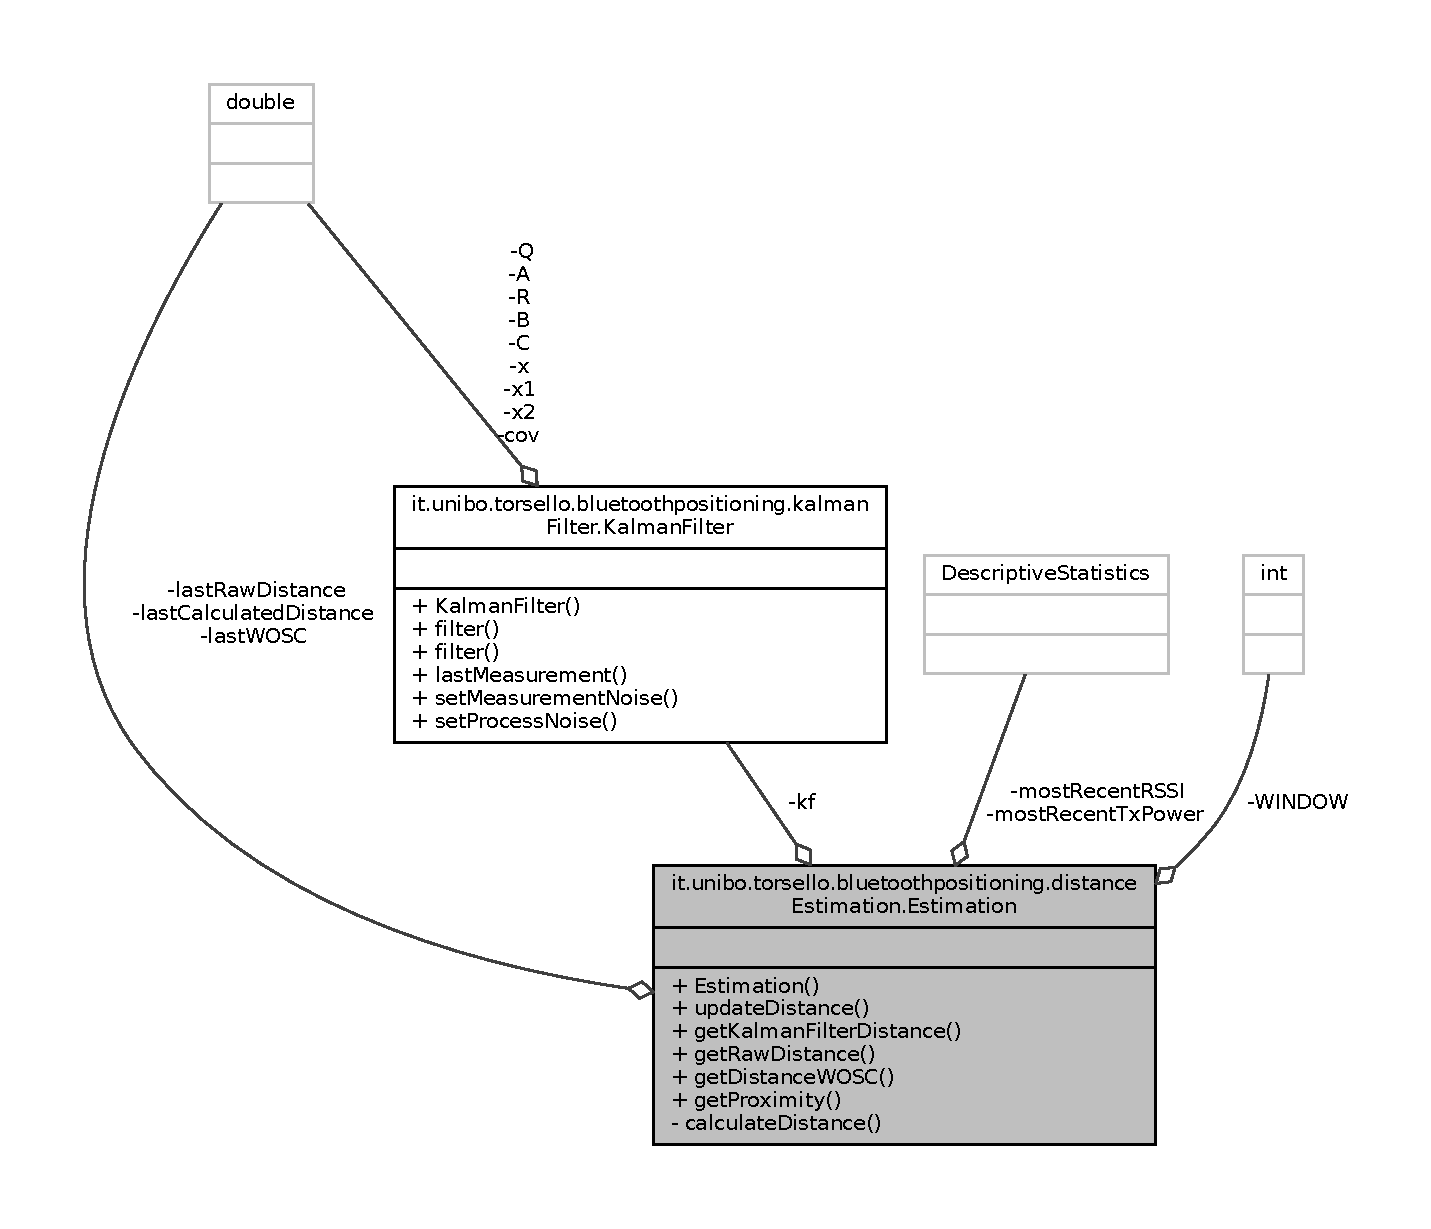
\includegraphics[width=350pt]{classit_1_1unibo_1_1torsello_1_1bluetoothpositioning_1_1distanceEstimation_1_1Estimation__coll__graph}
\end{center}
\end{figure}
\subsubsection*{Membri pubblici}
\begin{DoxyCompactItemize}
\item 
\hyperlink{classit_1_1unibo_1_1torsello_1_1bluetoothpositioning_1_1distanceEstimation_1_1Estimation_abd84ded1e26d40304606ce0572735106_abd84ded1e26d40304606ce0572735106}{Estimation} ()
\item 
void \hyperlink{classit_1_1unibo_1_1torsello_1_1bluetoothpositioning_1_1distanceEstimation_1_1Estimation_aaf86439861db7facf3f5338ec2fc6cde_aaf86439861db7facf3f5338ec2fc6cde}{update\+Distance} (Beacon b, double process\+Noise)
\item 
double \hyperlink{classit_1_1unibo_1_1torsello_1_1bluetoothpositioning_1_1distanceEstimation_1_1Estimation_a985e9b8b61c3d1e917a2e818b5f8b679_a985e9b8b61c3d1e917a2e818b5f8b679}{get\+Kalman\+Filter\+Distance} ()
\item 
double \hyperlink{classit_1_1unibo_1_1torsello_1_1bluetoothpositioning_1_1distanceEstimation_1_1Estimation_ad355b2e850a8d6013ef771eecd740e1b_ad355b2e850a8d6013ef771eecd740e1b}{get\+Raw\+Distance} ()
\item 
double \hyperlink{classit_1_1unibo_1_1torsello_1_1bluetoothpositioning_1_1distanceEstimation_1_1Estimation_a5c7bce21cd77c98a8d1e6df4c930397c_a5c7bce21cd77c98a8d1e6df4c930397c}{get\+Distance\+W\+O\+SC} ()
\item 
String \hyperlink{classit_1_1unibo_1_1torsello_1_1bluetoothpositioning_1_1distanceEstimation_1_1Estimation_a2edfb9f301730647277474c61b41dbd5_a2edfb9f301730647277474c61b41dbd5}{get\+Proximity} ()
\end{DoxyCompactItemize}
\subsubsection*{Membri privati}
\begin{DoxyCompactItemize}
\item 
double \hyperlink{classit_1_1unibo_1_1torsello_1_1bluetoothpositioning_1_1distanceEstimation_1_1Estimation_a6e33d4e0b776517a86c6aa87cd51b66b_a6e33d4e0b776517a86c6aa87cd51b66b}{calculate\+Distance} (double tx\+Power, double rssi)
\end{DoxyCompactItemize}
\subsubsection*{Attributi privati}
\begin{DoxyCompactItemize}
\item 
Descriptive\+Statistics \hyperlink{classit_1_1unibo_1_1torsello_1_1bluetoothpositioning_1_1distanceEstimation_1_1Estimation_a4edd1c580372b087a9d8fc167715088a_a4edd1c580372b087a9d8fc167715088a}{recent\+R\+S\+SI}
\item 
Descriptive\+Statistics \hyperlink{classit_1_1unibo_1_1torsello_1_1bluetoothpositioning_1_1distanceEstimation_1_1Estimation_a4258d96e807fa104223635ecb7ddc940_a4258d96e807fa104223635ecb7ddc940}{recent\+Tx\+Power}
\item 
\hyperlink{classit_1_1unibo_1_1torsello_1_1bluetoothpositioning_1_1kalmanFilter_1_1KFilter}{K\+Filter} \hyperlink{classit_1_1unibo_1_1torsello_1_1bluetoothpositioning_1_1distanceEstimation_1_1Estimation_a93af801219b710f3a048e7db1c7a8982_a93af801219b710f3a048e7db1c7a8982}{kf}
\item 
double \hyperlink{classit_1_1unibo_1_1torsello_1_1bluetoothpositioning_1_1distanceEstimation_1_1Estimation_a7a5514b25ac6495842a53e54319be10d_a7a5514b25ac6495842a53e54319be10d}{distance\+Estimated}
\item 
double \hyperlink{classit_1_1unibo_1_1torsello_1_1bluetoothpositioning_1_1distanceEstimation_1_1Estimation_a5afcd0b9b73a92b64669f060206f35db_a5afcd0b9b73a92b64669f060206f35db}{raw\+Distance\+Estimated}
\item 
double \hyperlink{classit_1_1unibo_1_1torsello_1_1bluetoothpositioning_1_1distanceEstimation_1_1Estimation_a53237b14bc1d27ae4f751b02d798b595_a53237b14bc1d27ae4f751b02d798b595}{W\+O\+SC}
\end{DoxyCompactItemize}


\subsubsection{Descrizione dettagliata}
Created by Federico Torsello. \href{mailto:federico.torsello@studio.unibo.it}{\tt federico.\+torsello@studio.\+unibo.\+it} 

\subsubsection{Documentazione dei costruttori e dei distruttori}
\hypertarget{classit_1_1unibo_1_1torsello_1_1bluetoothpositioning_1_1distanceEstimation_1_1Estimation_abd84ded1e26d40304606ce0572735106_abd84ded1e26d40304606ce0572735106}{}\label{classit_1_1unibo_1_1torsello_1_1bluetoothpositioning_1_1distanceEstimation_1_1Estimation_abd84ded1e26d40304606ce0572735106_abd84ded1e26d40304606ce0572735106} 
\index{it\+::unibo\+::torsello\+::bluetoothpositioning\+::distance\+Estimation\+::\+Estimation@{it\+::unibo\+::torsello\+::bluetoothpositioning\+::distance\+Estimation\+::\+Estimation}!Estimation@{Estimation}}
\index{Estimation@{Estimation}!it\+::unibo\+::torsello\+::bluetoothpositioning\+::distance\+Estimation\+::\+Estimation@{it\+::unibo\+::torsello\+::bluetoothpositioning\+::distance\+Estimation\+::\+Estimation}}
\paragraph{\texorpdfstring{Estimation()}{Estimation()}}
{\footnotesize\ttfamily it.\+unibo.\+torsello.\+bluetoothpositioning.\+distance\+Estimation.\+Estimation.\+Estimation (\begin{DoxyParamCaption}{ }\end{DoxyParamCaption})}


\begin{DoxyCode}
23                         \{
24 
25         \textcolor{comment}{// limit on the number of values that can be stored in the dataset}
26         \hyperlink{classit_1_1unibo_1_1torsello_1_1bluetoothpositioning_1_1distanceEstimation_1_1Estimation_a4edd1c580372b087a9d8fc167715088a_a4edd1c580372b087a9d8fc167715088a}{recentRSSI} = \textcolor{keyword}{new} DescriptiveStatistics();
27         \hyperlink{classit_1_1unibo_1_1torsello_1_1bluetoothpositioning_1_1distanceEstimation_1_1Estimation_a4edd1c580372b087a9d8fc167715088a_a4edd1c580372b087a9d8fc167715088a}{recentRSSI}.setWindowSize(KFilterConstants.WINDOW);
28         \hyperlink{classit_1_1unibo_1_1torsello_1_1bluetoothpositioning_1_1distanceEstimation_1_1Estimation_a4258d96e807fa104223635ecb7ddc940_a4258d96e807fa104223635ecb7ddc940}{recentTxPower} = \textcolor{keyword}{new} DescriptiveStatistics();
29         \hyperlink{classit_1_1unibo_1_1torsello_1_1bluetoothpositioning_1_1distanceEstimation_1_1Estimation_a4258d96e807fa104223635ecb7ddc940_a4258d96e807fa104223635ecb7ddc940}{recentTxPower}.setWindowSize(KFilterConstants.WINDOW);
30 
31         \hyperlink{classit_1_1unibo_1_1torsello_1_1bluetoothpositioning_1_1distanceEstimation_1_1Estimation_a7a5514b25ac6495842a53e54319be10d_a7a5514b25ac6495842a53e54319be10d}{distanceEstimated} = 0;
32         \hyperlink{classit_1_1unibo_1_1torsello_1_1bluetoothpositioning_1_1distanceEstimation_1_1Estimation_a5afcd0b9b73a92b64669f060206f35db_a5afcd0b9b73a92b64669f060206f35db}{rawDistanceEstimated} = 0;
33         \hyperlink{classit_1_1unibo_1_1torsello_1_1bluetoothpositioning_1_1distanceEstimation_1_1Estimation_a53237b14bc1d27ae4f751b02d798b595_a53237b14bc1d27ae4f751b02d798b595}{WOSC} = 0;
34 
35         \hyperlink{classit_1_1unibo_1_1torsello_1_1bluetoothpositioning_1_1distanceEstimation_1_1Estimation_a93af801219b710f3a048e7db1c7a8982_a93af801219b710f3a048e7db1c7a8982}{kf} = \textcolor{keyword}{new} KFilterBuilder()
36                 \textcolor{comment}{// filter for RSSI}
37                 .\hyperlink{classit_1_1unibo_1_1torsello_1_1bluetoothpositioning_1_1kalmanFilter_1_1KFilter_a8dd220ba0a0b0f20c368b13efeb1fe43_a8dd220ba0a0b0f20c368b13efeb1fe43}{R}(KFilterConstants.INITIAL\_PROCESS\_NOISE) \textcolor{comment}{// Initial process noise}
38                 .Q(KFilterConstants.INITIAL\_MEASUREMENT\_NOISE) \textcolor{comment}{// Initial measurement noise}
39                 .build();
40     \}
\end{DoxyCode}


\subsubsection{Documentazione delle funzioni membro}
\hypertarget{classit_1_1unibo_1_1torsello_1_1bluetoothpositioning_1_1distanceEstimation_1_1Estimation_a6e33d4e0b776517a86c6aa87cd51b66b_a6e33d4e0b776517a86c6aa87cd51b66b}{}\label{classit_1_1unibo_1_1torsello_1_1bluetoothpositioning_1_1distanceEstimation_1_1Estimation_a6e33d4e0b776517a86c6aa87cd51b66b_a6e33d4e0b776517a86c6aa87cd51b66b} 
\index{it\+::unibo\+::torsello\+::bluetoothpositioning\+::distance\+Estimation\+::\+Estimation@{it\+::unibo\+::torsello\+::bluetoothpositioning\+::distance\+Estimation\+::\+Estimation}!calculate\+Distance@{calculate\+Distance}}
\index{calculate\+Distance@{calculate\+Distance}!it\+::unibo\+::torsello\+::bluetoothpositioning\+::distance\+Estimation\+::\+Estimation@{it\+::unibo\+::torsello\+::bluetoothpositioning\+::distance\+Estimation\+::\+Estimation}}
\paragraph{\texorpdfstring{calculate\+Distance()}{calculateDistance()}}
{\footnotesize\ttfamily double it.\+unibo.\+torsello.\+bluetoothpositioning.\+distance\+Estimation.\+Estimation.\+calculate\+Distance (\begin{DoxyParamCaption}\item[{double}]{tx\+Power,  }\item[{double}]{rssi }\end{DoxyParamCaption})\hspace{0.3cm}{\ttfamily [private]}}


\begin{DoxyCode}
63                                                                   \{
64 
65         \textcolor{keywordflow}{if} (rssi == 0.0D) \{
66             \textcolor{keywordflow}{return} -1.0D; \textcolor{comment}{// if we cannot determine accuracy, return -1.}
67         \}
68 
69         \textcolor{keywordtype}{double} ratio = (rssi * 1.0D) / txPower;
70         \textcolor{keywordflow}{if} (ratio < 1.0D) \{
71             \textcolor{keywordflow}{return} Math.pow(ratio, 10.0D);
72         \}
73 
74 \textcolor{comment}{//        return (0.89976D * Math.pow(ratio, 7.7095D)) + 0.125D;}
75         \textcolor{keywordflow}{return} (0.89976D * Math.pow(ratio, 7.7095D)) + 0.111D;
76 
77     \textcolor{comment}{/*}
78 \textcolor{comment}{     * RSSI = TxPower - 10 * n * lg(d)}
79 \textcolor{comment}{     * n = 2 (in free space)}
80 \textcolor{comment}{     * d = 10 ^ ((TxPower - RSSI) / (10 * n))}
81 \textcolor{comment}{     */}
82         \textcolor{comment}{// return Math.pow(10D, (txPower - rssi) / (10 * 2));}
83     \}
\end{DoxyCode}
\hypertarget{classit_1_1unibo_1_1torsello_1_1bluetoothpositioning_1_1distanceEstimation_1_1Estimation_a5c7bce21cd77c98a8d1e6df4c930397c_a5c7bce21cd77c98a8d1e6df4c930397c}{}\label{classit_1_1unibo_1_1torsello_1_1bluetoothpositioning_1_1distanceEstimation_1_1Estimation_a5c7bce21cd77c98a8d1e6df4c930397c_a5c7bce21cd77c98a8d1e6df4c930397c} 
\index{it\+::unibo\+::torsello\+::bluetoothpositioning\+::distance\+Estimation\+::\+Estimation@{it\+::unibo\+::torsello\+::bluetoothpositioning\+::distance\+Estimation\+::\+Estimation}!get\+Distance\+W\+O\+SC@{get\+Distance\+W\+O\+SC}}
\index{get\+Distance\+W\+O\+SC@{get\+Distance\+W\+O\+SC}!it\+::unibo\+::torsello\+::bluetoothpositioning\+::distance\+Estimation\+::\+Estimation@{it\+::unibo\+::torsello\+::bluetoothpositioning\+::distance\+Estimation\+::\+Estimation}}
\paragraph{\texorpdfstring{get\+Distance\+W\+O\+S\+C()}{getDistanceWOSC()}}
{\footnotesize\ttfamily double it.\+unibo.\+torsello.\+bluetoothpositioning.\+distance\+Estimation.\+Estimation.\+get\+Distance\+W\+O\+SC (\begin{DoxyParamCaption}{ }\end{DoxyParamCaption})}


\begin{DoxyCode}
93                                     \{
94         \textcolor{keywordflow}{return} \hyperlink{classit_1_1unibo_1_1torsello_1_1bluetoothpositioning_1_1distanceEstimation_1_1Estimation_a53237b14bc1d27ae4f751b02d798b595_a53237b14bc1d27ae4f751b02d798b595}{WOSC};
95     \}
\end{DoxyCode}
\hypertarget{classit_1_1unibo_1_1torsello_1_1bluetoothpositioning_1_1distanceEstimation_1_1Estimation_a985e9b8b61c3d1e917a2e818b5f8b679_a985e9b8b61c3d1e917a2e818b5f8b679}{}\label{classit_1_1unibo_1_1torsello_1_1bluetoothpositioning_1_1distanceEstimation_1_1Estimation_a985e9b8b61c3d1e917a2e818b5f8b679_a985e9b8b61c3d1e917a2e818b5f8b679} 
\index{it\+::unibo\+::torsello\+::bluetoothpositioning\+::distance\+Estimation\+::\+Estimation@{it\+::unibo\+::torsello\+::bluetoothpositioning\+::distance\+Estimation\+::\+Estimation}!get\+Kalman\+Filter\+Distance@{get\+Kalman\+Filter\+Distance}}
\index{get\+Kalman\+Filter\+Distance@{get\+Kalman\+Filter\+Distance}!it\+::unibo\+::torsello\+::bluetoothpositioning\+::distance\+Estimation\+::\+Estimation@{it\+::unibo\+::torsello\+::bluetoothpositioning\+::distance\+Estimation\+::\+Estimation}}
\paragraph{\texorpdfstring{get\+Kalman\+Filter\+Distance()}{getKalmanFilterDistance()}}
{\footnotesize\ttfamily double it.\+unibo.\+torsello.\+bluetoothpositioning.\+distance\+Estimation.\+Estimation.\+get\+Kalman\+Filter\+Distance (\begin{DoxyParamCaption}{ }\end{DoxyParamCaption})}


\begin{DoxyCode}
85                                             \{
86         \textcolor{keywordflow}{return} \hyperlink{classit_1_1unibo_1_1torsello_1_1bluetoothpositioning_1_1distanceEstimation_1_1Estimation_a7a5514b25ac6495842a53e54319be10d_a7a5514b25ac6495842a53e54319be10d}{distanceEstimated};
87     \}
\end{DoxyCode}
\hypertarget{classit_1_1unibo_1_1torsello_1_1bluetoothpositioning_1_1distanceEstimation_1_1Estimation_a2edfb9f301730647277474c61b41dbd5_a2edfb9f301730647277474c61b41dbd5}{}\label{classit_1_1unibo_1_1torsello_1_1bluetoothpositioning_1_1distanceEstimation_1_1Estimation_a2edfb9f301730647277474c61b41dbd5_a2edfb9f301730647277474c61b41dbd5} 
\index{it\+::unibo\+::torsello\+::bluetoothpositioning\+::distance\+Estimation\+::\+Estimation@{it\+::unibo\+::torsello\+::bluetoothpositioning\+::distance\+Estimation\+::\+Estimation}!get\+Proximity@{get\+Proximity}}
\index{get\+Proximity@{get\+Proximity}!it\+::unibo\+::torsello\+::bluetoothpositioning\+::distance\+Estimation\+::\+Estimation@{it\+::unibo\+::torsello\+::bluetoothpositioning\+::distance\+Estimation\+::\+Estimation}}
\paragraph{\texorpdfstring{get\+Proximity()}{getProximity()}}
{\footnotesize\ttfamily String it.\+unibo.\+torsello.\+bluetoothpositioning.\+distance\+Estimation.\+Estimation.\+get\+Proximity (\begin{DoxyParamCaption}{ }\end{DoxyParamCaption})}


\begin{DoxyCode}
97                                  \{
98         \textcolor{keywordtype}{double} proximity = \hyperlink{classit_1_1unibo_1_1torsello_1_1bluetoothpositioning_1_1distanceEstimation_1_1Estimation_a7a5514b25ac6495842a53e54319be10d_a7a5514b25ac6495842a53e54319be10d}{distanceEstimated};
99         String accuracy;
100 
101         \textcolor{keywordflow}{if} (proximity <= 0) \{
102             accuracy = \textcolor{stringliteral}{"unknown"};
103         \} \textcolor{keywordflow}{else} \textcolor{keywordflow}{if} (proximity <= 0.5) \{
104             accuracy = \textcolor{stringliteral}{"immediate"};
105         \} \textcolor{keywordflow}{else} \textcolor{keywordflow}{if} (proximity <= 4.0) \{
106             accuracy = \textcolor{stringliteral}{"near"};
107         \} \textcolor{keywordflow}{else} \{
108             accuracy = \textcolor{stringliteral}{"far"};
109         \}
110         \textcolor{keywordflow}{return} accuracy;
111     \}
\end{DoxyCode}
\hypertarget{classit_1_1unibo_1_1torsello_1_1bluetoothpositioning_1_1distanceEstimation_1_1Estimation_ad355b2e850a8d6013ef771eecd740e1b_ad355b2e850a8d6013ef771eecd740e1b}{}\label{classit_1_1unibo_1_1torsello_1_1bluetoothpositioning_1_1distanceEstimation_1_1Estimation_ad355b2e850a8d6013ef771eecd740e1b_ad355b2e850a8d6013ef771eecd740e1b} 
\index{it\+::unibo\+::torsello\+::bluetoothpositioning\+::distance\+Estimation\+::\+Estimation@{it\+::unibo\+::torsello\+::bluetoothpositioning\+::distance\+Estimation\+::\+Estimation}!get\+Raw\+Distance@{get\+Raw\+Distance}}
\index{get\+Raw\+Distance@{get\+Raw\+Distance}!it\+::unibo\+::torsello\+::bluetoothpositioning\+::distance\+Estimation\+::\+Estimation@{it\+::unibo\+::torsello\+::bluetoothpositioning\+::distance\+Estimation\+::\+Estimation}}
\paragraph{\texorpdfstring{get\+Raw\+Distance()}{getRawDistance()}}
{\footnotesize\ttfamily double it.\+unibo.\+torsello.\+bluetoothpositioning.\+distance\+Estimation.\+Estimation.\+get\+Raw\+Distance (\begin{DoxyParamCaption}{ }\end{DoxyParamCaption})}


\begin{DoxyCode}
89                                    \{
90         \textcolor{keywordflow}{return} \hyperlink{classit_1_1unibo_1_1torsello_1_1bluetoothpositioning_1_1distanceEstimation_1_1Estimation_a5afcd0b9b73a92b64669f060206f35db_a5afcd0b9b73a92b64669f060206f35db}{rawDistanceEstimated};
91     \}
\end{DoxyCode}
\hypertarget{classit_1_1unibo_1_1torsello_1_1bluetoothpositioning_1_1distanceEstimation_1_1Estimation_aaf86439861db7facf3f5338ec2fc6cde_aaf86439861db7facf3f5338ec2fc6cde}{}\label{classit_1_1unibo_1_1torsello_1_1bluetoothpositioning_1_1distanceEstimation_1_1Estimation_aaf86439861db7facf3f5338ec2fc6cde_aaf86439861db7facf3f5338ec2fc6cde} 
\index{it\+::unibo\+::torsello\+::bluetoothpositioning\+::distance\+Estimation\+::\+Estimation@{it\+::unibo\+::torsello\+::bluetoothpositioning\+::distance\+Estimation\+::\+Estimation}!update\+Distance@{update\+Distance}}
\index{update\+Distance@{update\+Distance}!it\+::unibo\+::torsello\+::bluetoothpositioning\+::distance\+Estimation\+::\+Estimation@{it\+::unibo\+::torsello\+::bluetoothpositioning\+::distance\+Estimation\+::\+Estimation}}
\paragraph{\texorpdfstring{update\+Distance()}{updateDistance()}}
{\footnotesize\ttfamily void it.\+unibo.\+torsello.\+bluetoothpositioning.\+distance\+Estimation.\+Estimation.\+update\+Distance (\begin{DoxyParamCaption}\item[{Beacon}]{b,  }\item[{double}]{process\+Noise }\end{DoxyParamCaption})}


\begin{DoxyCode}
42                                                               \{
43 
44         \hyperlink{classit_1_1unibo_1_1torsello_1_1bluetoothpositioning_1_1distanceEstimation_1_1Estimation_a4edd1c580372b087a9d8fc167715088a_a4edd1c580372b087a9d8fc167715088a}{recentRSSI}.addValue(b.getRssi());
45         \hyperlink{classit_1_1unibo_1_1torsello_1_1bluetoothpositioning_1_1distanceEstimation_1_1Estimation_a4258d96e807fa104223635ecb7ddc940_a4258d96e807fa104223635ecb7ddc940}{recentTxPower}.addValue(b.getTxPower());
46 
47         \textcolor{comment}{// Update measurement noise continually}
48         \textcolor{keywordtype}{double} mNoise = Math.sqrt((100 * 9 / Math.log(10)) *
49                 Math.log(1 + Math.pow(\hyperlink{classit_1_1unibo_1_1torsello_1_1bluetoothpositioning_1_1distanceEstimation_1_1Estimation_a4edd1c580372b087a9d8fc167715088a_a4edd1c580372b087a9d8fc167715088a}{recentRSSI}.getMean() / 
      \hyperlink{classit_1_1unibo_1_1torsello_1_1bluetoothpositioning_1_1distanceEstimation_1_1Estimation_a4edd1c580372b087a9d8fc167715088a_a4edd1c580372b087a9d8fc167715088a}{recentRSSI}.getStandardDeviation(), 2)));
50 
51         \textcolor{keywordflow}{if} (!Double.isInfinite(mNoise) && !Double.isNaN(mNoise)) \{
52             \hyperlink{classit_1_1unibo_1_1torsello_1_1bluetoothpositioning_1_1distanceEstimation_1_1Estimation_a93af801219b710f3a048e7db1c7a8982_a93af801219b710f3a048e7db1c7a8982}{kf}.\hyperlink{classit_1_1unibo_1_1torsello_1_1bluetoothpositioning_1_1kalmanFilter_1_1KFilter_a0ed62a630ff52aacdcd8832b9416f406_a0ed62a630ff52aacdcd8832b9416f406}{setMeasurementNoise}(mNoise);
53         \}
54 
55         \hyperlink{classit_1_1unibo_1_1torsello_1_1bluetoothpositioning_1_1distanceEstimation_1_1Estimation_a93af801219b710f3a048e7db1c7a8982_a93af801219b710f3a048e7db1c7a8982}{kf}.\hyperlink{classit_1_1unibo_1_1torsello_1_1bluetoothpositioning_1_1kalmanFilter_1_1KFilter_a7651339cfddb4cdaa1e47906b27745fc_a7651339cfddb4cdaa1e47906b27745fc}{setProcessNoise}(processNoise);
56         \textcolor{keywordtype}{double} lastFilteredReading = \hyperlink{classit_1_1unibo_1_1torsello_1_1bluetoothpositioning_1_1distanceEstimation_1_1Estimation_a93af801219b710f3a048e7db1c7a8982_a93af801219b710f3a048e7db1c7a8982}{kf}.\hyperlink{classit_1_1unibo_1_1torsello_1_1bluetoothpositioning_1_1kalmanFilter_1_1KFilter_a6904818e94d959f8e25a8699d6885c21_a6904818e94d959f8e25a8699d6885c21}{filter}(\hyperlink{classit_1_1unibo_1_1torsello_1_1bluetoothpositioning_1_1distanceEstimation_1_1Estimation_a4edd1c580372b087a9d8fc167715088a_a4edd1c580372b087a9d8fc167715088a}{recentRSSI}.getPercentile(50));
57         \hyperlink{classit_1_1unibo_1_1torsello_1_1bluetoothpositioning_1_1distanceEstimation_1_1Estimation_a7a5514b25ac6495842a53e54319be10d_a7a5514b25ac6495842a53e54319be10d}{distanceEstimated} = \hyperlink{classit_1_1unibo_1_1torsello_1_1bluetoothpositioning_1_1distanceEstimation_1_1Estimation_a6e33d4e0b776517a86c6aa87cd51b66b_a6e33d4e0b776517a86c6aa87cd51b66b}{calculateDistance}(
      \hyperlink{classit_1_1unibo_1_1torsello_1_1bluetoothpositioning_1_1distanceEstimation_1_1Estimation_a4258d96e807fa104223635ecb7ddc940_a4258d96e807fa104223635ecb7ddc940}{recentTxPower}.getPercentile(50), lastFilteredReading);
58         \hyperlink{classit_1_1unibo_1_1torsello_1_1bluetoothpositioning_1_1distanceEstimation_1_1Estimation_a5afcd0b9b73a92b64669f060206f35db_a5afcd0b9b73a92b64669f060206f35db}{rawDistanceEstimated} = \hyperlink{classit_1_1unibo_1_1torsello_1_1bluetoothpositioning_1_1distanceEstimation_1_1Estimation_a6e33d4e0b776517a86c6aa87cd51b66b_a6e33d4e0b776517a86c6aa87cd51b66b}{calculateDistance}(b.getTxPower(), b.
      getRssi());
59         \hyperlink{classit_1_1unibo_1_1torsello_1_1bluetoothpositioning_1_1distanceEstimation_1_1Estimation_a53237b14bc1d27ae4f751b02d798b595_a53237b14bc1d27ae4f751b02d798b595}{WOSC} = \hyperlink{classit_1_1unibo_1_1torsello_1_1bluetoothpositioning_1_1distanceEstimation_1_1Estimation_a6e33d4e0b776517a86c6aa87cd51b66b_a6e33d4e0b776517a86c6aa87cd51b66b}{calculateDistance}(b.getTxPower(), lastFilteredReading);
60     \}
\end{DoxyCode}


\subsubsection{Documentazione dei membri dato}
\hypertarget{classit_1_1unibo_1_1torsello_1_1bluetoothpositioning_1_1distanceEstimation_1_1Estimation_a7a5514b25ac6495842a53e54319be10d_a7a5514b25ac6495842a53e54319be10d}{}\label{classit_1_1unibo_1_1torsello_1_1bluetoothpositioning_1_1distanceEstimation_1_1Estimation_a7a5514b25ac6495842a53e54319be10d_a7a5514b25ac6495842a53e54319be10d} 
\index{it\+::unibo\+::torsello\+::bluetoothpositioning\+::distance\+Estimation\+::\+Estimation@{it\+::unibo\+::torsello\+::bluetoothpositioning\+::distance\+Estimation\+::\+Estimation}!distance\+Estimated@{distance\+Estimated}}
\index{distance\+Estimated@{distance\+Estimated}!it\+::unibo\+::torsello\+::bluetoothpositioning\+::distance\+Estimation\+::\+Estimation@{it\+::unibo\+::torsello\+::bluetoothpositioning\+::distance\+Estimation\+::\+Estimation}}
\paragraph{\texorpdfstring{distance\+Estimated}{distanceEstimated}}
{\footnotesize\ttfamily double it.\+unibo.\+torsello.\+bluetoothpositioning.\+distance\+Estimation.\+Estimation.\+distance\+Estimated\hspace{0.3cm}{\ttfamily [private]}}

\hypertarget{classit_1_1unibo_1_1torsello_1_1bluetoothpositioning_1_1distanceEstimation_1_1Estimation_a93af801219b710f3a048e7db1c7a8982_a93af801219b710f3a048e7db1c7a8982}{}\label{classit_1_1unibo_1_1torsello_1_1bluetoothpositioning_1_1distanceEstimation_1_1Estimation_a93af801219b710f3a048e7db1c7a8982_a93af801219b710f3a048e7db1c7a8982} 
\index{it\+::unibo\+::torsello\+::bluetoothpositioning\+::distance\+Estimation\+::\+Estimation@{it\+::unibo\+::torsello\+::bluetoothpositioning\+::distance\+Estimation\+::\+Estimation}!kf@{kf}}
\index{kf@{kf}!it\+::unibo\+::torsello\+::bluetoothpositioning\+::distance\+Estimation\+::\+Estimation@{it\+::unibo\+::torsello\+::bluetoothpositioning\+::distance\+Estimation\+::\+Estimation}}
\paragraph{\texorpdfstring{kf}{kf}}
{\footnotesize\ttfamily \hyperlink{classit_1_1unibo_1_1torsello_1_1bluetoothpositioning_1_1kalmanFilter_1_1KFilter}{K\+Filter} it.\+unibo.\+torsello.\+bluetoothpositioning.\+distance\+Estimation.\+Estimation.\+kf\hspace{0.3cm}{\ttfamily [private]}}

\hypertarget{classit_1_1unibo_1_1torsello_1_1bluetoothpositioning_1_1distanceEstimation_1_1Estimation_a5afcd0b9b73a92b64669f060206f35db_a5afcd0b9b73a92b64669f060206f35db}{}\label{classit_1_1unibo_1_1torsello_1_1bluetoothpositioning_1_1distanceEstimation_1_1Estimation_a5afcd0b9b73a92b64669f060206f35db_a5afcd0b9b73a92b64669f060206f35db} 
\index{it\+::unibo\+::torsello\+::bluetoothpositioning\+::distance\+Estimation\+::\+Estimation@{it\+::unibo\+::torsello\+::bluetoothpositioning\+::distance\+Estimation\+::\+Estimation}!raw\+Distance\+Estimated@{raw\+Distance\+Estimated}}
\index{raw\+Distance\+Estimated@{raw\+Distance\+Estimated}!it\+::unibo\+::torsello\+::bluetoothpositioning\+::distance\+Estimation\+::\+Estimation@{it\+::unibo\+::torsello\+::bluetoothpositioning\+::distance\+Estimation\+::\+Estimation}}
\paragraph{\texorpdfstring{raw\+Distance\+Estimated}{rawDistanceEstimated}}
{\footnotesize\ttfamily double it.\+unibo.\+torsello.\+bluetoothpositioning.\+distance\+Estimation.\+Estimation.\+raw\+Distance\+Estimated\hspace{0.3cm}{\ttfamily [private]}}

\hypertarget{classit_1_1unibo_1_1torsello_1_1bluetoothpositioning_1_1distanceEstimation_1_1Estimation_a4edd1c580372b087a9d8fc167715088a_a4edd1c580372b087a9d8fc167715088a}{}\label{classit_1_1unibo_1_1torsello_1_1bluetoothpositioning_1_1distanceEstimation_1_1Estimation_a4edd1c580372b087a9d8fc167715088a_a4edd1c580372b087a9d8fc167715088a} 
\index{it\+::unibo\+::torsello\+::bluetoothpositioning\+::distance\+Estimation\+::\+Estimation@{it\+::unibo\+::torsello\+::bluetoothpositioning\+::distance\+Estimation\+::\+Estimation}!recent\+R\+S\+SI@{recent\+R\+S\+SI}}
\index{recent\+R\+S\+SI@{recent\+R\+S\+SI}!it\+::unibo\+::torsello\+::bluetoothpositioning\+::distance\+Estimation\+::\+Estimation@{it\+::unibo\+::torsello\+::bluetoothpositioning\+::distance\+Estimation\+::\+Estimation}}
\paragraph{\texorpdfstring{recent\+R\+S\+SI}{recentRSSI}}
{\footnotesize\ttfamily Descriptive\+Statistics it.\+unibo.\+torsello.\+bluetoothpositioning.\+distance\+Estimation.\+Estimation.\+recent\+R\+S\+SI\hspace{0.3cm}{\ttfamily [private]}}

\hypertarget{classit_1_1unibo_1_1torsello_1_1bluetoothpositioning_1_1distanceEstimation_1_1Estimation_a4258d96e807fa104223635ecb7ddc940_a4258d96e807fa104223635ecb7ddc940}{}\label{classit_1_1unibo_1_1torsello_1_1bluetoothpositioning_1_1distanceEstimation_1_1Estimation_a4258d96e807fa104223635ecb7ddc940_a4258d96e807fa104223635ecb7ddc940} 
\index{it\+::unibo\+::torsello\+::bluetoothpositioning\+::distance\+Estimation\+::\+Estimation@{it\+::unibo\+::torsello\+::bluetoothpositioning\+::distance\+Estimation\+::\+Estimation}!recent\+Tx\+Power@{recent\+Tx\+Power}}
\index{recent\+Tx\+Power@{recent\+Tx\+Power}!it\+::unibo\+::torsello\+::bluetoothpositioning\+::distance\+Estimation\+::\+Estimation@{it\+::unibo\+::torsello\+::bluetoothpositioning\+::distance\+Estimation\+::\+Estimation}}
\paragraph{\texorpdfstring{recent\+Tx\+Power}{recentTxPower}}
{\footnotesize\ttfamily Descriptive\+Statistics it.\+unibo.\+torsello.\+bluetoothpositioning.\+distance\+Estimation.\+Estimation.\+recent\+Tx\+Power\hspace{0.3cm}{\ttfamily [private]}}

\hypertarget{classit_1_1unibo_1_1torsello_1_1bluetoothpositioning_1_1distanceEstimation_1_1Estimation_a53237b14bc1d27ae4f751b02d798b595_a53237b14bc1d27ae4f751b02d798b595}{}\label{classit_1_1unibo_1_1torsello_1_1bluetoothpositioning_1_1distanceEstimation_1_1Estimation_a53237b14bc1d27ae4f751b02d798b595_a53237b14bc1d27ae4f751b02d798b595} 
\index{it\+::unibo\+::torsello\+::bluetoothpositioning\+::distance\+Estimation\+::\+Estimation@{it\+::unibo\+::torsello\+::bluetoothpositioning\+::distance\+Estimation\+::\+Estimation}!W\+O\+SC@{W\+O\+SC}}
\index{W\+O\+SC@{W\+O\+SC}!it\+::unibo\+::torsello\+::bluetoothpositioning\+::distance\+Estimation\+::\+Estimation@{it\+::unibo\+::torsello\+::bluetoothpositioning\+::distance\+Estimation\+::\+Estimation}}
\paragraph{\texorpdfstring{W\+O\+SC}{WOSC}}
{\footnotesize\ttfamily double it.\+unibo.\+torsello.\+bluetoothpositioning.\+distance\+Estimation.\+Estimation.\+W\+O\+SC\hspace{0.3cm}{\ttfamily [private]}}



La documentazione per questa classe è stata generata a partire dal seguente file\+:\begin{DoxyCompactItemize}
\item 
\hyperlink{Estimation_8java}{Estimation.\+java}\end{DoxyCompactItemize}

\hypertarget{classit_1_1unibo_1_1torsello_1_1bluetoothpositioning_1_1extra_1_1FABBehavior}{}\subsection{Riferimenti per la classe it.\+unibo.\+torsello.\+bluetoothpositioning.\+extra.\+F\+A\+B\+Behavior}
\label{classit_1_1unibo_1_1torsello_1_1bluetoothpositioning_1_1extra_1_1FABBehavior}\index{it.\+unibo.\+torsello.\+bluetoothpositioning.\+extra.\+F\+A\+B\+Behavior@{it.\+unibo.\+torsello.\+bluetoothpositioning.\+extra.\+F\+A\+B\+Behavior}}


Diagramma delle classi per it.\+unibo.\+torsello.\+bluetoothpositioning.\+extra.\+F\+A\+B\+Behavior
\nopagebreak
\begin{figure}[H]
\begin{center}
\leavevmode
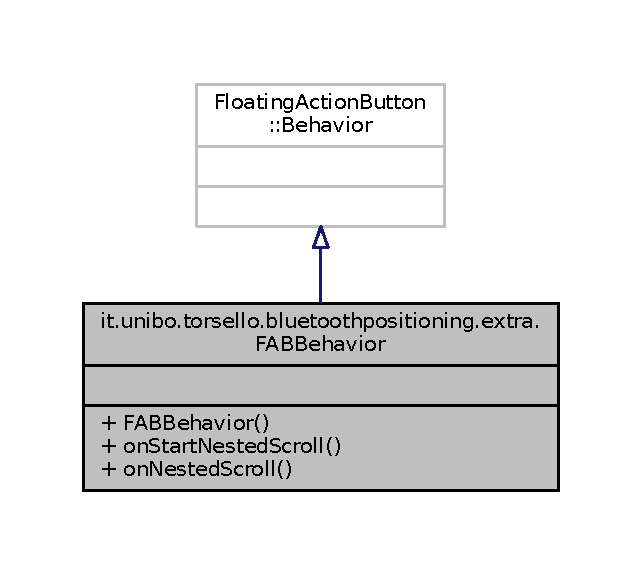
\includegraphics[width=308pt]{classit_1_1unibo_1_1torsello_1_1bluetoothpositioning_1_1extra_1_1FABBehavior__inherit__graph}
\end{center}
\end{figure}


Diagramma di collaborazione per it.\+unibo.\+torsello.\+bluetoothpositioning.\+extra.\+F\+A\+B\+Behavior\+:
\nopagebreak
\begin{figure}[H]
\begin{center}
\leavevmode
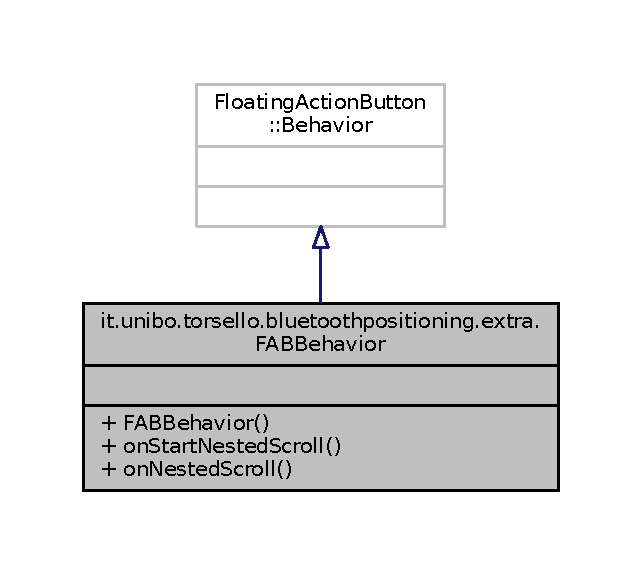
\includegraphics[width=308pt]{classit_1_1unibo_1_1torsello_1_1bluetoothpositioning_1_1extra_1_1FABBehavior__coll__graph}
\end{center}
\end{figure}
\subsubsection*{Membri pubblici}
\begin{DoxyCompactItemize}
\item 
\hyperlink{classit_1_1unibo_1_1torsello_1_1bluetoothpositioning_1_1extra_1_1FABBehavior_ae703e3a3d6d647561f7b41a0eb94a9f0_ae703e3a3d6d647561f7b41a0eb94a9f0}{F\+A\+B\+Behavior} (Context context, Attribute\+Set attrs)
\item 
boolean \hyperlink{classit_1_1unibo_1_1torsello_1_1bluetoothpositioning_1_1extra_1_1FABBehavior_a5c6501a08ec79dd6bd92106b72c14979_a5c6501a08ec79dd6bd92106b72c14979}{on\+Start\+Nested\+Scroll} (Coordinator\+Layout coordinator\+Layout, final Floating\+Action\+Button child, View direct\+Target\+Child, View target, int nested\+Scroll\+Axes)
\item 
void \hyperlink{classit_1_1unibo_1_1torsello_1_1bluetoothpositioning_1_1extra_1_1FABBehavior_ab4208eb2a50a8e79e0a80089f398a5b9_ab4208eb2a50a8e79e0a80089f398a5b9}{on\+Nested\+Scroll} (Coordinator\+Layout coordinator\+Layout, final Floating\+Action\+Button child, View target, int dx\+Consumed, int dy\+Consumed, int dx\+Unconsumed, int dy\+Unconsumed)
\end{DoxyCompactItemize}


\subsubsection{Descrizione dettagliata}
Created by Federico Torsello. \href{mailto:federico.torsello@studio.unibo.it}{\tt federico.\+torsello@studio.\+unibo.\+it} 

\subsubsection{Documentazione dei costruttori e dei distruttori}
\hypertarget{classit_1_1unibo_1_1torsello_1_1bluetoothpositioning_1_1extra_1_1FABBehavior_ae703e3a3d6d647561f7b41a0eb94a9f0_ae703e3a3d6d647561f7b41a0eb94a9f0}{}\label{classit_1_1unibo_1_1torsello_1_1bluetoothpositioning_1_1extra_1_1FABBehavior_ae703e3a3d6d647561f7b41a0eb94a9f0_ae703e3a3d6d647561f7b41a0eb94a9f0} 
\index{it\+::unibo\+::torsello\+::bluetoothpositioning\+::extra\+::\+F\+A\+B\+Behavior@{it\+::unibo\+::torsello\+::bluetoothpositioning\+::extra\+::\+F\+A\+B\+Behavior}!F\+A\+B\+Behavior@{F\+A\+B\+Behavior}}
\index{F\+A\+B\+Behavior@{F\+A\+B\+Behavior}!it\+::unibo\+::torsello\+::bluetoothpositioning\+::extra\+::\+F\+A\+B\+Behavior@{it\+::unibo\+::torsello\+::bluetoothpositioning\+::extra\+::\+F\+A\+B\+Behavior}}
\paragraph{\texorpdfstring{F\+A\+B\+Behavior()}{FABBehavior()}}
{\footnotesize\ttfamily it.\+unibo.\+torsello.\+bluetoothpositioning.\+extra.\+F\+A\+B\+Behavior.\+F\+A\+B\+Behavior (\begin{DoxyParamCaption}\item[{Context}]{context,  }\item[{Attribute\+Set}]{attrs }\end{DoxyParamCaption})}


\begin{DoxyCode}
18                                                             \{
19         super();
20     \}
\end{DoxyCode}


\subsubsection{Documentazione delle funzioni membro}
\hypertarget{classit_1_1unibo_1_1torsello_1_1bluetoothpositioning_1_1extra_1_1FABBehavior_ab4208eb2a50a8e79e0a80089f398a5b9_ab4208eb2a50a8e79e0a80089f398a5b9}{}\label{classit_1_1unibo_1_1torsello_1_1bluetoothpositioning_1_1extra_1_1FABBehavior_ab4208eb2a50a8e79e0a80089f398a5b9_ab4208eb2a50a8e79e0a80089f398a5b9} 
\index{it\+::unibo\+::torsello\+::bluetoothpositioning\+::extra\+::\+F\+A\+B\+Behavior@{it\+::unibo\+::torsello\+::bluetoothpositioning\+::extra\+::\+F\+A\+B\+Behavior}!on\+Nested\+Scroll@{on\+Nested\+Scroll}}
\index{on\+Nested\+Scroll@{on\+Nested\+Scroll}!it\+::unibo\+::torsello\+::bluetoothpositioning\+::extra\+::\+F\+A\+B\+Behavior@{it\+::unibo\+::torsello\+::bluetoothpositioning\+::extra\+::\+F\+A\+B\+Behavior}}
\paragraph{\texorpdfstring{on\+Nested\+Scroll()}{onNestedScroll()}}
{\footnotesize\ttfamily void it.\+unibo.\+torsello.\+bluetoothpositioning.\+extra.\+F\+A\+B\+Behavior.\+on\+Nested\+Scroll (\begin{DoxyParamCaption}\item[{Coordinator\+Layout}]{coordinator\+Layout,  }\item[{final Floating\+Action\+Button}]{child,  }\item[{View}]{target,  }\item[{int}]{dx\+Consumed,  }\item[{int}]{dy\+Consumed,  }\item[{int}]{dx\+Unconsumed,  }\item[{int}]{dy\+Unconsumed }\end{DoxyParamCaption})}


\begin{DoxyCode}
34                                                                                                            
           \{
35         super.onNestedScroll(coordinatorLayout, child, target, dxConsumed, dyConsumed, dxUnconsumed,
36                 dyUnconsumed);
37 
38         \textcolor{keywordflow}{if} ((dyConsumed > 0 || dyUnconsumed == 0) && child.getVisibility() == View.VISIBLE) \{
39             child.hide();
40             \textcolor{keyword}{new} Handler().postDelayed(\textcolor{keyword}{new} Runnable() \{
41                 @Override
42                 \textcolor{keyword}{public} \textcolor{keywordtype}{void} run() \{
43                     child.show();
44                 \}
45             \}, 1000);
46         \}
47     \}
\end{DoxyCode}
\hypertarget{classit_1_1unibo_1_1torsello_1_1bluetoothpositioning_1_1extra_1_1FABBehavior_a5c6501a08ec79dd6bd92106b72c14979_a5c6501a08ec79dd6bd92106b72c14979}{}\label{classit_1_1unibo_1_1torsello_1_1bluetoothpositioning_1_1extra_1_1FABBehavior_a5c6501a08ec79dd6bd92106b72c14979_a5c6501a08ec79dd6bd92106b72c14979} 
\index{it\+::unibo\+::torsello\+::bluetoothpositioning\+::extra\+::\+F\+A\+B\+Behavior@{it\+::unibo\+::torsello\+::bluetoothpositioning\+::extra\+::\+F\+A\+B\+Behavior}!on\+Start\+Nested\+Scroll@{on\+Start\+Nested\+Scroll}}
\index{on\+Start\+Nested\+Scroll@{on\+Start\+Nested\+Scroll}!it\+::unibo\+::torsello\+::bluetoothpositioning\+::extra\+::\+F\+A\+B\+Behavior@{it\+::unibo\+::torsello\+::bluetoothpositioning\+::extra\+::\+F\+A\+B\+Behavior}}
\paragraph{\texorpdfstring{on\+Start\+Nested\+Scroll()}{onStartNestedScroll()}}
{\footnotesize\ttfamily boolean it.\+unibo.\+torsello.\+bluetoothpositioning.\+extra.\+F\+A\+B\+Behavior.\+on\+Start\+Nested\+Scroll (\begin{DoxyParamCaption}\item[{Coordinator\+Layout}]{coordinator\+Layout,  }\item[{final Floating\+Action\+Button}]{child,  }\item[{View}]{direct\+Target\+Child,  }\item[{View}]{target,  }\item[{int}]{nested\+Scroll\+Axes }\end{DoxyParamCaption})}


\begin{DoxyCode}
24                                                                                                   \{
25 
26 \textcolor{comment}{//        return nestedScrollAxes == ViewCompat.SCROLL\_AXIS\_VERTICAL ||}
27 \textcolor{comment}{//                super.onStartNestedScroll(coordinatorLayout, child, directTargetChild, target,}
28 \textcolor{comment}{//                        nestedScrollAxes);}
29         \textcolor{keywordflow}{return} \textcolor{keyword}{true};
30     \}
\end{DoxyCode}


La documentazione per questa classe è stata generata a partire dal seguente file\+:\begin{DoxyCompactItemize}
\item 
\hyperlink{FABBehavior_8java}{F\+A\+B\+Behavior.\+java}\end{DoxyCompactItemize}

\hypertarget{classit_1_1unibo_1_1torsello_1_1bluetoothpositioning_1_1kalmanFilter_1_1KalmanFilter}{}\subsection{Riferimenti per la classe it.\+unibo.\+torsello.\+bluetoothpositioning.\+kalman\+Filter.\+Kalman\+Filter}
\label{classit_1_1unibo_1_1torsello_1_1bluetoothpositioning_1_1kalmanFilter_1_1KalmanFilter}\index{it.\+unibo.\+torsello.\+bluetoothpositioning.\+kalman\+Filter.\+Kalman\+Filter@{it.\+unibo.\+torsello.\+bluetoothpositioning.\+kalman\+Filter.\+Kalman\+Filter}}


Diagramma di collaborazione per it.\+unibo.\+torsello.\+bluetoothpositioning.\+kalman\+Filter.\+Kalman\+Filter\+:
\nopagebreak
\begin{figure}[H]
\begin{center}
\leavevmode
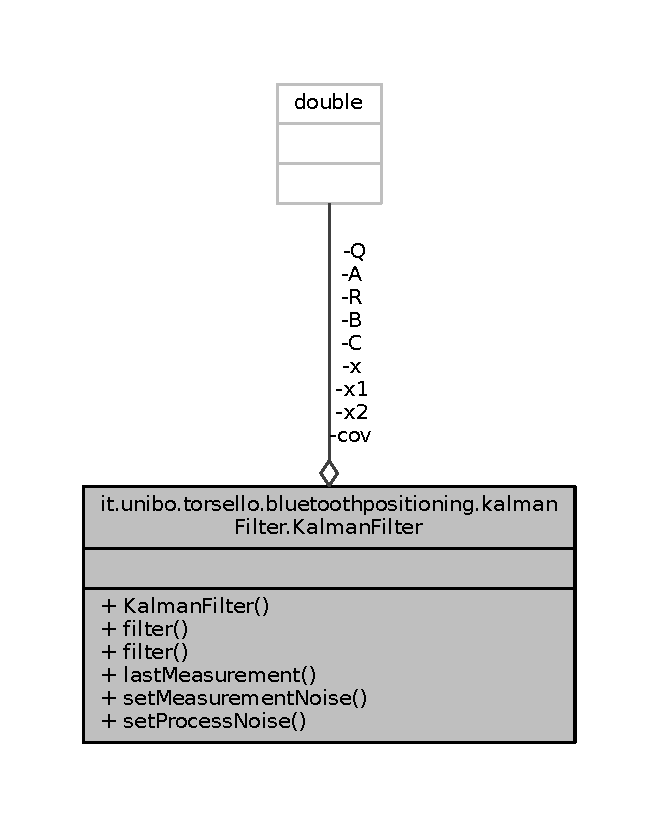
\includegraphics[width=316pt]{classit_1_1unibo_1_1torsello_1_1bluetoothpositioning_1_1kalmanFilter_1_1KalmanFilter__coll__graph}
\end{center}
\end{figure}
\subsubsection*{Membri pubblici}
\begin{DoxyCompactItemize}
\item 
\hyperlink{classit_1_1unibo_1_1torsello_1_1bluetoothpositioning_1_1kalmanFilter_1_1KalmanFilter_a9cbadb73c49c9d1e49776df4edca54f0_a9cbadb73c49c9d1e49776df4edca54f0}{Kalman\+Filter} (double \hyperlink{classit_1_1unibo_1_1torsello_1_1bluetoothpositioning_1_1kalmanFilter_1_1KalmanFilter_ad9b73500bbbee6969b5cfbe1a6e7a5ab_ad9b73500bbbee6969b5cfbe1a6e7a5ab}{R}, double \hyperlink{classit_1_1unibo_1_1torsello_1_1bluetoothpositioning_1_1kalmanFilter_1_1KalmanFilter_a684136c1ebc53dab2d661e98e7485a0a_a684136c1ebc53dab2d661e98e7485a0a}{Q}, double \hyperlink{classit_1_1unibo_1_1torsello_1_1bluetoothpositioning_1_1kalmanFilter_1_1KalmanFilter_a5222a1da9d5ef7f961a870402a245c06_a5222a1da9d5ef7f961a870402a245c06}{A}, double \hyperlink{classit_1_1unibo_1_1torsello_1_1bluetoothpositioning_1_1kalmanFilter_1_1KalmanFilter_a50cc9b19f576bafde991715386e35f14_a50cc9b19f576bafde991715386e35f14}{B}, double \hyperlink{classit_1_1unibo_1_1torsello_1_1bluetoothpositioning_1_1kalmanFilter_1_1KalmanFilter_a0e605eaeec6a8d59254d45a6bbef2a52_a0e605eaeec6a8d59254d45a6bbef2a52}{C})
\item 
double \hyperlink{classit_1_1unibo_1_1torsello_1_1bluetoothpositioning_1_1kalmanFilter_1_1KalmanFilter_add00ee8814dc3f7692db79ecb18b030c_add00ee8814dc3f7692db79ecb18b030c}{filter} (double z)
\item 
double \hyperlink{classit_1_1unibo_1_1torsello_1_1bluetoothpositioning_1_1kalmanFilter_1_1KalmanFilter_ab50a6f6e395f63d2b581fbcbf3742c57_ab50a6f6e395f63d2b581fbcbf3742c57}{filter} (double z, double u)
\item 
double \hyperlink{classit_1_1unibo_1_1torsello_1_1bluetoothpositioning_1_1kalmanFilter_1_1KalmanFilter_a43184e14be498b5a7fb684f6713a9697_a43184e14be498b5a7fb684f6713a9697}{last\+Measurement} ()
\item 
void \hyperlink{classit_1_1unibo_1_1torsello_1_1bluetoothpositioning_1_1kalmanFilter_1_1KalmanFilter_a320315e589b1908f604745e1381c8710_a320315e589b1908f604745e1381c8710}{set\+Measurement\+Noise} (double noise)
\item 
void \hyperlink{classit_1_1unibo_1_1torsello_1_1bluetoothpositioning_1_1kalmanFilter_1_1KalmanFilter_ad8c1946d417c0b8b1991228ffa02bdd6_ad8c1946d417c0b8b1991228ffa02bdd6}{set\+Process\+Noise} (double noise)
\end{DoxyCompactItemize}
\subsubsection*{Attributi privati}
\begin{DoxyCompactItemize}
\item 
double \hyperlink{classit_1_1unibo_1_1torsello_1_1bluetoothpositioning_1_1kalmanFilter_1_1KalmanFilter_ad9b73500bbbee6969b5cfbe1a6e7a5ab_ad9b73500bbbee6969b5cfbe1a6e7a5ab}{R}
\item 
double \hyperlink{classit_1_1unibo_1_1torsello_1_1bluetoothpositioning_1_1kalmanFilter_1_1KalmanFilter_a684136c1ebc53dab2d661e98e7485a0a_a684136c1ebc53dab2d661e98e7485a0a}{Q}
\item 
double \hyperlink{classit_1_1unibo_1_1torsello_1_1bluetoothpositioning_1_1kalmanFilter_1_1KalmanFilter_a5222a1da9d5ef7f961a870402a245c06_a5222a1da9d5ef7f961a870402a245c06}{A}
\item 
double \hyperlink{classit_1_1unibo_1_1torsello_1_1bluetoothpositioning_1_1kalmanFilter_1_1KalmanFilter_a50cc9b19f576bafde991715386e35f14_a50cc9b19f576bafde991715386e35f14}{B}
\item 
double \hyperlink{classit_1_1unibo_1_1torsello_1_1bluetoothpositioning_1_1kalmanFilter_1_1KalmanFilter_a0e605eaeec6a8d59254d45a6bbef2a52_a0e605eaeec6a8d59254d45a6bbef2a52}{C}
\item 
double \hyperlink{classit_1_1unibo_1_1torsello_1_1bluetoothpositioning_1_1kalmanFilter_1_1KalmanFilter_a9446f9ad4fbe8b2665e8109c9a22758e_a9446f9ad4fbe8b2665e8109c9a22758e}{cov}
\item 
double \hyperlink{classit_1_1unibo_1_1torsello_1_1bluetoothpositioning_1_1kalmanFilter_1_1KalmanFilter_acab8f5b6d2cec6daae8c6e5a300243cd_acab8f5b6d2cec6daae8c6e5a300243cd}{x}
\item 
double \hyperlink{classit_1_1unibo_1_1torsello_1_1bluetoothpositioning_1_1kalmanFilter_1_1KalmanFilter_a3c6dc655806d5f59d57602cad9d3003a_a3c6dc655806d5f59d57602cad9d3003a}{x1}
\item 
double \hyperlink{classit_1_1unibo_1_1torsello_1_1bluetoothpositioning_1_1kalmanFilter_1_1KalmanFilter_a6f38c2ce61663eb8393cdb4e37fef427_a6f38c2ce61663eb8393cdb4e37fef427}{x2}
\end{DoxyCompactItemize}


\subsubsection{Descrizione dettagliata}
Originally written in JS by Wouter Bulten 2015 Rewritten to Java by Jonathan Vidmar 2016 Copyright 2015 Wouter Bulten G\+NU L\+E\+S\+S\+ER G\+E\+N\+E\+R\+AL P\+U\+B\+L\+IC L\+I\+C\+E\+N\+SE v3 

\subsubsection{Documentazione dei costruttori e dei distruttori}
\hypertarget{classit_1_1unibo_1_1torsello_1_1bluetoothpositioning_1_1kalmanFilter_1_1KalmanFilter_a9cbadb73c49c9d1e49776df4edca54f0_a9cbadb73c49c9d1e49776df4edca54f0}{}\label{classit_1_1unibo_1_1torsello_1_1bluetoothpositioning_1_1kalmanFilter_1_1KalmanFilter_a9cbadb73c49c9d1e49776df4edca54f0_a9cbadb73c49c9d1e49776df4edca54f0} 
\index{it\+::unibo\+::torsello\+::bluetoothpositioning\+::kalman\+Filter\+::\+Kalman\+Filter@{it\+::unibo\+::torsello\+::bluetoothpositioning\+::kalman\+Filter\+::\+Kalman\+Filter}!Kalman\+Filter@{Kalman\+Filter}}
\index{Kalman\+Filter@{Kalman\+Filter}!it\+::unibo\+::torsello\+::bluetoothpositioning\+::kalman\+Filter\+::\+Kalman\+Filter@{it\+::unibo\+::torsello\+::bluetoothpositioning\+::kalman\+Filter\+::\+Kalman\+Filter}}
\paragraph{\texorpdfstring{Kalman\+Filter()}{KalmanFilter()}}
{\footnotesize\ttfamily it.\+unibo.\+torsello.\+bluetoothpositioning.\+kalman\+Filter.\+Kalman\+Filter.\+Kalman\+Filter (\begin{DoxyParamCaption}\item[{double}]{R,  }\item[{double}]{Q,  }\item[{double}]{A,  }\item[{double}]{B,  }\item[{double}]{C }\end{DoxyParamCaption})}

Create 1-\/dimensional kalman filter


\begin{DoxyParams}{Parametri}
{\em R} & Process noise \\
\hline
{\em Q} & Measurement noise \\
\hline
{\em A} & State vector \\
\hline
{\em B} & Control vector \\
\hline
{\em C} & Measurement vector \\
\hline
\end{DoxyParams}

\begin{DoxyCode}
30                                                                           \{
31 
32         this.\hyperlink{classit_1_1unibo_1_1torsello_1_1bluetoothpositioning_1_1kalmanFilter_1_1KalmanFilter_ad9b73500bbbee6969b5cfbe1a6e7a5ab_ad9b73500bbbee6969b5cfbe1a6e7a5ab}{R} = \hyperlink{classit_1_1unibo_1_1torsello_1_1bluetoothpositioning_1_1kalmanFilter_1_1KalmanFilter_ad9b73500bbbee6969b5cfbe1a6e7a5ab_ad9b73500bbbee6969b5cfbe1a6e7a5ab}{R};
33         this.\hyperlink{classit_1_1unibo_1_1torsello_1_1bluetoothpositioning_1_1kalmanFilter_1_1KalmanFilter_a684136c1ebc53dab2d661e98e7485a0a_a684136c1ebc53dab2d661e98e7485a0a}{Q} = \hyperlink{classit_1_1unibo_1_1torsello_1_1bluetoothpositioning_1_1kalmanFilter_1_1KalmanFilter_a684136c1ebc53dab2d661e98e7485a0a_a684136c1ebc53dab2d661e98e7485a0a}{Q};
34         this.\hyperlink{classit_1_1unibo_1_1torsello_1_1bluetoothpositioning_1_1kalmanFilter_1_1KalmanFilter_a5222a1da9d5ef7f961a870402a245c06_a5222a1da9d5ef7f961a870402a245c06}{A} = \hyperlink{classit_1_1unibo_1_1torsello_1_1bluetoothpositioning_1_1kalmanFilter_1_1KalmanFilter_a5222a1da9d5ef7f961a870402a245c06_a5222a1da9d5ef7f961a870402a245c06}{A};
35         this.\hyperlink{classit_1_1unibo_1_1torsello_1_1bluetoothpositioning_1_1kalmanFilter_1_1KalmanFilter_a50cc9b19f576bafde991715386e35f14_a50cc9b19f576bafde991715386e35f14}{B} = \hyperlink{classit_1_1unibo_1_1torsello_1_1bluetoothpositioning_1_1kalmanFilter_1_1KalmanFilter_a50cc9b19f576bafde991715386e35f14_a50cc9b19f576bafde991715386e35f14}{B};
36         this.\hyperlink{classit_1_1unibo_1_1torsello_1_1bluetoothpositioning_1_1kalmanFilter_1_1KalmanFilter_a0e605eaeec6a8d59254d45a6bbef2a52_a0e605eaeec6a8d59254d45a6bbef2a52}{C} = \hyperlink{classit_1_1unibo_1_1torsello_1_1bluetoothpositioning_1_1kalmanFilter_1_1KalmanFilter_a0e605eaeec6a8d59254d45a6bbef2a52_a0e605eaeec6a8d59254d45a6bbef2a52}{C};
37 
38         \hyperlink{classit_1_1unibo_1_1torsello_1_1bluetoothpositioning_1_1kalmanFilter_1_1KalmanFilter_a9446f9ad4fbe8b2665e8109c9a22758e_a9446f9ad4fbe8b2665e8109c9a22758e}{cov} = Double.NaN;
39         \hyperlink{classit_1_1unibo_1_1torsello_1_1bluetoothpositioning_1_1kalmanFilter_1_1KalmanFilter_acab8f5b6d2cec6daae8c6e5a300243cd_acab8f5b6d2cec6daae8c6e5a300243cd}{x} = Double.NaN;
40     \}
\end{DoxyCode}


\subsubsection{Documentazione delle funzioni membro}
\hypertarget{classit_1_1unibo_1_1torsello_1_1bluetoothpositioning_1_1kalmanFilter_1_1KalmanFilter_add00ee8814dc3f7692db79ecb18b030c_add00ee8814dc3f7692db79ecb18b030c}{}\label{classit_1_1unibo_1_1torsello_1_1bluetoothpositioning_1_1kalmanFilter_1_1KalmanFilter_add00ee8814dc3f7692db79ecb18b030c_add00ee8814dc3f7692db79ecb18b030c} 
\index{it\+::unibo\+::torsello\+::bluetoothpositioning\+::kalman\+Filter\+::\+Kalman\+Filter@{it\+::unibo\+::torsello\+::bluetoothpositioning\+::kalman\+Filter\+::\+Kalman\+Filter}!filter@{filter}}
\index{filter@{filter}!it\+::unibo\+::torsello\+::bluetoothpositioning\+::kalman\+Filter\+::\+Kalman\+Filter@{it\+::unibo\+::torsello\+::bluetoothpositioning\+::kalman\+Filter\+::\+Kalman\+Filter}}
\paragraph{\texorpdfstring{filter()}{filter()}\hspace{0.1cm}{\footnotesize\ttfamily [1/2]}}
{\footnotesize\ttfamily double it.\+unibo.\+torsello.\+bluetoothpositioning.\+kalman\+Filter.\+Kalman\+Filter.\+filter (\begin{DoxyParamCaption}\item[{double}]{z }\end{DoxyParamCaption})}


\begin{DoxyCode}
43                                    \{
44         \textcolor{keywordflow}{return} \hyperlink{classit_1_1unibo_1_1torsello_1_1bluetoothpositioning_1_1kalmanFilter_1_1KalmanFilter_add00ee8814dc3f7692db79ecb18b030c_add00ee8814dc3f7692db79ecb18b030c}{filter}(z, 0);
45     \}
\end{DoxyCode}
\hypertarget{classit_1_1unibo_1_1torsello_1_1bluetoothpositioning_1_1kalmanFilter_1_1KalmanFilter_ab50a6f6e395f63d2b581fbcbf3742c57_ab50a6f6e395f63d2b581fbcbf3742c57}{}\label{classit_1_1unibo_1_1torsello_1_1bluetoothpositioning_1_1kalmanFilter_1_1KalmanFilter_ab50a6f6e395f63d2b581fbcbf3742c57_ab50a6f6e395f63d2b581fbcbf3742c57} 
\index{it\+::unibo\+::torsello\+::bluetoothpositioning\+::kalman\+Filter\+::\+Kalman\+Filter@{it\+::unibo\+::torsello\+::bluetoothpositioning\+::kalman\+Filter\+::\+Kalman\+Filter}!filter@{filter}}
\index{filter@{filter}!it\+::unibo\+::torsello\+::bluetoothpositioning\+::kalman\+Filter\+::\+Kalman\+Filter@{it\+::unibo\+::torsello\+::bluetoothpositioning\+::kalman\+Filter\+::\+Kalman\+Filter}}
\paragraph{\texorpdfstring{filter()}{filter()}\hspace{0.1cm}{\footnotesize\ttfamily [2/2]}}
{\footnotesize\ttfamily double it.\+unibo.\+torsello.\+bluetoothpositioning.\+kalman\+Filter.\+Kalman\+Filter.\+filter (\begin{DoxyParamCaption}\item[{double}]{z,  }\item[{double}]{u }\end{DoxyParamCaption})}

Filter a new value


\begin{DoxyParams}{Parametri}
{\em z} & Measurement \\
\hline
{\em u} & Control \\
\hline
\end{DoxyParams}
\begin{DoxyReturn}{Restituisce}
x 
\end{DoxyReturn}

\begin{DoxyCode}
54                                              \{
55 
56         \textcolor{keywordflow}{if} (Double.isNaN(\hyperlink{classit_1_1unibo_1_1torsello_1_1bluetoothpositioning_1_1kalmanFilter_1_1KalmanFilter_acab8f5b6d2cec6daae8c6e5a300243cd_acab8f5b6d2cec6daae8c6e5a300243cd}{x})) \{
57             \hyperlink{classit_1_1unibo_1_1torsello_1_1bluetoothpositioning_1_1kalmanFilter_1_1KalmanFilter_acab8f5b6d2cec6daae8c6e5a300243cd_acab8f5b6d2cec6daae8c6e5a300243cd}{x} = (1 / \hyperlink{classit_1_1unibo_1_1torsello_1_1bluetoothpositioning_1_1kalmanFilter_1_1KalmanFilter_a0e605eaeec6a8d59254d45a6bbef2a52_a0e605eaeec6a8d59254d45a6bbef2a52}{C}) * z;
58             \hyperlink{classit_1_1unibo_1_1torsello_1_1bluetoothpositioning_1_1kalmanFilter_1_1KalmanFilter_a3c6dc655806d5f59d57602cad9d3003a_a3c6dc655806d5f59d57602cad9d3003a}{x1} = \hyperlink{classit_1_1unibo_1_1torsello_1_1bluetoothpositioning_1_1kalmanFilter_1_1KalmanFilter_acab8f5b6d2cec6daae8c6e5a300243cd_acab8f5b6d2cec6daae8c6e5a300243cd}{x};
59             \hyperlink{classit_1_1unibo_1_1torsello_1_1bluetoothpositioning_1_1kalmanFilter_1_1KalmanFilter_a6f38c2ce61663eb8393cdb4e37fef427_a6f38c2ce61663eb8393cdb4e37fef427}{x2} = \hyperlink{classit_1_1unibo_1_1torsello_1_1bluetoothpositioning_1_1kalmanFilter_1_1KalmanFilter_a3c6dc655806d5f59d57602cad9d3003a_a3c6dc655806d5f59d57602cad9d3003a}{x1};
60             \hyperlink{classit_1_1unibo_1_1torsello_1_1bluetoothpositioning_1_1kalmanFilter_1_1KalmanFilter_a9446f9ad4fbe8b2665e8109c9a22758e_a9446f9ad4fbe8b2665e8109c9a22758e}{cov} = (1 / \hyperlink{classit_1_1unibo_1_1torsello_1_1bluetoothpositioning_1_1kalmanFilter_1_1KalmanFilter_a0e605eaeec6a8d59254d45a6bbef2a52_a0e605eaeec6a8d59254d45a6bbef2a52}{C}) * \hyperlink{classit_1_1unibo_1_1torsello_1_1bluetoothpositioning_1_1kalmanFilter_1_1KalmanFilter_a684136c1ebc53dab2d661e98e7485a0a_a684136c1ebc53dab2d661e98e7485a0a}{Q} * (1 / \hyperlink{classit_1_1unibo_1_1torsello_1_1bluetoothpositioning_1_1kalmanFilter_1_1KalmanFilter_a0e605eaeec6a8d59254d45a6bbef2a52_a0e605eaeec6a8d59254d45a6bbef2a52}{C});
61         \} \textcolor{keywordflow}{else} \{
62 
63             \textcolor{comment}{// Calculate previous update step}
64             \hyperlink{classit_1_1unibo_1_1torsello_1_1bluetoothpositioning_1_1kalmanFilter_1_1KalmanFilter_a50cc9b19f576bafde991715386e35f14_a50cc9b19f576bafde991715386e35f14}{B} = (\hyperlink{classit_1_1unibo_1_1torsello_1_1bluetoothpositioning_1_1kalmanFilter_1_1KalmanFilter_acab8f5b6d2cec6daae8c6e5a300243cd_acab8f5b6d2cec6daae8c6e5a300243cd}{x} - \hyperlink{classit_1_1unibo_1_1torsello_1_1bluetoothpositioning_1_1kalmanFilter_1_1KalmanFilter_a3c6dc655806d5f59d57602cad9d3003a_a3c6dc655806d5f59d57602cad9d3003a}{x1}) / 2;
65 
66             \textcolor{comment}{// Compute prediction}
67             \textcolor{keywordtype}{double} predX = (\hyperlink{classit_1_1unibo_1_1torsello_1_1bluetoothpositioning_1_1kalmanFilter_1_1KalmanFilter_a5222a1da9d5ef7f961a870402a245c06_a5222a1da9d5ef7f961a870402a245c06}{A} * \hyperlink{classit_1_1unibo_1_1torsello_1_1bluetoothpositioning_1_1kalmanFilter_1_1KalmanFilter_acab8f5b6d2cec6daae8c6e5a300243cd_acab8f5b6d2cec6daae8c6e5a300243cd}{x}) + (\hyperlink{classit_1_1unibo_1_1torsello_1_1bluetoothpositioning_1_1kalmanFilter_1_1KalmanFilter_a50cc9b19f576bafde991715386e35f14_a50cc9b19f576bafde991715386e35f14}{B} * u);
68             \textcolor{keywordtype}{double} predCov = ((\hyperlink{classit_1_1unibo_1_1torsello_1_1bluetoothpositioning_1_1kalmanFilter_1_1KalmanFilter_a5222a1da9d5ef7f961a870402a245c06_a5222a1da9d5ef7f961a870402a245c06}{A} * \hyperlink{classit_1_1unibo_1_1torsello_1_1bluetoothpositioning_1_1kalmanFilter_1_1KalmanFilter_a9446f9ad4fbe8b2665e8109c9a22758e_a9446f9ad4fbe8b2665e8109c9a22758e}{cov}) * \hyperlink{classit_1_1unibo_1_1torsello_1_1bluetoothpositioning_1_1kalmanFilter_1_1KalmanFilter_a5222a1da9d5ef7f961a870402a245c06_a5222a1da9d5ef7f961a870402a245c06}{A}) + \hyperlink{classit_1_1unibo_1_1torsello_1_1bluetoothpositioning_1_1kalmanFilter_1_1KalmanFilter_ad9b73500bbbee6969b5cfbe1a6e7a5ab_ad9b73500bbbee6969b5cfbe1a6e7a5ab}{R};
69 
70             \textcolor{comment}{// Kalman gain}
71             \textcolor{keywordtype}{double} K = predCov * \hyperlink{classit_1_1unibo_1_1torsello_1_1bluetoothpositioning_1_1kalmanFilter_1_1KalmanFilter_a0e605eaeec6a8d59254d45a6bbef2a52_a0e605eaeec6a8d59254d45a6bbef2a52}{C} * (1 / ((\hyperlink{classit_1_1unibo_1_1torsello_1_1bluetoothpositioning_1_1kalmanFilter_1_1KalmanFilter_a0e605eaeec6a8d59254d45a6bbef2a52_a0e605eaeec6a8d59254d45a6bbef2a52}{C} * predCov * \hyperlink{classit_1_1unibo_1_1torsello_1_1bluetoothpositioning_1_1kalmanFilter_1_1KalmanFilter_a0e605eaeec6a8d59254d45a6bbef2a52_a0e605eaeec6a8d59254d45a6bbef2a52}{C}) + \hyperlink{classit_1_1unibo_1_1torsello_1_1bluetoothpositioning_1_1kalmanFilter_1_1KalmanFilter_a684136c1ebc53dab2d661e98e7485a0a_a684136c1ebc53dab2d661e98e7485a0a}{Q}));
72 
73             \textcolor{comment}{// Correction}
74             \hyperlink{classit_1_1unibo_1_1torsello_1_1bluetoothpositioning_1_1kalmanFilter_1_1KalmanFilter_a3c6dc655806d5f59d57602cad9d3003a_a3c6dc655806d5f59d57602cad9d3003a}{x1} = \hyperlink{classit_1_1unibo_1_1torsello_1_1bluetoothpositioning_1_1kalmanFilter_1_1KalmanFilter_acab8f5b6d2cec6daae8c6e5a300243cd_acab8f5b6d2cec6daae8c6e5a300243cd}{x};
75             \hyperlink{classit_1_1unibo_1_1torsello_1_1bluetoothpositioning_1_1kalmanFilter_1_1KalmanFilter_acab8f5b6d2cec6daae8c6e5a300243cd_acab8f5b6d2cec6daae8c6e5a300243cd}{x} = predX + K * (z - (\hyperlink{classit_1_1unibo_1_1torsello_1_1bluetoothpositioning_1_1kalmanFilter_1_1KalmanFilter_a0e605eaeec6a8d59254d45a6bbef2a52_a0e605eaeec6a8d59254d45a6bbef2a52}{C} * predX));
76             \hyperlink{classit_1_1unibo_1_1torsello_1_1bluetoothpositioning_1_1kalmanFilter_1_1KalmanFilter_a9446f9ad4fbe8b2665e8109c9a22758e_a9446f9ad4fbe8b2665e8109c9a22758e}{cov} = predCov - (K * \hyperlink{classit_1_1unibo_1_1torsello_1_1bluetoothpositioning_1_1kalmanFilter_1_1KalmanFilter_a0e605eaeec6a8d59254d45a6bbef2a52_a0e605eaeec6a8d59254d45a6bbef2a52}{C} * predCov);
77         \}
78 
79         \textcolor{keywordflow}{return} \hyperlink{classit_1_1unibo_1_1torsello_1_1bluetoothpositioning_1_1kalmanFilter_1_1KalmanFilter_acab8f5b6d2cec6daae8c6e5a300243cd_acab8f5b6d2cec6daae8c6e5a300243cd}{x};
80     \}
\end{DoxyCode}
\hypertarget{classit_1_1unibo_1_1torsello_1_1bluetoothpositioning_1_1kalmanFilter_1_1KalmanFilter_a43184e14be498b5a7fb684f6713a9697_a43184e14be498b5a7fb684f6713a9697}{}\label{classit_1_1unibo_1_1torsello_1_1bluetoothpositioning_1_1kalmanFilter_1_1KalmanFilter_a43184e14be498b5a7fb684f6713a9697_a43184e14be498b5a7fb684f6713a9697} 
\index{it\+::unibo\+::torsello\+::bluetoothpositioning\+::kalman\+Filter\+::\+Kalman\+Filter@{it\+::unibo\+::torsello\+::bluetoothpositioning\+::kalman\+Filter\+::\+Kalman\+Filter}!last\+Measurement@{last\+Measurement}}
\index{last\+Measurement@{last\+Measurement}!it\+::unibo\+::torsello\+::bluetoothpositioning\+::kalman\+Filter\+::\+Kalman\+Filter@{it\+::unibo\+::torsello\+::bluetoothpositioning\+::kalman\+Filter\+::\+Kalman\+Filter}}
\paragraph{\texorpdfstring{last\+Measurement()}{lastMeasurement()}}
{\footnotesize\ttfamily double it.\+unibo.\+torsello.\+bluetoothpositioning.\+kalman\+Filter.\+Kalman\+Filter.\+last\+Measurement (\begin{DoxyParamCaption}{ }\end{DoxyParamCaption})}

Return the last filtered measurement

\begin{DoxyReturn}{Restituisce}
x Estimated signal without noise 
\end{DoxyReturn}

\begin{DoxyCode}
87                                     \{
88         \textcolor{keywordflow}{return} \hyperlink{classit_1_1unibo_1_1torsello_1_1bluetoothpositioning_1_1kalmanFilter_1_1KalmanFilter_acab8f5b6d2cec6daae8c6e5a300243cd_acab8f5b6d2cec6daae8c6e5a300243cd}{x};
89     \}
\end{DoxyCode}
\hypertarget{classit_1_1unibo_1_1torsello_1_1bluetoothpositioning_1_1kalmanFilter_1_1KalmanFilter_a320315e589b1908f604745e1381c8710_a320315e589b1908f604745e1381c8710}{}\label{classit_1_1unibo_1_1torsello_1_1bluetoothpositioning_1_1kalmanFilter_1_1KalmanFilter_a320315e589b1908f604745e1381c8710_a320315e589b1908f604745e1381c8710} 
\index{it\+::unibo\+::torsello\+::bluetoothpositioning\+::kalman\+Filter\+::\+Kalman\+Filter@{it\+::unibo\+::torsello\+::bluetoothpositioning\+::kalman\+Filter\+::\+Kalman\+Filter}!set\+Measurement\+Noise@{set\+Measurement\+Noise}}
\index{set\+Measurement\+Noise@{set\+Measurement\+Noise}!it\+::unibo\+::torsello\+::bluetoothpositioning\+::kalman\+Filter\+::\+Kalman\+Filter@{it\+::unibo\+::torsello\+::bluetoothpositioning\+::kalman\+Filter\+::\+Kalman\+Filter}}
\paragraph{\texorpdfstring{set\+Measurement\+Noise()}{setMeasurementNoise()}}
{\footnotesize\ttfamily void it.\+unibo.\+torsello.\+bluetoothpositioning.\+kalman\+Filter.\+Kalman\+Filter.\+set\+Measurement\+Noise (\begin{DoxyParamCaption}\item[{double}]{noise }\end{DoxyParamCaption})}

Set measurement noise Q


\begin{DoxyParams}{Parametri}
{\em noise} & Measurement noise \\
\hline
\end{DoxyParams}

\begin{DoxyCode}
96                                                   \{
97         \hyperlink{classit_1_1unibo_1_1torsello_1_1bluetoothpositioning_1_1kalmanFilter_1_1KalmanFilter_a684136c1ebc53dab2d661e98e7485a0a_a684136c1ebc53dab2d661e98e7485a0a}{Q} = noise;
98     \}
\end{DoxyCode}
\hypertarget{classit_1_1unibo_1_1torsello_1_1bluetoothpositioning_1_1kalmanFilter_1_1KalmanFilter_ad8c1946d417c0b8b1991228ffa02bdd6_ad8c1946d417c0b8b1991228ffa02bdd6}{}\label{classit_1_1unibo_1_1torsello_1_1bluetoothpositioning_1_1kalmanFilter_1_1KalmanFilter_ad8c1946d417c0b8b1991228ffa02bdd6_ad8c1946d417c0b8b1991228ffa02bdd6} 
\index{it\+::unibo\+::torsello\+::bluetoothpositioning\+::kalman\+Filter\+::\+Kalman\+Filter@{it\+::unibo\+::torsello\+::bluetoothpositioning\+::kalman\+Filter\+::\+Kalman\+Filter}!set\+Process\+Noise@{set\+Process\+Noise}}
\index{set\+Process\+Noise@{set\+Process\+Noise}!it\+::unibo\+::torsello\+::bluetoothpositioning\+::kalman\+Filter\+::\+Kalman\+Filter@{it\+::unibo\+::torsello\+::bluetoothpositioning\+::kalman\+Filter\+::\+Kalman\+Filter}}
\paragraph{\texorpdfstring{set\+Process\+Noise()}{setProcessNoise()}}
{\footnotesize\ttfamily void it.\+unibo.\+torsello.\+bluetoothpositioning.\+kalman\+Filter.\+Kalman\+Filter.\+set\+Process\+Noise (\begin{DoxyParamCaption}\item[{double}]{noise }\end{DoxyParamCaption})}

Set the process noise R


\begin{DoxyParams}{Parametri}
{\em noise} & Process noise \\
\hline
\end{DoxyParams}

\begin{DoxyCode}
105                                               \{
106         \hyperlink{classit_1_1unibo_1_1torsello_1_1bluetoothpositioning_1_1kalmanFilter_1_1KalmanFilter_ad9b73500bbbee6969b5cfbe1a6e7a5ab_ad9b73500bbbee6969b5cfbe1a6e7a5ab}{R} = noise;
107     \}
\end{DoxyCode}


\subsubsection{Documentazione dei membri dato}
\hypertarget{classit_1_1unibo_1_1torsello_1_1bluetoothpositioning_1_1kalmanFilter_1_1KalmanFilter_a5222a1da9d5ef7f961a870402a245c06_a5222a1da9d5ef7f961a870402a245c06}{}\label{classit_1_1unibo_1_1torsello_1_1bluetoothpositioning_1_1kalmanFilter_1_1KalmanFilter_a5222a1da9d5ef7f961a870402a245c06_a5222a1da9d5ef7f961a870402a245c06} 
\index{it\+::unibo\+::torsello\+::bluetoothpositioning\+::kalman\+Filter\+::\+Kalman\+Filter@{it\+::unibo\+::torsello\+::bluetoothpositioning\+::kalman\+Filter\+::\+Kalman\+Filter}!A@{A}}
\index{A@{A}!it\+::unibo\+::torsello\+::bluetoothpositioning\+::kalman\+Filter\+::\+Kalman\+Filter@{it\+::unibo\+::torsello\+::bluetoothpositioning\+::kalman\+Filter\+::\+Kalman\+Filter}}
\paragraph{\texorpdfstring{A}{A}}
{\footnotesize\ttfamily double it.\+unibo.\+torsello.\+bluetoothpositioning.\+kalman\+Filter.\+Kalman\+Filter.\+A\hspace{0.3cm}{\ttfamily [private]}}

\hypertarget{classit_1_1unibo_1_1torsello_1_1bluetoothpositioning_1_1kalmanFilter_1_1KalmanFilter_a50cc9b19f576bafde991715386e35f14_a50cc9b19f576bafde991715386e35f14}{}\label{classit_1_1unibo_1_1torsello_1_1bluetoothpositioning_1_1kalmanFilter_1_1KalmanFilter_a50cc9b19f576bafde991715386e35f14_a50cc9b19f576bafde991715386e35f14} 
\index{it\+::unibo\+::torsello\+::bluetoothpositioning\+::kalman\+Filter\+::\+Kalman\+Filter@{it\+::unibo\+::torsello\+::bluetoothpositioning\+::kalman\+Filter\+::\+Kalman\+Filter}!B@{B}}
\index{B@{B}!it\+::unibo\+::torsello\+::bluetoothpositioning\+::kalman\+Filter\+::\+Kalman\+Filter@{it\+::unibo\+::torsello\+::bluetoothpositioning\+::kalman\+Filter\+::\+Kalman\+Filter}}
\paragraph{\texorpdfstring{B}{B}}
{\footnotesize\ttfamily double it.\+unibo.\+torsello.\+bluetoothpositioning.\+kalman\+Filter.\+Kalman\+Filter.\+B\hspace{0.3cm}{\ttfamily [private]}}

\hypertarget{classit_1_1unibo_1_1torsello_1_1bluetoothpositioning_1_1kalmanFilter_1_1KalmanFilter_a0e605eaeec6a8d59254d45a6bbef2a52_a0e605eaeec6a8d59254d45a6bbef2a52}{}\label{classit_1_1unibo_1_1torsello_1_1bluetoothpositioning_1_1kalmanFilter_1_1KalmanFilter_a0e605eaeec6a8d59254d45a6bbef2a52_a0e605eaeec6a8d59254d45a6bbef2a52} 
\index{it\+::unibo\+::torsello\+::bluetoothpositioning\+::kalman\+Filter\+::\+Kalman\+Filter@{it\+::unibo\+::torsello\+::bluetoothpositioning\+::kalman\+Filter\+::\+Kalman\+Filter}!C@{C}}
\index{C@{C}!it\+::unibo\+::torsello\+::bluetoothpositioning\+::kalman\+Filter\+::\+Kalman\+Filter@{it\+::unibo\+::torsello\+::bluetoothpositioning\+::kalman\+Filter\+::\+Kalman\+Filter}}
\paragraph{\texorpdfstring{C}{C}}
{\footnotesize\ttfamily double it.\+unibo.\+torsello.\+bluetoothpositioning.\+kalman\+Filter.\+Kalman\+Filter.\+C\hspace{0.3cm}{\ttfamily [private]}}

\hypertarget{classit_1_1unibo_1_1torsello_1_1bluetoothpositioning_1_1kalmanFilter_1_1KalmanFilter_a9446f9ad4fbe8b2665e8109c9a22758e_a9446f9ad4fbe8b2665e8109c9a22758e}{}\label{classit_1_1unibo_1_1torsello_1_1bluetoothpositioning_1_1kalmanFilter_1_1KalmanFilter_a9446f9ad4fbe8b2665e8109c9a22758e_a9446f9ad4fbe8b2665e8109c9a22758e} 
\index{it\+::unibo\+::torsello\+::bluetoothpositioning\+::kalman\+Filter\+::\+Kalman\+Filter@{it\+::unibo\+::torsello\+::bluetoothpositioning\+::kalman\+Filter\+::\+Kalman\+Filter}!cov@{cov}}
\index{cov@{cov}!it\+::unibo\+::torsello\+::bluetoothpositioning\+::kalman\+Filter\+::\+Kalman\+Filter@{it\+::unibo\+::torsello\+::bluetoothpositioning\+::kalman\+Filter\+::\+Kalman\+Filter}}
\paragraph{\texorpdfstring{cov}{cov}}
{\footnotesize\ttfamily double it.\+unibo.\+torsello.\+bluetoothpositioning.\+kalman\+Filter.\+Kalman\+Filter.\+cov\hspace{0.3cm}{\ttfamily [private]}}

\hypertarget{classit_1_1unibo_1_1torsello_1_1bluetoothpositioning_1_1kalmanFilter_1_1KalmanFilter_a684136c1ebc53dab2d661e98e7485a0a_a684136c1ebc53dab2d661e98e7485a0a}{}\label{classit_1_1unibo_1_1torsello_1_1bluetoothpositioning_1_1kalmanFilter_1_1KalmanFilter_a684136c1ebc53dab2d661e98e7485a0a_a684136c1ebc53dab2d661e98e7485a0a} 
\index{it\+::unibo\+::torsello\+::bluetoothpositioning\+::kalman\+Filter\+::\+Kalman\+Filter@{it\+::unibo\+::torsello\+::bluetoothpositioning\+::kalman\+Filter\+::\+Kalman\+Filter}!Q@{Q}}
\index{Q@{Q}!it\+::unibo\+::torsello\+::bluetoothpositioning\+::kalman\+Filter\+::\+Kalman\+Filter@{it\+::unibo\+::torsello\+::bluetoothpositioning\+::kalman\+Filter\+::\+Kalman\+Filter}}
\paragraph{\texorpdfstring{Q}{Q}}
{\footnotesize\ttfamily double it.\+unibo.\+torsello.\+bluetoothpositioning.\+kalman\+Filter.\+Kalman\+Filter.\+Q\hspace{0.3cm}{\ttfamily [private]}}

\hypertarget{classit_1_1unibo_1_1torsello_1_1bluetoothpositioning_1_1kalmanFilter_1_1KalmanFilter_ad9b73500bbbee6969b5cfbe1a6e7a5ab_ad9b73500bbbee6969b5cfbe1a6e7a5ab}{}\label{classit_1_1unibo_1_1torsello_1_1bluetoothpositioning_1_1kalmanFilter_1_1KalmanFilter_ad9b73500bbbee6969b5cfbe1a6e7a5ab_ad9b73500bbbee6969b5cfbe1a6e7a5ab} 
\index{it\+::unibo\+::torsello\+::bluetoothpositioning\+::kalman\+Filter\+::\+Kalman\+Filter@{it\+::unibo\+::torsello\+::bluetoothpositioning\+::kalman\+Filter\+::\+Kalman\+Filter}!R@{R}}
\index{R@{R}!it\+::unibo\+::torsello\+::bluetoothpositioning\+::kalman\+Filter\+::\+Kalman\+Filter@{it\+::unibo\+::torsello\+::bluetoothpositioning\+::kalman\+Filter\+::\+Kalman\+Filter}}
\paragraph{\texorpdfstring{R}{R}}
{\footnotesize\ttfamily double it.\+unibo.\+torsello.\+bluetoothpositioning.\+kalman\+Filter.\+Kalman\+Filter.\+R\hspace{0.3cm}{\ttfamily [private]}}

\hypertarget{classit_1_1unibo_1_1torsello_1_1bluetoothpositioning_1_1kalmanFilter_1_1KalmanFilter_acab8f5b6d2cec6daae8c6e5a300243cd_acab8f5b6d2cec6daae8c6e5a300243cd}{}\label{classit_1_1unibo_1_1torsello_1_1bluetoothpositioning_1_1kalmanFilter_1_1KalmanFilter_acab8f5b6d2cec6daae8c6e5a300243cd_acab8f5b6d2cec6daae8c6e5a300243cd} 
\index{it\+::unibo\+::torsello\+::bluetoothpositioning\+::kalman\+Filter\+::\+Kalman\+Filter@{it\+::unibo\+::torsello\+::bluetoothpositioning\+::kalman\+Filter\+::\+Kalman\+Filter}!x@{x}}
\index{x@{x}!it\+::unibo\+::torsello\+::bluetoothpositioning\+::kalman\+Filter\+::\+Kalman\+Filter@{it\+::unibo\+::torsello\+::bluetoothpositioning\+::kalman\+Filter\+::\+Kalman\+Filter}}
\paragraph{\texorpdfstring{x}{x}}
{\footnotesize\ttfamily double it.\+unibo.\+torsello.\+bluetoothpositioning.\+kalman\+Filter.\+Kalman\+Filter.\+x\hspace{0.3cm}{\ttfamily [private]}}

\hypertarget{classit_1_1unibo_1_1torsello_1_1bluetoothpositioning_1_1kalmanFilter_1_1KalmanFilter_a3c6dc655806d5f59d57602cad9d3003a_a3c6dc655806d5f59d57602cad9d3003a}{}\label{classit_1_1unibo_1_1torsello_1_1bluetoothpositioning_1_1kalmanFilter_1_1KalmanFilter_a3c6dc655806d5f59d57602cad9d3003a_a3c6dc655806d5f59d57602cad9d3003a} 
\index{it\+::unibo\+::torsello\+::bluetoothpositioning\+::kalman\+Filter\+::\+Kalman\+Filter@{it\+::unibo\+::torsello\+::bluetoothpositioning\+::kalman\+Filter\+::\+Kalman\+Filter}!x1@{x1}}
\index{x1@{x1}!it\+::unibo\+::torsello\+::bluetoothpositioning\+::kalman\+Filter\+::\+Kalman\+Filter@{it\+::unibo\+::torsello\+::bluetoothpositioning\+::kalman\+Filter\+::\+Kalman\+Filter}}
\paragraph{\texorpdfstring{x1}{x1}}
{\footnotesize\ttfamily double it.\+unibo.\+torsello.\+bluetoothpositioning.\+kalman\+Filter.\+Kalman\+Filter.\+x1\hspace{0.3cm}{\ttfamily [private]}}

\hypertarget{classit_1_1unibo_1_1torsello_1_1bluetoothpositioning_1_1kalmanFilter_1_1KalmanFilter_a6f38c2ce61663eb8393cdb4e37fef427_a6f38c2ce61663eb8393cdb4e37fef427}{}\label{classit_1_1unibo_1_1torsello_1_1bluetoothpositioning_1_1kalmanFilter_1_1KalmanFilter_a6f38c2ce61663eb8393cdb4e37fef427_a6f38c2ce61663eb8393cdb4e37fef427} 
\index{it\+::unibo\+::torsello\+::bluetoothpositioning\+::kalman\+Filter\+::\+Kalman\+Filter@{it\+::unibo\+::torsello\+::bluetoothpositioning\+::kalman\+Filter\+::\+Kalman\+Filter}!x2@{x2}}
\index{x2@{x2}!it\+::unibo\+::torsello\+::bluetoothpositioning\+::kalman\+Filter\+::\+Kalman\+Filter@{it\+::unibo\+::torsello\+::bluetoothpositioning\+::kalman\+Filter\+::\+Kalman\+Filter}}
\paragraph{\texorpdfstring{x2}{x2}}
{\footnotesize\ttfamily double it.\+unibo.\+torsello.\+bluetoothpositioning.\+kalman\+Filter.\+Kalman\+Filter.\+x2\hspace{0.3cm}{\ttfamily [private]}}



La documentazione per questa classe è stata generata a partire dal seguente file\+:\begin{DoxyCompactItemize}
\item 
\hyperlink{KalmanFilter_8java}{Kalman\+Filter.\+java}\end{DoxyCompactItemize}

\hypertarget{classit_1_1unibo_1_1torsello_1_1bluetoothpositioning_1_1kalmanFilter_1_1KFBuilder}{}\subsection{Riferimenti per la classe it.\+unibo.\+torsello.\+bluetoothpositioning.\+kalman\+Filter.\+K\+F\+Builder}
\label{classit_1_1unibo_1_1torsello_1_1bluetoothpositioning_1_1kalmanFilter_1_1KFBuilder}\index{it.\+unibo.\+torsello.\+bluetoothpositioning.\+kalman\+Filter.\+K\+F\+Builder@{it.\+unibo.\+torsello.\+bluetoothpositioning.\+kalman\+Filter.\+K\+F\+Builder}}


Diagramma di collaborazione per it.\+unibo.\+torsello.\+bluetoothpositioning.\+kalman\+Filter.\+K\+F\+Builder\+:
\nopagebreak
\begin{figure}[H]
\begin{center}
\leavevmode
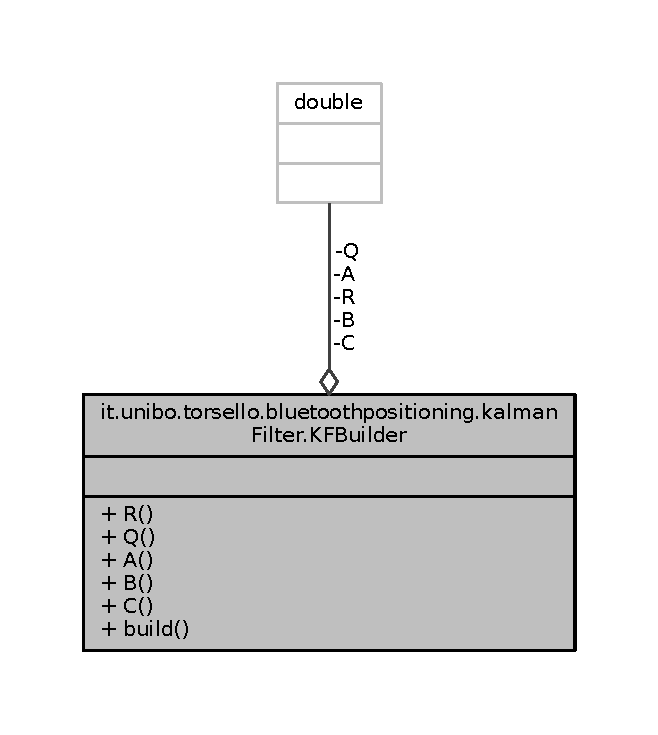
\includegraphics[width=316pt]{classit_1_1unibo_1_1torsello_1_1bluetoothpositioning_1_1kalmanFilter_1_1KFBuilder__coll__graph}
\end{center}
\end{figure}
\subsubsection*{Membri pubblici}
\begin{DoxyCompactItemize}
\item 
\hyperlink{classit_1_1unibo_1_1torsello_1_1bluetoothpositioning_1_1kalmanFilter_1_1KFBuilder}{K\+F\+Builder} \hyperlink{classit_1_1unibo_1_1torsello_1_1bluetoothpositioning_1_1kalmanFilter_1_1KFBuilder_ab356dae26769fa3dfe51dbaa480d5b2c_ab356dae26769fa3dfe51dbaa480d5b2c}{R} (double R)
\item 
\hyperlink{classit_1_1unibo_1_1torsello_1_1bluetoothpositioning_1_1kalmanFilter_1_1KFBuilder}{K\+F\+Builder} \hyperlink{classit_1_1unibo_1_1torsello_1_1bluetoothpositioning_1_1kalmanFilter_1_1KFBuilder_a4c11cae1419a47a25f94575d337d4c43_a4c11cae1419a47a25f94575d337d4c43}{Q} (double Q)
\item 
\hyperlink{classit_1_1unibo_1_1torsello_1_1bluetoothpositioning_1_1kalmanFilter_1_1KFBuilder}{K\+F\+Builder} \hyperlink{classit_1_1unibo_1_1torsello_1_1bluetoothpositioning_1_1kalmanFilter_1_1KFBuilder_a6b994b0e818818c6da83ab5448caf6b0_a6b994b0e818818c6da83ab5448caf6b0}{A} (double A)
\item 
\hyperlink{classit_1_1unibo_1_1torsello_1_1bluetoothpositioning_1_1kalmanFilter_1_1KFBuilder}{K\+F\+Builder} \hyperlink{classit_1_1unibo_1_1torsello_1_1bluetoothpositioning_1_1kalmanFilter_1_1KFBuilder_aea73a0f86bc40ea3d240620d04f25df7_aea73a0f86bc40ea3d240620d04f25df7}{B} (double B)
\item 
\hyperlink{classit_1_1unibo_1_1torsello_1_1bluetoothpositioning_1_1kalmanFilter_1_1KFBuilder}{K\+F\+Builder} \hyperlink{classit_1_1unibo_1_1torsello_1_1bluetoothpositioning_1_1kalmanFilter_1_1KFBuilder_ab86f143643d2f2d2e8aa78a42441db5a_ab86f143643d2f2d2e8aa78a42441db5a}{C} (double C)
\item 
\hyperlink{classit_1_1unibo_1_1torsello_1_1bluetoothpositioning_1_1kalmanFilter_1_1KalmanFilter}{Kalman\+Filter} \hyperlink{classit_1_1unibo_1_1torsello_1_1bluetoothpositioning_1_1kalmanFilter_1_1KFBuilder_ac4ac30ce0fabe2bf72a54ae1b737f587_ac4ac30ce0fabe2bf72a54ae1b737f587}{build} ()
\end{DoxyCompactItemize}
\subsubsection*{Attributi privati}
\begin{DoxyCompactItemize}
\item 
double \hyperlink{classit_1_1unibo_1_1torsello_1_1bluetoothpositioning_1_1kalmanFilter_1_1KFBuilder_a7937e1ec71fbede97b0bd70ead2e30dd_a7937e1ec71fbede97b0bd70ead2e30dd}{R} = 1
\item 
double \hyperlink{classit_1_1unibo_1_1torsello_1_1bluetoothpositioning_1_1kalmanFilter_1_1KFBuilder_ad332fe3c9e6ec20badaa4b8738fe264b_ad332fe3c9e6ec20badaa4b8738fe264b}{Q} = 1
\item 
double \hyperlink{classit_1_1unibo_1_1torsello_1_1bluetoothpositioning_1_1kalmanFilter_1_1KFBuilder_a89f12916414e352fc820a2c82fde76b8_a89f12916414e352fc820a2c82fde76b8}{A} = 1
\item 
double \hyperlink{classit_1_1unibo_1_1torsello_1_1bluetoothpositioning_1_1kalmanFilter_1_1KFBuilder_a0659c3648f664458d627741edf1de5a4_a0659c3648f664458d627741edf1de5a4}{B} = 0
\item 
double \hyperlink{classit_1_1unibo_1_1torsello_1_1bluetoothpositioning_1_1kalmanFilter_1_1KFBuilder_aa35dc81cfdbcef5286f8c812f1849341_aa35dc81cfdbcef5286f8c812f1849341}{C} = 1
\end{DoxyCompactItemize}


\subsubsection{Descrizione dettagliata}
Simple builder class for 1-\/dimensional Kalman filter with predefined 

\subsubsection{Documentazione delle funzioni membro}
\hypertarget{classit_1_1unibo_1_1torsello_1_1bluetoothpositioning_1_1kalmanFilter_1_1KFBuilder_a6b994b0e818818c6da83ab5448caf6b0_a6b994b0e818818c6da83ab5448caf6b0}{}\label{classit_1_1unibo_1_1torsello_1_1bluetoothpositioning_1_1kalmanFilter_1_1KFBuilder_a6b994b0e818818c6da83ab5448caf6b0_a6b994b0e818818c6da83ab5448caf6b0} 
\index{it\+::unibo\+::torsello\+::bluetoothpositioning\+::kalman\+Filter\+::\+K\+F\+Builder@{it\+::unibo\+::torsello\+::bluetoothpositioning\+::kalman\+Filter\+::\+K\+F\+Builder}!A@{A}}
\index{A@{A}!it\+::unibo\+::torsello\+::bluetoothpositioning\+::kalman\+Filter\+::\+K\+F\+Builder@{it\+::unibo\+::torsello\+::bluetoothpositioning\+::kalman\+Filter\+::\+K\+F\+Builder}}
\paragraph{\texorpdfstring{A()}{A()}}
{\footnotesize\ttfamily \hyperlink{classit_1_1unibo_1_1torsello_1_1bluetoothpositioning_1_1kalmanFilter_1_1KFBuilder}{K\+F\+Builder} it.\+unibo.\+torsello.\+bluetoothpositioning.\+kalman\+Filter.\+K\+F\+Builder.\+A (\begin{DoxyParamCaption}\item[{double}]{A }\end{DoxyParamCaption})}


\begin{DoxyCode}
23                                  \{
24         this.\hyperlink{classit_1_1unibo_1_1torsello_1_1bluetoothpositioning_1_1kalmanFilter_1_1KFBuilder_a89f12916414e352fc820a2c82fde76b8_a89f12916414e352fc820a2c82fde76b8}{A} = \hyperlink{classit_1_1unibo_1_1torsello_1_1bluetoothpositioning_1_1kalmanFilter_1_1KFBuilder_a89f12916414e352fc820a2c82fde76b8_a89f12916414e352fc820a2c82fde76b8}{A};
25         \textcolor{keywordflow}{return} \textcolor{keyword}{this};
26     \}
\end{DoxyCode}
\hypertarget{classit_1_1unibo_1_1torsello_1_1bluetoothpositioning_1_1kalmanFilter_1_1KFBuilder_aea73a0f86bc40ea3d240620d04f25df7_aea73a0f86bc40ea3d240620d04f25df7}{}\label{classit_1_1unibo_1_1torsello_1_1bluetoothpositioning_1_1kalmanFilter_1_1KFBuilder_aea73a0f86bc40ea3d240620d04f25df7_aea73a0f86bc40ea3d240620d04f25df7} 
\index{it\+::unibo\+::torsello\+::bluetoothpositioning\+::kalman\+Filter\+::\+K\+F\+Builder@{it\+::unibo\+::torsello\+::bluetoothpositioning\+::kalman\+Filter\+::\+K\+F\+Builder}!B@{B}}
\index{B@{B}!it\+::unibo\+::torsello\+::bluetoothpositioning\+::kalman\+Filter\+::\+K\+F\+Builder@{it\+::unibo\+::torsello\+::bluetoothpositioning\+::kalman\+Filter\+::\+K\+F\+Builder}}
\paragraph{\texorpdfstring{B()}{B()}}
{\footnotesize\ttfamily \hyperlink{classit_1_1unibo_1_1torsello_1_1bluetoothpositioning_1_1kalmanFilter_1_1KFBuilder}{K\+F\+Builder} it.\+unibo.\+torsello.\+bluetoothpositioning.\+kalman\+Filter.\+K\+F\+Builder.\+B (\begin{DoxyParamCaption}\item[{double}]{B }\end{DoxyParamCaption})}


\begin{DoxyCode}
28                                  \{
29         this.\hyperlink{classit_1_1unibo_1_1torsello_1_1bluetoothpositioning_1_1kalmanFilter_1_1KFBuilder_a0659c3648f664458d627741edf1de5a4_a0659c3648f664458d627741edf1de5a4}{B} = \hyperlink{classit_1_1unibo_1_1torsello_1_1bluetoothpositioning_1_1kalmanFilter_1_1KFBuilder_a0659c3648f664458d627741edf1de5a4_a0659c3648f664458d627741edf1de5a4}{B};
30         \textcolor{keywordflow}{return} \textcolor{keyword}{this};
31     \}
\end{DoxyCode}
\hypertarget{classit_1_1unibo_1_1torsello_1_1bluetoothpositioning_1_1kalmanFilter_1_1KFBuilder_ac4ac30ce0fabe2bf72a54ae1b737f587_ac4ac30ce0fabe2bf72a54ae1b737f587}{}\label{classit_1_1unibo_1_1torsello_1_1bluetoothpositioning_1_1kalmanFilter_1_1KFBuilder_ac4ac30ce0fabe2bf72a54ae1b737f587_ac4ac30ce0fabe2bf72a54ae1b737f587} 
\index{it\+::unibo\+::torsello\+::bluetoothpositioning\+::kalman\+Filter\+::\+K\+F\+Builder@{it\+::unibo\+::torsello\+::bluetoothpositioning\+::kalman\+Filter\+::\+K\+F\+Builder}!build@{build}}
\index{build@{build}!it\+::unibo\+::torsello\+::bluetoothpositioning\+::kalman\+Filter\+::\+K\+F\+Builder@{it\+::unibo\+::torsello\+::bluetoothpositioning\+::kalman\+Filter\+::\+K\+F\+Builder}}
\paragraph{\texorpdfstring{build()}{build()}}
{\footnotesize\ttfamily \hyperlink{classit_1_1unibo_1_1torsello_1_1bluetoothpositioning_1_1kalmanFilter_1_1KalmanFilter}{Kalman\+Filter} it.\+unibo.\+torsello.\+bluetoothpositioning.\+kalman\+Filter.\+K\+F\+Builder.\+build (\begin{DoxyParamCaption}{ }\end{DoxyParamCaption})}


\begin{DoxyCode}
38                                 \{
39         \textcolor{keywordflow}{return} \textcolor{keyword}{new} KalmanFilter(\hyperlink{classit_1_1unibo_1_1torsello_1_1bluetoothpositioning_1_1kalmanFilter_1_1KFBuilder_a7937e1ec71fbede97b0bd70ead2e30dd_a7937e1ec71fbede97b0bd70ead2e30dd}{R}, \hyperlink{classit_1_1unibo_1_1torsello_1_1bluetoothpositioning_1_1kalmanFilter_1_1KFBuilder_ad332fe3c9e6ec20badaa4b8738fe264b_ad332fe3c9e6ec20badaa4b8738fe264b}{Q}, \hyperlink{classit_1_1unibo_1_1torsello_1_1bluetoothpositioning_1_1kalmanFilter_1_1KFBuilder_a89f12916414e352fc820a2c82fde76b8_a89f12916414e352fc820a2c82fde76b8}{A}, \hyperlink{classit_1_1unibo_1_1torsello_1_1bluetoothpositioning_1_1kalmanFilter_1_1KFBuilder_a0659c3648f664458d627741edf1de5a4_a0659c3648f664458d627741edf1de5a4}{B}, \hyperlink{classit_1_1unibo_1_1torsello_1_1bluetoothpositioning_1_1kalmanFilter_1_1KFBuilder_aa35dc81cfdbcef5286f8c812f1849341_aa35dc81cfdbcef5286f8c812f1849341}{C});
40     \}
\end{DoxyCode}
\hypertarget{classit_1_1unibo_1_1torsello_1_1bluetoothpositioning_1_1kalmanFilter_1_1KFBuilder_ab86f143643d2f2d2e8aa78a42441db5a_ab86f143643d2f2d2e8aa78a42441db5a}{}\label{classit_1_1unibo_1_1torsello_1_1bluetoothpositioning_1_1kalmanFilter_1_1KFBuilder_ab86f143643d2f2d2e8aa78a42441db5a_ab86f143643d2f2d2e8aa78a42441db5a} 
\index{it\+::unibo\+::torsello\+::bluetoothpositioning\+::kalman\+Filter\+::\+K\+F\+Builder@{it\+::unibo\+::torsello\+::bluetoothpositioning\+::kalman\+Filter\+::\+K\+F\+Builder}!C@{C}}
\index{C@{C}!it\+::unibo\+::torsello\+::bluetoothpositioning\+::kalman\+Filter\+::\+K\+F\+Builder@{it\+::unibo\+::torsello\+::bluetoothpositioning\+::kalman\+Filter\+::\+K\+F\+Builder}}
\paragraph{\texorpdfstring{C()}{C()}}
{\footnotesize\ttfamily \hyperlink{classit_1_1unibo_1_1torsello_1_1bluetoothpositioning_1_1kalmanFilter_1_1KFBuilder}{K\+F\+Builder} it.\+unibo.\+torsello.\+bluetoothpositioning.\+kalman\+Filter.\+K\+F\+Builder.\+C (\begin{DoxyParamCaption}\item[{double}]{C }\end{DoxyParamCaption})}


\begin{DoxyCode}
33                                  \{
34         this.\hyperlink{classit_1_1unibo_1_1torsello_1_1bluetoothpositioning_1_1kalmanFilter_1_1KFBuilder_aa35dc81cfdbcef5286f8c812f1849341_aa35dc81cfdbcef5286f8c812f1849341}{C} = \hyperlink{classit_1_1unibo_1_1torsello_1_1bluetoothpositioning_1_1kalmanFilter_1_1KFBuilder_aa35dc81cfdbcef5286f8c812f1849341_aa35dc81cfdbcef5286f8c812f1849341}{C};
35         \textcolor{keywordflow}{return} \textcolor{keyword}{this};
36     \}
\end{DoxyCode}
\hypertarget{classit_1_1unibo_1_1torsello_1_1bluetoothpositioning_1_1kalmanFilter_1_1KFBuilder_a4c11cae1419a47a25f94575d337d4c43_a4c11cae1419a47a25f94575d337d4c43}{}\label{classit_1_1unibo_1_1torsello_1_1bluetoothpositioning_1_1kalmanFilter_1_1KFBuilder_a4c11cae1419a47a25f94575d337d4c43_a4c11cae1419a47a25f94575d337d4c43} 
\index{it\+::unibo\+::torsello\+::bluetoothpositioning\+::kalman\+Filter\+::\+K\+F\+Builder@{it\+::unibo\+::torsello\+::bluetoothpositioning\+::kalman\+Filter\+::\+K\+F\+Builder}!Q@{Q}}
\index{Q@{Q}!it\+::unibo\+::torsello\+::bluetoothpositioning\+::kalman\+Filter\+::\+K\+F\+Builder@{it\+::unibo\+::torsello\+::bluetoothpositioning\+::kalman\+Filter\+::\+K\+F\+Builder}}
\paragraph{\texorpdfstring{Q()}{Q()}}
{\footnotesize\ttfamily \hyperlink{classit_1_1unibo_1_1torsello_1_1bluetoothpositioning_1_1kalmanFilter_1_1KFBuilder}{K\+F\+Builder} it.\+unibo.\+torsello.\+bluetoothpositioning.\+kalman\+Filter.\+K\+F\+Builder.\+Q (\begin{DoxyParamCaption}\item[{double}]{Q }\end{DoxyParamCaption})}


\begin{DoxyCode}
18                                  \{
19         this.\hyperlink{classit_1_1unibo_1_1torsello_1_1bluetoothpositioning_1_1kalmanFilter_1_1KFBuilder_ad332fe3c9e6ec20badaa4b8738fe264b_ad332fe3c9e6ec20badaa4b8738fe264b}{Q} = \hyperlink{classit_1_1unibo_1_1torsello_1_1bluetoothpositioning_1_1kalmanFilter_1_1KFBuilder_ad332fe3c9e6ec20badaa4b8738fe264b_ad332fe3c9e6ec20badaa4b8738fe264b}{Q};
20         \textcolor{keywordflow}{return} \textcolor{keyword}{this};
21     \}
\end{DoxyCode}
\hypertarget{classit_1_1unibo_1_1torsello_1_1bluetoothpositioning_1_1kalmanFilter_1_1KFBuilder_ab356dae26769fa3dfe51dbaa480d5b2c_ab356dae26769fa3dfe51dbaa480d5b2c}{}\label{classit_1_1unibo_1_1torsello_1_1bluetoothpositioning_1_1kalmanFilter_1_1KFBuilder_ab356dae26769fa3dfe51dbaa480d5b2c_ab356dae26769fa3dfe51dbaa480d5b2c} 
\index{it\+::unibo\+::torsello\+::bluetoothpositioning\+::kalman\+Filter\+::\+K\+F\+Builder@{it\+::unibo\+::torsello\+::bluetoothpositioning\+::kalman\+Filter\+::\+K\+F\+Builder}!R@{R}}
\index{R@{R}!it\+::unibo\+::torsello\+::bluetoothpositioning\+::kalman\+Filter\+::\+K\+F\+Builder@{it\+::unibo\+::torsello\+::bluetoothpositioning\+::kalman\+Filter\+::\+K\+F\+Builder}}
\paragraph{\texorpdfstring{R()}{R()}}
{\footnotesize\ttfamily \hyperlink{classit_1_1unibo_1_1torsello_1_1bluetoothpositioning_1_1kalmanFilter_1_1KFBuilder}{K\+F\+Builder} it.\+unibo.\+torsello.\+bluetoothpositioning.\+kalman\+Filter.\+K\+F\+Builder.\+R (\begin{DoxyParamCaption}\item[{double}]{R }\end{DoxyParamCaption})}


\begin{DoxyCode}
13                                  \{
14         this.\hyperlink{classit_1_1unibo_1_1torsello_1_1bluetoothpositioning_1_1kalmanFilter_1_1KFBuilder_a7937e1ec71fbede97b0bd70ead2e30dd_a7937e1ec71fbede97b0bd70ead2e30dd}{R} = \hyperlink{classit_1_1unibo_1_1torsello_1_1bluetoothpositioning_1_1kalmanFilter_1_1KFBuilder_a7937e1ec71fbede97b0bd70ead2e30dd_a7937e1ec71fbede97b0bd70ead2e30dd}{R};
15         \textcolor{keywordflow}{return} \textcolor{keyword}{this};
16     \}
\end{DoxyCode}


\subsubsection{Documentazione dei membri dato}
\hypertarget{classit_1_1unibo_1_1torsello_1_1bluetoothpositioning_1_1kalmanFilter_1_1KFBuilder_a89f12916414e352fc820a2c82fde76b8_a89f12916414e352fc820a2c82fde76b8}{}\label{classit_1_1unibo_1_1torsello_1_1bluetoothpositioning_1_1kalmanFilter_1_1KFBuilder_a89f12916414e352fc820a2c82fde76b8_a89f12916414e352fc820a2c82fde76b8} 
\index{it\+::unibo\+::torsello\+::bluetoothpositioning\+::kalman\+Filter\+::\+K\+F\+Builder@{it\+::unibo\+::torsello\+::bluetoothpositioning\+::kalman\+Filter\+::\+K\+F\+Builder}!A@{A}}
\index{A@{A}!it\+::unibo\+::torsello\+::bluetoothpositioning\+::kalman\+Filter\+::\+K\+F\+Builder@{it\+::unibo\+::torsello\+::bluetoothpositioning\+::kalman\+Filter\+::\+K\+F\+Builder}}
\paragraph{\texorpdfstring{A}{A}}
{\footnotesize\ttfamily double it.\+unibo.\+torsello.\+bluetoothpositioning.\+kalman\+Filter.\+K\+F\+Builder.\+A = 1\hspace{0.3cm}{\ttfamily [private]}}

\hypertarget{classit_1_1unibo_1_1torsello_1_1bluetoothpositioning_1_1kalmanFilter_1_1KFBuilder_a0659c3648f664458d627741edf1de5a4_a0659c3648f664458d627741edf1de5a4}{}\label{classit_1_1unibo_1_1torsello_1_1bluetoothpositioning_1_1kalmanFilter_1_1KFBuilder_a0659c3648f664458d627741edf1de5a4_a0659c3648f664458d627741edf1de5a4} 
\index{it\+::unibo\+::torsello\+::bluetoothpositioning\+::kalman\+Filter\+::\+K\+F\+Builder@{it\+::unibo\+::torsello\+::bluetoothpositioning\+::kalman\+Filter\+::\+K\+F\+Builder}!B@{B}}
\index{B@{B}!it\+::unibo\+::torsello\+::bluetoothpositioning\+::kalman\+Filter\+::\+K\+F\+Builder@{it\+::unibo\+::torsello\+::bluetoothpositioning\+::kalman\+Filter\+::\+K\+F\+Builder}}
\paragraph{\texorpdfstring{B}{B}}
{\footnotesize\ttfamily double it.\+unibo.\+torsello.\+bluetoothpositioning.\+kalman\+Filter.\+K\+F\+Builder.\+B = 0\hspace{0.3cm}{\ttfamily [private]}}

\hypertarget{classit_1_1unibo_1_1torsello_1_1bluetoothpositioning_1_1kalmanFilter_1_1KFBuilder_aa35dc81cfdbcef5286f8c812f1849341_aa35dc81cfdbcef5286f8c812f1849341}{}\label{classit_1_1unibo_1_1torsello_1_1bluetoothpositioning_1_1kalmanFilter_1_1KFBuilder_aa35dc81cfdbcef5286f8c812f1849341_aa35dc81cfdbcef5286f8c812f1849341} 
\index{it\+::unibo\+::torsello\+::bluetoothpositioning\+::kalman\+Filter\+::\+K\+F\+Builder@{it\+::unibo\+::torsello\+::bluetoothpositioning\+::kalman\+Filter\+::\+K\+F\+Builder}!C@{C}}
\index{C@{C}!it\+::unibo\+::torsello\+::bluetoothpositioning\+::kalman\+Filter\+::\+K\+F\+Builder@{it\+::unibo\+::torsello\+::bluetoothpositioning\+::kalman\+Filter\+::\+K\+F\+Builder}}
\paragraph{\texorpdfstring{C}{C}}
{\footnotesize\ttfamily double it.\+unibo.\+torsello.\+bluetoothpositioning.\+kalman\+Filter.\+K\+F\+Builder.\+C = 1\hspace{0.3cm}{\ttfamily [private]}}

\hypertarget{classit_1_1unibo_1_1torsello_1_1bluetoothpositioning_1_1kalmanFilter_1_1KFBuilder_ad332fe3c9e6ec20badaa4b8738fe264b_ad332fe3c9e6ec20badaa4b8738fe264b}{}\label{classit_1_1unibo_1_1torsello_1_1bluetoothpositioning_1_1kalmanFilter_1_1KFBuilder_ad332fe3c9e6ec20badaa4b8738fe264b_ad332fe3c9e6ec20badaa4b8738fe264b} 
\index{it\+::unibo\+::torsello\+::bluetoothpositioning\+::kalman\+Filter\+::\+K\+F\+Builder@{it\+::unibo\+::torsello\+::bluetoothpositioning\+::kalman\+Filter\+::\+K\+F\+Builder}!Q@{Q}}
\index{Q@{Q}!it\+::unibo\+::torsello\+::bluetoothpositioning\+::kalman\+Filter\+::\+K\+F\+Builder@{it\+::unibo\+::torsello\+::bluetoothpositioning\+::kalman\+Filter\+::\+K\+F\+Builder}}
\paragraph{\texorpdfstring{Q}{Q}}
{\footnotesize\ttfamily double it.\+unibo.\+torsello.\+bluetoothpositioning.\+kalman\+Filter.\+K\+F\+Builder.\+Q = 1\hspace{0.3cm}{\ttfamily [private]}}

\hypertarget{classit_1_1unibo_1_1torsello_1_1bluetoothpositioning_1_1kalmanFilter_1_1KFBuilder_a7937e1ec71fbede97b0bd70ead2e30dd_a7937e1ec71fbede97b0bd70ead2e30dd}{}\label{classit_1_1unibo_1_1torsello_1_1bluetoothpositioning_1_1kalmanFilter_1_1KFBuilder_a7937e1ec71fbede97b0bd70ead2e30dd_a7937e1ec71fbede97b0bd70ead2e30dd} 
\index{it\+::unibo\+::torsello\+::bluetoothpositioning\+::kalman\+Filter\+::\+K\+F\+Builder@{it\+::unibo\+::torsello\+::bluetoothpositioning\+::kalman\+Filter\+::\+K\+F\+Builder}!R@{R}}
\index{R@{R}!it\+::unibo\+::torsello\+::bluetoothpositioning\+::kalman\+Filter\+::\+K\+F\+Builder@{it\+::unibo\+::torsello\+::bluetoothpositioning\+::kalman\+Filter\+::\+K\+F\+Builder}}
\paragraph{\texorpdfstring{R}{R}}
{\footnotesize\ttfamily double it.\+unibo.\+torsello.\+bluetoothpositioning.\+kalman\+Filter.\+K\+F\+Builder.\+R = 1\hspace{0.3cm}{\ttfamily [private]}}



La documentazione per questa classe è stata generata a partire dal seguente file\+:\begin{DoxyCompactItemize}
\item 
\hyperlink{KFBuilder_8java}{K\+F\+Builder.\+java}\end{DoxyCompactItemize}

\hypertarget{classit_1_1unibo_1_1torsello_1_1bluetoothpositioning_1_1constant_1_1KFilterConstansts}{}\subsection{Riferimenti per la classe it.\+unibo.\+torsello.\+bluetoothpositioning.\+constant.\+K\+Filter\+Constansts}
\label{classit_1_1unibo_1_1torsello_1_1bluetoothpositioning_1_1constant_1_1KFilterConstansts}\index{it.\+unibo.\+torsello.\+bluetoothpositioning.\+constant.\+K\+Filter\+Constansts@{it.\+unibo.\+torsello.\+bluetoothpositioning.\+constant.\+K\+Filter\+Constansts}}


Diagramma di collaborazione per it.\+unibo.\+torsello.\+bluetoothpositioning.\+constant.\+K\+Filter\+Constansts\+:
\nopagebreak
\begin{figure}[H]
\begin{center}
\leavevmode
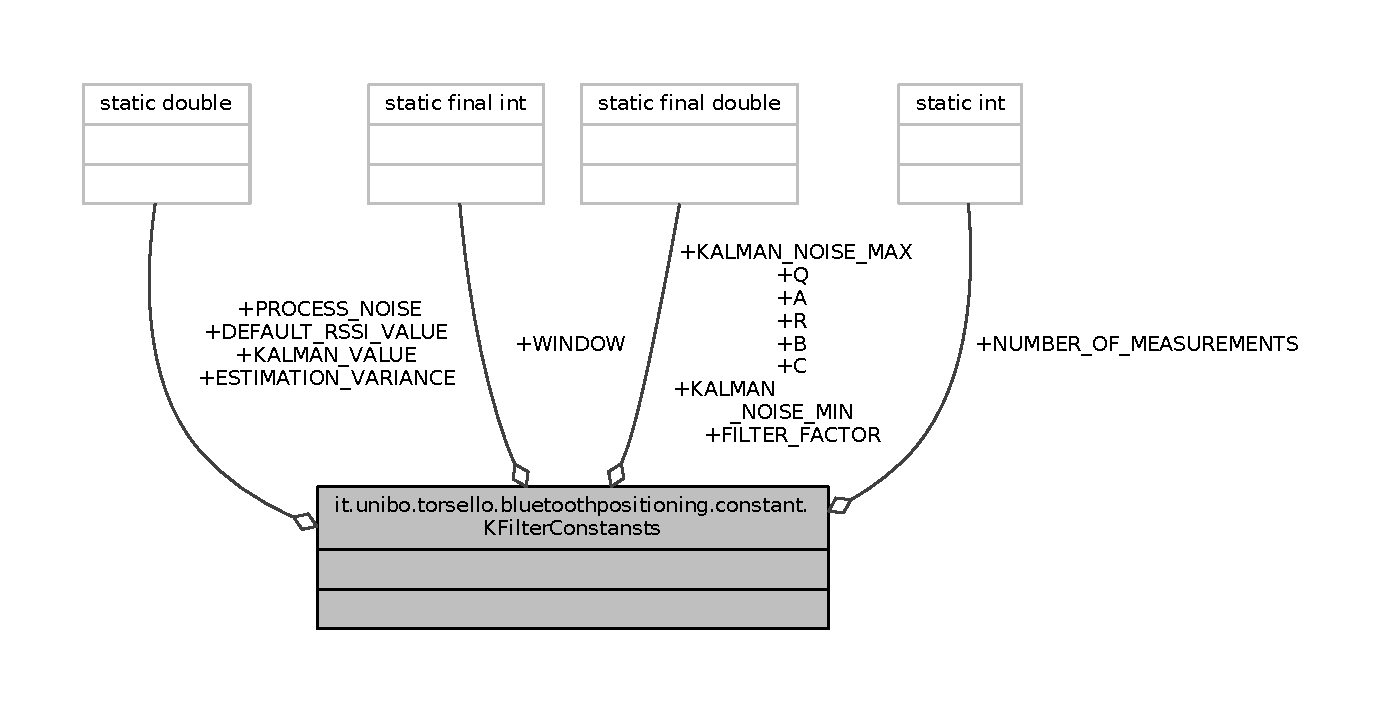
\includegraphics[width=350pt]{classit_1_1unibo_1_1torsello_1_1bluetoothpositioning_1_1constant_1_1KFilterConstansts__coll__graph}
\end{center}
\end{figure}
\subsubsection*{Attributi pubblici statici}
\begin{DoxyCompactItemize}
\item 
static final double \hyperlink{classit_1_1unibo_1_1torsello_1_1bluetoothpositioning_1_1constant_1_1KFilterConstansts_a5a45dca525813a3df9715cdf5878c289_a5a45dca525813a3df9715cdf5878c289}{K\+A\+L\+M\+A\+N\+\_\+\+N\+O\+I\+S\+E\+\_\+\+M\+IN} = 0.\+00D
\item 
static final double \hyperlink{classit_1_1unibo_1_1torsello_1_1bluetoothpositioning_1_1constant_1_1KFilterConstansts_af9b79f0b652105f894aa866ad8ae50f1_af9b79f0b652105f894aa866ad8ae50f1}{K\+A\+L\+M\+A\+N\+\_\+\+N\+O\+I\+S\+E\+\_\+\+M\+AX} = 5.\+0D
\item 
static final double \hyperlink{classit_1_1unibo_1_1torsello_1_1bluetoothpositioning_1_1constant_1_1KFilterConstansts_a9bc0f7f81fcbb7e9c18179df0d673e5b_a9bc0f7f81fcbb7e9c18179df0d673e5b}{F\+I\+L\+T\+E\+R\+\_\+\+F\+A\+C\+T\+OR} = 0.\+1D
\item 
static final int \hyperlink{classit_1_1unibo_1_1torsello_1_1bluetoothpositioning_1_1constant_1_1KFilterConstansts_aa33874174f7be9055504e154cb6b4baf_aa33874174f7be9055504e154cb6b4baf}{W\+I\+N\+D\+OW} = 20
\item 
static final double \hyperlink{classit_1_1unibo_1_1torsello_1_1bluetoothpositioning_1_1constant_1_1KFilterConstansts_aeebad8c471f2bcdf3328325cb548e429_aeebad8c471f2bcdf3328325cb548e429}{R} = 10
\item 
static final double \hyperlink{classit_1_1unibo_1_1torsello_1_1bluetoothpositioning_1_1constant_1_1KFilterConstansts_aa5bde73a61e5616d3217bdaf87fc6e78_aa5bde73a61e5616d3217bdaf87fc6e78}{Q} = 60.\+0
\item 
static final double \hyperlink{classit_1_1unibo_1_1torsello_1_1bluetoothpositioning_1_1constant_1_1KFilterConstansts_a6696f4c8bc06209b08dd308248b2b048_a6696f4c8bc06209b08dd308248b2b048}{A} = 1
\item 
static final double \hyperlink{classit_1_1unibo_1_1torsello_1_1bluetoothpositioning_1_1constant_1_1KFilterConstansts_a6fbe3fca27e3c7ef2df6aa9867685ff1_a6fbe3fca27e3c7ef2df6aa9867685ff1}{B} = 0
\item 
static final double \hyperlink{classit_1_1unibo_1_1torsello_1_1bluetoothpositioning_1_1constant_1_1KFilterConstansts_a4358950bbe93132edc3683ef9920a8a9_a4358950bbe93132edc3683ef9920a8a9}{C} = 1
\item 
static double \hyperlink{classit_1_1unibo_1_1torsello_1_1bluetoothpositioning_1_1constant_1_1KFilterConstansts_a6b01793427a35ab5da47686efeb87e92_a6b01793427a35ab5da47686efeb87e92}{K\+A\+L\+M\+A\+N\+\_\+\+V\+A\+L\+UE} = 2D
\item 
static double \hyperlink{classit_1_1unibo_1_1torsello_1_1bluetoothpositioning_1_1constant_1_1KFilterConstansts_a1f2a51a4c23f7cc42f602f641eaea368_a1f2a51a4c23f7cc42f602f641eaea368}{D\+E\+F\+A\+U\+L\+T\+\_\+\+R\+S\+S\+I\+\_\+\+V\+A\+L\+UE} = -\/70D
\item 
static int \hyperlink{classit_1_1unibo_1_1torsello_1_1bluetoothpositioning_1_1constant_1_1KFilterConstansts_a86eaaf60180d279244a49c4f0c874095_a86eaaf60180d279244a49c4f0c874095}{N\+U\+M\+B\+E\+R\+\_\+\+O\+F\+\_\+\+M\+E\+A\+S\+U\+R\+E\+M\+E\+N\+TS} = 1
\item 
static double \hyperlink{classit_1_1unibo_1_1torsello_1_1bluetoothpositioning_1_1constant_1_1KFilterConstansts_a286a9a856e4fe570d6d315039aa488cf_a286a9a856e4fe570d6d315039aa488cf}{E\+S\+T\+I\+M\+A\+T\+I\+O\+N\+\_\+\+V\+A\+R\+I\+A\+N\+CE} = 0.\+01D
\item 
static double \hyperlink{classit_1_1unibo_1_1torsello_1_1bluetoothpositioning_1_1constant_1_1KFilterConstansts_ab8b76f56fb1c22e0e48b01a31a5c8814_ab8b76f56fb1c22e0e48b01a31a5c8814}{P\+R\+O\+C\+E\+S\+S\+\_\+\+N\+O\+I\+SE} = 10
\end{DoxyCompactItemize}


\subsubsection{Descrizione dettagliata}
Created by Federico Torsello. \href{mailto:federico.torsello@studio.unibo.it}{\tt federico.\+torsello@studio.\+unibo.\+it} 

\subsubsection{Documentazione dei membri dato}
\hypertarget{classit_1_1unibo_1_1torsello_1_1bluetoothpositioning_1_1constant_1_1KFilterConstansts_a6696f4c8bc06209b08dd308248b2b048_a6696f4c8bc06209b08dd308248b2b048}{}\label{classit_1_1unibo_1_1torsello_1_1bluetoothpositioning_1_1constant_1_1KFilterConstansts_a6696f4c8bc06209b08dd308248b2b048_a6696f4c8bc06209b08dd308248b2b048} 
\index{it\+::unibo\+::torsello\+::bluetoothpositioning\+::constant\+::\+K\+Filter\+Constansts@{it\+::unibo\+::torsello\+::bluetoothpositioning\+::constant\+::\+K\+Filter\+Constansts}!A@{A}}
\index{A@{A}!it\+::unibo\+::torsello\+::bluetoothpositioning\+::constant\+::\+K\+Filter\+Constansts@{it\+::unibo\+::torsello\+::bluetoothpositioning\+::constant\+::\+K\+Filter\+Constansts}}
\paragraph{\texorpdfstring{A}{A}}
{\footnotesize\ttfamily final double it.\+unibo.\+torsello.\+bluetoothpositioning.\+constant.\+K\+Filter\+Constansts.\+A = 1\hspace{0.3cm}{\ttfamily [static]}}

\hypertarget{classit_1_1unibo_1_1torsello_1_1bluetoothpositioning_1_1constant_1_1KFilterConstansts_a6fbe3fca27e3c7ef2df6aa9867685ff1_a6fbe3fca27e3c7ef2df6aa9867685ff1}{}\label{classit_1_1unibo_1_1torsello_1_1bluetoothpositioning_1_1constant_1_1KFilterConstansts_a6fbe3fca27e3c7ef2df6aa9867685ff1_a6fbe3fca27e3c7ef2df6aa9867685ff1} 
\index{it\+::unibo\+::torsello\+::bluetoothpositioning\+::constant\+::\+K\+Filter\+Constansts@{it\+::unibo\+::torsello\+::bluetoothpositioning\+::constant\+::\+K\+Filter\+Constansts}!B@{B}}
\index{B@{B}!it\+::unibo\+::torsello\+::bluetoothpositioning\+::constant\+::\+K\+Filter\+Constansts@{it\+::unibo\+::torsello\+::bluetoothpositioning\+::constant\+::\+K\+Filter\+Constansts}}
\paragraph{\texorpdfstring{B}{B}}
{\footnotesize\ttfamily final double it.\+unibo.\+torsello.\+bluetoothpositioning.\+constant.\+K\+Filter\+Constansts.\+B = 0\hspace{0.3cm}{\ttfamily [static]}}

\hypertarget{classit_1_1unibo_1_1torsello_1_1bluetoothpositioning_1_1constant_1_1KFilterConstansts_a4358950bbe93132edc3683ef9920a8a9_a4358950bbe93132edc3683ef9920a8a9}{}\label{classit_1_1unibo_1_1torsello_1_1bluetoothpositioning_1_1constant_1_1KFilterConstansts_a4358950bbe93132edc3683ef9920a8a9_a4358950bbe93132edc3683ef9920a8a9} 
\index{it\+::unibo\+::torsello\+::bluetoothpositioning\+::constant\+::\+K\+Filter\+Constansts@{it\+::unibo\+::torsello\+::bluetoothpositioning\+::constant\+::\+K\+Filter\+Constansts}!C@{C}}
\index{C@{C}!it\+::unibo\+::torsello\+::bluetoothpositioning\+::constant\+::\+K\+Filter\+Constansts@{it\+::unibo\+::torsello\+::bluetoothpositioning\+::constant\+::\+K\+Filter\+Constansts}}
\paragraph{\texorpdfstring{C}{C}}
{\footnotesize\ttfamily final double it.\+unibo.\+torsello.\+bluetoothpositioning.\+constant.\+K\+Filter\+Constansts.\+C = 1\hspace{0.3cm}{\ttfamily [static]}}

\hypertarget{classit_1_1unibo_1_1torsello_1_1bluetoothpositioning_1_1constant_1_1KFilterConstansts_a1f2a51a4c23f7cc42f602f641eaea368_a1f2a51a4c23f7cc42f602f641eaea368}{}\label{classit_1_1unibo_1_1torsello_1_1bluetoothpositioning_1_1constant_1_1KFilterConstansts_a1f2a51a4c23f7cc42f602f641eaea368_a1f2a51a4c23f7cc42f602f641eaea368} 
\index{it\+::unibo\+::torsello\+::bluetoothpositioning\+::constant\+::\+K\+Filter\+Constansts@{it\+::unibo\+::torsello\+::bluetoothpositioning\+::constant\+::\+K\+Filter\+Constansts}!D\+E\+F\+A\+U\+L\+T\+\_\+\+R\+S\+S\+I\+\_\+\+V\+A\+L\+UE@{D\+E\+F\+A\+U\+L\+T\+\_\+\+R\+S\+S\+I\+\_\+\+V\+A\+L\+UE}}
\index{D\+E\+F\+A\+U\+L\+T\+\_\+\+R\+S\+S\+I\+\_\+\+V\+A\+L\+UE@{D\+E\+F\+A\+U\+L\+T\+\_\+\+R\+S\+S\+I\+\_\+\+V\+A\+L\+UE}!it\+::unibo\+::torsello\+::bluetoothpositioning\+::constant\+::\+K\+Filter\+Constansts@{it\+::unibo\+::torsello\+::bluetoothpositioning\+::constant\+::\+K\+Filter\+Constansts}}
\paragraph{\texorpdfstring{D\+E\+F\+A\+U\+L\+T\+\_\+\+R\+S\+S\+I\+\_\+\+V\+A\+L\+UE}{DEFAULT\_RSSI\_VALUE}}
{\footnotesize\ttfamily double it.\+unibo.\+torsello.\+bluetoothpositioning.\+constant.\+K\+Filter\+Constansts.\+D\+E\+F\+A\+U\+L\+T\+\_\+\+R\+S\+S\+I\+\_\+\+V\+A\+L\+UE = -\/70D\hspace{0.3cm}{\ttfamily [static]}}

\hypertarget{classit_1_1unibo_1_1torsello_1_1bluetoothpositioning_1_1constant_1_1KFilterConstansts_a286a9a856e4fe570d6d315039aa488cf_a286a9a856e4fe570d6d315039aa488cf}{}\label{classit_1_1unibo_1_1torsello_1_1bluetoothpositioning_1_1constant_1_1KFilterConstansts_a286a9a856e4fe570d6d315039aa488cf_a286a9a856e4fe570d6d315039aa488cf} 
\index{it\+::unibo\+::torsello\+::bluetoothpositioning\+::constant\+::\+K\+Filter\+Constansts@{it\+::unibo\+::torsello\+::bluetoothpositioning\+::constant\+::\+K\+Filter\+Constansts}!E\+S\+T\+I\+M\+A\+T\+I\+O\+N\+\_\+\+V\+A\+R\+I\+A\+N\+CE@{E\+S\+T\+I\+M\+A\+T\+I\+O\+N\+\_\+\+V\+A\+R\+I\+A\+N\+CE}}
\index{E\+S\+T\+I\+M\+A\+T\+I\+O\+N\+\_\+\+V\+A\+R\+I\+A\+N\+CE@{E\+S\+T\+I\+M\+A\+T\+I\+O\+N\+\_\+\+V\+A\+R\+I\+A\+N\+CE}!it\+::unibo\+::torsello\+::bluetoothpositioning\+::constant\+::\+K\+Filter\+Constansts@{it\+::unibo\+::torsello\+::bluetoothpositioning\+::constant\+::\+K\+Filter\+Constansts}}
\paragraph{\texorpdfstring{E\+S\+T\+I\+M\+A\+T\+I\+O\+N\+\_\+\+V\+A\+R\+I\+A\+N\+CE}{ESTIMATION\_VARIANCE}}
{\footnotesize\ttfamily double it.\+unibo.\+torsello.\+bluetoothpositioning.\+constant.\+K\+Filter\+Constansts.\+E\+S\+T\+I\+M\+A\+T\+I\+O\+N\+\_\+\+V\+A\+R\+I\+A\+N\+CE = 0.\+01D\hspace{0.3cm}{\ttfamily [static]}}

\hypertarget{classit_1_1unibo_1_1torsello_1_1bluetoothpositioning_1_1constant_1_1KFilterConstansts_a9bc0f7f81fcbb7e9c18179df0d673e5b_a9bc0f7f81fcbb7e9c18179df0d673e5b}{}\label{classit_1_1unibo_1_1torsello_1_1bluetoothpositioning_1_1constant_1_1KFilterConstansts_a9bc0f7f81fcbb7e9c18179df0d673e5b_a9bc0f7f81fcbb7e9c18179df0d673e5b} 
\index{it\+::unibo\+::torsello\+::bluetoothpositioning\+::constant\+::\+K\+Filter\+Constansts@{it\+::unibo\+::torsello\+::bluetoothpositioning\+::constant\+::\+K\+Filter\+Constansts}!F\+I\+L\+T\+E\+R\+\_\+\+F\+A\+C\+T\+OR@{F\+I\+L\+T\+E\+R\+\_\+\+F\+A\+C\+T\+OR}}
\index{F\+I\+L\+T\+E\+R\+\_\+\+F\+A\+C\+T\+OR@{F\+I\+L\+T\+E\+R\+\_\+\+F\+A\+C\+T\+OR}!it\+::unibo\+::torsello\+::bluetoothpositioning\+::constant\+::\+K\+Filter\+Constansts@{it\+::unibo\+::torsello\+::bluetoothpositioning\+::constant\+::\+K\+Filter\+Constansts}}
\paragraph{\texorpdfstring{F\+I\+L\+T\+E\+R\+\_\+\+F\+A\+C\+T\+OR}{FILTER\_FACTOR}}
{\footnotesize\ttfamily final double it.\+unibo.\+torsello.\+bluetoothpositioning.\+constant.\+K\+Filter\+Constansts.\+F\+I\+L\+T\+E\+R\+\_\+\+F\+A\+C\+T\+OR = 0.\+1D\hspace{0.3cm}{\ttfamily [static]}}

\hypertarget{classit_1_1unibo_1_1torsello_1_1bluetoothpositioning_1_1constant_1_1KFilterConstansts_af9b79f0b652105f894aa866ad8ae50f1_af9b79f0b652105f894aa866ad8ae50f1}{}\label{classit_1_1unibo_1_1torsello_1_1bluetoothpositioning_1_1constant_1_1KFilterConstansts_af9b79f0b652105f894aa866ad8ae50f1_af9b79f0b652105f894aa866ad8ae50f1} 
\index{it\+::unibo\+::torsello\+::bluetoothpositioning\+::constant\+::\+K\+Filter\+Constansts@{it\+::unibo\+::torsello\+::bluetoothpositioning\+::constant\+::\+K\+Filter\+Constansts}!K\+A\+L\+M\+A\+N\+\_\+\+N\+O\+I\+S\+E\+\_\+\+M\+AX@{K\+A\+L\+M\+A\+N\+\_\+\+N\+O\+I\+S\+E\+\_\+\+M\+AX}}
\index{K\+A\+L\+M\+A\+N\+\_\+\+N\+O\+I\+S\+E\+\_\+\+M\+AX@{K\+A\+L\+M\+A\+N\+\_\+\+N\+O\+I\+S\+E\+\_\+\+M\+AX}!it\+::unibo\+::torsello\+::bluetoothpositioning\+::constant\+::\+K\+Filter\+Constansts@{it\+::unibo\+::torsello\+::bluetoothpositioning\+::constant\+::\+K\+Filter\+Constansts}}
\paragraph{\texorpdfstring{K\+A\+L\+M\+A\+N\+\_\+\+N\+O\+I\+S\+E\+\_\+\+M\+AX}{KALMAN\_NOISE\_MAX}}
{\footnotesize\ttfamily final double it.\+unibo.\+torsello.\+bluetoothpositioning.\+constant.\+K\+Filter\+Constansts.\+K\+A\+L\+M\+A\+N\+\_\+\+N\+O\+I\+S\+E\+\_\+\+M\+AX = 5.\+0D\hspace{0.3cm}{\ttfamily [static]}}

\hypertarget{classit_1_1unibo_1_1torsello_1_1bluetoothpositioning_1_1constant_1_1KFilterConstansts_a5a45dca525813a3df9715cdf5878c289_a5a45dca525813a3df9715cdf5878c289}{}\label{classit_1_1unibo_1_1torsello_1_1bluetoothpositioning_1_1constant_1_1KFilterConstansts_a5a45dca525813a3df9715cdf5878c289_a5a45dca525813a3df9715cdf5878c289} 
\index{it\+::unibo\+::torsello\+::bluetoothpositioning\+::constant\+::\+K\+Filter\+Constansts@{it\+::unibo\+::torsello\+::bluetoothpositioning\+::constant\+::\+K\+Filter\+Constansts}!K\+A\+L\+M\+A\+N\+\_\+\+N\+O\+I\+S\+E\+\_\+\+M\+IN@{K\+A\+L\+M\+A\+N\+\_\+\+N\+O\+I\+S\+E\+\_\+\+M\+IN}}
\index{K\+A\+L\+M\+A\+N\+\_\+\+N\+O\+I\+S\+E\+\_\+\+M\+IN@{K\+A\+L\+M\+A\+N\+\_\+\+N\+O\+I\+S\+E\+\_\+\+M\+IN}!it\+::unibo\+::torsello\+::bluetoothpositioning\+::constant\+::\+K\+Filter\+Constansts@{it\+::unibo\+::torsello\+::bluetoothpositioning\+::constant\+::\+K\+Filter\+Constansts}}
\paragraph{\texorpdfstring{K\+A\+L\+M\+A\+N\+\_\+\+N\+O\+I\+S\+E\+\_\+\+M\+IN}{KALMAN\_NOISE\_MIN}}
{\footnotesize\ttfamily final double it.\+unibo.\+torsello.\+bluetoothpositioning.\+constant.\+K\+Filter\+Constansts.\+K\+A\+L\+M\+A\+N\+\_\+\+N\+O\+I\+S\+E\+\_\+\+M\+IN = 0.\+00D\hspace{0.3cm}{\ttfamily [static]}}

\hypertarget{classit_1_1unibo_1_1torsello_1_1bluetoothpositioning_1_1constant_1_1KFilterConstansts_a6b01793427a35ab5da47686efeb87e92_a6b01793427a35ab5da47686efeb87e92}{}\label{classit_1_1unibo_1_1torsello_1_1bluetoothpositioning_1_1constant_1_1KFilterConstansts_a6b01793427a35ab5da47686efeb87e92_a6b01793427a35ab5da47686efeb87e92} 
\index{it\+::unibo\+::torsello\+::bluetoothpositioning\+::constant\+::\+K\+Filter\+Constansts@{it\+::unibo\+::torsello\+::bluetoothpositioning\+::constant\+::\+K\+Filter\+Constansts}!K\+A\+L\+M\+A\+N\+\_\+\+V\+A\+L\+UE@{K\+A\+L\+M\+A\+N\+\_\+\+V\+A\+L\+UE}}
\index{K\+A\+L\+M\+A\+N\+\_\+\+V\+A\+L\+UE@{K\+A\+L\+M\+A\+N\+\_\+\+V\+A\+L\+UE}!it\+::unibo\+::torsello\+::bluetoothpositioning\+::constant\+::\+K\+Filter\+Constansts@{it\+::unibo\+::torsello\+::bluetoothpositioning\+::constant\+::\+K\+Filter\+Constansts}}
\paragraph{\texorpdfstring{K\+A\+L\+M\+A\+N\+\_\+\+V\+A\+L\+UE}{KALMAN\_VALUE}}
{\footnotesize\ttfamily double it.\+unibo.\+torsello.\+bluetoothpositioning.\+constant.\+K\+Filter\+Constansts.\+K\+A\+L\+M\+A\+N\+\_\+\+V\+A\+L\+UE = 2D\hspace{0.3cm}{\ttfamily [static]}}

\hypertarget{classit_1_1unibo_1_1torsello_1_1bluetoothpositioning_1_1constant_1_1KFilterConstansts_a86eaaf60180d279244a49c4f0c874095_a86eaaf60180d279244a49c4f0c874095}{}\label{classit_1_1unibo_1_1torsello_1_1bluetoothpositioning_1_1constant_1_1KFilterConstansts_a86eaaf60180d279244a49c4f0c874095_a86eaaf60180d279244a49c4f0c874095} 
\index{it\+::unibo\+::torsello\+::bluetoothpositioning\+::constant\+::\+K\+Filter\+Constansts@{it\+::unibo\+::torsello\+::bluetoothpositioning\+::constant\+::\+K\+Filter\+Constansts}!N\+U\+M\+B\+E\+R\+\_\+\+O\+F\+\_\+\+M\+E\+A\+S\+U\+R\+E\+M\+E\+N\+TS@{N\+U\+M\+B\+E\+R\+\_\+\+O\+F\+\_\+\+M\+E\+A\+S\+U\+R\+E\+M\+E\+N\+TS}}
\index{N\+U\+M\+B\+E\+R\+\_\+\+O\+F\+\_\+\+M\+E\+A\+S\+U\+R\+E\+M\+E\+N\+TS@{N\+U\+M\+B\+E\+R\+\_\+\+O\+F\+\_\+\+M\+E\+A\+S\+U\+R\+E\+M\+E\+N\+TS}!it\+::unibo\+::torsello\+::bluetoothpositioning\+::constant\+::\+K\+Filter\+Constansts@{it\+::unibo\+::torsello\+::bluetoothpositioning\+::constant\+::\+K\+Filter\+Constansts}}
\paragraph{\texorpdfstring{N\+U\+M\+B\+E\+R\+\_\+\+O\+F\+\_\+\+M\+E\+A\+S\+U\+R\+E\+M\+E\+N\+TS}{NUMBER\_OF\_MEASUREMENTS}}
{\footnotesize\ttfamily int it.\+unibo.\+torsello.\+bluetoothpositioning.\+constant.\+K\+Filter\+Constansts.\+N\+U\+M\+B\+E\+R\+\_\+\+O\+F\+\_\+\+M\+E\+A\+S\+U\+R\+E\+M\+E\+N\+TS = 1\hspace{0.3cm}{\ttfamily [static]}}

\hypertarget{classit_1_1unibo_1_1torsello_1_1bluetoothpositioning_1_1constant_1_1KFilterConstansts_ab8b76f56fb1c22e0e48b01a31a5c8814_ab8b76f56fb1c22e0e48b01a31a5c8814}{}\label{classit_1_1unibo_1_1torsello_1_1bluetoothpositioning_1_1constant_1_1KFilterConstansts_ab8b76f56fb1c22e0e48b01a31a5c8814_ab8b76f56fb1c22e0e48b01a31a5c8814} 
\index{it\+::unibo\+::torsello\+::bluetoothpositioning\+::constant\+::\+K\+Filter\+Constansts@{it\+::unibo\+::torsello\+::bluetoothpositioning\+::constant\+::\+K\+Filter\+Constansts}!P\+R\+O\+C\+E\+S\+S\+\_\+\+N\+O\+I\+SE@{P\+R\+O\+C\+E\+S\+S\+\_\+\+N\+O\+I\+SE}}
\index{P\+R\+O\+C\+E\+S\+S\+\_\+\+N\+O\+I\+SE@{P\+R\+O\+C\+E\+S\+S\+\_\+\+N\+O\+I\+SE}!it\+::unibo\+::torsello\+::bluetoothpositioning\+::constant\+::\+K\+Filter\+Constansts@{it\+::unibo\+::torsello\+::bluetoothpositioning\+::constant\+::\+K\+Filter\+Constansts}}
\paragraph{\texorpdfstring{P\+R\+O\+C\+E\+S\+S\+\_\+\+N\+O\+I\+SE}{PROCESS\_NOISE}}
{\footnotesize\ttfamily double it.\+unibo.\+torsello.\+bluetoothpositioning.\+constant.\+K\+Filter\+Constansts.\+P\+R\+O\+C\+E\+S\+S\+\_\+\+N\+O\+I\+SE = 10\hspace{0.3cm}{\ttfamily [static]}}

\hypertarget{classit_1_1unibo_1_1torsello_1_1bluetoothpositioning_1_1constant_1_1KFilterConstansts_aa5bde73a61e5616d3217bdaf87fc6e78_aa5bde73a61e5616d3217bdaf87fc6e78}{}\label{classit_1_1unibo_1_1torsello_1_1bluetoothpositioning_1_1constant_1_1KFilterConstansts_aa5bde73a61e5616d3217bdaf87fc6e78_aa5bde73a61e5616d3217bdaf87fc6e78} 
\index{it\+::unibo\+::torsello\+::bluetoothpositioning\+::constant\+::\+K\+Filter\+Constansts@{it\+::unibo\+::torsello\+::bluetoothpositioning\+::constant\+::\+K\+Filter\+Constansts}!Q@{Q}}
\index{Q@{Q}!it\+::unibo\+::torsello\+::bluetoothpositioning\+::constant\+::\+K\+Filter\+Constansts@{it\+::unibo\+::torsello\+::bluetoothpositioning\+::constant\+::\+K\+Filter\+Constansts}}
\paragraph{\texorpdfstring{Q}{Q}}
{\footnotesize\ttfamily final double it.\+unibo.\+torsello.\+bluetoothpositioning.\+constant.\+K\+Filter\+Constansts.\+Q = 60.\+0\hspace{0.3cm}{\ttfamily [static]}}

\hypertarget{classit_1_1unibo_1_1torsello_1_1bluetoothpositioning_1_1constant_1_1KFilterConstansts_aeebad8c471f2bcdf3328325cb548e429_aeebad8c471f2bcdf3328325cb548e429}{}\label{classit_1_1unibo_1_1torsello_1_1bluetoothpositioning_1_1constant_1_1KFilterConstansts_aeebad8c471f2bcdf3328325cb548e429_aeebad8c471f2bcdf3328325cb548e429} 
\index{it\+::unibo\+::torsello\+::bluetoothpositioning\+::constant\+::\+K\+Filter\+Constansts@{it\+::unibo\+::torsello\+::bluetoothpositioning\+::constant\+::\+K\+Filter\+Constansts}!R@{R}}
\index{R@{R}!it\+::unibo\+::torsello\+::bluetoothpositioning\+::constant\+::\+K\+Filter\+Constansts@{it\+::unibo\+::torsello\+::bluetoothpositioning\+::constant\+::\+K\+Filter\+Constansts}}
\paragraph{\texorpdfstring{R}{R}}
{\footnotesize\ttfamily final double it.\+unibo.\+torsello.\+bluetoothpositioning.\+constant.\+K\+Filter\+Constansts.\+R = 10\hspace{0.3cm}{\ttfamily [static]}}

\hypertarget{classit_1_1unibo_1_1torsello_1_1bluetoothpositioning_1_1constant_1_1KFilterConstansts_aa33874174f7be9055504e154cb6b4baf_aa33874174f7be9055504e154cb6b4baf}{}\label{classit_1_1unibo_1_1torsello_1_1bluetoothpositioning_1_1constant_1_1KFilterConstansts_aa33874174f7be9055504e154cb6b4baf_aa33874174f7be9055504e154cb6b4baf} 
\index{it\+::unibo\+::torsello\+::bluetoothpositioning\+::constant\+::\+K\+Filter\+Constansts@{it\+::unibo\+::torsello\+::bluetoothpositioning\+::constant\+::\+K\+Filter\+Constansts}!W\+I\+N\+D\+OW@{W\+I\+N\+D\+OW}}
\index{W\+I\+N\+D\+OW@{W\+I\+N\+D\+OW}!it\+::unibo\+::torsello\+::bluetoothpositioning\+::constant\+::\+K\+Filter\+Constansts@{it\+::unibo\+::torsello\+::bluetoothpositioning\+::constant\+::\+K\+Filter\+Constansts}}
\paragraph{\texorpdfstring{W\+I\+N\+D\+OW}{WINDOW}}
{\footnotesize\ttfamily final int it.\+unibo.\+torsello.\+bluetoothpositioning.\+constant.\+K\+Filter\+Constansts.\+W\+I\+N\+D\+OW = 20\hspace{0.3cm}{\ttfamily [static]}}



La documentazione per questa classe è stata generata a partire dal seguente file\+:\begin{DoxyCompactItemize}
\item 
\hyperlink{KFilterConstansts_8java}{K\+Filter\+Constansts.\+java}\end{DoxyCompactItemize}

\hypertarget{classit_1_1unibo_1_1torsello_1_1bluetoothpositioning_1_1activities_1_1MainActivity}{}\subsection{Riferimenti per la classe it.\+unibo.\+torsello.\+bluetoothpositioning.\+activities.\+Main\+Activity}
\label{classit_1_1unibo_1_1torsello_1_1bluetoothpositioning_1_1activities_1_1MainActivity}\index{it.\+unibo.\+torsello.\+bluetoothpositioning.\+activities.\+Main\+Activity@{it.\+unibo.\+torsello.\+bluetoothpositioning.\+activities.\+Main\+Activity}}


Diagramma delle classi per it.\+unibo.\+torsello.\+bluetoothpositioning.\+activities.\+Main\+Activity
\nopagebreak
\begin{figure}[H]
\begin{center}
\leavevmode
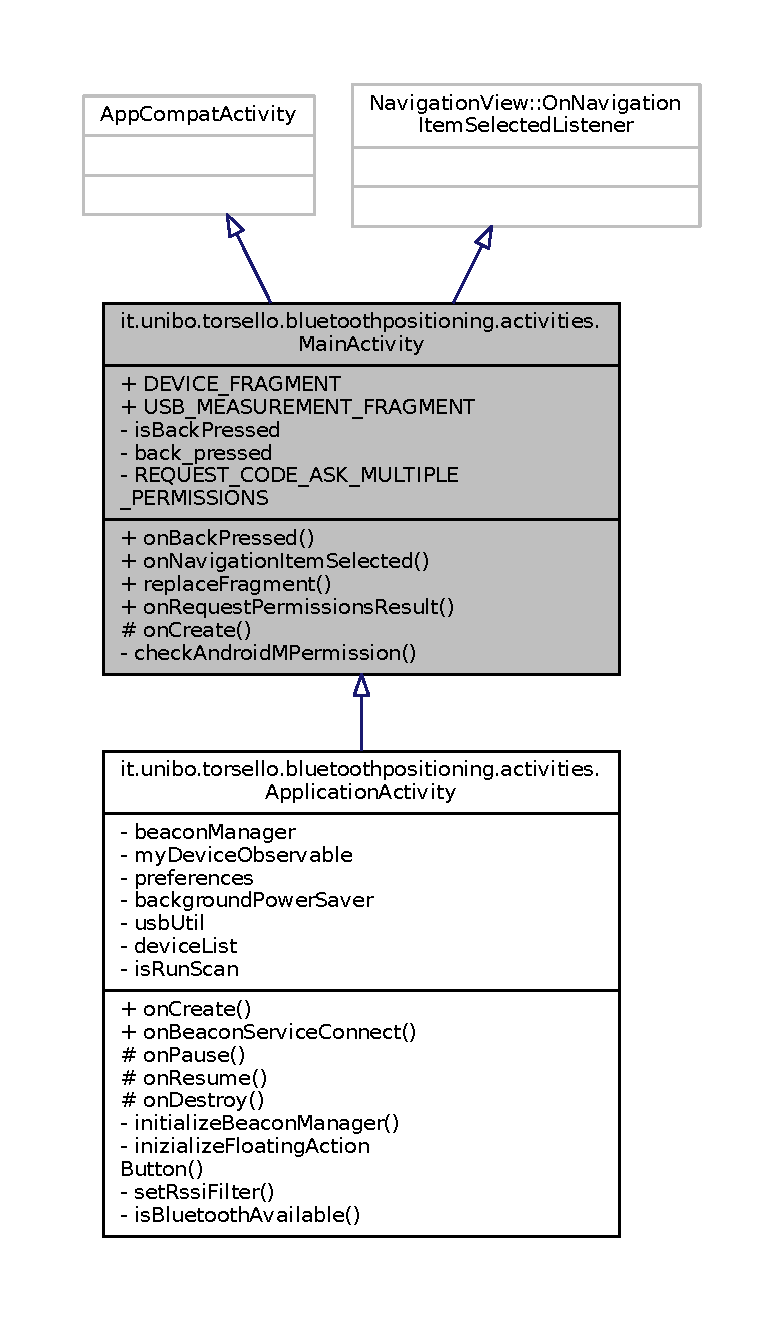
\includegraphics[height=550pt]{classit_1_1unibo_1_1torsello_1_1bluetoothpositioning_1_1activities_1_1MainActivity__inherit__graph}
\end{center}
\end{figure}


Diagramma di collaborazione per it.\+unibo.\+torsello.\+bluetoothpositioning.\+activities.\+Main\+Activity\+:
\nopagebreak
\begin{figure}[H]
\begin{center}
\leavevmode
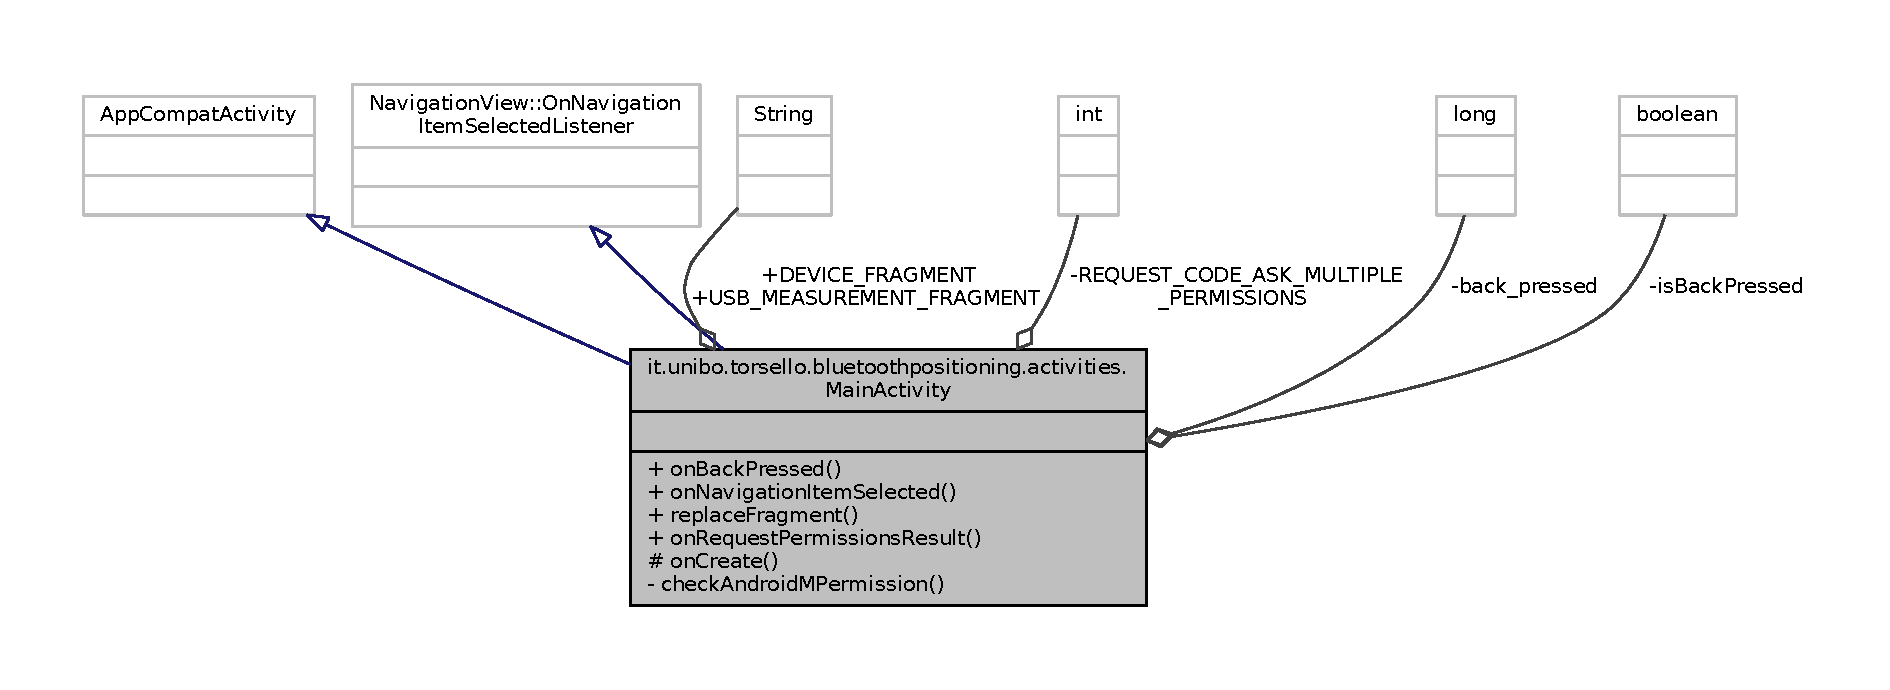
\includegraphics[width=350pt]{classit_1_1unibo_1_1torsello_1_1bluetoothpositioning_1_1activities_1_1MainActivity__coll__graph}
\end{center}
\end{figure}
\subsubsection*{Membri pubblici}
\begin{DoxyCompactItemize}
\item 
void \hyperlink{classit_1_1unibo_1_1torsello_1_1bluetoothpositioning_1_1activities_1_1MainActivity_ab0010b6d3fe518fabfea843626d7b5f1_ab0010b6d3fe518fabfea843626d7b5f1}{on\+Back\+Pressed} ()
\item 
boolean \hyperlink{classit_1_1unibo_1_1torsello_1_1bluetoothpositioning_1_1activities_1_1MainActivity_a7cfc0a2ee94c12afaac3b7472eeb75b7_a7cfc0a2ee94c12afaac3b7472eeb75b7}{on\+Navigation\+Item\+Selected} (Menu\+Item item)
\item 
void \hyperlink{classit_1_1unibo_1_1torsello_1_1bluetoothpositioning_1_1activities_1_1MainActivity_a98db4478d28cd91118138d0b652ceb2c_a98db4478d28cd91118138d0b652ceb2c}{replace\+Fragment} (String frag\+Tag)
\item 
void \hyperlink{classit_1_1unibo_1_1torsello_1_1bluetoothpositioning_1_1activities_1_1MainActivity_a81d7581dfa4998b2ad8139f103328cf9_a81d7581dfa4998b2ad8139f103328cf9}{on\+Request\+Permissions\+Result} (int request\+Code, @Non\+Null String permissions\mbox{[}$\,$\mbox{]}, @Non\+Null int\mbox{[}$\,$\mbox{]} grant\+Results)
\end{DoxyCompactItemize}
\subsubsection*{Attributi pubblici statici}
\begin{DoxyCompactItemize}
\item 
static final String \hyperlink{classit_1_1unibo_1_1torsello_1_1bluetoothpositioning_1_1activities_1_1MainActivity_a2f77c0245ac2525dc58905e38e1817d1_a2f77c0245ac2525dc58905e38e1817d1}{D\+E\+V\+I\+C\+E\+\_\+\+F\+R\+A\+G\+M\+E\+NT} = \char`\"{}device\char`\"{}
\item 
static final String \hyperlink{classit_1_1unibo_1_1torsello_1_1bluetoothpositioning_1_1activities_1_1MainActivity_a64bac06e6db556ba1e36c8773e61137b_a64bac06e6db556ba1e36c8773e61137b}{U\+S\+B\+\_\+\+M\+E\+A\+S\+U\+R\+E\+M\+E\+N\+T\+\_\+\+F\+R\+A\+G\+M\+E\+NT} = \char`\"{}usb measurement\char`\"{}
\end{DoxyCompactItemize}
\subsubsection*{Membri protetti}
\begin{DoxyCompactItemize}
\item 
void \hyperlink{classit_1_1unibo_1_1torsello_1_1bluetoothpositioning_1_1activities_1_1MainActivity_a8ffa5fa91fb4ae13a758a12682872a79_a8ffa5fa91fb4ae13a758a12682872a79}{on\+Create} (Bundle saved\+Instance\+State)
\end{DoxyCompactItemize}
\subsubsection*{Membri privati}
\begin{DoxyCompactItemize}
\item 
void \hyperlink{classit_1_1unibo_1_1torsello_1_1bluetoothpositioning_1_1activities_1_1MainActivity_ab762aac3d11f5b0ccc6042a140804d5d_ab762aac3d11f5b0ccc6042a140804d5d}{check\+Android\+M\+Permission} ()
\end{DoxyCompactItemize}
\subsubsection*{Attributi privati}
\begin{DoxyCompactItemize}
\item 
final String \hyperlink{classit_1_1unibo_1_1torsello_1_1bluetoothpositioning_1_1activities_1_1MainActivity_ab45ec7669a9285270b5dc817334762b3_ab45ec7669a9285270b5dc817334762b3}{T\+A\+G\+\_\+\+C\+L\+A\+SS} = get\+Class().get\+Simple\+Name()
\item 
boolean \hyperlink{classit_1_1unibo_1_1torsello_1_1bluetoothpositioning_1_1activities_1_1MainActivity_a73d74411ec7bb55eb827bb81018174bd_a73d74411ec7bb55eb827bb81018174bd}{is\+Back\+Pressed} = false
\item 
long \hyperlink{classit_1_1unibo_1_1torsello_1_1bluetoothpositioning_1_1activities_1_1MainActivity_a5e1ae38b2bbdcc45f2164fdc393ca495_a5e1ae38b2bbdcc45f2164fdc393ca495}{back\+\_\+pressed}
\item 
final int \hyperlink{classit_1_1unibo_1_1torsello_1_1bluetoothpositioning_1_1activities_1_1MainActivity_a319aed5cdd5724e043302babe5fcfeac_a319aed5cdd5724e043302babe5fcfeac}{R\+E\+Q\+U\+E\+S\+T\+\_\+\+C\+O\+D\+E\+\_\+\+A\+S\+K\+\_\+\+M\+U\+L\+T\+I\+P\+L\+E\+\_\+\+P\+E\+R\+M\+I\+S\+S\+I\+O\+NS} = 124
\end{DoxyCompactItemize}


\subsubsection{Descrizione dettagliata}
Created by Federico Torsello. \href{mailto:federico.torsello@studio.unibo.it}{\tt federico.\+torsello@studio.\+unibo.\+it} 

\subsubsection{Documentazione delle funzioni membro}
\hypertarget{classit_1_1unibo_1_1torsello_1_1bluetoothpositioning_1_1activities_1_1MainActivity_ab762aac3d11f5b0ccc6042a140804d5d_ab762aac3d11f5b0ccc6042a140804d5d}{}\label{classit_1_1unibo_1_1torsello_1_1bluetoothpositioning_1_1activities_1_1MainActivity_ab762aac3d11f5b0ccc6042a140804d5d_ab762aac3d11f5b0ccc6042a140804d5d} 
\index{it\+::unibo\+::torsello\+::bluetoothpositioning\+::activities\+::\+Main\+Activity@{it\+::unibo\+::torsello\+::bluetoothpositioning\+::activities\+::\+Main\+Activity}!check\+Android\+M\+Permission@{check\+Android\+M\+Permission}}
\index{check\+Android\+M\+Permission@{check\+Android\+M\+Permission}!it\+::unibo\+::torsello\+::bluetoothpositioning\+::activities\+::\+Main\+Activity@{it\+::unibo\+::torsello\+::bluetoothpositioning\+::activities\+::\+Main\+Activity}}
\paragraph{\texorpdfstring{check\+Android\+M\+Permission()}{checkAndroidMPermission()}}
{\footnotesize\ttfamily void it.\+unibo.\+torsello.\+bluetoothpositioning.\+activities.\+Main\+Activity.\+check\+Android\+M\+Permission (\begin{DoxyParamCaption}{ }\end{DoxyParamCaption})\hspace{0.3cm}{\ttfamily [private]}}


\begin{DoxyCode}
173                                            \{
174 
175         \textcolor{keywordflow}{if} (Build.VERSION.SDK\_INT >= Build.VERSION\_CODES.M) \{
176             \textcolor{keyword}{final} List<String> permissions = \textcolor{keyword}{new} ArrayList<>();
177 
178             \textcolor{keywordflow}{if} (checkSelfPermission(Manifest.permission.ACCESS\_FINE\_LOCATION)
179                     != PackageManager.PERMISSION\_GRANTED) \{
180                 permissions.add(Manifest.permission.ACCESS\_FINE\_LOCATION);
181             \}
182 
183             \textcolor{keywordflow}{if} (checkSelfPermission(Manifest.permission.ACCESS\_COARSE\_LOCATION)
184                     != PackageManager.PERMISSION\_GRANTED) \{
185                 permissions.add(Manifest.permission.ACCESS\_COARSE\_LOCATION);
186             \}
187 
188             \textcolor{keywordflow}{if} (!permissions.isEmpty()) \{
189                 \textcolor{keyword}{new} AlertDialog.Builder(\textcolor{keyword}{this})
190                         .setTitle(R.string.dialog\_location\_access\_title)
191                         .setMessage(R.string.dialog\_bluetooth\_text)
192                         .setPositiveButton(android.R.string.ok, null)
193                         .setOnDismissListener(\textcolor{keyword}{new} DialogInterface.OnDismissListener() \{
194                             @TargetApi(23)
195                             @Override
196                             \textcolor{keyword}{public} \textcolor{keywordtype}{void} onDismiss(DialogInterface dialog) \{
197                                 requestPermissions(permissions.toArray(\textcolor{keyword}{new} String[permissions.size()]),
198                                         \hyperlink{classit_1_1unibo_1_1torsello_1_1bluetoothpositioning_1_1activities_1_1MainActivity_a319aed5cdd5724e043302babe5fcfeac_a319aed5cdd5724e043302babe5fcfeac}{REQUEST\_CODE\_ASK\_MULTIPLE\_PERMISSIONS}
      );
199                             \}
200 
201                         \}).show();
202             \}
203         \}
204     \}
\end{DoxyCode}
\hypertarget{classit_1_1unibo_1_1torsello_1_1bluetoothpositioning_1_1activities_1_1MainActivity_ab0010b6d3fe518fabfea843626d7b5f1_ab0010b6d3fe518fabfea843626d7b5f1}{}\label{classit_1_1unibo_1_1torsello_1_1bluetoothpositioning_1_1activities_1_1MainActivity_ab0010b6d3fe518fabfea843626d7b5f1_ab0010b6d3fe518fabfea843626d7b5f1} 
\index{it\+::unibo\+::torsello\+::bluetoothpositioning\+::activities\+::\+Main\+Activity@{it\+::unibo\+::torsello\+::bluetoothpositioning\+::activities\+::\+Main\+Activity}!on\+Back\+Pressed@{on\+Back\+Pressed}}
\index{on\+Back\+Pressed@{on\+Back\+Pressed}!it\+::unibo\+::torsello\+::bluetoothpositioning\+::activities\+::\+Main\+Activity@{it\+::unibo\+::torsello\+::bluetoothpositioning\+::activities\+::\+Main\+Activity}}
\paragraph{\texorpdfstring{on\+Back\+Pressed()}{onBackPressed()}}
{\footnotesize\ttfamily void it.\+unibo.\+torsello.\+bluetoothpositioning.\+activities.\+Main\+Activity.\+on\+Back\+Pressed (\begin{DoxyParamCaption}{ }\end{DoxyParamCaption})}


\begin{DoxyCode}
70                                 \{
71 
72         DrawerLayout drawer = (DrawerLayout) findViewById(R.id.drawer\_layout);
73         \textcolor{keywordflow}{if} (drawer.isDrawerOpen(GravityCompat.START)) \{
74             drawer.closeDrawer(GravityCompat.START);
75         \} \textcolor{keywordflow}{else} \textcolor{keywordflow}{if} (drawer.isDrawerOpen(GravityCompat.END)) \{
76             drawer.closeDrawer(GravityCompat.END);
77         \} \textcolor{keywordflow}{else} \{
78 
79             \hyperlink{classit_1_1unibo_1_1torsello_1_1bluetoothpositioning_1_1activities_1_1MainActivity_a98db4478d28cd91118138d0b652ceb2c_a98db4478d28cd91118138d0b652ceb2c}{replaceFragment}(\hyperlink{classit_1_1unibo_1_1torsello_1_1bluetoothpositioning_1_1activities_1_1MainActivity_a2f77c0245ac2525dc58905e38e1817d1_a2f77c0245ac2525dc58905e38e1817d1}{DEVICE\_FRAGMENT});
80 
81             \textcolor{keyword}{final} \textcolor{keywordtype}{long} DOUBLE\_PRESS\_INTERVAL = 1500L;
82             \textcolor{keywordflow}{if} (!\hyperlink{classit_1_1unibo_1_1torsello_1_1bluetoothpositioning_1_1activities_1_1MainActivity_a73d74411ec7bb55eb827bb81018174bd_a73d74411ec7bb55eb827bb81018174bd}{isBackPressed} || \hyperlink{classit_1_1unibo_1_1torsello_1_1bluetoothpositioning_1_1activities_1_1MainActivity_a5e1ae38b2bbdcc45f2164fdc393ca495_a5e1ae38b2bbdcc45f2164fdc393ca495}{back\_pressed} + DOUBLE\_PRESS\_INTERVAL <= System.
      currentTimeMillis()) \{
83                 \hyperlink{classit_1_1unibo_1_1torsello_1_1bluetoothpositioning_1_1activities_1_1MainActivity_a73d74411ec7bb55eb827bb81018174bd_a73d74411ec7bb55eb827bb81018174bd}{isBackPressed} = \textcolor{keyword}{true};
84                 FloatingActionButton fab = (FloatingActionButton) findViewById(R.id.fab);
85                 assert fab != null;
86                 Snackbar.make(fab, R.string.snackBar\_exit, Snackbar.LENGTH\_SHORT).show();
87             \} \textcolor{keywordflow}{else} \{
88                 super.finish();
89             \}
90             \hyperlink{classit_1_1unibo_1_1torsello_1_1bluetoothpositioning_1_1activities_1_1MainActivity_a5e1ae38b2bbdcc45f2164fdc393ca495_a5e1ae38b2bbdcc45f2164fdc393ca495}{back\_pressed} = System.currentTimeMillis();
91         \}
92     \}
\end{DoxyCode}
\hypertarget{classit_1_1unibo_1_1torsello_1_1bluetoothpositioning_1_1activities_1_1MainActivity_a8ffa5fa91fb4ae13a758a12682872a79_a8ffa5fa91fb4ae13a758a12682872a79}{}\label{classit_1_1unibo_1_1torsello_1_1bluetoothpositioning_1_1activities_1_1MainActivity_a8ffa5fa91fb4ae13a758a12682872a79_a8ffa5fa91fb4ae13a758a12682872a79} 
\index{it\+::unibo\+::torsello\+::bluetoothpositioning\+::activities\+::\+Main\+Activity@{it\+::unibo\+::torsello\+::bluetoothpositioning\+::activities\+::\+Main\+Activity}!on\+Create@{on\+Create}}
\index{on\+Create@{on\+Create}!it\+::unibo\+::torsello\+::bluetoothpositioning\+::activities\+::\+Main\+Activity@{it\+::unibo\+::torsello\+::bluetoothpositioning\+::activities\+::\+Main\+Activity}}
\paragraph{\texorpdfstring{on\+Create()}{onCreate()}}
{\footnotesize\ttfamily void it.\+unibo.\+torsello.\+bluetoothpositioning.\+activities.\+Main\+Activity.\+on\+Create (\begin{DoxyParamCaption}\item[{Bundle}]{saved\+Instance\+State }\end{DoxyParamCaption})\hspace{0.3cm}{\ttfamily [protected]}}


\begin{DoxyCode}
47                                                        \{
48         super.onCreate(savedInstanceState);
49         setContentView(R.layout.activity\_main);
50 
51         Toolbar toolbar = (Toolbar) findViewById(R.id.toolbar);
52         setSupportActionBar(toolbar);
53 
54         DrawerLayout drawer = (DrawerLayout) findViewById(R.id.drawer\_layout);
55         ActionBarDrawerToggle toggle = \textcolor{keyword}{new} ActionBarDrawerToggle(
56                 \textcolor{keyword}{this}, drawer, toolbar, R.string.navigation\_drawer\_open, R.string.navigation\_drawer\_close);
57         drawer.addDrawerListener(toggle);
58         toggle.syncState();
59 
60         ((NavigationView) findViewById(R.id.nav\_view)).setNavigationItemSelectedListener(\textcolor{keyword}{this});
61 
62         ((NavigationView) findViewById(R.id.nav\_view2)).setNavigationItemSelectedListener(\textcolor{keyword}{this});
63 
64         \hyperlink{classit_1_1unibo_1_1torsello_1_1bluetoothpositioning_1_1activities_1_1MainActivity_a98db4478d28cd91118138d0b652ceb2c_a98db4478d28cd91118138d0b652ceb2c}{replaceFragment}(\hyperlink{classit_1_1unibo_1_1torsello_1_1bluetoothpositioning_1_1activities_1_1MainActivity_a2f77c0245ac2525dc58905e38e1817d1_a2f77c0245ac2525dc58905e38e1817d1}{DEVICE\_FRAGMENT});
65 
66         \hyperlink{classit_1_1unibo_1_1torsello_1_1bluetoothpositioning_1_1activities_1_1MainActivity_ab762aac3d11f5b0ccc6042a140804d5d_ab762aac3d11f5b0ccc6042a140804d5d}{checkAndroidMPermission}();
67     \}
\end{DoxyCode}
\hypertarget{classit_1_1unibo_1_1torsello_1_1bluetoothpositioning_1_1activities_1_1MainActivity_a7cfc0a2ee94c12afaac3b7472eeb75b7_a7cfc0a2ee94c12afaac3b7472eeb75b7}{}\label{classit_1_1unibo_1_1torsello_1_1bluetoothpositioning_1_1activities_1_1MainActivity_a7cfc0a2ee94c12afaac3b7472eeb75b7_a7cfc0a2ee94c12afaac3b7472eeb75b7} 
\index{it\+::unibo\+::torsello\+::bluetoothpositioning\+::activities\+::\+Main\+Activity@{it\+::unibo\+::torsello\+::bluetoothpositioning\+::activities\+::\+Main\+Activity}!on\+Navigation\+Item\+Selected@{on\+Navigation\+Item\+Selected}}
\index{on\+Navigation\+Item\+Selected@{on\+Navigation\+Item\+Selected}!it\+::unibo\+::torsello\+::bluetoothpositioning\+::activities\+::\+Main\+Activity@{it\+::unibo\+::torsello\+::bluetoothpositioning\+::activities\+::\+Main\+Activity}}
\paragraph{\texorpdfstring{on\+Navigation\+Item\+Selected()}{onNavigationItemSelected()}}
{\footnotesize\ttfamily boolean it.\+unibo.\+torsello.\+bluetoothpositioning.\+activities.\+Main\+Activity.\+on\+Navigation\+Item\+Selected (\begin{DoxyParamCaption}\item[{Menu\+Item}]{item }\end{DoxyParamCaption})}


\begin{DoxyCode}
96                                                            \{
97 
98         DrawerLayout drawer = (DrawerLayout) findViewById(R.id.drawer\_layout);
99 
100         \textcolor{comment}{// Handle navigation view item clicks here.}
101         \textcolor{keywordflow}{switch} (item.getItemId()) \{
102             \textcolor{keywordflow}{case} R.id.nav\_home:
103                 \hyperlink{classit_1_1unibo_1_1torsello_1_1bluetoothpositioning_1_1activities_1_1MainActivity_a98db4478d28cd91118138d0b652ceb2c_a98db4478d28cd91118138d0b652ceb2c}{replaceFragment}(\hyperlink{classit_1_1unibo_1_1torsello_1_1bluetoothpositioning_1_1activities_1_1MainActivity_a2f77c0245ac2525dc58905e38e1817d1_a2f77c0245ac2525dc58905e38e1817d1}{DEVICE\_FRAGMENT});
104                 \textcolor{keywordflow}{break};
105             \textcolor{keywordflow}{case} R.id.nav\_settings:
106                 drawer.openDrawer(GravityCompat.END);
107                 \textcolor{keywordflow}{break};
108             \textcolor{keywordflow}{case} R.id.nav\_measurement:
109                 \hyperlink{classit_1_1unibo_1_1torsello_1_1bluetoothpositioning_1_1activities_1_1MainActivity_a98db4478d28cd91118138d0b652ceb2c_a98db4478d28cd91118138d0b652ceb2c}{replaceFragment}(\hyperlink{classit_1_1unibo_1_1torsello_1_1bluetoothpositioning_1_1activities_1_1MainActivity_a64bac06e6db556ba1e36c8773e61137b_a64bac06e6db556ba1e36c8773e61137b}{USB\_MEASUREMENT\_FRAGMENT});
110                 \textcolor{keywordflow}{break};
111 \textcolor{comment}{//            case R.id.nav\_share:}
112 \textcolor{comment}{//                fragment = CamTestFragment.newInstance();}
113 \textcolor{comment}{//                break;}
114 \textcolor{comment}{//            case R.id.nav\_send:}
115 \textcolor{comment}{//                fragment = ViewPagerFragment.newInstance(getFragments());}
116 \textcolor{comment}{//                break;}
117         \}
118 
119         \textcolor{keywordflow}{if} (drawer.isDrawerOpen(GravityCompat.START)) \{
120             drawer.closeDrawer(GravityCompat.START);
121         \}
122 
123         \textcolor{keywordflow}{return} \textcolor{keyword}{true};
124     \}
\end{DoxyCode}
\hypertarget{classit_1_1unibo_1_1torsello_1_1bluetoothpositioning_1_1activities_1_1MainActivity_a81d7581dfa4998b2ad8139f103328cf9_a81d7581dfa4998b2ad8139f103328cf9}{}\label{classit_1_1unibo_1_1torsello_1_1bluetoothpositioning_1_1activities_1_1MainActivity_a81d7581dfa4998b2ad8139f103328cf9_a81d7581dfa4998b2ad8139f103328cf9} 
\index{it\+::unibo\+::torsello\+::bluetoothpositioning\+::activities\+::\+Main\+Activity@{it\+::unibo\+::torsello\+::bluetoothpositioning\+::activities\+::\+Main\+Activity}!on\+Request\+Permissions\+Result@{on\+Request\+Permissions\+Result}}
\index{on\+Request\+Permissions\+Result@{on\+Request\+Permissions\+Result}!it\+::unibo\+::torsello\+::bluetoothpositioning\+::activities\+::\+Main\+Activity@{it\+::unibo\+::torsello\+::bluetoothpositioning\+::activities\+::\+Main\+Activity}}
\paragraph{\texorpdfstring{on\+Request\+Permissions\+Result()}{onRequestPermissionsResult()}}
{\footnotesize\ttfamily void it.\+unibo.\+torsello.\+bluetoothpositioning.\+activities.\+Main\+Activity.\+on\+Request\+Permissions\+Result (\begin{DoxyParamCaption}\item[{int}]{request\+Code,  }\item[{@Non\+Null String}]{permissions\mbox{[}$\,$\mbox{]},  }\item[{@Non\+Null int \mbox{[}$\,$\mbox{]}}]{grant\+Results }\end{DoxyParamCaption})}


\begin{DoxyCode}
146                                                                         \{
147         \textcolor{keywordflow}{switch} (requestCode) \{
148             \textcolor{keywordflow}{case} \hyperlink{classit_1_1unibo_1_1torsello_1_1bluetoothpositioning_1_1activities_1_1MainActivity_a319aed5cdd5724e043302babe5fcfeac_a319aed5cdd5724e043302babe5fcfeac}{REQUEST\_CODE\_ASK\_MULTIPLE\_PERMISSIONS}:
149                 \textcolor{keywordflow}{for} (\textcolor{keywordtype}{int} i = 0; i < permissions.length; i++) \{
150                     \textcolor{keywordflow}{if} (grantResults[i] == PackageManager.PERMISSION\_GRANTED) \{
151 \textcolor{comment}{//                        Log.d(TAG\_CLASS, "Permission Granted: " + permissions[i]);}
152                     \} \textcolor{keywordflow}{else} \textcolor{keywordflow}{if} (grantResults[i] == PackageManager.PERMISSION\_DENIED) \{
153 \textcolor{comment}{//                        Log.d(TAG\_CLASS, "Permission Denied: " + permissions[i]);}
154                         \textcolor{keyword}{new} AlertDialog.Builder(\textcolor{keyword}{this})
155                                 .setTitle(R.string.dialog\_permissions\_location\_access\_title)
156                                 .setMessage(R.string.dialog\_permissions\_location\_access\_text)
157                                 .setPositiveButton(android.R.string.ok, null)
158                                 .setOnDismissListener(\textcolor{keyword}{new} DialogInterface.OnDismissListener() \{
159 
160                                     @Override
161                                     \textcolor{keyword}{public} \textcolor{keywordtype}{void} onDismiss(DialogInterface dialog) \{
162                                     \}
163 
164                                 \}).show();
165                     \}
166                 \}
167                 \textcolor{keywordflow}{break};
168             \textcolor{keywordflow}{default}:
169                 super.onRequestPermissionsResult(requestCode, permissions, grantResults);
170         \}
171     \}
\end{DoxyCode}
\hypertarget{classit_1_1unibo_1_1torsello_1_1bluetoothpositioning_1_1activities_1_1MainActivity_a98db4478d28cd91118138d0b652ceb2c_a98db4478d28cd91118138d0b652ceb2c}{}\label{classit_1_1unibo_1_1torsello_1_1bluetoothpositioning_1_1activities_1_1MainActivity_a98db4478d28cd91118138d0b652ceb2c_a98db4478d28cd91118138d0b652ceb2c} 
\index{it\+::unibo\+::torsello\+::bluetoothpositioning\+::activities\+::\+Main\+Activity@{it\+::unibo\+::torsello\+::bluetoothpositioning\+::activities\+::\+Main\+Activity}!replace\+Fragment@{replace\+Fragment}}
\index{replace\+Fragment@{replace\+Fragment}!it\+::unibo\+::torsello\+::bluetoothpositioning\+::activities\+::\+Main\+Activity@{it\+::unibo\+::torsello\+::bluetoothpositioning\+::activities\+::\+Main\+Activity}}
\paragraph{\texorpdfstring{replace\+Fragment()}{replaceFragment()}}
{\footnotesize\ttfamily void it.\+unibo.\+torsello.\+bluetoothpositioning.\+activities.\+Main\+Activity.\+replace\+Fragment (\begin{DoxyParamCaption}\item[{String}]{frag\+Tag }\end{DoxyParamCaption})}


\begin{DoxyCode}
126                                                 \{
127         Fragment currentFragment = getSupportFragmentManager().findFragmentByTag(fragTag);
128         \textcolor{keywordflow}{switch} (fragTag) \{
129             \textcolor{keywordflow}{case} \hyperlink{classit_1_1unibo_1_1torsello_1_1bluetoothpositioning_1_1activities_1_1MainActivity_a2f77c0245ac2525dc58905e38e1817d1_a2f77c0245ac2525dc58905e38e1817d1}{DEVICE\_FRAGMENT}:
130                 currentFragment = DeviceListFragment.newInstance();
131                 \textcolor{keywordflow}{break};
132             \textcolor{keywordflow}{case} \hyperlink{classit_1_1unibo_1_1torsello_1_1bluetoothpositioning_1_1activities_1_1MainActivity_a64bac06e6db556ba1e36c8773e61137b_a64bac06e6db556ba1e36c8773e61137b}{USB\_MEASUREMENT\_FRAGMENT}:
133                 currentFragment = UsbMeasurementFragment.newInstance();
134                 \textcolor{keywordflow}{break};
135         \}
136 
137         \textcolor{keywordflow}{if} (currentFragment != null) \{
138             getSupportFragmentManager().beginTransaction()
139                     .replace(R.id.contentMainLayout, currentFragment, fragTag)
140                     .commit();
141         \}
142     \}
\end{DoxyCode}


\subsubsection{Documentazione dei membri dato}
\hypertarget{classit_1_1unibo_1_1torsello_1_1bluetoothpositioning_1_1activities_1_1MainActivity_a5e1ae38b2bbdcc45f2164fdc393ca495_a5e1ae38b2bbdcc45f2164fdc393ca495}{}\label{classit_1_1unibo_1_1torsello_1_1bluetoothpositioning_1_1activities_1_1MainActivity_a5e1ae38b2bbdcc45f2164fdc393ca495_a5e1ae38b2bbdcc45f2164fdc393ca495} 
\index{it\+::unibo\+::torsello\+::bluetoothpositioning\+::activities\+::\+Main\+Activity@{it\+::unibo\+::torsello\+::bluetoothpositioning\+::activities\+::\+Main\+Activity}!back\+\_\+pressed@{back\+\_\+pressed}}
\index{back\+\_\+pressed@{back\+\_\+pressed}!it\+::unibo\+::torsello\+::bluetoothpositioning\+::activities\+::\+Main\+Activity@{it\+::unibo\+::torsello\+::bluetoothpositioning\+::activities\+::\+Main\+Activity}}
\paragraph{\texorpdfstring{back\+\_\+pressed}{back\_pressed}}
{\footnotesize\ttfamily long it.\+unibo.\+torsello.\+bluetoothpositioning.\+activities.\+Main\+Activity.\+back\+\_\+pressed\hspace{0.3cm}{\ttfamily [private]}}

\hypertarget{classit_1_1unibo_1_1torsello_1_1bluetoothpositioning_1_1activities_1_1MainActivity_a2f77c0245ac2525dc58905e38e1817d1_a2f77c0245ac2525dc58905e38e1817d1}{}\label{classit_1_1unibo_1_1torsello_1_1bluetoothpositioning_1_1activities_1_1MainActivity_a2f77c0245ac2525dc58905e38e1817d1_a2f77c0245ac2525dc58905e38e1817d1} 
\index{it\+::unibo\+::torsello\+::bluetoothpositioning\+::activities\+::\+Main\+Activity@{it\+::unibo\+::torsello\+::bluetoothpositioning\+::activities\+::\+Main\+Activity}!D\+E\+V\+I\+C\+E\+\_\+\+F\+R\+A\+G\+M\+E\+NT@{D\+E\+V\+I\+C\+E\+\_\+\+F\+R\+A\+G\+M\+E\+NT}}
\index{D\+E\+V\+I\+C\+E\+\_\+\+F\+R\+A\+G\+M\+E\+NT@{D\+E\+V\+I\+C\+E\+\_\+\+F\+R\+A\+G\+M\+E\+NT}!it\+::unibo\+::torsello\+::bluetoothpositioning\+::activities\+::\+Main\+Activity@{it\+::unibo\+::torsello\+::bluetoothpositioning\+::activities\+::\+Main\+Activity}}
\paragraph{\texorpdfstring{D\+E\+V\+I\+C\+E\+\_\+\+F\+R\+A\+G\+M\+E\+NT}{DEVICE\_FRAGMENT}}
{\footnotesize\ttfamily final String it.\+unibo.\+torsello.\+bluetoothpositioning.\+activities.\+Main\+Activity.\+D\+E\+V\+I\+C\+E\+\_\+\+F\+R\+A\+G\+M\+E\+NT = \char`\"{}device\char`\"{}\hspace{0.3cm}{\ttfamily [static]}}

\hypertarget{classit_1_1unibo_1_1torsello_1_1bluetoothpositioning_1_1activities_1_1MainActivity_a73d74411ec7bb55eb827bb81018174bd_a73d74411ec7bb55eb827bb81018174bd}{}\label{classit_1_1unibo_1_1torsello_1_1bluetoothpositioning_1_1activities_1_1MainActivity_a73d74411ec7bb55eb827bb81018174bd_a73d74411ec7bb55eb827bb81018174bd} 
\index{it\+::unibo\+::torsello\+::bluetoothpositioning\+::activities\+::\+Main\+Activity@{it\+::unibo\+::torsello\+::bluetoothpositioning\+::activities\+::\+Main\+Activity}!is\+Back\+Pressed@{is\+Back\+Pressed}}
\index{is\+Back\+Pressed@{is\+Back\+Pressed}!it\+::unibo\+::torsello\+::bluetoothpositioning\+::activities\+::\+Main\+Activity@{it\+::unibo\+::torsello\+::bluetoothpositioning\+::activities\+::\+Main\+Activity}}
\paragraph{\texorpdfstring{is\+Back\+Pressed}{isBackPressed}}
{\footnotesize\ttfamily boolean it.\+unibo.\+torsello.\+bluetoothpositioning.\+activities.\+Main\+Activity.\+is\+Back\+Pressed = false\hspace{0.3cm}{\ttfamily [private]}}

\hypertarget{classit_1_1unibo_1_1torsello_1_1bluetoothpositioning_1_1activities_1_1MainActivity_a319aed5cdd5724e043302babe5fcfeac_a319aed5cdd5724e043302babe5fcfeac}{}\label{classit_1_1unibo_1_1torsello_1_1bluetoothpositioning_1_1activities_1_1MainActivity_a319aed5cdd5724e043302babe5fcfeac_a319aed5cdd5724e043302babe5fcfeac} 
\index{it\+::unibo\+::torsello\+::bluetoothpositioning\+::activities\+::\+Main\+Activity@{it\+::unibo\+::torsello\+::bluetoothpositioning\+::activities\+::\+Main\+Activity}!R\+E\+Q\+U\+E\+S\+T\+\_\+\+C\+O\+D\+E\+\_\+\+A\+S\+K\+\_\+\+M\+U\+L\+T\+I\+P\+L\+E\+\_\+\+P\+E\+R\+M\+I\+S\+S\+I\+O\+NS@{R\+E\+Q\+U\+E\+S\+T\+\_\+\+C\+O\+D\+E\+\_\+\+A\+S\+K\+\_\+\+M\+U\+L\+T\+I\+P\+L\+E\+\_\+\+P\+E\+R\+M\+I\+S\+S\+I\+O\+NS}}
\index{R\+E\+Q\+U\+E\+S\+T\+\_\+\+C\+O\+D\+E\+\_\+\+A\+S\+K\+\_\+\+M\+U\+L\+T\+I\+P\+L\+E\+\_\+\+P\+E\+R\+M\+I\+S\+S\+I\+O\+NS@{R\+E\+Q\+U\+E\+S\+T\+\_\+\+C\+O\+D\+E\+\_\+\+A\+S\+K\+\_\+\+M\+U\+L\+T\+I\+P\+L\+E\+\_\+\+P\+E\+R\+M\+I\+S\+S\+I\+O\+NS}!it\+::unibo\+::torsello\+::bluetoothpositioning\+::activities\+::\+Main\+Activity@{it\+::unibo\+::torsello\+::bluetoothpositioning\+::activities\+::\+Main\+Activity}}
\paragraph{\texorpdfstring{R\+E\+Q\+U\+E\+S\+T\+\_\+\+C\+O\+D\+E\+\_\+\+A\+S\+K\+\_\+\+M\+U\+L\+T\+I\+P\+L\+E\+\_\+\+P\+E\+R\+M\+I\+S\+S\+I\+O\+NS}{REQUEST\_CODE\_ASK\_MULTIPLE\_PERMISSIONS}}
{\footnotesize\ttfamily final int it.\+unibo.\+torsello.\+bluetoothpositioning.\+activities.\+Main\+Activity.\+R\+E\+Q\+U\+E\+S\+T\+\_\+\+C\+O\+D\+E\+\_\+\+A\+S\+K\+\_\+\+M\+U\+L\+T\+I\+P\+L\+E\+\_\+\+P\+E\+R\+M\+I\+S\+S\+I\+O\+NS = 124\hspace{0.3cm}{\ttfamily [private]}}

\hypertarget{classit_1_1unibo_1_1torsello_1_1bluetoothpositioning_1_1activities_1_1MainActivity_ab45ec7669a9285270b5dc817334762b3_ab45ec7669a9285270b5dc817334762b3}{}\label{classit_1_1unibo_1_1torsello_1_1bluetoothpositioning_1_1activities_1_1MainActivity_ab45ec7669a9285270b5dc817334762b3_ab45ec7669a9285270b5dc817334762b3} 
\index{it\+::unibo\+::torsello\+::bluetoothpositioning\+::activities\+::\+Main\+Activity@{it\+::unibo\+::torsello\+::bluetoothpositioning\+::activities\+::\+Main\+Activity}!T\+A\+G\+\_\+\+C\+L\+A\+SS@{T\+A\+G\+\_\+\+C\+L\+A\+SS}}
\index{T\+A\+G\+\_\+\+C\+L\+A\+SS@{T\+A\+G\+\_\+\+C\+L\+A\+SS}!it\+::unibo\+::torsello\+::bluetoothpositioning\+::activities\+::\+Main\+Activity@{it\+::unibo\+::torsello\+::bluetoothpositioning\+::activities\+::\+Main\+Activity}}
\paragraph{\texorpdfstring{T\+A\+G\+\_\+\+C\+L\+A\+SS}{TAG\_CLASS}}
{\footnotesize\ttfamily final String it.\+unibo.\+torsello.\+bluetoothpositioning.\+activities.\+Main\+Activity.\+T\+A\+G\+\_\+\+C\+L\+A\+SS = get\+Class().get\+Simple\+Name()\hspace{0.3cm}{\ttfamily [private]}}

\hypertarget{classit_1_1unibo_1_1torsello_1_1bluetoothpositioning_1_1activities_1_1MainActivity_a64bac06e6db556ba1e36c8773e61137b_a64bac06e6db556ba1e36c8773e61137b}{}\label{classit_1_1unibo_1_1torsello_1_1bluetoothpositioning_1_1activities_1_1MainActivity_a64bac06e6db556ba1e36c8773e61137b_a64bac06e6db556ba1e36c8773e61137b} 
\index{it\+::unibo\+::torsello\+::bluetoothpositioning\+::activities\+::\+Main\+Activity@{it\+::unibo\+::torsello\+::bluetoothpositioning\+::activities\+::\+Main\+Activity}!U\+S\+B\+\_\+\+M\+E\+A\+S\+U\+R\+E\+M\+E\+N\+T\+\_\+\+F\+R\+A\+G\+M\+E\+NT@{U\+S\+B\+\_\+\+M\+E\+A\+S\+U\+R\+E\+M\+E\+N\+T\+\_\+\+F\+R\+A\+G\+M\+E\+NT}}
\index{U\+S\+B\+\_\+\+M\+E\+A\+S\+U\+R\+E\+M\+E\+N\+T\+\_\+\+F\+R\+A\+G\+M\+E\+NT@{U\+S\+B\+\_\+\+M\+E\+A\+S\+U\+R\+E\+M\+E\+N\+T\+\_\+\+F\+R\+A\+G\+M\+E\+NT}!it\+::unibo\+::torsello\+::bluetoothpositioning\+::activities\+::\+Main\+Activity@{it\+::unibo\+::torsello\+::bluetoothpositioning\+::activities\+::\+Main\+Activity}}
\paragraph{\texorpdfstring{U\+S\+B\+\_\+\+M\+E\+A\+S\+U\+R\+E\+M\+E\+N\+T\+\_\+\+F\+R\+A\+G\+M\+E\+NT}{USB\_MEASUREMENT\_FRAGMENT}}
{\footnotesize\ttfamily final String it.\+unibo.\+torsello.\+bluetoothpositioning.\+activities.\+Main\+Activity.\+U\+S\+B\+\_\+\+M\+E\+A\+S\+U\+R\+E\+M\+E\+N\+T\+\_\+\+F\+R\+A\+G\+M\+E\+NT = \char`\"{}usb measurement\char`\"{}\hspace{0.3cm}{\ttfamily [static]}}



La documentazione per questa classe è stata generata a partire dal seguente file\+:\begin{DoxyCompactItemize}
\item 
\hyperlink{MainActivity_8java}{Main\+Activity.\+java}\end{DoxyCompactItemize}

\hypertarget{classit_1_1unibo_1_1torsello_1_1bluetoothpositioning_1_1configuration_1_1MyArmaRssiFilter}{}\subsection{Riferimenti per la classe it.\+unibo.\+torsello.\+bluetoothpositioning.\+configuration.\+My\+Arma\+Rssi\+Filter}
\label{classit_1_1unibo_1_1torsello_1_1bluetoothpositioning_1_1configuration_1_1MyArmaRssiFilter}\index{it.\+unibo.\+torsello.\+bluetoothpositioning.\+configuration.\+My\+Arma\+Rssi\+Filter@{it.\+unibo.\+torsello.\+bluetoothpositioning.\+configuration.\+My\+Arma\+Rssi\+Filter}}


Diagramma delle classi per it.\+unibo.\+torsello.\+bluetoothpositioning.\+configuration.\+My\+Arma\+Rssi\+Filter
\nopagebreak
\begin{figure}[H]
\begin{center}
\leavevmode
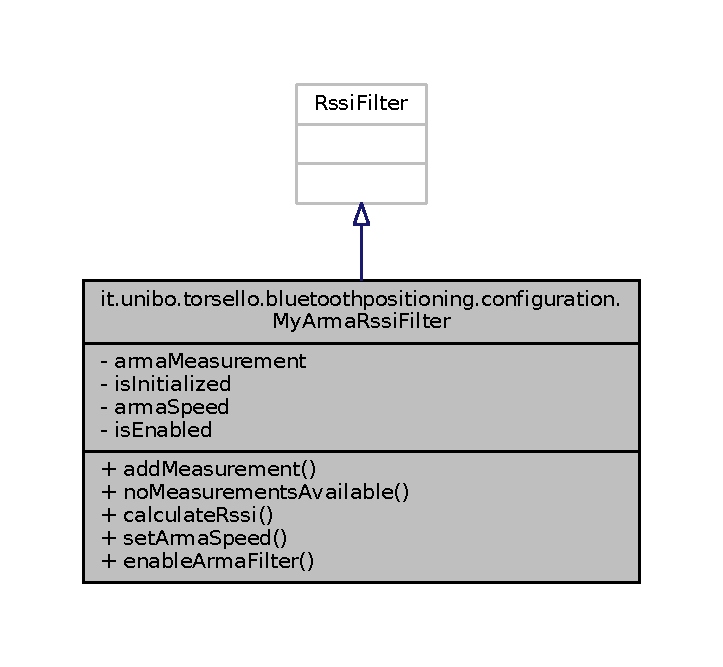
\includegraphics[width=347pt]{classit_1_1unibo_1_1torsello_1_1bluetoothpositioning_1_1configuration_1_1MyArmaRssiFilter__inherit__graph}
\end{center}
\end{figure}


Diagramma di collaborazione per it.\+unibo.\+torsello.\+bluetoothpositioning.\+configuration.\+My\+Arma\+Rssi\+Filter\+:
\nopagebreak
\begin{figure}[H]
\begin{center}
\leavevmode
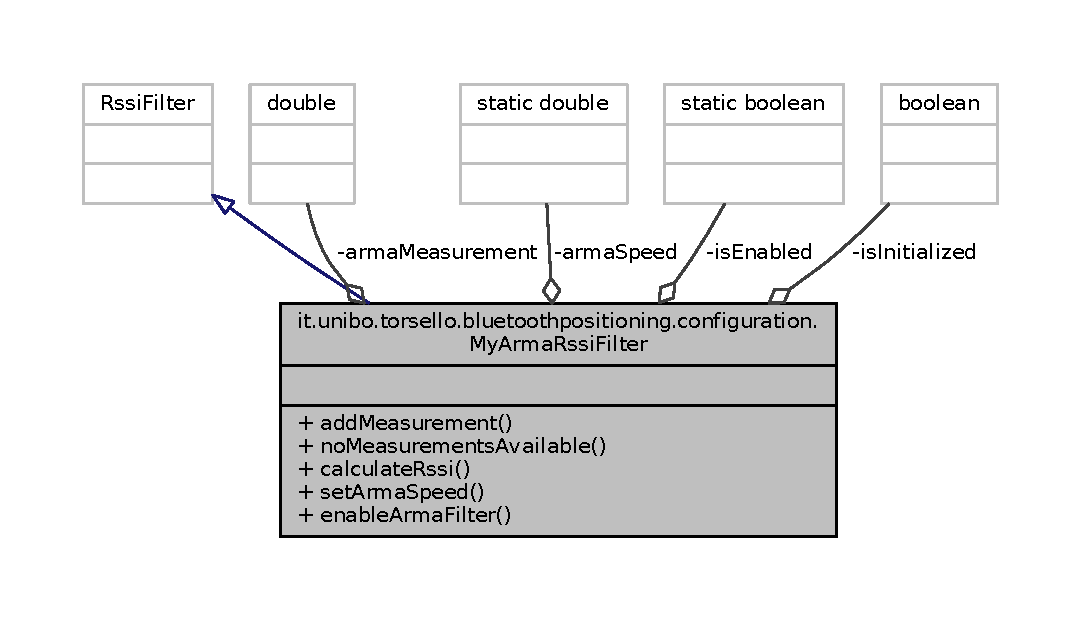
\includegraphics[width=350pt]{classit_1_1unibo_1_1torsello_1_1bluetoothpositioning_1_1configuration_1_1MyArmaRssiFilter__coll__graph}
\end{center}
\end{figure}
\subsubsection*{Membri pubblici}
\begin{DoxyCompactItemize}
\item 
void \hyperlink{classit_1_1unibo_1_1torsello_1_1bluetoothpositioning_1_1configuration_1_1MyArmaRssiFilter_ad35f023bd49df5d11db274ad6a900072_ad35f023bd49df5d11db274ad6a900072}{add\+Measurement} (Integer rssi)
\item 
boolean \hyperlink{classit_1_1unibo_1_1torsello_1_1bluetoothpositioning_1_1configuration_1_1MyArmaRssiFilter_a822204c28f67229cabce721dd39d8cf6_a822204c28f67229cabce721dd39d8cf6}{no\+Measurements\+Available} ()
\item 
double \hyperlink{classit_1_1unibo_1_1torsello_1_1bluetoothpositioning_1_1configuration_1_1MyArmaRssiFilter_afcb40e796f16bc1352d34567e8984a87_afcb40e796f16bc1352d34567e8984a87}{calculate\+Rssi} ()
\end{DoxyCompactItemize}
\subsubsection*{Membri pubblici statici}
\begin{DoxyCompactItemize}
\item 
static void \hyperlink{classit_1_1unibo_1_1torsello_1_1bluetoothpositioning_1_1configuration_1_1MyArmaRssiFilter_a87e5ed9b294bed2cedcbda1ee06bc8ee_a87e5ed9b294bed2cedcbda1ee06bc8ee}{set\+Arma\+Speed} (double arma\+\_\+speed)
\item 
static double \hyperlink{classit_1_1unibo_1_1torsello_1_1bluetoothpositioning_1_1configuration_1_1MyArmaRssiFilter_a91c321ccd7297b3973712cc175f92fa1_a91c321ccd7297b3973712cc175f92fa1}{get\+Arma\+Speed} ()
\item 
static void \hyperlink{classit_1_1unibo_1_1torsello_1_1bluetoothpositioning_1_1configuration_1_1MyArmaRssiFilter_a0ce35b24ad6c6d9abe69e038b3e8da7d_a0ce35b24ad6c6d9abe69e038b3e8da7d}{enable\+Arma\+Filter} (boolean set)
\end{DoxyCompactItemize}
\subsubsection*{Attributi privati}
\begin{DoxyCompactItemize}
\item 
double \hyperlink{classit_1_1unibo_1_1torsello_1_1bluetoothpositioning_1_1configuration_1_1MyArmaRssiFilter_a2be11d7395143321b8f2063afe14a8d0_a2be11d7395143321b8f2063afe14a8d0}{arma\+Measurement}
\item 
boolean \hyperlink{classit_1_1unibo_1_1torsello_1_1bluetoothpositioning_1_1configuration_1_1MyArmaRssiFilter_a01cc7f81fd8e0ca8ed3c197d9fc1fd11_a01cc7f81fd8e0ca8ed3c197d9fc1fd11}{is\+Initialized} = false
\end{DoxyCompactItemize}
\subsubsection*{Attributi privati statici}
\begin{DoxyCompactItemize}
\item 
static double \hyperlink{classit_1_1unibo_1_1torsello_1_1bluetoothpositioning_1_1configuration_1_1MyArmaRssiFilter_a5332b55e26b28536d1f8c7cae5e684b4_a5332b55e26b28536d1f8c7cae5e684b4}{arma\+Speed} = 0.\+1D
\item 
static boolean \hyperlink{classit_1_1unibo_1_1torsello_1_1bluetoothpositioning_1_1configuration_1_1MyArmaRssiFilter_a7a046687ef0d8dd63307cabfbb33fcf8_a7a046687ef0d8dd63307cabfbb33fcf8}{is\+Enabled} = true
\end{DoxyCompactItemize}


\subsubsection{Descrizione dettagliata}
Created by Federico Torsello. \href{mailto:federico.torsello@studio.unibo.it}{\tt federico.\+torsello@studio.\+unibo.\+it} 

\subsubsection{Documentazione delle funzioni membro}
\hypertarget{classit_1_1unibo_1_1torsello_1_1bluetoothpositioning_1_1configuration_1_1MyArmaRssiFilter_ad35f023bd49df5d11db274ad6a900072_ad35f023bd49df5d11db274ad6a900072}{}\label{classit_1_1unibo_1_1torsello_1_1bluetoothpositioning_1_1configuration_1_1MyArmaRssiFilter_ad35f023bd49df5d11db274ad6a900072_ad35f023bd49df5d11db274ad6a900072} 
\index{it\+::unibo\+::torsello\+::bluetoothpositioning\+::configuration\+::\+My\+Arma\+Rssi\+Filter@{it\+::unibo\+::torsello\+::bluetoothpositioning\+::configuration\+::\+My\+Arma\+Rssi\+Filter}!add\+Measurement@{add\+Measurement}}
\index{add\+Measurement@{add\+Measurement}!it\+::unibo\+::torsello\+::bluetoothpositioning\+::configuration\+::\+My\+Arma\+Rssi\+Filter@{it\+::unibo\+::torsello\+::bluetoothpositioning\+::configuration\+::\+My\+Arma\+Rssi\+Filter}}
\paragraph{\texorpdfstring{add\+Measurement()}{addMeasurement()}}
{\footnotesize\ttfamily void it.\+unibo.\+torsello.\+bluetoothpositioning.\+configuration.\+My\+Arma\+Rssi\+Filter.\+add\+Measurement (\begin{DoxyParamCaption}\item[{Integer}]{rssi }\end{DoxyParamCaption})}


\begin{DoxyCode}
30                                              \{
31 
32         \textcolor{keywordflow}{if} (\hyperlink{classit_1_1unibo_1_1torsello_1_1bluetoothpositioning_1_1configuration_1_1MyArmaRssiFilter_a7a046687ef0d8dd63307cabfbb33fcf8_a7a046687ef0d8dd63307cabfbb33fcf8}{isEnabled}) \{
33             \textcolor{keywordflow}{if} (!\hyperlink{classit_1_1unibo_1_1torsello_1_1bluetoothpositioning_1_1configuration_1_1MyArmaRssiFilter_a01cc7f81fd8e0ca8ed3c197d9fc1fd11_a01cc7f81fd8e0ca8ed3c197d9fc1fd11}{isInitialized}) \{
34                 \hyperlink{classit_1_1unibo_1_1torsello_1_1bluetoothpositioning_1_1configuration_1_1MyArmaRssiFilter_a2be11d7395143321b8f2063afe14a8d0_a2be11d7395143321b8f2063afe14a8d0}{armaMeasurement} = rssi;
35                 \hyperlink{classit_1_1unibo_1_1torsello_1_1bluetoothpositioning_1_1configuration_1_1MyArmaRssiFilter_a01cc7f81fd8e0ca8ed3c197d9fc1fd11_a01cc7f81fd8e0ca8ed3c197d9fc1fd11}{isInitialized} = \textcolor{keyword}{true};
36             \}
37 
38             \hyperlink{classit_1_1unibo_1_1torsello_1_1bluetoothpositioning_1_1configuration_1_1MyArmaRssiFilter_a2be11d7395143321b8f2063afe14a8d0_a2be11d7395143321b8f2063afe14a8d0}{armaMeasurement} = (\hyperlink{classit_1_1unibo_1_1torsello_1_1bluetoothpositioning_1_1configuration_1_1MyArmaRssiFilter_a2be11d7395143321b8f2063afe14a8d0_a2be11d7395143321b8f2063afe14a8d0}{armaMeasurement} - 
      \hyperlink{classit_1_1unibo_1_1torsello_1_1bluetoothpositioning_1_1configuration_1_1MyArmaRssiFilter_a5332b55e26b28536d1f8c7cae5e684b4_a5332b55e26b28536d1f8c7cae5e684b4}{armaSpeed} * (\hyperlink{classit_1_1unibo_1_1torsello_1_1bluetoothpositioning_1_1configuration_1_1MyArmaRssiFilter_a2be11d7395143321b8f2063afe14a8d0_a2be11d7395143321b8f2063afe14a8d0}{armaMeasurement} - rssi));
39         \} \textcolor{keywordflow}{else} \{
40             \hyperlink{classit_1_1unibo_1_1torsello_1_1bluetoothpositioning_1_1configuration_1_1MyArmaRssiFilter_a2be11d7395143321b8f2063afe14a8d0_a2be11d7395143321b8f2063afe14a8d0}{armaMeasurement} = rssi;
41         \}
42 
43     \}
\end{DoxyCode}
\hypertarget{classit_1_1unibo_1_1torsello_1_1bluetoothpositioning_1_1configuration_1_1MyArmaRssiFilter_afcb40e796f16bc1352d34567e8984a87_afcb40e796f16bc1352d34567e8984a87}{}\label{classit_1_1unibo_1_1torsello_1_1bluetoothpositioning_1_1configuration_1_1MyArmaRssiFilter_afcb40e796f16bc1352d34567e8984a87_afcb40e796f16bc1352d34567e8984a87} 
\index{it\+::unibo\+::torsello\+::bluetoothpositioning\+::configuration\+::\+My\+Arma\+Rssi\+Filter@{it\+::unibo\+::torsello\+::bluetoothpositioning\+::configuration\+::\+My\+Arma\+Rssi\+Filter}!calculate\+Rssi@{calculate\+Rssi}}
\index{calculate\+Rssi@{calculate\+Rssi}!it\+::unibo\+::torsello\+::bluetoothpositioning\+::configuration\+::\+My\+Arma\+Rssi\+Filter@{it\+::unibo\+::torsello\+::bluetoothpositioning\+::configuration\+::\+My\+Arma\+Rssi\+Filter}}
\paragraph{\texorpdfstring{calculate\+Rssi()}{calculateRssi()}}
{\footnotesize\ttfamily double it.\+unibo.\+torsello.\+bluetoothpositioning.\+configuration.\+My\+Arma\+Rssi\+Filter.\+calculate\+Rssi (\begin{DoxyParamCaption}{ }\end{DoxyParamCaption})}


\begin{DoxyCode}
51                                   \{
52         \textcolor{keywordflow}{return} \hyperlink{classit_1_1unibo_1_1torsello_1_1bluetoothpositioning_1_1configuration_1_1MyArmaRssiFilter_a2be11d7395143321b8f2063afe14a8d0_a2be11d7395143321b8f2063afe14a8d0}{armaMeasurement};
53     \}
\end{DoxyCode}
\hypertarget{classit_1_1unibo_1_1torsello_1_1bluetoothpositioning_1_1configuration_1_1MyArmaRssiFilter_a0ce35b24ad6c6d9abe69e038b3e8da7d_a0ce35b24ad6c6d9abe69e038b3e8da7d}{}\label{classit_1_1unibo_1_1torsello_1_1bluetoothpositioning_1_1configuration_1_1MyArmaRssiFilter_a0ce35b24ad6c6d9abe69e038b3e8da7d_a0ce35b24ad6c6d9abe69e038b3e8da7d} 
\index{it\+::unibo\+::torsello\+::bluetoothpositioning\+::configuration\+::\+My\+Arma\+Rssi\+Filter@{it\+::unibo\+::torsello\+::bluetoothpositioning\+::configuration\+::\+My\+Arma\+Rssi\+Filter}!enable\+Arma\+Filter@{enable\+Arma\+Filter}}
\index{enable\+Arma\+Filter@{enable\+Arma\+Filter}!it\+::unibo\+::torsello\+::bluetoothpositioning\+::configuration\+::\+My\+Arma\+Rssi\+Filter@{it\+::unibo\+::torsello\+::bluetoothpositioning\+::configuration\+::\+My\+Arma\+Rssi\+Filter}}
\paragraph{\texorpdfstring{enable\+Arma\+Filter()}{enableArmaFilter()}}
{\footnotesize\ttfamily static void it.\+unibo.\+torsello.\+bluetoothpositioning.\+configuration.\+My\+Arma\+Rssi\+Filter.\+enable\+Arma\+Filter (\begin{DoxyParamCaption}\item[{boolean}]{set }\end{DoxyParamCaption})\hspace{0.3cm}{\ttfamily [static]}}


\begin{DoxyCode}
25                                                      \{
26         \hyperlink{classit_1_1unibo_1_1torsello_1_1bluetoothpositioning_1_1configuration_1_1MyArmaRssiFilter_a7a046687ef0d8dd63307cabfbb33fcf8_a7a046687ef0d8dd63307cabfbb33fcf8}{isEnabled} = \textcolor{keyword}{set};
27     \}
\end{DoxyCode}
\hypertarget{classit_1_1unibo_1_1torsello_1_1bluetoothpositioning_1_1configuration_1_1MyArmaRssiFilter_a91c321ccd7297b3973712cc175f92fa1_a91c321ccd7297b3973712cc175f92fa1}{}\label{classit_1_1unibo_1_1torsello_1_1bluetoothpositioning_1_1configuration_1_1MyArmaRssiFilter_a91c321ccd7297b3973712cc175f92fa1_a91c321ccd7297b3973712cc175f92fa1} 
\index{it\+::unibo\+::torsello\+::bluetoothpositioning\+::configuration\+::\+My\+Arma\+Rssi\+Filter@{it\+::unibo\+::torsello\+::bluetoothpositioning\+::configuration\+::\+My\+Arma\+Rssi\+Filter}!get\+Arma\+Speed@{get\+Arma\+Speed}}
\index{get\+Arma\+Speed@{get\+Arma\+Speed}!it\+::unibo\+::torsello\+::bluetoothpositioning\+::configuration\+::\+My\+Arma\+Rssi\+Filter@{it\+::unibo\+::torsello\+::bluetoothpositioning\+::configuration\+::\+My\+Arma\+Rssi\+Filter}}
\paragraph{\texorpdfstring{get\+Arma\+Speed()}{getArmaSpeed()}}
{\footnotesize\ttfamily static double it.\+unibo.\+torsello.\+bluetoothpositioning.\+configuration.\+My\+Arma\+Rssi\+Filter.\+get\+Arma\+Speed (\begin{DoxyParamCaption}{ }\end{DoxyParamCaption})\hspace{0.3cm}{\ttfamily [static]}}


\begin{DoxyCode}
21                                         \{
22         \textcolor{keywordflow}{return} \hyperlink{classit_1_1unibo_1_1torsello_1_1bluetoothpositioning_1_1configuration_1_1MyArmaRssiFilter_a5332b55e26b28536d1f8c7cae5e684b4_a5332b55e26b28536d1f8c7cae5e684b4}{armaSpeed};
23     \}
\end{DoxyCode}
\hypertarget{classit_1_1unibo_1_1torsello_1_1bluetoothpositioning_1_1configuration_1_1MyArmaRssiFilter_a822204c28f67229cabce721dd39d8cf6_a822204c28f67229cabce721dd39d8cf6}{}\label{classit_1_1unibo_1_1torsello_1_1bluetoothpositioning_1_1configuration_1_1MyArmaRssiFilter_a822204c28f67229cabce721dd39d8cf6_a822204c28f67229cabce721dd39d8cf6} 
\index{it\+::unibo\+::torsello\+::bluetoothpositioning\+::configuration\+::\+My\+Arma\+Rssi\+Filter@{it\+::unibo\+::torsello\+::bluetoothpositioning\+::configuration\+::\+My\+Arma\+Rssi\+Filter}!no\+Measurements\+Available@{no\+Measurements\+Available}}
\index{no\+Measurements\+Available@{no\+Measurements\+Available}!it\+::unibo\+::torsello\+::bluetoothpositioning\+::configuration\+::\+My\+Arma\+Rssi\+Filter@{it\+::unibo\+::torsello\+::bluetoothpositioning\+::configuration\+::\+My\+Arma\+Rssi\+Filter}}
\paragraph{\texorpdfstring{no\+Measurements\+Available()}{noMeasurementsAvailable()}}
{\footnotesize\ttfamily boolean it.\+unibo.\+torsello.\+bluetoothpositioning.\+configuration.\+My\+Arma\+Rssi\+Filter.\+no\+Measurements\+Available (\begin{DoxyParamCaption}{ }\end{DoxyParamCaption})}


\begin{DoxyCode}
46                                              \{
47         \textcolor{keywordflow}{return} \textcolor{keyword}{false};
48     \}
\end{DoxyCode}
\hypertarget{classit_1_1unibo_1_1torsello_1_1bluetoothpositioning_1_1configuration_1_1MyArmaRssiFilter_a87e5ed9b294bed2cedcbda1ee06bc8ee_a87e5ed9b294bed2cedcbda1ee06bc8ee}{}\label{classit_1_1unibo_1_1torsello_1_1bluetoothpositioning_1_1configuration_1_1MyArmaRssiFilter_a87e5ed9b294bed2cedcbda1ee06bc8ee_a87e5ed9b294bed2cedcbda1ee06bc8ee} 
\index{it\+::unibo\+::torsello\+::bluetoothpositioning\+::configuration\+::\+My\+Arma\+Rssi\+Filter@{it\+::unibo\+::torsello\+::bluetoothpositioning\+::configuration\+::\+My\+Arma\+Rssi\+Filter}!set\+Arma\+Speed@{set\+Arma\+Speed}}
\index{set\+Arma\+Speed@{set\+Arma\+Speed}!it\+::unibo\+::torsello\+::bluetoothpositioning\+::configuration\+::\+My\+Arma\+Rssi\+Filter@{it\+::unibo\+::torsello\+::bluetoothpositioning\+::configuration\+::\+My\+Arma\+Rssi\+Filter}}
\paragraph{\texorpdfstring{set\+Arma\+Speed()}{setArmaSpeed()}}
{\footnotesize\ttfamily static void it.\+unibo.\+torsello.\+bluetoothpositioning.\+configuration.\+My\+Arma\+Rssi\+Filter.\+set\+Arma\+Speed (\begin{DoxyParamCaption}\item[{double}]{arma\+\_\+speed }\end{DoxyParamCaption})\hspace{0.3cm}{\ttfamily [static]}}


\begin{DoxyCode}
17                                                        \{
18         \hyperlink{classit_1_1unibo_1_1torsello_1_1bluetoothpositioning_1_1configuration_1_1MyArmaRssiFilter_a5332b55e26b28536d1f8c7cae5e684b4_a5332b55e26b28536d1f8c7cae5e684b4}{armaSpeed} = arma\_speed;
19     \}
\end{DoxyCode}


\subsubsection{Documentazione dei membri dato}
\hypertarget{classit_1_1unibo_1_1torsello_1_1bluetoothpositioning_1_1configuration_1_1MyArmaRssiFilter_a2be11d7395143321b8f2063afe14a8d0_a2be11d7395143321b8f2063afe14a8d0}{}\label{classit_1_1unibo_1_1torsello_1_1bluetoothpositioning_1_1configuration_1_1MyArmaRssiFilter_a2be11d7395143321b8f2063afe14a8d0_a2be11d7395143321b8f2063afe14a8d0} 
\index{it\+::unibo\+::torsello\+::bluetoothpositioning\+::configuration\+::\+My\+Arma\+Rssi\+Filter@{it\+::unibo\+::torsello\+::bluetoothpositioning\+::configuration\+::\+My\+Arma\+Rssi\+Filter}!arma\+Measurement@{arma\+Measurement}}
\index{arma\+Measurement@{arma\+Measurement}!it\+::unibo\+::torsello\+::bluetoothpositioning\+::configuration\+::\+My\+Arma\+Rssi\+Filter@{it\+::unibo\+::torsello\+::bluetoothpositioning\+::configuration\+::\+My\+Arma\+Rssi\+Filter}}
\paragraph{\texorpdfstring{arma\+Measurement}{armaMeasurement}}
{\footnotesize\ttfamily double it.\+unibo.\+torsello.\+bluetoothpositioning.\+configuration.\+My\+Arma\+Rssi\+Filter.\+arma\+Measurement\hspace{0.3cm}{\ttfamily [private]}}

\hypertarget{classit_1_1unibo_1_1torsello_1_1bluetoothpositioning_1_1configuration_1_1MyArmaRssiFilter_a5332b55e26b28536d1f8c7cae5e684b4_a5332b55e26b28536d1f8c7cae5e684b4}{}\label{classit_1_1unibo_1_1torsello_1_1bluetoothpositioning_1_1configuration_1_1MyArmaRssiFilter_a5332b55e26b28536d1f8c7cae5e684b4_a5332b55e26b28536d1f8c7cae5e684b4} 
\index{it\+::unibo\+::torsello\+::bluetoothpositioning\+::configuration\+::\+My\+Arma\+Rssi\+Filter@{it\+::unibo\+::torsello\+::bluetoothpositioning\+::configuration\+::\+My\+Arma\+Rssi\+Filter}!arma\+Speed@{arma\+Speed}}
\index{arma\+Speed@{arma\+Speed}!it\+::unibo\+::torsello\+::bluetoothpositioning\+::configuration\+::\+My\+Arma\+Rssi\+Filter@{it\+::unibo\+::torsello\+::bluetoothpositioning\+::configuration\+::\+My\+Arma\+Rssi\+Filter}}
\paragraph{\texorpdfstring{arma\+Speed}{armaSpeed}}
{\footnotesize\ttfamily double it.\+unibo.\+torsello.\+bluetoothpositioning.\+configuration.\+My\+Arma\+Rssi\+Filter.\+arma\+Speed = 0.\+1D\hspace{0.3cm}{\ttfamily [static]}, {\ttfamily [private]}}

\hypertarget{classit_1_1unibo_1_1torsello_1_1bluetoothpositioning_1_1configuration_1_1MyArmaRssiFilter_a7a046687ef0d8dd63307cabfbb33fcf8_a7a046687ef0d8dd63307cabfbb33fcf8}{}\label{classit_1_1unibo_1_1torsello_1_1bluetoothpositioning_1_1configuration_1_1MyArmaRssiFilter_a7a046687ef0d8dd63307cabfbb33fcf8_a7a046687ef0d8dd63307cabfbb33fcf8} 
\index{it\+::unibo\+::torsello\+::bluetoothpositioning\+::configuration\+::\+My\+Arma\+Rssi\+Filter@{it\+::unibo\+::torsello\+::bluetoothpositioning\+::configuration\+::\+My\+Arma\+Rssi\+Filter}!is\+Enabled@{is\+Enabled}}
\index{is\+Enabled@{is\+Enabled}!it\+::unibo\+::torsello\+::bluetoothpositioning\+::configuration\+::\+My\+Arma\+Rssi\+Filter@{it\+::unibo\+::torsello\+::bluetoothpositioning\+::configuration\+::\+My\+Arma\+Rssi\+Filter}}
\paragraph{\texorpdfstring{is\+Enabled}{isEnabled}}
{\footnotesize\ttfamily boolean it.\+unibo.\+torsello.\+bluetoothpositioning.\+configuration.\+My\+Arma\+Rssi\+Filter.\+is\+Enabled = true\hspace{0.3cm}{\ttfamily [static]}, {\ttfamily [private]}}

\hypertarget{classit_1_1unibo_1_1torsello_1_1bluetoothpositioning_1_1configuration_1_1MyArmaRssiFilter_a01cc7f81fd8e0ca8ed3c197d9fc1fd11_a01cc7f81fd8e0ca8ed3c197d9fc1fd11}{}\label{classit_1_1unibo_1_1torsello_1_1bluetoothpositioning_1_1configuration_1_1MyArmaRssiFilter_a01cc7f81fd8e0ca8ed3c197d9fc1fd11_a01cc7f81fd8e0ca8ed3c197d9fc1fd11} 
\index{it\+::unibo\+::torsello\+::bluetoothpositioning\+::configuration\+::\+My\+Arma\+Rssi\+Filter@{it\+::unibo\+::torsello\+::bluetoothpositioning\+::configuration\+::\+My\+Arma\+Rssi\+Filter}!is\+Initialized@{is\+Initialized}}
\index{is\+Initialized@{is\+Initialized}!it\+::unibo\+::torsello\+::bluetoothpositioning\+::configuration\+::\+My\+Arma\+Rssi\+Filter@{it\+::unibo\+::torsello\+::bluetoothpositioning\+::configuration\+::\+My\+Arma\+Rssi\+Filter}}
\paragraph{\texorpdfstring{is\+Initialized}{isInitialized}}
{\footnotesize\ttfamily boolean it.\+unibo.\+torsello.\+bluetoothpositioning.\+configuration.\+My\+Arma\+Rssi\+Filter.\+is\+Initialized = false\hspace{0.3cm}{\ttfamily [private]}}



La documentazione per questa classe è stata generata a partire dal seguente file\+:\begin{DoxyCompactItemize}
\item 
\hyperlink{MyArmaRssiFilter_8java}{My\+Arma\+Rssi\+Filter.\+java}\end{DoxyCompactItemize}

\hypertarget{classit_1_1unibo_1_1torsello_1_1bluetoothpositioning_1_1examplesCamera_1_1Preview}{}\subsection{Riferimenti per la classe it.\+unibo.\+torsello.\+bluetoothpositioning.\+examples\+Camera.\+Preview}
\label{classit_1_1unibo_1_1torsello_1_1bluetoothpositioning_1_1examplesCamera_1_1Preview}\index{it.\+unibo.\+torsello.\+bluetoothpositioning.\+examples\+Camera.\+Preview@{it.\+unibo.\+torsello.\+bluetoothpositioning.\+examples\+Camera.\+Preview}}


Diagramma delle classi per it.\+unibo.\+torsello.\+bluetoothpositioning.\+examples\+Camera.\+Preview
\nopagebreak
\begin{figure}[H]
\begin{center}
\leavevmode
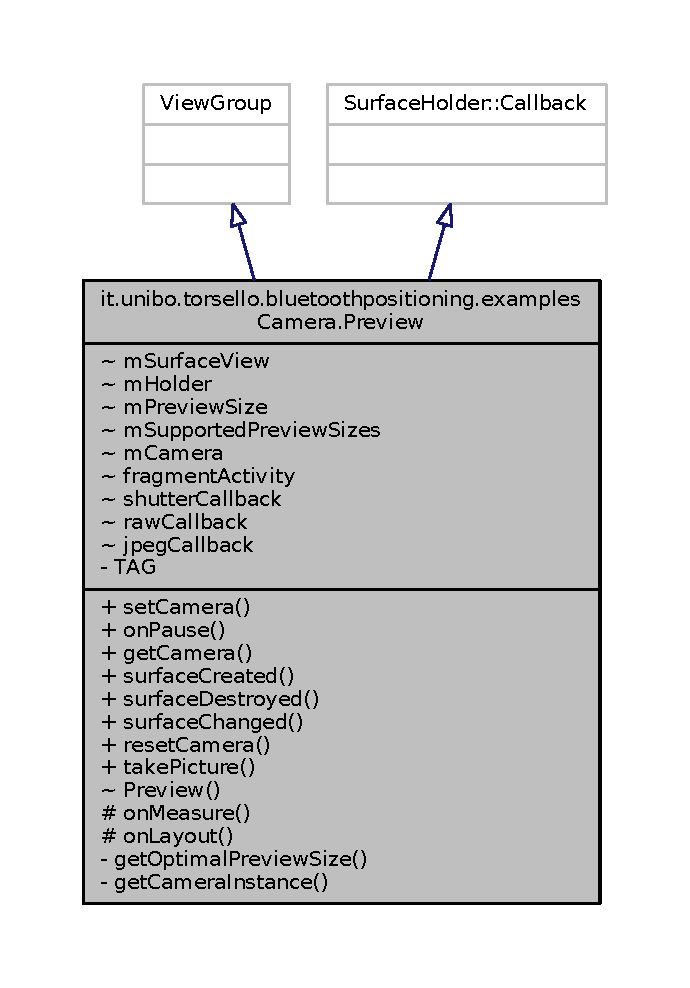
\includegraphics[width=331pt]{classit_1_1unibo_1_1torsello_1_1bluetoothpositioning_1_1examplesCamera_1_1Preview__inherit__graph}
\end{center}
\end{figure}


Diagramma di collaborazione per it.\+unibo.\+torsello.\+bluetoothpositioning.\+examples\+Camera.\+Preview\+:
\nopagebreak
\begin{figure}[H]
\begin{center}
\leavevmode
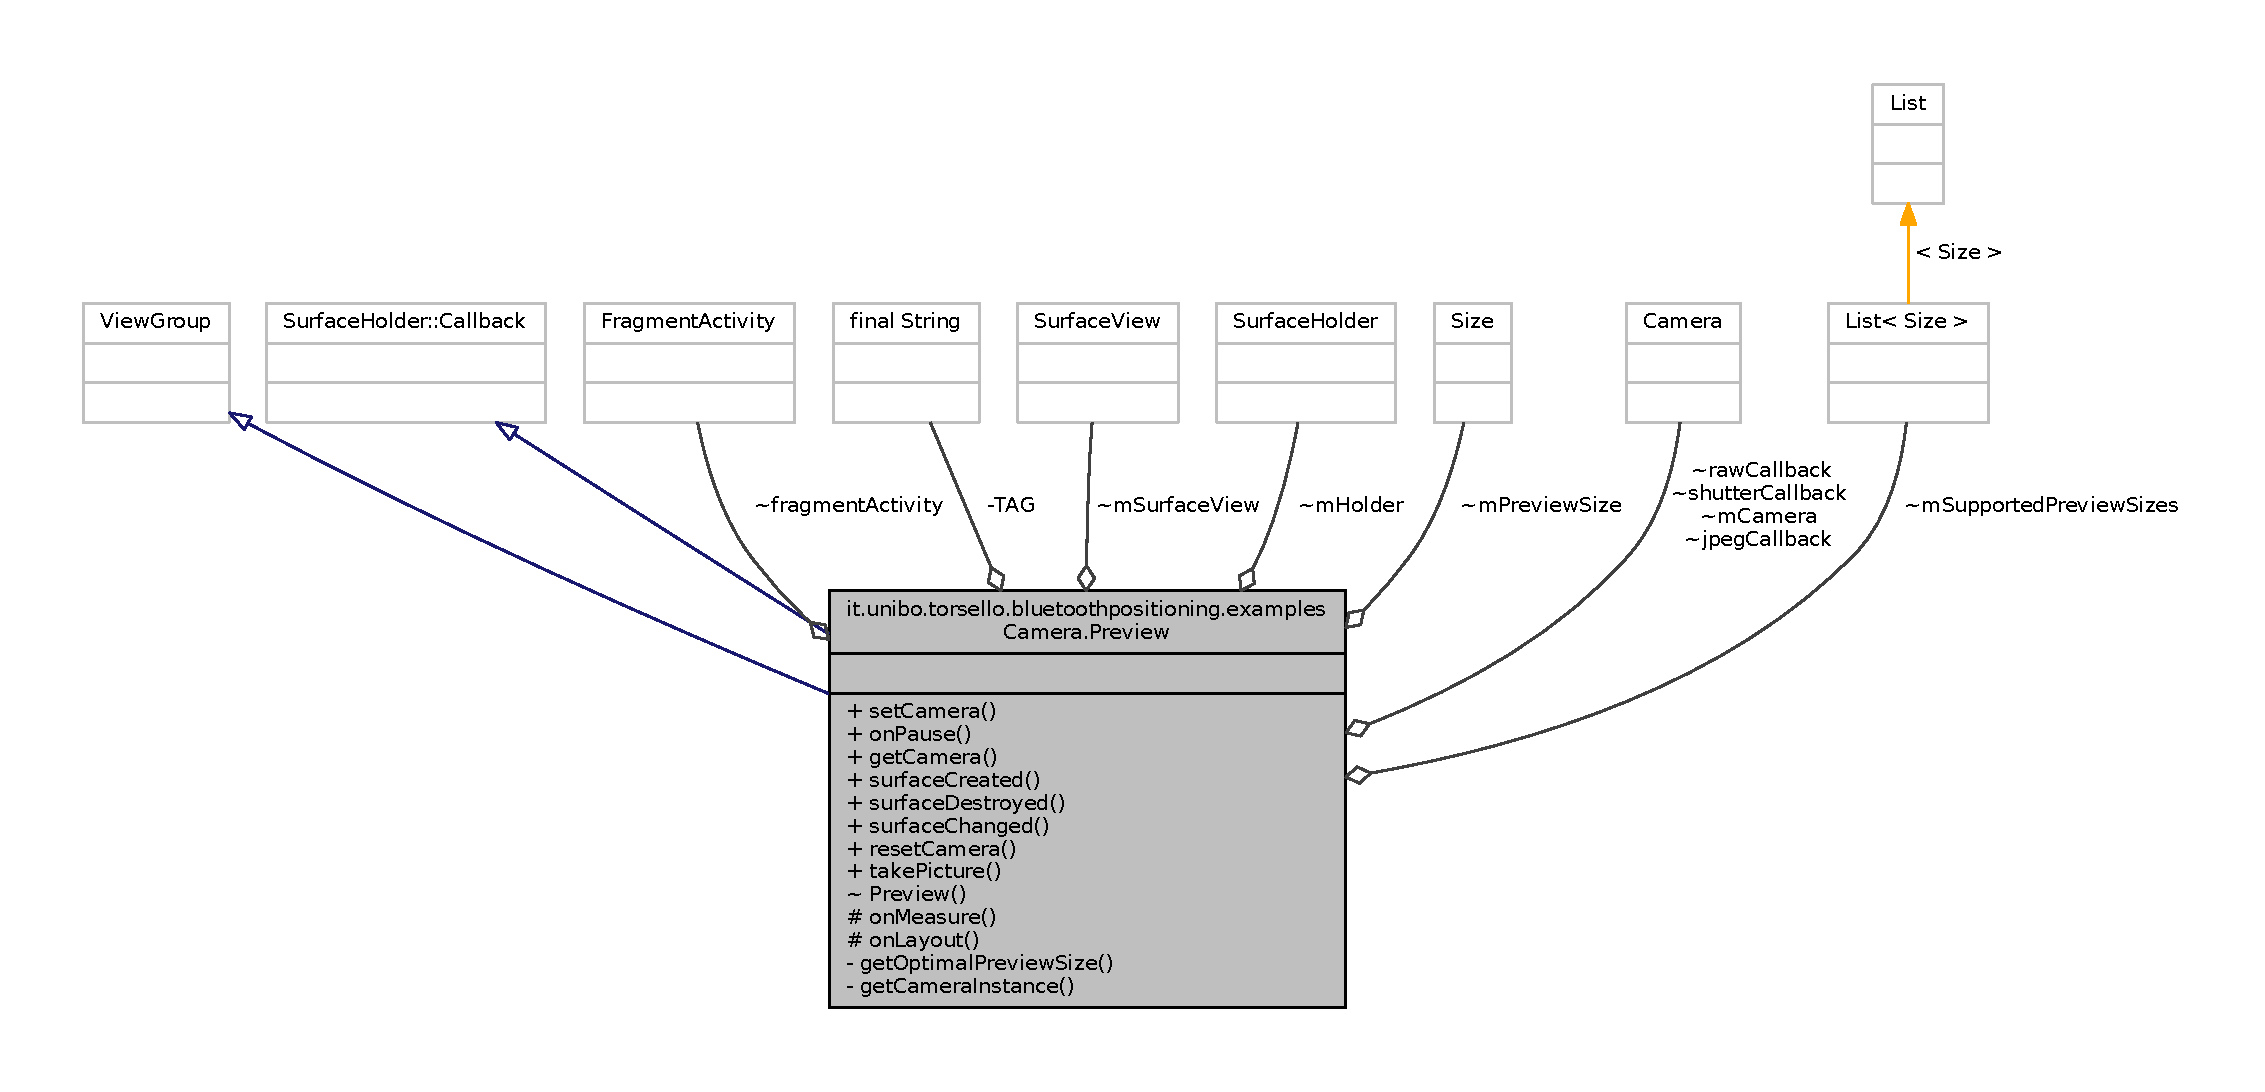
\includegraphics[width=350pt]{classit_1_1unibo_1_1torsello_1_1bluetoothpositioning_1_1examplesCamera_1_1Preview__coll__graph}
\end{center}
\end{figure}
\subsubsection*{Membri pubblici}
\begin{DoxyCompactItemize}
\item 
void \hyperlink{classit_1_1unibo_1_1torsello_1_1bluetoothpositioning_1_1examplesCamera_1_1Preview_a018960081707cd70025fb4b7e0322162_a018960081707cd70025fb4b7e0322162}{set\+Camera} (Fragment\+Activity \hyperlink{classit_1_1unibo_1_1torsello_1_1bluetoothpositioning_1_1examplesCamera_1_1Preview_afb962539b64017465860fcbf9a903370_afb962539b64017465860fcbf9a903370}{fragment\+Activity})
\item 
void \hyperlink{classit_1_1unibo_1_1torsello_1_1bluetoothpositioning_1_1examplesCamera_1_1Preview_af63fabacd267ab2763cc3183464dbf47_af63fabacd267ab2763cc3183464dbf47}{on\+Pause} ()
\item 
Camera \hyperlink{classit_1_1unibo_1_1torsello_1_1bluetoothpositioning_1_1examplesCamera_1_1Preview_a8bc995f4776255800f64dfb94d38e47d_a8bc995f4776255800f64dfb94d38e47d}{get\+Camera} ()
\item 
void \hyperlink{classit_1_1unibo_1_1torsello_1_1bluetoothpositioning_1_1examplesCamera_1_1Preview_afff805882286610f41ac1cb33e19abdc_afff805882286610f41ac1cb33e19abdc}{surface\+Created} (Surface\+Holder holder)
\item 
void \hyperlink{classit_1_1unibo_1_1torsello_1_1bluetoothpositioning_1_1examplesCamera_1_1Preview_abed0494890fb81c8db6d62a28b20434b_abed0494890fb81c8db6d62a28b20434b}{surface\+Destroyed} (Surface\+Holder holder)
\item 
void \hyperlink{classit_1_1unibo_1_1torsello_1_1bluetoothpositioning_1_1examplesCamera_1_1Preview_a05b0be70607a79a5cc710bdb8f9710c8_a05b0be70607a79a5cc710bdb8f9710c8}{surface\+Changed} (Surface\+Holder holder, int format, int w, int h)
\item 
void \hyperlink{classit_1_1unibo_1_1torsello_1_1bluetoothpositioning_1_1examplesCamera_1_1Preview_a26bdf3a50e5e5044510f2ba1583ce8d8_a26bdf3a50e5e5044510f2ba1583ce8d8}{reset\+Camera} ()
\item 
void \hyperlink{classit_1_1unibo_1_1torsello_1_1bluetoothpositioning_1_1examplesCamera_1_1Preview_afa7f533cc47be1bf7be2b1d1bfa43600_afa7f533cc47be1bf7be2b1d1bfa43600}{take\+Picture} ()
\end{DoxyCompactItemize}
\subsubsection*{Membri protetti}
\begin{DoxyCompactItemize}
\item 
void \hyperlink{classit_1_1unibo_1_1torsello_1_1bluetoothpositioning_1_1examplesCamera_1_1Preview_a0006f057eb17dbcbd9555144009c6947_a0006f057eb17dbcbd9555144009c6947}{on\+Measure} (int width\+Measure\+Spec, int height\+Measure\+Spec)
\item 
void \hyperlink{classit_1_1unibo_1_1torsello_1_1bluetoothpositioning_1_1examplesCamera_1_1Preview_a93af42647109198d02609680760ef465_a93af42647109198d02609680760ef465}{on\+Layout} (boolean changed, int l, int t, int r, int b)
\end{DoxyCompactItemize}
\subsubsection*{Funzioni con visibilità di package}
\begin{DoxyCompactItemize}
\item 
\hyperlink{classit_1_1unibo_1_1torsello_1_1bluetoothpositioning_1_1examplesCamera_1_1Preview_ae54d5d8e5125fd0a38b28d9416cc0191_ae54d5d8e5125fd0a38b28d9416cc0191}{Preview} (Context context, Surface\+View sv)
\end{DoxyCompactItemize}
\subsubsection*{Attributi con visibilità di package}
\begin{DoxyCompactItemize}
\item 
Surface\+View \hyperlink{classit_1_1unibo_1_1torsello_1_1bluetoothpositioning_1_1examplesCamera_1_1Preview_ab263548281e75df6638ae313628fa44f_ab263548281e75df6638ae313628fa44f}{m\+Surface\+View}
\item 
Surface\+Holder \hyperlink{classit_1_1unibo_1_1torsello_1_1bluetoothpositioning_1_1examplesCamera_1_1Preview_a2eed693c06e3775f459852371eee7af5_a2eed693c06e3775f459852371eee7af5}{m\+Holder}
\item 
Size \hyperlink{classit_1_1unibo_1_1torsello_1_1bluetoothpositioning_1_1examplesCamera_1_1Preview_a88377f3f6e83780ee72b8cd7af58f139_a88377f3f6e83780ee72b8cd7af58f139}{m\+Preview\+Size}
\item 
List$<$ Size $>$ \hyperlink{classit_1_1unibo_1_1torsello_1_1bluetoothpositioning_1_1examplesCamera_1_1Preview_a791c85132a70dbfdf70587f12753e306_a791c85132a70dbfdf70587f12753e306}{m\+Supported\+Preview\+Sizes}
\item 
Camera \hyperlink{classit_1_1unibo_1_1torsello_1_1bluetoothpositioning_1_1examplesCamera_1_1Preview_a1690c2d132a340b5726ef9712e961dd9_a1690c2d132a340b5726ef9712e961dd9}{m\+Camera}
\item 
Fragment\+Activity \hyperlink{classit_1_1unibo_1_1torsello_1_1bluetoothpositioning_1_1examplesCamera_1_1Preview_afb962539b64017465860fcbf9a903370_afb962539b64017465860fcbf9a903370}{fragment\+Activity}
\item 
Camera.\+Shutter\+Callback \hyperlink{classit_1_1unibo_1_1torsello_1_1bluetoothpositioning_1_1examplesCamera_1_1Preview_a090d01bab1a7e25e77656d17526d6637_a090d01bab1a7e25e77656d17526d6637}{shutter\+Callback}
\item 
Camera.\+Picture\+Callback \hyperlink{classit_1_1unibo_1_1torsello_1_1bluetoothpositioning_1_1examplesCamera_1_1Preview_ab2e159a03a9f9b4fc8733eb645b90617_ab2e159a03a9f9b4fc8733eb645b90617}{raw\+Callback}
\item 
Camera.\+Picture\+Callback \hyperlink{classit_1_1unibo_1_1torsello_1_1bluetoothpositioning_1_1examplesCamera_1_1Preview_a66d23d916709e2283ca48282d29175e4_a66d23d916709e2283ca48282d29175e4}{jpeg\+Callback}
\end{DoxyCompactItemize}
\subsubsection*{Membri privati}
\begin{DoxyCompactItemize}
\item 
Size \hyperlink{classit_1_1unibo_1_1torsello_1_1bluetoothpositioning_1_1examplesCamera_1_1Preview_a46718c866d8f8bc77c5efb98f38e8ad8_a46718c866d8f8bc77c5efb98f38e8ad8}{get\+Optimal\+Preview\+Size} (List$<$ Size $>$ sizes, int w, int h)
\end{DoxyCompactItemize}
\subsubsection*{Membri privati statici}
\begin{DoxyCompactItemize}
\item 
static Camera \hyperlink{classit_1_1unibo_1_1torsello_1_1bluetoothpositioning_1_1examplesCamera_1_1Preview_a89ed563293f04de8313a866702452738_a89ed563293f04de8313a866702452738}{get\+Camera\+Instance} ()
\end{DoxyCompactItemize}
\subsubsection*{Attributi privati}
\begin{DoxyCompactItemize}
\item 
final String \hyperlink{classit_1_1unibo_1_1torsello_1_1bluetoothpositioning_1_1examplesCamera_1_1Preview_a0e05d509a5425eba210e8d1a816c1d42_a0e05d509a5425eba210e8d1a816c1d42}{T\+AG} = \char`\"{}Preview\char`\"{}
\end{DoxyCompactItemize}


\subsubsection{Descrizione dettagliata}
Created by Federico Torsello. \href{mailto:federico.torsello@studio.unibo.it}{\tt federico.\+torsello@studio.\+unibo.\+it} 

\subsubsection{Documentazione dei costruttori e dei distruttori}
\hypertarget{classit_1_1unibo_1_1torsello_1_1bluetoothpositioning_1_1examplesCamera_1_1Preview_ae54d5d8e5125fd0a38b28d9416cc0191_ae54d5d8e5125fd0a38b28d9416cc0191}{}\label{classit_1_1unibo_1_1torsello_1_1bluetoothpositioning_1_1examplesCamera_1_1Preview_ae54d5d8e5125fd0a38b28d9416cc0191_ae54d5d8e5125fd0a38b28d9416cc0191} 
\index{it\+::unibo\+::torsello\+::bluetoothpositioning\+::examples\+Camera\+::\+Preview@{it\+::unibo\+::torsello\+::bluetoothpositioning\+::examples\+Camera\+::\+Preview}!Preview@{Preview}}
\index{Preview@{Preview}!it\+::unibo\+::torsello\+::bluetoothpositioning\+::examples\+Camera\+::\+Preview@{it\+::unibo\+::torsello\+::bluetoothpositioning\+::examples\+Camera\+::\+Preview}}
\paragraph{\texorpdfstring{Preview()}{Preview()}}
{\footnotesize\ttfamily it.\+unibo.\+torsello.\+bluetoothpositioning.\+examples\+Camera.\+Preview.\+Preview (\begin{DoxyParamCaption}\item[{Context}]{context,  }\item[{Surface\+View}]{sv }\end{DoxyParamCaption})\hspace{0.3cm}{\ttfamily [package]}}


\begin{DoxyCode}
32                                              \{
33         super(context);
34 
35 
36         \hyperlink{classit_1_1unibo_1_1torsello_1_1bluetoothpositioning_1_1examplesCamera_1_1Preview_ab263548281e75df6638ae313628fa44f_ab263548281e75df6638ae313628fa44f}{mSurfaceView} = sv;
37 
38         \hyperlink{classit_1_1unibo_1_1torsello_1_1bluetoothpositioning_1_1examplesCamera_1_1Preview_a2eed693c06e3775f459852371eee7af5_a2eed693c06e3775f459852371eee7af5}{mHolder} = \hyperlink{classit_1_1unibo_1_1torsello_1_1bluetoothpositioning_1_1examplesCamera_1_1Preview_ab263548281e75df6638ae313628fa44f_ab263548281e75df6638ae313628fa44f}{mSurfaceView}.getHolder();
39         \hyperlink{classit_1_1unibo_1_1torsello_1_1bluetoothpositioning_1_1examplesCamera_1_1Preview_a2eed693c06e3775f459852371eee7af5_a2eed693c06e3775f459852371eee7af5}{mHolder}.addCallback(\textcolor{keyword}{this});
40         \hyperlink{classit_1_1unibo_1_1torsello_1_1bluetoothpositioning_1_1examplesCamera_1_1Preview_a2eed693c06e3775f459852371eee7af5_a2eed693c06e3775f459852371eee7af5}{mHolder}.setType(SurfaceHolder.SURFACE\_TYPE\_PUSH\_BUFFERS);
41     \}
\end{DoxyCode}


\subsubsection{Documentazione delle funzioni membro}
\hypertarget{classit_1_1unibo_1_1torsello_1_1bluetoothpositioning_1_1examplesCamera_1_1Preview_a8bc995f4776255800f64dfb94d38e47d_a8bc995f4776255800f64dfb94d38e47d}{}\label{classit_1_1unibo_1_1torsello_1_1bluetoothpositioning_1_1examplesCamera_1_1Preview_a8bc995f4776255800f64dfb94d38e47d_a8bc995f4776255800f64dfb94d38e47d} 
\index{it\+::unibo\+::torsello\+::bluetoothpositioning\+::examples\+Camera\+::\+Preview@{it\+::unibo\+::torsello\+::bluetoothpositioning\+::examples\+Camera\+::\+Preview}!get\+Camera@{get\+Camera}}
\index{get\+Camera@{get\+Camera}!it\+::unibo\+::torsello\+::bluetoothpositioning\+::examples\+Camera\+::\+Preview@{it\+::unibo\+::torsello\+::bluetoothpositioning\+::examples\+Camera\+::\+Preview}}
\paragraph{\texorpdfstring{get\+Camera()}{getCamera()}}
{\footnotesize\ttfamily Camera it.\+unibo.\+torsello.\+bluetoothpositioning.\+examples\+Camera.\+Preview.\+get\+Camera (\begin{DoxyParamCaption}{ }\end{DoxyParamCaption})}


\begin{DoxyCode}
79                               \{
80         \textcolor{keywordflow}{return} \hyperlink{classit_1_1unibo_1_1torsello_1_1bluetoothpositioning_1_1examplesCamera_1_1Preview_a1690c2d132a340b5726ef9712e961dd9_a1690c2d132a340b5726ef9712e961dd9}{mCamera};
81     \}
\end{DoxyCode}
\hypertarget{classit_1_1unibo_1_1torsello_1_1bluetoothpositioning_1_1examplesCamera_1_1Preview_a89ed563293f04de8313a866702452738_a89ed563293f04de8313a866702452738}{}\label{classit_1_1unibo_1_1torsello_1_1bluetoothpositioning_1_1examplesCamera_1_1Preview_a89ed563293f04de8313a866702452738_a89ed563293f04de8313a866702452738} 
\index{it\+::unibo\+::torsello\+::bluetoothpositioning\+::examples\+Camera\+::\+Preview@{it\+::unibo\+::torsello\+::bluetoothpositioning\+::examples\+Camera\+::\+Preview}!get\+Camera\+Instance@{get\+Camera\+Instance}}
\index{get\+Camera\+Instance@{get\+Camera\+Instance}!it\+::unibo\+::torsello\+::bluetoothpositioning\+::examples\+Camera\+::\+Preview@{it\+::unibo\+::torsello\+::bluetoothpositioning\+::examples\+Camera\+::\+Preview}}
\paragraph{\texorpdfstring{get\+Camera\+Instance()}{getCameraInstance()}}
{\footnotesize\ttfamily static Camera it.\+unibo.\+torsello.\+bluetoothpositioning.\+examples\+Camera.\+Preview.\+get\+Camera\+Instance (\begin{DoxyParamCaption}{ }\end{DoxyParamCaption})\hspace{0.3cm}{\ttfamily [static]}, {\ttfamily [private]}}

A safe way to get an instance of the Camera\+Util object. 
\begin{DoxyCode}
86                                               \{
87 
88         Camera c = null;
89 
90         \textcolor{keywordflow}{try} \{
91             \textcolor{keywordtype}{int} numCams = Camera.getNumberOfCameras();
92             \textcolor{keywordflow}{if} (numCams > 0) \{
93                 c = Camera.open(0); \textcolor{comment}{// attempt to get a CameraUtil instance}
94             \}
95         \} \textcolor{keywordflow}{catch} (RuntimeException e) \{
96             \textcolor{comment}{// CameraUtil is not available (in use or does not exist)}
97             e.getStackTrace();
98         \}
99 
100         \textcolor{keywordflow}{return} c; \textcolor{comment}{// returns null if camera is unavailable}
101     \}
\end{DoxyCode}
\hypertarget{classit_1_1unibo_1_1torsello_1_1bluetoothpositioning_1_1examplesCamera_1_1Preview_a46718c866d8f8bc77c5efb98f38e8ad8_a46718c866d8f8bc77c5efb98f38e8ad8}{}\label{classit_1_1unibo_1_1torsello_1_1bluetoothpositioning_1_1examplesCamera_1_1Preview_a46718c866d8f8bc77c5efb98f38e8ad8_a46718c866d8f8bc77c5efb98f38e8ad8} 
\index{it\+::unibo\+::torsello\+::bluetoothpositioning\+::examples\+Camera\+::\+Preview@{it\+::unibo\+::torsello\+::bluetoothpositioning\+::examples\+Camera\+::\+Preview}!get\+Optimal\+Preview\+Size@{get\+Optimal\+Preview\+Size}}
\index{get\+Optimal\+Preview\+Size@{get\+Optimal\+Preview\+Size}!it\+::unibo\+::torsello\+::bluetoothpositioning\+::examples\+Camera\+::\+Preview@{it\+::unibo\+::torsello\+::bluetoothpositioning\+::examples\+Camera\+::\+Preview}}
\paragraph{\texorpdfstring{get\+Optimal\+Preview\+Size()}{getOptimalPreviewSize()}}
{\footnotesize\ttfamily Size it.\+unibo.\+torsello.\+bluetoothpositioning.\+examples\+Camera.\+Preview.\+get\+Optimal\+Preview\+Size (\begin{DoxyParamCaption}\item[{List$<$ Size $>$}]{sizes,  }\item[{int}]{w,  }\item[{int}]{h }\end{DoxyParamCaption})\hspace{0.3cm}{\ttfamily [private]}}


\begin{DoxyCode}
167                                                                        \{
168         \textcolor{keyword}{final} \textcolor{keywordtype}{double} ASPECT\_TOLERANCE = 0.1;
169         \textcolor{keywordtype}{double} targetRatio = (double) w / h;
170         \textcolor{keywordflow}{if} (sizes == null) \textcolor{keywordflow}{return} null;
171 
172         Size optimalSize = null;
173         \textcolor{keywordtype}{double} minDiff = Double.MAX\_VALUE;
174 
175 \textcolor{comment}{//        int targetHeight = h;}
176 
177         \textcolor{comment}{// Try to find an size match aspect ratio and size}
178         \textcolor{keywordflow}{for} (Size size : sizes) \{
179             \textcolor{keywordtype}{double} ratio = (double) size.width / size.height;
180             if (Math.abs(ratio - targetRatio) > ASPECT\_TOLERANCE) \textcolor{keywordflow}{continue};
181             \textcolor{keywordflow}{if} (Math.abs(size.height - h) < minDiff) \{
182                 optimalSize = size;
183                 minDiff = Math.abs(size.height - h);
184             \}
185         \}
186 
187         \textcolor{comment}{// Cannot find the one match the aspect ratio, ignore the requirement}
188         \textcolor{keywordflow}{if} (optimalSize == null) \{
189             minDiff = Double.MAX\_VALUE;
190             \textcolor{keywordflow}{for} (Size size : sizes) \{
191                 \textcolor{keywordflow}{if} (Math.abs(size.height - h) < minDiff) \{
192                     optimalSize = size;
193                     minDiff = Math.abs(size.height - h);
194                 \}
195             \}
196         \}
197         \textcolor{keywordflow}{return} optimalSize;
198     \}
\end{DoxyCode}
\hypertarget{classit_1_1unibo_1_1torsello_1_1bluetoothpositioning_1_1examplesCamera_1_1Preview_a93af42647109198d02609680760ef465_a93af42647109198d02609680760ef465}{}\label{classit_1_1unibo_1_1torsello_1_1bluetoothpositioning_1_1examplesCamera_1_1Preview_a93af42647109198d02609680760ef465_a93af42647109198d02609680760ef465} 
\index{it\+::unibo\+::torsello\+::bluetoothpositioning\+::examples\+Camera\+::\+Preview@{it\+::unibo\+::torsello\+::bluetoothpositioning\+::examples\+Camera\+::\+Preview}!on\+Layout@{on\+Layout}}
\index{on\+Layout@{on\+Layout}!it\+::unibo\+::torsello\+::bluetoothpositioning\+::examples\+Camera\+::\+Preview@{it\+::unibo\+::torsello\+::bluetoothpositioning\+::examples\+Camera\+::\+Preview}}
\paragraph{\texorpdfstring{on\+Layout()}{onLayout()}}
{\footnotesize\ttfamily void it.\+unibo.\+torsello.\+bluetoothpositioning.\+examples\+Camera.\+Preview.\+on\+Layout (\begin{DoxyParamCaption}\item[{boolean}]{changed,  }\item[{int}]{l,  }\item[{int}]{t,  }\item[{int}]{r,  }\item[{int}]{b }\end{DoxyParamCaption})\hspace{0.3cm}{\ttfamily [protected]}}


\begin{DoxyCode}
118                                                                          \{
119         \textcolor{keywordflow}{if} (changed && getChildCount() > 0) \{
120             \textcolor{keyword}{final} View child = getChildAt(0);
121 
122             \textcolor{keyword}{final} \textcolor{keywordtype}{int} width = r - l;
123             \textcolor{keyword}{final} \textcolor{keywordtype}{int} height = b - t;
124 
125             \textcolor{keywordtype}{int} previewWidth = width;
126             \textcolor{keywordtype}{int} previewHeight = height;
127             \textcolor{keywordflow}{if} (\hyperlink{classit_1_1unibo_1_1torsello_1_1bluetoothpositioning_1_1examplesCamera_1_1Preview_a88377f3f6e83780ee72b8cd7af58f139_a88377f3f6e83780ee72b8cd7af58f139}{mPreviewSize} != null) \{
128                 previewWidth = \hyperlink{classit_1_1unibo_1_1torsello_1_1bluetoothpositioning_1_1examplesCamera_1_1Preview_a88377f3f6e83780ee72b8cd7af58f139_a88377f3f6e83780ee72b8cd7af58f139}{mPreviewSize}.width;
129                 previewHeight = \hyperlink{classit_1_1unibo_1_1torsello_1_1bluetoothpositioning_1_1examplesCamera_1_1Preview_a88377f3f6e83780ee72b8cd7af58f139_a88377f3f6e83780ee72b8cd7af58f139}{mPreviewSize}.height;
130             \}
131 
132             \textcolor{comment}{// Center the child SurfaceView within the parent.}
133             \textcolor{keywordflow}{if} (width * previewHeight > height * previewWidth) \{
134                 \textcolor{keyword}{final} \textcolor{keywordtype}{int} scaledChildWidth = previewWidth * height / previewHeight;
135                 child.layout((width - scaledChildWidth) / 2, 0,
136                         (width + scaledChildWidth) / 2, height);
137             \} \textcolor{keywordflow}{else} \{
138                 \textcolor{keyword}{final} \textcolor{keywordtype}{int} scaledChildHeight = previewHeight * width / previewWidth;
139                 child.layout(0, (height - scaledChildHeight) / 2,
140                         width, (height + scaledChildHeight) / 2);
141             \}
142         \}
143     \}
\end{DoxyCode}
\hypertarget{classit_1_1unibo_1_1torsello_1_1bluetoothpositioning_1_1examplesCamera_1_1Preview_a0006f057eb17dbcbd9555144009c6947_a0006f057eb17dbcbd9555144009c6947}{}\label{classit_1_1unibo_1_1torsello_1_1bluetoothpositioning_1_1examplesCamera_1_1Preview_a0006f057eb17dbcbd9555144009c6947_a0006f057eb17dbcbd9555144009c6947} 
\index{it\+::unibo\+::torsello\+::bluetoothpositioning\+::examples\+Camera\+::\+Preview@{it\+::unibo\+::torsello\+::bluetoothpositioning\+::examples\+Camera\+::\+Preview}!on\+Measure@{on\+Measure}}
\index{on\+Measure@{on\+Measure}!it\+::unibo\+::torsello\+::bluetoothpositioning\+::examples\+Camera\+::\+Preview@{it\+::unibo\+::torsello\+::bluetoothpositioning\+::examples\+Camera\+::\+Preview}}
\paragraph{\texorpdfstring{on\+Measure()}{onMeasure()}}
{\footnotesize\ttfamily void it.\+unibo.\+torsello.\+bluetoothpositioning.\+examples\+Camera.\+Preview.\+on\+Measure (\begin{DoxyParamCaption}\item[{int}]{width\+Measure\+Spec,  }\item[{int}]{height\+Measure\+Spec }\end{DoxyParamCaption})\hspace{0.3cm}{\ttfamily [protected]}}


\begin{DoxyCode}
104                                                                           \{
105         \textcolor{comment}{// We purposely disregard child measurements because act as a}
106         \textcolor{comment}{// wrapper to a SurfaceView that centers the camera preview instead}
107         \textcolor{comment}{// of stretching it.}
108         \textcolor{keyword}{final} \textcolor{keywordtype}{int} width = resolveSize(getSuggestedMinimumWidth(), widthMeasureSpec);
109         \textcolor{keyword}{final} \textcolor{keywordtype}{int} height = resolveSize(getSuggestedMinimumHeight(), heightMeasureSpec);
110         setMeasuredDimension(width, height);
111 
112         \textcolor{keywordflow}{if} (\hyperlink{classit_1_1unibo_1_1torsello_1_1bluetoothpositioning_1_1examplesCamera_1_1Preview_a791c85132a70dbfdf70587f12753e306_a791c85132a70dbfdf70587f12753e306}{mSupportedPreviewSizes} != null) \{
113             \hyperlink{classit_1_1unibo_1_1torsello_1_1bluetoothpositioning_1_1examplesCamera_1_1Preview_a88377f3f6e83780ee72b8cd7af58f139_a88377f3f6e83780ee72b8cd7af58f139}{mPreviewSize} = \hyperlink{classit_1_1unibo_1_1torsello_1_1bluetoothpositioning_1_1examplesCamera_1_1Preview_a46718c866d8f8bc77c5efb98f38e8ad8_a46718c866d8f8bc77c5efb98f38e8ad8}{getOptimalPreviewSize}(
      \hyperlink{classit_1_1unibo_1_1torsello_1_1bluetoothpositioning_1_1examplesCamera_1_1Preview_a791c85132a70dbfdf70587f12753e306_a791c85132a70dbfdf70587f12753e306}{mSupportedPreviewSizes}, width, height);
114         \}
115     \}
\end{DoxyCode}
\hypertarget{classit_1_1unibo_1_1torsello_1_1bluetoothpositioning_1_1examplesCamera_1_1Preview_af63fabacd267ab2763cc3183464dbf47_af63fabacd267ab2763cc3183464dbf47}{}\label{classit_1_1unibo_1_1torsello_1_1bluetoothpositioning_1_1examplesCamera_1_1Preview_af63fabacd267ab2763cc3183464dbf47_af63fabacd267ab2763cc3183464dbf47} 
\index{it\+::unibo\+::torsello\+::bluetoothpositioning\+::examples\+Camera\+::\+Preview@{it\+::unibo\+::torsello\+::bluetoothpositioning\+::examples\+Camera\+::\+Preview}!on\+Pause@{on\+Pause}}
\index{on\+Pause@{on\+Pause}!it\+::unibo\+::torsello\+::bluetoothpositioning\+::examples\+Camera\+::\+Preview@{it\+::unibo\+::torsello\+::bluetoothpositioning\+::examples\+Camera\+::\+Preview}}
\paragraph{\texorpdfstring{on\+Pause()}{onPause()}}
{\footnotesize\ttfamily void it.\+unibo.\+torsello.\+bluetoothpositioning.\+examples\+Camera.\+Preview.\+on\+Pause (\begin{DoxyParamCaption}{ }\end{DoxyParamCaption})}


\begin{DoxyCode}
71                           \{
72         \textcolor{keywordflow}{if} (\hyperlink{classit_1_1unibo_1_1torsello_1_1bluetoothpositioning_1_1examplesCamera_1_1Preview_a1690c2d132a340b5726ef9712e961dd9_a1690c2d132a340b5726ef9712e961dd9}{mCamera} != null) \{
73             \hyperlink{classit_1_1unibo_1_1torsello_1_1bluetoothpositioning_1_1examplesCamera_1_1Preview_a1690c2d132a340b5726ef9712e961dd9_a1690c2d132a340b5726ef9712e961dd9}{mCamera}.stopPreview();
74             \hyperlink{classit_1_1unibo_1_1torsello_1_1bluetoothpositioning_1_1examplesCamera_1_1Preview_a1690c2d132a340b5726ef9712e961dd9_a1690c2d132a340b5726ef9712e961dd9}{mCamera}.release();
75             \hyperlink{classit_1_1unibo_1_1torsello_1_1bluetoothpositioning_1_1examplesCamera_1_1Preview_a1690c2d132a340b5726ef9712e961dd9_a1690c2d132a340b5726ef9712e961dd9}{mCamera} = null;
76         \}
77     \}
\end{DoxyCode}
\hypertarget{classit_1_1unibo_1_1torsello_1_1bluetoothpositioning_1_1examplesCamera_1_1Preview_a26bdf3a50e5e5044510f2ba1583ce8d8_a26bdf3a50e5e5044510f2ba1583ce8d8}{}\label{classit_1_1unibo_1_1torsello_1_1bluetoothpositioning_1_1examplesCamera_1_1Preview_a26bdf3a50e5e5044510f2ba1583ce8d8_a26bdf3a50e5e5044510f2ba1583ce8d8} 
\index{it\+::unibo\+::torsello\+::bluetoothpositioning\+::examples\+Camera\+::\+Preview@{it\+::unibo\+::torsello\+::bluetoothpositioning\+::examples\+Camera\+::\+Preview}!reset\+Camera@{reset\+Camera}}
\index{reset\+Camera@{reset\+Camera}!it\+::unibo\+::torsello\+::bluetoothpositioning\+::examples\+Camera\+::\+Preview@{it\+::unibo\+::torsello\+::bluetoothpositioning\+::examples\+Camera\+::\+Preview}}
\paragraph{\texorpdfstring{reset\+Camera()}{resetCamera()}}
{\footnotesize\ttfamily void it.\+unibo.\+torsello.\+bluetoothpositioning.\+examples\+Camera.\+Preview.\+reset\+Camera (\begin{DoxyParamCaption}{ }\end{DoxyParamCaption})}


\begin{DoxyCode}
213                               \{
214         \textcolor{keyword}{new} Thread(\textcolor{keyword}{new} Runnable() \{
215             @Override
216             \textcolor{keyword}{public} \textcolor{keywordtype}{void} run() \{
217                 \hyperlink{classit_1_1unibo_1_1torsello_1_1bluetoothpositioning_1_1examplesCamera_1_1Preview_a1690c2d132a340b5726ef9712e961dd9_a1690c2d132a340b5726ef9712e961dd9}{mCamera}.startPreview();
218             \}
219         \}).start();
220 
221 
222     \}
\end{DoxyCode}
\hypertarget{classit_1_1unibo_1_1torsello_1_1bluetoothpositioning_1_1examplesCamera_1_1Preview_a018960081707cd70025fb4b7e0322162_a018960081707cd70025fb4b7e0322162}{}\label{classit_1_1unibo_1_1torsello_1_1bluetoothpositioning_1_1examplesCamera_1_1Preview_a018960081707cd70025fb4b7e0322162_a018960081707cd70025fb4b7e0322162} 
\index{it\+::unibo\+::torsello\+::bluetoothpositioning\+::examples\+Camera\+::\+Preview@{it\+::unibo\+::torsello\+::bluetoothpositioning\+::examples\+Camera\+::\+Preview}!set\+Camera@{set\+Camera}}
\index{set\+Camera@{set\+Camera}!it\+::unibo\+::torsello\+::bluetoothpositioning\+::examples\+Camera\+::\+Preview@{it\+::unibo\+::torsello\+::bluetoothpositioning\+::examples\+Camera\+::\+Preview}}
\paragraph{\texorpdfstring{set\+Camera()}{setCamera()}}
{\footnotesize\ttfamily void it.\+unibo.\+torsello.\+bluetoothpositioning.\+examples\+Camera.\+Preview.\+set\+Camera (\begin{DoxyParamCaption}\item[{Fragment\+Activity}]{fragment\+Activity }\end{DoxyParamCaption})}


\begin{DoxyCode}
43                                                              \{
44 
45         this.\hyperlink{classit_1_1unibo_1_1torsello_1_1bluetoothpositioning_1_1examplesCamera_1_1Preview_afb962539b64017465860fcbf9a903370_afb962539b64017465860fcbf9a903370}{fragmentActivity} = \hyperlink{classit_1_1unibo_1_1torsello_1_1bluetoothpositioning_1_1examplesCamera_1_1Preview_afb962539b64017465860fcbf9a903370_afb962539b64017465860fcbf9a903370}{fragmentActivity};
46         \textcolor{keywordflow}{try} \{
47             \hyperlink{classit_1_1unibo_1_1torsello_1_1bluetoothpositioning_1_1examplesCamera_1_1Preview_a1690c2d132a340b5726ef9712e961dd9_a1690c2d132a340b5726ef9712e961dd9}{mCamera} = \hyperlink{classit_1_1unibo_1_1torsello_1_1bluetoothpositioning_1_1examplesCamera_1_1Preview_a89ed563293f04de8313a866702452738_a89ed563293f04de8313a866702452738}{getCameraInstance}();
48         \} \textcolor{keywordflow}{catch} (RuntimeException ex) \{
49             Toast.makeText(\hyperlink{classit_1_1unibo_1_1torsello_1_1bluetoothpositioning_1_1examplesCamera_1_1Preview_afb962539b64017465860fcbf9a903370_afb962539b64017465860fcbf9a903370}{fragmentActivity}, \textcolor{stringliteral}{"camera\_not\_found"}, Toast.LENGTH\_LONG).show();
50         \}
51 
52         \textcolor{keywordflow}{if} (\hyperlink{classit_1_1unibo_1_1torsello_1_1bluetoothpositioning_1_1examplesCamera_1_1Preview_a1690c2d132a340b5726ef9712e961dd9_a1690c2d132a340b5726ef9712e961dd9}{mCamera} != null) \{
53 
54             \hyperlink{classit_1_1unibo_1_1torsello_1_1bluetoothpositioning_1_1examplesCamera_1_1Preview_a791c85132a70dbfdf70587f12753e306_a791c85132a70dbfdf70587f12753e306}{mSupportedPreviewSizes} = \hyperlink{classit_1_1unibo_1_1torsello_1_1bluetoothpositioning_1_1examplesCamera_1_1Preview_a1690c2d132a340b5726ef9712e961dd9_a1690c2d132a340b5726ef9712e961dd9}{mCamera}.getParameters().
      getSupportedPreviewSizes();
55             requestLayout();
56 
57             \textcolor{comment}{// get Camera parameters}
58             Camera.Parameters params = \hyperlink{classit_1_1unibo_1_1torsello_1_1bluetoothpositioning_1_1examplesCamera_1_1Preview_a1690c2d132a340b5726ef9712e961dd9_a1690c2d132a340b5726ef9712e961dd9}{mCamera}.getParameters();
59 
60             List<String> focusModes = params.getSupportedFocusModes();
61             \textcolor{keywordflow}{if} (focusModes.contains(Camera.Parameters.FOCUS\_MODE\_AUTO)) \{
62                 \textcolor{comment}{// set the focus mode}
63                 params.setFocusMode(Camera.Parameters.FOCUS\_MODE\_AUTO);
64                 \textcolor{comment}{// set Camera parameters}
65                 \hyperlink{classit_1_1unibo_1_1torsello_1_1bluetoothpositioning_1_1examplesCamera_1_1Preview_a1690c2d132a340b5726ef9712e961dd9_a1690c2d132a340b5726ef9712e961dd9}{mCamera}.setParameters(params);
66             \}
67         \}
68 
69     \}
\end{DoxyCode}
\hypertarget{classit_1_1unibo_1_1torsello_1_1bluetoothpositioning_1_1examplesCamera_1_1Preview_a05b0be70607a79a5cc710bdb8f9710c8_a05b0be70607a79a5cc710bdb8f9710c8}{}\label{classit_1_1unibo_1_1torsello_1_1bluetoothpositioning_1_1examplesCamera_1_1Preview_a05b0be70607a79a5cc710bdb8f9710c8_a05b0be70607a79a5cc710bdb8f9710c8} 
\index{it\+::unibo\+::torsello\+::bluetoothpositioning\+::examples\+Camera\+::\+Preview@{it\+::unibo\+::torsello\+::bluetoothpositioning\+::examples\+Camera\+::\+Preview}!surface\+Changed@{surface\+Changed}}
\index{surface\+Changed@{surface\+Changed}!it\+::unibo\+::torsello\+::bluetoothpositioning\+::examples\+Camera\+::\+Preview@{it\+::unibo\+::torsello\+::bluetoothpositioning\+::examples\+Camera\+::\+Preview}}
\paragraph{\texorpdfstring{surface\+Changed()}{surfaceChanged()}}
{\footnotesize\ttfamily void it.\+unibo.\+torsello.\+bluetoothpositioning.\+examples\+Camera.\+Preview.\+surface\+Changed (\begin{DoxyParamCaption}\item[{Surface\+Holder}]{holder,  }\item[{int}]{format,  }\item[{int}]{w,  }\item[{int}]{h }\end{DoxyParamCaption})}


\begin{DoxyCode}
201                                                                                \{
202         \textcolor{keywordflow}{if} (\hyperlink{classit_1_1unibo_1_1torsello_1_1bluetoothpositioning_1_1examplesCamera_1_1Preview_a1690c2d132a340b5726ef9712e961dd9_a1690c2d132a340b5726ef9712e961dd9}{mCamera} != null) \{
203             Camera.Parameters parameters = \hyperlink{classit_1_1unibo_1_1torsello_1_1bluetoothpositioning_1_1examplesCamera_1_1Preview_a1690c2d132a340b5726ef9712e961dd9_a1690c2d132a340b5726ef9712e961dd9}{mCamera}.getParameters();
204             parameters.setPreviewSize(\hyperlink{classit_1_1unibo_1_1torsello_1_1bluetoothpositioning_1_1examplesCamera_1_1Preview_a88377f3f6e83780ee72b8cd7af58f139_a88377f3f6e83780ee72b8cd7af58f139}{mPreviewSize}.width, 
      \hyperlink{classit_1_1unibo_1_1torsello_1_1bluetoothpositioning_1_1examplesCamera_1_1Preview_a88377f3f6e83780ee72b8cd7af58f139_a88377f3f6e83780ee72b8cd7af58f139}{mPreviewSize}.height);
205             requestLayout();
206 
207             \hyperlink{classit_1_1unibo_1_1torsello_1_1bluetoothpositioning_1_1examplesCamera_1_1Preview_a1690c2d132a340b5726ef9712e961dd9_a1690c2d132a340b5726ef9712e961dd9}{mCamera}.setParameters(parameters);
208 
209             \hyperlink{classit_1_1unibo_1_1torsello_1_1bluetoothpositioning_1_1examplesCamera_1_1Preview_a26bdf3a50e5e5044510f2ba1583ce8d8_a26bdf3a50e5e5044510f2ba1583ce8d8}{resetCamera}();
210         \}
211     \}
\end{DoxyCode}
\hypertarget{classit_1_1unibo_1_1torsello_1_1bluetoothpositioning_1_1examplesCamera_1_1Preview_afff805882286610f41ac1cb33e19abdc_afff805882286610f41ac1cb33e19abdc}{}\label{classit_1_1unibo_1_1torsello_1_1bluetoothpositioning_1_1examplesCamera_1_1Preview_afff805882286610f41ac1cb33e19abdc_afff805882286610f41ac1cb33e19abdc} 
\index{it\+::unibo\+::torsello\+::bluetoothpositioning\+::examples\+Camera\+::\+Preview@{it\+::unibo\+::torsello\+::bluetoothpositioning\+::examples\+Camera\+::\+Preview}!surface\+Created@{surface\+Created}}
\index{surface\+Created@{surface\+Created}!it\+::unibo\+::torsello\+::bluetoothpositioning\+::examples\+Camera\+::\+Preview@{it\+::unibo\+::torsello\+::bluetoothpositioning\+::examples\+Camera\+::\+Preview}}
\paragraph{\texorpdfstring{surface\+Created()}{surfaceCreated()}}
{\footnotesize\ttfamily void it.\+unibo.\+torsello.\+bluetoothpositioning.\+examples\+Camera.\+Preview.\+surface\+Created (\begin{DoxyParamCaption}\item[{Surface\+Holder}]{holder }\end{DoxyParamCaption})}


\begin{DoxyCode}
146                                                      \{
147         \textcolor{comment}{// The Surface has been created, acquire the camera and tell it where}
148         \textcolor{comment}{// to draw.}
149         \textcolor{keywordflow}{try} \{
150             \textcolor{keywordflow}{if} (\hyperlink{classit_1_1unibo_1_1torsello_1_1bluetoothpositioning_1_1examplesCamera_1_1Preview_a1690c2d132a340b5726ef9712e961dd9_a1690c2d132a340b5726ef9712e961dd9}{mCamera} != null) \{
151                 \hyperlink{classit_1_1unibo_1_1torsello_1_1bluetoothpositioning_1_1examplesCamera_1_1Preview_a1690c2d132a340b5726ef9712e961dd9_a1690c2d132a340b5726ef9712e961dd9}{mCamera}.setPreviewDisplay(holder);
152             \}
153         \} \textcolor{keywordflow}{catch} (IOException exception) \{
154             Log.e(\hyperlink{classit_1_1unibo_1_1torsello_1_1bluetoothpositioning_1_1examplesCamera_1_1Preview_a0e05d509a5425eba210e8d1a816c1d42_a0e05d509a5425eba210e8d1a816c1d42}{TAG}, \textcolor{stringliteral}{"IOException caused by setPreviewDisplay()"}, exception);
155         \}
156     \}
\end{DoxyCode}
\hypertarget{classit_1_1unibo_1_1torsello_1_1bluetoothpositioning_1_1examplesCamera_1_1Preview_abed0494890fb81c8db6d62a28b20434b_abed0494890fb81c8db6d62a28b20434b}{}\label{classit_1_1unibo_1_1torsello_1_1bluetoothpositioning_1_1examplesCamera_1_1Preview_abed0494890fb81c8db6d62a28b20434b_abed0494890fb81c8db6d62a28b20434b} 
\index{it\+::unibo\+::torsello\+::bluetoothpositioning\+::examples\+Camera\+::\+Preview@{it\+::unibo\+::torsello\+::bluetoothpositioning\+::examples\+Camera\+::\+Preview}!surface\+Destroyed@{surface\+Destroyed}}
\index{surface\+Destroyed@{surface\+Destroyed}!it\+::unibo\+::torsello\+::bluetoothpositioning\+::examples\+Camera\+::\+Preview@{it\+::unibo\+::torsello\+::bluetoothpositioning\+::examples\+Camera\+::\+Preview}}
\paragraph{\texorpdfstring{surface\+Destroyed()}{surfaceDestroyed()}}
{\footnotesize\ttfamily void it.\+unibo.\+torsello.\+bluetoothpositioning.\+examples\+Camera.\+Preview.\+surface\+Destroyed (\begin{DoxyParamCaption}\item[{Surface\+Holder}]{holder }\end{DoxyParamCaption})}


\begin{DoxyCode}
159                                                        \{
160         \textcolor{comment}{// Surface will be destroyed when we return, so stop the preview.}
161         \textcolor{keywordflow}{if} (\hyperlink{classit_1_1unibo_1_1torsello_1_1bluetoothpositioning_1_1examplesCamera_1_1Preview_a1690c2d132a340b5726ef9712e961dd9_a1690c2d132a340b5726ef9712e961dd9}{mCamera} != null) \{
162             \hyperlink{classit_1_1unibo_1_1torsello_1_1bluetoothpositioning_1_1examplesCamera_1_1Preview_a1690c2d132a340b5726ef9712e961dd9_a1690c2d132a340b5726ef9712e961dd9}{mCamera}.stopPreview();
163         \}
164     \}
\end{DoxyCode}
\hypertarget{classit_1_1unibo_1_1torsello_1_1bluetoothpositioning_1_1examplesCamera_1_1Preview_afa7f533cc47be1bf7be2b1d1bfa43600_afa7f533cc47be1bf7be2b1d1bfa43600}{}\label{classit_1_1unibo_1_1torsello_1_1bluetoothpositioning_1_1examplesCamera_1_1Preview_afa7f533cc47be1bf7be2b1d1bfa43600_afa7f533cc47be1bf7be2b1d1bfa43600} 
\index{it\+::unibo\+::torsello\+::bluetoothpositioning\+::examples\+Camera\+::\+Preview@{it\+::unibo\+::torsello\+::bluetoothpositioning\+::examples\+Camera\+::\+Preview}!take\+Picture@{take\+Picture}}
\index{take\+Picture@{take\+Picture}!it\+::unibo\+::torsello\+::bluetoothpositioning\+::examples\+Camera\+::\+Preview@{it\+::unibo\+::torsello\+::bluetoothpositioning\+::examples\+Camera\+::\+Preview}}
\paragraph{\texorpdfstring{take\+Picture()}{takePicture()}}
{\footnotesize\ttfamily void it.\+unibo.\+torsello.\+bluetoothpositioning.\+examples\+Camera.\+Preview.\+take\+Picture (\begin{DoxyParamCaption}{ }\end{DoxyParamCaption})}


\begin{DoxyCode}
246                               \{
247 
248         \hyperlink{classit_1_1unibo_1_1torsello_1_1bluetoothpositioning_1_1examplesCamera_1_1Preview_a1690c2d132a340b5726ef9712e961dd9_a1690c2d132a340b5726ef9712e961dd9}{mCamera}.takePicture(\hyperlink{classit_1_1unibo_1_1torsello_1_1bluetoothpositioning_1_1examplesCamera_1_1Preview_a090d01bab1a7e25e77656d17526d6637_a090d01bab1a7e25e77656d17526d6637}{shutterCallback}, \hyperlink{classit_1_1unibo_1_1torsello_1_1bluetoothpositioning_1_1examplesCamera_1_1Preview_ab2e159a03a9f9b4fc8733eb645b90617_ab2e159a03a9f9b4fc8733eb645b90617}{rawCallback}, 
      \hyperlink{classit_1_1unibo_1_1torsello_1_1bluetoothpositioning_1_1examplesCamera_1_1Preview_a66d23d916709e2283ca48282d29175e4_a66d23d916709e2283ca48282d29175e4}{jpegCallback});
249     \}
\end{DoxyCode}


\subsubsection{Documentazione dei membri dato}
\hypertarget{classit_1_1unibo_1_1torsello_1_1bluetoothpositioning_1_1examplesCamera_1_1Preview_afb962539b64017465860fcbf9a903370_afb962539b64017465860fcbf9a903370}{}\label{classit_1_1unibo_1_1torsello_1_1bluetoothpositioning_1_1examplesCamera_1_1Preview_afb962539b64017465860fcbf9a903370_afb962539b64017465860fcbf9a903370} 
\index{it\+::unibo\+::torsello\+::bluetoothpositioning\+::examples\+Camera\+::\+Preview@{it\+::unibo\+::torsello\+::bluetoothpositioning\+::examples\+Camera\+::\+Preview}!fragment\+Activity@{fragment\+Activity}}
\index{fragment\+Activity@{fragment\+Activity}!it\+::unibo\+::torsello\+::bluetoothpositioning\+::examples\+Camera\+::\+Preview@{it\+::unibo\+::torsello\+::bluetoothpositioning\+::examples\+Camera\+::\+Preview}}
\paragraph{\texorpdfstring{fragment\+Activity}{fragmentActivity}}
{\footnotesize\ttfamily Fragment\+Activity it.\+unibo.\+torsello.\+bluetoothpositioning.\+examples\+Camera.\+Preview.\+fragment\+Activity\hspace{0.3cm}{\ttfamily [package]}}

\hypertarget{classit_1_1unibo_1_1torsello_1_1bluetoothpositioning_1_1examplesCamera_1_1Preview_a66d23d916709e2283ca48282d29175e4_a66d23d916709e2283ca48282d29175e4}{}\label{classit_1_1unibo_1_1torsello_1_1bluetoothpositioning_1_1examplesCamera_1_1Preview_a66d23d916709e2283ca48282d29175e4_a66d23d916709e2283ca48282d29175e4} 
\index{it\+::unibo\+::torsello\+::bluetoothpositioning\+::examples\+Camera\+::\+Preview@{it\+::unibo\+::torsello\+::bluetoothpositioning\+::examples\+Camera\+::\+Preview}!jpeg\+Callback@{jpeg\+Callback}}
\index{jpeg\+Callback@{jpeg\+Callback}!it\+::unibo\+::torsello\+::bluetoothpositioning\+::examples\+Camera\+::\+Preview@{it\+::unibo\+::torsello\+::bluetoothpositioning\+::examples\+Camera\+::\+Preview}}
\paragraph{\texorpdfstring{jpeg\+Callback}{jpegCallback}}
{\footnotesize\ttfamily Camera.\+Picture\+Callback it.\+unibo.\+torsello.\+bluetoothpositioning.\+examples\+Camera.\+Preview.\+jpeg\+Callback\hspace{0.3cm}{\ttfamily [package]}}

{\bfseries Valore iniziale\+:}
\begin{DoxyCode}
= \textcolor{keyword}{new} Camera.PictureCallback() \{
        \textcolor{keyword}{public} \textcolor{keywordtype}{void} onPictureTaken(byte[] data, \textcolor{keyword}{final} Camera camera) \{
            \textcolor{keyword}{new} SaveImageTask(\hyperlink{classit_1_1unibo_1_1torsello_1_1bluetoothpositioning_1_1examplesCamera_1_1Preview_afb962539b64017465860fcbf9a903370_afb962539b64017465860fcbf9a903370}{fragmentActivity}).execute(data);

            \hyperlink{classit_1_1unibo_1_1torsello_1_1bluetoothpositioning_1_1examplesCamera_1_1Preview_a26bdf3a50e5e5044510f2ba1583ce8d8_a26bdf3a50e5e5044510f2ba1583ce8d8}{resetCamera}();

            Log.d(\hyperlink{classit_1_1unibo_1_1torsello_1_1bluetoothpositioning_1_1examplesCamera_1_1Preview_a0e05d509a5425eba210e8d1a816c1d42_a0e05d509a5425eba210e8d1a816c1d42}{TAG}, \textcolor{stringliteral}{"onPictureTaken - jpeg"});
        \}
    \}
\end{DoxyCode}
\hypertarget{classit_1_1unibo_1_1torsello_1_1bluetoothpositioning_1_1examplesCamera_1_1Preview_a1690c2d132a340b5726ef9712e961dd9_a1690c2d132a340b5726ef9712e961dd9}{}\label{classit_1_1unibo_1_1torsello_1_1bluetoothpositioning_1_1examplesCamera_1_1Preview_a1690c2d132a340b5726ef9712e961dd9_a1690c2d132a340b5726ef9712e961dd9} 
\index{it\+::unibo\+::torsello\+::bluetoothpositioning\+::examples\+Camera\+::\+Preview@{it\+::unibo\+::torsello\+::bluetoothpositioning\+::examples\+Camera\+::\+Preview}!m\+Camera@{m\+Camera}}
\index{m\+Camera@{m\+Camera}!it\+::unibo\+::torsello\+::bluetoothpositioning\+::examples\+Camera\+::\+Preview@{it\+::unibo\+::torsello\+::bluetoothpositioning\+::examples\+Camera\+::\+Preview}}
\paragraph{\texorpdfstring{m\+Camera}{mCamera}}
{\footnotesize\ttfamily Camera it.\+unibo.\+torsello.\+bluetoothpositioning.\+examples\+Camera.\+Preview.\+m\+Camera\hspace{0.3cm}{\ttfamily [package]}}

\hypertarget{classit_1_1unibo_1_1torsello_1_1bluetoothpositioning_1_1examplesCamera_1_1Preview_a2eed693c06e3775f459852371eee7af5_a2eed693c06e3775f459852371eee7af5}{}\label{classit_1_1unibo_1_1torsello_1_1bluetoothpositioning_1_1examplesCamera_1_1Preview_a2eed693c06e3775f459852371eee7af5_a2eed693c06e3775f459852371eee7af5} 
\index{it\+::unibo\+::torsello\+::bluetoothpositioning\+::examples\+Camera\+::\+Preview@{it\+::unibo\+::torsello\+::bluetoothpositioning\+::examples\+Camera\+::\+Preview}!m\+Holder@{m\+Holder}}
\index{m\+Holder@{m\+Holder}!it\+::unibo\+::torsello\+::bluetoothpositioning\+::examples\+Camera\+::\+Preview@{it\+::unibo\+::torsello\+::bluetoothpositioning\+::examples\+Camera\+::\+Preview}}
\paragraph{\texorpdfstring{m\+Holder}{mHolder}}
{\footnotesize\ttfamily Surface\+Holder it.\+unibo.\+torsello.\+bluetoothpositioning.\+examples\+Camera.\+Preview.\+m\+Holder\hspace{0.3cm}{\ttfamily [package]}}

\hypertarget{classit_1_1unibo_1_1torsello_1_1bluetoothpositioning_1_1examplesCamera_1_1Preview_a88377f3f6e83780ee72b8cd7af58f139_a88377f3f6e83780ee72b8cd7af58f139}{}\label{classit_1_1unibo_1_1torsello_1_1bluetoothpositioning_1_1examplesCamera_1_1Preview_a88377f3f6e83780ee72b8cd7af58f139_a88377f3f6e83780ee72b8cd7af58f139} 
\index{it\+::unibo\+::torsello\+::bluetoothpositioning\+::examples\+Camera\+::\+Preview@{it\+::unibo\+::torsello\+::bluetoothpositioning\+::examples\+Camera\+::\+Preview}!m\+Preview\+Size@{m\+Preview\+Size}}
\index{m\+Preview\+Size@{m\+Preview\+Size}!it\+::unibo\+::torsello\+::bluetoothpositioning\+::examples\+Camera\+::\+Preview@{it\+::unibo\+::torsello\+::bluetoothpositioning\+::examples\+Camera\+::\+Preview}}
\paragraph{\texorpdfstring{m\+Preview\+Size}{mPreviewSize}}
{\footnotesize\ttfamily Size it.\+unibo.\+torsello.\+bluetoothpositioning.\+examples\+Camera.\+Preview.\+m\+Preview\+Size\hspace{0.3cm}{\ttfamily [package]}}

\hypertarget{classit_1_1unibo_1_1torsello_1_1bluetoothpositioning_1_1examplesCamera_1_1Preview_a791c85132a70dbfdf70587f12753e306_a791c85132a70dbfdf70587f12753e306}{}\label{classit_1_1unibo_1_1torsello_1_1bluetoothpositioning_1_1examplesCamera_1_1Preview_a791c85132a70dbfdf70587f12753e306_a791c85132a70dbfdf70587f12753e306} 
\index{it\+::unibo\+::torsello\+::bluetoothpositioning\+::examples\+Camera\+::\+Preview@{it\+::unibo\+::torsello\+::bluetoothpositioning\+::examples\+Camera\+::\+Preview}!m\+Supported\+Preview\+Sizes@{m\+Supported\+Preview\+Sizes}}
\index{m\+Supported\+Preview\+Sizes@{m\+Supported\+Preview\+Sizes}!it\+::unibo\+::torsello\+::bluetoothpositioning\+::examples\+Camera\+::\+Preview@{it\+::unibo\+::torsello\+::bluetoothpositioning\+::examples\+Camera\+::\+Preview}}
\paragraph{\texorpdfstring{m\+Supported\+Preview\+Sizes}{mSupportedPreviewSizes}}
{\footnotesize\ttfamily List$<$Size$>$ it.\+unibo.\+torsello.\+bluetoothpositioning.\+examples\+Camera.\+Preview.\+m\+Supported\+Preview\+Sizes\hspace{0.3cm}{\ttfamily [package]}}

\hypertarget{classit_1_1unibo_1_1torsello_1_1bluetoothpositioning_1_1examplesCamera_1_1Preview_ab263548281e75df6638ae313628fa44f_ab263548281e75df6638ae313628fa44f}{}\label{classit_1_1unibo_1_1torsello_1_1bluetoothpositioning_1_1examplesCamera_1_1Preview_ab263548281e75df6638ae313628fa44f_ab263548281e75df6638ae313628fa44f} 
\index{it\+::unibo\+::torsello\+::bluetoothpositioning\+::examples\+Camera\+::\+Preview@{it\+::unibo\+::torsello\+::bluetoothpositioning\+::examples\+Camera\+::\+Preview}!m\+Surface\+View@{m\+Surface\+View}}
\index{m\+Surface\+View@{m\+Surface\+View}!it\+::unibo\+::torsello\+::bluetoothpositioning\+::examples\+Camera\+::\+Preview@{it\+::unibo\+::torsello\+::bluetoothpositioning\+::examples\+Camera\+::\+Preview}}
\paragraph{\texorpdfstring{m\+Surface\+View}{mSurfaceView}}
{\footnotesize\ttfamily Surface\+View it.\+unibo.\+torsello.\+bluetoothpositioning.\+examples\+Camera.\+Preview.\+m\+Surface\+View\hspace{0.3cm}{\ttfamily [package]}}

\hypertarget{classit_1_1unibo_1_1torsello_1_1bluetoothpositioning_1_1examplesCamera_1_1Preview_ab2e159a03a9f9b4fc8733eb645b90617_ab2e159a03a9f9b4fc8733eb645b90617}{}\label{classit_1_1unibo_1_1torsello_1_1bluetoothpositioning_1_1examplesCamera_1_1Preview_ab2e159a03a9f9b4fc8733eb645b90617_ab2e159a03a9f9b4fc8733eb645b90617} 
\index{it\+::unibo\+::torsello\+::bluetoothpositioning\+::examples\+Camera\+::\+Preview@{it\+::unibo\+::torsello\+::bluetoothpositioning\+::examples\+Camera\+::\+Preview}!raw\+Callback@{raw\+Callback}}
\index{raw\+Callback@{raw\+Callback}!it\+::unibo\+::torsello\+::bluetoothpositioning\+::examples\+Camera\+::\+Preview@{it\+::unibo\+::torsello\+::bluetoothpositioning\+::examples\+Camera\+::\+Preview}}
\paragraph{\texorpdfstring{raw\+Callback}{rawCallback}}
{\footnotesize\ttfamily Camera.\+Picture\+Callback it.\+unibo.\+torsello.\+bluetoothpositioning.\+examples\+Camera.\+Preview.\+raw\+Callback\hspace{0.3cm}{\ttfamily [package]}}

{\bfseries Valore iniziale\+:}
\begin{DoxyCode}
= \textcolor{keyword}{new} Camera.PictureCallback() \{
        \textcolor{keyword}{public} \textcolor{keywordtype}{void} onPictureTaken(byte[] data, Camera camera) \{
            
        \}
    \}
\end{DoxyCode}
\hypertarget{classit_1_1unibo_1_1torsello_1_1bluetoothpositioning_1_1examplesCamera_1_1Preview_a090d01bab1a7e25e77656d17526d6637_a090d01bab1a7e25e77656d17526d6637}{}\label{classit_1_1unibo_1_1torsello_1_1bluetoothpositioning_1_1examplesCamera_1_1Preview_a090d01bab1a7e25e77656d17526d6637_a090d01bab1a7e25e77656d17526d6637} 
\index{it\+::unibo\+::torsello\+::bluetoothpositioning\+::examples\+Camera\+::\+Preview@{it\+::unibo\+::torsello\+::bluetoothpositioning\+::examples\+Camera\+::\+Preview}!shutter\+Callback@{shutter\+Callback}}
\index{shutter\+Callback@{shutter\+Callback}!it\+::unibo\+::torsello\+::bluetoothpositioning\+::examples\+Camera\+::\+Preview@{it\+::unibo\+::torsello\+::bluetoothpositioning\+::examples\+Camera\+::\+Preview}}
\paragraph{\texorpdfstring{shutter\+Callback}{shutterCallback}}
{\footnotesize\ttfamily Camera.\+Shutter\+Callback it.\+unibo.\+torsello.\+bluetoothpositioning.\+examples\+Camera.\+Preview.\+shutter\+Callback\hspace{0.3cm}{\ttfamily [package]}}

{\bfseries Valore iniziale\+:}
\begin{DoxyCode}
= \textcolor{keyword}{new} Camera.ShutterCallback() \{
        \textcolor{keyword}{public} \textcolor{keywordtype}{void} onShutter() \{
            
        \}
    \}
\end{DoxyCode}
\hypertarget{classit_1_1unibo_1_1torsello_1_1bluetoothpositioning_1_1examplesCamera_1_1Preview_a0e05d509a5425eba210e8d1a816c1d42_a0e05d509a5425eba210e8d1a816c1d42}{}\label{classit_1_1unibo_1_1torsello_1_1bluetoothpositioning_1_1examplesCamera_1_1Preview_a0e05d509a5425eba210e8d1a816c1d42_a0e05d509a5425eba210e8d1a816c1d42} 
\index{it\+::unibo\+::torsello\+::bluetoothpositioning\+::examples\+Camera\+::\+Preview@{it\+::unibo\+::torsello\+::bluetoothpositioning\+::examples\+Camera\+::\+Preview}!T\+AG@{T\+AG}}
\index{T\+AG@{T\+AG}!it\+::unibo\+::torsello\+::bluetoothpositioning\+::examples\+Camera\+::\+Preview@{it\+::unibo\+::torsello\+::bluetoothpositioning\+::examples\+Camera\+::\+Preview}}
\paragraph{\texorpdfstring{T\+AG}{TAG}}
{\footnotesize\ttfamily final String it.\+unibo.\+torsello.\+bluetoothpositioning.\+examples\+Camera.\+Preview.\+T\+AG = \char`\"{}Preview\char`\"{}\hspace{0.3cm}{\ttfamily [private]}}



La documentazione per questa classe è stata generata a partire dal seguente file\+:\begin{DoxyCompactItemize}
\item 
\hyperlink{Preview_8java}{Preview.\+java}\end{DoxyCompactItemize}

\hypertarget{classit_1_1unibo_1_1torsello_1_1bluetoothpositioning_1_1examplesCamera_1_1SaveImageTask}{}\subsection{Riferimenti per la classe it.\+unibo.\+torsello.\+bluetoothpositioning.\+examples\+Camera.\+Save\+Image\+Task}
\label{classit_1_1unibo_1_1torsello_1_1bluetoothpositioning_1_1examplesCamera_1_1SaveImageTask}\index{it.\+unibo.\+torsello.\+bluetoothpositioning.\+examples\+Camera.\+Save\+Image\+Task@{it.\+unibo.\+torsello.\+bluetoothpositioning.\+examples\+Camera.\+Save\+Image\+Task}}


Diagramma delle classi per it.\+unibo.\+torsello.\+bluetoothpositioning.\+examples\+Camera.\+Save\+Image\+Task
\nopagebreak
\begin{figure}[H]
\begin{center}
\leavevmode
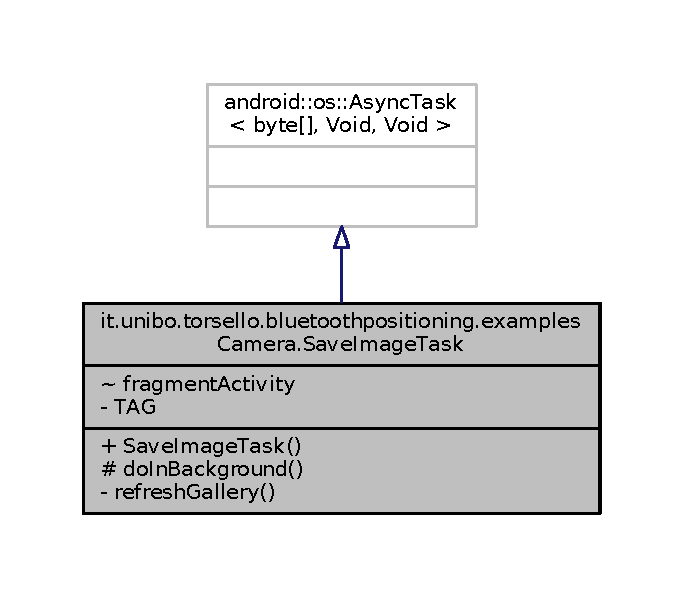
\includegraphics[width=328pt]{classit_1_1unibo_1_1torsello_1_1bluetoothpositioning_1_1examplesCamera_1_1SaveImageTask__inherit__graph}
\end{center}
\end{figure}


Diagramma di collaborazione per it.\+unibo.\+torsello.\+bluetoothpositioning.\+examples\+Camera.\+Save\+Image\+Task\+:
\nopagebreak
\begin{figure}[H]
\begin{center}
\leavevmode
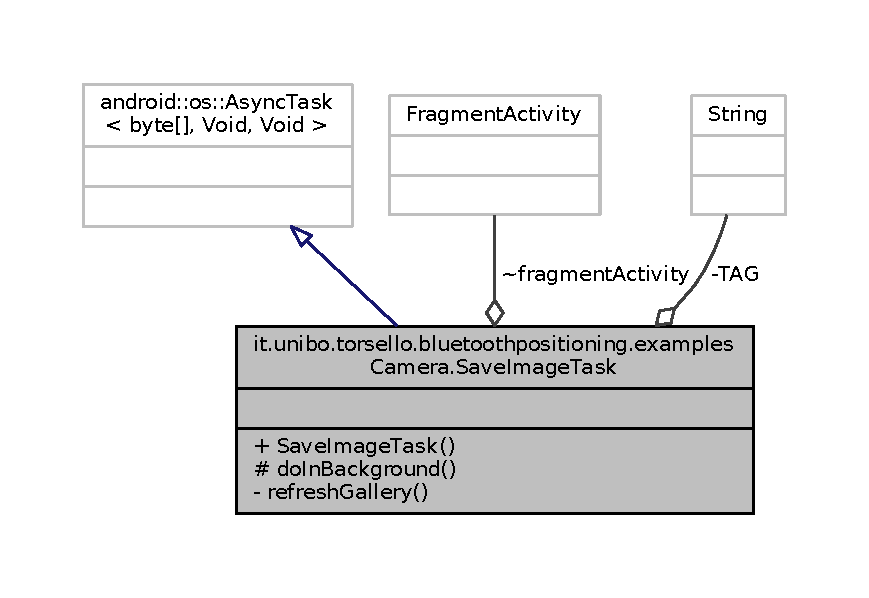
\includegraphics[width=350pt]{classit_1_1unibo_1_1torsello_1_1bluetoothpositioning_1_1examplesCamera_1_1SaveImageTask__coll__graph}
\end{center}
\end{figure}
\subsubsection*{Membri pubblici}
\begin{DoxyCompactItemize}
\item 
\hyperlink{classit_1_1unibo_1_1torsello_1_1bluetoothpositioning_1_1examplesCamera_1_1SaveImageTask_a8d08d12c0e15cc34f4dbfcefc0931629_a8d08d12c0e15cc34f4dbfcefc0931629}{Save\+Image\+Task} (Fragment\+Activity \hyperlink{classit_1_1unibo_1_1torsello_1_1bluetoothpositioning_1_1examplesCamera_1_1SaveImageTask_a020c67ae36b7f908c900da193d9cd110_a020c67ae36b7f908c900da193d9cd110}{fragment\+Activity})
\end{DoxyCompactItemize}
\subsubsection*{Membri protetti}
\begin{DoxyCompactItemize}
\item 
Void \hyperlink{classit_1_1unibo_1_1torsello_1_1bluetoothpositioning_1_1examplesCamera_1_1SaveImageTask_ae71e769fead7e2ec11d99922e03a14d9_ae71e769fead7e2ec11d99922e03a14d9}{do\+In\+Background} (byte\mbox{[}$\,$\mbox{]}... data)
\end{DoxyCompactItemize}
\subsubsection*{Attributi con visibilità di package}
\begin{DoxyCompactItemize}
\item 
Fragment\+Activity \hyperlink{classit_1_1unibo_1_1torsello_1_1bluetoothpositioning_1_1examplesCamera_1_1SaveImageTask_a020c67ae36b7f908c900da193d9cd110_a020c67ae36b7f908c900da193d9cd110}{fragment\+Activity}
\end{DoxyCompactItemize}
\subsubsection*{Membri privati}
\begin{DoxyCompactItemize}
\item 
void \hyperlink{classit_1_1unibo_1_1torsello_1_1bluetoothpositioning_1_1examplesCamera_1_1SaveImageTask_a8bcd9bba7269b952dd0a06bdc3381c25_a8bcd9bba7269b952dd0a06bdc3381c25}{refresh\+Gallery} (File file)
\end{DoxyCompactItemize}
\subsubsection*{Attributi privati statici}
\begin{DoxyCompactItemize}
\item 
static final String \hyperlink{classit_1_1unibo_1_1torsello_1_1bluetoothpositioning_1_1examplesCamera_1_1SaveImageTask_a908ad84901185def0257ea5288f64c3c_a908ad84901185def0257ea5288f64c3c}{T\+AG} = \char`\"{}Save\+Image\+Task\char`\"{}
\end{DoxyCompactItemize}


\subsubsection{Descrizione dettagliata}
Created by Federico Torsello. \href{mailto:federico.torsello@studio.unibo.it}{\tt federico.\+torsello@studio.\+unibo.\+it} 

\subsubsection{Documentazione dei costruttori e dei distruttori}
\hypertarget{classit_1_1unibo_1_1torsello_1_1bluetoothpositioning_1_1examplesCamera_1_1SaveImageTask_a8d08d12c0e15cc34f4dbfcefc0931629_a8d08d12c0e15cc34f4dbfcefc0931629}{}\label{classit_1_1unibo_1_1torsello_1_1bluetoothpositioning_1_1examplesCamera_1_1SaveImageTask_a8d08d12c0e15cc34f4dbfcefc0931629_a8d08d12c0e15cc34f4dbfcefc0931629} 
\index{it\+::unibo\+::torsello\+::bluetoothpositioning\+::examples\+Camera\+::\+Save\+Image\+Task@{it\+::unibo\+::torsello\+::bluetoothpositioning\+::examples\+Camera\+::\+Save\+Image\+Task}!Save\+Image\+Task@{Save\+Image\+Task}}
\index{Save\+Image\+Task@{Save\+Image\+Task}!it\+::unibo\+::torsello\+::bluetoothpositioning\+::examples\+Camera\+::\+Save\+Image\+Task@{it\+::unibo\+::torsello\+::bluetoothpositioning\+::examples\+Camera\+::\+Save\+Image\+Task}}
\paragraph{\texorpdfstring{Save\+Image\+Task()}{SaveImageTask()}}
{\footnotesize\ttfamily it.\+unibo.\+torsello.\+bluetoothpositioning.\+examples\+Camera.\+Save\+Image\+Task.\+Save\+Image\+Task (\begin{DoxyParamCaption}\item[{Fragment\+Activity}]{fragment\+Activity }\end{DoxyParamCaption})}


\begin{DoxyCode}
24                                                             \{
25         this.\hyperlink{classit_1_1unibo_1_1torsello_1_1bluetoothpositioning_1_1examplesCamera_1_1SaveImageTask_a020c67ae36b7f908c900da193d9cd110_a020c67ae36b7f908c900da193d9cd110}{fragmentActivity} = \hyperlink{classit_1_1unibo_1_1torsello_1_1bluetoothpositioning_1_1examplesCamera_1_1SaveImageTask_a020c67ae36b7f908c900da193d9cd110_a020c67ae36b7f908c900da193d9cd110}{fragmentActivity};
26     \}
\end{DoxyCode}


\subsubsection{Documentazione delle funzioni membro}
\hypertarget{classit_1_1unibo_1_1torsello_1_1bluetoothpositioning_1_1examplesCamera_1_1SaveImageTask_ae71e769fead7e2ec11d99922e03a14d9_ae71e769fead7e2ec11d99922e03a14d9}{}\label{classit_1_1unibo_1_1torsello_1_1bluetoothpositioning_1_1examplesCamera_1_1SaveImageTask_ae71e769fead7e2ec11d99922e03a14d9_ae71e769fead7e2ec11d99922e03a14d9} 
\index{it\+::unibo\+::torsello\+::bluetoothpositioning\+::examples\+Camera\+::\+Save\+Image\+Task@{it\+::unibo\+::torsello\+::bluetoothpositioning\+::examples\+Camera\+::\+Save\+Image\+Task}!do\+In\+Background@{do\+In\+Background}}
\index{do\+In\+Background@{do\+In\+Background}!it\+::unibo\+::torsello\+::bluetoothpositioning\+::examples\+Camera\+::\+Save\+Image\+Task@{it\+::unibo\+::torsello\+::bluetoothpositioning\+::examples\+Camera\+::\+Save\+Image\+Task}}
\paragraph{\texorpdfstring{do\+In\+Background()}{doInBackground()}}
{\footnotesize\ttfamily Void it.\+unibo.\+torsello.\+bluetoothpositioning.\+examples\+Camera.\+Save\+Image\+Task.\+do\+In\+Background (\begin{DoxyParamCaption}\item[{byte... \mbox{[}$\,$\mbox{]}}]{data }\end{DoxyParamCaption})\hspace{0.3cm}{\ttfamily [protected]}}


\begin{DoxyCode}
29                                                   \{
30 
31         \textcolor{comment}{// Write to SD Card}
32         \textcolor{keywordflow}{try} \{
33             File sdCard = Environment.getExternalStorageDirectory();
34             File dir = \textcolor{keyword}{new} File(sdCard.getAbsolutePath() + \textcolor{stringliteral}{"/camtest"});
35 \textcolor{comment}{//                    dir.mkdirs();}
36 
37             String fileName = String.format(Locale.getDefault(), \textcolor{stringliteral}{"%d.jpg"}, System.currentTimeMillis());
38             File outFile = \textcolor{keyword}{new} File(dir, fileName);
39 
40             FileOutputStream outStream = \textcolor{keyword}{new} FileOutputStream(outFile);
41             outStream.write(data[0]);
42             outStream.flush();
43             outStream.close();
44 
45             Log.d(\hyperlink{classit_1_1unibo_1_1torsello_1_1bluetoothpositioning_1_1examplesCamera_1_1SaveImageTask_a908ad84901185def0257ea5288f64c3c_a908ad84901185def0257ea5288f64c3c}{TAG}, \textcolor{stringliteral}{"onPictureTaken - wrote bytes: "} + data.length + \textcolor{stringliteral}{" to "} + outFile.getAbsolutePath
      ());
46 
47             \hyperlink{classit_1_1unibo_1_1torsello_1_1bluetoothpositioning_1_1examplesCamera_1_1SaveImageTask_a8bcd9bba7269b952dd0a06bdc3381c25_a8bcd9bba7269b952dd0a06bdc3381c25}{refreshGallery}(outFile);
48         \} \textcolor{keywordflow}{catch} (IOException e) \{
49             e.printStackTrace();
50         \}
51         \textcolor{keywordflow}{return} null;
52     \}
\end{DoxyCode}
\hypertarget{classit_1_1unibo_1_1torsello_1_1bluetoothpositioning_1_1examplesCamera_1_1SaveImageTask_a8bcd9bba7269b952dd0a06bdc3381c25_a8bcd9bba7269b952dd0a06bdc3381c25}{}\label{classit_1_1unibo_1_1torsello_1_1bluetoothpositioning_1_1examplesCamera_1_1SaveImageTask_a8bcd9bba7269b952dd0a06bdc3381c25_a8bcd9bba7269b952dd0a06bdc3381c25} 
\index{it\+::unibo\+::torsello\+::bluetoothpositioning\+::examples\+Camera\+::\+Save\+Image\+Task@{it\+::unibo\+::torsello\+::bluetoothpositioning\+::examples\+Camera\+::\+Save\+Image\+Task}!refresh\+Gallery@{refresh\+Gallery}}
\index{refresh\+Gallery@{refresh\+Gallery}!it\+::unibo\+::torsello\+::bluetoothpositioning\+::examples\+Camera\+::\+Save\+Image\+Task@{it\+::unibo\+::torsello\+::bluetoothpositioning\+::examples\+Camera\+::\+Save\+Image\+Task}}
\paragraph{\texorpdfstring{refresh\+Gallery()}{refreshGallery()}}
{\footnotesize\ttfamily void it.\+unibo.\+torsello.\+bluetoothpositioning.\+examples\+Camera.\+Save\+Image\+Task.\+refresh\+Gallery (\begin{DoxyParamCaption}\item[{File}]{file }\end{DoxyParamCaption})\hspace{0.3cm}{\ttfamily [private]}}


\begin{DoxyCode}
54                                            \{
55         Intent mediaScanIntent = \textcolor{keyword}{new} Intent(Intent.ACTION\_MEDIA\_SCANNER\_SCAN\_FILE);
56         mediaScanIntent.setData(Uri.fromFile(file));
57         \hyperlink{classit_1_1unibo_1_1torsello_1_1bluetoothpositioning_1_1examplesCamera_1_1SaveImageTask_a020c67ae36b7f908c900da193d9cd110_a020c67ae36b7f908c900da193d9cd110}{fragmentActivity}.sendBroadcast(mediaScanIntent);
58     \}
\end{DoxyCode}


\subsubsection{Documentazione dei membri dato}
\hypertarget{classit_1_1unibo_1_1torsello_1_1bluetoothpositioning_1_1examplesCamera_1_1SaveImageTask_a020c67ae36b7f908c900da193d9cd110_a020c67ae36b7f908c900da193d9cd110}{}\label{classit_1_1unibo_1_1torsello_1_1bluetoothpositioning_1_1examplesCamera_1_1SaveImageTask_a020c67ae36b7f908c900da193d9cd110_a020c67ae36b7f908c900da193d9cd110} 
\index{it\+::unibo\+::torsello\+::bluetoothpositioning\+::examples\+Camera\+::\+Save\+Image\+Task@{it\+::unibo\+::torsello\+::bluetoothpositioning\+::examples\+Camera\+::\+Save\+Image\+Task}!fragment\+Activity@{fragment\+Activity}}
\index{fragment\+Activity@{fragment\+Activity}!it\+::unibo\+::torsello\+::bluetoothpositioning\+::examples\+Camera\+::\+Save\+Image\+Task@{it\+::unibo\+::torsello\+::bluetoothpositioning\+::examples\+Camera\+::\+Save\+Image\+Task}}
\paragraph{\texorpdfstring{fragment\+Activity}{fragmentActivity}}
{\footnotesize\ttfamily Fragment\+Activity it.\+unibo.\+torsello.\+bluetoothpositioning.\+examples\+Camera.\+Save\+Image\+Task.\+fragment\+Activity\hspace{0.3cm}{\ttfamily [package]}}

\hypertarget{classit_1_1unibo_1_1torsello_1_1bluetoothpositioning_1_1examplesCamera_1_1SaveImageTask_a908ad84901185def0257ea5288f64c3c_a908ad84901185def0257ea5288f64c3c}{}\label{classit_1_1unibo_1_1torsello_1_1bluetoothpositioning_1_1examplesCamera_1_1SaveImageTask_a908ad84901185def0257ea5288f64c3c_a908ad84901185def0257ea5288f64c3c} 
\index{it\+::unibo\+::torsello\+::bluetoothpositioning\+::examples\+Camera\+::\+Save\+Image\+Task@{it\+::unibo\+::torsello\+::bluetoothpositioning\+::examples\+Camera\+::\+Save\+Image\+Task}!T\+AG@{T\+AG}}
\index{T\+AG@{T\+AG}!it\+::unibo\+::torsello\+::bluetoothpositioning\+::examples\+Camera\+::\+Save\+Image\+Task@{it\+::unibo\+::torsello\+::bluetoothpositioning\+::examples\+Camera\+::\+Save\+Image\+Task}}
\paragraph{\texorpdfstring{T\+AG}{TAG}}
{\footnotesize\ttfamily final String it.\+unibo.\+torsello.\+bluetoothpositioning.\+examples\+Camera.\+Save\+Image\+Task.\+T\+AG = \char`\"{}Save\+Image\+Task\char`\"{}\hspace{0.3cm}{\ttfamily [static]}, {\ttfamily [private]}}



La documentazione per questa classe è stata generata a partire dal seguente file\+:\begin{DoxyCompactItemize}
\item 
\hyperlink{SaveImageTask_8java}{Save\+Image\+Task.\+java}\end{DoxyCompactItemize}

\hypertarget{classit_1_1unibo_1_1torsello_1_1bluetoothpositioning_1_1constant_1_1SettingConstants}{}\subsection{Riferimenti per la classe it.\+unibo.\+torsello.\+bluetoothpositioning.\+constant.\+Setting\+Constants}
\label{classit_1_1unibo_1_1torsello_1_1bluetoothpositioning_1_1constant_1_1SettingConstants}\index{it.\+unibo.\+torsello.\+bluetoothpositioning.\+constant.\+Setting\+Constants@{it.\+unibo.\+torsello.\+bluetoothpositioning.\+constant.\+Setting\+Constants}}


Diagramma di collaborazione per it.\+unibo.\+torsello.\+bluetoothpositioning.\+constant.\+Setting\+Constants\+:
\nopagebreak
\begin{figure}[H]
\begin{center}
\leavevmode
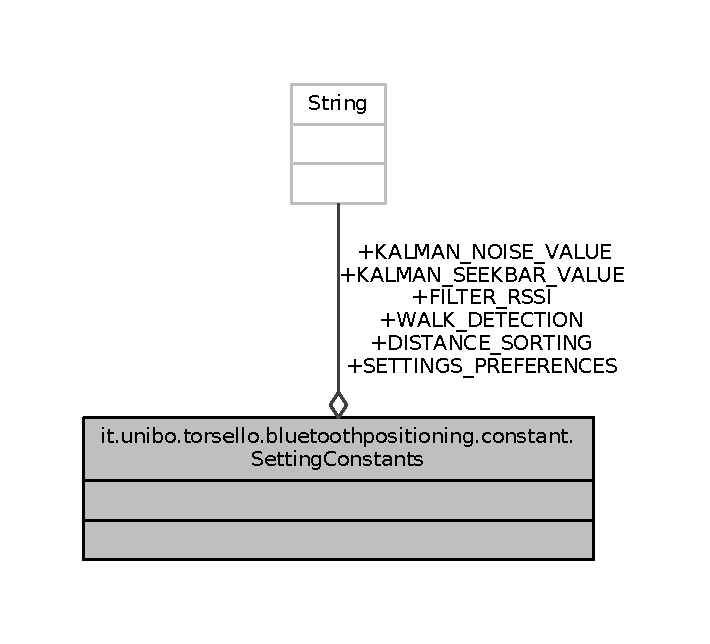
\includegraphics[width=342pt]{classit_1_1unibo_1_1torsello_1_1bluetoothpositioning_1_1constant_1_1SettingConstants__coll__graph}
\end{center}
\end{figure}
\subsubsection*{Attributi pubblici statici}
\begin{DoxyCompactItemize}
\item 
static final String \hyperlink{classit_1_1unibo_1_1torsello_1_1bluetoothpositioning_1_1constant_1_1SettingConstants_ae1b406c787a7efb87d585d5c8b80493d_ae1b406c787a7efb87d585d5c8b80493d}{S\+E\+T\+T\+I\+N\+G\+S\+\_\+\+P\+R\+E\+F\+E\+R\+E\+N\+C\+ES} = \char`\"{}settings\+\_\+preferences\char`\"{}
\item 
static final String \hyperlink{classit_1_1unibo_1_1torsello_1_1bluetoothpositioning_1_1constant_1_1SettingConstants_a60a6d73ab1d42653b8a0c5b10c1c80c5_a60a6d73ab1d42653b8a0c5b10c1c80c5}{F\+I\+L\+T\+E\+R\+\_\+\+R\+S\+SI} = \char`\"{}filter\+\_\+rssi\char`\"{}
\item 
static final String \hyperlink{classit_1_1unibo_1_1torsello_1_1bluetoothpositioning_1_1constant_1_1SettingConstants_ad8f1f7986a4558736769604d606f53a1_ad8f1f7986a4558736769604d606f53a1}{A\+R\+M\+A\+\_\+\+O\+P\+T\+I\+ON} = \char`\"{}arma\+\_\+option\char`\"{}
\item 
static final String \hyperlink{classit_1_1unibo_1_1torsello_1_1bluetoothpositioning_1_1constant_1_1SettingConstants_a2c0b004552568f9813696b26b89b840c_a2c0b004552568f9813696b26b89b840c}{A\+V\+G\+\_\+\+O\+P\+T\+I\+ON} = \char`\"{}avg\+\_\+option\char`\"{}
\item 
static final String \hyperlink{classit_1_1unibo_1_1torsello_1_1bluetoothpositioning_1_1constant_1_1SettingConstants_a7ba43b29e467efb129d86c917734c94b_a7ba43b29e467efb129d86c917734c94b}{K\+A\+L\+M\+A\+N\+\_\+\+S\+E\+E\+K\+B\+A\+R\+\_\+\+V\+A\+L\+UE} = \char`\"{}kalman\+\_\+filter\+\_\+seek\+\_\+value\char`\"{}
\item 
static final String \hyperlink{classit_1_1unibo_1_1torsello_1_1bluetoothpositioning_1_1constant_1_1SettingConstants_a2751989834b974103dda417fb8b10337_a2751989834b974103dda417fb8b10337}{K\+A\+L\+M\+A\+N\+\_\+\+N\+O\+I\+S\+E\+\_\+\+V\+A\+L\+UE} = \char`\"{}kalman\+\_\+filter\+\_\+noise\+\_\+value\char`\"{}
\item 
static final String \hyperlink{classit_1_1unibo_1_1torsello_1_1bluetoothpositioning_1_1constant_1_1SettingConstants_a974ee83a6959f7965c5fa27ac8dc0798_a974ee83a6959f7965c5fa27ac8dc0798}{K\+A\+L\+M\+A\+N\+\_\+\+F\+I\+L\+T\+E\+R\+\_\+\+E\+N\+A\+B\+L\+ED} = \char`\"{}kalma\+\_\+filrer\+\_\+enabled\char`\"{}
\item 
static final String \hyperlink{classit_1_1unibo_1_1torsello_1_1bluetoothpositioning_1_1constant_1_1SettingConstants_ad86af94213ec3f11669289c4972c7658_ad86af94213ec3f11669289c4972c7658}{D\+I\+S\+T\+A\+N\+C\+E\+\_\+\+S\+O\+R\+T\+I\+NG} = \char`\"{}distance\+\_\+sorting\+\_\+selected\char`\"{}
\end{DoxyCompactItemize}


\subsubsection{Descrizione dettagliata}
Created by Federico Torsello. \href{mailto:federico.torsello@studio.unibo.it}{\tt federico.\+torsello@studio.\+unibo.\+it} 

A class containing constants for the Shared\+Preference objects. 

\subsubsection{Documentazione dei membri dato}
\hypertarget{classit_1_1unibo_1_1torsello_1_1bluetoothpositioning_1_1constant_1_1SettingConstants_ad8f1f7986a4558736769604d606f53a1_ad8f1f7986a4558736769604d606f53a1}{}\label{classit_1_1unibo_1_1torsello_1_1bluetoothpositioning_1_1constant_1_1SettingConstants_ad8f1f7986a4558736769604d606f53a1_ad8f1f7986a4558736769604d606f53a1} 
\index{it\+::unibo\+::torsello\+::bluetoothpositioning\+::constant\+::\+Setting\+Constants@{it\+::unibo\+::torsello\+::bluetoothpositioning\+::constant\+::\+Setting\+Constants}!A\+R\+M\+A\+\_\+\+O\+P\+T\+I\+ON@{A\+R\+M\+A\+\_\+\+O\+P\+T\+I\+ON}}
\index{A\+R\+M\+A\+\_\+\+O\+P\+T\+I\+ON@{A\+R\+M\+A\+\_\+\+O\+P\+T\+I\+ON}!it\+::unibo\+::torsello\+::bluetoothpositioning\+::constant\+::\+Setting\+Constants@{it\+::unibo\+::torsello\+::bluetoothpositioning\+::constant\+::\+Setting\+Constants}}
\paragraph{\texorpdfstring{A\+R\+M\+A\+\_\+\+O\+P\+T\+I\+ON}{ARMA\_OPTION}}
{\footnotesize\ttfamily final String it.\+unibo.\+torsello.\+bluetoothpositioning.\+constant.\+Setting\+Constants.\+A\+R\+M\+A\+\_\+\+O\+P\+T\+I\+ON = \char`\"{}arma\+\_\+option\char`\"{}\hspace{0.3cm}{\ttfamily [static]}}

\hypertarget{classit_1_1unibo_1_1torsello_1_1bluetoothpositioning_1_1constant_1_1SettingConstants_a2c0b004552568f9813696b26b89b840c_a2c0b004552568f9813696b26b89b840c}{}\label{classit_1_1unibo_1_1torsello_1_1bluetoothpositioning_1_1constant_1_1SettingConstants_a2c0b004552568f9813696b26b89b840c_a2c0b004552568f9813696b26b89b840c} 
\index{it\+::unibo\+::torsello\+::bluetoothpositioning\+::constant\+::\+Setting\+Constants@{it\+::unibo\+::torsello\+::bluetoothpositioning\+::constant\+::\+Setting\+Constants}!A\+V\+G\+\_\+\+O\+P\+T\+I\+ON@{A\+V\+G\+\_\+\+O\+P\+T\+I\+ON}}
\index{A\+V\+G\+\_\+\+O\+P\+T\+I\+ON@{A\+V\+G\+\_\+\+O\+P\+T\+I\+ON}!it\+::unibo\+::torsello\+::bluetoothpositioning\+::constant\+::\+Setting\+Constants@{it\+::unibo\+::torsello\+::bluetoothpositioning\+::constant\+::\+Setting\+Constants}}
\paragraph{\texorpdfstring{A\+V\+G\+\_\+\+O\+P\+T\+I\+ON}{AVG\_OPTION}}
{\footnotesize\ttfamily final String it.\+unibo.\+torsello.\+bluetoothpositioning.\+constant.\+Setting\+Constants.\+A\+V\+G\+\_\+\+O\+P\+T\+I\+ON = \char`\"{}avg\+\_\+option\char`\"{}\hspace{0.3cm}{\ttfamily [static]}}

\hypertarget{classit_1_1unibo_1_1torsello_1_1bluetoothpositioning_1_1constant_1_1SettingConstants_ad86af94213ec3f11669289c4972c7658_ad86af94213ec3f11669289c4972c7658}{}\label{classit_1_1unibo_1_1torsello_1_1bluetoothpositioning_1_1constant_1_1SettingConstants_ad86af94213ec3f11669289c4972c7658_ad86af94213ec3f11669289c4972c7658} 
\index{it\+::unibo\+::torsello\+::bluetoothpositioning\+::constant\+::\+Setting\+Constants@{it\+::unibo\+::torsello\+::bluetoothpositioning\+::constant\+::\+Setting\+Constants}!D\+I\+S\+T\+A\+N\+C\+E\+\_\+\+S\+O\+R\+T\+I\+NG@{D\+I\+S\+T\+A\+N\+C\+E\+\_\+\+S\+O\+R\+T\+I\+NG}}
\index{D\+I\+S\+T\+A\+N\+C\+E\+\_\+\+S\+O\+R\+T\+I\+NG@{D\+I\+S\+T\+A\+N\+C\+E\+\_\+\+S\+O\+R\+T\+I\+NG}!it\+::unibo\+::torsello\+::bluetoothpositioning\+::constant\+::\+Setting\+Constants@{it\+::unibo\+::torsello\+::bluetoothpositioning\+::constant\+::\+Setting\+Constants}}
\paragraph{\texorpdfstring{D\+I\+S\+T\+A\+N\+C\+E\+\_\+\+S\+O\+R\+T\+I\+NG}{DISTANCE\_SORTING}}
{\footnotesize\ttfamily final String it.\+unibo.\+torsello.\+bluetoothpositioning.\+constant.\+Setting\+Constants.\+D\+I\+S\+T\+A\+N\+C\+E\+\_\+\+S\+O\+R\+T\+I\+NG = \char`\"{}distance\+\_\+sorting\+\_\+selected\char`\"{}\hspace{0.3cm}{\ttfamily [static]}}

\hypertarget{classit_1_1unibo_1_1torsello_1_1bluetoothpositioning_1_1constant_1_1SettingConstants_a60a6d73ab1d42653b8a0c5b10c1c80c5_a60a6d73ab1d42653b8a0c5b10c1c80c5}{}\label{classit_1_1unibo_1_1torsello_1_1bluetoothpositioning_1_1constant_1_1SettingConstants_a60a6d73ab1d42653b8a0c5b10c1c80c5_a60a6d73ab1d42653b8a0c5b10c1c80c5} 
\index{it\+::unibo\+::torsello\+::bluetoothpositioning\+::constant\+::\+Setting\+Constants@{it\+::unibo\+::torsello\+::bluetoothpositioning\+::constant\+::\+Setting\+Constants}!F\+I\+L\+T\+E\+R\+\_\+\+R\+S\+SI@{F\+I\+L\+T\+E\+R\+\_\+\+R\+S\+SI}}
\index{F\+I\+L\+T\+E\+R\+\_\+\+R\+S\+SI@{F\+I\+L\+T\+E\+R\+\_\+\+R\+S\+SI}!it\+::unibo\+::torsello\+::bluetoothpositioning\+::constant\+::\+Setting\+Constants@{it\+::unibo\+::torsello\+::bluetoothpositioning\+::constant\+::\+Setting\+Constants}}
\paragraph{\texorpdfstring{F\+I\+L\+T\+E\+R\+\_\+\+R\+S\+SI}{FILTER\_RSSI}}
{\footnotesize\ttfamily final String it.\+unibo.\+torsello.\+bluetoothpositioning.\+constant.\+Setting\+Constants.\+F\+I\+L\+T\+E\+R\+\_\+\+R\+S\+SI = \char`\"{}filter\+\_\+rssi\char`\"{}\hspace{0.3cm}{\ttfamily [static]}}

\hypertarget{classit_1_1unibo_1_1torsello_1_1bluetoothpositioning_1_1constant_1_1SettingConstants_a974ee83a6959f7965c5fa27ac8dc0798_a974ee83a6959f7965c5fa27ac8dc0798}{}\label{classit_1_1unibo_1_1torsello_1_1bluetoothpositioning_1_1constant_1_1SettingConstants_a974ee83a6959f7965c5fa27ac8dc0798_a974ee83a6959f7965c5fa27ac8dc0798} 
\index{it\+::unibo\+::torsello\+::bluetoothpositioning\+::constant\+::\+Setting\+Constants@{it\+::unibo\+::torsello\+::bluetoothpositioning\+::constant\+::\+Setting\+Constants}!K\+A\+L\+M\+A\+N\+\_\+\+F\+I\+L\+T\+E\+R\+\_\+\+E\+N\+A\+B\+L\+ED@{K\+A\+L\+M\+A\+N\+\_\+\+F\+I\+L\+T\+E\+R\+\_\+\+E\+N\+A\+B\+L\+ED}}
\index{K\+A\+L\+M\+A\+N\+\_\+\+F\+I\+L\+T\+E\+R\+\_\+\+E\+N\+A\+B\+L\+ED@{K\+A\+L\+M\+A\+N\+\_\+\+F\+I\+L\+T\+E\+R\+\_\+\+E\+N\+A\+B\+L\+ED}!it\+::unibo\+::torsello\+::bluetoothpositioning\+::constant\+::\+Setting\+Constants@{it\+::unibo\+::torsello\+::bluetoothpositioning\+::constant\+::\+Setting\+Constants}}
\paragraph{\texorpdfstring{K\+A\+L\+M\+A\+N\+\_\+\+F\+I\+L\+T\+E\+R\+\_\+\+E\+N\+A\+B\+L\+ED}{KALMAN\_FILTER\_ENABLED}}
{\footnotesize\ttfamily final String it.\+unibo.\+torsello.\+bluetoothpositioning.\+constant.\+Setting\+Constants.\+K\+A\+L\+M\+A\+N\+\_\+\+F\+I\+L\+T\+E\+R\+\_\+\+E\+N\+A\+B\+L\+ED = \char`\"{}kalma\+\_\+filrer\+\_\+enabled\char`\"{}\hspace{0.3cm}{\ttfamily [static]}}

\hypertarget{classit_1_1unibo_1_1torsello_1_1bluetoothpositioning_1_1constant_1_1SettingConstants_a2751989834b974103dda417fb8b10337_a2751989834b974103dda417fb8b10337}{}\label{classit_1_1unibo_1_1torsello_1_1bluetoothpositioning_1_1constant_1_1SettingConstants_a2751989834b974103dda417fb8b10337_a2751989834b974103dda417fb8b10337} 
\index{it\+::unibo\+::torsello\+::bluetoothpositioning\+::constant\+::\+Setting\+Constants@{it\+::unibo\+::torsello\+::bluetoothpositioning\+::constant\+::\+Setting\+Constants}!K\+A\+L\+M\+A\+N\+\_\+\+N\+O\+I\+S\+E\+\_\+\+V\+A\+L\+UE@{K\+A\+L\+M\+A\+N\+\_\+\+N\+O\+I\+S\+E\+\_\+\+V\+A\+L\+UE}}
\index{K\+A\+L\+M\+A\+N\+\_\+\+N\+O\+I\+S\+E\+\_\+\+V\+A\+L\+UE@{K\+A\+L\+M\+A\+N\+\_\+\+N\+O\+I\+S\+E\+\_\+\+V\+A\+L\+UE}!it\+::unibo\+::torsello\+::bluetoothpositioning\+::constant\+::\+Setting\+Constants@{it\+::unibo\+::torsello\+::bluetoothpositioning\+::constant\+::\+Setting\+Constants}}
\paragraph{\texorpdfstring{K\+A\+L\+M\+A\+N\+\_\+\+N\+O\+I\+S\+E\+\_\+\+V\+A\+L\+UE}{KALMAN\_NOISE\_VALUE}}
{\footnotesize\ttfamily final String it.\+unibo.\+torsello.\+bluetoothpositioning.\+constant.\+Setting\+Constants.\+K\+A\+L\+M\+A\+N\+\_\+\+N\+O\+I\+S\+E\+\_\+\+V\+A\+L\+UE = \char`\"{}kalman\+\_\+filter\+\_\+noise\+\_\+value\char`\"{}\hspace{0.3cm}{\ttfamily [static]}}

\hypertarget{classit_1_1unibo_1_1torsello_1_1bluetoothpositioning_1_1constant_1_1SettingConstants_a7ba43b29e467efb129d86c917734c94b_a7ba43b29e467efb129d86c917734c94b}{}\label{classit_1_1unibo_1_1torsello_1_1bluetoothpositioning_1_1constant_1_1SettingConstants_a7ba43b29e467efb129d86c917734c94b_a7ba43b29e467efb129d86c917734c94b} 
\index{it\+::unibo\+::torsello\+::bluetoothpositioning\+::constant\+::\+Setting\+Constants@{it\+::unibo\+::torsello\+::bluetoothpositioning\+::constant\+::\+Setting\+Constants}!K\+A\+L\+M\+A\+N\+\_\+\+S\+E\+E\+K\+B\+A\+R\+\_\+\+V\+A\+L\+UE@{K\+A\+L\+M\+A\+N\+\_\+\+S\+E\+E\+K\+B\+A\+R\+\_\+\+V\+A\+L\+UE}}
\index{K\+A\+L\+M\+A\+N\+\_\+\+S\+E\+E\+K\+B\+A\+R\+\_\+\+V\+A\+L\+UE@{K\+A\+L\+M\+A\+N\+\_\+\+S\+E\+E\+K\+B\+A\+R\+\_\+\+V\+A\+L\+UE}!it\+::unibo\+::torsello\+::bluetoothpositioning\+::constant\+::\+Setting\+Constants@{it\+::unibo\+::torsello\+::bluetoothpositioning\+::constant\+::\+Setting\+Constants}}
\paragraph{\texorpdfstring{K\+A\+L\+M\+A\+N\+\_\+\+S\+E\+E\+K\+B\+A\+R\+\_\+\+V\+A\+L\+UE}{KALMAN\_SEEKBAR\_VALUE}}
{\footnotesize\ttfamily final String it.\+unibo.\+torsello.\+bluetoothpositioning.\+constant.\+Setting\+Constants.\+K\+A\+L\+M\+A\+N\+\_\+\+S\+E\+E\+K\+B\+A\+R\+\_\+\+V\+A\+L\+UE = \char`\"{}kalman\+\_\+filter\+\_\+seek\+\_\+value\char`\"{}\hspace{0.3cm}{\ttfamily [static]}}

\hypertarget{classit_1_1unibo_1_1torsello_1_1bluetoothpositioning_1_1constant_1_1SettingConstants_ae1b406c787a7efb87d585d5c8b80493d_ae1b406c787a7efb87d585d5c8b80493d}{}\label{classit_1_1unibo_1_1torsello_1_1bluetoothpositioning_1_1constant_1_1SettingConstants_ae1b406c787a7efb87d585d5c8b80493d_ae1b406c787a7efb87d585d5c8b80493d} 
\index{it\+::unibo\+::torsello\+::bluetoothpositioning\+::constant\+::\+Setting\+Constants@{it\+::unibo\+::torsello\+::bluetoothpositioning\+::constant\+::\+Setting\+Constants}!S\+E\+T\+T\+I\+N\+G\+S\+\_\+\+P\+R\+E\+F\+E\+R\+E\+N\+C\+ES@{S\+E\+T\+T\+I\+N\+G\+S\+\_\+\+P\+R\+E\+F\+E\+R\+E\+N\+C\+ES}}
\index{S\+E\+T\+T\+I\+N\+G\+S\+\_\+\+P\+R\+E\+F\+E\+R\+E\+N\+C\+ES@{S\+E\+T\+T\+I\+N\+G\+S\+\_\+\+P\+R\+E\+F\+E\+R\+E\+N\+C\+ES}!it\+::unibo\+::torsello\+::bluetoothpositioning\+::constant\+::\+Setting\+Constants@{it\+::unibo\+::torsello\+::bluetoothpositioning\+::constant\+::\+Setting\+Constants}}
\paragraph{\texorpdfstring{S\+E\+T\+T\+I\+N\+G\+S\+\_\+\+P\+R\+E\+F\+E\+R\+E\+N\+C\+ES}{SETTINGS\_PREFERENCES}}
{\footnotesize\ttfamily final String it.\+unibo.\+torsello.\+bluetoothpositioning.\+constant.\+Setting\+Constants.\+S\+E\+T\+T\+I\+N\+G\+S\+\_\+\+P\+R\+E\+F\+E\+R\+E\+N\+C\+ES = \char`\"{}settings\+\_\+preferences\char`\"{}\hspace{0.3cm}{\ttfamily [static]}}



La documentazione per questa classe è stata generata a partire dal seguente file\+:\begin{DoxyCompactItemize}
\item 
\hyperlink{SettingConstants_8java}{Setting\+Constants.\+java}\end{DoxyCompactItemize}

\hypertarget{classit_1_1unibo_1_1torsello_1_1bluetoothpositioning_1_1fragment_1_1SettingsFragment}{}\subsection{Riferimenti per la classe it.\+unibo.\+torsello.\+bluetoothpositioning.\+fragment.\+Settings\+Fragment}
\label{classit_1_1unibo_1_1torsello_1_1bluetoothpositioning_1_1fragment_1_1SettingsFragment}\index{it.\+unibo.\+torsello.\+bluetoothpositioning.\+fragment.\+Settings\+Fragment@{it.\+unibo.\+torsello.\+bluetoothpositioning.\+fragment.\+Settings\+Fragment}}


Diagramma delle classi per it.\+unibo.\+torsello.\+bluetoothpositioning.\+fragment.\+Settings\+Fragment
\nopagebreak
\begin{figure}[H]
\begin{center}
\leavevmode
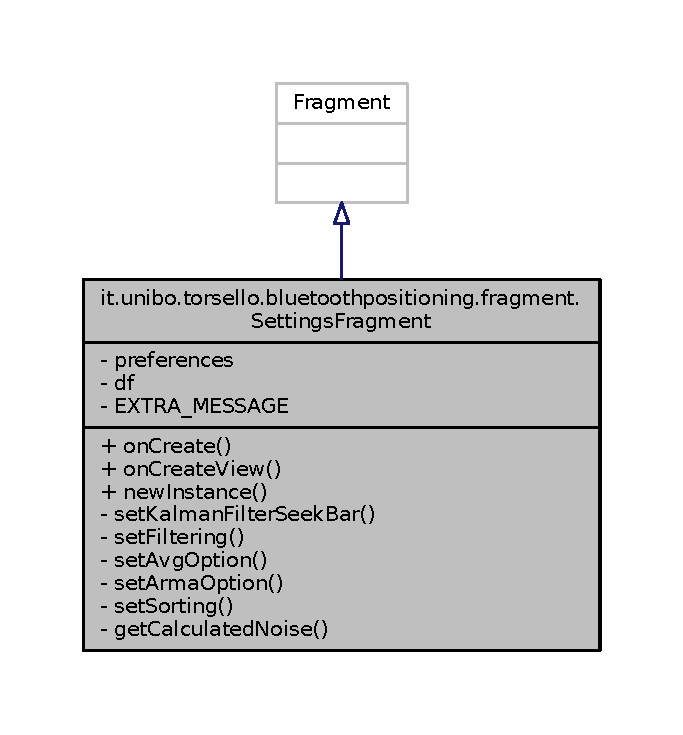
\includegraphics[width=328pt]{classit_1_1unibo_1_1torsello_1_1bluetoothpositioning_1_1fragment_1_1SettingsFragment__inherit__graph}
\end{center}
\end{figure}


Diagramma di collaborazione per it.\+unibo.\+torsello.\+bluetoothpositioning.\+fragment.\+Settings\+Fragment\+:
\nopagebreak
\begin{figure}[H]
\begin{center}
\leavevmode
\includegraphics[width=350pt]{classit_1_1unibo_1_1torsello_1_1bluetoothpositioning_1_1fragment_1_1SettingsFragment__coll__graph}
\end{center}
\end{figure}
\subsubsection*{Membri pubblici}
\begin{DoxyCompactItemize}
\item 
void \hyperlink{classit_1_1unibo_1_1torsello_1_1bluetoothpositioning_1_1fragment_1_1SettingsFragment_a7de90efb25e655078f5f8984f7c6d628_a7de90efb25e655078f5f8984f7c6d628}{on\+Create} (Bundle saved\+Instance\+State)
\item 
View \hyperlink{classit_1_1unibo_1_1torsello_1_1bluetoothpositioning_1_1fragment_1_1SettingsFragment_ac1c9d47777382cc2c74b7b1cf3d6ccd7_ac1c9d47777382cc2c74b7b1cf3d6ccd7}{on\+Create\+View} (Layout\+Inflater inflater, View\+Group container, Bundle saved\+Instance\+State)
\end{DoxyCompactItemize}
\subsubsection*{Membri pubblici statici}
\begin{DoxyCompactItemize}
\item 
static \hyperlink{classit_1_1unibo_1_1torsello_1_1bluetoothpositioning_1_1fragment_1_1SettingsFragment}{Settings\+Fragment} \hyperlink{classit_1_1unibo_1_1torsello_1_1bluetoothpositioning_1_1fragment_1_1SettingsFragment_a4eb69c78cde2ba119eb62453688280f5_a4eb69c78cde2ba119eb62453688280f5}{new\+Instance} ()
\end{DoxyCompactItemize}
\subsubsection*{Membri privati}
\begin{DoxyCompactItemize}
\item 
void \hyperlink{classit_1_1unibo_1_1torsello_1_1bluetoothpositioning_1_1fragment_1_1SettingsFragment_a84057f1633708ec85de5968ed9e7f032_a84057f1633708ec85de5968ed9e7f032}{set\+Kalman\+Filter\+Seek\+Bar} (View root)
\item 
void \hyperlink{classit_1_1unibo_1_1torsello_1_1bluetoothpositioning_1_1fragment_1_1SettingsFragment_ae16c093ba7bc137acf21dfc221cdcf56_ae16c093ba7bc137acf21dfc221cdcf56}{set\+Enabled\+Kalman\+Filter} (int progress)
\item 
void \hyperlink{classit_1_1unibo_1_1torsello_1_1bluetoothpositioning_1_1fragment_1_1SettingsFragment_a0d7b911602439aaf2a9ee4d5f9e41088_a0d7b911602439aaf2a9ee4d5f9e41088}{set\+Filtering} (View root)
\item 
void \hyperlink{classit_1_1unibo_1_1torsello_1_1bluetoothpositioning_1_1fragment_1_1SettingsFragment_a0f26c84f3a3dfffabfed1db04303b8b0_a0f26c84f3a3dfffabfed1db04303b8b0}{set\+Avg\+Option} (View root)
\item 
void \hyperlink{classit_1_1unibo_1_1torsello_1_1bluetoothpositioning_1_1fragment_1_1SettingsFragment_a093ab503fb5dc6ddb859b128b614d902_a093ab503fb5dc6ddb859b128b614d902}{set\+Arma\+Option} (View root)
\item 
void \hyperlink{classit_1_1unibo_1_1torsello_1_1bluetoothpositioning_1_1fragment_1_1SettingsFragment_ae29f0b3d6fc60f1ceeab5dcc530166c1_ae29f0b3d6fc60f1ceeab5dcc530166c1}{set\+Sorting} (View root)
\end{DoxyCompactItemize}
\subsubsection*{Membri privati statici}
\begin{DoxyCompactItemize}
\item 
static float \hyperlink{classit_1_1unibo_1_1torsello_1_1bluetoothpositioning_1_1fragment_1_1SettingsFragment_a595d859602f34ca81957a0578c1602a6_a595d859602f34ca81957a0578c1602a6}{get\+Calculated\+Noise} (int p)
\end{DoxyCompactItemize}
\subsubsection*{Attributi privati}
\begin{DoxyCompactItemize}
\item 
Shared\+Preferences \hyperlink{classit_1_1unibo_1_1torsello_1_1bluetoothpositioning_1_1fragment_1_1SettingsFragment_a52480c4d5d81ca59fe4a98ae3c623ea4_a52480c4d5d81ca59fe4a98ae3c623ea4}{preferences}
\item 
Decimal\+Format \hyperlink{classit_1_1unibo_1_1torsello_1_1bluetoothpositioning_1_1fragment_1_1SettingsFragment_af6b80a700dc80c39a56d001b68a47694_af6b80a700dc80c39a56d001b68a47694}{df}
\end{DoxyCompactItemize}
\subsubsection*{Attributi privati statici}
\begin{DoxyCompactItemize}
\item 
static final String \hyperlink{classit_1_1unibo_1_1torsello_1_1bluetoothpositioning_1_1fragment_1_1SettingsFragment_a3f3c627008cd1e176afc52642c73fd93_a3f3c627008cd1e176afc52642c73fd93}{E\+X\+T\+R\+A\+\_\+\+M\+E\+S\+S\+A\+GE} = \char`\"{}E\+X\+T\+R\+A\+\_\+\+M\+E\+S\+S\+A\+GE\char`\"{}
\end{DoxyCompactItemize}


\subsubsection{Descrizione dettagliata}
Created by Federico Torsello. \href{mailto:federico.torsello@studio.unibo.it}{\tt federico.\+torsello@studio.\+unibo.\+it} 

\subsubsection{Documentazione delle funzioni membro}
\hypertarget{classit_1_1unibo_1_1torsello_1_1bluetoothpositioning_1_1fragment_1_1SettingsFragment_a595d859602f34ca81957a0578c1602a6_a595d859602f34ca81957a0578c1602a6}{}\label{classit_1_1unibo_1_1torsello_1_1bluetoothpositioning_1_1fragment_1_1SettingsFragment_a595d859602f34ca81957a0578c1602a6_a595d859602f34ca81957a0578c1602a6} 
\index{it\+::unibo\+::torsello\+::bluetoothpositioning\+::fragment\+::\+Settings\+Fragment@{it\+::unibo\+::torsello\+::bluetoothpositioning\+::fragment\+::\+Settings\+Fragment}!get\+Calculated\+Noise@{get\+Calculated\+Noise}}
\index{get\+Calculated\+Noise@{get\+Calculated\+Noise}!it\+::unibo\+::torsello\+::bluetoothpositioning\+::fragment\+::\+Settings\+Fragment@{it\+::unibo\+::torsello\+::bluetoothpositioning\+::fragment\+::\+Settings\+Fragment}}
\paragraph{\texorpdfstring{get\+Calculated\+Noise()}{getCalculatedNoise()}}
{\footnotesize\ttfamily static float it.\+unibo.\+torsello.\+bluetoothpositioning.\+fragment.\+Settings\+Fragment.\+get\+Calculated\+Noise (\begin{DoxyParamCaption}\item[{int}]{p }\end{DoxyParamCaption})\hspace{0.3cm}{\ttfamily [static]}, {\ttfamily [private]}}


\begin{DoxyCode}
112                                                    \{
113         \textcolor{keywordtype}{double} percent = (p / 10D);
114         \textcolor{keywordtype}{double} noise = KFilterConstants.KALMAN\_NOISE\_MIN +
115                 (KFilterConstants.KALMAN\_NOISE\_MAX - KFilterConstants.KALMAN\_NOISE\_MIN) * percent;
116 
117         \textcolor{keywordflow}{return} (\textcolor{keywordtype}{float}) noise;
118 
119     \}
\end{DoxyCode}
\hypertarget{classit_1_1unibo_1_1torsello_1_1bluetoothpositioning_1_1fragment_1_1SettingsFragment_a4eb69c78cde2ba119eb62453688280f5_a4eb69c78cde2ba119eb62453688280f5}{}\label{classit_1_1unibo_1_1torsello_1_1bluetoothpositioning_1_1fragment_1_1SettingsFragment_a4eb69c78cde2ba119eb62453688280f5_a4eb69c78cde2ba119eb62453688280f5} 
\index{it\+::unibo\+::torsello\+::bluetoothpositioning\+::fragment\+::\+Settings\+Fragment@{it\+::unibo\+::torsello\+::bluetoothpositioning\+::fragment\+::\+Settings\+Fragment}!new\+Instance@{new\+Instance}}
\index{new\+Instance@{new\+Instance}!it\+::unibo\+::torsello\+::bluetoothpositioning\+::fragment\+::\+Settings\+Fragment@{it\+::unibo\+::torsello\+::bluetoothpositioning\+::fragment\+::\+Settings\+Fragment}}
\paragraph{\texorpdfstring{new\+Instance()}{newInstance()}}
{\footnotesize\ttfamily static \hyperlink{classit_1_1unibo_1_1torsello_1_1bluetoothpositioning_1_1fragment_1_1SettingsFragment}{Settings\+Fragment} it.\+unibo.\+torsello.\+bluetoothpositioning.\+fragment.\+Settings\+Fragment.\+new\+Instance (\begin{DoxyParamCaption}{ }\end{DoxyParamCaption})\hspace{0.3cm}{\ttfamily [static]}}


\begin{DoxyCode}
29                                                  \{
30         SettingsFragment fragment = \textcolor{keyword}{new} SettingsFragment();
31         Bundle args = \textcolor{keyword}{new} Bundle();
32         args.putString(\hyperlink{classit_1_1unibo_1_1torsello_1_1bluetoothpositioning_1_1fragment_1_1SettingsFragment_a3f3c627008cd1e176afc52642c73fd93_a3f3c627008cd1e176afc52642c73fd93}{EXTRA\_MESSAGE}, \textcolor{stringliteral}{"Settings"});
33         fragment.setArguments(args);
34         \textcolor{keywordflow}{return} fragment;
35     \}
\end{DoxyCode}
\hypertarget{classit_1_1unibo_1_1torsello_1_1bluetoothpositioning_1_1fragment_1_1SettingsFragment_a7de90efb25e655078f5f8984f7c6d628_a7de90efb25e655078f5f8984f7c6d628}{}\label{classit_1_1unibo_1_1torsello_1_1bluetoothpositioning_1_1fragment_1_1SettingsFragment_a7de90efb25e655078f5f8984f7c6d628_a7de90efb25e655078f5f8984f7c6d628} 
\index{it\+::unibo\+::torsello\+::bluetoothpositioning\+::fragment\+::\+Settings\+Fragment@{it\+::unibo\+::torsello\+::bluetoothpositioning\+::fragment\+::\+Settings\+Fragment}!on\+Create@{on\+Create}}
\index{on\+Create@{on\+Create}!it\+::unibo\+::torsello\+::bluetoothpositioning\+::fragment\+::\+Settings\+Fragment@{it\+::unibo\+::torsello\+::bluetoothpositioning\+::fragment\+::\+Settings\+Fragment}}
\paragraph{\texorpdfstring{on\+Create()}{onCreate()}}
{\footnotesize\ttfamily void it.\+unibo.\+torsello.\+bluetoothpositioning.\+fragment.\+Settings\+Fragment.\+on\+Create (\begin{DoxyParamCaption}\item[{Bundle}]{saved\+Instance\+State }\end{DoxyParamCaption})}


\begin{DoxyCode}
38                                                     \{
39         super.onCreate(savedInstanceState);
40 
41         \hyperlink{classit_1_1unibo_1_1torsello_1_1bluetoothpositioning_1_1fragment_1_1SettingsFragment_a52480c4d5d81ca59fe4a98ae3c623ea4_a52480c4d5d81ca59fe4a98ae3c623ea4}{preferences} = getActivity().getSharedPreferences(SettingConstants.SETTINGS\_PREFERENCES, 
      0);
42         \hyperlink{classit_1_1unibo_1_1torsello_1_1bluetoothpositioning_1_1fragment_1_1SettingsFragment_af6b80a700dc80c39a56d001b68a47694_af6b80a700dc80c39a56d001b68a47694}{df} = \textcolor{keyword}{new} DecimalFormat(\textcolor{stringliteral}{"0.0#"});
43     \}
\end{DoxyCode}
\hypertarget{classit_1_1unibo_1_1torsello_1_1bluetoothpositioning_1_1fragment_1_1SettingsFragment_ac1c9d47777382cc2c74b7b1cf3d6ccd7_ac1c9d47777382cc2c74b7b1cf3d6ccd7}{}\label{classit_1_1unibo_1_1torsello_1_1bluetoothpositioning_1_1fragment_1_1SettingsFragment_ac1c9d47777382cc2c74b7b1cf3d6ccd7_ac1c9d47777382cc2c74b7b1cf3d6ccd7} 
\index{it\+::unibo\+::torsello\+::bluetoothpositioning\+::fragment\+::\+Settings\+Fragment@{it\+::unibo\+::torsello\+::bluetoothpositioning\+::fragment\+::\+Settings\+Fragment}!on\+Create\+View@{on\+Create\+View}}
\index{on\+Create\+View@{on\+Create\+View}!it\+::unibo\+::torsello\+::bluetoothpositioning\+::fragment\+::\+Settings\+Fragment@{it\+::unibo\+::torsello\+::bluetoothpositioning\+::fragment\+::\+Settings\+Fragment}}
\paragraph{\texorpdfstring{on\+Create\+View()}{onCreateView()}}
{\footnotesize\ttfamily View it.\+unibo.\+torsello.\+bluetoothpositioning.\+fragment.\+Settings\+Fragment.\+on\+Create\+View (\begin{DoxyParamCaption}\item[{Layout\+Inflater}]{inflater,  }\item[{View\+Group}]{container,  }\item[{Bundle}]{saved\+Instance\+State }\end{DoxyParamCaption})}


\begin{DoxyCode}
46                                                                                                       \{
47         View root = inflater.inflate(R.layout.fragment\_settings, container, \textcolor{keyword}{false});
48 
49         \hyperlink{classit_1_1unibo_1_1torsello_1_1bluetoothpositioning_1_1fragment_1_1SettingsFragment_a84057f1633708ec85de5968ed9e7f032_a84057f1633708ec85de5968ed9e7f032}{setKalmanFilterSeekBar}(root);
50 
51         \hyperlink{classit_1_1unibo_1_1torsello_1_1bluetoothpositioning_1_1fragment_1_1SettingsFragment_a0d7b911602439aaf2a9ee4d5f9e41088_a0d7b911602439aaf2a9ee4d5f9e41088}{setFiltering}(root);
52 
53         \hyperlink{classit_1_1unibo_1_1torsello_1_1bluetoothpositioning_1_1fragment_1_1SettingsFragment_a093ab503fb5dc6ddb859b128b614d902_a093ab503fb5dc6ddb859b128b614d902}{setArmaOption}(root);
54 
55         \hyperlink{classit_1_1unibo_1_1torsello_1_1bluetoothpositioning_1_1fragment_1_1SettingsFragment_a0f26c84f3a3dfffabfed1db04303b8b0_a0f26c84f3a3dfffabfed1db04303b8b0}{setAvgOption}(root);
56 
57         \hyperlink{classit_1_1unibo_1_1torsello_1_1bluetoothpositioning_1_1fragment_1_1SettingsFragment_ae29f0b3d6fc60f1ceeab5dcc530166c1_ae29f0b3d6fc60f1ceeab5dcc530166c1}{setSorting}(root);
58 
59         \textcolor{keywordflow}{return} root;
60     \}
\end{DoxyCode}
\hypertarget{classit_1_1unibo_1_1torsello_1_1bluetoothpositioning_1_1fragment_1_1SettingsFragment_a093ab503fb5dc6ddb859b128b614d902_a093ab503fb5dc6ddb859b128b614d902}{}\label{classit_1_1unibo_1_1torsello_1_1bluetoothpositioning_1_1fragment_1_1SettingsFragment_a093ab503fb5dc6ddb859b128b614d902_a093ab503fb5dc6ddb859b128b614d902} 
\index{it\+::unibo\+::torsello\+::bluetoothpositioning\+::fragment\+::\+Settings\+Fragment@{it\+::unibo\+::torsello\+::bluetoothpositioning\+::fragment\+::\+Settings\+Fragment}!set\+Arma\+Option@{set\+Arma\+Option}}
\index{set\+Arma\+Option@{set\+Arma\+Option}!it\+::unibo\+::torsello\+::bluetoothpositioning\+::fragment\+::\+Settings\+Fragment@{it\+::unibo\+::torsello\+::bluetoothpositioning\+::fragment\+::\+Settings\+Fragment}}
\paragraph{\texorpdfstring{set\+Arma\+Option()}{setArmaOption()}}
{\footnotesize\ttfamily void it.\+unibo.\+torsello.\+bluetoothpositioning.\+fragment.\+Settings\+Fragment.\+set\+Arma\+Option (\begin{DoxyParamCaption}\item[{View}]{root }\end{DoxyParamCaption})\hspace{0.3cm}{\ttfamily [private]}}


\begin{DoxyCode}
159                                           \{
160         RadioGroup rg = (RadioGroup) root.findViewById(R.id.radioGroupArmaOptions);
161         \textcolor{keywordtype}{int} checkedRadioButton;
162         \textcolor{keywordflow}{if} (rg.getCheckedRadioButtonId() != 0) \{
163             checkedRadioButton = \hyperlink{classit_1_1unibo_1_1torsello_1_1bluetoothpositioning_1_1fragment_1_1SettingsFragment_a52480c4d5d81ca59fe4a98ae3c623ea4_a52480c4d5d81ca59fe4a98ae3c623ea4}{preferences}.getInt(SettingConstants.ARMA\_OPTION, rg.
      getCheckedRadioButtonId());
164         \} \textcolor{keywordflow}{else} \{
165             checkedRadioButton = 0;
166         \}
167         rg.check(checkedRadioButton);
168         rg.setOnCheckedChangeListener(\textcolor{keyword}{new} RadioGroup.OnCheckedChangeListener() \{
169             @Override
170             \textcolor{keyword}{public} \textcolor{keywordtype}{void} onCheckedChanged(RadioGroup group, \textcolor{keywordtype}{int} checkedId) \{
171                 SharedPreferences.Editor editor = \hyperlink{classit_1_1unibo_1_1torsello_1_1bluetoothpositioning_1_1fragment_1_1SettingsFragment_a52480c4d5d81ca59fe4a98ae3c623ea4_a52480c4d5d81ca59fe4a98ae3c623ea4}{preferences}.edit();
172                 editor.putInt(SettingConstants.ARMA\_OPTION, checkedId);
173                 editor.apply();
174             \}
175         \});
176     \}
\end{DoxyCode}
\hypertarget{classit_1_1unibo_1_1torsello_1_1bluetoothpositioning_1_1fragment_1_1SettingsFragment_a0f26c84f3a3dfffabfed1db04303b8b0_a0f26c84f3a3dfffabfed1db04303b8b0}{}\label{classit_1_1unibo_1_1torsello_1_1bluetoothpositioning_1_1fragment_1_1SettingsFragment_a0f26c84f3a3dfffabfed1db04303b8b0_a0f26c84f3a3dfffabfed1db04303b8b0} 
\index{it\+::unibo\+::torsello\+::bluetoothpositioning\+::fragment\+::\+Settings\+Fragment@{it\+::unibo\+::torsello\+::bluetoothpositioning\+::fragment\+::\+Settings\+Fragment}!set\+Avg\+Option@{set\+Avg\+Option}}
\index{set\+Avg\+Option@{set\+Avg\+Option}!it\+::unibo\+::torsello\+::bluetoothpositioning\+::fragment\+::\+Settings\+Fragment@{it\+::unibo\+::torsello\+::bluetoothpositioning\+::fragment\+::\+Settings\+Fragment}}
\paragraph{\texorpdfstring{set\+Avg\+Option()}{setAvgOption()}}
{\footnotesize\ttfamily void it.\+unibo.\+torsello.\+bluetoothpositioning.\+fragment.\+Settings\+Fragment.\+set\+Avg\+Option (\begin{DoxyParamCaption}\item[{View}]{root }\end{DoxyParamCaption})\hspace{0.3cm}{\ttfamily [private]}}


\begin{DoxyCode}
140                                          \{
141         RadioGroup rg = (RadioGroup) root.findViewById(R.id.radioGroupAverageOptions);
142         \textcolor{keywordtype}{int} checkedRadioButton;
143         \textcolor{keywordflow}{if} (rg.getCheckedRadioButtonId() != 0) \{
144             checkedRadioButton = \hyperlink{classit_1_1unibo_1_1torsello_1_1bluetoothpositioning_1_1fragment_1_1SettingsFragment_a52480c4d5d81ca59fe4a98ae3c623ea4_a52480c4d5d81ca59fe4a98ae3c623ea4}{preferences}.getInt(SettingConstants.AVG\_OPTION, rg.
      getCheckedRadioButtonId());
145         \} \textcolor{keywordflow}{else} \{
146             checkedRadioButton = 0;
147         \}
148         rg.check(checkedRadioButton);
149         rg.setOnCheckedChangeListener(\textcolor{keyword}{new} RadioGroup.OnCheckedChangeListener() \{
150             @Override
151             \textcolor{keyword}{public} \textcolor{keywordtype}{void} onCheckedChanged(RadioGroup group, \textcolor{keywordtype}{int} checkedId) \{
152                 SharedPreferences.Editor editor = \hyperlink{classit_1_1unibo_1_1torsello_1_1bluetoothpositioning_1_1fragment_1_1SettingsFragment_a52480c4d5d81ca59fe4a98ae3c623ea4_a52480c4d5d81ca59fe4a98ae3c623ea4}{preferences}.edit();
153                 editor.putInt(SettingConstants.AVG\_OPTION, checkedId);
154                 editor.apply();
155             \}
156         \});
157     \}
\end{DoxyCode}
\hypertarget{classit_1_1unibo_1_1torsello_1_1bluetoothpositioning_1_1fragment_1_1SettingsFragment_ae16c093ba7bc137acf21dfc221cdcf56_ae16c093ba7bc137acf21dfc221cdcf56}{}\label{classit_1_1unibo_1_1torsello_1_1bluetoothpositioning_1_1fragment_1_1SettingsFragment_ae16c093ba7bc137acf21dfc221cdcf56_ae16c093ba7bc137acf21dfc221cdcf56} 
\index{it\+::unibo\+::torsello\+::bluetoothpositioning\+::fragment\+::\+Settings\+Fragment@{it\+::unibo\+::torsello\+::bluetoothpositioning\+::fragment\+::\+Settings\+Fragment}!set\+Enabled\+Kalman\+Filter@{set\+Enabled\+Kalman\+Filter}}
\index{set\+Enabled\+Kalman\+Filter@{set\+Enabled\+Kalman\+Filter}!it\+::unibo\+::torsello\+::bluetoothpositioning\+::fragment\+::\+Settings\+Fragment@{it\+::unibo\+::torsello\+::bluetoothpositioning\+::fragment\+::\+Settings\+Fragment}}
\paragraph{\texorpdfstring{set\+Enabled\+Kalman\+Filter()}{setEnabledKalmanFilter()}}
{\footnotesize\ttfamily void it.\+unibo.\+torsello.\+bluetoothpositioning.\+fragment.\+Settings\+Fragment.\+set\+Enabled\+Kalman\+Filter (\begin{DoxyParamCaption}\item[{int}]{progress }\end{DoxyParamCaption})\hspace{0.3cm}{\ttfamily [private]}}


\begin{DoxyCode}
101                                                       \{
102         SharedPreferences.Editor editor = \hyperlink{classit_1_1unibo_1_1torsello_1_1bluetoothpositioning_1_1fragment_1_1SettingsFragment_a52480c4d5d81ca59fe4a98ae3c623ea4_a52480c4d5d81ca59fe4a98ae3c623ea4}{preferences}.edit();
103 
104         \textcolor{keywordflow}{if} (progress > 0) \{
105             editor.putBoolean(SettingConstants.KALMAN\_FILTER\_ENABLED, \textcolor{keyword}{true});
106         \} \textcolor{keywordflow}{else} \{
107             editor.putBoolean(SettingConstants.KALMAN\_FILTER\_ENABLED, \textcolor{keyword}{false});
108         \}
109         editor.apply();
110     \}
\end{DoxyCode}
\hypertarget{classit_1_1unibo_1_1torsello_1_1bluetoothpositioning_1_1fragment_1_1SettingsFragment_a0d7b911602439aaf2a9ee4d5f9e41088_a0d7b911602439aaf2a9ee4d5f9e41088}{}\label{classit_1_1unibo_1_1torsello_1_1bluetoothpositioning_1_1fragment_1_1SettingsFragment_a0d7b911602439aaf2a9ee4d5f9e41088_a0d7b911602439aaf2a9ee4d5f9e41088} 
\index{it\+::unibo\+::torsello\+::bluetoothpositioning\+::fragment\+::\+Settings\+Fragment@{it\+::unibo\+::torsello\+::bluetoothpositioning\+::fragment\+::\+Settings\+Fragment}!set\+Filtering@{set\+Filtering}}
\index{set\+Filtering@{set\+Filtering}!it\+::unibo\+::torsello\+::bluetoothpositioning\+::fragment\+::\+Settings\+Fragment@{it\+::unibo\+::torsello\+::bluetoothpositioning\+::fragment\+::\+Settings\+Fragment}}
\paragraph{\texorpdfstring{set\+Filtering()}{setFiltering()}}
{\footnotesize\ttfamily void it.\+unibo.\+torsello.\+bluetoothpositioning.\+fragment.\+Settings\+Fragment.\+set\+Filtering (\begin{DoxyParamCaption}\item[{View}]{root }\end{DoxyParamCaption})\hspace{0.3cm}{\ttfamily [private]}}


\begin{DoxyCode}
121                                          \{
122         RadioGroup rg = (RadioGroup) root.findViewById(R.id.radioGroupFilter);
123         \textcolor{keywordtype}{int} checkedRadioButton;
124         \textcolor{keywordflow}{if} (rg.getCheckedRadioButtonId() != 0) \{
125             checkedRadioButton = \hyperlink{classit_1_1unibo_1_1torsello_1_1bluetoothpositioning_1_1fragment_1_1SettingsFragment_a52480c4d5d81ca59fe4a98ae3c623ea4_a52480c4d5d81ca59fe4a98ae3c623ea4}{preferences}.getInt(SettingConstants.FILTER\_RSSI, rg.
      getCheckedRadioButtonId());
126         \} \textcolor{keywordflow}{else} \{
127             checkedRadioButton = 0;
128         \}
129         rg.check(checkedRadioButton);
130         rg.setOnCheckedChangeListener(\textcolor{keyword}{new} RadioGroup.OnCheckedChangeListener() \{
131             @Override
132             \textcolor{keyword}{public} \textcolor{keywordtype}{void} onCheckedChanged(RadioGroup group, \textcolor{keywordtype}{int} checkedId) \{
133                 SharedPreferences.Editor editor = \hyperlink{classit_1_1unibo_1_1torsello_1_1bluetoothpositioning_1_1fragment_1_1SettingsFragment_a52480c4d5d81ca59fe4a98ae3c623ea4_a52480c4d5d81ca59fe4a98ae3c623ea4}{preferences}.edit();
134                 editor.putInt(SettingConstants.FILTER\_RSSI, checkedId);
135                 editor.apply();
136             \}
137         \});
138     \}
\end{DoxyCode}
\hypertarget{classit_1_1unibo_1_1torsello_1_1bluetoothpositioning_1_1fragment_1_1SettingsFragment_a84057f1633708ec85de5968ed9e7f032_a84057f1633708ec85de5968ed9e7f032}{}\label{classit_1_1unibo_1_1torsello_1_1bluetoothpositioning_1_1fragment_1_1SettingsFragment_a84057f1633708ec85de5968ed9e7f032_a84057f1633708ec85de5968ed9e7f032} 
\index{it\+::unibo\+::torsello\+::bluetoothpositioning\+::fragment\+::\+Settings\+Fragment@{it\+::unibo\+::torsello\+::bluetoothpositioning\+::fragment\+::\+Settings\+Fragment}!set\+Kalman\+Filter\+Seek\+Bar@{set\+Kalman\+Filter\+Seek\+Bar}}
\index{set\+Kalman\+Filter\+Seek\+Bar@{set\+Kalman\+Filter\+Seek\+Bar}!it\+::unibo\+::torsello\+::bluetoothpositioning\+::fragment\+::\+Settings\+Fragment@{it\+::unibo\+::torsello\+::bluetoothpositioning\+::fragment\+::\+Settings\+Fragment}}
\paragraph{\texorpdfstring{set\+Kalman\+Filter\+Seek\+Bar()}{setKalmanFilterSeekBar()}}
{\footnotesize\ttfamily void it.\+unibo.\+torsello.\+bluetoothpositioning.\+fragment.\+Settings\+Fragment.\+set\+Kalman\+Filter\+Seek\+Bar (\begin{DoxyParamCaption}\item[{View}]{root }\end{DoxyParamCaption})\hspace{0.3cm}{\ttfamily [private]}}


\begin{DoxyCode}
63                                                    \{
64         SeekBar kalmanSeek = (SeekBar) root.findViewById(R.id.kalmanSeek);
65         \textcolor{keywordtype}{int} seekValue = \hyperlink{classit_1_1unibo_1_1torsello_1_1bluetoothpositioning_1_1fragment_1_1SettingsFragment_a52480c4d5d81ca59fe4a98ae3c623ea4_a52480c4d5d81ca59fe4a98ae3c623ea4}{preferences}.getInt(SettingConstants.KALMAN\_SEEKBAR\_VALUE, 1);
66 
67         \hyperlink{classit_1_1unibo_1_1torsello_1_1bluetoothpositioning_1_1fragment_1_1SettingsFragment_ae16c093ba7bc137acf21dfc221cdcf56_ae16c093ba7bc137acf21dfc221cdcf56}{setEnabledKalmanFilter}(seekValue);
68 
69         kalmanSeek.setProgress(seekValue);
70 
71         \textcolor{keyword}{final} TextView kalmanFilterValue = (TextView) root.findViewById(R.id.kalmanValue);
72         kalmanFilterValue.setText(\hyperlink{classit_1_1unibo_1_1torsello_1_1bluetoothpositioning_1_1fragment_1_1SettingsFragment_af6b80a700dc80c39a56d001b68a47694_af6b80a700dc80c39a56d001b68a47694}{df}.format(\hyperlink{classit_1_1unibo_1_1torsello_1_1bluetoothpositioning_1_1fragment_1_1SettingsFragment_a595d859602f34ca81957a0578c1602a6_a595d859602f34ca81957a0578c1602a6}{getCalculatedNoise}(seekValue)));
73 
74         kalmanSeek.setOnSeekBarChangeListener(\textcolor{keyword}{new} SeekBar.OnSeekBarChangeListener() \{
75             @Override
76             \textcolor{keyword}{public} \textcolor{keywordtype}{void} onProgressChanged(SeekBar seekBar, \textcolor{keywordtype}{int} seekValue, \textcolor{keywordtype}{boolean} fromUser) \{
77                 kalmanFilterValue.setText(\hyperlink{classit_1_1unibo_1_1torsello_1_1bluetoothpositioning_1_1fragment_1_1SettingsFragment_af6b80a700dc80c39a56d001b68a47694_af6b80a700dc80c39a56d001b68a47694}{df}.format(\hyperlink{classit_1_1unibo_1_1torsello_1_1bluetoothpositioning_1_1fragment_1_1SettingsFragment_a595d859602f34ca81957a0578c1602a6_a595d859602f34ca81957a0578c1602a6}{getCalculatedNoise}(seekValue)));
78             \}
79 
80             @Override
81             \textcolor{keyword}{public} \textcolor{keywordtype}{void} onStartTrackingTouch(SeekBar seekBar) \{
82             \}
83 
84             @Override
85             \textcolor{keyword}{public} \textcolor{keywordtype}{void} onStopTrackingTouch(SeekBar seekBar) \{
86                 SharedPreferences.Editor editor = \hyperlink{classit_1_1unibo_1_1torsello_1_1bluetoothpositioning_1_1fragment_1_1SettingsFragment_a52480c4d5d81ca59fe4a98ae3c623ea4_a52480c4d5d81ca59fe4a98ae3c623ea4}{preferences}.edit();
87 
88                 \textcolor{keywordtype}{int} progress = seekBar.getProgress();
89 
90                 \textcolor{keywordtype}{float} storeProgress = \hyperlink{classit_1_1unibo_1_1torsello_1_1bluetoothpositioning_1_1fragment_1_1SettingsFragment_a595d859602f34ca81957a0578c1602a6_a595d859602f34ca81957a0578c1602a6}{getCalculatedNoise}(progress);
91                 editor.putInt(SettingConstants.KALMAN\_SEEKBAR\_VALUE, progress);
92                 editor.putFloat(SettingConstants.KALMAN\_NOISE\_VALUE, storeProgress);
93                 editor.apply();
94 
95                 \hyperlink{classit_1_1unibo_1_1torsello_1_1bluetoothpositioning_1_1fragment_1_1SettingsFragment_ae16c093ba7bc137acf21dfc221cdcf56_ae16c093ba7bc137acf21dfc221cdcf56}{setEnabledKalmanFilter}(progress);
96                 kalmanFilterValue.setText(\hyperlink{classit_1_1unibo_1_1torsello_1_1bluetoothpositioning_1_1fragment_1_1SettingsFragment_af6b80a700dc80c39a56d001b68a47694_af6b80a700dc80c39a56d001b68a47694}{df}.format(storeProgress));
97             \}
98         \});
99     \}
\end{DoxyCode}
\hypertarget{classit_1_1unibo_1_1torsello_1_1bluetoothpositioning_1_1fragment_1_1SettingsFragment_ae29f0b3d6fc60f1ceeab5dcc530166c1_ae29f0b3d6fc60f1ceeab5dcc530166c1}{}\label{classit_1_1unibo_1_1torsello_1_1bluetoothpositioning_1_1fragment_1_1SettingsFragment_ae29f0b3d6fc60f1ceeab5dcc530166c1_ae29f0b3d6fc60f1ceeab5dcc530166c1} 
\index{it\+::unibo\+::torsello\+::bluetoothpositioning\+::fragment\+::\+Settings\+Fragment@{it\+::unibo\+::torsello\+::bluetoothpositioning\+::fragment\+::\+Settings\+Fragment}!set\+Sorting@{set\+Sorting}}
\index{set\+Sorting@{set\+Sorting}!it\+::unibo\+::torsello\+::bluetoothpositioning\+::fragment\+::\+Settings\+Fragment@{it\+::unibo\+::torsello\+::bluetoothpositioning\+::fragment\+::\+Settings\+Fragment}}
\paragraph{\texorpdfstring{set\+Sorting()}{setSorting()}}
{\footnotesize\ttfamily void it.\+unibo.\+torsello.\+bluetoothpositioning.\+fragment.\+Settings\+Fragment.\+set\+Sorting (\begin{DoxyParamCaption}\item[{View}]{root }\end{DoxyParamCaption})\hspace{0.3cm}{\ttfamily [private]}}


\begin{DoxyCode}
178                                        \{
179         RadioGroup rg = (RadioGroup) root.findViewById(R.id.radioGroupSortingMode);
180         \textcolor{keywordtype}{int} checkedRadioButton;
181         \textcolor{keywordflow}{if} (rg.getCheckedRadioButtonId() != 0) \{
182             checkedRadioButton = \hyperlink{classit_1_1unibo_1_1torsello_1_1bluetoothpositioning_1_1fragment_1_1SettingsFragment_a52480c4d5d81ca59fe4a98ae3c623ea4_a52480c4d5d81ca59fe4a98ae3c623ea4}{preferences}.getInt(SettingConstants.DISTANCE\_SORTING, rg.
      getCheckedRadioButtonId());
183         \} \textcolor{keywordflow}{else} \{
184             checkedRadioButton = 0;
185         \}
186         rg.check(checkedRadioButton);
187         rg.setOnCheckedChangeListener(\textcolor{keyword}{new} RadioGroup.OnCheckedChangeListener() \{
188             @Override
189             \textcolor{keyword}{public} \textcolor{keywordtype}{void} onCheckedChanged(RadioGroup group, \textcolor{keywordtype}{int} checkedId) \{
190                 SharedPreferences.Editor editor = \hyperlink{classit_1_1unibo_1_1torsello_1_1bluetoothpositioning_1_1fragment_1_1SettingsFragment_a52480c4d5d81ca59fe4a98ae3c623ea4_a52480c4d5d81ca59fe4a98ae3c623ea4}{preferences}.edit();
191                 editor.putInt(SettingConstants.DISTANCE\_SORTING, checkedId);
192                 editor.apply();
193             \}
194         \});
195     \}
\end{DoxyCode}


\subsubsection{Documentazione dei membri dato}
\hypertarget{classit_1_1unibo_1_1torsello_1_1bluetoothpositioning_1_1fragment_1_1SettingsFragment_af6b80a700dc80c39a56d001b68a47694_af6b80a700dc80c39a56d001b68a47694}{}\label{classit_1_1unibo_1_1torsello_1_1bluetoothpositioning_1_1fragment_1_1SettingsFragment_af6b80a700dc80c39a56d001b68a47694_af6b80a700dc80c39a56d001b68a47694} 
\index{it\+::unibo\+::torsello\+::bluetoothpositioning\+::fragment\+::\+Settings\+Fragment@{it\+::unibo\+::torsello\+::bluetoothpositioning\+::fragment\+::\+Settings\+Fragment}!df@{df}}
\index{df@{df}!it\+::unibo\+::torsello\+::bluetoothpositioning\+::fragment\+::\+Settings\+Fragment@{it\+::unibo\+::torsello\+::bluetoothpositioning\+::fragment\+::\+Settings\+Fragment}}
\paragraph{\texorpdfstring{df}{df}}
{\footnotesize\ttfamily Decimal\+Format it.\+unibo.\+torsello.\+bluetoothpositioning.\+fragment.\+Settings\+Fragment.\+df\hspace{0.3cm}{\ttfamily [private]}}

\hypertarget{classit_1_1unibo_1_1torsello_1_1bluetoothpositioning_1_1fragment_1_1SettingsFragment_a3f3c627008cd1e176afc52642c73fd93_a3f3c627008cd1e176afc52642c73fd93}{}\label{classit_1_1unibo_1_1torsello_1_1bluetoothpositioning_1_1fragment_1_1SettingsFragment_a3f3c627008cd1e176afc52642c73fd93_a3f3c627008cd1e176afc52642c73fd93} 
\index{it\+::unibo\+::torsello\+::bluetoothpositioning\+::fragment\+::\+Settings\+Fragment@{it\+::unibo\+::torsello\+::bluetoothpositioning\+::fragment\+::\+Settings\+Fragment}!E\+X\+T\+R\+A\+\_\+\+M\+E\+S\+S\+A\+GE@{E\+X\+T\+R\+A\+\_\+\+M\+E\+S\+S\+A\+GE}}
\index{E\+X\+T\+R\+A\+\_\+\+M\+E\+S\+S\+A\+GE@{E\+X\+T\+R\+A\+\_\+\+M\+E\+S\+S\+A\+GE}!it\+::unibo\+::torsello\+::bluetoothpositioning\+::fragment\+::\+Settings\+Fragment@{it\+::unibo\+::torsello\+::bluetoothpositioning\+::fragment\+::\+Settings\+Fragment}}
\paragraph{\texorpdfstring{E\+X\+T\+R\+A\+\_\+\+M\+E\+S\+S\+A\+GE}{EXTRA\_MESSAGE}}
{\footnotesize\ttfamily final String it.\+unibo.\+torsello.\+bluetoothpositioning.\+fragment.\+Settings\+Fragment.\+E\+X\+T\+R\+A\+\_\+\+M\+E\+S\+S\+A\+GE = \char`\"{}E\+X\+T\+R\+A\+\_\+\+M\+E\+S\+S\+A\+GE\char`\"{}\hspace{0.3cm}{\ttfamily [static]}, {\ttfamily [private]}}

\hypertarget{classit_1_1unibo_1_1torsello_1_1bluetoothpositioning_1_1fragment_1_1SettingsFragment_a52480c4d5d81ca59fe4a98ae3c623ea4_a52480c4d5d81ca59fe4a98ae3c623ea4}{}\label{classit_1_1unibo_1_1torsello_1_1bluetoothpositioning_1_1fragment_1_1SettingsFragment_a52480c4d5d81ca59fe4a98ae3c623ea4_a52480c4d5d81ca59fe4a98ae3c623ea4} 
\index{it\+::unibo\+::torsello\+::bluetoothpositioning\+::fragment\+::\+Settings\+Fragment@{it\+::unibo\+::torsello\+::bluetoothpositioning\+::fragment\+::\+Settings\+Fragment}!preferences@{preferences}}
\index{preferences@{preferences}!it\+::unibo\+::torsello\+::bluetoothpositioning\+::fragment\+::\+Settings\+Fragment@{it\+::unibo\+::torsello\+::bluetoothpositioning\+::fragment\+::\+Settings\+Fragment}}
\paragraph{\texorpdfstring{preferences}{preferences}}
{\footnotesize\ttfamily Shared\+Preferences it.\+unibo.\+torsello.\+bluetoothpositioning.\+fragment.\+Settings\+Fragment.\+preferences\hspace{0.3cm}{\ttfamily [private]}}



La documentazione per questa classe è stata generata a partire dal seguente file\+:\begin{DoxyCompactItemize}
\item 
\hyperlink{SettingsFragment_8java}{Settings\+Fragment.\+java}\end{DoxyCompactItemize}

\hypertarget{classit_1_1unibo_1_1torsello_1_1bluetoothpositioning_1_1adapter_1_1StatePagerAdapter}{}\subsection{Riferimenti per la classe it.\+unibo.\+torsello.\+bluetoothpositioning.\+adapter.\+State\+Pager\+Adapter}
\label{classit_1_1unibo_1_1torsello_1_1bluetoothpositioning_1_1adapter_1_1StatePagerAdapter}\index{it.\+unibo.\+torsello.\+bluetoothpositioning.\+adapter.\+State\+Pager\+Adapter@{it.\+unibo.\+torsello.\+bluetoothpositioning.\+adapter.\+State\+Pager\+Adapter}}


Diagramma delle classi per it.\+unibo.\+torsello.\+bluetoothpositioning.\+adapter.\+State\+Pager\+Adapter
\nopagebreak
\begin{figure}[H]
\begin{center}
\leavevmode
\includegraphics[width=320pt]{classit_1_1unibo_1_1torsello_1_1bluetoothpositioning_1_1adapter_1_1StatePagerAdapter__inherit__graph}
\end{center}
\end{figure}


Diagramma di collaborazione per it.\+unibo.\+torsello.\+bluetoothpositioning.\+adapter.\+State\+Pager\+Adapter\+:
\nopagebreak
\begin{figure}[H]
\begin{center}
\leavevmode
\includegraphics[width=350pt]{classit_1_1unibo_1_1torsello_1_1bluetoothpositioning_1_1adapter_1_1StatePagerAdapter__coll__graph}
\end{center}
\end{figure}
\subsubsection*{Membri pubblici}
\begin{DoxyCompactItemize}
\item 
\hyperlink{classit_1_1unibo_1_1torsello_1_1bluetoothpositioning_1_1adapter_1_1StatePagerAdapter_afd334cc5759e5d948cc53f04e3b595dc_afd334cc5759e5d948cc53f04e3b595dc}{State\+Pager\+Adapter} (Fragment\+Manager fm, Array\+List$<$ Fragment $>$ \hyperlink{classit_1_1unibo_1_1torsello_1_1bluetoothpositioning_1_1adapter_1_1StatePagerAdapter_a6d30ff8266b65b268d46d03eb30da1db_a6d30ff8266b65b268d46d03eb30da1db}{fragments})
\item 
Fragment \hyperlink{classit_1_1unibo_1_1torsello_1_1bluetoothpositioning_1_1adapter_1_1StatePagerAdapter_adf00793e6ddb9d5f76a2cd0864fefdf7_adf00793e6ddb9d5f76a2cd0864fefdf7}{get\+Item} (int position)
\item 
int \hyperlink{classit_1_1unibo_1_1torsello_1_1bluetoothpositioning_1_1adapter_1_1StatePagerAdapter_a1c5ec6f7db18de1637281966fae2e0b7_a1c5ec6f7db18de1637281966fae2e0b7}{get\+Count} ()
\item 
Char\+Sequence \hyperlink{classit_1_1unibo_1_1torsello_1_1bluetoothpositioning_1_1adapter_1_1StatePagerAdapter_a4b870f525968be40d114258681e2ddc2_a4b870f525968be40d114258681e2ddc2}{get\+Page\+Title} (int position)
\end{DoxyCompactItemize}
\subsubsection*{Attributi privati}
\begin{DoxyCompactItemize}
\item 
Array\+List$<$ Fragment $>$ \hyperlink{classit_1_1unibo_1_1torsello_1_1bluetoothpositioning_1_1adapter_1_1StatePagerAdapter_a6d30ff8266b65b268d46d03eb30da1db_a6d30ff8266b65b268d46d03eb30da1db}{fragments}
\end{DoxyCompactItemize}
\subsubsection*{Attributi privati statici}
\begin{DoxyCompactItemize}
\item 
static final String \hyperlink{classit_1_1unibo_1_1torsello_1_1bluetoothpositioning_1_1adapter_1_1StatePagerAdapter_ac9b774a91ff682b603f6f2ef409c4bf2_ac9b774a91ff682b603f6f2ef409c4bf2}{E\+X\+T\+R\+A\+\_\+\+M\+E\+S\+S\+A\+GE} = \char`\"{}E\+X\+T\+R\+A\+\_\+\+M\+E\+S\+S\+A\+GE\char`\"{}
\end{DoxyCompactItemize}


\subsubsection{Descrizione dettagliata}
Created by Federico Torsello. \href{mailto:federico.torsello@studio.unibo.it}{\tt federico.\+torsello@studio.\+unibo.\+it} 

\subsubsection{Documentazione dei costruttori e dei distruttori}
\hypertarget{classit_1_1unibo_1_1torsello_1_1bluetoothpositioning_1_1adapter_1_1StatePagerAdapter_afd334cc5759e5d948cc53f04e3b595dc_afd334cc5759e5d948cc53f04e3b595dc}{}\label{classit_1_1unibo_1_1torsello_1_1bluetoothpositioning_1_1adapter_1_1StatePagerAdapter_afd334cc5759e5d948cc53f04e3b595dc_afd334cc5759e5d948cc53f04e3b595dc} 
\index{it\+::unibo\+::torsello\+::bluetoothpositioning\+::adapter\+::\+State\+Pager\+Adapter@{it\+::unibo\+::torsello\+::bluetoothpositioning\+::adapter\+::\+State\+Pager\+Adapter}!State\+Pager\+Adapter@{State\+Pager\+Adapter}}
\index{State\+Pager\+Adapter@{State\+Pager\+Adapter}!it\+::unibo\+::torsello\+::bluetoothpositioning\+::adapter\+::\+State\+Pager\+Adapter@{it\+::unibo\+::torsello\+::bluetoothpositioning\+::adapter\+::\+State\+Pager\+Adapter}}
\paragraph{\texorpdfstring{State\+Pager\+Adapter()}{StatePagerAdapter()}}
{\footnotesize\ttfamily it.\+unibo.\+torsello.\+bluetoothpositioning.\+adapter.\+State\+Pager\+Adapter.\+State\+Pager\+Adapter (\begin{DoxyParamCaption}\item[{Fragment\+Manager}]{fm,  }\item[{Array\+List$<$ Fragment $>$}]{fragments }\end{DoxyParamCaption})}


\begin{DoxyCode}
21                                                                                 \{
22         super(fm);
23         this.\hyperlink{classit_1_1unibo_1_1torsello_1_1bluetoothpositioning_1_1adapter_1_1StatePagerAdapter_a6d30ff8266b65b268d46d03eb30da1db_a6d30ff8266b65b268d46d03eb30da1db}{fragments} = \hyperlink{classit_1_1unibo_1_1torsello_1_1bluetoothpositioning_1_1adapter_1_1StatePagerAdapter_a6d30ff8266b65b268d46d03eb30da1db_a6d30ff8266b65b268d46d03eb30da1db}{fragments};
24     \}
\end{DoxyCode}


\subsubsection{Documentazione delle funzioni membro}
\hypertarget{classit_1_1unibo_1_1torsello_1_1bluetoothpositioning_1_1adapter_1_1StatePagerAdapter_a1c5ec6f7db18de1637281966fae2e0b7_a1c5ec6f7db18de1637281966fae2e0b7}{}\label{classit_1_1unibo_1_1torsello_1_1bluetoothpositioning_1_1adapter_1_1StatePagerAdapter_a1c5ec6f7db18de1637281966fae2e0b7_a1c5ec6f7db18de1637281966fae2e0b7} 
\index{it\+::unibo\+::torsello\+::bluetoothpositioning\+::adapter\+::\+State\+Pager\+Adapter@{it\+::unibo\+::torsello\+::bluetoothpositioning\+::adapter\+::\+State\+Pager\+Adapter}!get\+Count@{get\+Count}}
\index{get\+Count@{get\+Count}!it\+::unibo\+::torsello\+::bluetoothpositioning\+::adapter\+::\+State\+Pager\+Adapter@{it\+::unibo\+::torsello\+::bluetoothpositioning\+::adapter\+::\+State\+Pager\+Adapter}}
\paragraph{\texorpdfstring{get\+Count()}{getCount()}}
{\footnotesize\ttfamily int it.\+unibo.\+torsello.\+bluetoothpositioning.\+adapter.\+State\+Pager\+Adapter.\+get\+Count (\begin{DoxyParamCaption}{ }\end{DoxyParamCaption})}


\begin{DoxyCode}
32                           \{
33         \textcolor{keywordflow}{return} this.\hyperlink{classit_1_1unibo_1_1torsello_1_1bluetoothpositioning_1_1adapter_1_1StatePagerAdapter_a6d30ff8266b65b268d46d03eb30da1db_a6d30ff8266b65b268d46d03eb30da1db}{fragments}.size();
34     \}
\end{DoxyCode}
\hypertarget{classit_1_1unibo_1_1torsello_1_1bluetoothpositioning_1_1adapter_1_1StatePagerAdapter_adf00793e6ddb9d5f76a2cd0864fefdf7_adf00793e6ddb9d5f76a2cd0864fefdf7}{}\label{classit_1_1unibo_1_1torsello_1_1bluetoothpositioning_1_1adapter_1_1StatePagerAdapter_adf00793e6ddb9d5f76a2cd0864fefdf7_adf00793e6ddb9d5f76a2cd0864fefdf7} 
\index{it\+::unibo\+::torsello\+::bluetoothpositioning\+::adapter\+::\+State\+Pager\+Adapter@{it\+::unibo\+::torsello\+::bluetoothpositioning\+::adapter\+::\+State\+Pager\+Adapter}!get\+Item@{get\+Item}}
\index{get\+Item@{get\+Item}!it\+::unibo\+::torsello\+::bluetoothpositioning\+::adapter\+::\+State\+Pager\+Adapter@{it\+::unibo\+::torsello\+::bluetoothpositioning\+::adapter\+::\+State\+Pager\+Adapter}}
\paragraph{\texorpdfstring{get\+Item()}{getItem()}}
{\footnotesize\ttfamily Fragment it.\+unibo.\+torsello.\+bluetoothpositioning.\+adapter.\+State\+Pager\+Adapter.\+get\+Item (\begin{DoxyParamCaption}\item[{int}]{position }\end{DoxyParamCaption})}


\begin{DoxyCode}
27                                           \{
28         \textcolor{keywordflow}{return} this.\hyperlink{classit_1_1unibo_1_1torsello_1_1bluetoothpositioning_1_1adapter_1_1StatePagerAdapter_a6d30ff8266b65b268d46d03eb30da1db_a6d30ff8266b65b268d46d03eb30da1db}{fragments}.get(position);
29     \}
\end{DoxyCode}
\hypertarget{classit_1_1unibo_1_1torsello_1_1bluetoothpositioning_1_1adapter_1_1StatePagerAdapter_a4b870f525968be40d114258681e2ddc2_a4b870f525968be40d114258681e2ddc2}{}\label{classit_1_1unibo_1_1torsello_1_1bluetoothpositioning_1_1adapter_1_1StatePagerAdapter_a4b870f525968be40d114258681e2ddc2_a4b870f525968be40d114258681e2ddc2} 
\index{it\+::unibo\+::torsello\+::bluetoothpositioning\+::adapter\+::\+State\+Pager\+Adapter@{it\+::unibo\+::torsello\+::bluetoothpositioning\+::adapter\+::\+State\+Pager\+Adapter}!get\+Page\+Title@{get\+Page\+Title}}
\index{get\+Page\+Title@{get\+Page\+Title}!it\+::unibo\+::torsello\+::bluetoothpositioning\+::adapter\+::\+State\+Pager\+Adapter@{it\+::unibo\+::torsello\+::bluetoothpositioning\+::adapter\+::\+State\+Pager\+Adapter}}
\paragraph{\texorpdfstring{get\+Page\+Title()}{getPageTitle()}}
{\footnotesize\ttfamily Char\+Sequence it.\+unibo.\+torsello.\+bluetoothpositioning.\+adapter.\+State\+Pager\+Adapter.\+get\+Page\+Title (\begin{DoxyParamCaption}\item[{int}]{position }\end{DoxyParamCaption})}


\begin{DoxyCode}
37                                                    \{
38         \textcolor{keywordflow}{return} \hyperlink{classit_1_1unibo_1_1torsello_1_1bluetoothpositioning_1_1adapter_1_1StatePagerAdapter_a6d30ff8266b65b268d46d03eb30da1db_a6d30ff8266b65b268d46d03eb30da1db}{fragments}.get(position).getArguments().getString(
      \hyperlink{classit_1_1unibo_1_1torsello_1_1bluetoothpositioning_1_1adapter_1_1StatePagerAdapter_ac9b774a91ff682b603f6f2ef409c4bf2_ac9b774a91ff682b603f6f2ef409c4bf2}{EXTRA\_MESSAGE});
39     \}
\end{DoxyCode}


\subsubsection{Documentazione dei membri dato}
\hypertarget{classit_1_1unibo_1_1torsello_1_1bluetoothpositioning_1_1adapter_1_1StatePagerAdapter_ac9b774a91ff682b603f6f2ef409c4bf2_ac9b774a91ff682b603f6f2ef409c4bf2}{}\label{classit_1_1unibo_1_1torsello_1_1bluetoothpositioning_1_1adapter_1_1StatePagerAdapter_ac9b774a91ff682b603f6f2ef409c4bf2_ac9b774a91ff682b603f6f2ef409c4bf2} 
\index{it\+::unibo\+::torsello\+::bluetoothpositioning\+::adapter\+::\+State\+Pager\+Adapter@{it\+::unibo\+::torsello\+::bluetoothpositioning\+::adapter\+::\+State\+Pager\+Adapter}!E\+X\+T\+R\+A\+\_\+\+M\+E\+S\+S\+A\+GE@{E\+X\+T\+R\+A\+\_\+\+M\+E\+S\+S\+A\+GE}}
\index{E\+X\+T\+R\+A\+\_\+\+M\+E\+S\+S\+A\+GE@{E\+X\+T\+R\+A\+\_\+\+M\+E\+S\+S\+A\+GE}!it\+::unibo\+::torsello\+::bluetoothpositioning\+::adapter\+::\+State\+Pager\+Adapter@{it\+::unibo\+::torsello\+::bluetoothpositioning\+::adapter\+::\+State\+Pager\+Adapter}}
\paragraph{\texorpdfstring{E\+X\+T\+R\+A\+\_\+\+M\+E\+S\+S\+A\+GE}{EXTRA\_MESSAGE}}
{\footnotesize\ttfamily final String it.\+unibo.\+torsello.\+bluetoothpositioning.\+adapter.\+State\+Pager\+Adapter.\+E\+X\+T\+R\+A\+\_\+\+M\+E\+S\+S\+A\+GE = \char`\"{}E\+X\+T\+R\+A\+\_\+\+M\+E\+S\+S\+A\+GE\char`\"{}\hspace{0.3cm}{\ttfamily [static]}, {\ttfamily [private]}}

\hypertarget{classit_1_1unibo_1_1torsello_1_1bluetoothpositioning_1_1adapter_1_1StatePagerAdapter_a6d30ff8266b65b268d46d03eb30da1db_a6d30ff8266b65b268d46d03eb30da1db}{}\label{classit_1_1unibo_1_1torsello_1_1bluetoothpositioning_1_1adapter_1_1StatePagerAdapter_a6d30ff8266b65b268d46d03eb30da1db_a6d30ff8266b65b268d46d03eb30da1db} 
\index{it\+::unibo\+::torsello\+::bluetoothpositioning\+::adapter\+::\+State\+Pager\+Adapter@{it\+::unibo\+::torsello\+::bluetoothpositioning\+::adapter\+::\+State\+Pager\+Adapter}!fragments@{fragments}}
\index{fragments@{fragments}!it\+::unibo\+::torsello\+::bluetoothpositioning\+::adapter\+::\+State\+Pager\+Adapter@{it\+::unibo\+::torsello\+::bluetoothpositioning\+::adapter\+::\+State\+Pager\+Adapter}}
\paragraph{\texorpdfstring{fragments}{fragments}}
{\footnotesize\ttfamily Array\+List$<$Fragment$>$ it.\+unibo.\+torsello.\+bluetoothpositioning.\+adapter.\+State\+Pager\+Adapter.\+fragments\hspace{0.3cm}{\ttfamily [private]}}



La documentazione per questa classe è stata generata a partire dal seguente file\+:\begin{DoxyCompactItemize}
\item 
\hyperlink{StatePagerAdapter_8java}{State\+Pager\+Adapter.\+java}\end{DoxyCompactItemize}

\hypertarget{classit_1_1unibo_1_1torsello_1_1bluetoothpositioning_1_1fragment_1_1usbObservers_1_1UsbMeasurementFragment}{}\subsection{Riferimenti per la classe it.\+unibo.\+torsello.\+bluetoothpositioning.\+fragment.\+usb\+Observers.\+Usb\+Measurement\+Fragment}
\label{classit_1_1unibo_1_1torsello_1_1bluetoothpositioning_1_1fragment_1_1usbObservers_1_1UsbMeasurementFragment}\index{it.\+unibo.\+torsello.\+bluetoothpositioning.\+fragment.\+usb\+Observers.\+Usb\+Measurement\+Fragment@{it.\+unibo.\+torsello.\+bluetoothpositioning.\+fragment.\+usb\+Observers.\+Usb\+Measurement\+Fragment}}


Diagramma delle classi per it.\+unibo.\+torsello.\+bluetoothpositioning.\+fragment.\+usb\+Observers.\+Usb\+Measurement\+Fragment
\nopagebreak
\begin{figure}[H]
\begin{center}
\leavevmode
\includegraphics[width=345pt]{classit_1_1unibo_1_1torsello_1_1bluetoothpositioning_1_1fragment_1_1usbObservers_1_1UsbMeasurementFragment__inherit__graph}
\end{center}
\end{figure}


Diagramma di collaborazione per it.\+unibo.\+torsello.\+bluetoothpositioning.\+fragment.\+usb\+Observers.\+Usb\+Measurement\+Fragment\+:
\nopagebreak
\begin{figure}[H]
\begin{center}
\leavevmode
\includegraphics[width=350pt]{classit_1_1unibo_1_1torsello_1_1bluetoothpositioning_1_1fragment_1_1usbObservers_1_1UsbMeasurementFragment__coll__graph}
\end{center}
\end{figure}
\subsubsection*{Membri pubblici}
\begin{DoxyCompactItemize}
\item 
View \hyperlink{classit_1_1unibo_1_1torsello_1_1bluetoothpositioning_1_1fragment_1_1usbObservers_1_1UsbMeasurementFragment_af2d8089677a375b0e8254b097072d3a5_af2d8089677a375b0e8254b097072d3a5}{on\+Create\+View} (Layout\+Inflater inflater, View\+Group container, Bundle saved\+Instance\+State)
\item 
void \hyperlink{classit_1_1unibo_1_1torsello_1_1bluetoothpositioning_1_1fragment_1_1usbObservers_1_1UsbMeasurementFragment_a232e0530117fcd2e3d1e41767a774ed1_a232e0530117fcd2e3d1e41767a774ed1}{on\+Create} (@Nullable Bundle saved\+Instance\+State)
\item 
void \hyperlink{classit_1_1unibo_1_1torsello_1_1bluetoothpositioning_1_1fragment_1_1usbObservers_1_1UsbMeasurementFragment_aa063ee103779be3e6ab9d911abbbe20b_aa063ee103779be3e6ab9d911abbbe20b}{on\+Pause} ()
\item 
void \hyperlink{classit_1_1unibo_1_1torsello_1_1bluetoothpositioning_1_1fragment_1_1usbObservers_1_1UsbMeasurementFragment_a90f1d60bb714dff32fd44d4c5f29979a_a90f1d60bb714dff32fd44d4c5f29979a}{on\+Resume} ()
\item 
void \hyperlink{classit_1_1unibo_1_1torsello_1_1bluetoothpositioning_1_1fragment_1_1usbObservers_1_1UsbMeasurementFragment_a4f0d991a19bae141e877d56737715040_a4f0d991a19bae141e877d56737715040}{update} (Observable o, final Object arg)
\end{DoxyCompactItemize}
\subsubsection*{Membri pubblici statici}
\begin{DoxyCompactItemize}
\item 
static \hyperlink{classit_1_1unibo_1_1torsello_1_1bluetoothpositioning_1_1fragment_1_1usbObservers_1_1UsbMeasurementFragment}{Usb\+Measurement\+Fragment} \hyperlink{classit_1_1unibo_1_1torsello_1_1bluetoothpositioning_1_1fragment_1_1usbObservers_1_1UsbMeasurementFragment_a89f816d627cf4902d2886de7cd222f81_a89f816d627cf4902d2886de7cd222f81}{new\+Instance} ()
\end{DoxyCompactItemize}
\subsubsection*{Attributi privati}
\begin{DoxyCompactItemize}
\item 
Text\+View \hyperlink{classit_1_1unibo_1_1torsello_1_1bluetoothpositioning_1_1fragment_1_1usbObservers_1_1UsbMeasurementFragment_a6158a86ee112db847f0bca648d8e21fc_a6158a86ee112db847f0bca648d8e21fc}{tw\+Distance}
\item 
Text\+View \hyperlink{classit_1_1unibo_1_1torsello_1_1bluetoothpositioning_1_1fragment_1_1usbObservers_1_1UsbMeasurementFragment_a5ce90223eb1d85ed6dffa5ef36d7ff69_a5ce90223eb1d85ed6dffa5ef36d7ff69}{tw\+State}
\item 
Decimal\+Format \hyperlink{classit_1_1unibo_1_1torsello_1_1bluetoothpositioning_1_1fragment_1_1usbObservers_1_1UsbMeasurementFragment_af6289af98cd03600b07581b83e267e96_af6289af98cd03600b07581b83e267e96}{df}
\item 
\hyperlink{classit_1_1unibo_1_1torsello_1_1bluetoothpositioning_1_1observables_1_1UsbMeasurementObservable}{Usb\+Measurement\+Observable} \hyperlink{classit_1_1unibo_1_1torsello_1_1bluetoothpositioning_1_1fragment_1_1usbObservers_1_1UsbMeasurementFragment_a7fdf4e32275a804a354c5e1c3e439970_a7fdf4e32275a804a354c5e1c3e439970}{my\+Usb\+Observable}
\end{DoxyCompactItemize}
\subsubsection*{Attributi privati statici}
\begin{DoxyCompactItemize}
\item 
static final String \hyperlink{classit_1_1unibo_1_1torsello_1_1bluetoothpositioning_1_1fragment_1_1usbObservers_1_1UsbMeasurementFragment_a46f0a0e379c852c7418ce13340077a70_a46f0a0e379c852c7418ce13340077a70}{E\+X\+T\+R\+A\+\_\+\+M\+E\+S\+S\+A\+GE} = \char`\"{}E\+X\+T\+R\+A\+\_\+\+M\+E\+S\+S\+A\+GE\char`\"{}
\end{DoxyCompactItemize}


\subsubsection{Descrizione dettagliata}
Created by Federico Torsello. \href{mailto:federico.torsello@studio.unibo.it}{\tt federico.\+torsello@studio.\+unibo.\+it} 

\subsubsection{Documentazione delle funzioni membro}
\hypertarget{classit_1_1unibo_1_1torsello_1_1bluetoothpositioning_1_1fragment_1_1usbObservers_1_1UsbMeasurementFragment_a89f816d627cf4902d2886de7cd222f81_a89f816d627cf4902d2886de7cd222f81}{}\label{classit_1_1unibo_1_1torsello_1_1bluetoothpositioning_1_1fragment_1_1usbObservers_1_1UsbMeasurementFragment_a89f816d627cf4902d2886de7cd222f81_a89f816d627cf4902d2886de7cd222f81} 
\index{it\+::unibo\+::torsello\+::bluetoothpositioning\+::fragment\+::usb\+Observers\+::\+Usb\+Measurement\+Fragment@{it\+::unibo\+::torsello\+::bluetoothpositioning\+::fragment\+::usb\+Observers\+::\+Usb\+Measurement\+Fragment}!new\+Instance@{new\+Instance}}
\index{new\+Instance@{new\+Instance}!it\+::unibo\+::torsello\+::bluetoothpositioning\+::fragment\+::usb\+Observers\+::\+Usb\+Measurement\+Fragment@{it\+::unibo\+::torsello\+::bluetoothpositioning\+::fragment\+::usb\+Observers\+::\+Usb\+Measurement\+Fragment}}
\paragraph{\texorpdfstring{new\+Instance()}{newInstance()}}
{\footnotesize\ttfamily static \hyperlink{classit_1_1unibo_1_1torsello_1_1bluetoothpositioning_1_1fragment_1_1usbObservers_1_1UsbMeasurementFragment}{Usb\+Measurement\+Fragment} it.\+unibo.\+torsello.\+bluetoothpositioning.\+fragment.\+usb\+Observers.\+Usb\+Measurement\+Fragment.\+new\+Instance (\begin{DoxyParamCaption}{ }\end{DoxyParamCaption})\hspace{0.3cm}{\ttfamily [static]}}


\begin{DoxyCode}
35                                                        \{
36         UsbMeasurementFragment fragment = \textcolor{keyword}{new} UsbMeasurementFragment();
37         Bundle args = \textcolor{keyword}{new} Bundle();
38         args.putString(\hyperlink{classit_1_1unibo_1_1torsello_1_1bluetoothpositioning_1_1fragment_1_1usbObservers_1_1UsbMeasurementFragment_a46f0a0e379c852c7418ce13340077a70_a46f0a0e379c852c7418ce13340077a70}{EXTRA\_MESSAGE}, \textcolor{stringliteral}{"Measurement"});
39         fragment.setArguments(args);
40         \textcolor{keywordflow}{return} fragment;
41     \}
\end{DoxyCode}
\hypertarget{classit_1_1unibo_1_1torsello_1_1bluetoothpositioning_1_1fragment_1_1usbObservers_1_1UsbMeasurementFragment_a232e0530117fcd2e3d1e41767a774ed1_a232e0530117fcd2e3d1e41767a774ed1}{}\label{classit_1_1unibo_1_1torsello_1_1bluetoothpositioning_1_1fragment_1_1usbObservers_1_1UsbMeasurementFragment_a232e0530117fcd2e3d1e41767a774ed1_a232e0530117fcd2e3d1e41767a774ed1} 
\index{it\+::unibo\+::torsello\+::bluetoothpositioning\+::fragment\+::usb\+Observers\+::\+Usb\+Measurement\+Fragment@{it\+::unibo\+::torsello\+::bluetoothpositioning\+::fragment\+::usb\+Observers\+::\+Usb\+Measurement\+Fragment}!on\+Create@{on\+Create}}
\index{on\+Create@{on\+Create}!it\+::unibo\+::torsello\+::bluetoothpositioning\+::fragment\+::usb\+Observers\+::\+Usb\+Measurement\+Fragment@{it\+::unibo\+::torsello\+::bluetoothpositioning\+::fragment\+::usb\+Observers\+::\+Usb\+Measurement\+Fragment}}
\paragraph{\texorpdfstring{on\+Create()}{onCreate()}}
{\footnotesize\ttfamily void it.\+unibo.\+torsello.\+bluetoothpositioning.\+fragment.\+usb\+Observers.\+Usb\+Measurement\+Fragment.\+on\+Create (\begin{DoxyParamCaption}\item[{@Nullable Bundle}]{saved\+Instance\+State }\end{DoxyParamCaption})}


\begin{DoxyCode}
55                                                               \{
56         super.onCreate(savedInstanceState);
57 
58         \hyperlink{classit_1_1unibo_1_1torsello_1_1bluetoothpositioning_1_1fragment_1_1usbObservers_1_1UsbMeasurementFragment_a7fdf4e32275a804a354c5e1c3e439970_a7fdf4e32275a804a354c5e1c3e439970}{myUsbObservable} = UsbMeasurementObservable.\hyperlink{classit_1_1unibo_1_1torsello_1_1bluetoothpositioning_1_1observables_1_1UsbMeasurementObservable_aff4f89490f3f2c11ca4feea933d12d88_aff4f89490f3f2c11ca4feea933d12d88}{getInstance}();
59         \hyperlink{classit_1_1unibo_1_1torsello_1_1bluetoothpositioning_1_1fragment_1_1usbObservers_1_1UsbMeasurementFragment_af6289af98cd03600b07581b83e267e96_af6289af98cd03600b07581b83e267e96}{df} = \textcolor{keyword}{new} DecimalFormat(\textcolor{stringliteral}{"0.00"}, DecimalFormatSymbols.getInstance());
60 
61     \}
\end{DoxyCode}
\hypertarget{classit_1_1unibo_1_1torsello_1_1bluetoothpositioning_1_1fragment_1_1usbObservers_1_1UsbMeasurementFragment_af2d8089677a375b0e8254b097072d3a5_af2d8089677a375b0e8254b097072d3a5}{}\label{classit_1_1unibo_1_1torsello_1_1bluetoothpositioning_1_1fragment_1_1usbObservers_1_1UsbMeasurementFragment_af2d8089677a375b0e8254b097072d3a5_af2d8089677a375b0e8254b097072d3a5} 
\index{it\+::unibo\+::torsello\+::bluetoothpositioning\+::fragment\+::usb\+Observers\+::\+Usb\+Measurement\+Fragment@{it\+::unibo\+::torsello\+::bluetoothpositioning\+::fragment\+::usb\+Observers\+::\+Usb\+Measurement\+Fragment}!on\+Create\+View@{on\+Create\+View}}
\index{on\+Create\+View@{on\+Create\+View}!it\+::unibo\+::torsello\+::bluetoothpositioning\+::fragment\+::usb\+Observers\+::\+Usb\+Measurement\+Fragment@{it\+::unibo\+::torsello\+::bluetoothpositioning\+::fragment\+::usb\+Observers\+::\+Usb\+Measurement\+Fragment}}
\paragraph{\texorpdfstring{on\+Create\+View()}{onCreateView()}}
{\footnotesize\ttfamily View it.\+unibo.\+torsello.\+bluetoothpositioning.\+fragment.\+usb\+Observers.\+Usb\+Measurement\+Fragment.\+on\+Create\+View (\begin{DoxyParamCaption}\item[{Layout\+Inflater}]{inflater,  }\item[{View\+Group}]{container,  }\item[{Bundle}]{saved\+Instance\+State }\end{DoxyParamCaption})}


\begin{DoxyCode}
45                                                         \{
46         View root = inflater.inflate(R.layout.fragment\_usb\_measurement, container, \textcolor{keyword}{false});
47 
48         \hyperlink{classit_1_1unibo_1_1torsello_1_1bluetoothpositioning_1_1fragment_1_1usbObservers_1_1UsbMeasurementFragment_a6158a86ee112db847f0bca648d8e21fc_a6158a86ee112db847f0bca648d8e21fc}{twDistance} = (TextView) root.findViewById(R.id.tw\_distance\_value);
49         \hyperlink{classit_1_1unibo_1_1torsello_1_1bluetoothpositioning_1_1fragment_1_1usbObservers_1_1UsbMeasurementFragment_a5ce90223eb1d85ed6dffa5ef36d7ff69_a5ce90223eb1d85ed6dffa5ef36d7ff69}{twState} = (TextView) root.findViewById(R.id.tw\_state\_value);
50 
51         \textcolor{keywordflow}{return} root;
52     \}
\end{DoxyCode}
\hypertarget{classit_1_1unibo_1_1torsello_1_1bluetoothpositioning_1_1fragment_1_1usbObservers_1_1UsbMeasurementFragment_aa063ee103779be3e6ab9d911abbbe20b_aa063ee103779be3e6ab9d911abbbe20b}{}\label{classit_1_1unibo_1_1torsello_1_1bluetoothpositioning_1_1fragment_1_1usbObservers_1_1UsbMeasurementFragment_aa063ee103779be3e6ab9d911abbbe20b_aa063ee103779be3e6ab9d911abbbe20b} 
\index{it\+::unibo\+::torsello\+::bluetoothpositioning\+::fragment\+::usb\+Observers\+::\+Usb\+Measurement\+Fragment@{it\+::unibo\+::torsello\+::bluetoothpositioning\+::fragment\+::usb\+Observers\+::\+Usb\+Measurement\+Fragment}!on\+Pause@{on\+Pause}}
\index{on\+Pause@{on\+Pause}!it\+::unibo\+::torsello\+::bluetoothpositioning\+::fragment\+::usb\+Observers\+::\+Usb\+Measurement\+Fragment@{it\+::unibo\+::torsello\+::bluetoothpositioning\+::fragment\+::usb\+Observers\+::\+Usb\+Measurement\+Fragment}}
\paragraph{\texorpdfstring{on\+Pause()}{onPause()}}
{\footnotesize\ttfamily void it.\+unibo.\+torsello.\+bluetoothpositioning.\+fragment.\+usb\+Observers.\+Usb\+Measurement\+Fragment.\+on\+Pause (\begin{DoxyParamCaption}{ }\end{DoxyParamCaption})}


\begin{DoxyCode}
64                           \{
65         \hyperlink{classit_1_1unibo_1_1torsello_1_1bluetoothpositioning_1_1fragment_1_1usbObservers_1_1UsbMeasurementFragment_a7fdf4e32275a804a354c5e1c3e439970_a7fdf4e32275a804a354c5e1c3e439970}{myUsbObservable}.deleteObserver(\textcolor{keyword}{this});
66         super.onPause();
67     \}
\end{DoxyCode}
\hypertarget{classit_1_1unibo_1_1torsello_1_1bluetoothpositioning_1_1fragment_1_1usbObservers_1_1UsbMeasurementFragment_a90f1d60bb714dff32fd44d4c5f29979a_a90f1d60bb714dff32fd44d4c5f29979a}{}\label{classit_1_1unibo_1_1torsello_1_1bluetoothpositioning_1_1fragment_1_1usbObservers_1_1UsbMeasurementFragment_a90f1d60bb714dff32fd44d4c5f29979a_a90f1d60bb714dff32fd44d4c5f29979a} 
\index{it\+::unibo\+::torsello\+::bluetoothpositioning\+::fragment\+::usb\+Observers\+::\+Usb\+Measurement\+Fragment@{it\+::unibo\+::torsello\+::bluetoothpositioning\+::fragment\+::usb\+Observers\+::\+Usb\+Measurement\+Fragment}!on\+Resume@{on\+Resume}}
\index{on\+Resume@{on\+Resume}!it\+::unibo\+::torsello\+::bluetoothpositioning\+::fragment\+::usb\+Observers\+::\+Usb\+Measurement\+Fragment@{it\+::unibo\+::torsello\+::bluetoothpositioning\+::fragment\+::usb\+Observers\+::\+Usb\+Measurement\+Fragment}}
\paragraph{\texorpdfstring{on\+Resume()}{onResume()}}
{\footnotesize\ttfamily void it.\+unibo.\+torsello.\+bluetoothpositioning.\+fragment.\+usb\+Observers.\+Usb\+Measurement\+Fragment.\+on\+Resume (\begin{DoxyParamCaption}{ }\end{DoxyParamCaption})}


\begin{DoxyCode}
70                            \{
71         super.onResume();
72         \hyperlink{classit_1_1unibo_1_1torsello_1_1bluetoothpositioning_1_1fragment_1_1usbObservers_1_1UsbMeasurementFragment_a7fdf4e32275a804a354c5e1c3e439970_a7fdf4e32275a804a354c5e1c3e439970}{myUsbObservable}.addObserver(\textcolor{keyword}{this});
73     \}
\end{DoxyCode}
\hypertarget{classit_1_1unibo_1_1torsello_1_1bluetoothpositioning_1_1fragment_1_1usbObservers_1_1UsbMeasurementFragment_a4f0d991a19bae141e877d56737715040_a4f0d991a19bae141e877d56737715040}{}\label{classit_1_1unibo_1_1torsello_1_1bluetoothpositioning_1_1fragment_1_1usbObservers_1_1UsbMeasurementFragment_a4f0d991a19bae141e877d56737715040_a4f0d991a19bae141e877d56737715040} 
\index{it\+::unibo\+::torsello\+::bluetoothpositioning\+::fragment\+::usb\+Observers\+::\+Usb\+Measurement\+Fragment@{it\+::unibo\+::torsello\+::bluetoothpositioning\+::fragment\+::usb\+Observers\+::\+Usb\+Measurement\+Fragment}!update@{update}}
\index{update@{update}!it\+::unibo\+::torsello\+::bluetoothpositioning\+::fragment\+::usb\+Observers\+::\+Usb\+Measurement\+Fragment@{it\+::unibo\+::torsello\+::bluetoothpositioning\+::fragment\+::usb\+Observers\+::\+Usb\+Measurement\+Fragment}}
\paragraph{\texorpdfstring{update()}{update()}}
{\footnotesize\ttfamily void it.\+unibo.\+torsello.\+bluetoothpositioning.\+fragment.\+usb\+Observers.\+Usb\+Measurement\+Fragment.\+update (\begin{DoxyParamCaption}\item[{Observable}]{o,  }\item[{final Object}]{arg }\end{DoxyParamCaption})}


\begin{DoxyCode}
76                                                        \{
77 
78         getActivity().runOnUiThread(\textcolor{keyword}{new} Runnable() \{
79             @Override
80             \textcolor{keyword}{public} \textcolor{keywordtype}{void} run() \{
81                 \textcolor{keywordflow}{if} (arg instanceof Double) \{
82                     Double arduinoDistance = (Double) arg;
83                     \hyperlink{classit_1_1unibo_1_1torsello_1_1bluetoothpositioning_1_1fragment_1_1usbObservers_1_1UsbMeasurementFragment_a6158a86ee112db847f0bca648d8e21fc_a6158a86ee112db847f0bca648d8e21fc}{twDistance}.setText(String.format(\textcolor{stringliteral}{"%s m"}, \hyperlink{classit_1_1unibo_1_1torsello_1_1bluetoothpositioning_1_1fragment_1_1usbObservers_1_1UsbMeasurementFragment_af6289af98cd03600b07581b83e267e96_af6289af98cd03600b07581b83e267e96}{df}.format(arduinoDistance)));
84                 \} \textcolor{keywordflow}{else} \textcolor{keywordflow}{if} (arg instanceof String) \{
85                     String message = (String) arg;
86                     \hyperlink{classit_1_1unibo_1_1torsello_1_1bluetoothpositioning_1_1fragment_1_1usbObservers_1_1UsbMeasurementFragment_a5ce90223eb1d85ed6dffa5ef36d7ff69_a5ce90223eb1d85ed6dffa5ef36d7ff69}{twState}.setText(message);
87                 \} \textcolor{keywordflow}{else} \textcolor{keywordflow}{if} (arg instanceof Boolean) \{
88                     \textcolor{keywordtype}{boolean} state = (Boolean) arg;
89                     \textcolor{keywordflow}{if} (state) \{
90                         \hyperlink{classit_1_1unibo_1_1torsello_1_1bluetoothpositioning_1_1fragment_1_1usbObservers_1_1UsbMeasurementFragment_a5ce90223eb1d85ed6dffa5ef36d7ff69_a5ce90223eb1d85ed6dffa5ef36d7ff69}{twState}.setTextColor(Color.GREEN);
91                     \} \textcolor{keywordflow}{else} \{
92                         \hyperlink{classit_1_1unibo_1_1torsello_1_1bluetoothpositioning_1_1fragment_1_1usbObservers_1_1UsbMeasurementFragment_a5ce90223eb1d85ed6dffa5ef36d7ff69_a5ce90223eb1d85ed6dffa5ef36d7ff69}{twState}.setTextColor(Color.RED);
93                     \}
94                 \}
95             \}
96         \});
97     \}
\end{DoxyCode}


\subsubsection{Documentazione dei membri dato}
\hypertarget{classit_1_1unibo_1_1torsello_1_1bluetoothpositioning_1_1fragment_1_1usbObservers_1_1UsbMeasurementFragment_af6289af98cd03600b07581b83e267e96_af6289af98cd03600b07581b83e267e96}{}\label{classit_1_1unibo_1_1torsello_1_1bluetoothpositioning_1_1fragment_1_1usbObservers_1_1UsbMeasurementFragment_af6289af98cd03600b07581b83e267e96_af6289af98cd03600b07581b83e267e96} 
\index{it\+::unibo\+::torsello\+::bluetoothpositioning\+::fragment\+::usb\+Observers\+::\+Usb\+Measurement\+Fragment@{it\+::unibo\+::torsello\+::bluetoothpositioning\+::fragment\+::usb\+Observers\+::\+Usb\+Measurement\+Fragment}!df@{df}}
\index{df@{df}!it\+::unibo\+::torsello\+::bluetoothpositioning\+::fragment\+::usb\+Observers\+::\+Usb\+Measurement\+Fragment@{it\+::unibo\+::torsello\+::bluetoothpositioning\+::fragment\+::usb\+Observers\+::\+Usb\+Measurement\+Fragment}}
\paragraph{\texorpdfstring{df}{df}}
{\footnotesize\ttfamily Decimal\+Format it.\+unibo.\+torsello.\+bluetoothpositioning.\+fragment.\+usb\+Observers.\+Usb\+Measurement\+Fragment.\+df\hspace{0.3cm}{\ttfamily [private]}}

\hypertarget{classit_1_1unibo_1_1torsello_1_1bluetoothpositioning_1_1fragment_1_1usbObservers_1_1UsbMeasurementFragment_a46f0a0e379c852c7418ce13340077a70_a46f0a0e379c852c7418ce13340077a70}{}\label{classit_1_1unibo_1_1torsello_1_1bluetoothpositioning_1_1fragment_1_1usbObservers_1_1UsbMeasurementFragment_a46f0a0e379c852c7418ce13340077a70_a46f0a0e379c852c7418ce13340077a70} 
\index{it\+::unibo\+::torsello\+::bluetoothpositioning\+::fragment\+::usb\+Observers\+::\+Usb\+Measurement\+Fragment@{it\+::unibo\+::torsello\+::bluetoothpositioning\+::fragment\+::usb\+Observers\+::\+Usb\+Measurement\+Fragment}!E\+X\+T\+R\+A\+\_\+\+M\+E\+S\+S\+A\+GE@{E\+X\+T\+R\+A\+\_\+\+M\+E\+S\+S\+A\+GE}}
\index{E\+X\+T\+R\+A\+\_\+\+M\+E\+S\+S\+A\+GE@{E\+X\+T\+R\+A\+\_\+\+M\+E\+S\+S\+A\+GE}!it\+::unibo\+::torsello\+::bluetoothpositioning\+::fragment\+::usb\+Observers\+::\+Usb\+Measurement\+Fragment@{it\+::unibo\+::torsello\+::bluetoothpositioning\+::fragment\+::usb\+Observers\+::\+Usb\+Measurement\+Fragment}}
\paragraph{\texorpdfstring{E\+X\+T\+R\+A\+\_\+\+M\+E\+S\+S\+A\+GE}{EXTRA\_MESSAGE}}
{\footnotesize\ttfamily final String it.\+unibo.\+torsello.\+bluetoothpositioning.\+fragment.\+usb\+Observers.\+Usb\+Measurement\+Fragment.\+E\+X\+T\+R\+A\+\_\+\+M\+E\+S\+S\+A\+GE = \char`\"{}E\+X\+T\+R\+A\+\_\+\+M\+E\+S\+S\+A\+GE\char`\"{}\hspace{0.3cm}{\ttfamily [static]}, {\ttfamily [private]}}

\hypertarget{classit_1_1unibo_1_1torsello_1_1bluetoothpositioning_1_1fragment_1_1usbObservers_1_1UsbMeasurementFragment_a7fdf4e32275a804a354c5e1c3e439970_a7fdf4e32275a804a354c5e1c3e439970}{}\label{classit_1_1unibo_1_1torsello_1_1bluetoothpositioning_1_1fragment_1_1usbObservers_1_1UsbMeasurementFragment_a7fdf4e32275a804a354c5e1c3e439970_a7fdf4e32275a804a354c5e1c3e439970} 
\index{it\+::unibo\+::torsello\+::bluetoothpositioning\+::fragment\+::usb\+Observers\+::\+Usb\+Measurement\+Fragment@{it\+::unibo\+::torsello\+::bluetoothpositioning\+::fragment\+::usb\+Observers\+::\+Usb\+Measurement\+Fragment}!my\+Usb\+Observable@{my\+Usb\+Observable}}
\index{my\+Usb\+Observable@{my\+Usb\+Observable}!it\+::unibo\+::torsello\+::bluetoothpositioning\+::fragment\+::usb\+Observers\+::\+Usb\+Measurement\+Fragment@{it\+::unibo\+::torsello\+::bluetoothpositioning\+::fragment\+::usb\+Observers\+::\+Usb\+Measurement\+Fragment}}
\paragraph{\texorpdfstring{my\+Usb\+Observable}{myUsbObservable}}
{\footnotesize\ttfamily \hyperlink{classit_1_1unibo_1_1torsello_1_1bluetoothpositioning_1_1observables_1_1UsbMeasurementObservable}{Usb\+Measurement\+Observable} it.\+unibo.\+torsello.\+bluetoothpositioning.\+fragment.\+usb\+Observers.\+Usb\+Measurement\+Fragment.\+my\+Usb\+Observable\hspace{0.3cm}{\ttfamily [private]}}

\hypertarget{classit_1_1unibo_1_1torsello_1_1bluetoothpositioning_1_1fragment_1_1usbObservers_1_1UsbMeasurementFragment_a6158a86ee112db847f0bca648d8e21fc_a6158a86ee112db847f0bca648d8e21fc}{}\label{classit_1_1unibo_1_1torsello_1_1bluetoothpositioning_1_1fragment_1_1usbObservers_1_1UsbMeasurementFragment_a6158a86ee112db847f0bca648d8e21fc_a6158a86ee112db847f0bca648d8e21fc} 
\index{it\+::unibo\+::torsello\+::bluetoothpositioning\+::fragment\+::usb\+Observers\+::\+Usb\+Measurement\+Fragment@{it\+::unibo\+::torsello\+::bluetoothpositioning\+::fragment\+::usb\+Observers\+::\+Usb\+Measurement\+Fragment}!tw\+Distance@{tw\+Distance}}
\index{tw\+Distance@{tw\+Distance}!it\+::unibo\+::torsello\+::bluetoothpositioning\+::fragment\+::usb\+Observers\+::\+Usb\+Measurement\+Fragment@{it\+::unibo\+::torsello\+::bluetoothpositioning\+::fragment\+::usb\+Observers\+::\+Usb\+Measurement\+Fragment}}
\paragraph{\texorpdfstring{tw\+Distance}{twDistance}}
{\footnotesize\ttfamily Text\+View it.\+unibo.\+torsello.\+bluetoothpositioning.\+fragment.\+usb\+Observers.\+Usb\+Measurement\+Fragment.\+tw\+Distance\hspace{0.3cm}{\ttfamily [private]}}

\hypertarget{classit_1_1unibo_1_1torsello_1_1bluetoothpositioning_1_1fragment_1_1usbObservers_1_1UsbMeasurementFragment_a5ce90223eb1d85ed6dffa5ef36d7ff69_a5ce90223eb1d85ed6dffa5ef36d7ff69}{}\label{classit_1_1unibo_1_1torsello_1_1bluetoothpositioning_1_1fragment_1_1usbObservers_1_1UsbMeasurementFragment_a5ce90223eb1d85ed6dffa5ef36d7ff69_a5ce90223eb1d85ed6dffa5ef36d7ff69} 
\index{it\+::unibo\+::torsello\+::bluetoothpositioning\+::fragment\+::usb\+Observers\+::\+Usb\+Measurement\+Fragment@{it\+::unibo\+::torsello\+::bluetoothpositioning\+::fragment\+::usb\+Observers\+::\+Usb\+Measurement\+Fragment}!tw\+State@{tw\+State}}
\index{tw\+State@{tw\+State}!it\+::unibo\+::torsello\+::bluetoothpositioning\+::fragment\+::usb\+Observers\+::\+Usb\+Measurement\+Fragment@{it\+::unibo\+::torsello\+::bluetoothpositioning\+::fragment\+::usb\+Observers\+::\+Usb\+Measurement\+Fragment}}
\paragraph{\texorpdfstring{tw\+State}{twState}}
{\footnotesize\ttfamily Text\+View it.\+unibo.\+torsello.\+bluetoothpositioning.\+fragment.\+usb\+Observers.\+Usb\+Measurement\+Fragment.\+tw\+State\hspace{0.3cm}{\ttfamily [private]}}



La documentazione per questa classe è stata generata a partire dal seguente file\+:\begin{DoxyCompactItemize}
\item 
\hyperlink{UsbMeasurementFragment_8java}{Usb\+Measurement\+Fragment.\+java}\end{DoxyCompactItemize}

\hypertarget{classit_1_1unibo_1_1torsello_1_1bluetoothpositioning_1_1observables_1_1UsbMeasurementObservable}{}\subsection{Riferimenti per la classe it.\+unibo.\+torsello.\+bluetoothpositioning.\+observables.\+Usb\+Measurement\+Observable}
\label{classit_1_1unibo_1_1torsello_1_1bluetoothpositioning_1_1observables_1_1UsbMeasurementObservable}\index{it.\+unibo.\+torsello.\+bluetoothpositioning.\+observables.\+Usb\+Measurement\+Observable@{it.\+unibo.\+torsello.\+bluetoothpositioning.\+observables.\+Usb\+Measurement\+Observable}}


Diagramma delle classi per it.\+unibo.\+torsello.\+bluetoothpositioning.\+observables.\+Usb\+Measurement\+Observable
\nopagebreak
\begin{figure}[H]
\begin{center}
\leavevmode
\includegraphics[width=342pt]{classit_1_1unibo_1_1torsello_1_1bluetoothpositioning_1_1observables_1_1UsbMeasurementObservable__inherit__graph}
\end{center}
\end{figure}


Diagramma di collaborazione per it.\+unibo.\+torsello.\+bluetoothpositioning.\+observables.\+Usb\+Measurement\+Observable\+:
\nopagebreak
\begin{figure}[H]
\begin{center}
\leavevmode
\includegraphics[width=350pt]{classit_1_1unibo_1_1torsello_1_1bluetoothpositioning_1_1observables_1_1UsbMeasurementObservable__coll__graph}
\end{center}
\end{figure}
\subsubsection*{Membri pubblici}
\begin{DoxyCompactItemize}
\item 
void \hyperlink{classit_1_1unibo_1_1torsello_1_1bluetoothpositioning_1_1observables_1_1UsbMeasurementObservable_abcb4f86ee4b212c3dbc0a814e989ab73_abcb4f86ee4b212c3dbc0a814e989ab73}{notify\+Observers} (Object data)
\end{DoxyCompactItemize}
\subsubsection*{Membri pubblici statici}
\begin{DoxyCompactItemize}
\item 
static \hyperlink{classit_1_1unibo_1_1torsello_1_1bluetoothpositioning_1_1observables_1_1UsbMeasurementObservable}{Usb\+Measurement\+Observable} \hyperlink{classit_1_1unibo_1_1torsello_1_1bluetoothpositioning_1_1observables_1_1UsbMeasurementObservable_aff4f89490f3f2c11ca4feea933d12d88_aff4f89490f3f2c11ca4feea933d12d88}{get\+Instance} ()
\end{DoxyCompactItemize}
\subsubsection*{Membri privati}
\begin{DoxyCompactItemize}
\item 
\hyperlink{classit_1_1unibo_1_1torsello_1_1bluetoothpositioning_1_1observables_1_1UsbMeasurementObservable_acd610e92f8d8dc3bcf9ff7543c2ff21a_acd610e92f8d8dc3bcf9ff7543c2ff21a}{Usb\+Measurement\+Observable} ()
\end{DoxyCompactItemize}
\subsubsection*{Attributi privati statici}
\begin{DoxyCompactItemize}
\item 
static \hyperlink{classit_1_1unibo_1_1torsello_1_1bluetoothpositioning_1_1observables_1_1UsbMeasurementObservable}{Usb\+Measurement\+Observable} \hyperlink{classit_1_1unibo_1_1torsello_1_1bluetoothpositioning_1_1observables_1_1UsbMeasurementObservable_a19cb655efdf8656403f342caca294e62_a19cb655efdf8656403f342caca294e62}{instance} = new \hyperlink{classit_1_1unibo_1_1torsello_1_1bluetoothpositioning_1_1observables_1_1UsbMeasurementObservable}{Usb\+Measurement\+Observable}()
\end{DoxyCompactItemize}


\subsubsection{Descrizione dettagliata}
Created by Federico Torsello. \href{mailto:federico.torsello@studio.unibo.it}{\tt federico.\+torsello@studio.\+unibo.\+it} 

\subsubsection{Documentazione dei costruttori e dei distruttori}
\hypertarget{classit_1_1unibo_1_1torsello_1_1bluetoothpositioning_1_1observables_1_1UsbMeasurementObservable_acd610e92f8d8dc3bcf9ff7543c2ff21a_acd610e92f8d8dc3bcf9ff7543c2ff21a}{}\label{classit_1_1unibo_1_1torsello_1_1bluetoothpositioning_1_1observables_1_1UsbMeasurementObservable_acd610e92f8d8dc3bcf9ff7543c2ff21a_acd610e92f8d8dc3bcf9ff7543c2ff21a} 
\index{it\+::unibo\+::torsello\+::bluetoothpositioning\+::observables\+::\+Usb\+Measurement\+Observable@{it\+::unibo\+::torsello\+::bluetoothpositioning\+::observables\+::\+Usb\+Measurement\+Observable}!Usb\+Measurement\+Observable@{Usb\+Measurement\+Observable}}
\index{Usb\+Measurement\+Observable@{Usb\+Measurement\+Observable}!it\+::unibo\+::torsello\+::bluetoothpositioning\+::observables\+::\+Usb\+Measurement\+Observable@{it\+::unibo\+::torsello\+::bluetoothpositioning\+::observables\+::\+Usb\+Measurement\+Observable}}
\paragraph{\texorpdfstring{Usb\+Measurement\+Observable()}{UsbMeasurementObservable()}}
{\footnotesize\ttfamily it.\+unibo.\+torsello.\+bluetoothpositioning.\+observables.\+Usb\+Measurement\+Observable.\+Usb\+Measurement\+Observable (\begin{DoxyParamCaption}{ }\end{DoxyParamCaption})\hspace{0.3cm}{\ttfamily [private]}}


\begin{DoxyCode}
13                                        \{
14         super();
15 
16     \}
\end{DoxyCode}


\subsubsection{Documentazione delle funzioni membro}
\hypertarget{classit_1_1unibo_1_1torsello_1_1bluetoothpositioning_1_1observables_1_1UsbMeasurementObservable_aff4f89490f3f2c11ca4feea933d12d88_aff4f89490f3f2c11ca4feea933d12d88}{}\label{classit_1_1unibo_1_1torsello_1_1bluetoothpositioning_1_1observables_1_1UsbMeasurementObservable_aff4f89490f3f2c11ca4feea933d12d88_aff4f89490f3f2c11ca4feea933d12d88} 
\index{it\+::unibo\+::torsello\+::bluetoothpositioning\+::observables\+::\+Usb\+Measurement\+Observable@{it\+::unibo\+::torsello\+::bluetoothpositioning\+::observables\+::\+Usb\+Measurement\+Observable}!get\+Instance@{get\+Instance}}
\index{get\+Instance@{get\+Instance}!it\+::unibo\+::torsello\+::bluetoothpositioning\+::observables\+::\+Usb\+Measurement\+Observable@{it\+::unibo\+::torsello\+::bluetoothpositioning\+::observables\+::\+Usb\+Measurement\+Observable}}
\paragraph{\texorpdfstring{get\+Instance()}{getInstance()}}
{\footnotesize\ttfamily static \hyperlink{classit_1_1unibo_1_1torsello_1_1bluetoothpositioning_1_1observables_1_1UsbMeasurementObservable}{Usb\+Measurement\+Observable} it.\+unibo.\+torsello.\+bluetoothpositioning.\+observables.\+Usb\+Measurement\+Observable.\+get\+Instance (\begin{DoxyParamCaption}{ }\end{DoxyParamCaption})\hspace{0.3cm}{\ttfamily [static]}}


\begin{DoxyCode}
18                                                          \{
19         \textcolor{keywordflow}{return} \hyperlink{classit_1_1unibo_1_1torsello_1_1bluetoothpositioning_1_1observables_1_1UsbMeasurementObservable_a19cb655efdf8656403f342caca294e62_a19cb655efdf8656403f342caca294e62}{instance};
20     \}
\end{DoxyCode}
\hypertarget{classit_1_1unibo_1_1torsello_1_1bluetoothpositioning_1_1observables_1_1UsbMeasurementObservable_abcb4f86ee4b212c3dbc0a814e989ab73_abcb4f86ee4b212c3dbc0a814e989ab73}{}\label{classit_1_1unibo_1_1torsello_1_1bluetoothpositioning_1_1observables_1_1UsbMeasurementObservable_abcb4f86ee4b212c3dbc0a814e989ab73_abcb4f86ee4b212c3dbc0a814e989ab73} 
\index{it\+::unibo\+::torsello\+::bluetoothpositioning\+::observables\+::\+Usb\+Measurement\+Observable@{it\+::unibo\+::torsello\+::bluetoothpositioning\+::observables\+::\+Usb\+Measurement\+Observable}!notify\+Observers@{notify\+Observers}}
\index{notify\+Observers@{notify\+Observers}!it\+::unibo\+::torsello\+::bluetoothpositioning\+::observables\+::\+Usb\+Measurement\+Observable@{it\+::unibo\+::torsello\+::bluetoothpositioning\+::observables\+::\+Usb\+Measurement\+Observable}}
\paragraph{\texorpdfstring{notify\+Observers()}{notifyObservers()}}
{\footnotesize\ttfamily void it.\+unibo.\+torsello.\+bluetoothpositioning.\+observables.\+Usb\+Measurement\+Observable.\+notify\+Observers (\begin{DoxyParamCaption}\item[{Object}]{data }\end{DoxyParamCaption})}


\begin{DoxyCode}
23                                              \{
24         setChanged();
25         super.notifyObservers(data);
26     \}
\end{DoxyCode}


\subsubsection{Documentazione dei membri dato}
\hypertarget{classit_1_1unibo_1_1torsello_1_1bluetoothpositioning_1_1observables_1_1UsbMeasurementObservable_a19cb655efdf8656403f342caca294e62_a19cb655efdf8656403f342caca294e62}{}\label{classit_1_1unibo_1_1torsello_1_1bluetoothpositioning_1_1observables_1_1UsbMeasurementObservable_a19cb655efdf8656403f342caca294e62_a19cb655efdf8656403f342caca294e62} 
\index{it\+::unibo\+::torsello\+::bluetoothpositioning\+::observables\+::\+Usb\+Measurement\+Observable@{it\+::unibo\+::torsello\+::bluetoothpositioning\+::observables\+::\+Usb\+Measurement\+Observable}!instance@{instance}}
\index{instance@{instance}!it\+::unibo\+::torsello\+::bluetoothpositioning\+::observables\+::\+Usb\+Measurement\+Observable@{it\+::unibo\+::torsello\+::bluetoothpositioning\+::observables\+::\+Usb\+Measurement\+Observable}}
\paragraph{\texorpdfstring{instance}{instance}}
{\footnotesize\ttfamily \hyperlink{classit_1_1unibo_1_1torsello_1_1bluetoothpositioning_1_1observables_1_1UsbMeasurementObservable}{Usb\+Measurement\+Observable} it.\+unibo.\+torsello.\+bluetoothpositioning.\+observables.\+Usb\+Measurement\+Observable.\+instance = new \hyperlink{classit_1_1unibo_1_1torsello_1_1bluetoothpositioning_1_1observables_1_1UsbMeasurementObservable}{Usb\+Measurement\+Observable}()\hspace{0.3cm}{\ttfamily [static]}, {\ttfamily [private]}}



La documentazione per questa classe è stata generata a partire dal seguente file\+:\begin{DoxyCompactItemize}
\item 
\hyperlink{UsbMeasurementObservable_8java}{Usb\+Measurement\+Observable.\+java}\end{DoxyCompactItemize}

\hypertarget{classit_1_1unibo_1_1torsello_1_1bluetoothpositioning_1_1util_1_1UsbUtil}{}\subsection{Riferimenti per la classe it.\+unibo.\+torsello.\+bluetoothpositioning.\+util.\+Usb\+Util}
\label{classit_1_1unibo_1_1torsello_1_1bluetoothpositioning_1_1util_1_1UsbUtil}\index{it.\+unibo.\+torsello.\+bluetoothpositioning.\+util.\+Usb\+Util@{it.\+unibo.\+torsello.\+bluetoothpositioning.\+util.\+Usb\+Util}}


Diagramma di collaborazione per it.\+unibo.\+torsello.\+bluetoothpositioning.\+util.\+Usb\+Util\+:
\nopagebreak
\begin{figure}[H]
\begin{center}
\leavevmode
\includegraphics[width=350pt]{classit_1_1unibo_1_1torsello_1_1bluetoothpositioning_1_1util_1_1UsbUtil__coll__graph}
\end{center}
\end{figure}
\subsubsection*{Membri pubblici}
\begin{DoxyCompactItemize}
\item 
\hyperlink{classit_1_1unibo_1_1torsello_1_1bluetoothpositioning_1_1util_1_1UsbUtil_aff938c0dddb8fd4549b0a3dddba94473_aff938c0dddb8fd4549b0a3dddba94473}{Usb\+Util} (\hyperlink{classit_1_1unibo_1_1torsello_1_1bluetoothpositioning_1_1activities_1_1ApplicationActivity}{Application\+Activity} \hyperlink{classit_1_1unibo_1_1torsello_1_1bluetoothpositioning_1_1util_1_1UsbUtil_afdcd78c04f043fafe29eb2cc006b5843_afdcd78c04f043fafe29eb2cc006b5843}{application\+Activity})
\item 
void \hyperlink{classit_1_1unibo_1_1torsello_1_1bluetoothpositioning_1_1util_1_1UsbUtil_ab4f2c73fa6b776c9d4967ff89da0d8ca_ab4f2c73fa6b776c9d4967ff89da0d8ca}{on\+Pause} ()
\item 
void \hyperlink{classit_1_1unibo_1_1torsello_1_1bluetoothpositioning_1_1util_1_1UsbUtil_ae814610c8dc793fea3a9a314fb26e3cb_ae814610c8dc793fea3a9a314fb26e3cb}{on\+Resume} ()
\end{DoxyCompactItemize}
\subsubsection*{Membri privati}
\begin{DoxyCompactItemize}
\item 
\hyperlink{classit_1_1unibo_1_1torsello_1_1bluetoothpositioning_1_1activities_1_1ApplicationActivity}{Application\+Activity} \hyperlink{classit_1_1unibo_1_1torsello_1_1bluetoothpositioning_1_1util_1_1UsbUtil_a625b1885830a4d2c359a534834a46648_a625b1885830a4d2c359a534834a46648}{get\+Activity} ()
\item 
void \hyperlink{classit_1_1unibo_1_1torsello_1_1bluetoothpositioning_1_1util_1_1UsbUtil_a12b05cc1420c35ea8072d16253ab362e_a12b05cc1420c35ea8072d16253ab362e}{initialize\+Usb} ()
\item 
void \hyperlink{classit_1_1unibo_1_1torsello_1_1bluetoothpositioning_1_1util_1_1UsbUtil_acfc389f97d1eae6eabe803bf16b49f7d_acfc389f97d1eae6eabe803bf16b49f7d}{close\+Port} ()
\item 
void \hyperlink{classit_1_1unibo_1_1torsello_1_1bluetoothpositioning_1_1util_1_1UsbUtil_ae33eeba2e0dc8e8a40b83afea3ff8542_ae33eeba2e0dc8e8a40b83afea3ff8542}{stop\+Io\+Manager} ()
\item 
void \hyperlink{classit_1_1unibo_1_1torsello_1_1bluetoothpositioning_1_1util_1_1UsbUtil_ae6dea43af2962f682be4e87b11699c00_ae6dea43af2962f682be4e87b11699c00}{start\+Io\+Manager} ()
\end{DoxyCompactItemize}
\subsubsection*{Attributi privati}
\begin{DoxyCompactItemize}
\item 
\hyperlink{classit_1_1unibo_1_1torsello_1_1bluetoothpositioning_1_1observables_1_1UsbMeasurementObservable}{Usb\+Measurement\+Observable} \hyperlink{classit_1_1unibo_1_1torsello_1_1bluetoothpositioning_1_1util_1_1UsbUtil_a1c500d0f1a3f3a11b16015acc49929e0_a1c500d0f1a3f3a11b16015acc49929e0}{my\+Usb\+Observable}
\item 
final Executor\+Service \hyperlink{classit_1_1unibo_1_1torsello_1_1bluetoothpositioning_1_1util_1_1UsbUtil_a0b5ea6576e2234b8f7a43343b598d637_a0b5ea6576e2234b8f7a43343b598d637}{m\+Executor} = Executors.\+new\+Single\+Thread\+Executor()
\item 
Usb\+Serial\+Port \hyperlink{classit_1_1unibo_1_1torsello_1_1bluetoothpositioning_1_1util_1_1UsbUtil_a49aef08510b6d48d627670d834099c36_a49aef08510b6d48d627670d834099c36}{port}
\item 
Serial\+Input\+Output\+Manager \hyperlink{classit_1_1unibo_1_1torsello_1_1bluetoothpositioning_1_1util_1_1UsbUtil_aba070ed30c34ed6fd900b30452817b4b_aba070ed30c34ed6fd900b30452817b4b}{m\+Serial\+Io\+Manager}
\item 
\hyperlink{classit_1_1unibo_1_1torsello_1_1bluetoothpositioning_1_1activities_1_1ApplicationActivity}{Application\+Activity} \hyperlink{classit_1_1unibo_1_1torsello_1_1bluetoothpositioning_1_1util_1_1UsbUtil_afdcd78c04f043fafe29eb2cc006b5843_afdcd78c04f043fafe29eb2cc006b5843}{application\+Activity}
\end{DoxyCompactItemize}
\subsubsection*{Attributi privati statici}
\begin{DoxyCompactItemize}
\item 
static final int \hyperlink{classit_1_1unibo_1_1torsello_1_1bluetoothpositioning_1_1util_1_1UsbUtil_aec0f258e676be1d17b57b0df94aeeb79_aec0f258e676be1d17b57b0df94aeeb79}{B\+O\+U\+N\+D\+\_\+\+R\+A\+TE} = 115200
\end{DoxyCompactItemize}


\subsubsection{Descrizione dettagliata}
Created by Federico Torsello. \href{mailto:federico.torsello@studio.unibo.it}{\tt federico.\+torsello@studio.\+unibo.\+it} 

\subsubsection{Documentazione dei costruttori e dei distruttori}
\hypertarget{classit_1_1unibo_1_1torsello_1_1bluetoothpositioning_1_1util_1_1UsbUtil_aff938c0dddb8fd4549b0a3dddba94473_aff938c0dddb8fd4549b0a3dddba94473}{}\label{classit_1_1unibo_1_1torsello_1_1bluetoothpositioning_1_1util_1_1UsbUtil_aff938c0dddb8fd4549b0a3dddba94473_aff938c0dddb8fd4549b0a3dddba94473} 
\index{it\+::unibo\+::torsello\+::bluetoothpositioning\+::util\+::\+Usb\+Util@{it\+::unibo\+::torsello\+::bluetoothpositioning\+::util\+::\+Usb\+Util}!Usb\+Util@{Usb\+Util}}
\index{Usb\+Util@{Usb\+Util}!it\+::unibo\+::torsello\+::bluetoothpositioning\+::util\+::\+Usb\+Util@{it\+::unibo\+::torsello\+::bluetoothpositioning\+::util\+::\+Usb\+Util}}
\paragraph{\texorpdfstring{Usb\+Util()}{UsbUtil()}}
{\footnotesize\ttfamily it.\+unibo.\+torsello.\+bluetoothpositioning.\+util.\+Usb\+Util.\+Usb\+Util (\begin{DoxyParamCaption}\item[{\hyperlink{classit_1_1unibo_1_1torsello_1_1bluetoothpositioning_1_1activities_1_1ApplicationActivity}{Application\+Activity}}]{application\+Activity }\end{DoxyParamCaption})}


\begin{DoxyCode}
40                                                             \{
41         this.\hyperlink{classit_1_1unibo_1_1torsello_1_1bluetoothpositioning_1_1util_1_1UsbUtil_afdcd78c04f043fafe29eb2cc006b5843_afdcd78c04f043fafe29eb2cc006b5843}{applicationActivity} = \hyperlink{classit_1_1unibo_1_1torsello_1_1bluetoothpositioning_1_1util_1_1UsbUtil_afdcd78c04f043fafe29eb2cc006b5843_afdcd78c04f043fafe29eb2cc006b5843}{applicationActivity};
42         \hyperlink{classit_1_1unibo_1_1torsello_1_1bluetoothpositioning_1_1util_1_1UsbUtil_a1c500d0f1a3f3a11b16015acc49929e0_a1c500d0f1a3f3a11b16015acc49929e0}{myUsbObservable} = UsbMeasurementObservable.\hyperlink{classit_1_1unibo_1_1torsello_1_1bluetoothpositioning_1_1observables_1_1UsbMeasurementObservable_aff4f89490f3f2c11ca4feea933d12d88_aff4f89490f3f2c11ca4feea933d12d88}{getInstance}();
43     \}
\end{DoxyCode}


\subsubsection{Documentazione delle funzioni membro}
\hypertarget{classit_1_1unibo_1_1torsello_1_1bluetoothpositioning_1_1util_1_1UsbUtil_acfc389f97d1eae6eabe803bf16b49f7d_acfc389f97d1eae6eabe803bf16b49f7d}{}\label{classit_1_1unibo_1_1torsello_1_1bluetoothpositioning_1_1util_1_1UsbUtil_acfc389f97d1eae6eabe803bf16b49f7d_acfc389f97d1eae6eabe803bf16b49f7d} 
\index{it\+::unibo\+::torsello\+::bluetoothpositioning\+::util\+::\+Usb\+Util@{it\+::unibo\+::torsello\+::bluetoothpositioning\+::util\+::\+Usb\+Util}!close\+Port@{close\+Port}}
\index{close\+Port@{close\+Port}!it\+::unibo\+::torsello\+::bluetoothpositioning\+::util\+::\+Usb\+Util@{it\+::unibo\+::torsello\+::bluetoothpositioning\+::util\+::\+Usb\+Util}}
\paragraph{\texorpdfstring{close\+Port()}{closePort()}}
{\footnotesize\ttfamily void it.\+unibo.\+torsello.\+bluetoothpositioning.\+util.\+Usb\+Util.\+close\+Port (\begin{DoxyParamCaption}{ }\end{DoxyParamCaption})\hspace{0.3cm}{\ttfamily [private]}}


\begin{DoxyCode}
117                              \{
118         \textcolor{keywordflow}{if} (\hyperlink{classit_1_1unibo_1_1torsello_1_1bluetoothpositioning_1_1util_1_1UsbUtil_a49aef08510b6d48d627670d834099c36_a49aef08510b6d48d627670d834099c36}{port} != null) \{
119             \textcolor{keywordflow}{try} \{
120                 \hyperlink{classit_1_1unibo_1_1torsello_1_1bluetoothpositioning_1_1util_1_1UsbUtil_a49aef08510b6d48d627670d834099c36_a49aef08510b6d48d627670d834099c36}{port}.close();
121             \} \textcolor{keywordflow}{catch} (IOException e) \{
122                 \textcolor{comment}{// Ignore.}
123             \}
124             \hyperlink{classit_1_1unibo_1_1torsello_1_1bluetoothpositioning_1_1util_1_1UsbUtil_a49aef08510b6d48d627670d834099c36_a49aef08510b6d48d627670d834099c36}{port} = null;
125         \}
126     \}
\end{DoxyCode}
\hypertarget{classit_1_1unibo_1_1torsello_1_1bluetoothpositioning_1_1util_1_1UsbUtil_a625b1885830a4d2c359a534834a46648_a625b1885830a4d2c359a534834a46648}{}\label{classit_1_1unibo_1_1torsello_1_1bluetoothpositioning_1_1util_1_1UsbUtil_a625b1885830a4d2c359a534834a46648_a625b1885830a4d2c359a534834a46648} 
\index{it\+::unibo\+::torsello\+::bluetoothpositioning\+::util\+::\+Usb\+Util@{it\+::unibo\+::torsello\+::bluetoothpositioning\+::util\+::\+Usb\+Util}!get\+Activity@{get\+Activity}}
\index{get\+Activity@{get\+Activity}!it\+::unibo\+::torsello\+::bluetoothpositioning\+::util\+::\+Usb\+Util@{it\+::unibo\+::torsello\+::bluetoothpositioning\+::util\+::\+Usb\+Util}}
\paragraph{\texorpdfstring{get\+Activity()}{getActivity()}}
{\footnotesize\ttfamily \hyperlink{classit_1_1unibo_1_1torsello_1_1bluetoothpositioning_1_1activities_1_1ApplicationActivity}{Application\+Activity} it.\+unibo.\+torsello.\+bluetoothpositioning.\+util.\+Usb\+Util.\+get\+Activity (\begin{DoxyParamCaption}{ }\end{DoxyParamCaption})\hspace{0.3cm}{\ttfamily [private]}}


\begin{DoxyCode}
45                                               \{
46         \textcolor{keywordflow}{return} \hyperlink{classit_1_1unibo_1_1torsello_1_1bluetoothpositioning_1_1util_1_1UsbUtil_afdcd78c04f043fafe29eb2cc006b5843_afdcd78c04f043fafe29eb2cc006b5843}{applicationActivity};
47     \}
\end{DoxyCode}
\hypertarget{classit_1_1unibo_1_1torsello_1_1bluetoothpositioning_1_1util_1_1UsbUtil_a12b05cc1420c35ea8072d16253ab362e_a12b05cc1420c35ea8072d16253ab362e}{}\label{classit_1_1unibo_1_1torsello_1_1bluetoothpositioning_1_1util_1_1UsbUtil_a12b05cc1420c35ea8072d16253ab362e_a12b05cc1420c35ea8072d16253ab362e} 
\index{it\+::unibo\+::torsello\+::bluetoothpositioning\+::util\+::\+Usb\+Util@{it\+::unibo\+::torsello\+::bluetoothpositioning\+::util\+::\+Usb\+Util}!initialize\+Usb@{initialize\+Usb}}
\index{initialize\+Usb@{initialize\+Usb}!it\+::unibo\+::torsello\+::bluetoothpositioning\+::util\+::\+Usb\+Util@{it\+::unibo\+::torsello\+::bluetoothpositioning\+::util\+::\+Usb\+Util}}
\paragraph{\texorpdfstring{initialize\+Usb()}{initializeUsb()}}
{\footnotesize\ttfamily void it.\+unibo.\+torsello.\+bluetoothpositioning.\+util.\+Usb\+Util.\+initialize\+Usb (\begin{DoxyParamCaption}{ }\end{DoxyParamCaption})\hspace{0.3cm}{\ttfamily [private]}}


\begin{DoxyCode}
59                                  \{
60 
61         \textcolor{comment}{// Find all available drivers from attached devices.}
62         UsbManager usbManager = (UsbManager) \hyperlink{classit_1_1unibo_1_1torsello_1_1bluetoothpositioning_1_1util_1_1UsbUtil_a625b1885830a4d2c359a534834a46648_a625b1885830a4d2c359a534834a46648}{getActivity}().getSystemService(Context.USB\_SERVICE)
      ;
63         List<UsbSerialDriver> availableDrivers = UsbSerialProber.getDefaultProber().findAllDrivers(
      usbManager);
64         \textcolor{keywordflow}{if} (!availableDrivers.isEmpty()) \{
65 
66             \textcolor{comment}{// Open a connection to the first available driver.}
67             UsbSerialDriver driver = availableDrivers.get(0);
68 
69             \textcolor{keywordflow}{if} (usbManager.hasPermission(driver.getDevice())) \{
70                 \textcolor{keywordflow}{if} (usbManager.openDevice(driver.getDevice()) != null) \{
71                     \textcolor{comment}{// Read some data! Most have just one port (port 0).}
72                     \hyperlink{classit_1_1unibo_1_1torsello_1_1bluetoothpositioning_1_1util_1_1UsbUtil_a49aef08510b6d48d627670d834099c36_a49aef08510b6d48d627670d834099c36}{port} = driver.getPorts().get(0);
73                 \}
74             \} \textcolor{keywordflow}{else} \{
75                 Intent startIntent = \textcolor{keyword}{new} Intent(\hyperlink{classit_1_1unibo_1_1torsello_1_1bluetoothpositioning_1_1util_1_1UsbUtil_a625b1885830a4d2c359a534834a46648_a625b1885830a4d2c359a534834a46648}{getActivity}(), getClass());
76                 PendingIntent pendingIntent =
77                         PendingIntent.getService(\hyperlink{classit_1_1unibo_1_1torsello_1_1bluetoothpositioning_1_1util_1_1UsbUtil_a625b1885830a4d2c359a534834a46648_a625b1885830a4d2c359a534834a46648}{getActivity}(), 0, startIntent, 0);
78                 usbManager.requestPermission(driver.getDevice(), pendingIntent);
79 
80 \textcolor{comment}{//                PendingIntent mPendingIntent = PendingIntent.getBroadcast(getActivity(), 0, new
       Intent("intent"), 0);}
81 \textcolor{comment}{//                usbManager.requestPermission(driver.getDevice(), mPendingIntent);}
82             \}
83 
84             \textcolor{keywordflow}{if} (\hyperlink{classit_1_1unibo_1_1torsello_1_1bluetoothpositioning_1_1util_1_1UsbUtil_a49aef08510b6d48d627670d834099c36_a49aef08510b6d48d627670d834099c36}{port} != null) \{
85 
86                 UsbDeviceConnection connection = usbManager.openDevice(\hyperlink{classit_1_1unibo_1_1torsello_1_1bluetoothpositioning_1_1util_1_1UsbUtil_a49aef08510b6d48d627670d834099c36_a49aef08510b6d48d627670d834099c36}{port}.getDriver().getDevice());
87 
88                 \textcolor{keywordflow}{if} (connection != null) \{
89                     \textcolor{keywordflow}{try} \{
90                         \hyperlink{classit_1_1unibo_1_1torsello_1_1bluetoothpositioning_1_1util_1_1UsbUtil_a49aef08510b6d48d627670d834099c36_a49aef08510b6d48d627670d834099c36}{port}.open(connection);
91                         \hyperlink{classit_1_1unibo_1_1torsello_1_1bluetoothpositioning_1_1util_1_1UsbUtil_a49aef08510b6d48d627670d834099c36_a49aef08510b6d48d627670d834099c36}{port}.setParameters(\hyperlink{classit_1_1unibo_1_1torsello_1_1bluetoothpositioning_1_1util_1_1UsbUtil_aec0f258e676be1d17b57b0df94aeeb79_aec0f258e676be1d17b57b0df94aeeb79}{BOUND\_RATE}, UsbSerialPort.DATABITS\_8,
92                                 UsbSerialPort.STOPBITS\_1, UsbSerialPort.PARITY\_NONE);
93 
94 \textcolor{comment}{//                    String details = "CD  - Carrier Detect" + port.getCD() + '\(\backslash\)n' +}
95 \textcolor{comment}{//                            "CTS - Clear To Send" + port.getCTS() + '\(\backslash\)n' +}
96 \textcolor{comment}{//                            "DSR - Data Set Ready" + port.getDSR() + '\(\backslash\)n' +}
97 \textcolor{comment}{//                            "DTR - Data Terminal Ready" + port.getDTR() + '\(\backslash\)n' +}
98 \textcolor{comment}{//                            "DSR - Data Set Ready" + port.getDSR() + '\(\backslash\)n' +}
99 \textcolor{comment}{//                            "RI  - Ring Indicator" + port.getRI() + '\(\backslash\)n' +}
100 \textcolor{comment}{//                            "RTS - Request To Send" + port.getRTS();}
101 
102                     \} \textcolor{keywordflow}{catch} (IOException e) \{
103                         \hyperlink{classit_1_1unibo_1_1torsello_1_1bluetoothpositioning_1_1util_1_1UsbUtil_a1c500d0f1a3f3a11b16015acc49929e0_a1c500d0f1a3f3a11b16015acc49929e0}{myUsbObservable}.\hyperlink{classit_1_1unibo_1_1torsello_1_1bluetoothpositioning_1_1observables_1_1UsbMeasurementObservable_abcb4f86ee4b212c3dbc0a814e989ab73_abcb4f86ee4b212c3dbc0a814e989ab73}{notifyObservers}(
      \hyperlink{classit_1_1unibo_1_1torsello_1_1bluetoothpositioning_1_1util_1_1UsbUtil_a625b1885830a4d2c359a534834a46648_a625b1885830a4d2c359a534834a46648}{getActivity}().getString(R.string.error\_opening\_device)
104                                 + \textcolor{stringliteral}{" "} + e.getMessage());
105                         \hyperlink{classit_1_1unibo_1_1torsello_1_1bluetoothpositioning_1_1util_1_1UsbUtil_a1c500d0f1a3f3a11b16015acc49929e0_a1c500d0f1a3f3a11b16015acc49929e0}{myUsbObservable}.\hyperlink{classit_1_1unibo_1_1torsello_1_1bluetoothpositioning_1_1observables_1_1UsbMeasurementObservable_abcb4f86ee4b212c3dbc0a814e989ab73_abcb4f86ee4b212c3dbc0a814e989ab73}{notifyObservers}(\textcolor{keyword}{false});
106                         \hyperlink{classit_1_1unibo_1_1torsello_1_1bluetoothpositioning_1_1util_1_1UsbUtil_acfc389f97d1eae6eabe803bf16b49f7d_acfc389f97d1eae6eabe803bf16b49f7d}{closePort}();
107                         \textcolor{keywordflow}{return};
108                     \}
109 
110                     \hyperlink{classit_1_1unibo_1_1torsello_1_1bluetoothpositioning_1_1util_1_1UsbUtil_ae33eeba2e0dc8e8a40b83afea3ff8542_ae33eeba2e0dc8e8a40b83afea3ff8542}{stopIoManager}();
111                     \hyperlink{classit_1_1unibo_1_1torsello_1_1bluetoothpositioning_1_1util_1_1UsbUtil_ae6dea43af2962f682be4e87b11699c00_ae6dea43af2962f682be4e87b11699c00}{startIoManager}();
112                 \}
113             \}
114         \}
115     \}
\end{DoxyCode}
\hypertarget{classit_1_1unibo_1_1torsello_1_1bluetoothpositioning_1_1util_1_1UsbUtil_ab4f2c73fa6b776c9d4967ff89da0d8ca_ab4f2c73fa6b776c9d4967ff89da0d8ca}{}\label{classit_1_1unibo_1_1torsello_1_1bluetoothpositioning_1_1util_1_1UsbUtil_ab4f2c73fa6b776c9d4967ff89da0d8ca_ab4f2c73fa6b776c9d4967ff89da0d8ca} 
\index{it\+::unibo\+::torsello\+::bluetoothpositioning\+::util\+::\+Usb\+Util@{it\+::unibo\+::torsello\+::bluetoothpositioning\+::util\+::\+Usb\+Util}!on\+Pause@{on\+Pause}}
\index{on\+Pause@{on\+Pause}!it\+::unibo\+::torsello\+::bluetoothpositioning\+::util\+::\+Usb\+Util@{it\+::unibo\+::torsello\+::bluetoothpositioning\+::util\+::\+Usb\+Util}}
\paragraph{\texorpdfstring{on\+Pause()}{onPause()}}
{\footnotesize\ttfamily void it.\+unibo.\+torsello.\+bluetoothpositioning.\+util.\+Usb\+Util.\+on\+Pause (\begin{DoxyParamCaption}{ }\end{DoxyParamCaption})}


\begin{DoxyCode}
49                           \{
50         \hyperlink{classit_1_1unibo_1_1torsello_1_1bluetoothpositioning_1_1util_1_1UsbUtil_ae33eeba2e0dc8e8a40b83afea3ff8542_ae33eeba2e0dc8e8a40b83afea3ff8542}{stopIoManager}();
51         \hyperlink{classit_1_1unibo_1_1torsello_1_1bluetoothpositioning_1_1util_1_1UsbUtil_acfc389f97d1eae6eabe803bf16b49f7d_acfc389f97d1eae6eabe803bf16b49f7d}{closePort}();
52     \}
\end{DoxyCode}
\hypertarget{classit_1_1unibo_1_1torsello_1_1bluetoothpositioning_1_1util_1_1UsbUtil_ae814610c8dc793fea3a9a314fb26e3cb_ae814610c8dc793fea3a9a314fb26e3cb}{}\label{classit_1_1unibo_1_1torsello_1_1bluetoothpositioning_1_1util_1_1UsbUtil_ae814610c8dc793fea3a9a314fb26e3cb_ae814610c8dc793fea3a9a314fb26e3cb} 
\index{it\+::unibo\+::torsello\+::bluetoothpositioning\+::util\+::\+Usb\+Util@{it\+::unibo\+::torsello\+::bluetoothpositioning\+::util\+::\+Usb\+Util}!on\+Resume@{on\+Resume}}
\index{on\+Resume@{on\+Resume}!it\+::unibo\+::torsello\+::bluetoothpositioning\+::util\+::\+Usb\+Util@{it\+::unibo\+::torsello\+::bluetoothpositioning\+::util\+::\+Usb\+Util}}
\paragraph{\texorpdfstring{on\+Resume()}{onResume()}}
{\footnotesize\ttfamily void it.\+unibo.\+torsello.\+bluetoothpositioning.\+util.\+Usb\+Util.\+on\+Resume (\begin{DoxyParamCaption}{ }\end{DoxyParamCaption})}


\begin{DoxyCode}
54                            \{
55         \hyperlink{classit_1_1unibo_1_1torsello_1_1bluetoothpositioning_1_1util_1_1UsbUtil_a12b05cc1420c35ea8072d16253ab362e_a12b05cc1420c35ea8072d16253ab362e}{initializeUsb}();
56     \}
\end{DoxyCode}
\hypertarget{classit_1_1unibo_1_1torsello_1_1bluetoothpositioning_1_1util_1_1UsbUtil_ae6dea43af2962f682be4e87b11699c00_ae6dea43af2962f682be4e87b11699c00}{}\label{classit_1_1unibo_1_1torsello_1_1bluetoothpositioning_1_1util_1_1UsbUtil_ae6dea43af2962f682be4e87b11699c00_ae6dea43af2962f682be4e87b11699c00} 
\index{it\+::unibo\+::torsello\+::bluetoothpositioning\+::util\+::\+Usb\+Util@{it\+::unibo\+::torsello\+::bluetoothpositioning\+::util\+::\+Usb\+Util}!start\+Io\+Manager@{start\+Io\+Manager}}
\index{start\+Io\+Manager@{start\+Io\+Manager}!it\+::unibo\+::torsello\+::bluetoothpositioning\+::util\+::\+Usb\+Util@{it\+::unibo\+::torsello\+::bluetoothpositioning\+::util\+::\+Usb\+Util}}
\paragraph{\texorpdfstring{start\+Io\+Manager()}{startIoManager()}}
{\footnotesize\ttfamily void it.\+unibo.\+torsello.\+bluetoothpositioning.\+util.\+Usb\+Util.\+start\+Io\+Manager (\begin{DoxyParamCaption}{ }\end{DoxyParamCaption})\hspace{0.3cm}{\ttfamily [private]}}


\begin{DoxyCode}
135                                   \{
136         \textcolor{keywordflow}{if} (\hyperlink{classit_1_1unibo_1_1torsello_1_1bluetoothpositioning_1_1util_1_1UsbUtil_a49aef08510b6d48d627670d834099c36_a49aef08510b6d48d627670d834099c36}{port} != null) \{
137 
138             SerialInputOutputManager.Listener mListener =
139                     \textcolor{keyword}{new} SerialInputOutputManager.Listener() \{
140 
141                         @Override
142                         \textcolor{keyword}{public} \textcolor{keywordtype}{void} onRunError(Exception e) \{
143                             \hyperlink{classit_1_1unibo_1_1torsello_1_1bluetoothpositioning_1_1util_1_1UsbUtil_a1c500d0f1a3f3a11b16015acc49929e0_a1c500d0f1a3f3a11b16015acc49929e0}{myUsbObservable}.\hyperlink{classit_1_1unibo_1_1torsello_1_1bluetoothpositioning_1_1observables_1_1UsbMeasurementObservable_abcb4f86ee4b212c3dbc0a814e989ab73_abcb4f86ee4b212c3dbc0a814e989ab73}{notifyObservers}(\textcolor{keyword}{false});
144                             \hyperlink{classit_1_1unibo_1_1torsello_1_1bluetoothpositioning_1_1util_1_1UsbUtil_a1c500d0f1a3f3a11b16015acc49929e0_a1c500d0f1a3f3a11b16015acc49929e0}{myUsbObservable}.\hyperlink{classit_1_1unibo_1_1torsello_1_1bluetoothpositioning_1_1observables_1_1UsbMeasurementObservable_abcb4f86ee4b212c3dbc0a814e989ab73_abcb4f86ee4b212c3dbc0a814e989ab73}{notifyObservers}(
      \hyperlink{classit_1_1unibo_1_1torsello_1_1bluetoothpositioning_1_1util_1_1UsbUtil_a625b1885830a4d2c359a534834a46648_a625b1885830a4d2c359a534834a46648}{getActivity}().getString(R.string.usb\_device\_not\_connected));
145                             \hyperlink{classit_1_1unibo_1_1torsello_1_1bluetoothpositioning_1_1util_1_1UsbUtil_a1c500d0f1a3f3a11b16015acc49929e0_a1c500d0f1a3f3a11b16015acc49929e0}{myUsbObservable}.\hyperlink{classit_1_1unibo_1_1torsello_1_1bluetoothpositioning_1_1observables_1_1UsbMeasurementObservable_abcb4f86ee4b212c3dbc0a814e989ab73_abcb4f86ee4b212c3dbc0a814e989ab73}{notifyObservers}(0D);
146                         \}
147 
148                         @Override
149                         \textcolor{keyword}{public} \textcolor{keywordtype}{void} onNewData(\textcolor{keyword}{final} byte[] data) \{
150                             \textcolor{keywordflow}{try} \{
151                                 \hyperlink{classit_1_1unibo_1_1torsello_1_1bluetoothpositioning_1_1util_1_1UsbUtil_a1c500d0f1a3f3a11b16015acc49929e0_a1c500d0f1a3f3a11b16015acc49929e0}{myUsbObservable}.\hyperlink{classit_1_1unibo_1_1torsello_1_1bluetoothpositioning_1_1observables_1_1UsbMeasurementObservable_abcb4f86ee4b212c3dbc0a814e989ab73_abcb4f86ee4b212c3dbc0a814e989ab73}{notifyObservers}(\textcolor{keyword}{true});
152                                 \hyperlink{classit_1_1unibo_1_1torsello_1_1bluetoothpositioning_1_1util_1_1UsbUtil_a1c500d0f1a3f3a11b16015acc49929e0_a1c500d0f1a3f3a11b16015acc49929e0}{myUsbObservable}.\hyperlink{classit_1_1unibo_1_1torsello_1_1bluetoothpositioning_1_1observables_1_1UsbMeasurementObservable_abcb4f86ee4b212c3dbc0a814e989ab73_abcb4f86ee4b212c3dbc0a814e989ab73}{notifyObservers}(
      \hyperlink{classit_1_1unibo_1_1torsello_1_1bluetoothpositioning_1_1util_1_1UsbUtil_a625b1885830a4d2c359a534834a46648_a625b1885830a4d2c359a534834a46648}{getActivity}().getString(R.string.usb\_device\_connected));
153                                 String value = \textcolor{keyword}{new} String(data, \textcolor{stringliteral}{"UTF-8"}).trim();
154                                 \textcolor{keywordtype}{double} distanceEstimate = Double.valueOf(value) / 100;
155                                 \hyperlink{classit_1_1unibo_1_1torsello_1_1bluetoothpositioning_1_1util_1_1UsbUtil_a1c500d0f1a3f3a11b16015acc49929e0_a1c500d0f1a3f3a11b16015acc49929e0}{myUsbObservable}.\hyperlink{classit_1_1unibo_1_1torsello_1_1bluetoothpositioning_1_1observables_1_1UsbMeasurementObservable_abcb4f86ee4b212c3dbc0a814e989ab73_abcb4f86ee4b212c3dbc0a814e989ab73}{notifyObservers}(
      distanceEstimate);
156                             \} \textcolor{keywordflow}{catch} (NumberFormatException | UnsupportedEncodingException nfe) \{
157                                 nfe.printStackTrace();
158                             \}
159                         \}
160                     \};
161 
162             \hyperlink{classit_1_1unibo_1_1torsello_1_1bluetoothpositioning_1_1util_1_1UsbUtil_aba070ed30c34ed6fd900b30452817b4b_aba070ed30c34ed6fd900b30452817b4b}{mSerialIoManager} = \textcolor{keyword}{new} SerialInputOutputManager(\hyperlink{classit_1_1unibo_1_1torsello_1_1bluetoothpositioning_1_1util_1_1UsbUtil_a49aef08510b6d48d627670d834099c36_a49aef08510b6d48d627670d834099c36}{port}, mListener);
163             \hyperlink{classit_1_1unibo_1_1torsello_1_1bluetoothpositioning_1_1util_1_1UsbUtil_a0b5ea6576e2234b8f7a43343b598d637_a0b5ea6576e2234b8f7a43343b598d637}{mExecutor}.submit(\hyperlink{classit_1_1unibo_1_1torsello_1_1bluetoothpositioning_1_1util_1_1UsbUtil_aba070ed30c34ed6fd900b30452817b4b_aba070ed30c34ed6fd900b30452817b4b}{mSerialIoManager});
164         \}
165     \}
\end{DoxyCode}
\hypertarget{classit_1_1unibo_1_1torsello_1_1bluetoothpositioning_1_1util_1_1UsbUtil_ae33eeba2e0dc8e8a40b83afea3ff8542_ae33eeba2e0dc8e8a40b83afea3ff8542}{}\label{classit_1_1unibo_1_1torsello_1_1bluetoothpositioning_1_1util_1_1UsbUtil_ae33eeba2e0dc8e8a40b83afea3ff8542_ae33eeba2e0dc8e8a40b83afea3ff8542} 
\index{it\+::unibo\+::torsello\+::bluetoothpositioning\+::util\+::\+Usb\+Util@{it\+::unibo\+::torsello\+::bluetoothpositioning\+::util\+::\+Usb\+Util}!stop\+Io\+Manager@{stop\+Io\+Manager}}
\index{stop\+Io\+Manager@{stop\+Io\+Manager}!it\+::unibo\+::torsello\+::bluetoothpositioning\+::util\+::\+Usb\+Util@{it\+::unibo\+::torsello\+::bluetoothpositioning\+::util\+::\+Usb\+Util}}
\paragraph{\texorpdfstring{stop\+Io\+Manager()}{stopIoManager()}}
{\footnotesize\ttfamily void it.\+unibo.\+torsello.\+bluetoothpositioning.\+util.\+Usb\+Util.\+stop\+Io\+Manager (\begin{DoxyParamCaption}{ }\end{DoxyParamCaption})\hspace{0.3cm}{\ttfamily [private]}}


\begin{DoxyCode}
128                                  \{
129         \textcolor{keywordflow}{if} (\hyperlink{classit_1_1unibo_1_1torsello_1_1bluetoothpositioning_1_1util_1_1UsbUtil_aba070ed30c34ed6fd900b30452817b4b_aba070ed30c34ed6fd900b30452817b4b}{mSerialIoManager} != null) \{
130             \hyperlink{classit_1_1unibo_1_1torsello_1_1bluetoothpositioning_1_1util_1_1UsbUtil_aba070ed30c34ed6fd900b30452817b4b_aba070ed30c34ed6fd900b30452817b4b}{mSerialIoManager}.stop();
131             \hyperlink{classit_1_1unibo_1_1torsello_1_1bluetoothpositioning_1_1util_1_1UsbUtil_aba070ed30c34ed6fd900b30452817b4b_aba070ed30c34ed6fd900b30452817b4b}{mSerialIoManager} = null;
132         \}
133     \}
\end{DoxyCode}


\subsubsection{Documentazione dei membri dato}
\hypertarget{classit_1_1unibo_1_1torsello_1_1bluetoothpositioning_1_1util_1_1UsbUtil_afdcd78c04f043fafe29eb2cc006b5843_afdcd78c04f043fafe29eb2cc006b5843}{}\label{classit_1_1unibo_1_1torsello_1_1bluetoothpositioning_1_1util_1_1UsbUtil_afdcd78c04f043fafe29eb2cc006b5843_afdcd78c04f043fafe29eb2cc006b5843} 
\index{it\+::unibo\+::torsello\+::bluetoothpositioning\+::util\+::\+Usb\+Util@{it\+::unibo\+::torsello\+::bluetoothpositioning\+::util\+::\+Usb\+Util}!application\+Activity@{application\+Activity}}
\index{application\+Activity@{application\+Activity}!it\+::unibo\+::torsello\+::bluetoothpositioning\+::util\+::\+Usb\+Util@{it\+::unibo\+::torsello\+::bluetoothpositioning\+::util\+::\+Usb\+Util}}
\paragraph{\texorpdfstring{application\+Activity}{applicationActivity}}
{\footnotesize\ttfamily \hyperlink{classit_1_1unibo_1_1torsello_1_1bluetoothpositioning_1_1activities_1_1ApplicationActivity}{Application\+Activity} it.\+unibo.\+torsello.\+bluetoothpositioning.\+util.\+Usb\+Util.\+application\+Activity\hspace{0.3cm}{\ttfamily [private]}}

\hypertarget{classit_1_1unibo_1_1torsello_1_1bluetoothpositioning_1_1util_1_1UsbUtil_aec0f258e676be1d17b57b0df94aeeb79_aec0f258e676be1d17b57b0df94aeeb79}{}\label{classit_1_1unibo_1_1torsello_1_1bluetoothpositioning_1_1util_1_1UsbUtil_aec0f258e676be1d17b57b0df94aeeb79_aec0f258e676be1d17b57b0df94aeeb79} 
\index{it\+::unibo\+::torsello\+::bluetoothpositioning\+::util\+::\+Usb\+Util@{it\+::unibo\+::torsello\+::bluetoothpositioning\+::util\+::\+Usb\+Util}!B\+O\+U\+N\+D\+\_\+\+R\+A\+TE@{B\+O\+U\+N\+D\+\_\+\+R\+A\+TE}}
\index{B\+O\+U\+N\+D\+\_\+\+R\+A\+TE@{B\+O\+U\+N\+D\+\_\+\+R\+A\+TE}!it\+::unibo\+::torsello\+::bluetoothpositioning\+::util\+::\+Usb\+Util@{it\+::unibo\+::torsello\+::bluetoothpositioning\+::util\+::\+Usb\+Util}}
\paragraph{\texorpdfstring{B\+O\+U\+N\+D\+\_\+\+R\+A\+TE}{BOUND\_RATE}}
{\footnotesize\ttfamily final int it.\+unibo.\+torsello.\+bluetoothpositioning.\+util.\+Usb\+Util.\+B\+O\+U\+N\+D\+\_\+\+R\+A\+TE = 115200\hspace{0.3cm}{\ttfamily [static]}, {\ttfamily [private]}}

\hypertarget{classit_1_1unibo_1_1torsello_1_1bluetoothpositioning_1_1util_1_1UsbUtil_a0b5ea6576e2234b8f7a43343b598d637_a0b5ea6576e2234b8f7a43343b598d637}{}\label{classit_1_1unibo_1_1torsello_1_1bluetoothpositioning_1_1util_1_1UsbUtil_a0b5ea6576e2234b8f7a43343b598d637_a0b5ea6576e2234b8f7a43343b598d637} 
\index{it\+::unibo\+::torsello\+::bluetoothpositioning\+::util\+::\+Usb\+Util@{it\+::unibo\+::torsello\+::bluetoothpositioning\+::util\+::\+Usb\+Util}!m\+Executor@{m\+Executor}}
\index{m\+Executor@{m\+Executor}!it\+::unibo\+::torsello\+::bluetoothpositioning\+::util\+::\+Usb\+Util@{it\+::unibo\+::torsello\+::bluetoothpositioning\+::util\+::\+Usb\+Util}}
\paragraph{\texorpdfstring{m\+Executor}{mExecutor}}
{\footnotesize\ttfamily final Executor\+Service it.\+unibo.\+torsello.\+bluetoothpositioning.\+util.\+Usb\+Util.\+m\+Executor = Executors.\+new\+Single\+Thread\+Executor()\hspace{0.3cm}{\ttfamily [private]}}

\hypertarget{classit_1_1unibo_1_1torsello_1_1bluetoothpositioning_1_1util_1_1UsbUtil_aba070ed30c34ed6fd900b30452817b4b_aba070ed30c34ed6fd900b30452817b4b}{}\label{classit_1_1unibo_1_1torsello_1_1bluetoothpositioning_1_1util_1_1UsbUtil_aba070ed30c34ed6fd900b30452817b4b_aba070ed30c34ed6fd900b30452817b4b} 
\index{it\+::unibo\+::torsello\+::bluetoothpositioning\+::util\+::\+Usb\+Util@{it\+::unibo\+::torsello\+::bluetoothpositioning\+::util\+::\+Usb\+Util}!m\+Serial\+Io\+Manager@{m\+Serial\+Io\+Manager}}
\index{m\+Serial\+Io\+Manager@{m\+Serial\+Io\+Manager}!it\+::unibo\+::torsello\+::bluetoothpositioning\+::util\+::\+Usb\+Util@{it\+::unibo\+::torsello\+::bluetoothpositioning\+::util\+::\+Usb\+Util}}
\paragraph{\texorpdfstring{m\+Serial\+Io\+Manager}{mSerialIoManager}}
{\footnotesize\ttfamily Serial\+Input\+Output\+Manager it.\+unibo.\+torsello.\+bluetoothpositioning.\+util.\+Usb\+Util.\+m\+Serial\+Io\+Manager\hspace{0.3cm}{\ttfamily [private]}}

\hypertarget{classit_1_1unibo_1_1torsello_1_1bluetoothpositioning_1_1util_1_1UsbUtil_a1c500d0f1a3f3a11b16015acc49929e0_a1c500d0f1a3f3a11b16015acc49929e0}{}\label{classit_1_1unibo_1_1torsello_1_1bluetoothpositioning_1_1util_1_1UsbUtil_a1c500d0f1a3f3a11b16015acc49929e0_a1c500d0f1a3f3a11b16015acc49929e0} 
\index{it\+::unibo\+::torsello\+::bluetoothpositioning\+::util\+::\+Usb\+Util@{it\+::unibo\+::torsello\+::bluetoothpositioning\+::util\+::\+Usb\+Util}!my\+Usb\+Observable@{my\+Usb\+Observable}}
\index{my\+Usb\+Observable@{my\+Usb\+Observable}!it\+::unibo\+::torsello\+::bluetoothpositioning\+::util\+::\+Usb\+Util@{it\+::unibo\+::torsello\+::bluetoothpositioning\+::util\+::\+Usb\+Util}}
\paragraph{\texorpdfstring{my\+Usb\+Observable}{myUsbObservable}}
{\footnotesize\ttfamily \hyperlink{classit_1_1unibo_1_1torsello_1_1bluetoothpositioning_1_1observables_1_1UsbMeasurementObservable}{Usb\+Measurement\+Observable} it.\+unibo.\+torsello.\+bluetoothpositioning.\+util.\+Usb\+Util.\+my\+Usb\+Observable\hspace{0.3cm}{\ttfamily [private]}}

\hypertarget{classit_1_1unibo_1_1torsello_1_1bluetoothpositioning_1_1util_1_1UsbUtil_a49aef08510b6d48d627670d834099c36_a49aef08510b6d48d627670d834099c36}{}\label{classit_1_1unibo_1_1torsello_1_1bluetoothpositioning_1_1util_1_1UsbUtil_a49aef08510b6d48d627670d834099c36_a49aef08510b6d48d627670d834099c36} 
\index{it\+::unibo\+::torsello\+::bluetoothpositioning\+::util\+::\+Usb\+Util@{it\+::unibo\+::torsello\+::bluetoothpositioning\+::util\+::\+Usb\+Util}!port@{port}}
\index{port@{port}!it\+::unibo\+::torsello\+::bluetoothpositioning\+::util\+::\+Usb\+Util@{it\+::unibo\+::torsello\+::bluetoothpositioning\+::util\+::\+Usb\+Util}}
\paragraph{\texorpdfstring{port}{port}}
{\footnotesize\ttfamily Usb\+Serial\+Port it.\+unibo.\+torsello.\+bluetoothpositioning.\+util.\+Usb\+Util.\+port\hspace{0.3cm}{\ttfamily [private]}}



La documentazione per questa classe è stata generata a partire dal seguente file\+:\begin{DoxyCompactItemize}
\item 
\hyperlink{UsbUtil_8java}{Usb\+Util.\+java}\end{DoxyCompactItemize}

\hypertarget{classit_1_1unibo_1_1torsello_1_1bluetoothpositioning_1_1util_1_1WalkDetectionUtil}{}\subsection{Riferimenti per la classe it.\+unibo.\+torsello.\+bluetoothpositioning.\+util.\+Walk\+Detection\+Util}
\label{classit_1_1unibo_1_1torsello_1_1bluetoothpositioning_1_1util_1_1WalkDetectionUtil}\index{it.\+unibo.\+torsello.\+bluetoothpositioning.\+util.\+Walk\+Detection\+Util@{it.\+unibo.\+torsello.\+bluetoothpositioning.\+util.\+Walk\+Detection\+Util}}


Diagramma delle classi per it.\+unibo.\+torsello.\+bluetoothpositioning.\+util.\+Walk\+Detection\+Util
\nopagebreak
\begin{figure}[H]
\begin{center}
\leavevmode
\includegraphics[height=550pt]{classit_1_1unibo_1_1torsello_1_1bluetoothpositioning_1_1util_1_1WalkDetectionUtil__inherit__graph}
\end{center}
\end{figure}


Diagramma di collaborazione per it.\+unibo.\+torsello.\+bluetoothpositioning.\+util.\+Walk\+Detection\+Util\+:
\nopagebreak
\begin{figure}[H]
\begin{center}
\leavevmode
\includegraphics[width=350pt]{classit_1_1unibo_1_1torsello_1_1bluetoothpositioning_1_1util_1_1WalkDetectionUtil__coll__graph}
\end{center}
\end{figure}
\subsubsection*{Membri pubblici}
\begin{DoxyCompactItemize}
\item 
\hyperlink{classit_1_1unibo_1_1torsello_1_1bluetoothpositioning_1_1util_1_1WalkDetectionUtil_a8303363468683e172b5a7132c3ebfb99_a8303363468683e172b5a7132c3ebfb99}{Walk\+Detection\+Util} (Application app)
\item 
void \hyperlink{classit_1_1unibo_1_1torsello_1_1bluetoothpositioning_1_1util_1_1WalkDetectionUtil_a33c73b147b56ccb0d2d7523d72a5c8fa_a33c73b147b56ccb0d2d7523d72a5c8fa}{start\+Detection} ()
\item 
void \hyperlink{classit_1_1unibo_1_1torsello_1_1bluetoothpositioning_1_1util_1_1WalkDetectionUtil_a8390695e6d52a2a523b0bd74e919e616_a8390695e6d52a2a523b0bd74e919e616}{stop\+Detection} ()
\item 
int \hyperlink{classit_1_1unibo_1_1torsello_1_1bluetoothpositioning_1_1util_1_1WalkDetectionUtil_a86e38be742e0e20a92b4195d8d98a08d_a86e38be742e0e20a92b4195d8d98a08d}{get\+State} ()
\item 
void \hyperlink{classit_1_1unibo_1_1torsello_1_1bluetoothpositioning_1_1util_1_1WalkDetectionUtil_afb90996da1aa56e5a9ffcad5269eaf1c_afb90996da1aa56e5a9ffcad5269eaf1c}{on\+Sensor\+Changed} (Sensor\+Event event)
\item 
void \hyperlink{classit_1_1unibo_1_1torsello_1_1bluetoothpositioning_1_1util_1_1WalkDetectionUtil_abf46259850d7bb7dd76508f12036aecf_abf46259850d7bb7dd76508f12036aecf}{on\+Accuracy\+Changed} (Sensor sensor, int accuracy)
\end{DoxyCompactItemize}
\subsubsection*{Membri privati}
\begin{DoxyCompactItemize}
\item 
void \hyperlink{classit_1_1unibo_1_1torsello_1_1bluetoothpositioning_1_1util_1_1WalkDetectionUtil_aaa2fda3fa51154aa22c3d6c4385d08eb_aaa2fda3fa51154aa22c3d6c4385d08eb}{add\+Raw\+Reading\+To\+Batches} (Sensor\+Event event)
\item 
Descriptive\+Statistics \hyperlink{classit_1_1unibo_1_1torsello_1_1bluetoothpositioning_1_1util_1_1WalkDetectionUtil_ac4c75fb869a8a9cc6994c8e1e55af955_ac4c75fb869a8a9cc6994c8e1e55af955}{get\+Lag\+Specific\+Stats} (long max\+Lag)
\item 
Descriptive\+Statistics \hyperlink{classit_1_1unibo_1_1torsello_1_1bluetoothpositioning_1_1util_1_1WalkDetectionUtil_a2a153d4d32a5684f7be18d7ee88daacd_a2a153d4d32a5684f7be18d7ee88daacd}{get\+Stats\+For\+Data\+Segment} (List$<$ Double $>$ array)
\item 
void \hyperlink{classit_1_1unibo_1_1torsello_1_1bluetoothpositioning_1_1util_1_1WalkDetectionUtil_aff54c1b481f94da51f43b3e15e0681d1_aff54c1b481f94da51f43b3e15e0681d1}{flush\+Batch\+Readings} ()
\item 
double \hyperlink{classit_1_1unibo_1_1torsello_1_1bluetoothpositioning_1_1util_1_1WalkDetectionUtil_a1145bc9ce4fd56c11ca664eee090b5a1_a1145bc9ce4fd56c11ca664eee090b5a1}{max\+Norm\+Auto\+Corr} ()
\item 
int \hyperlink{classit_1_1unibo_1_1torsello_1_1bluetoothpositioning_1_1util_1_1WalkDetectionUtil_ad619ce1a15adfee0f62b6a1e494cac9d_ad619ce1a15adfee0f62b6a1e494cac9d}{index\+Of\+Tau} (int tau)
\item 
void \hyperlink{classit_1_1unibo_1_1torsello_1_1bluetoothpositioning_1_1util_1_1WalkDetectionUtil_a36be01844dbd58b899b0e0ed90fa9604_a36be01844dbd58b899b0e0ed90fa9604}{reset\+Window} ()
\item 
boolean \hyperlink{classit_1_1unibo_1_1torsello_1_1bluetoothpositioning_1_1util_1_1WalkDetectionUtil_a768731013bc5e301ad9d8d55c43213fd_a768731013bc5e301ad9d8d55c43213fd}{time\+Window\+Exceeded} (long window\+Type)
\item 
boolean \hyperlink{classit_1_1unibo_1_1torsello_1_1bluetoothpositioning_1_1util_1_1WalkDetectionUtil_ab52011f5635c827e80de25d4b18e57bd_ab52011f5635c827e80de25d4b18e57bd}{motion\+Equals\+Walking} ()
\item 
boolean \hyperlink{classit_1_1unibo_1_1torsello_1_1bluetoothpositioning_1_1util_1_1WalkDetectionUtil_af8ca05990e58c5911f943c16ea50e8ae_af8ca05990e58c5911f943c16ea50e8ae}{motion\+Was} (int event)
\item 
void \hyperlink{classit_1_1unibo_1_1torsello_1_1bluetoothpositioning_1_1util_1_1WalkDetectionUtil_a65acb6d1ea859efe8cbee1edafc05bf0_a65acb6d1ea859efe8cbee1edafc05bf0}{init\+Sensor\+Clock} (long sys)
\item 
long \hyperlink{classit_1_1unibo_1_1torsello_1_1bluetoothpositioning_1_1util_1_1WalkDetectionUtil_a746e19bd7811eb09d53b0ba633d0e4d0_a746e19bd7811eb09d53b0ba633d0e4d0}{get\+Timestamp\+Millis} (long timestamp)
\end{DoxyCompactItemize}
\subsubsection*{Attributi privati}
\begin{DoxyCompactItemize}
\item 
Sensor\+Manager \hyperlink{classit_1_1unibo_1_1torsello_1_1bluetoothpositioning_1_1util_1_1WalkDetectionUtil_afa8539715b8ef707d07c16e1ff27050d_afa8539715b8ef707d07c16e1ff27050d}{m\+Sensor\+Manager}
\item 
Sensor \hyperlink{classit_1_1unibo_1_1torsello_1_1bluetoothpositioning_1_1util_1_1WalkDetectionUtil_a986c50a12f56513e975fc52cadc819af_a986c50a12f56513e975fc52cadc819af}{m\+Sensor}
\item 
long \hyperlink{classit_1_1unibo_1_1torsello_1_1bluetoothpositioning_1_1util_1_1WalkDetectionUtil_a07c9b992e026b470865d4f350d5d6b82_a07c9b992e026b470865d4f350d5d6b82}{last\+Window} = -\/1
\item 
int \hyperlink{classit_1_1unibo_1_1torsello_1_1bluetoothpositioning_1_1util_1_1WalkDetectionUtil_a6d087343f7fa10a9fb4f72bd81b4cde4_a6d087343f7fa10a9fb4f72bd81b4cde4}{current\+State} = \hyperlink{classit_1_1unibo_1_1torsello_1_1bluetoothpositioning_1_1util_1_1WalkDetectionUtil_a37359c8b8bf98a1283c3c06f0b98264f_a37359c8b8bf98a1283c3c06f0b98264f}{S\+T\+A\+T\+E\+\_\+\+I\+D\+LE}
\item 
List$<$ List$<$ Double $>$ $>$ \hyperlink{classit_1_1unibo_1_1torsello_1_1bluetoothpositioning_1_1util_1_1WalkDetectionUtil_a985270e2b9d4202985cb987eef136a9e_a985270e2b9d4202985cb987eef136a9e}{raw}
\item 
List$<$ Double $>$ \hyperlink{classit_1_1unibo_1_1torsello_1_1bluetoothpositioning_1_1util_1_1WalkDetectionUtil_a47aa197c142093f82c9f2acefd0a6af3_a47aa197c142093f82c9f2acefd0a6af3}{raw\+Batch}
\item 
int \hyperlink{classit_1_1unibo_1_1torsello_1_1bluetoothpositioning_1_1util_1_1WalkDetectionUtil_af1e33313b691ff961f556450f4120a3b_af1e33313b691ff961f556450f4120a3b}{last\+Batch\+Number} = 0
\item 
long \hyperlink{classit_1_1unibo_1_1torsello_1_1bluetoothpositioning_1_1util_1_1WalkDetectionUtil_aee437f7cb5008f9e7dbf6d82ef6dfcc7_aee437f7cb5008f9e7dbf6d82ef6dfcc7}{events} \mbox{[}$\,$\mbox{]} = new long\mbox{[}2\mbox{]}
\item 
int \hyperlink{classit_1_1unibo_1_1torsello_1_1bluetoothpositioning_1_1util_1_1WalkDetectionUtil_adc95f042e9d3de1551bd8fc5a0a9f734_adc95f042e9d3de1551bd8fc5a0a9f734}{it} = 0
\item 
long \hyperlink{classit_1_1unibo_1_1torsello_1_1bluetoothpositioning_1_1util_1_1WalkDetectionUtil_ac3417258ebbe056bd799b435b2586bcd_ac3417258ebbe056bd799b435b2586bcd}{divisor}
\item 
long \hyperlink{classit_1_1unibo_1_1torsello_1_1bluetoothpositioning_1_1util_1_1WalkDetectionUtil_a9c7ff2a6d6247e292dee0bc18512c6d7_a9c7ff2a6d6247e292dee0bc18512c6d7}{offset}
\item 
boolean \hyperlink{classit_1_1unibo_1_1torsello_1_1bluetoothpositioning_1_1util_1_1WalkDetectionUtil_a359eb997f7b593f9303f3ea22aa1e8d1_a359eb997f7b593f9303f3ea22aa1e8d1}{sensor\+Clock\+Calibrated} = false
\end{DoxyCompactItemize}
\subsubsection*{Attributi privati statici}
\begin{DoxyCompactItemize}
\item 
static final long \hyperlink{classit_1_1unibo_1_1torsello_1_1bluetoothpositioning_1_1util_1_1WalkDetectionUtil_acd9dd1b84f72cac45ce516d7f9f66078_acd9dd1b84f72cac45ce516d7f9f66078}{S\+T\+D\+\_\+\+W\+I\+N\+D\+OW} = 800
\item 
static final long \hyperlink{classit_1_1unibo_1_1torsello_1_1bluetoothpositioning_1_1util_1_1WalkDetectionUtil_a427e521f51f1182c9e8492b5c9e00dd1_a427e521f51f1182c9e8492b5c9e00dd1}{C\+R\+R\+\_\+\+W\+I\+N\+D\+OW} = 2000
\item 
static final double \hyperlink{classit_1_1unibo_1_1torsello_1_1bluetoothpositioning_1_1util_1_1WalkDetectionUtil_a29f9e2fddfbecf657e113b805f32f422_a29f9e2fddfbecf657e113b805f32f422}{S\+T\+D\+\_\+\+M\+I\+N\+\_\+\+I\+N\+I\+T\+\_\+\+M\+O\+T\+I\+ON} = 0.\+6
\item 
static final double \hyperlink{classit_1_1unibo_1_1torsello_1_1bluetoothpositioning_1_1util_1_1WalkDetectionUtil_adc87092266f3b548cac3b7982ef91e0f_adc87092266f3b548cac3b7982ef91e0f}{S\+T\+D\+\_\+\+M\+I\+N\+\_\+\+E\+N\+D\+\_\+\+M\+O\+T\+I\+ON} = 0.\+1
\item 
static final double \hyperlink{classit_1_1unibo_1_1torsello_1_1bluetoothpositioning_1_1util_1_1WalkDetectionUtil_acb342863aac2cb0746674b64faad451d_acb342863aac2cb0746674b64faad451d}{W\+A\+L\+K\+I\+N\+G\+\_\+\+T\+H\+R\+E\+S\+H\+O\+LD} = 0.\+5
\item 
static final long \hyperlink{classit_1_1unibo_1_1torsello_1_1bluetoothpositioning_1_1util_1_1WalkDetectionUtil_a9f09899b6ae21b2b95de40b42dba6559_a9f09899b6ae21b2b95de40b42dba6559}{T\+A\+U\+\_\+\+M\+IN} = 600
\item 
static final long \hyperlink{classit_1_1unibo_1_1torsello_1_1bluetoothpositioning_1_1util_1_1WalkDetectionUtil_a228c8fb6098bacfb92e578a1efc8e7c0_a228c8fb6098bacfb92e578a1efc8e7c0}{T\+A\+U\+\_\+\+M\+AX} = 1500
\item 
static final long \hyperlink{classit_1_1unibo_1_1torsello_1_1bluetoothpositioning_1_1util_1_1WalkDetectionUtil_ab5ae731e91530d10bde22bec4c223a8f_ab5ae731e91530d10bde22bec4c223a8f}{T\+A\+U\+\_\+\+S\+T\+EP} = 100
\item 
static final int \hyperlink{classit_1_1unibo_1_1torsello_1_1bluetoothpositioning_1_1util_1_1WalkDetectionUtil_a37359c8b8bf98a1283c3c06f0b98264f_a37359c8b8bf98a1283c3c06f0b98264f}{S\+T\+A\+T\+E\+\_\+\+I\+D\+LE} = 0
\item 
static final int \hyperlink{classit_1_1unibo_1_1torsello_1_1bluetoothpositioning_1_1util_1_1WalkDetectionUtil_a7b7a1934c81b55c20ece9ba2d0bee4c8_a7b7a1934c81b55c20ece9ba2d0bee4c8}{S\+T\+A\+T\+E\+\_\+\+W\+A\+L\+K\+I\+NG} = 1
\item 
static final int \hyperlink{classit_1_1unibo_1_1torsello_1_1bluetoothpositioning_1_1util_1_1WalkDetectionUtil_afbb85c995ea51422b96e79d754c68b2e_afbb85c995ea51422b96e79d754c68b2e}{S\+T\+A\+T\+E\+\_\+\+P\+E\+N\+D\+I\+NG} = 2
\item 
static final int \hyperlink{classit_1_1unibo_1_1torsello_1_1bluetoothpositioning_1_1util_1_1WalkDetectionUtil_a92d2d4f6184e1513834edebcc1a4c25e_a92d2d4f6184e1513834edebcc1a4c25e}{F\+O\+U\+ND} = 3
\item 
static final int \hyperlink{classit_1_1unibo_1_1torsello_1_1bluetoothpositioning_1_1util_1_1WalkDetectionUtil_acf835a69ba13c0957f2f9e8829e40883_acf835a69ba13c0957f2f9e8829e40883}{L\+O\+ST} = 4
\end{DoxyCompactItemize}


\subsubsection{Descrizione dettagliata}
Created by Federico Torsello. \href{mailto:federico.torsello@studio.unibo.it}{\tt federico.\+torsello@studio.\+unibo.\+it} 

\subsubsection{Documentazione dei costruttori e dei distruttori}
\hypertarget{classit_1_1unibo_1_1torsello_1_1bluetoothpositioning_1_1util_1_1WalkDetectionUtil_a8303363468683e172b5a7132c3ebfb99_a8303363468683e172b5a7132c3ebfb99}{}\label{classit_1_1unibo_1_1torsello_1_1bluetoothpositioning_1_1util_1_1WalkDetectionUtil_a8303363468683e172b5a7132c3ebfb99_a8303363468683e172b5a7132c3ebfb99} 
\index{it\+::unibo\+::torsello\+::bluetoothpositioning\+::util\+::\+Walk\+Detection\+Util@{it\+::unibo\+::torsello\+::bluetoothpositioning\+::util\+::\+Walk\+Detection\+Util}!Walk\+Detection\+Util@{Walk\+Detection\+Util}}
\index{Walk\+Detection\+Util@{Walk\+Detection\+Util}!it\+::unibo\+::torsello\+::bluetoothpositioning\+::util\+::\+Walk\+Detection\+Util@{it\+::unibo\+::torsello\+::bluetoothpositioning\+::util\+::\+Walk\+Detection\+Util}}
\paragraph{\texorpdfstring{Walk\+Detection\+Util()}{WalkDetectionUtil()}}
{\footnotesize\ttfamily it.\+unibo.\+torsello.\+bluetoothpositioning.\+util.\+Walk\+Detection\+Util.\+Walk\+Detection\+Util (\begin{DoxyParamCaption}\item[{Application}]{app }\end{DoxyParamCaption})}


\begin{DoxyCode}
61                                               \{
62         \hyperlink{classit_1_1unibo_1_1torsello_1_1bluetoothpositioning_1_1util_1_1WalkDetectionUtil_afa8539715b8ef707d07c16e1ff27050d_afa8539715b8ef707d07c16e1ff27050d}{mSensorManager} = (SensorManager) app.getSystemService(Context.SENSOR\_SERVICE);
63         \hyperlink{classit_1_1unibo_1_1torsello_1_1bluetoothpositioning_1_1util_1_1WalkDetectionUtil_a986c50a12f56513e975fc52cadc819af_a986c50a12f56513e975fc52cadc819af}{mSensor} = \hyperlink{classit_1_1unibo_1_1torsello_1_1bluetoothpositioning_1_1util_1_1WalkDetectionUtil_afa8539715b8ef707d07c16e1ff27050d_afa8539715b8ef707d07c16e1ff27050d}{mSensorManager}.getDefaultSensor(Sensor.TYPE\_ACCELEROMETER);
64         \hyperlink{classit_1_1unibo_1_1torsello_1_1bluetoothpositioning_1_1util_1_1WalkDetectionUtil_a985270e2b9d4202985cb987eef136a9e_a985270e2b9d4202985cb987eef136a9e}{raw} = \textcolor{keyword}{new} ArrayList<>();
65         \hyperlink{classit_1_1unibo_1_1torsello_1_1bluetoothpositioning_1_1util_1_1WalkDetectionUtil_a47aa197c142093f82c9f2acefd0a6af3_a47aa197c142093f82c9f2acefd0a6af3}{rawBatch} = \textcolor{keyword}{new} ArrayList<>();
66     \}
\end{DoxyCode}


\subsubsection{Documentazione delle funzioni membro}
\hypertarget{classit_1_1unibo_1_1torsello_1_1bluetoothpositioning_1_1util_1_1WalkDetectionUtil_aaa2fda3fa51154aa22c3d6c4385d08eb_aaa2fda3fa51154aa22c3d6c4385d08eb}{}\label{classit_1_1unibo_1_1torsello_1_1bluetoothpositioning_1_1util_1_1WalkDetectionUtil_aaa2fda3fa51154aa22c3d6c4385d08eb_aaa2fda3fa51154aa22c3d6c4385d08eb} 
\index{it\+::unibo\+::torsello\+::bluetoothpositioning\+::util\+::\+Walk\+Detection\+Util@{it\+::unibo\+::torsello\+::bluetoothpositioning\+::util\+::\+Walk\+Detection\+Util}!add\+Raw\+Reading\+To\+Batches@{add\+Raw\+Reading\+To\+Batches}}
\index{add\+Raw\+Reading\+To\+Batches@{add\+Raw\+Reading\+To\+Batches}!it\+::unibo\+::torsello\+::bluetoothpositioning\+::util\+::\+Walk\+Detection\+Util@{it\+::unibo\+::torsello\+::bluetoothpositioning\+::util\+::\+Walk\+Detection\+Util}}
\paragraph{\texorpdfstring{add\+Raw\+Reading\+To\+Batches()}{addRawReadingToBatches()}}
{\footnotesize\ttfamily void it.\+unibo.\+torsello.\+bluetoothpositioning.\+util.\+Walk\+Detection\+Util.\+add\+Raw\+Reading\+To\+Batches (\begin{DoxyParamCaption}\item[{Sensor\+Event}]{event }\end{DoxyParamCaption})\hspace{0.3cm}{\ttfamily [private]}}


\begin{DoxyCode}
152                                                            \{
153         \textcolor{keywordtype}{int} delta = FastMath.toIntExact((\hyperlink{classit_1_1unibo_1_1torsello_1_1bluetoothpositioning_1_1util_1_1WalkDetectionUtil_a746e19bd7811eb09d53b0ba633d0e4d0_a746e19bd7811eb09d53b0ba633d0e4d0}{getTimestampMillis}(event.timestamp) - 
      \hyperlink{classit_1_1unibo_1_1torsello_1_1bluetoothpositioning_1_1util_1_1WalkDetectionUtil_a07c9b992e026b470865d4f350d5d6b82_a07c9b992e026b470865d4f350d5d6b82}{lastWindow}) / 100);
154         \textcolor{keywordtype}{double} measurement = sqrt(pow(event.values[0], 2) + pow(event.values[1], 2) + pow(event.values[2], 
      2));
155         \textcolor{keywordflow}{if} (delta != \hyperlink{classit_1_1unibo_1_1torsello_1_1bluetoothpositioning_1_1util_1_1WalkDetectionUtil_af1e33313b691ff961f556450f4120a3b_af1e33313b691ff961f556450f4120a3b}{lastBatchNumber}) \{
156             \hyperlink{classit_1_1unibo_1_1torsello_1_1bluetoothpositioning_1_1util_1_1WalkDetectionUtil_aff54c1b481f94da51f43b3e15e0681d1_aff54c1b481f94da51f43b3e15e0681d1}{flushBatchReadings}();
157             \hyperlink{classit_1_1unibo_1_1torsello_1_1bluetoothpositioning_1_1util_1_1WalkDetectionUtil_af1e33313b691ff961f556450f4120a3b_af1e33313b691ff961f556450f4120a3b}{lastBatchNumber} = delta;
158         \}
159         \hyperlink{classit_1_1unibo_1_1torsello_1_1bluetoothpositioning_1_1util_1_1WalkDetectionUtil_a47aa197c142093f82c9f2acefd0a6af3_a47aa197c142093f82c9f2acefd0a6af3}{rawBatch}.add(measurement);
160     \}
\end{DoxyCode}
\hypertarget{classit_1_1unibo_1_1torsello_1_1bluetoothpositioning_1_1util_1_1WalkDetectionUtil_aff54c1b481f94da51f43b3e15e0681d1_aff54c1b481f94da51f43b3e15e0681d1}{}\label{classit_1_1unibo_1_1torsello_1_1bluetoothpositioning_1_1util_1_1WalkDetectionUtil_aff54c1b481f94da51f43b3e15e0681d1_aff54c1b481f94da51f43b3e15e0681d1} 
\index{it\+::unibo\+::torsello\+::bluetoothpositioning\+::util\+::\+Walk\+Detection\+Util@{it\+::unibo\+::torsello\+::bluetoothpositioning\+::util\+::\+Walk\+Detection\+Util}!flush\+Batch\+Readings@{flush\+Batch\+Readings}}
\index{flush\+Batch\+Readings@{flush\+Batch\+Readings}!it\+::unibo\+::torsello\+::bluetoothpositioning\+::util\+::\+Walk\+Detection\+Util@{it\+::unibo\+::torsello\+::bluetoothpositioning\+::util\+::\+Walk\+Detection\+Util}}
\paragraph{\texorpdfstring{flush\+Batch\+Readings()}{flushBatchReadings()}}
{\footnotesize\ttfamily void it.\+unibo.\+torsello.\+bluetoothpositioning.\+util.\+Walk\+Detection\+Util.\+flush\+Batch\+Readings (\begin{DoxyParamCaption}{ }\end{DoxyParamCaption})\hspace{0.3cm}{\ttfamily [private]}}


\begin{DoxyCode}
181                                       \{
182         ArrayList<Double> array = \textcolor{keyword}{new} ArrayList<>(\hyperlink{classit_1_1unibo_1_1torsello_1_1bluetoothpositioning_1_1util_1_1WalkDetectionUtil_a47aa197c142093f82c9f2acefd0a6af3_a47aa197c142093f82c9f2acefd0a6af3}{rawBatch}.size());
183         array.addAll(\hyperlink{classit_1_1unibo_1_1torsello_1_1bluetoothpositioning_1_1util_1_1WalkDetectionUtil_a47aa197c142093f82c9f2acefd0a6af3_a47aa197c142093f82c9f2acefd0a6af3}{rawBatch});
184         \hyperlink{classit_1_1unibo_1_1torsello_1_1bluetoothpositioning_1_1util_1_1WalkDetectionUtil_a985270e2b9d4202985cb987eef136a9e_a985270e2b9d4202985cb987eef136a9e}{raw}.add(array);
185         \hyperlink{classit_1_1unibo_1_1torsello_1_1bluetoothpositioning_1_1util_1_1WalkDetectionUtil_a47aa197c142093f82c9f2acefd0a6af3_a47aa197c142093f82c9f2acefd0a6af3}{rawBatch}.clear();
186     \}
\end{DoxyCode}
\hypertarget{classit_1_1unibo_1_1torsello_1_1bluetoothpositioning_1_1util_1_1WalkDetectionUtil_ac4c75fb869a8a9cc6994c8e1e55af955_ac4c75fb869a8a9cc6994c8e1e55af955}{}\label{classit_1_1unibo_1_1torsello_1_1bluetoothpositioning_1_1util_1_1WalkDetectionUtil_ac4c75fb869a8a9cc6994c8e1e55af955_ac4c75fb869a8a9cc6994c8e1e55af955} 
\index{it\+::unibo\+::torsello\+::bluetoothpositioning\+::util\+::\+Walk\+Detection\+Util@{it\+::unibo\+::torsello\+::bluetoothpositioning\+::util\+::\+Walk\+Detection\+Util}!get\+Lag\+Specific\+Stats@{get\+Lag\+Specific\+Stats}}
\index{get\+Lag\+Specific\+Stats@{get\+Lag\+Specific\+Stats}!it\+::unibo\+::torsello\+::bluetoothpositioning\+::util\+::\+Walk\+Detection\+Util@{it\+::unibo\+::torsello\+::bluetoothpositioning\+::util\+::\+Walk\+Detection\+Util}}
\paragraph{\texorpdfstring{get\+Lag\+Specific\+Stats()}{getLagSpecificStats()}}
{\footnotesize\ttfamily Descriptive\+Statistics it.\+unibo.\+torsello.\+bluetoothpositioning.\+util.\+Walk\+Detection\+Util.\+get\+Lag\+Specific\+Stats (\begin{DoxyParamCaption}\item[{long}]{max\+Lag }\end{DoxyParamCaption})\hspace{0.3cm}{\ttfamily [private]}}


\begin{DoxyCode}
162                                                                    \{
163         DescriptiveStatistics stats = \textcolor{keyword}{new} DescriptiveStatistics();
164         \textcolor{keywordtype}{int} maxBatch = FastMath.toIntExact(maxLag) / 100 + 1;
165         maxBatch = maxBatch > \hyperlink{classit_1_1unibo_1_1torsello_1_1bluetoothpositioning_1_1util_1_1WalkDetectionUtil_a985270e2b9d4202985cb987eef136a9e_a985270e2b9d4202985cb987eef136a9e}{raw}.size() ? \hyperlink{classit_1_1unibo_1_1torsello_1_1bluetoothpositioning_1_1util_1_1WalkDetectionUtil_a985270e2b9d4202985cb987eef136a9e_a985270e2b9d4202985cb987eef136a9e}{raw}.size() : maxBatch;
166         \textcolor{keywordflow}{for} (\textcolor{keywordtype}{int} i = 0; i < maxBatch; i++)
167             \textcolor{keywordflow}{for} (\textcolor{keywordtype}{double} d : \hyperlink{classit_1_1unibo_1_1torsello_1_1bluetoothpositioning_1_1util_1_1WalkDetectionUtil_a985270e2b9d4202985cb987eef136a9e_a985270e2b9d4202985cb987eef136a9e}{raw}.get(i)) \{
168                 stats.addValue(d);
169             \}
170         \textcolor{keywordflow}{return} stats;
171     \}
\end{DoxyCode}
\hypertarget{classit_1_1unibo_1_1torsello_1_1bluetoothpositioning_1_1util_1_1WalkDetectionUtil_a86e38be742e0e20a92b4195d8d98a08d_a86e38be742e0e20a92b4195d8d98a08d}{}\label{classit_1_1unibo_1_1torsello_1_1bluetoothpositioning_1_1util_1_1WalkDetectionUtil_a86e38be742e0e20a92b4195d8d98a08d_a86e38be742e0e20a92b4195d8d98a08d} 
\index{it\+::unibo\+::torsello\+::bluetoothpositioning\+::util\+::\+Walk\+Detection\+Util@{it\+::unibo\+::torsello\+::bluetoothpositioning\+::util\+::\+Walk\+Detection\+Util}!get\+State@{get\+State}}
\index{get\+State@{get\+State}!it\+::unibo\+::torsello\+::bluetoothpositioning\+::util\+::\+Walk\+Detection\+Util@{it\+::unibo\+::torsello\+::bluetoothpositioning\+::util\+::\+Walk\+Detection\+Util}}
\paragraph{\texorpdfstring{get\+State()}{getState()}}
{\footnotesize\ttfamily int it.\+unibo.\+torsello.\+bluetoothpositioning.\+util.\+Walk\+Detection\+Util.\+get\+State (\begin{DoxyParamCaption}{ }\end{DoxyParamCaption})}


\begin{DoxyCode}
78                           \{
79         \textcolor{keywordflow}{return} \hyperlink{classit_1_1unibo_1_1torsello_1_1bluetoothpositioning_1_1util_1_1WalkDetectionUtil_a6d087343f7fa10a9fb4f72bd81b4cde4_a6d087343f7fa10a9fb4f72bd81b4cde4}{currentState} == \hyperlink{classit_1_1unibo_1_1torsello_1_1bluetoothpositioning_1_1util_1_1WalkDetectionUtil_afbb85c995ea51422b96e79d754c68b2e_afbb85c995ea51422b96e79d754c68b2e}{STATE\_PENDING} ? 
      \hyperlink{classit_1_1unibo_1_1torsello_1_1bluetoothpositioning_1_1util_1_1WalkDetectionUtil_a37359c8b8bf98a1283c3c06f0b98264f_a37359c8b8bf98a1283c3c06f0b98264f}{STATE\_IDLE} : \hyperlink{classit_1_1unibo_1_1torsello_1_1bluetoothpositioning_1_1util_1_1WalkDetectionUtil_a6d087343f7fa10a9fb4f72bd81b4cde4_a6d087343f7fa10a9fb4f72bd81b4cde4}{currentState};
80     \}
\end{DoxyCode}
\hypertarget{classit_1_1unibo_1_1torsello_1_1bluetoothpositioning_1_1util_1_1WalkDetectionUtil_a2a153d4d32a5684f7be18d7ee88daacd_a2a153d4d32a5684f7be18d7ee88daacd}{}\label{classit_1_1unibo_1_1torsello_1_1bluetoothpositioning_1_1util_1_1WalkDetectionUtil_a2a153d4d32a5684f7be18d7ee88daacd_a2a153d4d32a5684f7be18d7ee88daacd} 
\index{it\+::unibo\+::torsello\+::bluetoothpositioning\+::util\+::\+Walk\+Detection\+Util@{it\+::unibo\+::torsello\+::bluetoothpositioning\+::util\+::\+Walk\+Detection\+Util}!get\+Stats\+For\+Data\+Segment@{get\+Stats\+For\+Data\+Segment}}
\index{get\+Stats\+For\+Data\+Segment@{get\+Stats\+For\+Data\+Segment}!it\+::unibo\+::torsello\+::bluetoothpositioning\+::util\+::\+Walk\+Detection\+Util@{it\+::unibo\+::torsello\+::bluetoothpositioning\+::util\+::\+Walk\+Detection\+Util}}
\paragraph{\texorpdfstring{get\+Stats\+For\+Data\+Segment()}{getStatsForDataSegment()}}
{\footnotesize\ttfamily Descriptive\+Statistics it.\+unibo.\+torsello.\+bluetoothpositioning.\+util.\+Walk\+Detection\+Util.\+get\+Stats\+For\+Data\+Segment (\begin{DoxyParamCaption}\item[{List$<$ Double $>$}]{array }\end{DoxyParamCaption})\hspace{0.3cm}{\ttfamily [private]}}


\begin{DoxyCode}
173                                                                              \{
174         DescriptiveStatistics stats = \textcolor{keyword}{new} DescriptiveStatistics();
175         \textcolor{keywordflow}{for} (\textcolor{keywordtype}{double} d : array) \{
176             stats.addValue(d);
177         \}
178         \textcolor{keywordflow}{return} stats;
179     \}
\end{DoxyCode}
\hypertarget{classit_1_1unibo_1_1torsello_1_1bluetoothpositioning_1_1util_1_1WalkDetectionUtil_a746e19bd7811eb09d53b0ba633d0e4d0_a746e19bd7811eb09d53b0ba633d0e4d0}{}\label{classit_1_1unibo_1_1torsello_1_1bluetoothpositioning_1_1util_1_1WalkDetectionUtil_a746e19bd7811eb09d53b0ba633d0e4d0_a746e19bd7811eb09d53b0ba633d0e4d0} 
\index{it\+::unibo\+::torsello\+::bluetoothpositioning\+::util\+::\+Walk\+Detection\+Util@{it\+::unibo\+::torsello\+::bluetoothpositioning\+::util\+::\+Walk\+Detection\+Util}!get\+Timestamp\+Millis@{get\+Timestamp\+Millis}}
\index{get\+Timestamp\+Millis@{get\+Timestamp\+Millis}!it\+::unibo\+::torsello\+::bluetoothpositioning\+::util\+::\+Walk\+Detection\+Util@{it\+::unibo\+::torsello\+::bluetoothpositioning\+::util\+::\+Walk\+Detection\+Util}}
\paragraph{\texorpdfstring{get\+Timestamp\+Millis()}{getTimestampMillis()}}
{\footnotesize\ttfamily long it.\+unibo.\+torsello.\+bluetoothpositioning.\+util.\+Walk\+Detection\+Util.\+get\+Timestamp\+Millis (\begin{DoxyParamCaption}\item[{long}]{timestamp }\end{DoxyParamCaption})\hspace{0.3cm}{\ttfamily [private]}}


\begin{DoxyCode}
280                                                     \{
281         \textcolor{keywordflow}{return} timestamp / \hyperlink{classit_1_1unibo_1_1torsello_1_1bluetoothpositioning_1_1util_1_1WalkDetectionUtil_ac3417258ebbe056bd799b435b2586bcd_ac3417258ebbe056bd799b435b2586bcd}{divisor} + \hyperlink{classit_1_1unibo_1_1torsello_1_1bluetoothpositioning_1_1util_1_1WalkDetectionUtil_a9c7ff2a6d6247e292dee0bc18512c6d7_a9c7ff2a6d6247e292dee0bc18512c6d7}{offset};
282     \}
\end{DoxyCode}
\hypertarget{classit_1_1unibo_1_1torsello_1_1bluetoothpositioning_1_1util_1_1WalkDetectionUtil_ad619ce1a15adfee0f62b6a1e494cac9d_ad619ce1a15adfee0f62b6a1e494cac9d}{}\label{classit_1_1unibo_1_1torsello_1_1bluetoothpositioning_1_1util_1_1WalkDetectionUtil_ad619ce1a15adfee0f62b6a1e494cac9d_ad619ce1a15adfee0f62b6a1e494cac9d} 
\index{it\+::unibo\+::torsello\+::bluetoothpositioning\+::util\+::\+Walk\+Detection\+Util@{it\+::unibo\+::torsello\+::bluetoothpositioning\+::util\+::\+Walk\+Detection\+Util}!index\+Of\+Tau@{index\+Of\+Tau}}
\index{index\+Of\+Tau@{index\+Of\+Tau}!it\+::unibo\+::torsello\+::bluetoothpositioning\+::util\+::\+Walk\+Detection\+Util@{it\+::unibo\+::torsello\+::bluetoothpositioning\+::util\+::\+Walk\+Detection\+Util}}
\paragraph{\texorpdfstring{index\+Of\+Tau()}{indexOfTau()}}
{\footnotesize\ttfamily int it.\+unibo.\+torsello.\+bluetoothpositioning.\+util.\+Walk\+Detection\+Util.\+index\+Of\+Tau (\begin{DoxyParamCaption}\item[{int}]{tau }\end{DoxyParamCaption})\hspace{0.3cm}{\ttfamily [private]}}


\begin{DoxyCode}
226                                     \{
227         \textcolor{keywordtype}{int} index = 0;
228         \textcolor{keywordflow}{for} (\textcolor{keywordtype}{int} k = 0; k < tau; k++) \{
229             index += \hyperlink{classit_1_1unibo_1_1torsello_1_1bluetoothpositioning_1_1util_1_1WalkDetectionUtil_a985270e2b9d4202985cb987eef136a9e_a985270e2b9d4202985cb987eef136a9e}{raw}.get(k).size();
230         \}
231         \textcolor{keywordflow}{return} index;
232     \}
\end{DoxyCode}
\hypertarget{classit_1_1unibo_1_1torsello_1_1bluetoothpositioning_1_1util_1_1WalkDetectionUtil_a65acb6d1ea859efe8cbee1edafc05bf0_a65acb6d1ea859efe8cbee1edafc05bf0}{}\label{classit_1_1unibo_1_1torsello_1_1bluetoothpositioning_1_1util_1_1WalkDetectionUtil_a65acb6d1ea859efe8cbee1edafc05bf0_a65acb6d1ea859efe8cbee1edafc05bf0} 
\index{it\+::unibo\+::torsello\+::bluetoothpositioning\+::util\+::\+Walk\+Detection\+Util@{it\+::unibo\+::torsello\+::bluetoothpositioning\+::util\+::\+Walk\+Detection\+Util}!init\+Sensor\+Clock@{init\+Sensor\+Clock}}
\index{init\+Sensor\+Clock@{init\+Sensor\+Clock}!it\+::unibo\+::torsello\+::bluetoothpositioning\+::util\+::\+Walk\+Detection\+Util@{it\+::unibo\+::torsello\+::bluetoothpositioning\+::util\+::\+Walk\+Detection\+Util}}
\paragraph{\texorpdfstring{init\+Sensor\+Clock()}{initSensorClock()}}
{\footnotesize\ttfamily void it.\+unibo.\+torsello.\+bluetoothpositioning.\+util.\+Walk\+Detection\+Util.\+init\+Sensor\+Clock (\begin{DoxyParamCaption}\item[{long}]{sys }\end{DoxyParamCaption})\hspace{0.3cm}{\ttfamily [private]}}


\begin{DoxyCode}
264                                            \{
265 
266         \hyperlink{classit_1_1unibo_1_1torsello_1_1bluetoothpositioning_1_1util_1_1WalkDetectionUtil_a359eb997f7b593f9303f3ea22aa1e8d1_a359eb997f7b593f9303f3ea22aa1e8d1}{sensorClockCalibrated} = \textcolor{keyword}{true};
267         \textcolor{keywordtype}{long} timestampDelta = \hyperlink{classit_1_1unibo_1_1torsello_1_1bluetoothpositioning_1_1util_1_1WalkDetectionUtil_aee437f7cb5008f9e7dbf6d82ef6dfcc7_aee437f7cb5008f9e7dbf6d82ef6dfcc7}{events}[1] - \hyperlink{classit_1_1unibo_1_1torsello_1_1bluetoothpositioning_1_1util_1_1WalkDetectionUtil_aee437f7cb5008f9e7dbf6d82ef6dfcc7_aee437f7cb5008f9e7dbf6d82ef6dfcc7}{events}[0];
268 
269         \textcolor{keywordflow}{if} (timestampDelta > 500) \{ \textcolor{comment}{// in reality ~1 vs ~1,000,000}
270             \textcolor{comment}{// timestamps are in nanoseconds}
271             \hyperlink{classit_1_1unibo_1_1torsello_1_1bluetoothpositioning_1_1util_1_1WalkDetectionUtil_ac3417258ebbe056bd799b435b2586bcd_ac3417258ebbe056bd799b435b2586bcd}{divisor} = 1000000;
272         \} \textcolor{keywordflow}{else} \{
273             \textcolor{comment}{// timestamps are in milliseconds}
274             \hyperlink{classit_1_1unibo_1_1torsello_1_1bluetoothpositioning_1_1util_1_1WalkDetectionUtil_ac3417258ebbe056bd799b435b2586bcd_ac3417258ebbe056bd799b435b2586bcd}{divisor} = 1;
275         \}
276 
277         \hyperlink{classit_1_1unibo_1_1torsello_1_1bluetoothpositioning_1_1util_1_1WalkDetectionUtil_a9c7ff2a6d6247e292dee0bc18512c6d7_a9c7ff2a6d6247e292dee0bc18512c6d7}{offset} = sys - events[0] / \hyperlink{classit_1_1unibo_1_1torsello_1_1bluetoothpositioning_1_1util_1_1WalkDetectionUtil_ac3417258ebbe056bd799b435b2586bcd_ac3417258ebbe056bd799b435b2586bcd}{divisor};
278     \}
\end{DoxyCode}
\hypertarget{classit_1_1unibo_1_1torsello_1_1bluetoothpositioning_1_1util_1_1WalkDetectionUtil_a1145bc9ce4fd56c11ca664eee090b5a1_a1145bc9ce4fd56c11ca664eee090b5a1}{}\label{classit_1_1unibo_1_1torsello_1_1bluetoothpositioning_1_1util_1_1WalkDetectionUtil_a1145bc9ce4fd56c11ca664eee090b5a1_a1145bc9ce4fd56c11ca664eee090b5a1} 
\index{it\+::unibo\+::torsello\+::bluetoothpositioning\+::util\+::\+Walk\+Detection\+Util@{it\+::unibo\+::torsello\+::bluetoothpositioning\+::util\+::\+Walk\+Detection\+Util}!max\+Norm\+Auto\+Corr@{max\+Norm\+Auto\+Corr}}
\index{max\+Norm\+Auto\+Corr@{max\+Norm\+Auto\+Corr}!it\+::unibo\+::torsello\+::bluetoothpositioning\+::util\+::\+Walk\+Detection\+Util@{it\+::unibo\+::torsello\+::bluetoothpositioning\+::util\+::\+Walk\+Detection\+Util}}
\paragraph{\texorpdfstring{max\+Norm\+Auto\+Corr()}{maxNormAutoCorr()}}
{\footnotesize\ttfamily double it.\+unibo.\+torsello.\+bluetoothpositioning.\+util.\+Walk\+Detection\+Util.\+max\+Norm\+Auto\+Corr (\begin{DoxyParamCaption}{ }\end{DoxyParamCaption})\hspace{0.3cm}{\ttfamily [private]}}

Computes the maximum normalized auto correlation of raw with respect to time lags T\+A\+U\+\_\+\+M\+IN and T\+A\+U\+\_\+\+M\+AX 
\begin{DoxyCode}
191                                      \{
192         List<Double> rawConcat = \textcolor{keyword}{new} ArrayList<>();
193         \textcolor{keywordtype}{double} std, mean, stdTau, meanTau, sum;
194         \textcolor{keywordtype}{double} max = Double.MIN\_VALUE;
195         \textcolor{comment}{//int tauOpt = 0;}
196         \textcolor{keywordflow}{for} (List<Double> l :
197                 \hyperlink{classit_1_1unibo_1_1torsello_1_1bluetoothpositioning_1_1util_1_1WalkDetectionUtil_a985270e2b9d4202985cb987eef136a9e_a985270e2b9d4202985cb987eef136a9e}{raw}) \{
198             rawConcat.addAll(l);
199         \}
200         \textcolor{comment}{//Log.i("walk", "Raw size: " + rawConcat.size());}
201         \textcolor{keywordflow}{for} (\textcolor{keywordtype}{int} tau = (FastMath.toIntExact(\hyperlink{classit_1_1unibo_1_1torsello_1_1bluetoothpositioning_1_1util_1_1WalkDetectionUtil_a9f09899b6ae21b2b95de40b42dba6559_a9f09899b6ae21b2b95de40b42dba6559}{TAU\_MIN}) / 100) - 1; tau < FastMath.toIntExact(
      \hyperlink{classit_1_1unibo_1_1torsello_1_1bluetoothpositioning_1_1util_1_1WalkDetectionUtil_a228c8fb6098bacfb92e578a1efc8e7c0_a228c8fb6098bacfb92e578a1efc8e7c0}{TAU\_MAX}) / 100; tau += \hyperlink{classit_1_1unibo_1_1torsello_1_1bluetoothpositioning_1_1util_1_1WalkDetectionUtil_ab5ae731e91530d10bde22bec4c223a8f_ab5ae731e91530d10bde22bec4c223a8f}{TAU\_STEP} / 100) \{
202             \textcolor{keywordtype}{int} tauIndex = \hyperlink{classit_1_1unibo_1_1torsello_1_1bluetoothpositioning_1_1util_1_1WalkDetectionUtil_ad619ce1a15adfee0f62b6a1e494cac9d_ad619ce1a15adfee0f62b6a1e494cac9d}{indexOfTau}(tau);
203             \textcolor{keywordflow}{for} (\textcolor{keywordtype}{int} m = 0; m < rawConcat.size() - (tauIndex * 2) - 1; m++) \{
204                 DescriptiveStatistics stats = \hyperlink{classit_1_1unibo_1_1torsello_1_1bluetoothpositioning_1_1util_1_1WalkDetectionUtil_a2a153d4d32a5684f7be18d7ee88daacd_a2a153d4d32a5684f7be18d7ee88daacd}{getStatsForDataSegment}(rawConcat.
      subList(m, m + tauIndex));
205                 \textcolor{comment}{//Log.i("walk", "stats size: " + stats.getValues().length);}
206                 std = stats.getStandardDeviation();
207                 mean = stats.getMean();
208                 DescriptiveStatistics statsTau = \hyperlink{classit_1_1unibo_1_1torsello_1_1bluetoothpositioning_1_1util_1_1WalkDetectionUtil_a2a153d4d32a5684f7be18d7ee88daacd_a2a153d4d32a5684f7be18d7ee88daacd}{getStatsForDataSegment}(rawConcat.
      subList(m + tauIndex, m + tauIndex * 2));
209                 \textcolor{comment}{//Log.i("walk", "statsTau size: " + statsTau.getValues().length);}
210                 stdTau = statsTau.getStandardDeviation();
211                 meanTau = statsTau.getMean();
212                 sum = 0;
213                 \textcolor{keywordtype}{int} k;
214                 \textcolor{keywordflow}{for} (k = 0; k < tauIndex - 1; k++) \{
215                     sum += (rawConcat.get(m + k) - mean) * (rawConcat.get(m + k + tauIndex) - meanTau);
216                 \}
217                 \textcolor{keywordtype}{double} temp = sum / (std * stdTau * tauIndex);
218                 \textcolor{comment}{//Log.i("walk", "Tau: " + tau + " - X(" + m + "," + tauIndex + ") = " + temp);}
219                 max = max(max, temp);
220                 \textcolor{comment}{//if (temp == max) tauOpt = tau;}
221             \}
222         \}
223         \textcolor{keywordflow}{return} max;
224     \}
\end{DoxyCode}
\hypertarget{classit_1_1unibo_1_1torsello_1_1bluetoothpositioning_1_1util_1_1WalkDetectionUtil_ab52011f5635c827e80de25d4b18e57bd_ab52011f5635c827e80de25d4b18e57bd}{}\label{classit_1_1unibo_1_1torsello_1_1bluetoothpositioning_1_1util_1_1WalkDetectionUtil_ab52011f5635c827e80de25d4b18e57bd_ab52011f5635c827e80de25d4b18e57bd} 
\index{it\+::unibo\+::torsello\+::bluetoothpositioning\+::util\+::\+Walk\+Detection\+Util@{it\+::unibo\+::torsello\+::bluetoothpositioning\+::util\+::\+Walk\+Detection\+Util}!motion\+Equals\+Walking@{motion\+Equals\+Walking}}
\index{motion\+Equals\+Walking@{motion\+Equals\+Walking}!it\+::unibo\+::torsello\+::bluetoothpositioning\+::util\+::\+Walk\+Detection\+Util@{it\+::unibo\+::torsello\+::bluetoothpositioning\+::util\+::\+Walk\+Detection\+Util}}
\paragraph{\texorpdfstring{motion\+Equals\+Walking()}{motionEqualsWalking()}}
{\footnotesize\ttfamily boolean it.\+unibo.\+torsello.\+bluetoothpositioning.\+util.\+Walk\+Detection\+Util.\+motion\+Equals\+Walking (\begin{DoxyParamCaption}{ }\end{DoxyParamCaption})\hspace{0.3cm}{\ttfamily [private]}}


\begin{DoxyCode}
244                                           \{
245         \textcolor{keywordtype}{double} temp = \hyperlink{classit_1_1unibo_1_1torsello_1_1bluetoothpositioning_1_1util_1_1WalkDetectionUtil_a1145bc9ce4fd56c11ca664eee090b5a1_a1145bc9ce4fd56c11ca664eee090b5a1}{maxNormAutoCorr}();
246         \textcolor{comment}{//Log.i("walk", "corr: " + temp);}
247         \textcolor{comment}{//Log.i("walk", "std" + getLagSpecificStats(CRR\_WINDOW).getStandardDeviation());}
248         \textcolor{keywordflow}{return} temp >= \hyperlink{classit_1_1unibo_1_1torsello_1_1bluetoothpositioning_1_1util_1_1WalkDetectionUtil_acb342863aac2cb0746674b64faad451d_acb342863aac2cb0746674b64faad451d}{WALKING\_THRESHOLD};
249     \}
\end{DoxyCode}
\hypertarget{classit_1_1unibo_1_1torsello_1_1bluetoothpositioning_1_1util_1_1WalkDetectionUtil_af8ca05990e58c5911f943c16ea50e8ae_af8ca05990e58c5911f943c16ea50e8ae}{}\label{classit_1_1unibo_1_1torsello_1_1bluetoothpositioning_1_1util_1_1WalkDetectionUtil_af8ca05990e58c5911f943c16ea50e8ae_af8ca05990e58c5911f943c16ea50e8ae} 
\index{it\+::unibo\+::torsello\+::bluetoothpositioning\+::util\+::\+Walk\+Detection\+Util@{it\+::unibo\+::torsello\+::bluetoothpositioning\+::util\+::\+Walk\+Detection\+Util}!motion\+Was@{motion\+Was}}
\index{motion\+Was@{motion\+Was}!it\+::unibo\+::torsello\+::bluetoothpositioning\+::util\+::\+Walk\+Detection\+Util@{it\+::unibo\+::torsello\+::bluetoothpositioning\+::util\+::\+Walk\+Detection\+Util}}
\paragraph{\texorpdfstring{motion\+Was()}{motionWas()}}
{\footnotesize\ttfamily boolean it.\+unibo.\+torsello.\+bluetoothpositioning.\+util.\+Walk\+Detection\+Util.\+motion\+Was (\begin{DoxyParamCaption}\item[{int}]{event }\end{DoxyParamCaption})\hspace{0.3cm}{\ttfamily [private]}}


\begin{DoxyCode}
251                                          \{
252         \textcolor{keywordtype}{boolean} eventResult = \textcolor{keyword}{false};
253         \textcolor{keywordflow}{switch} (event) \{
254             \textcolor{keywordflow}{case} \hyperlink{classit_1_1unibo_1_1torsello_1_1bluetoothpositioning_1_1util_1_1WalkDetectionUtil_a92d2d4f6184e1513834edebcc1a4c25e_a92d2d4f6184e1513834edebcc1a4c25e}{FOUND}:
255                 eventResult = \hyperlink{classit_1_1unibo_1_1torsello_1_1bluetoothpositioning_1_1util_1_1WalkDetectionUtil_ac4c75fb869a8a9cc6994c8e1e55af955_ac4c75fb869a8a9cc6994c8e1e55af955}{getLagSpecificStats}(\hyperlink{classit_1_1unibo_1_1torsello_1_1bluetoothpositioning_1_1util_1_1WalkDetectionUtil_acd9dd1b84f72cac45ce516d7f9f66078_acd9dd1b84f72cac45ce516d7f9f66078}{STD\_WINDOW}).
      getStandardDeviation() > \hyperlink{classit_1_1unibo_1_1torsello_1_1bluetoothpositioning_1_1util_1_1WalkDetectionUtil_a29f9e2fddfbecf657e113b805f32f422_a29f9e2fddfbecf657e113b805f32f422}{STD\_MIN\_INIT\_MOTION};
256                 \textcolor{keywordflow}{break};
257             \textcolor{keywordflow}{case} \hyperlink{classit_1_1unibo_1_1torsello_1_1bluetoothpositioning_1_1util_1_1WalkDetectionUtil_acf835a69ba13c0957f2f9e8829e40883_acf835a69ba13c0957f2f9e8829e40883}{LOST}:
258                 eventResult = \hyperlink{classit_1_1unibo_1_1torsello_1_1bluetoothpositioning_1_1util_1_1WalkDetectionUtil_ac4c75fb869a8a9cc6994c8e1e55af955_ac4c75fb869a8a9cc6994c8e1e55af955}{getLagSpecificStats}(\hyperlink{classit_1_1unibo_1_1torsello_1_1bluetoothpositioning_1_1util_1_1WalkDetectionUtil_acd9dd1b84f72cac45ce516d7f9f66078_acd9dd1b84f72cac45ce516d7f9f66078}{STD\_WINDOW}).
      getStandardDeviation() < \hyperlink{classit_1_1unibo_1_1torsello_1_1bluetoothpositioning_1_1util_1_1WalkDetectionUtil_adc87092266f3b548cac3b7982ef91e0f_adc87092266f3b548cac3b7982ef91e0f}{STD\_MIN\_END\_MOTION};
259                 \textcolor{keywordflow}{break};
260         \}
261         \textcolor{keywordflow}{return} eventResult;
262     \}
\end{DoxyCode}
\hypertarget{classit_1_1unibo_1_1torsello_1_1bluetoothpositioning_1_1util_1_1WalkDetectionUtil_abf46259850d7bb7dd76508f12036aecf_abf46259850d7bb7dd76508f12036aecf}{}\label{classit_1_1unibo_1_1torsello_1_1bluetoothpositioning_1_1util_1_1WalkDetectionUtil_abf46259850d7bb7dd76508f12036aecf_abf46259850d7bb7dd76508f12036aecf} 
\index{it\+::unibo\+::torsello\+::bluetoothpositioning\+::util\+::\+Walk\+Detection\+Util@{it\+::unibo\+::torsello\+::bluetoothpositioning\+::util\+::\+Walk\+Detection\+Util}!on\+Accuracy\+Changed@{on\+Accuracy\+Changed}}
\index{on\+Accuracy\+Changed@{on\+Accuracy\+Changed}!it\+::unibo\+::torsello\+::bluetoothpositioning\+::util\+::\+Walk\+Detection\+Util@{it\+::unibo\+::torsello\+::bluetoothpositioning\+::util\+::\+Walk\+Detection\+Util}}
\paragraph{\texorpdfstring{on\+Accuracy\+Changed()}{onAccuracyChanged()}}
{\footnotesize\ttfamily void it.\+unibo.\+torsello.\+bluetoothpositioning.\+util.\+Walk\+Detection\+Util.\+on\+Accuracy\+Changed (\begin{DoxyParamCaption}\item[{Sensor}]{sensor,  }\item[{int}]{accuracy }\end{DoxyParamCaption})}

Called when the accuracy of the registered sensor has changed.


\begin{DoxyParams}{Parametri}
{\em sensor} & \\
\hline
{\em accuracy} & The new accuracy of this sensor, one of 
\begin{DoxyCode}
SensorManager.SENSOR\_STATUS\_* 
\end{DoxyCode}
 \\
\hline
\end{DoxyParams}

\begin{DoxyCode}
148                                                                \{
149         \textcolor{comment}{// Unneeded}
150     \}
\end{DoxyCode}
\hypertarget{classit_1_1unibo_1_1torsello_1_1bluetoothpositioning_1_1util_1_1WalkDetectionUtil_afb90996da1aa56e5a9ffcad5269eaf1c_afb90996da1aa56e5a9ffcad5269eaf1c}{}\label{classit_1_1unibo_1_1torsello_1_1bluetoothpositioning_1_1util_1_1WalkDetectionUtil_afb90996da1aa56e5a9ffcad5269eaf1c_afb90996da1aa56e5a9ffcad5269eaf1c} 
\index{it\+::unibo\+::torsello\+::bluetoothpositioning\+::util\+::\+Walk\+Detection\+Util@{it\+::unibo\+::torsello\+::bluetoothpositioning\+::util\+::\+Walk\+Detection\+Util}!on\+Sensor\+Changed@{on\+Sensor\+Changed}}
\index{on\+Sensor\+Changed@{on\+Sensor\+Changed}!it\+::unibo\+::torsello\+::bluetoothpositioning\+::util\+::\+Walk\+Detection\+Util@{it\+::unibo\+::torsello\+::bluetoothpositioning\+::util\+::\+Walk\+Detection\+Util}}
\paragraph{\texorpdfstring{on\+Sensor\+Changed()}{onSensorChanged()}}
{\footnotesize\ttfamily void it.\+unibo.\+torsello.\+bluetoothpositioning.\+util.\+Walk\+Detection\+Util.\+on\+Sensor\+Changed (\begin{DoxyParamCaption}\item[{Sensor\+Event}]{event }\end{DoxyParamCaption})}

Called when sensor values have changed.


\begin{DoxyParams}{Parametri}
{\em event} & the \hyperlink{}{Sensor\+Event}. \\
\hline
\end{DoxyParams}

\begin{DoxyCode}
88                                                    \{
89         \textcolor{keywordflow}{if} (\hyperlink{classit_1_1unibo_1_1torsello_1_1bluetoothpositioning_1_1util_1_1WalkDetectionUtil_a986c50a12f56513e975fc52cadc819af_a986c50a12f56513e975fc52cadc819af}{mSensor}.getType() == Sensor.TYPE\_ACCELEROMETER) \{
90             \textcolor{keywordflow}{if} (\hyperlink{classit_1_1unibo_1_1torsello_1_1bluetoothpositioning_1_1util_1_1WalkDetectionUtil_a359eb997f7b593f9303f3ea22aa1e8d1_a359eb997f7b593f9303f3ea22aa1e8d1}{sensorClockCalibrated}) \{
91 
92                 \textcolor{keywordflow}{if} (\hyperlink{classit_1_1unibo_1_1torsello_1_1bluetoothpositioning_1_1util_1_1WalkDetectionUtil_a07c9b992e026b470865d4f350d5d6b82_a07c9b992e026b470865d4f350d5d6b82}{lastWindow} == -1) \{
93                     \hyperlink{classit_1_1unibo_1_1torsello_1_1bluetoothpositioning_1_1util_1_1WalkDetectionUtil_a07c9b992e026b470865d4f350d5d6b82_a07c9b992e026b470865d4f350d5d6b82}{lastWindow} = \hyperlink{classit_1_1unibo_1_1torsello_1_1bluetoothpositioning_1_1util_1_1WalkDetectionUtil_a746e19bd7811eb09d53b0ba633d0e4d0_a746e19bd7811eb09d53b0ba633d0e4d0}{getTimestampMillis}(event.timestamp);
94                 \}
95 
96                 \hyperlink{classit_1_1unibo_1_1torsello_1_1bluetoothpositioning_1_1util_1_1WalkDetectionUtil_aaa2fda3fa51154aa22c3d6c4385d08eb_aaa2fda3fa51154aa22c3d6c4385d08eb}{addRawReadingToBatches}(event);
97 
98                 \textcolor{keywordflow}{switch} (\hyperlink{classit_1_1unibo_1_1torsello_1_1bluetoothpositioning_1_1util_1_1WalkDetectionUtil_a6d087343f7fa10a9fb4f72bd81b4cde4_a6d087343f7fa10a9fb4f72bd81b4cde4}{currentState}) \{
99                     \textcolor{keywordflow}{case} \hyperlink{classit_1_1unibo_1_1torsello_1_1bluetoothpositioning_1_1util_1_1WalkDetectionUtil_a37359c8b8bf98a1283c3c06f0b98264f_a37359c8b8bf98a1283c3c06f0b98264f}{STATE\_IDLE}:
100                         \textcolor{keywordflow}{if} (\hyperlink{classit_1_1unibo_1_1torsello_1_1bluetoothpositioning_1_1util_1_1WalkDetectionUtil_a768731013bc5e301ad9d8d55c43213fd_a768731013bc5e301ad9d8d55c43213fd}{timeWindowExceeded}(\hyperlink{classit_1_1unibo_1_1torsello_1_1bluetoothpositioning_1_1util_1_1WalkDetectionUtil_acd9dd1b84f72cac45ce516d7f9f66078_acd9dd1b84f72cac45ce516d7f9f66078}{STD\_WINDOW})) \{
101                             \textcolor{keywordflow}{if} (\hyperlink{classit_1_1unibo_1_1torsello_1_1bluetoothpositioning_1_1util_1_1WalkDetectionUtil_af8ca05990e58c5911f943c16ea50e8ae_af8ca05990e58c5911f943c16ea50e8ae}{motionWas}(\hyperlink{classit_1_1unibo_1_1torsello_1_1bluetoothpositioning_1_1util_1_1WalkDetectionUtil_a92d2d4f6184e1513834edebcc1a4c25e_a92d2d4f6184e1513834edebcc1a4c25e}{FOUND})) \{
102                                 \hyperlink{classit_1_1unibo_1_1torsello_1_1bluetoothpositioning_1_1util_1_1WalkDetectionUtil_a6d087343f7fa10a9fb4f72bd81b4cde4_a6d087343f7fa10a9fb4f72bd81b4cde4}{currentState} = \hyperlink{classit_1_1unibo_1_1torsello_1_1bluetoothpositioning_1_1util_1_1WalkDetectionUtil_afbb85c995ea51422b96e79d754c68b2e_afbb85c995ea51422b96e79d754c68b2e}{STATE\_PENDING};
103                                 Log.i(\textcolor{stringliteral}{"walk"}, \textcolor{stringliteral}{"PENDING"});
104                             \} \textcolor{keywordflow}{else} \{
105                                 \hyperlink{classit_1_1unibo_1_1torsello_1_1bluetoothpositioning_1_1util_1_1WalkDetectionUtil_a36be01844dbd58b899b0e0ed90fa9604_a36be01844dbd58b899b0e0ed90fa9604}{resetWindow}();
106                             \}
107                         \}
108                         \textcolor{keywordflow}{break};
109                     \textcolor{keywordflow}{case} \hyperlink{classit_1_1unibo_1_1torsello_1_1bluetoothpositioning_1_1util_1_1WalkDetectionUtil_afbb85c995ea51422b96e79d754c68b2e_afbb85c995ea51422b96e79d754c68b2e}{STATE\_PENDING}:
110                         \textcolor{keywordflow}{if} (\hyperlink{classit_1_1unibo_1_1torsello_1_1bluetoothpositioning_1_1util_1_1WalkDetectionUtil_a768731013bc5e301ad9d8d55c43213fd_a768731013bc5e301ad9d8d55c43213fd}{timeWindowExceeded}(\hyperlink{classit_1_1unibo_1_1torsello_1_1bluetoothpositioning_1_1util_1_1WalkDetectionUtil_a427e521f51f1182c9e8492b5c9e00dd1_a427e521f51f1182c9e8492b5c9e00dd1}{CRR\_WINDOW})) \{
111                             \textcolor{keywordflow}{if} (\hyperlink{classit_1_1unibo_1_1torsello_1_1bluetoothpositioning_1_1util_1_1WalkDetectionUtil_ab52011f5635c827e80de25d4b18e57bd_ab52011f5635c827e80de25d4b18e57bd}{motionEqualsWalking}()) \{
112                                 \hyperlink{classit_1_1unibo_1_1torsello_1_1bluetoothpositioning_1_1util_1_1WalkDetectionUtil_a6d087343f7fa10a9fb4f72bd81b4cde4_a6d087343f7fa10a9fb4f72bd81b4cde4}{currentState} = \hyperlink{classit_1_1unibo_1_1torsello_1_1bluetoothpositioning_1_1util_1_1WalkDetectionUtil_a7b7a1934c81b55c20ece9ba2d0bee4c8_a7b7a1934c81b55c20ece9ba2d0bee4c8}{STATE\_WALKING};
113                                 Log.i(\textcolor{stringliteral}{"walk"}, \textcolor{stringliteral}{"WALKING"});
114                             \}
115                             \hyperlink{classit_1_1unibo_1_1torsello_1_1bluetoothpositioning_1_1util_1_1WalkDetectionUtil_a36be01844dbd58b899b0e0ed90fa9604_a36be01844dbd58b899b0e0ed90fa9604}{resetWindow}();
116                         \}
117                         \textcolor{keywordflow}{break};
118                     \textcolor{keywordflow}{case} \hyperlink{classit_1_1unibo_1_1torsello_1_1bluetoothpositioning_1_1util_1_1WalkDetectionUtil_a7b7a1934c81b55c20ece9ba2d0bee4c8_a7b7a1934c81b55c20ece9ba2d0bee4c8}{STATE\_WALKING}:
119                         \textcolor{keywordflow}{if} (\hyperlink{classit_1_1unibo_1_1torsello_1_1bluetoothpositioning_1_1util_1_1WalkDetectionUtil_a768731013bc5e301ad9d8d55c43213fd_a768731013bc5e301ad9d8d55c43213fd}{timeWindowExceeded}(\hyperlink{classit_1_1unibo_1_1torsello_1_1bluetoothpositioning_1_1util_1_1WalkDetectionUtil_acd9dd1b84f72cac45ce516d7f9f66078_acd9dd1b84f72cac45ce516d7f9f66078}{STD\_WINDOW})) \{
120                             \textcolor{keywordflow}{if} (\hyperlink{classit_1_1unibo_1_1torsello_1_1bluetoothpositioning_1_1util_1_1WalkDetectionUtil_af8ca05990e58c5911f943c16ea50e8ae_af8ca05990e58c5911f943c16ea50e8ae}{motionWas}(\hyperlink{classit_1_1unibo_1_1torsello_1_1bluetoothpositioning_1_1util_1_1WalkDetectionUtil_acf835a69ba13c0957f2f9e8829e40883_acf835a69ba13c0957f2f9e8829e40883}{LOST})) \{
121                                 \hyperlink{classit_1_1unibo_1_1torsello_1_1bluetoothpositioning_1_1util_1_1WalkDetectionUtil_a6d087343f7fa10a9fb4f72bd81b4cde4_a6d087343f7fa10a9fb4f72bd81b4cde4}{currentState} = \hyperlink{classit_1_1unibo_1_1torsello_1_1bluetoothpositioning_1_1util_1_1WalkDetectionUtil_a37359c8b8bf98a1283c3c06f0b98264f_a37359c8b8bf98a1283c3c06f0b98264f}{STATE\_IDLE};
122                                 Log.i(\textcolor{stringliteral}{"walk"}, \textcolor{stringliteral}{"IDLE"});
123                             \}
124                             \hyperlink{classit_1_1unibo_1_1torsello_1_1bluetoothpositioning_1_1util_1_1WalkDetectionUtil_a36be01844dbd58b899b0e0ed90fa9604_a36be01844dbd58b899b0e0ed90fa9604}{resetWindow}();
125                         \}
126                         \textcolor{keywordflow}{break};
127                 \}
128             \} \textcolor{keywordflow}{else} \{
129                 \textcolor{keywordflow}{if} (\hyperlink{namespaceit}{it} == 0) \{
130                     \hyperlink{classit_1_1unibo_1_1torsello_1_1bluetoothpositioning_1_1util_1_1WalkDetectionUtil_aee437f7cb5008f9e7dbf6d82ef6dfcc7_aee437f7cb5008f9e7dbf6d82ef6dfcc7}{events}[0] = \textcolor{keyword}{event}.timestamp;
131                     \hyperlink{namespaceit}{it}++;
132                 \} \textcolor{keywordflow}{else} \{
133                     \hyperlink{classit_1_1unibo_1_1torsello_1_1bluetoothpositioning_1_1util_1_1WalkDetectionUtil_aee437f7cb5008f9e7dbf6d82ef6dfcc7_aee437f7cb5008f9e7dbf6d82ef6dfcc7}{events}[1] = \textcolor{keyword}{event}.timestamp;
134                     \hyperlink{classit_1_1unibo_1_1torsello_1_1bluetoothpositioning_1_1util_1_1WalkDetectionUtil_a65acb6d1ea859efe8cbee1edafc05bf0_a65acb6d1ea859efe8cbee1edafc05bf0}{initSensorClock}(System.currentTimeMillis());
135                 \}
136             \}
137         \}
138     \}
\end{DoxyCode}
\hypertarget{classit_1_1unibo_1_1torsello_1_1bluetoothpositioning_1_1util_1_1WalkDetectionUtil_a36be01844dbd58b899b0e0ed90fa9604_a36be01844dbd58b899b0e0ed90fa9604}{}\label{classit_1_1unibo_1_1torsello_1_1bluetoothpositioning_1_1util_1_1WalkDetectionUtil_a36be01844dbd58b899b0e0ed90fa9604_a36be01844dbd58b899b0e0ed90fa9604} 
\index{it\+::unibo\+::torsello\+::bluetoothpositioning\+::util\+::\+Walk\+Detection\+Util@{it\+::unibo\+::torsello\+::bluetoothpositioning\+::util\+::\+Walk\+Detection\+Util}!reset\+Window@{reset\+Window}}
\index{reset\+Window@{reset\+Window}!it\+::unibo\+::torsello\+::bluetoothpositioning\+::util\+::\+Walk\+Detection\+Util@{it\+::unibo\+::torsello\+::bluetoothpositioning\+::util\+::\+Walk\+Detection\+Util}}
\paragraph{\texorpdfstring{reset\+Window()}{resetWindow()}}
{\footnotesize\ttfamily void it.\+unibo.\+torsello.\+bluetoothpositioning.\+util.\+Walk\+Detection\+Util.\+reset\+Window (\begin{DoxyParamCaption}{ }\end{DoxyParamCaption})\hspace{0.3cm}{\ttfamily [private]}}


\begin{DoxyCode}
234                                \{
235         \hyperlink{classit_1_1unibo_1_1torsello_1_1bluetoothpositioning_1_1util_1_1WalkDetectionUtil_a985270e2b9d4202985cb987eef136a9e_a985270e2b9d4202985cb987eef136a9e}{raw}.clear();
236         \hyperlink{classit_1_1unibo_1_1torsello_1_1bluetoothpositioning_1_1util_1_1WalkDetectionUtil_a07c9b992e026b470865d4f350d5d6b82_a07c9b992e026b470865d4f350d5d6b82}{lastWindow} = -1;
237     \}
\end{DoxyCode}
\hypertarget{classit_1_1unibo_1_1torsello_1_1bluetoothpositioning_1_1util_1_1WalkDetectionUtil_a33c73b147b56ccb0d2d7523d72a5c8fa_a33c73b147b56ccb0d2d7523d72a5c8fa}{}\label{classit_1_1unibo_1_1torsello_1_1bluetoothpositioning_1_1util_1_1WalkDetectionUtil_a33c73b147b56ccb0d2d7523d72a5c8fa_a33c73b147b56ccb0d2d7523d72a5c8fa} 
\index{it\+::unibo\+::torsello\+::bluetoothpositioning\+::util\+::\+Walk\+Detection\+Util@{it\+::unibo\+::torsello\+::bluetoothpositioning\+::util\+::\+Walk\+Detection\+Util}!start\+Detection@{start\+Detection}}
\index{start\+Detection@{start\+Detection}!it\+::unibo\+::torsello\+::bluetoothpositioning\+::util\+::\+Walk\+Detection\+Util@{it\+::unibo\+::torsello\+::bluetoothpositioning\+::util\+::\+Walk\+Detection\+Util}}
\paragraph{\texorpdfstring{start\+Detection()}{startDetection()}}
{\footnotesize\ttfamily void it.\+unibo.\+torsello.\+bluetoothpositioning.\+util.\+Walk\+Detection\+Util.\+start\+Detection (\begin{DoxyParamCaption}{ }\end{DoxyParamCaption})}


\begin{DoxyCode}
68                                  \{
69         \hyperlink{classit_1_1unibo_1_1torsello_1_1bluetoothpositioning_1_1util_1_1WalkDetectionUtil_afa8539715b8ef707d07c16e1ff27050d_afa8539715b8ef707d07c16e1ff27050d}{mSensorManager}.registerListener(\textcolor{keyword}{this}, \hyperlink{classit_1_1unibo_1_1torsello_1_1bluetoothpositioning_1_1util_1_1WalkDetectionUtil_a986c50a12f56513e975fc52cadc819af_a986c50a12f56513e975fc52cadc819af}{mSensor}, 1000);
70     \}
\end{DoxyCode}
\hypertarget{classit_1_1unibo_1_1torsello_1_1bluetoothpositioning_1_1util_1_1WalkDetectionUtil_a8390695e6d52a2a523b0bd74e919e616_a8390695e6d52a2a523b0bd74e919e616}{}\label{classit_1_1unibo_1_1torsello_1_1bluetoothpositioning_1_1util_1_1WalkDetectionUtil_a8390695e6d52a2a523b0bd74e919e616_a8390695e6d52a2a523b0bd74e919e616} 
\index{it\+::unibo\+::torsello\+::bluetoothpositioning\+::util\+::\+Walk\+Detection\+Util@{it\+::unibo\+::torsello\+::bluetoothpositioning\+::util\+::\+Walk\+Detection\+Util}!stop\+Detection@{stop\+Detection}}
\index{stop\+Detection@{stop\+Detection}!it\+::unibo\+::torsello\+::bluetoothpositioning\+::util\+::\+Walk\+Detection\+Util@{it\+::unibo\+::torsello\+::bluetoothpositioning\+::util\+::\+Walk\+Detection\+Util}}
\paragraph{\texorpdfstring{stop\+Detection()}{stopDetection()}}
{\footnotesize\ttfamily void it.\+unibo.\+torsello.\+bluetoothpositioning.\+util.\+Walk\+Detection\+Util.\+stop\+Detection (\begin{DoxyParamCaption}{ }\end{DoxyParamCaption})}


\begin{DoxyCode}
72                                 \{
73         \hyperlink{classit_1_1unibo_1_1torsello_1_1bluetoothpositioning_1_1util_1_1WalkDetectionUtil_a6d087343f7fa10a9fb4f72bd81b4cde4_a6d087343f7fa10a9fb4f72bd81b4cde4}{currentState} = \hyperlink{classit_1_1unibo_1_1torsello_1_1bluetoothpositioning_1_1util_1_1WalkDetectionUtil_afbb85c995ea51422b96e79d754c68b2e_afbb85c995ea51422b96e79d754c68b2e}{STATE\_PENDING};
74         \hyperlink{classit_1_1unibo_1_1torsello_1_1bluetoothpositioning_1_1util_1_1WalkDetectionUtil_afa8539715b8ef707d07c16e1ff27050d_afa8539715b8ef707d07c16e1ff27050d}{mSensorManager}.unregisterListener(\textcolor{keyword}{this});
75     \}
\end{DoxyCode}
\hypertarget{classit_1_1unibo_1_1torsello_1_1bluetoothpositioning_1_1util_1_1WalkDetectionUtil_a768731013bc5e301ad9d8d55c43213fd_a768731013bc5e301ad9d8d55c43213fd}{}\label{classit_1_1unibo_1_1torsello_1_1bluetoothpositioning_1_1util_1_1WalkDetectionUtil_a768731013bc5e301ad9d8d55c43213fd_a768731013bc5e301ad9d8d55c43213fd} 
\index{it\+::unibo\+::torsello\+::bluetoothpositioning\+::util\+::\+Walk\+Detection\+Util@{it\+::unibo\+::torsello\+::bluetoothpositioning\+::util\+::\+Walk\+Detection\+Util}!time\+Window\+Exceeded@{time\+Window\+Exceeded}}
\index{time\+Window\+Exceeded@{time\+Window\+Exceeded}!it\+::unibo\+::torsello\+::bluetoothpositioning\+::util\+::\+Walk\+Detection\+Util@{it\+::unibo\+::torsello\+::bluetoothpositioning\+::util\+::\+Walk\+Detection\+Util}}
\paragraph{\texorpdfstring{time\+Window\+Exceeded()}{timeWindowExceeded()}}
{\footnotesize\ttfamily boolean it.\+unibo.\+torsello.\+bluetoothpositioning.\+util.\+Walk\+Detection\+Util.\+time\+Window\+Exceeded (\begin{DoxyParamCaption}\item[{long}]{window\+Type }\end{DoxyParamCaption})\hspace{0.3cm}{\ttfamily [private]}}


\begin{DoxyCode}
239                                                         \{
240         \hyperlink{classit_1_1unibo_1_1torsello_1_1bluetoothpositioning_1_1util_1_1WalkDetectionUtil_aff54c1b481f94da51f43b3e15e0681d1_aff54c1b481f94da51f43b3e15e0681d1}{flushBatchReadings}();
241         \textcolor{keywordflow}{return} System.currentTimeMillis() - \hyperlink{classit_1_1unibo_1_1torsello_1_1bluetoothpositioning_1_1util_1_1WalkDetectionUtil_a07c9b992e026b470865d4f350d5d6b82_a07c9b992e026b470865d4f350d5d6b82}{lastWindow} >= windowType;
242     \}
\end{DoxyCode}


\subsubsection{Documentazione dei membri dato}
\hypertarget{classit_1_1unibo_1_1torsello_1_1bluetoothpositioning_1_1util_1_1WalkDetectionUtil_a427e521f51f1182c9e8492b5c9e00dd1_a427e521f51f1182c9e8492b5c9e00dd1}{}\label{classit_1_1unibo_1_1torsello_1_1bluetoothpositioning_1_1util_1_1WalkDetectionUtil_a427e521f51f1182c9e8492b5c9e00dd1_a427e521f51f1182c9e8492b5c9e00dd1} 
\index{it\+::unibo\+::torsello\+::bluetoothpositioning\+::util\+::\+Walk\+Detection\+Util@{it\+::unibo\+::torsello\+::bluetoothpositioning\+::util\+::\+Walk\+Detection\+Util}!C\+R\+R\+\_\+\+W\+I\+N\+D\+OW@{C\+R\+R\+\_\+\+W\+I\+N\+D\+OW}}
\index{C\+R\+R\+\_\+\+W\+I\+N\+D\+OW@{C\+R\+R\+\_\+\+W\+I\+N\+D\+OW}!it\+::unibo\+::torsello\+::bluetoothpositioning\+::util\+::\+Walk\+Detection\+Util@{it\+::unibo\+::torsello\+::bluetoothpositioning\+::util\+::\+Walk\+Detection\+Util}}
\paragraph{\texorpdfstring{C\+R\+R\+\_\+\+W\+I\+N\+D\+OW}{CRR\_WINDOW}}
{\footnotesize\ttfamily final long it.\+unibo.\+torsello.\+bluetoothpositioning.\+util.\+Walk\+Detection\+Util.\+C\+R\+R\+\_\+\+W\+I\+N\+D\+OW = 2000\hspace{0.3cm}{\ttfamily [static]}, {\ttfamily [private]}}

\hypertarget{classit_1_1unibo_1_1torsello_1_1bluetoothpositioning_1_1util_1_1WalkDetectionUtil_a6d087343f7fa10a9fb4f72bd81b4cde4_a6d087343f7fa10a9fb4f72bd81b4cde4}{}\label{classit_1_1unibo_1_1torsello_1_1bluetoothpositioning_1_1util_1_1WalkDetectionUtil_a6d087343f7fa10a9fb4f72bd81b4cde4_a6d087343f7fa10a9fb4f72bd81b4cde4} 
\index{it\+::unibo\+::torsello\+::bluetoothpositioning\+::util\+::\+Walk\+Detection\+Util@{it\+::unibo\+::torsello\+::bluetoothpositioning\+::util\+::\+Walk\+Detection\+Util}!current\+State@{current\+State}}
\index{current\+State@{current\+State}!it\+::unibo\+::torsello\+::bluetoothpositioning\+::util\+::\+Walk\+Detection\+Util@{it\+::unibo\+::torsello\+::bluetoothpositioning\+::util\+::\+Walk\+Detection\+Util}}
\paragraph{\texorpdfstring{current\+State}{currentState}}
{\footnotesize\ttfamily int it.\+unibo.\+torsello.\+bluetoothpositioning.\+util.\+Walk\+Detection\+Util.\+current\+State = \hyperlink{classit_1_1unibo_1_1torsello_1_1bluetoothpositioning_1_1util_1_1WalkDetectionUtil_a37359c8b8bf98a1283c3c06f0b98264f_a37359c8b8bf98a1283c3c06f0b98264f}{S\+T\+A\+T\+E\+\_\+\+I\+D\+LE}\hspace{0.3cm}{\ttfamily [private]}}

\hypertarget{classit_1_1unibo_1_1torsello_1_1bluetoothpositioning_1_1util_1_1WalkDetectionUtil_ac3417258ebbe056bd799b435b2586bcd_ac3417258ebbe056bd799b435b2586bcd}{}\label{classit_1_1unibo_1_1torsello_1_1bluetoothpositioning_1_1util_1_1WalkDetectionUtil_ac3417258ebbe056bd799b435b2586bcd_ac3417258ebbe056bd799b435b2586bcd} 
\index{it\+::unibo\+::torsello\+::bluetoothpositioning\+::util\+::\+Walk\+Detection\+Util@{it\+::unibo\+::torsello\+::bluetoothpositioning\+::util\+::\+Walk\+Detection\+Util}!divisor@{divisor}}
\index{divisor@{divisor}!it\+::unibo\+::torsello\+::bluetoothpositioning\+::util\+::\+Walk\+Detection\+Util@{it\+::unibo\+::torsello\+::bluetoothpositioning\+::util\+::\+Walk\+Detection\+Util}}
\paragraph{\texorpdfstring{divisor}{divisor}}
{\footnotesize\ttfamily long it.\+unibo.\+torsello.\+bluetoothpositioning.\+util.\+Walk\+Detection\+Util.\+divisor\hspace{0.3cm}{\ttfamily [private]}}

\hypertarget{classit_1_1unibo_1_1torsello_1_1bluetoothpositioning_1_1util_1_1WalkDetectionUtil_aee437f7cb5008f9e7dbf6d82ef6dfcc7_aee437f7cb5008f9e7dbf6d82ef6dfcc7}{}\label{classit_1_1unibo_1_1torsello_1_1bluetoothpositioning_1_1util_1_1WalkDetectionUtil_aee437f7cb5008f9e7dbf6d82ef6dfcc7_aee437f7cb5008f9e7dbf6d82ef6dfcc7} 
\index{it\+::unibo\+::torsello\+::bluetoothpositioning\+::util\+::\+Walk\+Detection\+Util@{it\+::unibo\+::torsello\+::bluetoothpositioning\+::util\+::\+Walk\+Detection\+Util}!events@{events}}
\index{events@{events}!it\+::unibo\+::torsello\+::bluetoothpositioning\+::util\+::\+Walk\+Detection\+Util@{it\+::unibo\+::torsello\+::bluetoothpositioning\+::util\+::\+Walk\+Detection\+Util}}
\paragraph{\texorpdfstring{events}{events}}
{\footnotesize\ttfamily long it.\+unibo.\+torsello.\+bluetoothpositioning.\+util.\+Walk\+Detection\+Util.\+events\mbox{[}$\,$\mbox{]} = new long\mbox{[}2\mbox{]}\hspace{0.3cm}{\ttfamily [private]}}

\hypertarget{classit_1_1unibo_1_1torsello_1_1bluetoothpositioning_1_1util_1_1WalkDetectionUtil_a92d2d4f6184e1513834edebcc1a4c25e_a92d2d4f6184e1513834edebcc1a4c25e}{}\label{classit_1_1unibo_1_1torsello_1_1bluetoothpositioning_1_1util_1_1WalkDetectionUtil_a92d2d4f6184e1513834edebcc1a4c25e_a92d2d4f6184e1513834edebcc1a4c25e} 
\index{it\+::unibo\+::torsello\+::bluetoothpositioning\+::util\+::\+Walk\+Detection\+Util@{it\+::unibo\+::torsello\+::bluetoothpositioning\+::util\+::\+Walk\+Detection\+Util}!F\+O\+U\+ND@{F\+O\+U\+ND}}
\index{F\+O\+U\+ND@{F\+O\+U\+ND}!it\+::unibo\+::torsello\+::bluetoothpositioning\+::util\+::\+Walk\+Detection\+Util@{it\+::unibo\+::torsello\+::bluetoothpositioning\+::util\+::\+Walk\+Detection\+Util}}
\paragraph{\texorpdfstring{F\+O\+U\+ND}{FOUND}}
{\footnotesize\ttfamily final int it.\+unibo.\+torsello.\+bluetoothpositioning.\+util.\+Walk\+Detection\+Util.\+F\+O\+U\+ND = 3\hspace{0.3cm}{\ttfamily [static]}, {\ttfamily [private]}}

\hypertarget{classit_1_1unibo_1_1torsello_1_1bluetoothpositioning_1_1util_1_1WalkDetectionUtil_adc95f042e9d3de1551bd8fc5a0a9f734_adc95f042e9d3de1551bd8fc5a0a9f734}{}\label{classit_1_1unibo_1_1torsello_1_1bluetoothpositioning_1_1util_1_1WalkDetectionUtil_adc95f042e9d3de1551bd8fc5a0a9f734_adc95f042e9d3de1551bd8fc5a0a9f734} 
\index{it\+::unibo\+::torsello\+::bluetoothpositioning\+::util\+::\+Walk\+Detection\+Util@{it\+::unibo\+::torsello\+::bluetoothpositioning\+::util\+::\+Walk\+Detection\+Util}!it@{it}}
\index{it@{it}!it\+::unibo\+::torsello\+::bluetoothpositioning\+::util\+::\+Walk\+Detection\+Util@{it\+::unibo\+::torsello\+::bluetoothpositioning\+::util\+::\+Walk\+Detection\+Util}}
\paragraph{\texorpdfstring{it}{it}}
{\footnotesize\ttfamily int it.\+unibo.\+torsello.\+bluetoothpositioning.\+util.\+Walk\+Detection\+Util.\+it = 0\hspace{0.3cm}{\ttfamily [private]}}

\hypertarget{classit_1_1unibo_1_1torsello_1_1bluetoothpositioning_1_1util_1_1WalkDetectionUtil_af1e33313b691ff961f556450f4120a3b_af1e33313b691ff961f556450f4120a3b}{}\label{classit_1_1unibo_1_1torsello_1_1bluetoothpositioning_1_1util_1_1WalkDetectionUtil_af1e33313b691ff961f556450f4120a3b_af1e33313b691ff961f556450f4120a3b} 
\index{it\+::unibo\+::torsello\+::bluetoothpositioning\+::util\+::\+Walk\+Detection\+Util@{it\+::unibo\+::torsello\+::bluetoothpositioning\+::util\+::\+Walk\+Detection\+Util}!last\+Batch\+Number@{last\+Batch\+Number}}
\index{last\+Batch\+Number@{last\+Batch\+Number}!it\+::unibo\+::torsello\+::bluetoothpositioning\+::util\+::\+Walk\+Detection\+Util@{it\+::unibo\+::torsello\+::bluetoothpositioning\+::util\+::\+Walk\+Detection\+Util}}
\paragraph{\texorpdfstring{last\+Batch\+Number}{lastBatchNumber}}
{\footnotesize\ttfamily int it.\+unibo.\+torsello.\+bluetoothpositioning.\+util.\+Walk\+Detection\+Util.\+last\+Batch\+Number = 0\hspace{0.3cm}{\ttfamily [private]}}

\hypertarget{classit_1_1unibo_1_1torsello_1_1bluetoothpositioning_1_1util_1_1WalkDetectionUtil_a07c9b992e026b470865d4f350d5d6b82_a07c9b992e026b470865d4f350d5d6b82}{}\label{classit_1_1unibo_1_1torsello_1_1bluetoothpositioning_1_1util_1_1WalkDetectionUtil_a07c9b992e026b470865d4f350d5d6b82_a07c9b992e026b470865d4f350d5d6b82} 
\index{it\+::unibo\+::torsello\+::bluetoothpositioning\+::util\+::\+Walk\+Detection\+Util@{it\+::unibo\+::torsello\+::bluetoothpositioning\+::util\+::\+Walk\+Detection\+Util}!last\+Window@{last\+Window}}
\index{last\+Window@{last\+Window}!it\+::unibo\+::torsello\+::bluetoothpositioning\+::util\+::\+Walk\+Detection\+Util@{it\+::unibo\+::torsello\+::bluetoothpositioning\+::util\+::\+Walk\+Detection\+Util}}
\paragraph{\texorpdfstring{last\+Window}{lastWindow}}
{\footnotesize\ttfamily long it.\+unibo.\+torsello.\+bluetoothpositioning.\+util.\+Walk\+Detection\+Util.\+last\+Window = -\/1\hspace{0.3cm}{\ttfamily [private]}}

\hypertarget{classit_1_1unibo_1_1torsello_1_1bluetoothpositioning_1_1util_1_1WalkDetectionUtil_acf835a69ba13c0957f2f9e8829e40883_acf835a69ba13c0957f2f9e8829e40883}{}\label{classit_1_1unibo_1_1torsello_1_1bluetoothpositioning_1_1util_1_1WalkDetectionUtil_acf835a69ba13c0957f2f9e8829e40883_acf835a69ba13c0957f2f9e8829e40883} 
\index{it\+::unibo\+::torsello\+::bluetoothpositioning\+::util\+::\+Walk\+Detection\+Util@{it\+::unibo\+::torsello\+::bluetoothpositioning\+::util\+::\+Walk\+Detection\+Util}!L\+O\+ST@{L\+O\+ST}}
\index{L\+O\+ST@{L\+O\+ST}!it\+::unibo\+::torsello\+::bluetoothpositioning\+::util\+::\+Walk\+Detection\+Util@{it\+::unibo\+::torsello\+::bluetoothpositioning\+::util\+::\+Walk\+Detection\+Util}}
\paragraph{\texorpdfstring{L\+O\+ST}{LOST}}
{\footnotesize\ttfamily final int it.\+unibo.\+torsello.\+bluetoothpositioning.\+util.\+Walk\+Detection\+Util.\+L\+O\+ST = 4\hspace{0.3cm}{\ttfamily [static]}, {\ttfamily [private]}}

\hypertarget{classit_1_1unibo_1_1torsello_1_1bluetoothpositioning_1_1util_1_1WalkDetectionUtil_a986c50a12f56513e975fc52cadc819af_a986c50a12f56513e975fc52cadc819af}{}\label{classit_1_1unibo_1_1torsello_1_1bluetoothpositioning_1_1util_1_1WalkDetectionUtil_a986c50a12f56513e975fc52cadc819af_a986c50a12f56513e975fc52cadc819af} 
\index{it\+::unibo\+::torsello\+::bluetoothpositioning\+::util\+::\+Walk\+Detection\+Util@{it\+::unibo\+::torsello\+::bluetoothpositioning\+::util\+::\+Walk\+Detection\+Util}!m\+Sensor@{m\+Sensor}}
\index{m\+Sensor@{m\+Sensor}!it\+::unibo\+::torsello\+::bluetoothpositioning\+::util\+::\+Walk\+Detection\+Util@{it\+::unibo\+::torsello\+::bluetoothpositioning\+::util\+::\+Walk\+Detection\+Util}}
\paragraph{\texorpdfstring{m\+Sensor}{mSensor}}
{\footnotesize\ttfamily Sensor it.\+unibo.\+torsello.\+bluetoothpositioning.\+util.\+Walk\+Detection\+Util.\+m\+Sensor\hspace{0.3cm}{\ttfamily [private]}}

\hypertarget{classit_1_1unibo_1_1torsello_1_1bluetoothpositioning_1_1util_1_1WalkDetectionUtil_afa8539715b8ef707d07c16e1ff27050d_afa8539715b8ef707d07c16e1ff27050d}{}\label{classit_1_1unibo_1_1torsello_1_1bluetoothpositioning_1_1util_1_1WalkDetectionUtil_afa8539715b8ef707d07c16e1ff27050d_afa8539715b8ef707d07c16e1ff27050d} 
\index{it\+::unibo\+::torsello\+::bluetoothpositioning\+::util\+::\+Walk\+Detection\+Util@{it\+::unibo\+::torsello\+::bluetoothpositioning\+::util\+::\+Walk\+Detection\+Util}!m\+Sensor\+Manager@{m\+Sensor\+Manager}}
\index{m\+Sensor\+Manager@{m\+Sensor\+Manager}!it\+::unibo\+::torsello\+::bluetoothpositioning\+::util\+::\+Walk\+Detection\+Util@{it\+::unibo\+::torsello\+::bluetoothpositioning\+::util\+::\+Walk\+Detection\+Util}}
\paragraph{\texorpdfstring{m\+Sensor\+Manager}{mSensorManager}}
{\footnotesize\ttfamily Sensor\+Manager it.\+unibo.\+torsello.\+bluetoothpositioning.\+util.\+Walk\+Detection\+Util.\+m\+Sensor\+Manager\hspace{0.3cm}{\ttfamily [private]}}

\hypertarget{classit_1_1unibo_1_1torsello_1_1bluetoothpositioning_1_1util_1_1WalkDetectionUtil_a9c7ff2a6d6247e292dee0bc18512c6d7_a9c7ff2a6d6247e292dee0bc18512c6d7}{}\label{classit_1_1unibo_1_1torsello_1_1bluetoothpositioning_1_1util_1_1WalkDetectionUtil_a9c7ff2a6d6247e292dee0bc18512c6d7_a9c7ff2a6d6247e292dee0bc18512c6d7} 
\index{it\+::unibo\+::torsello\+::bluetoothpositioning\+::util\+::\+Walk\+Detection\+Util@{it\+::unibo\+::torsello\+::bluetoothpositioning\+::util\+::\+Walk\+Detection\+Util}!offset@{offset}}
\index{offset@{offset}!it\+::unibo\+::torsello\+::bluetoothpositioning\+::util\+::\+Walk\+Detection\+Util@{it\+::unibo\+::torsello\+::bluetoothpositioning\+::util\+::\+Walk\+Detection\+Util}}
\paragraph{\texorpdfstring{offset}{offset}}
{\footnotesize\ttfamily long it.\+unibo.\+torsello.\+bluetoothpositioning.\+util.\+Walk\+Detection\+Util.\+offset\hspace{0.3cm}{\ttfamily [private]}}

\hypertarget{classit_1_1unibo_1_1torsello_1_1bluetoothpositioning_1_1util_1_1WalkDetectionUtil_a985270e2b9d4202985cb987eef136a9e_a985270e2b9d4202985cb987eef136a9e}{}\label{classit_1_1unibo_1_1torsello_1_1bluetoothpositioning_1_1util_1_1WalkDetectionUtil_a985270e2b9d4202985cb987eef136a9e_a985270e2b9d4202985cb987eef136a9e} 
\index{it\+::unibo\+::torsello\+::bluetoothpositioning\+::util\+::\+Walk\+Detection\+Util@{it\+::unibo\+::torsello\+::bluetoothpositioning\+::util\+::\+Walk\+Detection\+Util}!raw@{raw}}
\index{raw@{raw}!it\+::unibo\+::torsello\+::bluetoothpositioning\+::util\+::\+Walk\+Detection\+Util@{it\+::unibo\+::torsello\+::bluetoothpositioning\+::util\+::\+Walk\+Detection\+Util}}
\paragraph{\texorpdfstring{raw}{raw}}
{\footnotesize\ttfamily List$<$List$<$Double$>$ $>$ it.\+unibo.\+torsello.\+bluetoothpositioning.\+util.\+Walk\+Detection\+Util.\+raw\hspace{0.3cm}{\ttfamily [private]}}

\hypertarget{classit_1_1unibo_1_1torsello_1_1bluetoothpositioning_1_1util_1_1WalkDetectionUtil_a47aa197c142093f82c9f2acefd0a6af3_a47aa197c142093f82c9f2acefd0a6af3}{}\label{classit_1_1unibo_1_1torsello_1_1bluetoothpositioning_1_1util_1_1WalkDetectionUtil_a47aa197c142093f82c9f2acefd0a6af3_a47aa197c142093f82c9f2acefd0a6af3} 
\index{it\+::unibo\+::torsello\+::bluetoothpositioning\+::util\+::\+Walk\+Detection\+Util@{it\+::unibo\+::torsello\+::bluetoothpositioning\+::util\+::\+Walk\+Detection\+Util}!raw\+Batch@{raw\+Batch}}
\index{raw\+Batch@{raw\+Batch}!it\+::unibo\+::torsello\+::bluetoothpositioning\+::util\+::\+Walk\+Detection\+Util@{it\+::unibo\+::torsello\+::bluetoothpositioning\+::util\+::\+Walk\+Detection\+Util}}
\paragraph{\texorpdfstring{raw\+Batch}{rawBatch}}
{\footnotesize\ttfamily List$<$Double$>$ it.\+unibo.\+torsello.\+bluetoothpositioning.\+util.\+Walk\+Detection\+Util.\+raw\+Batch\hspace{0.3cm}{\ttfamily [private]}}

\hypertarget{classit_1_1unibo_1_1torsello_1_1bluetoothpositioning_1_1util_1_1WalkDetectionUtil_a359eb997f7b593f9303f3ea22aa1e8d1_a359eb997f7b593f9303f3ea22aa1e8d1}{}\label{classit_1_1unibo_1_1torsello_1_1bluetoothpositioning_1_1util_1_1WalkDetectionUtil_a359eb997f7b593f9303f3ea22aa1e8d1_a359eb997f7b593f9303f3ea22aa1e8d1} 
\index{it\+::unibo\+::torsello\+::bluetoothpositioning\+::util\+::\+Walk\+Detection\+Util@{it\+::unibo\+::torsello\+::bluetoothpositioning\+::util\+::\+Walk\+Detection\+Util}!sensor\+Clock\+Calibrated@{sensor\+Clock\+Calibrated}}
\index{sensor\+Clock\+Calibrated@{sensor\+Clock\+Calibrated}!it\+::unibo\+::torsello\+::bluetoothpositioning\+::util\+::\+Walk\+Detection\+Util@{it\+::unibo\+::torsello\+::bluetoothpositioning\+::util\+::\+Walk\+Detection\+Util}}
\paragraph{\texorpdfstring{sensor\+Clock\+Calibrated}{sensorClockCalibrated}}
{\footnotesize\ttfamily boolean it.\+unibo.\+torsello.\+bluetoothpositioning.\+util.\+Walk\+Detection\+Util.\+sensor\+Clock\+Calibrated = false\hspace{0.3cm}{\ttfamily [private]}}

\hypertarget{classit_1_1unibo_1_1torsello_1_1bluetoothpositioning_1_1util_1_1WalkDetectionUtil_a37359c8b8bf98a1283c3c06f0b98264f_a37359c8b8bf98a1283c3c06f0b98264f}{}\label{classit_1_1unibo_1_1torsello_1_1bluetoothpositioning_1_1util_1_1WalkDetectionUtil_a37359c8b8bf98a1283c3c06f0b98264f_a37359c8b8bf98a1283c3c06f0b98264f} 
\index{it\+::unibo\+::torsello\+::bluetoothpositioning\+::util\+::\+Walk\+Detection\+Util@{it\+::unibo\+::torsello\+::bluetoothpositioning\+::util\+::\+Walk\+Detection\+Util}!S\+T\+A\+T\+E\+\_\+\+I\+D\+LE@{S\+T\+A\+T\+E\+\_\+\+I\+D\+LE}}
\index{S\+T\+A\+T\+E\+\_\+\+I\+D\+LE@{S\+T\+A\+T\+E\+\_\+\+I\+D\+LE}!it\+::unibo\+::torsello\+::bluetoothpositioning\+::util\+::\+Walk\+Detection\+Util@{it\+::unibo\+::torsello\+::bluetoothpositioning\+::util\+::\+Walk\+Detection\+Util}}
\paragraph{\texorpdfstring{S\+T\+A\+T\+E\+\_\+\+I\+D\+LE}{STATE\_IDLE}}
{\footnotesize\ttfamily final int it.\+unibo.\+torsello.\+bluetoothpositioning.\+util.\+Walk\+Detection\+Util.\+S\+T\+A\+T\+E\+\_\+\+I\+D\+LE = 0\hspace{0.3cm}{\ttfamily [static]}, {\ttfamily [private]}}

\hypertarget{classit_1_1unibo_1_1torsello_1_1bluetoothpositioning_1_1util_1_1WalkDetectionUtil_afbb85c995ea51422b96e79d754c68b2e_afbb85c995ea51422b96e79d754c68b2e}{}\label{classit_1_1unibo_1_1torsello_1_1bluetoothpositioning_1_1util_1_1WalkDetectionUtil_afbb85c995ea51422b96e79d754c68b2e_afbb85c995ea51422b96e79d754c68b2e} 
\index{it\+::unibo\+::torsello\+::bluetoothpositioning\+::util\+::\+Walk\+Detection\+Util@{it\+::unibo\+::torsello\+::bluetoothpositioning\+::util\+::\+Walk\+Detection\+Util}!S\+T\+A\+T\+E\+\_\+\+P\+E\+N\+D\+I\+NG@{S\+T\+A\+T\+E\+\_\+\+P\+E\+N\+D\+I\+NG}}
\index{S\+T\+A\+T\+E\+\_\+\+P\+E\+N\+D\+I\+NG@{S\+T\+A\+T\+E\+\_\+\+P\+E\+N\+D\+I\+NG}!it\+::unibo\+::torsello\+::bluetoothpositioning\+::util\+::\+Walk\+Detection\+Util@{it\+::unibo\+::torsello\+::bluetoothpositioning\+::util\+::\+Walk\+Detection\+Util}}
\paragraph{\texorpdfstring{S\+T\+A\+T\+E\+\_\+\+P\+E\+N\+D\+I\+NG}{STATE\_PENDING}}
{\footnotesize\ttfamily final int it.\+unibo.\+torsello.\+bluetoothpositioning.\+util.\+Walk\+Detection\+Util.\+S\+T\+A\+T\+E\+\_\+\+P\+E\+N\+D\+I\+NG = 2\hspace{0.3cm}{\ttfamily [static]}, {\ttfamily [private]}}

\hypertarget{classit_1_1unibo_1_1torsello_1_1bluetoothpositioning_1_1util_1_1WalkDetectionUtil_a7b7a1934c81b55c20ece9ba2d0bee4c8_a7b7a1934c81b55c20ece9ba2d0bee4c8}{}\label{classit_1_1unibo_1_1torsello_1_1bluetoothpositioning_1_1util_1_1WalkDetectionUtil_a7b7a1934c81b55c20ece9ba2d0bee4c8_a7b7a1934c81b55c20ece9ba2d0bee4c8} 
\index{it\+::unibo\+::torsello\+::bluetoothpositioning\+::util\+::\+Walk\+Detection\+Util@{it\+::unibo\+::torsello\+::bluetoothpositioning\+::util\+::\+Walk\+Detection\+Util}!S\+T\+A\+T\+E\+\_\+\+W\+A\+L\+K\+I\+NG@{S\+T\+A\+T\+E\+\_\+\+W\+A\+L\+K\+I\+NG}}
\index{S\+T\+A\+T\+E\+\_\+\+W\+A\+L\+K\+I\+NG@{S\+T\+A\+T\+E\+\_\+\+W\+A\+L\+K\+I\+NG}!it\+::unibo\+::torsello\+::bluetoothpositioning\+::util\+::\+Walk\+Detection\+Util@{it\+::unibo\+::torsello\+::bluetoothpositioning\+::util\+::\+Walk\+Detection\+Util}}
\paragraph{\texorpdfstring{S\+T\+A\+T\+E\+\_\+\+W\+A\+L\+K\+I\+NG}{STATE\_WALKING}}
{\footnotesize\ttfamily final int it.\+unibo.\+torsello.\+bluetoothpositioning.\+util.\+Walk\+Detection\+Util.\+S\+T\+A\+T\+E\+\_\+\+W\+A\+L\+K\+I\+NG = 1\hspace{0.3cm}{\ttfamily [static]}, {\ttfamily [private]}}

\hypertarget{classit_1_1unibo_1_1torsello_1_1bluetoothpositioning_1_1util_1_1WalkDetectionUtil_adc87092266f3b548cac3b7982ef91e0f_adc87092266f3b548cac3b7982ef91e0f}{}\label{classit_1_1unibo_1_1torsello_1_1bluetoothpositioning_1_1util_1_1WalkDetectionUtil_adc87092266f3b548cac3b7982ef91e0f_adc87092266f3b548cac3b7982ef91e0f} 
\index{it\+::unibo\+::torsello\+::bluetoothpositioning\+::util\+::\+Walk\+Detection\+Util@{it\+::unibo\+::torsello\+::bluetoothpositioning\+::util\+::\+Walk\+Detection\+Util}!S\+T\+D\+\_\+\+M\+I\+N\+\_\+\+E\+N\+D\+\_\+\+M\+O\+T\+I\+ON@{S\+T\+D\+\_\+\+M\+I\+N\+\_\+\+E\+N\+D\+\_\+\+M\+O\+T\+I\+ON}}
\index{S\+T\+D\+\_\+\+M\+I\+N\+\_\+\+E\+N\+D\+\_\+\+M\+O\+T\+I\+ON@{S\+T\+D\+\_\+\+M\+I\+N\+\_\+\+E\+N\+D\+\_\+\+M\+O\+T\+I\+ON}!it\+::unibo\+::torsello\+::bluetoothpositioning\+::util\+::\+Walk\+Detection\+Util@{it\+::unibo\+::torsello\+::bluetoothpositioning\+::util\+::\+Walk\+Detection\+Util}}
\paragraph{\texorpdfstring{S\+T\+D\+\_\+\+M\+I\+N\+\_\+\+E\+N\+D\+\_\+\+M\+O\+T\+I\+ON}{STD\_MIN\_END\_MOTION}}
{\footnotesize\ttfamily final double it.\+unibo.\+torsello.\+bluetoothpositioning.\+util.\+Walk\+Detection\+Util.\+S\+T\+D\+\_\+\+M\+I\+N\+\_\+\+E\+N\+D\+\_\+\+M\+O\+T\+I\+ON = 0.\+1\hspace{0.3cm}{\ttfamily [static]}, {\ttfamily [private]}}

\hypertarget{classit_1_1unibo_1_1torsello_1_1bluetoothpositioning_1_1util_1_1WalkDetectionUtil_a29f9e2fddfbecf657e113b805f32f422_a29f9e2fddfbecf657e113b805f32f422}{}\label{classit_1_1unibo_1_1torsello_1_1bluetoothpositioning_1_1util_1_1WalkDetectionUtil_a29f9e2fddfbecf657e113b805f32f422_a29f9e2fddfbecf657e113b805f32f422} 
\index{it\+::unibo\+::torsello\+::bluetoothpositioning\+::util\+::\+Walk\+Detection\+Util@{it\+::unibo\+::torsello\+::bluetoothpositioning\+::util\+::\+Walk\+Detection\+Util}!S\+T\+D\+\_\+\+M\+I\+N\+\_\+\+I\+N\+I\+T\+\_\+\+M\+O\+T\+I\+ON@{S\+T\+D\+\_\+\+M\+I\+N\+\_\+\+I\+N\+I\+T\+\_\+\+M\+O\+T\+I\+ON}}
\index{S\+T\+D\+\_\+\+M\+I\+N\+\_\+\+I\+N\+I\+T\+\_\+\+M\+O\+T\+I\+ON@{S\+T\+D\+\_\+\+M\+I\+N\+\_\+\+I\+N\+I\+T\+\_\+\+M\+O\+T\+I\+ON}!it\+::unibo\+::torsello\+::bluetoothpositioning\+::util\+::\+Walk\+Detection\+Util@{it\+::unibo\+::torsello\+::bluetoothpositioning\+::util\+::\+Walk\+Detection\+Util}}
\paragraph{\texorpdfstring{S\+T\+D\+\_\+\+M\+I\+N\+\_\+\+I\+N\+I\+T\+\_\+\+M\+O\+T\+I\+ON}{STD\_MIN\_INIT\_MOTION}}
{\footnotesize\ttfamily final double it.\+unibo.\+torsello.\+bluetoothpositioning.\+util.\+Walk\+Detection\+Util.\+S\+T\+D\+\_\+\+M\+I\+N\+\_\+\+I\+N\+I\+T\+\_\+\+M\+O\+T\+I\+ON = 0.\+6\hspace{0.3cm}{\ttfamily [static]}, {\ttfamily [private]}}

\hypertarget{classit_1_1unibo_1_1torsello_1_1bluetoothpositioning_1_1util_1_1WalkDetectionUtil_acd9dd1b84f72cac45ce516d7f9f66078_acd9dd1b84f72cac45ce516d7f9f66078}{}\label{classit_1_1unibo_1_1torsello_1_1bluetoothpositioning_1_1util_1_1WalkDetectionUtil_acd9dd1b84f72cac45ce516d7f9f66078_acd9dd1b84f72cac45ce516d7f9f66078} 
\index{it\+::unibo\+::torsello\+::bluetoothpositioning\+::util\+::\+Walk\+Detection\+Util@{it\+::unibo\+::torsello\+::bluetoothpositioning\+::util\+::\+Walk\+Detection\+Util}!S\+T\+D\+\_\+\+W\+I\+N\+D\+OW@{S\+T\+D\+\_\+\+W\+I\+N\+D\+OW}}
\index{S\+T\+D\+\_\+\+W\+I\+N\+D\+OW@{S\+T\+D\+\_\+\+W\+I\+N\+D\+OW}!it\+::unibo\+::torsello\+::bluetoothpositioning\+::util\+::\+Walk\+Detection\+Util@{it\+::unibo\+::torsello\+::bluetoothpositioning\+::util\+::\+Walk\+Detection\+Util}}
\paragraph{\texorpdfstring{S\+T\+D\+\_\+\+W\+I\+N\+D\+OW}{STD\_WINDOW}}
{\footnotesize\ttfamily final long it.\+unibo.\+torsello.\+bluetoothpositioning.\+util.\+Walk\+Detection\+Util.\+S\+T\+D\+\_\+\+W\+I\+N\+D\+OW = 800\hspace{0.3cm}{\ttfamily [static]}, {\ttfamily [private]}}

\hypertarget{classit_1_1unibo_1_1torsello_1_1bluetoothpositioning_1_1util_1_1WalkDetectionUtil_a228c8fb6098bacfb92e578a1efc8e7c0_a228c8fb6098bacfb92e578a1efc8e7c0}{}\label{classit_1_1unibo_1_1torsello_1_1bluetoothpositioning_1_1util_1_1WalkDetectionUtil_a228c8fb6098bacfb92e578a1efc8e7c0_a228c8fb6098bacfb92e578a1efc8e7c0} 
\index{it\+::unibo\+::torsello\+::bluetoothpositioning\+::util\+::\+Walk\+Detection\+Util@{it\+::unibo\+::torsello\+::bluetoothpositioning\+::util\+::\+Walk\+Detection\+Util}!T\+A\+U\+\_\+\+M\+AX@{T\+A\+U\+\_\+\+M\+AX}}
\index{T\+A\+U\+\_\+\+M\+AX@{T\+A\+U\+\_\+\+M\+AX}!it\+::unibo\+::torsello\+::bluetoothpositioning\+::util\+::\+Walk\+Detection\+Util@{it\+::unibo\+::torsello\+::bluetoothpositioning\+::util\+::\+Walk\+Detection\+Util}}
\paragraph{\texorpdfstring{T\+A\+U\+\_\+\+M\+AX}{TAU\_MAX}}
{\footnotesize\ttfamily final long it.\+unibo.\+torsello.\+bluetoothpositioning.\+util.\+Walk\+Detection\+Util.\+T\+A\+U\+\_\+\+M\+AX = 1500\hspace{0.3cm}{\ttfamily [static]}, {\ttfamily [private]}}

\hypertarget{classit_1_1unibo_1_1torsello_1_1bluetoothpositioning_1_1util_1_1WalkDetectionUtil_a9f09899b6ae21b2b95de40b42dba6559_a9f09899b6ae21b2b95de40b42dba6559}{}\label{classit_1_1unibo_1_1torsello_1_1bluetoothpositioning_1_1util_1_1WalkDetectionUtil_a9f09899b6ae21b2b95de40b42dba6559_a9f09899b6ae21b2b95de40b42dba6559} 
\index{it\+::unibo\+::torsello\+::bluetoothpositioning\+::util\+::\+Walk\+Detection\+Util@{it\+::unibo\+::torsello\+::bluetoothpositioning\+::util\+::\+Walk\+Detection\+Util}!T\+A\+U\+\_\+\+M\+IN@{T\+A\+U\+\_\+\+M\+IN}}
\index{T\+A\+U\+\_\+\+M\+IN@{T\+A\+U\+\_\+\+M\+IN}!it\+::unibo\+::torsello\+::bluetoothpositioning\+::util\+::\+Walk\+Detection\+Util@{it\+::unibo\+::torsello\+::bluetoothpositioning\+::util\+::\+Walk\+Detection\+Util}}
\paragraph{\texorpdfstring{T\+A\+U\+\_\+\+M\+IN}{TAU\_MIN}}
{\footnotesize\ttfamily final long it.\+unibo.\+torsello.\+bluetoothpositioning.\+util.\+Walk\+Detection\+Util.\+T\+A\+U\+\_\+\+M\+IN = 600\hspace{0.3cm}{\ttfamily [static]}, {\ttfamily [private]}}

\hypertarget{classit_1_1unibo_1_1torsello_1_1bluetoothpositioning_1_1util_1_1WalkDetectionUtil_ab5ae731e91530d10bde22bec4c223a8f_ab5ae731e91530d10bde22bec4c223a8f}{}\label{classit_1_1unibo_1_1torsello_1_1bluetoothpositioning_1_1util_1_1WalkDetectionUtil_ab5ae731e91530d10bde22bec4c223a8f_ab5ae731e91530d10bde22bec4c223a8f} 
\index{it\+::unibo\+::torsello\+::bluetoothpositioning\+::util\+::\+Walk\+Detection\+Util@{it\+::unibo\+::torsello\+::bluetoothpositioning\+::util\+::\+Walk\+Detection\+Util}!T\+A\+U\+\_\+\+S\+T\+EP@{T\+A\+U\+\_\+\+S\+T\+EP}}
\index{T\+A\+U\+\_\+\+S\+T\+EP@{T\+A\+U\+\_\+\+S\+T\+EP}!it\+::unibo\+::torsello\+::bluetoothpositioning\+::util\+::\+Walk\+Detection\+Util@{it\+::unibo\+::torsello\+::bluetoothpositioning\+::util\+::\+Walk\+Detection\+Util}}
\paragraph{\texorpdfstring{T\+A\+U\+\_\+\+S\+T\+EP}{TAU\_STEP}}
{\footnotesize\ttfamily final long it.\+unibo.\+torsello.\+bluetoothpositioning.\+util.\+Walk\+Detection\+Util.\+T\+A\+U\+\_\+\+S\+T\+EP = 100\hspace{0.3cm}{\ttfamily [static]}, {\ttfamily [private]}}

\hypertarget{classit_1_1unibo_1_1torsello_1_1bluetoothpositioning_1_1util_1_1WalkDetectionUtil_acb342863aac2cb0746674b64faad451d_acb342863aac2cb0746674b64faad451d}{}\label{classit_1_1unibo_1_1torsello_1_1bluetoothpositioning_1_1util_1_1WalkDetectionUtil_acb342863aac2cb0746674b64faad451d_acb342863aac2cb0746674b64faad451d} 
\index{it\+::unibo\+::torsello\+::bluetoothpositioning\+::util\+::\+Walk\+Detection\+Util@{it\+::unibo\+::torsello\+::bluetoothpositioning\+::util\+::\+Walk\+Detection\+Util}!W\+A\+L\+K\+I\+N\+G\+\_\+\+T\+H\+R\+E\+S\+H\+O\+LD@{W\+A\+L\+K\+I\+N\+G\+\_\+\+T\+H\+R\+E\+S\+H\+O\+LD}}
\index{W\+A\+L\+K\+I\+N\+G\+\_\+\+T\+H\+R\+E\+S\+H\+O\+LD@{W\+A\+L\+K\+I\+N\+G\+\_\+\+T\+H\+R\+E\+S\+H\+O\+LD}!it\+::unibo\+::torsello\+::bluetoothpositioning\+::util\+::\+Walk\+Detection\+Util@{it\+::unibo\+::torsello\+::bluetoothpositioning\+::util\+::\+Walk\+Detection\+Util}}
\paragraph{\texorpdfstring{W\+A\+L\+K\+I\+N\+G\+\_\+\+T\+H\+R\+E\+S\+H\+O\+LD}{WALKING\_THRESHOLD}}
{\footnotesize\ttfamily final double it.\+unibo.\+torsello.\+bluetoothpositioning.\+util.\+Walk\+Detection\+Util.\+W\+A\+L\+K\+I\+N\+G\+\_\+\+T\+H\+R\+E\+S\+H\+O\+LD = 0.\+5\hspace{0.3cm}{\ttfamily [static]}, {\ttfamily [private]}}



La documentazione per questa classe è stata generata a partire dal seguente file\+:\begin{DoxyCompactItemize}
\item 
\hyperlink{WalkDetectionUtil_8java}{Walk\+Detection\+Util.\+java}\end{DoxyCompactItemize}

\section{Documentazione dei file}
\hypertarget{ApplicationActivity_8java}{}\subsection{Riferimenti per il file Application\+Activity.\+java}
\label{ApplicationActivity_8java}\index{Application\+Activity.\+java@{Application\+Activity.\+java}}
\subsubsection*{Composti}
\begin{DoxyCompactItemize}
\item 
class \hyperlink{classit_1_1unibo_1_1torsello_1_1bluetoothpositioning_1_1activities_1_1ApplicationActivity}{it.\+unibo.\+torsello.\+bluetoothpositioning.\+activities.\+Application\+Activity}
\end{DoxyCompactItemize}
\subsubsection*{Package}
\begin{DoxyCompactItemize}
\item 
package \hyperlink{namespaceit_1_1unibo_1_1torsello_1_1bluetoothpositioning_1_1activities}{it.\+unibo.\+torsello.\+bluetoothpositioning.\+activities}
\end{DoxyCompactItemize}

\hypertarget{CameraFragment_8java}{}\subsection{Riferimenti per il file Camera\+Fragment.\+java}
\label{CameraFragment_8java}\index{Camera\+Fragment.\+java@{Camera\+Fragment.\+java}}
\subsubsection*{Composti}
\begin{DoxyCompactItemize}
\item 
class \hyperlink{classit_1_1unibo_1_1torsello_1_1bluetoothpositioning_1_1fragment_1_1CameraFragment}{it.\+unibo.\+torsello.\+bluetoothpositioning.\+fragment.\+Camera\+Fragment}
\end{DoxyCompactItemize}
\subsubsection*{Package}
\begin{DoxyCompactItemize}
\item 
package \hyperlink{namespaceit_1_1unibo_1_1torsello_1_1bluetoothpositioning_1_1fragment}{it.\+unibo.\+torsello.\+bluetoothpositioning.\+fragment}
\end{DoxyCompactItemize}

\hypertarget{CameraUtil_8java}{}\subsection{Riferimenti per il file Camera\+Util.\+java}
\label{CameraUtil_8java}\index{Camera\+Util.\+java@{Camera\+Util.\+java}}
\subsubsection*{Composti}
\begin{DoxyCompactItemize}
\item 
class \hyperlink{classit_1_1unibo_1_1torsello_1_1bluetoothpositioning_1_1util_1_1CameraUtil}{it.\+unibo.\+torsello.\+bluetoothpositioning.\+util.\+Camera\+Util}
\end{DoxyCompactItemize}
\subsubsection*{Package}
\begin{DoxyCompactItemize}
\item 
package \hyperlink{namespaceit_1_1unibo_1_1torsello_1_1bluetoothpositioning_1_1util}{it.\+unibo.\+torsello.\+bluetoothpositioning.\+util}
\end{DoxyCompactItemize}

\hypertarget{CamTestFragment_8java}{}\subsection{Riferimenti per il file Cam\+Test\+Fragment.\+java}
\label{CamTestFragment_8java}\index{Cam\+Test\+Fragment.\+java@{Cam\+Test\+Fragment.\+java}}
\subsubsection*{Composti}
\begin{DoxyCompactItemize}
\item 
class \hyperlink{classit_1_1unibo_1_1torsello_1_1bluetoothpositioning_1_1examplesCamera_1_1CamTestFragment}{it.\+unibo.\+torsello.\+bluetoothpositioning.\+examples\+Camera.\+Cam\+Test\+Fragment}
\end{DoxyCompactItemize}
\subsubsection*{Package}
\begin{DoxyCompactItemize}
\item 
package \hyperlink{namespaceit_1_1unibo_1_1torsello_1_1bluetoothpositioning_1_1examplesCamera}{it.\+unibo.\+torsello.\+bluetoothpositioning.\+examples\+Camera}
\end{DoxyCompactItemize}

\hypertarget{ChartUtil_8java}{}\subsection{Riferimenti per il file Chart\+Util.\+java}
\label{ChartUtil_8java}\index{Chart\+Util.\+java@{Chart\+Util.\+java}}
\subsubsection*{Composti}
\begin{DoxyCompactItemize}
\item 
class \hyperlink{classit_1_1unibo_1_1torsello_1_1bluetoothpositioning_1_1util_1_1ChartUtil}{it.\+unibo.\+torsello.\+bluetoothpositioning.\+util.\+Chart\+Util}
\end{DoxyCompactItemize}
\subsubsection*{Package}
\begin{DoxyCompactItemize}
\item 
package \hyperlink{namespaceit_1_1unibo_1_1torsello_1_1bluetoothpositioning_1_1util}{it.\+unibo.\+torsello.\+bluetoothpositioning.\+util}
\end{DoxyCompactItemize}

\hypertarget{CompassFragment_8java}{}\subsection{Riferimenti per il file Compass\+Fragment.\+java}
\label{CompassFragment_8java}\index{Compass\+Fragment.\+java@{Compass\+Fragment.\+java}}
\subsubsection*{Composti}
\begin{DoxyCompactItemize}
\item 
class \hyperlink{classit_1_1unibo_1_1torsello_1_1bluetoothpositioning_1_1fragment_1_1oldFragment_1_1CompassFragment}{it.\+unibo.\+torsello.\+bluetoothpositioning.\+fragment.\+old\+Fragment.\+Compass\+Fragment}
\end{DoxyCompactItemize}
\subsubsection*{Package}
\begin{DoxyCompactItemize}
\item 
package \hyperlink{namespaceit_1_1unibo_1_1torsello_1_1bluetoothpositioning_1_1fragment_1_1oldFragment}{it.\+unibo.\+torsello.\+bluetoothpositioning.\+fragment.\+old\+Fragment}
\end{DoxyCompactItemize}

\hypertarget{CompassMagnoFragment_8java}{}\subsection{Riferimenti per il file Compass\+Magno\+Fragment.\+java}
\label{CompassMagnoFragment_8java}\index{Compass\+Magno\+Fragment.\+java@{Compass\+Magno\+Fragment.\+java}}
\subsubsection*{Composti}
\begin{DoxyCompactItemize}
\item 
class \hyperlink{classit_1_1unibo_1_1torsello_1_1bluetoothpositioning_1_1fragment_1_1oldFragment_1_1CompassMagnoFragment}{it.\+unibo.\+torsello.\+bluetoothpositioning.\+fragment.\+old\+Fragment.\+Compass\+Magno\+Fragment}
\end{DoxyCompactItemize}
\subsubsection*{Package}
\begin{DoxyCompactItemize}
\item 
package \hyperlink{namespaceit_1_1unibo_1_1torsello_1_1bluetoothpositioning_1_1fragment_1_1oldFragment}{it.\+unibo.\+torsello.\+bluetoothpositioning.\+fragment.\+old\+Fragment}
\end{DoxyCompactItemize}

\hypertarget{CountPassFragment_8java}{}\subsection{Riferimenti per il file Count\+Pass\+Fragment.\+java}
\label{CountPassFragment_8java}\index{Count\+Pass\+Fragment.\+java@{Count\+Pass\+Fragment.\+java}}
\subsubsection*{Composti}
\begin{DoxyCompactItemize}
\item 
class \hyperlink{classit_1_1unibo_1_1torsello_1_1bluetoothpositioning_1_1fragment_1_1oldFragment_1_1CountPassFragment}{it.\+unibo.\+torsello.\+bluetoothpositioning.\+fragment.\+old\+Fragment.\+Count\+Pass\+Fragment}
\end{DoxyCompactItemize}
\subsubsection*{Package}
\begin{DoxyCompactItemize}
\item 
package \hyperlink{namespaceit_1_1unibo_1_1torsello_1_1bluetoothpositioning_1_1fragment_1_1oldFragment}{it.\+unibo.\+torsello.\+bluetoothpositioning.\+fragment.\+old\+Fragment}
\end{DoxyCompactItemize}

\hypertarget{Device_8java}{}\subsection{Riferimenti per il file Device.\+java}
\label{Device_8java}\index{Device.\+java@{Device.\+java}}
\subsubsection*{Composti}
\begin{DoxyCompactItemize}
\item 
class \hyperlink{classit_1_1unibo_1_1torsello_1_1bluetoothpositioning_1_1model_1_1Device}{it.\+unibo.\+torsello.\+bluetoothpositioning.\+model.\+Device}
\end{DoxyCompactItemize}
\subsubsection*{Package}
\begin{DoxyCompactItemize}
\item 
package \hyperlink{namespaceit_1_1unibo_1_1torsello_1_1bluetoothpositioning_1_1model}{it.\+unibo.\+torsello.\+bluetoothpositioning.\+model}
\end{DoxyCompactItemize}

\hypertarget{DeviceCardViewAdapter_8java}{}\subsection{Riferimenti per il file Device\+Card\+View\+Adapter.\+java}
\label{DeviceCardViewAdapter_8java}\index{Device\+Card\+View\+Adapter.\+java@{Device\+Card\+View\+Adapter.\+java}}
\subsubsection*{Composti}
\begin{DoxyCompactItemize}
\item 
class \hyperlink{classit_1_1unibo_1_1torsello_1_1bluetoothpositioning_1_1adapter_1_1DeviceCardViewAdapter}{it.\+unibo.\+torsello.\+bluetoothpositioning.\+adapter.\+Device\+Card\+View\+Adapter}
\item 
class \hyperlink{classit_1_1unibo_1_1torsello_1_1bluetoothpositioning_1_1adapter_1_1DeviceCardViewAdapter_1_1DeviceViewHolder}{it.\+unibo.\+torsello.\+bluetoothpositioning.\+adapter.\+Device\+Card\+View\+Adapter.\+Device\+View\+Holder}
\end{DoxyCompactItemize}
\subsubsection*{Package}
\begin{DoxyCompactItemize}
\item 
package \hyperlink{namespaceit_1_1unibo_1_1torsello_1_1bluetoothpositioning_1_1adapter}{it.\+unibo.\+torsello.\+bluetoothpositioning.\+adapter}
\end{DoxyCompactItemize}

\hypertarget{DeviceChartFragment_8java}{}\subsection{Riferimenti per il file Device\+Chart\+Fragment.\+java}
\label{DeviceChartFragment_8java}\index{Device\+Chart\+Fragment.\+java@{Device\+Chart\+Fragment.\+java}}
\subsubsection*{Composti}
\begin{DoxyCompactItemize}
\item 
class \hyperlink{classit_1_1unibo_1_1torsello_1_1bluetoothpositioning_1_1fragment_1_1DeviceChartFragment}{it.\+unibo.\+torsello.\+bluetoothpositioning.\+fragment.\+Device\+Chart\+Fragment}
\end{DoxyCompactItemize}
\subsubsection*{Package}
\begin{DoxyCompactItemize}
\item 
package \hyperlink{namespaceit_1_1unibo_1_1torsello_1_1bluetoothpositioning_1_1fragment}{it.\+unibo.\+torsello.\+bluetoothpositioning.\+fragment}
\end{DoxyCompactItemize}

\hypertarget{DeviceConstants_8java}{}\subsection{Riferimenti per il file Device\+Constants.\+java}
\label{DeviceConstants_8java}\index{Device\+Constants.\+java@{Device\+Constants.\+java}}
\subsubsection*{Composti}
\begin{DoxyCompactItemize}
\item 
class \hyperlink{classit_1_1unibo_1_1torsello_1_1bluetoothpositioning_1_1constant_1_1DeviceConstants}{it.\+unibo.\+torsello.\+bluetoothpositioning.\+constant.\+Device\+Constants}
\end{DoxyCompactItemize}
\subsubsection*{Package}
\begin{DoxyCompactItemize}
\item 
package \hyperlink{namespaceit_1_1unibo_1_1torsello_1_1bluetoothpositioning_1_1constant}{it.\+unibo.\+torsello.\+bluetoothpositioning.\+constant}
\end{DoxyCompactItemize}

\hypertarget{DeviceDetailFragment_8java}{}\subsection{Riferimenti per il file Device\+Detail\+Fragment.\+java}
\label{DeviceDetailFragment_8java}\index{Device\+Detail\+Fragment.\+java@{Device\+Detail\+Fragment.\+java}}
\subsubsection*{Composti}
\begin{DoxyCompactItemize}
\item 
class \hyperlink{classit_1_1unibo_1_1torsello_1_1bluetoothpositioning_1_1fragment_1_1DeviceDetailFragment}{it.\+unibo.\+torsello.\+bluetoothpositioning.\+fragment.\+Device\+Detail\+Fragment}
\end{DoxyCompactItemize}
\subsubsection*{Package}
\begin{DoxyCompactItemize}
\item 
package \hyperlink{namespaceit_1_1unibo_1_1torsello_1_1bluetoothpositioning_1_1fragment}{it.\+unibo.\+torsello.\+bluetoothpositioning.\+fragment}
\end{DoxyCompactItemize}

\hypertarget{DeviceDetailInner1Fragment_8java}{}\subsection{Riferimenti per il file Device\+Detail\+Inner1\+Fragment.\+java}
\label{DeviceDetailInner1Fragment_8java}\index{Device\+Detail\+Inner1\+Fragment.\+java@{Device\+Detail\+Inner1\+Fragment.\+java}}
\subsubsection*{Composti}
\begin{DoxyCompactItemize}
\item 
class \hyperlink{classit_1_1unibo_1_1torsello_1_1bluetoothpositioning_1_1fragment_1_1DeviceDetailInner1Fragment}{it.\+unibo.\+torsello.\+bluetoothpositioning.\+fragment.\+Device\+Detail\+Inner1\+Fragment}
\end{DoxyCompactItemize}
\subsubsection*{Package}
\begin{DoxyCompactItemize}
\item 
package \hyperlink{namespaceit_1_1unibo_1_1torsello_1_1bluetoothpositioning_1_1fragment}{it.\+unibo.\+torsello.\+bluetoothpositioning.\+fragment}
\end{DoxyCompactItemize}

\hypertarget{DeviceDetailInner2Fragmet_8java}{}\subsection{Riferimenti per il file Device\+Detail\+Inner2\+Fragmet.\+java}
\label{DeviceDetailInner2Fragmet_8java}\index{Device\+Detail\+Inner2\+Fragmet.\+java@{Device\+Detail\+Inner2\+Fragmet.\+java}}
\subsubsection*{Composti}
\begin{DoxyCompactItemize}
\item 
class \hyperlink{classit_1_1unibo_1_1torsello_1_1bluetoothpositioning_1_1fragment_1_1DeviceDetailInner2Fragmet}{it.\+unibo.\+torsello.\+bluetoothpositioning.\+fragment.\+Device\+Detail\+Inner2\+Fragmet}
\end{DoxyCompactItemize}
\subsubsection*{Package}
\begin{DoxyCompactItemize}
\item 
package \hyperlink{namespaceit_1_1unibo_1_1torsello_1_1bluetoothpositioning_1_1fragment}{it.\+unibo.\+torsello.\+bluetoothpositioning.\+fragment}
\end{DoxyCompactItemize}

\hypertarget{DeviceListFragment_8java}{}\subsection{Riferimenti per il file Device\+List\+Fragment.\+java}
\label{DeviceListFragment_8java}\index{Device\+List\+Fragment.\+java@{Device\+List\+Fragment.\+java}}
\subsubsection*{Composti}
\begin{DoxyCompactItemize}
\item 
class \hyperlink{classit_1_1unibo_1_1torsello_1_1bluetoothpositioning_1_1fragment_1_1DeviceListFragment}{it.\+unibo.\+torsello.\+bluetoothpositioning.\+fragment.\+Device\+List\+Fragment}
\end{DoxyCompactItemize}
\subsubsection*{Package}
\begin{DoxyCompactItemize}
\item 
package \hyperlink{namespaceit_1_1unibo_1_1torsello_1_1bluetoothpositioning_1_1fragment}{it.\+unibo.\+torsello.\+bluetoothpositioning.\+fragment}
\end{DoxyCompactItemize}

\hypertarget{DeviceObservable_8java}{}\subsection{Riferimenti per il file Device\+Observable.\+java}
\label{DeviceObservable_8java}\index{Device\+Observable.\+java@{Device\+Observable.\+java}}
\subsubsection*{Composti}
\begin{DoxyCompactItemize}
\item 
class \hyperlink{classit_1_1unibo_1_1torsello_1_1bluetoothpositioning_1_1observables_1_1DeviceObservable}{it.\+unibo.\+torsello.\+bluetoothpositioning.\+observables.\+Device\+Observable}
\end{DoxyCompactItemize}
\subsubsection*{Package}
\begin{DoxyCompactItemize}
\item 
package \hyperlink{namespaceit_1_1unibo_1_1torsello_1_1bluetoothpositioning_1_1observables}{it.\+unibo.\+torsello.\+bluetoothpositioning.\+observables}
\end{DoxyCompactItemize}

\hypertarget{Estimation_8java}{}\subsection{Riferimenti per il file Estimation.\+java}
\label{Estimation_8java}\index{Estimation.\+java@{Estimation.\+java}}
\subsubsection*{Composti}
\begin{DoxyCompactItemize}
\item 
class \hyperlink{classit_1_1unibo_1_1torsello_1_1bluetoothpositioning_1_1distanceEstimation_1_1Estimation}{it.\+unibo.\+torsello.\+bluetoothpositioning.\+distance\+Estimation.\+Estimation}
\end{DoxyCompactItemize}
\subsubsection*{Package}
\begin{DoxyCompactItemize}
\item 
package \hyperlink{namespaceit_1_1unibo_1_1torsello_1_1bluetoothpositioning_1_1distanceEstimation}{it.\+unibo.\+torsello.\+bluetoothpositioning.\+distance\+Estimation}
\end{DoxyCompactItemize}

\hypertarget{FABBehavior_8java}{}\subsection{Riferimenti per il file F\+A\+B\+Behavior.\+java}
\label{FABBehavior_8java}\index{F\+A\+B\+Behavior.\+java@{F\+A\+B\+Behavior.\+java}}
\subsubsection*{Composti}
\begin{DoxyCompactItemize}
\item 
class \hyperlink{classit_1_1unibo_1_1torsello_1_1bluetoothpositioning_1_1extra_1_1FABBehavior}{it.\+unibo.\+torsello.\+bluetoothpositioning.\+extra.\+F\+A\+B\+Behavior}
\end{DoxyCompactItemize}
\subsubsection*{Package}
\begin{DoxyCompactItemize}
\item 
package \hyperlink{namespaceit_1_1unibo_1_1torsello_1_1bluetoothpositioning_1_1extra}{it.\+unibo.\+torsello.\+bluetoothpositioning.\+extra}
\end{DoxyCompactItemize}

\hypertarget{KalmanFilter_8java}{}\subsection{Riferimenti per il file Kalman\+Filter.\+java}
\label{KalmanFilter_8java}\index{Kalman\+Filter.\+java@{Kalman\+Filter.\+java}}
\subsubsection*{Composti}
\begin{DoxyCompactItemize}
\item 
class \hyperlink{classit_1_1unibo_1_1torsello_1_1bluetoothpositioning_1_1kalmanFilter_1_1KalmanFilter}{it.\+unibo.\+torsello.\+bluetoothpositioning.\+kalman\+Filter.\+Kalman\+Filter}
\end{DoxyCompactItemize}
\subsubsection*{Package}
\begin{DoxyCompactItemize}
\item 
package \hyperlink{namespaceit_1_1unibo_1_1torsello_1_1bluetoothpositioning_1_1kalmanFilter}{it.\+unibo.\+torsello.\+bluetoothpositioning.\+kalman\+Filter}
\end{DoxyCompactItemize}

\hypertarget{KFBuilder_8java}{}\subsection{Riferimenti per il file K\+F\+Builder.\+java}
\label{KFBuilder_8java}\index{K\+F\+Builder.\+java@{K\+F\+Builder.\+java}}
\subsubsection*{Composti}
\begin{DoxyCompactItemize}
\item 
class \hyperlink{classit_1_1unibo_1_1torsello_1_1bluetoothpositioning_1_1kalmanFilter_1_1KFBuilder}{it.\+unibo.\+torsello.\+bluetoothpositioning.\+kalman\+Filter.\+K\+F\+Builder}
\end{DoxyCompactItemize}
\subsubsection*{Package}
\begin{DoxyCompactItemize}
\item 
package \hyperlink{namespaceit_1_1unibo_1_1torsello_1_1bluetoothpositioning_1_1kalmanFilter}{it.\+unibo.\+torsello.\+bluetoothpositioning.\+kalman\+Filter}
\end{DoxyCompactItemize}

\hypertarget{KFilterConstansts_8java}{}\subsection{Riferimenti per il file K\+Filter\+Constansts.\+java}
\label{KFilterConstansts_8java}\index{K\+Filter\+Constansts.\+java@{K\+Filter\+Constansts.\+java}}
\subsubsection*{Composti}
\begin{DoxyCompactItemize}
\item 
class \hyperlink{classit_1_1unibo_1_1torsello_1_1bluetoothpositioning_1_1constant_1_1KFilterConstansts}{it.\+unibo.\+torsello.\+bluetoothpositioning.\+constant.\+K\+Filter\+Constansts}
\end{DoxyCompactItemize}
\subsubsection*{Package}
\begin{DoxyCompactItemize}
\item 
package \hyperlink{namespaceit_1_1unibo_1_1torsello_1_1bluetoothpositioning_1_1constant}{it.\+unibo.\+torsello.\+bluetoothpositioning.\+constant}
\end{DoxyCompactItemize}

\hypertarget{MainActivity_8java}{}\subsection{Riferimenti per il file Main\+Activity.\+java}
\label{MainActivity_8java}\index{Main\+Activity.\+java@{Main\+Activity.\+java}}
\subsubsection*{Composti}
\begin{DoxyCompactItemize}
\item 
class \hyperlink{classit_1_1unibo_1_1torsello_1_1bluetoothpositioning_1_1activities_1_1MainActivity}{it.\+unibo.\+torsello.\+bluetoothpositioning.\+activities.\+Main\+Activity}
\end{DoxyCompactItemize}
\subsubsection*{Package}
\begin{DoxyCompactItemize}
\item 
package \hyperlink{namespaceit_1_1unibo_1_1torsello_1_1bluetoothpositioning_1_1activities}{it.\+unibo.\+torsello.\+bluetoothpositioning.\+activities}
\end{DoxyCompactItemize}

\hypertarget{MyArmaRssiFilter_8java}{}\subsection{Riferimenti per il file My\+Arma\+Rssi\+Filter.\+java}
\label{MyArmaRssiFilter_8java}\index{My\+Arma\+Rssi\+Filter.\+java@{My\+Arma\+Rssi\+Filter.\+java}}
\subsubsection*{Composti}
\begin{DoxyCompactItemize}
\item 
class \hyperlink{classit_1_1unibo_1_1torsello_1_1bluetoothpositioning_1_1configuration_1_1MyArmaRssiFilter}{it.\+unibo.\+torsello.\+bluetoothpositioning.\+configuration.\+My\+Arma\+Rssi\+Filter}
\end{DoxyCompactItemize}
\subsubsection*{Package}
\begin{DoxyCompactItemize}
\item 
package \hyperlink{namespaceit_1_1unibo_1_1torsello_1_1bluetoothpositioning_1_1configuration}{it.\+unibo.\+torsello.\+bluetoothpositioning.\+configuration}
\end{DoxyCompactItemize}

\hypertarget{Preview_8java}{}\subsection{Riferimenti per il file Preview.\+java}
\label{Preview_8java}\index{Preview.\+java@{Preview.\+java}}
\subsubsection*{Composti}
\begin{DoxyCompactItemize}
\item 
class \hyperlink{classit_1_1unibo_1_1torsello_1_1bluetoothpositioning_1_1examplesCamera_1_1Preview}{it.\+unibo.\+torsello.\+bluetoothpositioning.\+examples\+Camera.\+Preview}
\end{DoxyCompactItemize}
\subsubsection*{Package}
\begin{DoxyCompactItemize}
\item 
package \hyperlink{namespaceit_1_1unibo_1_1torsello_1_1bluetoothpositioning_1_1examplesCamera}{it.\+unibo.\+torsello.\+bluetoothpositioning.\+examples\+Camera}
\end{DoxyCompactItemize}

\hypertarget{SaveImageTask_8java}{}\subsection{Riferimenti per il file Save\+Image\+Task.\+java}
\label{SaveImageTask_8java}\index{Save\+Image\+Task.\+java@{Save\+Image\+Task.\+java}}
\subsubsection*{Composti}
\begin{DoxyCompactItemize}
\item 
class \hyperlink{classit_1_1unibo_1_1torsello_1_1bluetoothpositioning_1_1examplesCamera_1_1SaveImageTask}{it.\+unibo.\+torsello.\+bluetoothpositioning.\+examples\+Camera.\+Save\+Image\+Task}
\end{DoxyCompactItemize}
\subsubsection*{Package}
\begin{DoxyCompactItemize}
\item 
package \hyperlink{namespaceit_1_1unibo_1_1torsello_1_1bluetoothpositioning_1_1examplesCamera}{it.\+unibo.\+torsello.\+bluetoothpositioning.\+examples\+Camera}
\end{DoxyCompactItemize}

\hypertarget{SettingConstants_8java}{}\subsection{Riferimenti per il file Setting\+Constants.\+java}
\label{SettingConstants_8java}\index{Setting\+Constants.\+java@{Setting\+Constants.\+java}}
\subsubsection*{Composti}
\begin{DoxyCompactItemize}
\item 
class \hyperlink{classit_1_1unibo_1_1torsello_1_1bluetoothpositioning_1_1constant_1_1SettingConstants}{it.\+unibo.\+torsello.\+bluetoothpositioning.\+constant.\+Setting\+Constants}
\end{DoxyCompactItemize}
\subsubsection*{Package}
\begin{DoxyCompactItemize}
\item 
package \hyperlink{namespaceit_1_1unibo_1_1torsello_1_1bluetoothpositioning_1_1constant}{it.\+unibo.\+torsello.\+bluetoothpositioning.\+constant}
\end{DoxyCompactItemize}

\hypertarget{SettingsFragment_8java}{}\subsection{Riferimenti per il file Settings\+Fragment.\+java}
\label{SettingsFragment_8java}\index{Settings\+Fragment.\+java@{Settings\+Fragment.\+java}}
\subsubsection*{Composti}
\begin{DoxyCompactItemize}
\item 
class \hyperlink{classit_1_1unibo_1_1torsello_1_1bluetoothpositioning_1_1fragment_1_1SettingsFragment}{it.\+unibo.\+torsello.\+bluetoothpositioning.\+fragment.\+Settings\+Fragment}
\end{DoxyCompactItemize}
\subsubsection*{Package}
\begin{DoxyCompactItemize}
\item 
package \hyperlink{namespaceit_1_1unibo_1_1torsello_1_1bluetoothpositioning_1_1fragment}{it.\+unibo.\+torsello.\+bluetoothpositioning.\+fragment}
\end{DoxyCompactItemize}

\hypertarget{StatePagerAdapter_8java}{}\subsection{Riferimenti per il file State\+Pager\+Adapter.\+java}
\label{StatePagerAdapter_8java}\index{State\+Pager\+Adapter.\+java@{State\+Pager\+Adapter.\+java}}
\subsubsection*{Composti}
\begin{DoxyCompactItemize}
\item 
class \hyperlink{classit_1_1unibo_1_1torsello_1_1bluetoothpositioning_1_1adapter_1_1StatePagerAdapter}{it.\+unibo.\+torsello.\+bluetoothpositioning.\+adapter.\+State\+Pager\+Adapter}
\end{DoxyCompactItemize}
\subsubsection*{Package}
\begin{DoxyCompactItemize}
\item 
package \hyperlink{namespaceit_1_1unibo_1_1torsello_1_1bluetoothpositioning_1_1adapter}{it.\+unibo.\+torsello.\+bluetoothpositioning.\+adapter}
\end{DoxyCompactItemize}

\hypertarget{UsbMeasurementFragment_8java}{}\subsection{Riferimenti per il file Usb\+Measurement\+Fragment.\+java}
\label{UsbMeasurementFragment_8java}\index{Usb\+Measurement\+Fragment.\+java@{Usb\+Measurement\+Fragment.\+java}}
\subsubsection*{Composti}
\begin{DoxyCompactItemize}
\item 
class \hyperlink{classit_1_1unibo_1_1torsello_1_1bluetoothpositioning_1_1fragment_1_1UsbMeasurementFragment}{it.\+unibo.\+torsello.\+bluetoothpositioning.\+fragment.\+Usb\+Measurement\+Fragment}
\end{DoxyCompactItemize}
\subsubsection*{Package}
\begin{DoxyCompactItemize}
\item 
package \hyperlink{namespaceit_1_1unibo_1_1torsello_1_1bluetoothpositioning_1_1fragment}{it.\+unibo.\+torsello.\+bluetoothpositioning.\+fragment}
\end{DoxyCompactItemize}

\hypertarget{UsbMeasurementObservable_8java}{}\subsection{Riferimenti per il file Usb\+Measurement\+Observable.\+java}
\label{UsbMeasurementObservable_8java}\index{Usb\+Measurement\+Observable.\+java@{Usb\+Measurement\+Observable.\+java}}
\subsubsection*{Composti}
\begin{DoxyCompactItemize}
\item 
class \hyperlink{classit_1_1unibo_1_1torsello_1_1bluetoothpositioning_1_1observables_1_1UsbMeasurementObservable}{it.\+unibo.\+torsello.\+bluetoothpositioning.\+observables.\+Usb\+Measurement\+Observable}
\end{DoxyCompactItemize}
\subsubsection*{Package}
\begin{DoxyCompactItemize}
\item 
package \hyperlink{namespaceit_1_1unibo_1_1torsello_1_1bluetoothpositioning_1_1observables}{it.\+unibo.\+torsello.\+bluetoothpositioning.\+observables}
\end{DoxyCompactItemize}

\hypertarget{UsbUtil_8java}{}\subsection{Riferimenti per il file Usb\+Util.\+java}
\label{UsbUtil_8java}\index{Usb\+Util.\+java@{Usb\+Util.\+java}}
\subsubsection*{Composti}
\begin{DoxyCompactItemize}
\item 
class \hyperlink{classit_1_1unibo_1_1torsello_1_1bluetoothpositioning_1_1util_1_1UsbUtil}{it.\+unibo.\+torsello.\+bluetoothpositioning.\+util.\+Usb\+Util}
\end{DoxyCompactItemize}
\subsubsection*{Package}
\begin{DoxyCompactItemize}
\item 
package \hyperlink{namespaceit_1_1unibo_1_1torsello_1_1bluetoothpositioning_1_1util}{it.\+unibo.\+torsello.\+bluetoothpositioning.\+util}
\end{DoxyCompactItemize}

\hypertarget{WalkDetectionUtil_8java}{}\subsection{Riferimenti per il file Walk\+Detection\+Util.\+java}
\label{WalkDetectionUtil_8java}\index{Walk\+Detection\+Util.\+java@{Walk\+Detection\+Util.\+java}}
\subsubsection*{Composti}
\begin{DoxyCompactItemize}
\item 
class \hyperlink{classit_1_1unibo_1_1torsello_1_1bluetoothpositioning_1_1util_1_1WalkDetectionUtil}{it.\+unibo.\+torsello.\+bluetoothpositioning.\+util.\+Walk\+Detection\+Util}
\end{DoxyCompactItemize}
\subsubsection*{Package}
\begin{DoxyCompactItemize}
\item 
package \hyperlink{namespaceit_1_1unibo_1_1torsello_1_1bluetoothpositioning_1_1util}{it.\+unibo.\+torsello.\+bluetoothpositioning.\+util}
\end{DoxyCompactItemize}

%--- End generated contents ---

% Index
\newpage
\phantomsection
\clearemptydoublepage
\addcontentsline{toc}{section}{Indice}
\printindex

\end{document}
